\chapter{Supervised multivariate quantization} \label{chap4}

\selectlanguage{english}

\epigraph{All models are wrong, but some are useful.}{Georges Box, ``Empirical Model-Building and Response Surfaces'', 1978.}

\minitoc

\textit{Nota Bene :} Ce chapitre s'inspire fortement ... \textcolor{red}{à adapter au moment de l'envoi du manuscrit}

\bigskip

To improve prediction accuracy and interpretability of logistic regression-based scorecards, a preprocessing step quantizing both continuous and categorical data is usually performed: continuous features are discretized by assigning factor levels to intervals and, if numerous, levels of categorical features are grouped. However, a better predictive accuracy can be reached by embedding this quantization estimation step directly into the predictive estimation step itself. By doing so, the predictive loss has to be optimized on a huge and untractable discontinuous quantization set. To overcome this difficulty, I introduced a specific two-step optimization strategy: first, the optimization problem is relaxed by approximating discontinuous quantization functions by smooth functions; second, the resulting relaxed optimization problem is solved either \textit{via} a particular neural network and stochastic gradient descent or an \gls{sem} algorithm. The strategy gives then access to good candidates for the original optimization problem after a straightforward \textit{maximum a posteriori} procedure to obtain cutpoints. The good performances of this approach, which I call \textit{glmdisc}, are illustrated on simulated and real data from the UCI library and \gls{cacf}. The results show that practitioners finally have an automatic all-in-one tool that answers their recurring needs of quantization for predictive tasks.
 
\section{Motivation}

As stated in~\cite{hosmer2013applied} and illustrated in this manuscript, in many application contexts (credit scoring, biostatistics, {\it etc.}), logistic regression is widely used for its simplicity, decent performance and interpretability in predicting a binary outcome given predictors of different types (categorical, continuous). However, to achieve  higher interpretability, continuous predictors are sometimes discretized so as to produce a ``scorecard'', \textit{i.e.}\ a table assigning a grade to an applicant in credit scoring (or a patient in biostatistics, {\it etc.}) depending on its predictors being in a given interval, as exemplified in Table~\ref{tab:ex_scorecard}.

\begin{table}
\centering
\caption{\label{tab:ex_scorecard} Example of a final scorecard on quantized data.}
\begin{tabular}{p{3cm}|p{3cm}|p{2cm}}
Feature & Level & Points \\
\hline
\hline
\multirow{3}{*}{Age} & 18-25 & 10 \\
 & 25-45 & 20 \\
 & 45-$+\infty$ & 30 \\
 \hline
\multirow{3}{*}{Wages} & $-\infty$-1000 & 15 \\
 & 1000-2000 & 25 \\
 & 2000-$+\infty$ & 35 \\
 \dots & \dots & \dots \\
\end{tabular}
\end{table}


Discretization is also an opportunity for reducing the (possibly large) modeling bias which can appear in logistic regression as a result of the linearity assumption on the continuous predictors in the model which was discussed in Section~\ref{chap1:sec3}. Indeed, this restriction can be overcome by approximating the true predictive mapping with a step function where the tuning of the steps and their sizes allows more flexibility. However, the resulting increase of the number of parameters can lead to an increase in variance (overfitting) as shown in \cite{yang2009discretization}. Thus, a precise tuning of the discretization procedure is required. Likewise when dealing with categorical features which take numerous levels, their respective regression coefficients suffer from high variance. A straightforward solution formalized by \cite{maj2015delete} is to merge their factor levels which leads to less coefficients and therefore less variance. I showcase this phenomenon on simple simulated data in the next Section. On \textit{Credit Scoring} data, a typical example is the number of children (although not continuous strictly speaking). The log-odd ratio of clients' creditworthiness w.r.t.\ their number of children is often visually ``quadratic'', \textit{i.e.}\ the risk is lower for clients having 1 to 3 children, a bit higher for 0 child, and then it grows steadily with the number of children above 4. This can be visually represented by a spline, see~\ref{fig:nbenf_spline}. As using a spline is not very interpretable, this is not done in practice. Without quantizing the number of children, a linear relationship is assumed as displayed on Figure~\ref{fig:nbenf_cont}. When quantizing this feature, a piecewise constant relationship is assumed, see Figure~\ref{fig:nbenf_disc}. In this example, it is visually unclear which is best, such that there is a need to formalize the problem.

Another potential motivation for quantization is optimal data compression: as will be shown rigorously in subsequent Sections, quantization aims at ``squeezing'' as much predictive information in the original features about the class as possible. Taking an informatics point of view, quantization of a continuous feature is equivalent to discarding a float column (taking \textit{e.g.}\ 32 bits per observation) by overwriting it with its quantized version (which would either be one column of unsigned 8 bits integers - ``interval'' encoding without order - or several 1 bit columns - one-hot / dummy encoding). The same thought process is applicable to quantizations of categorical features. In the end, the ``raw'' data can be compressed by a factor of $32 / 8 = 4$ without losing its predictive power, which, in an era of Big Data, is useful both in terms of data storage and of computational power to process these data since by 2040, the energy needs for calculations will exceed the global energy production (see~\cite{villani2018donner} p.\ 123).

From now on, the generic term quantization will stand for both discretization of continuous features and level grouping of categorical ones. Its aim is to improve the prediction accuracy. Such a quantization can be seen as a special case of \textit{representation learning}~\cite{bengio2013representation}, but suffers from a highly combinatorial optimization problem whatever the predictive criterion used to select the best quantization. The present work proposes a strategy to overcome these combinatorial issues by invoking a relaxed alternative of the initial quantization problem leading to a simpler estimation problem since it can be easily optimized by either a specific neural network or an \gls{sem} algorithm. These relaxed versions serve as a plausible quantization provider related to the initial criterion after a classical thresholding (\textit{maximum a posteriori}) procedure.

The outline of this chapter is the following. After some introductory examples, I illustrate cases where quantization is either beneficial or detrimental depending on the data generating mechanism. In the subsequent section, I formalize both continuous and categorical quantization. Selecting the best quantization in a predictive setting is reformulated as a model selection problem on a huge discrete space which size is precisely derived. In Section~\ref{sec:proposal}, a particular neural network architecture is used to optimize a relaxed version of this criterion and propose good quantization candidates. At first, an \gls{sem} procedure was proposed to solve the quantization problem and is reported in section~\ref{sec:sem}. Section~\ref{sec:experiments} is dedicated to numerical experiments on both simulated and real data from the field of Credit Scoring, highlightening the good results offered by the use of the two new methods without any human intervention. A final section concludes the work by stating also new challenges.

\begin{figure}[!ht]
\begin{subfigure}[t]{.9\textwidth}
\centering \includegraphics[width = .8\textwidth]{figures/chapitre4/nbenf_spline.png}
\caption{\label{fig:nbenf_spline} Risk of \gls{cacf} clients w.r.t.\ their number of children and output of a spline regression.}
\end{subfigure}
\begin{subfigure}[t]{.9\textwidth}
\centering \includegraphics[width = .8\textwidth]{figures/chapitre4/nbenf_spline_cont.png}
\caption{\label{fig:nbenf_cont} When the \gls{lr} is used without quantization, it amounts to assuming the \textcolor{green}{green} linear relationship.}
\end{subfigure}
\begin{subfigure}[t]{.9\textwidth}
\centering \includegraphics[width = .8\textwidth]{figures/chapitre4/nbenf_spline_disc.png}
\caption{\label{fig:nbenf_disc} When the \gls{lr} is used with quantization, \textit{e.g.}\ more or less than 3 children, it amounts to assuming the risk is similar for all levels and equals the \textcolor{green}{green} steps.}
\end{subfigure}
\caption{Relationship of the creditworthiness of a client w.r.t.\ his / her number of children, all else being equal.}
\label{fig:splines}
\end{figure}


\begin{figure}[!ht]
\begin{subfigure}[t]{0.5\textwidth}
\centering \resizebox{\textwidth}{!}{% Created by tikzDevice version 0.12 on 2019-03-11 11:52:46
% !TEX encoding = UTF-8 Unicode
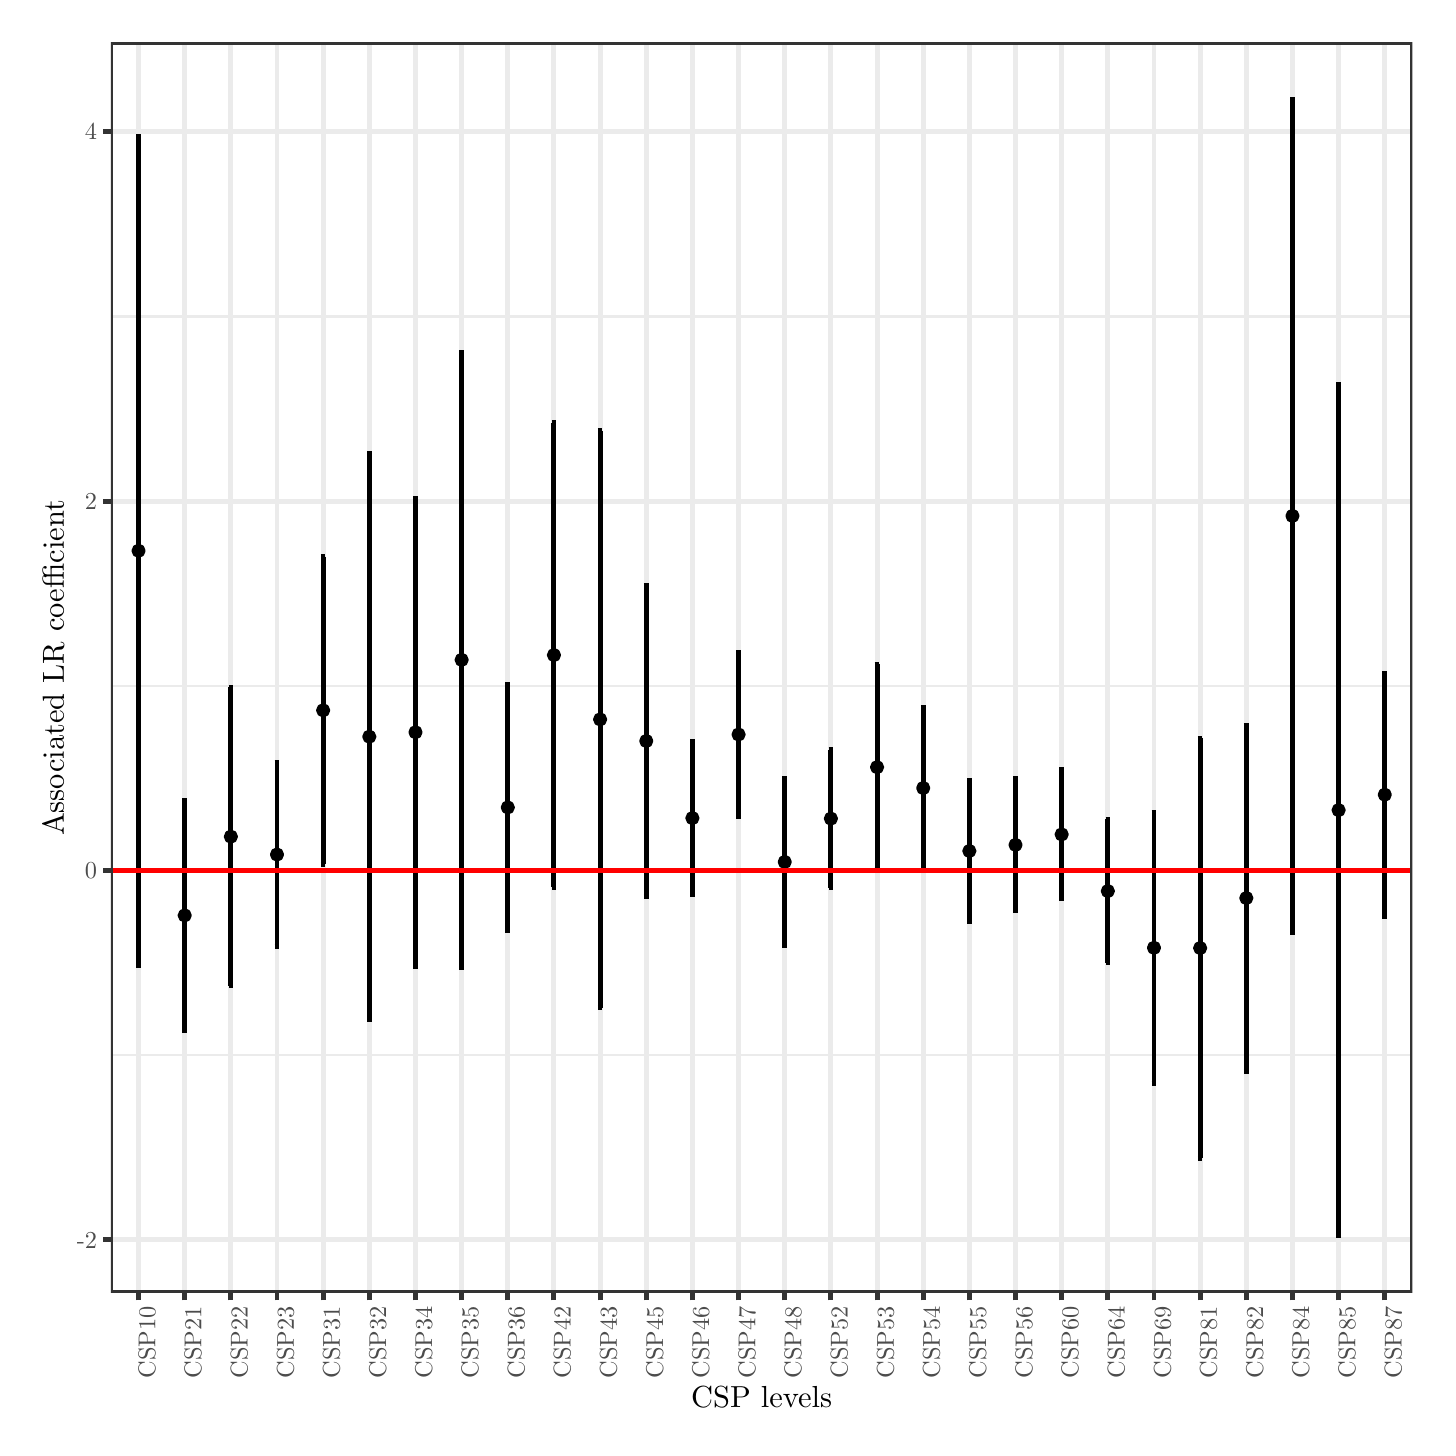
\begin{tikzpicture}[x=1pt,y=1pt]
\definecolor{fillColor}{RGB}{255,255,255}
\path[use as bounding box,fill=fillColor,fill opacity=0.00] (0,0) rectangle (505.89,505.89);
\begin{scope}
\path[clip] (  0.00,  0.00) rectangle (505.89,505.89);
\definecolor{drawColor}{RGB}{255,255,255}
\definecolor{fillColor}{RGB}{255,255,255}

\path[draw=drawColor,line width= 1.8pt,line join=round,line cap=round,fill=fillColor] (  0.00,  0.00) rectangle (505.89,505.89);
\end{scope}
\begin{scope}
\path[clip] ( 30.05, 48.75) rectangle (500.39,500.39);
\definecolor{fillColor}{RGB}{255,255,255}

\path[fill=fillColor] ( 30.05, 48.75) rectangle (500.39,500.39);
\definecolor{drawColor}{gray}{0.92}

\path[draw=drawColor,line width= 0.9pt,line join=round] ( 30.05,134.58) --
	(500.39,134.58);

\path[draw=drawColor,line width= 0.9pt,line join=round] ( 30.05,268.08) --
	(500.39,268.08);

\path[draw=drawColor,line width= 0.9pt,line join=round] ( 30.05,401.59) --
	(500.39,401.59);

\path[draw=drawColor,line width= 1.8pt,line join=round] ( 30.05, 67.82) --
	(500.39, 67.82);

\path[draw=drawColor,line width= 1.8pt,line join=round] ( 30.05,201.33) --
	(500.39,201.33);

\path[draw=drawColor,line width= 1.8pt,line join=round] ( 30.05,334.84) --
	(500.39,334.84);

\path[draw=drawColor,line width= 1.8pt,line join=round] ( 30.05,468.35) --
	(500.39,468.35);

\path[draw=drawColor,line width= 1.8pt,line join=round] ( 40.06, 48.75) --
	( 40.06,500.39);

\path[draw=drawColor,line width= 1.8pt,line join=round] ( 56.74, 48.75) --
	( 56.74,500.39);

\path[draw=drawColor,line width= 1.8pt,line join=round] ( 73.42, 48.75) --
	( 73.42,500.39);

\path[draw=drawColor,line width= 1.8pt,line join=round] ( 90.09, 48.75) --
	( 90.09,500.39);

\path[draw=drawColor,line width= 1.8pt,line join=round] (106.77, 48.75) --
	(106.77,500.39);

\path[draw=drawColor,line width= 1.8pt,line join=round] (123.45, 48.75) --
	(123.45,500.39);

\path[draw=drawColor,line width= 1.8pt,line join=round] (140.13, 48.75) --
	(140.13,500.39);

\path[draw=drawColor,line width= 1.8pt,line join=round] (156.81, 48.75) --
	(156.81,500.39);

\path[draw=drawColor,line width= 1.8pt,line join=round] (173.49, 48.75) --
	(173.49,500.39);

\path[draw=drawColor,line width= 1.8pt,line join=round] (190.17, 48.75) --
	(190.17,500.39);

\path[draw=drawColor,line width= 1.8pt,line join=round] (206.85, 48.75) --
	(206.85,500.39);

\path[draw=drawColor,line width= 1.8pt,line join=round] (223.52, 48.75) --
	(223.52,500.39);

\path[draw=drawColor,line width= 1.8pt,line join=round] (240.20, 48.75) --
	(240.20,500.39);

\path[draw=drawColor,line width= 1.8pt,line join=round] (256.88, 48.75) --
	(256.88,500.39);

\path[draw=drawColor,line width= 1.8pt,line join=round] (273.56, 48.75) --
	(273.56,500.39);

\path[draw=drawColor,line width= 1.8pt,line join=round] (290.24, 48.75) --
	(290.24,500.39);

\path[draw=drawColor,line width= 1.8pt,line join=round] (306.92, 48.75) --
	(306.92,500.39);

\path[draw=drawColor,line width= 1.8pt,line join=round] (323.60, 48.75) --
	(323.60,500.39);

\path[draw=drawColor,line width= 1.8pt,line join=round] (340.27, 48.75) --
	(340.27,500.39);

\path[draw=drawColor,line width= 1.8pt,line join=round] (356.95, 48.75) --
	(356.95,500.39);

\path[draw=drawColor,line width= 1.8pt,line join=round] (373.63, 48.75) --
	(373.63,500.39);

\path[draw=drawColor,line width= 1.8pt,line join=round] (390.31, 48.75) --
	(390.31,500.39);

\path[draw=drawColor,line width= 1.8pt,line join=round] (406.99, 48.75) --
	(406.99,500.39);

\path[draw=drawColor,line width= 1.8pt,line join=round] (423.67, 48.75) --
	(423.67,500.39);

\path[draw=drawColor,line width= 1.8pt,line join=round] (440.35, 48.75) --
	(440.35,500.39);

\path[draw=drawColor,line width= 1.8pt,line join=round] (457.03, 48.75) --
	(457.03,500.39);

\path[draw=drawColor,line width= 1.8pt,line join=round] (473.70, 48.75) --
	(473.70,500.39);

\path[draw=drawColor,line width= 1.8pt,line join=round] (490.38, 48.75) --
	(490.38,500.39);
\definecolor{drawColor}{RGB}{0,0,0}

\path[draw=drawColor,line width= 1.8pt,line join=round] (239.37,247.82) --
	(241.04,247.82);

\path[draw=drawColor,line width= 1.8pt,line join=round] (240.20,247.82) --
	(240.20,192.71);

\path[draw=drawColor,line width= 1.8pt,line join=round] (239.37,192.71) --
	(241.04,192.71);

\path[draw=drawColor,line width= 1.8pt,line join=round] (356.12,234.41) --
	(357.79,234.41);

\path[draw=drawColor,line width= 1.8pt,line join=round] (356.95,234.41) --
	(356.95,186.76);

\path[draw=drawColor,line width= 1.8pt,line join=round] (356.12,186.76) --
	(357.79,186.76);

\path[draw=drawColor,line width= 1.8pt,line join=round] (105.94,314.77) --
	(107.61,314.77);

\path[draw=drawColor,line width= 1.8pt,line join=round] (106.77,314.77) --
	(106.77,203.67);

\path[draw=drawColor,line width= 1.8pt,line join=round] (105.94,203.67) --
	(107.61,203.67);

\path[draw=drawColor,line width= 1.8pt,line join=round] (372.80,237.67) --
	(374.47,237.67);

\path[draw=drawColor,line width= 1.8pt,line join=round] (373.63,237.67) --
	(373.63,191.07);

\path[draw=drawColor,line width= 1.8pt,line join=round] (372.80,191.07) --
	(374.47,191.07);

\path[draw=drawColor,line width= 1.8pt,line join=round] (339.44,233.68) --
	(341.11,233.68);

\path[draw=drawColor,line width= 1.8pt,line join=round] (340.27,233.68) --
	(340.27,183.07);

\path[draw=drawColor,line width= 1.8pt,line join=round] (339.44,183.07) --
	(341.11,183.07);

\path[draw=drawColor,line width= 1.8pt,line join=round] (172.65,268.58) --
	(174.32,268.58);

\path[draw=drawColor,line width= 1.8pt,line join=round] (173.49,268.58) --
	(173.49,179.67);

\path[draw=drawColor,line width= 1.8pt,line join=round] (172.65,179.67) --
	(174.32,179.67);

\path[draw=drawColor,line width= 1.8pt,line join=round] (439.51,253.90) --
	(441.18,253.90);

\path[draw=drawColor,line width= 1.8pt,line join=round] (440.35,253.90) --
	(440.35,128.85);

\path[draw=drawColor,line width= 1.8pt,line join=round] (439.51,128.85) --
	(441.18,128.85);

\path[draw=drawColor,line width= 1.8pt,line join=round] (289.40,245.02) --
	(291.07,245.02);

\path[draw=drawColor,line width= 1.8pt,line join=round] (290.24,245.02) --
	(290.24,195.15);

\path[draw=drawColor,line width= 1.8pt,line join=round] (289.40,195.15) --
	(291.07,195.15);

\path[draw=drawColor,line width= 1.8pt,line join=round] (256.05,280.02) --
	(257.72,280.02);

\path[draw=drawColor,line width= 1.8pt,line join=round] (256.88,280.02) --
	(256.88,220.93);

\path[draw=drawColor,line width= 1.8pt,line join=round] (256.05,220.93) --
	(257.72,220.93);

\path[draw=drawColor,line width= 1.8pt,line join=round] ( 55.90,226.67) --
	( 57.57,226.67);

\path[draw=drawColor,line width= 1.8pt,line join=round] ( 56.74,226.67) --
	( 56.74,143.54);

\path[draw=drawColor,line width= 1.8pt,line join=round] ( 55.90,143.54) --
	( 57.57,143.54);

\path[draw=drawColor,line width= 1.8pt,line join=round] (306.08,275.80) --
	(307.75,275.80);

\path[draw=drawColor,line width= 1.8pt,line join=round] (306.92,275.80) --
	(306.92,201.53);

\path[draw=drawColor,line width= 1.8pt,line join=round] (306.08,201.53) --
	(307.75,201.53);

\path[draw=drawColor,line width= 1.8pt,line join=round] (322.76,260.22) --
	(324.43,260.22);

\path[draw=drawColor,line width= 1.8pt,line join=round] (323.60,260.22) --
	(323.60,202.05);

\path[draw=drawColor,line width= 1.8pt,line join=round] (322.76,202.05) --
	(324.43,202.05);

\path[draw=drawColor,line width= 1.8pt,line join=round] ( 89.26,240.48) --
	( 90.93,240.48);

\path[draw=drawColor,line width= 1.8pt,line join=round] ( 90.09,240.48) --
	( 90.09,173.73);

\path[draw=drawColor,line width= 1.8pt,line join=round] ( 89.26,173.73) --
	( 90.93,173.73);

\path[draw=drawColor,line width= 1.8pt,line join=round] (422.83,249.20) --
	(424.50,249.20);

\path[draw=drawColor,line width= 1.8pt,line join=round] (423.67,249.20) --
	(423.67, 97.43);

\path[draw=drawColor,line width= 1.8pt,line join=round] (422.83, 97.43) --
	(424.50, 97.43);

\path[draw=drawColor,line width= 1.8pt,line join=round] (272.73,234.60) --
	(274.39,234.60);

\path[draw=drawColor,line width= 1.8pt,line join=round] (273.56,234.60) --
	(273.56,174.25);

\path[draw=drawColor,line width= 1.8pt,line join=round] (272.73,174.25) --
	(274.39,174.25);

\path[draw=drawColor,line width= 1.8pt,line join=round] (139.30,335.85) --
	(140.96,335.85);

\path[draw=drawColor,line width= 1.8pt,line join=round] (140.13,335.85) --
	(140.13,166.73);

\path[draw=drawColor,line width= 1.8pt,line join=round] (139.30,166.73) --
	(140.96,166.73);

\path[draw=drawColor,line width= 1.8pt,line join=round] (389.48,219.90) --
	(391.14,219.90);

\path[draw=drawColor,line width= 1.8pt,line join=round] (390.31,219.90) --
	(390.31,167.91);

\path[draw=drawColor,line width= 1.8pt,line join=round] (389.48,167.91) --
	(391.14,167.91);

\path[draw=drawColor,line width= 1.8pt,line join=round] (189.33,363.13) --
	(191.00,363.13);

\path[draw=drawColor,line width= 1.8pt,line join=round] (190.17,363.13) --
	(190.17,195.23);

\path[draw=drawColor,line width= 1.8pt,line join=round] (189.33,195.23) --
	(191.00,195.23);

\path[draw=drawColor,line width= 1.8pt,line join=round] (122.62,352.06) --
	(124.29,352.06);

\path[draw=drawColor,line width= 1.8pt,line join=round] (123.45,352.06) --
	(123.45,147.31);

\path[draw=drawColor,line width= 1.8pt,line join=round] (122.62,147.31) --
	(124.29,147.31);

\path[draw=drawColor,line width= 1.8pt,line join=round] (206.01,360.21) --
	(207.68,360.21);

\path[draw=drawColor,line width= 1.8pt,line join=round] (206.85,360.21) --
	(206.85,151.65);

\path[draw=drawColor,line width= 1.8pt,line join=round] (206.01,151.65) --
	(207.68,151.65);

\path[draw=drawColor,line width= 1.8pt,line join=round] (222.69,304.30) --
	(224.36,304.30);

\path[draw=drawColor,line width= 1.8pt,line join=round] (223.52,304.30) --
	(223.52,191.96);

\path[draw=drawColor,line width= 1.8pt,line join=round] (222.69,191.96) --
	(224.36,191.96);

\path[draw=drawColor,line width= 1.8pt,line join=round] (406.16,222.39) --
	(407.82,222.39);

\path[draw=drawColor,line width= 1.8pt,line join=round] (406.99,222.39) --
	(406.99,124.41);

\path[draw=drawColor,line width= 1.8pt,line join=round] (406.16,124.41) --
	(407.82,124.41);

\path[draw=drawColor,line width= 1.8pt,line join=round] ( 72.58,267.52) --
	( 74.25,267.52);

\path[draw=drawColor,line width= 1.8pt,line join=round] ( 73.42,267.52) --
	( 73.42,159.62);

\path[draw=drawColor,line width= 1.8pt,line join=round] ( 72.58,159.62) --
	( 74.25,159.62);

\path[draw=drawColor,line width= 1.8pt,line join=round] (155.98,388.62) --
	(157.64,388.62);

\path[draw=drawColor,line width= 1.8pt,line join=round] (156.81,388.62) --
	(156.81,166.28);

\path[draw=drawColor,line width= 1.8pt,line join=round] (155.98,166.28) --
	(157.64,166.28);

\path[draw=drawColor,line width= 1.8pt,line join=round] (456.19,479.86) --
	(457.86,479.86);

\path[draw=drawColor,line width= 1.8pt,line join=round] (457.03,479.86) --
	(457.03,179.07);

\path[draw=drawColor,line width= 1.8pt,line join=round] (456.19,179.07) --
	(457.86,179.07);

\path[draw=drawColor,line width= 1.8pt,line join=round] ( 39.22,466.63) --
	( 40.89,466.63);

\path[draw=drawColor,line width= 1.8pt,line join=round] ( 40.06,466.63) --
	( 40.06,167.09);

\path[draw=drawColor,line width= 1.8pt,line join=round] ( 39.22,167.09) --
	( 40.89,167.09);

\path[draw=drawColor,line width= 1.8pt,line join=round] (489.55,272.67) --
	(491.22,272.67);

\path[draw=drawColor,line width= 1.8pt,line join=round] (490.38,272.67) --
	(490.38,184.79);

\path[draw=drawColor,line width= 1.8pt,line join=round] (489.55,184.79) --
	(491.22,184.79);

\path[draw=drawColor,line width= 1.8pt,line join=round] (472.87,377.02) --
	(474.54,377.02);

\path[draw=drawColor,line width= 1.8pt,line join=round] (473.70,377.02) --
	(473.70, 69.28);

\path[draw=drawColor,line width= 1.8pt,line join=round] (472.87, 69.28) --
	(474.54, 69.28);
\definecolor{fillColor}{RGB}{0,0,0}

\path[draw=drawColor,line width= 1.2pt,line join=round,line cap=round,fill=fillColor] (240.20,220.27) circle (  1.96);

\path[draw=drawColor,line width= 1.2pt,line join=round,line cap=round,fill=fillColor] (356.95,210.59) circle (  1.96);

\path[draw=drawColor,line width= 1.2pt,line join=round,line cap=round,fill=fillColor] (106.77,259.22) circle (  1.96);

\path[draw=drawColor,line width= 1.2pt,line join=round,line cap=round,fill=fillColor] (373.63,214.37) circle (  1.96);

\path[draw=drawColor,line width= 1.2pt,line join=round,line cap=round,fill=fillColor] (340.27,208.38) circle (  1.96);

\path[draw=drawColor,line width= 1.2pt,line join=round,line cap=round,fill=fillColor] (173.49,224.12) circle (  1.96);

\path[draw=drawColor,line width= 1.2pt,line join=round,line cap=round,fill=fillColor] (440.35,191.38) circle (  1.96);

\path[draw=drawColor,line width= 1.2pt,line join=round,line cap=round,fill=fillColor] (290.24,220.09) circle (  1.96);

\path[draw=drawColor,line width= 1.2pt,line join=round,line cap=round,fill=fillColor] (256.88,250.48) circle (  1.96);

\path[draw=drawColor,line width= 1.2pt,line join=round,line cap=round,fill=fillColor] ( 56.74,185.11) circle (  1.96);

\path[draw=drawColor,line width= 1.2pt,line join=round,line cap=round,fill=fillColor] (306.92,238.67) circle (  1.96);

\path[draw=drawColor,line width= 1.2pt,line join=round,line cap=round,fill=fillColor] (323.60,231.13) circle (  1.96);

\path[draw=drawColor,line width= 1.2pt,line join=round,line cap=round,fill=fillColor] ( 90.09,207.10) circle (  1.96);

\path[draw=drawColor,line width= 1.2pt,line join=round,line cap=round,fill=fillColor] (423.67,173.32) circle (  1.96);

\path[draw=drawColor,line width= 1.2pt,line join=round,line cap=round,fill=fillColor] (273.56,204.43) circle (  1.96);

\path[draw=drawColor,line width= 1.2pt,line join=round,line cap=round,fill=fillColor] (140.13,251.29) circle (  1.96);

\path[draw=drawColor,line width= 1.2pt,line join=round,line cap=round,fill=fillColor] (390.31,193.90) circle (  1.96);

\path[draw=drawColor,line width= 1.2pt,line join=round,line cap=round,fill=fillColor] (190.17,279.18) circle (  1.96);

\path[draw=drawColor,line width= 1.2pt,line join=round,line cap=round,fill=fillColor] (123.45,249.69) circle (  1.96);

\path[draw=drawColor,line width= 1.2pt,line join=round,line cap=round,fill=fillColor] (206.85,255.93) circle (  1.96);

\path[draw=drawColor,line width= 1.2pt,line join=round,line cap=round,fill=fillColor] (223.52,248.13) circle (  1.96);

\path[draw=drawColor,line width= 1.2pt,line join=round,line cap=round,fill=fillColor] (406.99,173.40) circle (  1.96);

\path[draw=drawColor,line width= 1.2pt,line join=round,line cap=round,fill=fillColor] ( 73.42,213.57) circle (  1.96);

\path[draw=drawColor,line width= 1.2pt,line join=round,line cap=round,fill=fillColor] (156.81,277.45) circle (  1.96);

\path[draw=drawColor,line width= 1.2pt,line join=round,line cap=round,fill=fillColor] (457.03,329.46) circle (  1.96);

\path[draw=drawColor,line width= 1.2pt,line join=round,line cap=round,fill=fillColor] ( 40.06,316.86) circle (  1.96);

\path[draw=drawColor,line width= 1.2pt,line join=round,line cap=round,fill=fillColor] (490.38,228.73) circle (  1.96);

\path[draw=drawColor,line width= 1.2pt,line join=round,line cap=round,fill=fillColor] (473.70,223.15) circle (  1.96);
\definecolor{drawColor}{RGB}{255,0,0}

\path[draw=drawColor,line width= 1.8pt,line join=round] ( 30.05,201.33) -- (500.39,201.33);
\definecolor{drawColor}{gray}{0.20}

\path[draw=drawColor,line width= 1.8pt,line join=round,line cap=round] ( 30.05, 48.75) rectangle (500.39,500.39);
\end{scope}
\begin{scope}
\path[clip] (  0.00,  0.00) rectangle (505.89,505.89);
\definecolor{drawColor}{gray}{0.30}

\node[text=drawColor,anchor=base east,inner sep=0pt, outer sep=0pt, scale=  0.88] at ( 25.10, 64.79) {-2};

\node[text=drawColor,anchor=base east,inner sep=0pt, outer sep=0pt, scale=  0.88] at ( 25.10,198.30) {0};

\node[text=drawColor,anchor=base east,inner sep=0pt, outer sep=0pt, scale=  0.88] at ( 25.10,331.81) {2};

\node[text=drawColor,anchor=base east,inner sep=0pt, outer sep=0pt, scale=  0.88] at ( 25.10,465.32) {4};
\end{scope}
\begin{scope}
\path[clip] (  0.00,  0.00) rectangle (505.89,505.89);
\definecolor{drawColor}{gray}{0.20}

\path[draw=drawColor,line width= 1.8pt,line join=round] ( 27.30, 67.82) --
	( 30.05, 67.82);

\path[draw=drawColor,line width= 1.8pt,line join=round] ( 27.30,201.33) --
	( 30.05,201.33);

\path[draw=drawColor,line width= 1.8pt,line join=round] ( 27.30,334.84) --
	( 30.05,334.84);

\path[draw=drawColor,line width= 1.8pt,line join=round] ( 27.30,468.35) --
	( 30.05,468.35);
\end{scope}
\begin{scope}
\path[clip] (  0.00,  0.00) rectangle (505.89,505.89);
\definecolor{drawColor}{gray}{0.20}

\path[draw=drawColor,line width= 1.8pt,line join=round] ( 40.06, 46.00) --
	( 40.06, 48.75);

\path[draw=drawColor,line width= 1.8pt,line join=round] ( 56.74, 46.00) --
	( 56.74, 48.75);

\path[draw=drawColor,line width= 1.8pt,line join=round] ( 73.42, 46.00) --
	( 73.42, 48.75);

\path[draw=drawColor,line width= 1.8pt,line join=round] ( 90.09, 46.00) --
	( 90.09, 48.75);

\path[draw=drawColor,line width= 1.8pt,line join=round] (106.77, 46.00) --
	(106.77, 48.75);

\path[draw=drawColor,line width= 1.8pt,line join=round] (123.45, 46.00) --
	(123.45, 48.75);

\path[draw=drawColor,line width= 1.8pt,line join=round] (140.13, 46.00) --
	(140.13, 48.75);

\path[draw=drawColor,line width= 1.8pt,line join=round] (156.81, 46.00) --
	(156.81, 48.75);

\path[draw=drawColor,line width= 1.8pt,line join=round] (173.49, 46.00) --
	(173.49, 48.75);

\path[draw=drawColor,line width= 1.8pt,line join=round] (190.17, 46.00) --
	(190.17, 48.75);

\path[draw=drawColor,line width= 1.8pt,line join=round] (206.85, 46.00) --
	(206.85, 48.75);

\path[draw=drawColor,line width= 1.8pt,line join=round] (223.52, 46.00) --
	(223.52, 48.75);

\path[draw=drawColor,line width= 1.8pt,line join=round] (240.20, 46.00) --
	(240.20, 48.75);

\path[draw=drawColor,line width= 1.8pt,line join=round] (256.88, 46.00) --
	(256.88, 48.75);

\path[draw=drawColor,line width= 1.8pt,line join=round] (273.56, 46.00) --
	(273.56, 48.75);

\path[draw=drawColor,line width= 1.8pt,line join=round] (290.24, 46.00) --
	(290.24, 48.75);

\path[draw=drawColor,line width= 1.8pt,line join=round] (306.92, 46.00) --
	(306.92, 48.75);

\path[draw=drawColor,line width= 1.8pt,line join=round] (323.60, 46.00) --
	(323.60, 48.75);

\path[draw=drawColor,line width= 1.8pt,line join=round] (340.27, 46.00) --
	(340.27, 48.75);

\path[draw=drawColor,line width= 1.8pt,line join=round] (356.95, 46.00) --
	(356.95, 48.75);

\path[draw=drawColor,line width= 1.8pt,line join=round] (373.63, 46.00) --
	(373.63, 48.75);

\path[draw=drawColor,line width= 1.8pt,line join=round] (390.31, 46.00) --
	(390.31, 48.75);

\path[draw=drawColor,line width= 1.8pt,line join=round] (406.99, 46.00) --
	(406.99, 48.75);

\path[draw=drawColor,line width= 1.8pt,line join=round] (423.67, 46.00) --
	(423.67, 48.75);

\path[draw=drawColor,line width= 1.8pt,line join=round] (440.35, 46.00) --
	(440.35, 48.75);

\path[draw=drawColor,line width= 1.8pt,line join=round] (457.03, 46.00) --
	(457.03, 48.75);

\path[draw=drawColor,line width= 1.8pt,line join=round] (473.70, 46.00) --
	(473.70, 48.75);

\path[draw=drawColor,line width= 1.8pt,line join=round] (490.38, 46.00) --
	(490.38, 48.75);
\end{scope}
\begin{scope}
\path[clip] (  0.00,  0.00) rectangle (505.89,505.89);
\definecolor{drawColor}{gray}{0.30}

\node[text=drawColor,rotate= 90.00,anchor=base east,inner sep=0pt, outer sep=0pt, scale=  0.88] at ( 46.12, 43.80) {CSP10};

\node[text=drawColor,rotate= 90.00,anchor=base east,inner sep=0pt, outer sep=0pt, scale=  0.88] at ( 62.80, 43.80) {CSP21};

\node[text=drawColor,rotate= 90.00,anchor=base east,inner sep=0pt, outer sep=0pt, scale=  0.88] at ( 79.48, 43.80) {CSP22};

\node[text=drawColor,rotate= 90.00,anchor=base east,inner sep=0pt, outer sep=0pt, scale=  0.88] at ( 96.16, 43.80) {CSP23};

\node[text=drawColor,rotate= 90.00,anchor=base east,inner sep=0pt, outer sep=0pt, scale=  0.88] at (112.83, 43.80) {CSP31};

\node[text=drawColor,rotate= 90.00,anchor=base east,inner sep=0pt, outer sep=0pt, scale=  0.88] at (129.51, 43.80) {CSP32};

\node[text=drawColor,rotate= 90.00,anchor=base east,inner sep=0pt, outer sep=0pt, scale=  0.88] at (146.19, 43.80) {CSP34};

\node[text=drawColor,rotate= 90.00,anchor=base east,inner sep=0pt, outer sep=0pt, scale=  0.88] at (162.87, 43.80) {CSP35};

\node[text=drawColor,rotate= 90.00,anchor=base east,inner sep=0pt, outer sep=0pt, scale=  0.88] at (179.55, 43.80) {CSP36};

\node[text=drawColor,rotate= 90.00,anchor=base east,inner sep=0pt, outer sep=0pt, scale=  0.88] at (196.23, 43.80) {CSP42};

\node[text=drawColor,rotate= 90.00,anchor=base east,inner sep=0pt, outer sep=0pt, scale=  0.88] at (212.91, 43.80) {CSP43};

\node[text=drawColor,rotate= 90.00,anchor=base east,inner sep=0pt, outer sep=0pt, scale=  0.88] at (229.58, 43.80) {CSP45};

\node[text=drawColor,rotate= 90.00,anchor=base east,inner sep=0pt, outer sep=0pt, scale=  0.88] at (246.26, 43.80) {CSP46};

\node[text=drawColor,rotate= 90.00,anchor=base east,inner sep=0pt, outer sep=0pt, scale=  0.88] at (262.94, 43.80) {CSP47};

\node[text=drawColor,rotate= 90.00,anchor=base east,inner sep=0pt, outer sep=0pt, scale=  0.88] at (279.62, 43.80) {CSP48};

\node[text=drawColor,rotate= 90.00,anchor=base east,inner sep=0pt, outer sep=0pt, scale=  0.88] at (296.30, 43.80) {CSP52};

\node[text=drawColor,rotate= 90.00,anchor=base east,inner sep=0pt, outer sep=0pt, scale=  0.88] at (312.98, 43.80) {CSP53};

\node[text=drawColor,rotate= 90.00,anchor=base east,inner sep=0pt, outer sep=0pt, scale=  0.88] at (329.66, 43.80) {CSP54};

\node[text=drawColor,rotate= 90.00,anchor=base east,inner sep=0pt, outer sep=0pt, scale=  0.88] at (346.34, 43.80) {CSP55};

\node[text=drawColor,rotate= 90.00,anchor=base east,inner sep=0pt, outer sep=0pt, scale=  0.88] at (363.01, 43.80) {CSP56};

\node[text=drawColor,rotate= 90.00,anchor=base east,inner sep=0pt, outer sep=0pt, scale=  0.88] at (379.69, 43.80) {CSP60};

\node[text=drawColor,rotate= 90.00,anchor=base east,inner sep=0pt, outer sep=0pt, scale=  0.88] at (396.37, 43.80) {CSP64};

\node[text=drawColor,rotate= 90.00,anchor=base east,inner sep=0pt, outer sep=0pt, scale=  0.88] at (413.05, 43.80) {CSP69};

\node[text=drawColor,rotate= 90.00,anchor=base east,inner sep=0pt, outer sep=0pt, scale=  0.88] at (429.73, 43.80) {CSP81};

\node[text=drawColor,rotate= 90.00,anchor=base east,inner sep=0pt, outer sep=0pt, scale=  0.88] at (446.41, 43.80) {CSP82};

\node[text=drawColor,rotate= 90.00,anchor=base east,inner sep=0pt, outer sep=0pt, scale=  0.88] at (463.09, 43.80) {CSP84};

\node[text=drawColor,rotate= 90.00,anchor=base east,inner sep=0pt, outer sep=0pt, scale=  0.88] at (479.76, 43.80) {CSP85};

\node[text=drawColor,rotate= 90.00,anchor=base east,inner sep=0pt, outer sep=0pt, scale=  0.88] at (496.44, 43.80) {CSP87};
\end{scope}
\begin{scope}
\path[clip] (  0.00,  0.00) rectangle (505.89,505.89);
\definecolor{drawColor}{RGB}{0,0,0}

\node[text=drawColor,anchor=base,inner sep=0pt, outer sep=0pt, scale=  1.10] at (265.22,  7.44) {CSP levels};
\end{scope}
\begin{scope}
\path[clip] (  0.00,  0.00) rectangle (505.89,505.89);
\definecolor{drawColor}{RGB}{0,0,0}

\node[text=drawColor,rotate= 90.00,anchor=base,inner sep=0pt, outer sep=0pt, scale=  1.10] at ( 13.08,274.57) {Associated LR coefficient};
\end{scope}
\end{tikzpicture}
}
\caption{Having a lot of levels means having lots of coefficients, few of which are significant.}
\label{fig:csp_estim}
\end{subfigure}
\begin{subfigure}[t]{0.5\textwidth}
\centering \resizebox{\textwidth}{!}{% Created by tikzDevice version 0.12 on 2019-03-11 09:44:28
% !TEX encoding = UTF-8 Unicode
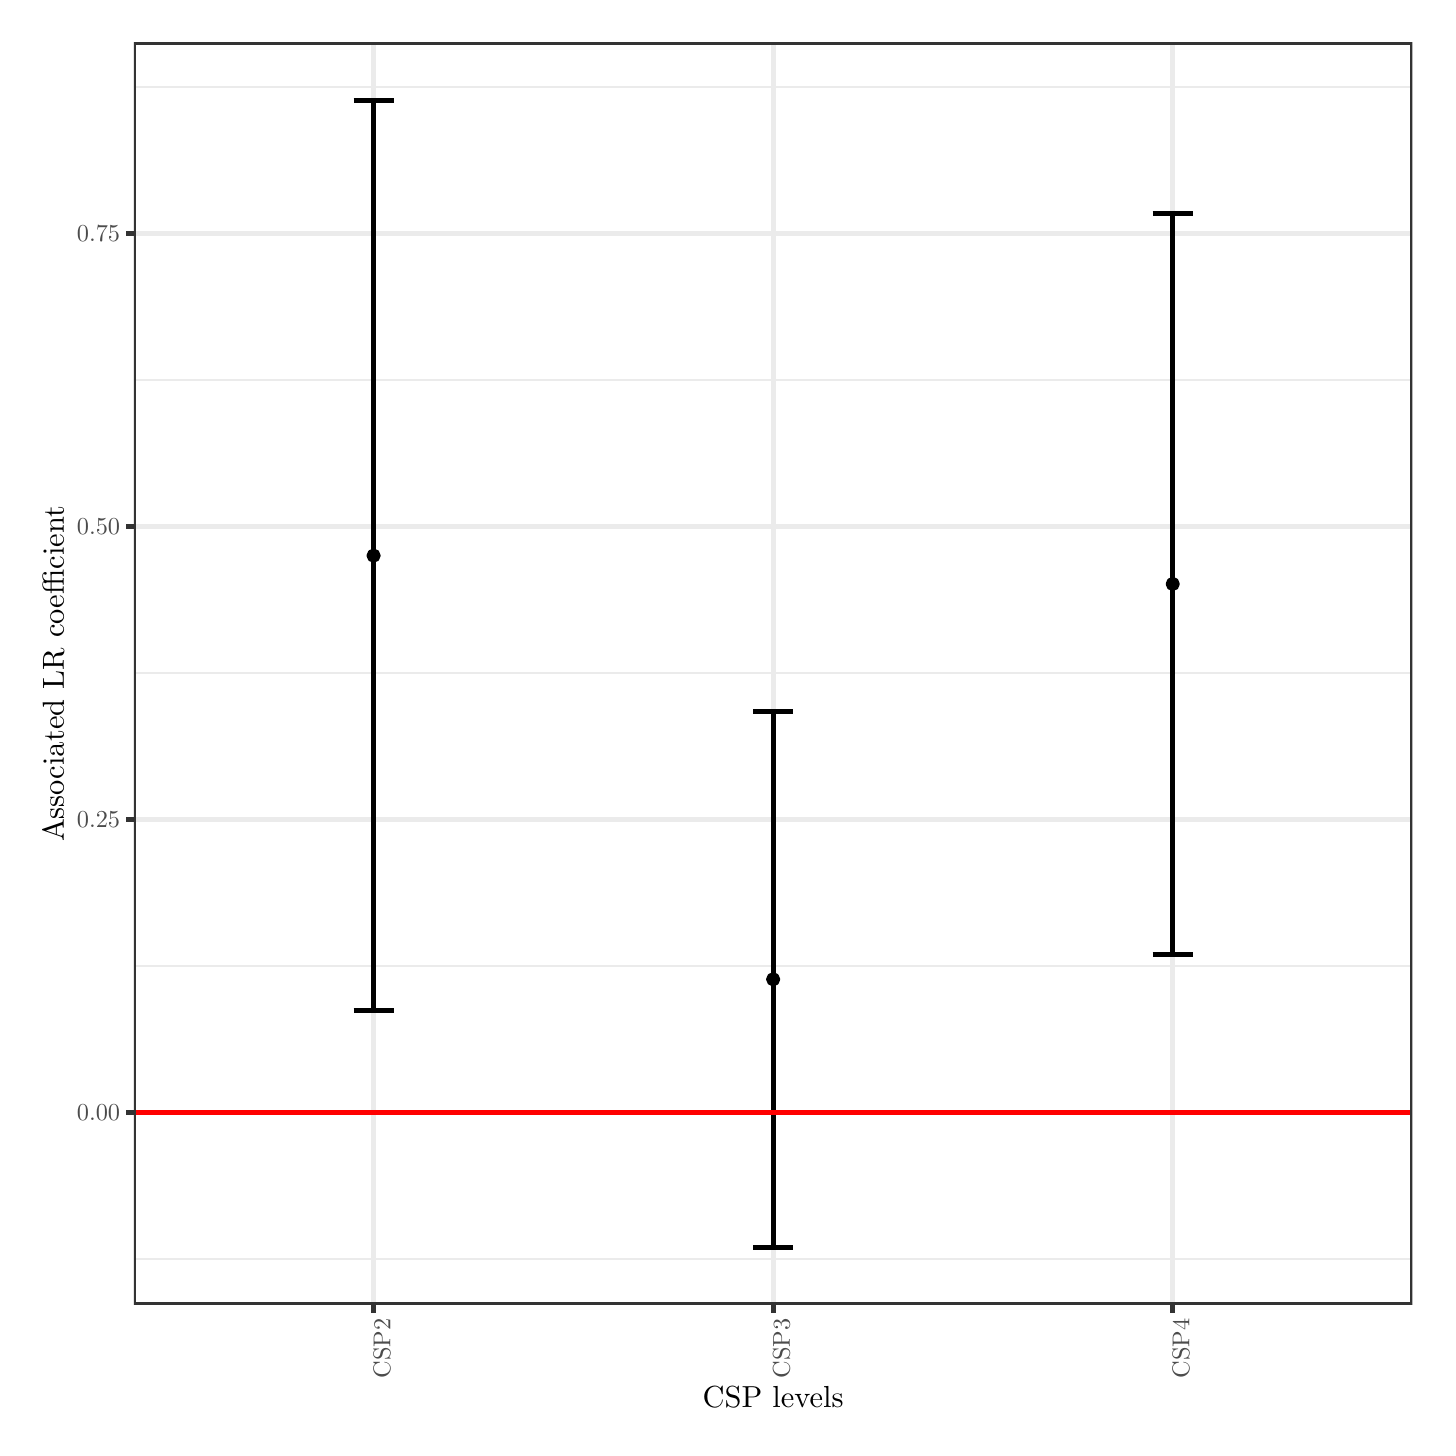
\begin{tikzpicture}[x=1pt,y=1pt]
\definecolor{fillColor}{RGB}{255,255,255}
\path[use as bounding box,fill=fillColor,fill opacity=0.00] (0,0) rectangle (505.89,505.89);
\begin{scope}
\path[clip] (  0.00,  0.00) rectangle (505.89,505.89);
\definecolor{drawColor}{RGB}{255,255,255}
\definecolor{fillColor}{RGB}{255,255,255}

\path[draw=drawColor,line width= 1.8pt,line join=round,line cap=round,fill=fillColor] (  0.00,  0.00) rectangle (505.89,505.89);
\end{scope}
\begin{scope}
\path[clip] ( 38.36, 44.35) rectangle (500.39,500.39);
\definecolor{fillColor}{RGB}{255,255,255}

\path[fill=fillColor] ( 38.36, 44.35) rectangle (500.39,500.39);
\definecolor{drawColor}{gray}{0.92}

\path[draw=drawColor,line width= 0.9pt,line join=round] ( 38.36, 60.90) --
	(500.39, 60.90);

\path[draw=drawColor,line width= 0.9pt,line join=round] ( 38.36,166.79) --
	(500.39,166.79);

\path[draw=drawColor,line width= 0.9pt,line join=round] ( 38.36,272.69) --
	(500.39,272.69);

\path[draw=drawColor,line width= 0.9pt,line join=round] ( 38.36,378.58) --
	(500.39,378.58);

\path[draw=drawColor,line width= 0.9pt,line join=round] ( 38.36,484.48) --
	(500.39,484.48);

\path[draw=drawColor,line width= 1.8pt,line join=round] ( 38.36,113.85) --
	(500.39,113.85);

\path[draw=drawColor,line width= 1.8pt,line join=round] ( 38.36,219.74) --
	(500.39,219.74);

\path[draw=drawColor,line width= 1.8pt,line join=round] ( 38.36,325.64) --
	(500.39,325.64);

\path[draw=drawColor,line width= 1.8pt,line join=round] ( 38.36,431.53) --
	(500.39,431.53);

\path[draw=drawColor,line width= 1.8pt,line join=round] (124.99, 44.35) --
	(124.99,500.39);

\path[draw=drawColor,line width= 1.8pt,line join=round] (269.38, 44.35) --
	(269.38,500.39);

\path[draw=drawColor,line width= 1.8pt,line join=round] (413.76, 44.35) --
	(413.76,500.39);
\definecolor{drawColor}{RGB}{0,0,0}

\path[draw=drawColor,line width= 1.8pt,line join=round] (117.77,479.66) --
	(132.21,479.66);

\path[draw=drawColor,line width= 1.8pt,line join=round] (124.99,479.66) --
	(124.99,150.57);

\path[draw=drawColor,line width= 1.8pt,line join=round] (117.77,150.57) --
	(132.21,150.57);

\path[draw=drawColor,line width= 1.8pt,line join=round] (262.16,258.96) --
	(276.59,258.96);

\path[draw=drawColor,line width= 1.8pt,line join=round] (269.38,258.96) --
	(269.38, 65.08);

\path[draw=drawColor,line width= 1.8pt,line join=round] (262.16, 65.08) --
	(276.59, 65.08);

\path[draw=drawColor,line width= 1.8pt,line join=round] (406.54,438.77) --
	(420.98,438.77);

\path[draw=drawColor,line width= 1.8pt,line join=round] (413.76,438.77) --
	(413.76,170.98);

\path[draw=drawColor,line width= 1.8pt,line join=round] (406.54,170.98) --
	(420.98,170.98);
\definecolor{fillColor}{RGB}{0,0,0}

\path[draw=drawColor,line width= 1.2pt,line join=round,line cap=round,fill=fillColor] (124.99,315.11) circle (  1.96);

\path[draw=drawColor,line width= 1.2pt,line join=round,line cap=round,fill=fillColor] (269.38,162.02) circle (  1.96);

\path[draw=drawColor,line width= 1.2pt,line join=round,line cap=round,fill=fillColor] (413.76,304.87) circle (  1.96);
\definecolor{drawColor}{RGB}{255,0,0}

\path[draw=drawColor,line width= 1.8pt,line join=round] ( 38.36,113.85) -- (500.39,113.85);
\definecolor{drawColor}{gray}{0.20}

\path[draw=drawColor,line width= 1.8pt,line join=round,line cap=round] ( 38.36, 44.35) rectangle (500.39,500.39);
\end{scope}
\begin{scope}
\path[clip] (  0.00,  0.00) rectangle (505.89,505.89);
\definecolor{drawColor}{gray}{0.30}

\node[text=drawColor,anchor=base east,inner sep=0pt, outer sep=0pt, scale=  0.88] at ( 33.41,110.82) {0.00};

\node[text=drawColor,anchor=base east,inner sep=0pt, outer sep=0pt, scale=  0.88] at ( 33.41,216.71) {0.25};

\node[text=drawColor,anchor=base east,inner sep=0pt, outer sep=0pt, scale=  0.88] at ( 33.41,322.61) {0.50};

\node[text=drawColor,anchor=base east,inner sep=0pt, outer sep=0pt, scale=  0.88] at ( 33.41,428.50) {0.75};
\end{scope}
\begin{scope}
\path[clip] (  0.00,  0.00) rectangle (505.89,505.89);
\definecolor{drawColor}{gray}{0.20}

\path[draw=drawColor,line width= 1.8pt,line join=round] ( 35.61,113.85) --
	( 38.36,113.85);

\path[draw=drawColor,line width= 1.8pt,line join=round] ( 35.61,219.74) --
	( 38.36,219.74);

\path[draw=drawColor,line width= 1.8pt,line join=round] ( 35.61,325.64) --
	( 38.36,325.64);

\path[draw=drawColor,line width= 1.8pt,line join=round] ( 35.61,431.53) --
	( 38.36,431.53);
\end{scope}
\begin{scope}
\path[clip] (  0.00,  0.00) rectangle (505.89,505.89);
\definecolor{drawColor}{gray}{0.20}

\path[draw=drawColor,line width= 1.8pt,line join=round] (124.99, 41.60) --
	(124.99, 44.35);

\path[draw=drawColor,line width= 1.8pt,line join=round] (269.38, 41.60) --
	(269.38, 44.35);

\path[draw=drawColor,line width= 1.8pt,line join=round] (413.76, 41.60) --
	(413.76, 44.35);
\end{scope}
\begin{scope}
\path[clip] (  0.00,  0.00) rectangle (505.89,505.89);
\definecolor{drawColor}{gray}{0.30}

\node[text=drawColor,rotate= 90.00,anchor=base east,inner sep=0pt, outer sep=0pt, scale=  0.88] at (131.05, 39.40) {CSP2};

\node[text=drawColor,rotate= 90.00,anchor=base east,inner sep=0pt, outer sep=0pt, scale=  0.88] at (275.44, 39.40) {CSP3};

\node[text=drawColor,rotate= 90.00,anchor=base east,inner sep=0pt, outer sep=0pt, scale=  0.88] at (419.82, 39.40) {CSP4};
\end{scope}
\begin{scope}
\path[clip] (  0.00,  0.00) rectangle (505.89,505.89);
\definecolor{drawColor}{RGB}{0,0,0}

\node[text=drawColor,anchor=base,inner sep=0pt, outer sep=0pt, scale=  1.10] at (269.38,  7.44) {CSP levels};
\end{scope}
\begin{scope}
\path[clip] (  0.00,  0.00) rectangle (505.89,505.89);
\definecolor{drawColor}{RGB}{0,0,0}

\node[text=drawColor,rotate= 90.00,anchor=base,inner sep=0pt, outer sep=0pt, scale=  1.10] at ( 13.08,272.37) {Associated LR coefficient};
\end{scope}
\end{tikzpicture}
}
\caption{By grouping levels, fewer coefficients are obtained, which variance is significantly smaller and are thus significant.}
\label{fig:csp_estim_disc}
\end{subfigure}
\end{figure}

\section{Illustration of the bias-variance quantization tradeoff} \label{sec:bias_variance_quant}
 

The previous section motivated the use of quantization on a practical level. On a theoretical level, at least in terms of probability theory, quantization is equivalent to throwing away information: for continuous features, it is only known that they belong to a certain interval and for categorical features, their granularity among the original levels is lost.

However, two things must appear clearly: first, we are in a ``statistical'' setting, \textit{i.e.}\ finite-dimensional setting, where variance of estimation can play a big role, as was developed in Section~\ref{subsec:gradient}, which partly justifies the need to regroup categorical levels. Second, we are in a predictive setting, with an imposed classification model $p_{\glssymbol{bth}}$. I focus on logistic regression, for which continuous features get a single coefficient: their relationship with the logit transform of the probability of an event (bad borrower) is assumed to be linear which can yield model bias. Thus, having several coefficients per feature, which can be achieved with a  variety of techniques (\textit{e.g.}\ splines), can yield a lower model bias (when the true model is not linear, which is generally the case for \textit{Credit Scoring} data) at the cost of increased variance of estimation.

This phenomenon can be very simply captured by a small simulation: in the misspecified model setting, where the logit transform is assumed to stem from a sinusoidal transformation of $x$ on $[0;1]$, it can clearly be seen from Figure~\ref{fig:sinus_lin} that a standard linear logistic regression does poorly. Discretizing the feature $x$ results, using a very simple unsupervised heuristic named \textit{equal-length} (described in-depth in Appendix~\ref{app1:equal_length}), in good results (\textit{i.e.}\ visually mild bias / low variance) so long as the number of intervals, and subsequently of logistic regression coefficients, is low (see Animation on Figure~\ref{fig:anim_sinus} or still on Figure~\ref{fig:sinus_deb}). When the number of intervals gets large, the bias gets low (the sinus is well approximated by the little step functions), but the variance gets bigger (see Animation on Figure~\ref{fig:anim_sinus} or still on Figure~\ref{fig:sinus_fin}).


\textcolor{red}{décommenter animation}

%\begin{figure}[!ht]
%\begin{animateinline}[poster=first, controls=all, palindrome, autopause, autoresume, width=\textwidth, height=7cm]{3}
%\multiframe{99}{i=2+1}{\input{R_CODE_FIGURES/chapitre4/disc_plot\i.tex}}%
%\end{animateinline}
%\caption{\label{fig:anim_sinus} Animation of logistic regression fits on data generated by a sinus with a number of discretization steps in the \textit{equal-length} algorithm ranging from 2 to 100.}
%\end{figure}

\begin{figure}[!ht]
\vspace*{-1cm}
\begin{subfigure}[t]{\textwidth}
\resizebox{\textwidth}{7cm}{\input{R_CODE_FIGURES/chapitre4/linear_plot.tex}}
\vspace*{-1cm}
\caption{\label{fig:sinus_lin} Linear logistic regression (in \textcolor{red}{red}) fit on data generated by a sinus (in \textcolor{green}{green}).}
\end{subfigure}
\vspace*{-1cm}
\begin{subfigure}[t]{\textwidth}
\resizebox{\textwidth}{7cm}{% Created by tikzDevice version 0.11 on 2019-01-04 16:37:42
% !TEX encoding = UTF-8 Unicode
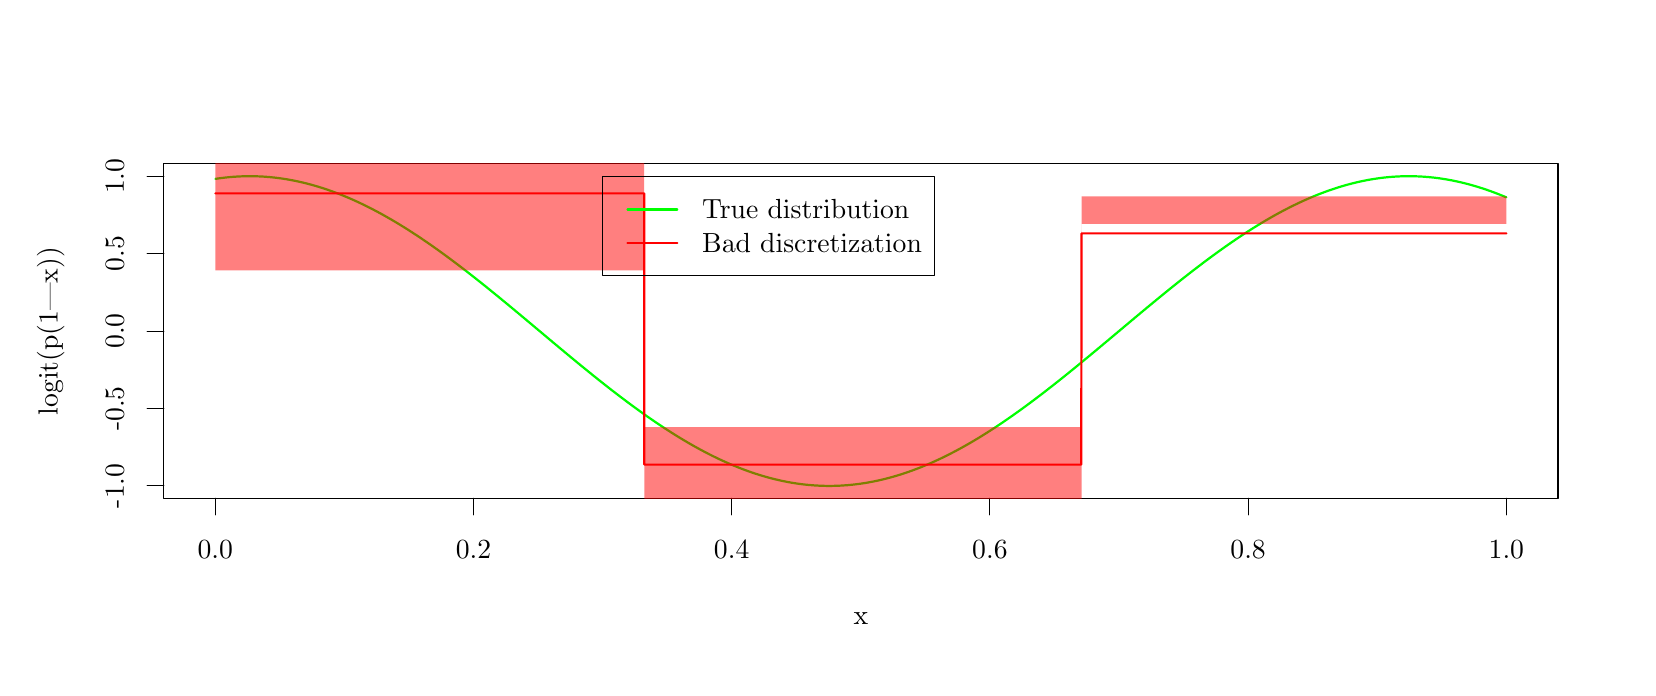
\begin{tikzpicture}[x=1pt,y=1pt]
\definecolor{fillColor}{RGB}{255,255,255}
\path[use as bounding box,fill=fillColor,fill opacity=0.00] (0,0) rectangle (578.16,231.26);
\begin{scope}
\path[clip] ( 49.20, 61.20) rectangle (552.96,182.06);
\definecolor{drawColor}{RGB}{0,255,0}

\path[draw=drawColor,line width= 0.8pt,line join=round,line cap=round] ( 67.86,176.62) --
	( 68.03,176.65) --
	( 68.05,176.65) --
	( 68.07,176.65) --
	( 68.24,176.68) --
	( 68.31,176.69) --
	( 68.32,176.69) --
	( 68.35,176.70) --
	( 68.38,176.70) --
	( 68.40,176.70) --
	( 68.40,176.70) --
	( 68.45,176.71) --
	( 68.53,176.72) --
	( 68.62,176.74) --
	( 68.67,176.74) --
	( 68.71,176.75) --
	( 68.75,176.75) --
	( 68.97,176.79) --
	( 69.08,176.80) --
	( 69.31,176.83) --
	( 69.37,176.84) --
	( 69.43,176.85) --
	( 69.49,176.86) --
	( 69.51,176.86) --
	( 69.55,176.87) --
	( 69.76,176.89) --
	( 69.78,176.90) --
	( 69.96,176.92) --
	( 69.99,176.92) --
	( 70.15,176.94) --
	( 70.28,176.96) --
	( 70.35,176.97) --
	( 70.44,176.98) --
	( 70.55,176.99) --
	( 70.57,177.00) --
	( 70.78,177.02) --
	( 70.90,177.04) --
	( 71.15,177.06) --
	( 71.16,177.07) --
	( 71.17,177.07) --
	( 71.26,177.08) --
	( 71.34,177.09) --
	( 71.46,177.10) --
	( 71.56,177.11) --
	( 71.57,177.11) --
	( 71.57,177.11) --
	( 71.90,177.15) --
	( 71.91,177.15) --
	( 72.17,177.17) --
	( 72.23,177.18) --
	( 72.35,177.19) --
	( 72.36,177.19) --
	( 72.43,177.20) --
	( 72.49,177.21) --
	( 72.51,177.21) --
	( 72.69,177.23) --
	( 72.73,177.23) --
	( 72.89,177.25) --
	( 72.91,177.25) --
	( 72.93,177.25) --
	( 72.94,177.25) --
	( 72.97,177.25) --
	( 73.06,177.26) --
	( 73.25,177.28) --
	( 73.44,177.29) --
	( 73.50,177.30) --
	( 73.54,177.30) --
	( 73.62,177.31) --
	( 73.75,177.32) --
	( 73.85,177.33) --
	( 73.87,177.33) --
	( 73.88,177.33) --
	( 73.93,177.33) --
	( 73.96,177.34) --
	( 74.01,177.34) --
	( 74.07,177.35) --
	( 74.22,177.36) --
	( 74.41,177.37) --
	( 74.42,177.37) --
	( 74.54,177.38) --
	( 74.73,177.39) --
	( 74.81,177.40) --
	( 74.96,177.41) --
	( 75.07,177.42) --
	( 75.15,177.42) --
	( 75.34,177.43) --
	( 75.52,177.45) --
	( 75.56,177.45) --
	( 75.64,177.45) --
	( 75.71,177.46) --
	( 75.81,177.46) --
	( 75.82,177.46) --
	( 75.83,177.46) --
	( 75.92,177.47) --
	( 75.97,177.47) --
	( 76.14,177.48) --
	( 76.21,177.48) --
	( 76.25,177.49) --
	( 76.25,177.49) --
	( 76.29,177.49) --
	( 76.34,177.49) --
	( 76.40,177.49) --
	( 76.42,177.49) --
	( 76.46,177.50) --
	( 76.56,177.50) --
	( 76.58,177.50) --
	( 76.72,177.51) --
	( 76.72,177.51) --
	( 77.03,177.52) --
	( 77.27,177.53) --
	( 77.37,177.53) --
	( 77.46,177.54) --
	( 77.50,177.54) --
	( 77.52,177.54) --
	( 77.53,177.54) --
	( 77.54,177.54) --
	( 77.57,177.54) --
	( 77.73,177.55) --
	( 77.79,177.55) --
	( 77.88,177.55) --
	( 77.93,177.55) --
	( 78.35,177.56) --
	( 78.37,177.56) --
	( 78.56,177.57) --
	( 78.56,177.57) --
	( 78.65,177.57) --
	( 78.79,177.57) --
	( 79.00,177.58) --
	( 79.01,177.58) --
	( 79.08,177.58) --
	( 79.12,177.58) --
	( 79.14,177.58) --
	( 79.23,177.58) --
	( 79.36,177.58) --
	( 79.50,177.58) --
	( 79.53,177.58) --
	( 79.60,177.58) --
	( 79.65,177.59) --
	( 79.70,177.59) --
	( 79.84,177.59) --
	( 79.84,177.59) --
	( 79.87,177.59) --
	( 80.00,177.59) --
	( 80.45,177.59) --
	( 80.50,177.59) --
	( 80.58,177.59) --
	( 80.59,177.59) --
	( 80.59,177.59) --
	( 80.70,177.59) --
	( 80.72,177.59) --
	( 80.73,177.59) --
	( 80.79,177.59) --
	( 80.90,177.59) --
	( 80.94,177.58) --
	( 80.95,177.58) --
	( 80.95,177.58) --
	( 81.00,177.58) --
	( 81.01,177.58) --
	( 81.04,177.58) --
	( 81.11,177.58) --
	( 81.47,177.58) --
	( 81.53,177.58) --
	( 81.77,177.57) --
	( 81.81,177.57) --
	( 81.82,177.57) --
	( 81.88,177.57) --
	( 81.97,177.57) --
	( 82.02,177.57) --
	( 82.07,177.57) --
	( 82.11,177.57) --
	( 82.13,177.57) --
	( 82.14,177.57) --
	( 82.18,177.56) --
	( 82.18,177.56) --
	( 82.54,177.56) --
	( 82.56,177.55) --
	( 82.56,177.55) --
	( 82.62,177.55) --
	( 82.75,177.55) --
	( 82.92,177.54) --
	( 83.12,177.54) --
	( 83.15,177.54) --
	( 83.17,177.53) --
	( 83.30,177.53) --
	( 83.32,177.53) --
	( 83.53,177.52) --
	( 83.59,177.52) --
	( 83.71,177.51) --
	( 83.83,177.51) --
	( 83.89,177.51) --
	( 83.90,177.50) --
	( 83.94,177.50) --
	( 84.02,177.50) --
	( 84.15,177.49) --
	( 84.22,177.49) --
	( 84.35,177.48) --
	( 84.35,177.48) --
	( 84.50,177.47) --
	( 84.54,177.47) --
	( 84.54,177.47) --
	( 84.65,177.47) --
	( 84.72,177.46) --
	( 84.72,177.46) --
	( 84.78,177.46) --
	( 84.81,177.46) --
	( 84.83,177.46) --
	( 84.85,177.46) --
	( 84.87,177.45) --
	( 84.90,177.45) --
	( 84.94,177.45) --
	( 84.98,177.45) --
	( 85.02,177.45) --
	( 85.17,177.44) --
	( 85.41,177.42) --
	( 85.45,177.42) --
	( 85.46,177.42) --
	( 85.59,177.41) --
	( 85.60,177.41) --
	( 85.72,177.40) --
	( 85.74,177.40) --
	( 85.90,177.39) --
	( 85.93,177.39) --
	( 86.01,177.38) --
	( 86.05,177.38) --
	( 86.08,177.38) --
	( 86.29,177.36) --
	( 86.41,177.35) --
	( 86.64,177.33) --
	( 86.87,177.31) --
	( 86.95,177.31) --
	( 86.97,177.31) --
	( 87.08,177.30) --
	( 87.14,177.29) --
	( 87.16,177.29) --
	( 87.28,177.28) --
	( 87.41,177.27) --
	( 87.67,177.24) --
	( 87.71,177.24) --
	( 87.77,177.23) --
	( 87.91,177.22) --
	( 87.93,177.22) --
	( 87.95,177.22) --
	( 88.15,177.20) --
	( 88.20,177.19) --
	( 88.41,177.17) --
	( 88.42,177.17) --
	( 88.61,177.15) --
	( 88.61,177.15) --
	( 88.67,177.14) --
	( 88.93,177.12) --
	( 89.06,177.10) --
	( 89.10,177.10) --
	( 89.17,177.09) --
	( 89.25,177.08) --
	( 89.36,177.07) --
	( 89.36,177.07) --
	( 89.39,177.06) --
	( 89.44,177.06) --
	( 89.47,177.05) --
	( 89.48,177.05) --
	( 89.93,177.00) --
	( 89.94,177.00) --
	( 90.14,176.98) --
	( 90.15,176.97) --
	( 90.20,176.97) --
	( 90.22,176.97) --
	( 90.25,176.96) --
	( 90.29,176.96) --
	( 90.47,176.93) --
	( 90.75,176.90) --
	( 90.75,176.90) --
	( 90.93,176.87) --
	( 90.95,176.87) --
	( 91.19,176.84) --
	( 91.24,176.83) --
	( 91.25,176.83) --
	( 91.30,176.82) --
	( 91.37,176.81) --
	( 91.38,176.81) --
	( 91.42,176.81) --
	( 91.45,176.80) --
	( 91.46,176.80) --
	( 91.48,176.80) --
	( 91.79,176.75) --
	( 91.84,176.75) --
	( 91.85,176.75) --
	( 92.06,176.71) --
	( 92.07,176.71) --
	( 92.10,176.71) --
	( 92.15,176.70) --
	( 92.22,176.69) --
	( 92.24,176.69) --
	( 92.30,176.68) --
	( 92.33,176.67) --
	( 92.37,176.67) --
	( 92.93,176.58) --
	( 93.05,176.56) --
	( 93.11,176.55) --
	( 93.11,176.55) --
	( 93.19,176.54) --
	( 93.21,176.54) --
	( 93.45,176.50) --
	( 93.49,176.49) --
	( 93.50,176.49) --
	( 93.68,176.46) --
	( 93.82,176.44) --
	( 93.82,176.43) --
	( 93.82,176.43) --
	( 93.85,176.43) --
	( 93.88,176.42) --
	( 94.00,176.40) --
	( 94.01,176.40) --
	( 94.09,176.39) --
	( 94.12,176.38) --
	( 94.14,176.38) --
	( 94.32,176.35) --
	( 94.53,176.31) --
	( 94.59,176.30) --
	( 94.70,176.28) --
	( 94.76,176.27) --
	( 94.77,176.27) --
	( 94.78,176.27) --
	( 94.79,176.26) --
	( 94.97,176.23) --
	( 95.02,176.22) --
	( 95.12,176.21) --
	( 95.19,176.19) --
	( 95.26,176.18) --
	( 95.26,176.18) --
	( 95.34,176.16) --
	( 95.63,176.11) --
	( 95.68,176.10) --
	( 95.71,176.09) --
	( 96.28,175.98) --
	( 96.28,175.98) --
	( 96.51,175.93) --
	( 96.59,175.92) --
	( 96.68,175.90) --
	( 96.68,175.90) --
	( 96.79,175.88) --
	( 96.87,175.86) --
	( 96.89,175.86) --
	( 96.92,175.85) --
	( 97.06,175.82) --
	( 97.13,175.81) --
	( 97.53,175.72) --
	( 97.53,175.72) --
	( 97.54,175.72) --
	( 97.56,175.72) --
	( 97.56,175.71) --
	( 97.82,175.66) --
	( 97.83,175.66) --
	( 97.84,175.65) --
	( 98.04,175.61) --
	( 98.07,175.60) --
	( 98.27,175.56) --
	( 98.30,175.55) --
	( 98.36,175.54) --
	( 98.47,175.52) --
	( 98.54,175.50) --
	( 98.61,175.48) --
	( 98.79,175.44) --
	( 98.83,175.43) --
	( 99.14,175.36) --
	( 99.16,175.35) --
	( 99.21,175.34) --
	( 99.33,175.31) --
	( 99.39,175.30) --
	( 99.50,175.28) --
	( 99.62,175.25) --
	( 99.63,175.24) --
	( 99.63,175.24) --
	( 99.70,175.23) --
	( 99.82,175.20) --
	( 99.84,175.19) --
	( 99.92,175.17) --
	( 99.99,175.16) --
	(100.30,175.08) --
	(100.44,175.04) --
	(100.59,175.01) --
	(100.59,175.01) --
	(100.61,175.00) --
	(100.72,174.97) --
	(100.74,174.97) --
	(100.75,174.97) --
	(100.77,174.96) --
	(100.86,174.94) --
	(100.94,174.92) --
	(100.96,174.91) --
	(101.00,174.90) --
	(101.08,174.88) --
	(101.31,174.82) --
	(101.35,174.81) --
	(101.45,174.79) --
	(101.57,174.75) --
	(101.64,174.74) --
	(101.69,174.72) --
	(101.77,174.70) --
	(101.82,174.69) --
	(101.94,174.66) --
	(101.98,174.65) --
	(102.01,174.64) --
	(102.12,174.61) --
	(102.27,174.57) --
	(102.32,174.55) --
	(102.38,174.54) --
	(102.40,174.53) --
	(102.48,174.51) --
	(102.61,174.47) --
	(102.89,174.40) --
	(103.11,174.33) --
	(103.14,174.33) --
	(103.17,174.32) --
	(103.39,174.25) --
	(103.40,174.25) --
	(103.43,174.24) --
	(103.48,174.23) --
	(103.52,174.22) --
	(103.58,174.20) --
	(103.61,174.19) --
	(103.64,174.18) --
	(103.72,174.16) --
	(103.76,174.15) --
	(103.79,174.14) --
	(104.07,174.06) --
	(104.07,174.06) --
	(104.07,174.06) --
	(104.26,174.00) --
	(104.33,173.98) --
	(104.34,173.98) --
	(104.34,173.98) --
	(104.47,173.94) --
	(104.61,173.90) --
	(104.67,173.88) --
	(104.72,173.86) --
	(104.75,173.86) --
	(104.83,173.83) --
	(105.02,173.77) --
	(105.05,173.76) --
	(105.06,173.76) --
	(105.07,173.76) --
	(105.17,173.73) --
	(105.20,173.72) --
	(105.24,173.71) --
	(105.36,173.67) --
	(105.53,173.62) --
	(105.61,173.59) --
	(105.73,173.55) --
	(105.85,173.52) --
	(105.87,173.51) --
	(106.13,173.43) --
	(106.13,173.43) --
	(106.16,173.42) --
	(106.16,173.42) --
	(106.46,173.32) --
	(106.54,173.30) --
	(106.73,173.24) --
	(107.07,173.12) --
	(107.11,173.11) --
	(107.20,173.08) --
	(107.39,173.02) --
	(107.47,172.99) --
	(107.57,172.96) --
	(107.75,172.90) --
	(107.78,172.89) --
	(107.87,172.86) --
	(107.87,172.86) --
	(108.03,172.81) --
	(108.07,172.79) --
	(108.50,172.64) --
	(108.69,172.58) --
	(108.77,172.55) --
	(108.79,172.54) --
	(108.97,172.48) --
	(109.22,172.39) --
	(109.25,172.38) --
	(109.27,172.38) --
	(109.31,172.36) --
	(109.37,172.34) --
	(109.38,172.34) --
	(109.38,172.33) --
	(109.46,172.31) --
	(109.50,172.29) --
	(109.73,172.21) --
	(109.90,172.15) --
	(109.91,172.15) --
	(110.09,172.08) --
	(110.11,172.07) --
	(110.13,172.07) --
	(110.16,172.05) --
	(110.17,172.05) --
	(110.27,172.02) --
	(110.27,172.01) --
	(110.39,171.97) --
	(110.43,171.96) --
	(110.67,171.87) --
	(110.77,171.83) --
	(111.46,171.57) --
	(111.64,171.50) --
	(111.68,171.49) --
	(111.69,171.48) --
	(111.80,171.44) --
	(111.95,171.38) --
	(112.02,171.36) --
	(112.11,171.32) --
	(112.16,171.30) --
	(112.17,171.30) --
	(112.18,171.30) --
	(112.26,171.27) --
	(112.26,171.26) --
	(112.43,171.20) --
	(112.44,171.20) --
	(112.50,171.17) --
	(112.60,171.13) --
	(112.60,171.13) --
	(112.66,171.11) --
	(112.96,170.99) --
	(113.14,170.92) --
	(113.19,170.90) --
	(113.20,170.90) --
	(113.22,170.89) --
	(113.40,170.82) --
	(113.49,170.78) --
	(113.55,170.76) --
	(113.57,170.75) --
	(113.59,170.74) --
	(113.62,170.73) --
	(113.64,170.72) --
	(113.67,170.71) --
	(113.73,170.68) --
	(113.84,170.64) --
	(113.84,170.64) --
	(114.03,170.56) --
	(114.13,170.52) --
	(114.14,170.52) --
	(114.17,170.50) --
	(114.40,170.41) --
	(114.45,170.39) --
	(114.49,170.37) --
	(114.69,170.29) --
	(114.83,170.23) --
	(114.91,170.20) --
	(115.18,170.09) --
	(115.27,170.05) --
	(115.31,170.03) --
	(115.41,169.99) --
	(115.42,169.98) --
	(115.43,169.98) --
	(115.69,169.87) --
	(115.78,169.83) --
	(115.90,169.78) --
	(115.91,169.78) --
	(116.00,169.74) --
	(116.12,169.69) --
	(116.30,169.61) --
	(116.30,169.61) --
	(116.32,169.60) --
	(116.53,169.51) --
	(116.75,169.41) --
	(116.78,169.40) --
	(116.86,169.37) --
	(116.86,169.37) --
	(117.02,169.30) --
	(117.16,169.23) --
	(117.16,169.23) --
	(117.30,169.17) --
	(117.33,169.16) --
	(117.52,169.07) --
	(117.60,169.04) --
	(117.68,169.00) --
	(117.68,169.00) --
	(117.71,168.99) --
	(117.83,168.93) --
	(117.84,168.93) --
	(118.13,168.80) --
	(118.27,168.74) --
	(118.43,168.66) --
	(118.53,168.62) --
	(118.63,168.57) --
	(118.63,168.57) --
	(118.67,168.56) --
	(118.67,168.56) --
	(118.76,168.51) --
	(118.97,168.42) --
	(119.02,168.39) --
	(119.06,168.38) --
	(119.15,168.33) --
	(119.22,168.30) --
	(119.26,168.29) --
	(119.30,168.27) --
	(119.31,168.26) --
	(119.34,168.25) --
	(119.46,168.19) --
	(119.47,168.19) --
	(119.65,168.10) --
	(119.75,168.05) --
	(119.78,168.04) --
	(119.91,167.98) --
	(119.92,167.97) --
	(119.97,167.95) --
	(120.04,167.92) --
	(120.07,167.90) --
	(120.30,167.80) --
	(120.34,167.77) --
	(120.35,167.77) --
	(120.45,167.73) --
	(120.46,167.72) --
	(120.54,167.68) --
	(120.63,167.64) --
	(120.70,167.60) --
	(120.72,167.59) --
	(120.78,167.57) --
	(120.79,167.56) --
	(120.82,167.55) --
	(120.88,167.52) --
	(120.95,167.49) --
	(120.96,167.48) --
	(121.17,167.38) --
	(121.32,167.31) --
	(121.44,167.25) --
	(121.55,167.20) --
	(121.58,167.18) --
	(121.59,167.18) --
	(121.64,167.15) --
	(121.66,167.14) --
	(121.68,167.13) --
	(121.84,167.05) --
	(121.94,167.01) --
	(122.15,166.90) --
	(122.30,166.82) --
	(122.45,166.75) --
	(122.69,166.63) --
	(122.86,166.55) --
	(122.96,166.50) --
	(122.99,166.48) --
	(122.99,166.48) --
	(123.24,166.36) --
	(123.39,166.28) --
	(123.39,166.28) --
	(123.41,166.27) --
	(123.79,166.08) --
	(123.88,166.03) --
	(123.94,166.00) --
	(124.10,165.92) --
	(124.24,165.85) --
	(124.44,165.74) --
	(124.47,165.73) --
	(124.54,165.69) --
	(124.61,165.65) --
	(124.62,165.65) --
	(124.70,165.61) --
	(124.70,165.61) --
	(124.82,165.55) --
	(125.00,165.45) --
	(125.09,165.40) --
	(125.10,165.40) --
	(125.25,165.32) --
	(125.35,165.27) --
	(125.38,165.25) --
	(125.40,165.24) --
	(125.43,165.23) --
	(125.49,165.20) --
	(125.55,165.16) --
	(125.65,165.11) --
	(125.70,165.08) --
	(125.81,165.03) --
	(125.91,164.97) --
	(125.98,164.94) --
	(126.11,164.87) --
	(126.26,164.78) --
	(126.34,164.74) --
	(126.43,164.70) --
	(126.53,164.64) --
	(126.56,164.63) --
	(126.67,164.57) --
	(126.77,164.51) --
	(126.88,164.45) --
	(126.91,164.44) --
	(127.08,164.34) --
	(127.10,164.34) --
	(127.31,164.22) --
	(127.40,164.17) --
	(127.50,164.12) --
	(127.55,164.09) --
	(127.60,164.06) --
	(127.64,164.04) --
	(127.66,164.03) --
	(127.68,164.02) --
	(127.75,163.98) --
	(127.79,163.96) --
	(128.02,163.83) --
	(128.03,163.83) --
	(128.13,163.77) --
	(128.35,163.65) --
	(128.51,163.56) --
	(128.67,163.47) --
	(128.71,163.45) --
	(128.77,163.42) --
	(128.91,163.33) --
	(129.08,163.24) --
	(129.09,163.24) --
	(129.18,163.19) --
	(129.19,163.18) --
	(129.33,163.10) --
	(129.34,163.10) --
	(129.36,163.08) --
	(129.46,163.03) --
	(129.63,162.93) --
	(129.66,162.91) --
	(129.67,162.91) --
	(129.72,162.88) --
	(129.72,162.88) --
	(129.73,162.87) --
	(129.74,162.87) --
	(129.80,162.84) --
	(130.01,162.71) --
	(130.08,162.68) --
	(130.16,162.63) --
	(130.28,162.56) --
	(130.34,162.53) --
	(130.36,162.51) --
	(130.40,162.49) --
	(130.52,162.42) --
	(130.84,162.24) --
	(130.94,162.18) --
	(130.99,162.16) --
	(131.16,162.06) --
	(131.18,162.04) --
	(131.34,161.95) --
	(131.35,161.94) --
	(131.45,161.89) --
	(131.62,161.79) --
	(131.68,161.75) --
	(132.03,161.55) --
	(132.15,161.47) --
	(132.23,161.43) --
	(132.37,161.34) --
	(132.40,161.33) --
	(132.44,161.30) --
	(132.55,161.24) --
	(132.56,161.24) --
	(132.56,161.23) --
	(132.63,161.19) --
	(132.83,161.07) --
	(132.86,161.05) --
	(133.23,160.83) --
	(133.26,160.82) --
	(133.32,160.78) --
	(133.44,160.71) --
	(133.49,160.68) --
	(133.62,160.60) --
	(133.77,160.51) --
	(133.84,160.46) --
	(134.06,160.33) --
	(134.30,160.19) --
	(134.56,160.03) --
	(134.61,160.00) --
	(134.63,159.99) --
	(134.69,159.95) --
	(134.78,159.90) --
	(134.85,159.85) --
	(134.88,159.83) --
	(134.94,159.79) --
	(134.96,159.78) --
	(135.06,159.72) --
	(135.25,159.60) --
	(135.40,159.51) --
	(135.65,159.36) --
	(135.73,159.31) --
	(135.99,159.15) --
	(136.08,159.09) --
	(136.15,159.05) --
	(136.20,159.02) --
	(136.24,158.99) --
	(136.25,158.98) --
	(136.32,158.94) --
	(136.38,158.91) --
	(136.50,158.83) --
	(136.57,158.78) --
	(136.74,158.67) --
	(136.89,158.58) --
	(136.92,158.57) --
	(136.97,158.54) --
	(137.09,158.46) --
	(137.20,158.39) --
	(137.26,158.35) --
	(137.28,158.34) --
	(137.36,158.29) --
	(137.42,158.25) --
	(137.47,158.22) --
	(137.64,158.11) --
	(137.64,158.11) --
	(137.69,158.08) --
	(137.73,158.05) --
	(137.97,157.90) --
	(138.05,157.84) --
	(138.13,157.80) --
	(138.13,157.79) --
	(138.17,157.77) --
	(138.30,157.69) --
	(138.40,157.62) --
	(138.52,157.55) --
	(138.82,157.35) --
	(138.99,157.24) --
	(139.02,157.22) --
	(139.05,157.20) --
	(139.14,157.14) --
	(139.21,157.10) --
	(139.27,157.06) --
	(139.36,157.00) --
	(139.48,156.92) --
	(139.79,156.72) --
	(139.95,156.61) --
	(140.00,156.58) --
	(140.01,156.57) --
	(140.27,156.41) --
	(140.33,156.37) --
	(140.61,156.18) --
	(140.62,156.17) --
	(140.65,156.16) --
	(140.72,156.11) --
	(140.86,156.01) --
	(140.88,156.00) --
	(140.99,155.93) --
	(141.29,155.73) --
	(141.30,155.73) --
	(141.32,155.71) --
	(141.58,155.53) --
	(141.67,155.48) --
	(141.70,155.46) --
	(141.91,155.32) --
	(142.22,155.11) --
	(142.32,155.04) --
	(142.45,154.96) --
	(142.45,154.95) --
	(142.53,154.90) --
	(142.60,154.85) --
	(142.67,154.80) --
	(142.79,154.73) --
	(142.88,154.66) --
	(142.94,154.62) --
	(142.96,154.61) --
	(142.99,154.59) --
	(143.05,154.55) --
	(143.09,154.52) --
	(143.16,154.47) --
	(143.30,154.38) --
	(143.40,154.31) --
	(143.52,154.23) --
	(143.63,154.15) --
	(143.63,154.15) --
	(143.66,154.13) --
	(143.81,154.03) --
	(143.82,154.02) --
	(143.86,154.00) --
	(143.89,153.98) --
	(143.91,153.96) --
	(143.93,153.95) --
	(143.93,153.95) --
	(143.94,153.94) --
	(143.96,153.92) --
	(143.98,153.91) --
	(144.31,153.69) --
	(144.33,153.67) --
	(144.40,153.63) --
	(144.43,153.60) --
	(144.45,153.59) --
	(144.49,153.56) --
	(144.58,153.50) --
	(144.62,153.47) --
	(144.70,153.42) --
	(144.76,153.38) --
	(144.77,153.37) --
	(144.77,153.37) --
	(144.94,153.25) --
	(144.96,153.24) --
	(145.04,153.18) --
	(145.16,153.10) --
	(145.24,153.05) --
	(145.55,152.83) --
	(145.57,152.82) --
	(145.78,152.67) --
	(146.00,152.52) --
	(146.02,152.50) --
	(146.07,152.47) --
	(146.16,152.40) --
	(146.27,152.32) --
	(146.28,152.32) --
	(146.42,152.22) --
	(146.47,152.18) --
	(146.57,152.12) --
	(146.57,152.11) --
	(146.58,152.10) --
	(146.59,152.10) --
	(146.76,151.98) --
	(146.88,151.89) --
	(147.12,151.73) --
	(147.12,151.72) --
	(147.13,151.72) --
	(147.19,151.68) --
	(147.19,151.67) --
	(147.24,151.64) --
	(147.24,151.64) --
	(147.29,151.60) --
	(147.38,151.54) --
	(147.40,151.53) --
	(147.62,151.37) --
	(147.62,151.37) --
	(147.75,151.28) --
	(147.91,151.17) --
	(147.92,151.16) --
	(148.21,150.95) --
	(148.25,150.92) --
	(148.35,150.85) --
	(148.64,150.64) --
	(148.69,150.61) --
	(148.69,150.60) --
	(148.79,150.54) --
	(148.86,150.48) --
	(148.93,150.43) --
	(148.95,150.42) --
	(148.96,150.41) --
	(149.01,150.38) --
	(149.12,150.29) --
	(149.26,150.20) --
	(149.42,150.08) --
	(149.47,150.04) --
	(149.49,150.03) --
	(149.58,149.96) --
	(149.72,149.87) --
	(149.79,149.81) --
	(149.94,149.70) --
	(150.04,149.63) --
	(150.09,149.59) --
	(150.14,149.56) --
	(150.14,149.56) --
	(150.24,149.48) --
	(150.35,149.41) --
	(150.38,149.38) --
	(150.40,149.37) --
	(150.44,149.34) --
	(150.48,149.31) --
	(150.53,149.27) --
	(150.54,149.26) --
	(150.55,149.26) --
	(150.63,149.20) --
	(150.66,149.18) --
	(150.77,149.10) --
	(150.79,149.08) --
	(150.89,149.01) --
	(150.92,148.99) --
	(151.22,148.77) --
	(151.46,148.59) --
	(151.49,148.57) --
	(151.81,148.33) --
	(151.84,148.31) --
	(152.15,148.08) --
	(152.17,148.07) --
	(152.29,147.98) --
	(152.29,147.98) --
	(152.32,147.96) --
	(152.59,147.76) --
	(152.62,147.74) --
	(152.62,147.73) --
	(152.66,147.71) --
	(152.81,147.59) --
	(152.94,147.49) --
	(152.99,147.46) --
	(153.15,147.34) --
	(153.51,147.07) --
	(153.55,147.04) --
	(153.85,146.82) --
	(154.09,146.64) --
	(154.11,146.62) --
	(154.31,146.47) --
	(154.38,146.42) --
	(154.41,146.40) --
	(154.53,146.31) --
	(154.53,146.31) --
	(154.65,146.22) --
	(154.70,146.18) --
	(154.71,146.17) --
	(154.84,146.07) --
	(155.21,145.79) --
	(155.33,145.70) --
	(155.37,145.67) --
	(155.40,145.65) --
	(155.44,145.62) --
	(155.44,145.62) --
	(155.53,145.55) --
	(155.56,145.53) --
	(155.64,145.47) --
	(155.69,145.43) --
	(155.90,145.27) --
	(156.04,145.16) --
	(156.06,145.14) --
	(156.12,145.10) --
	(156.31,144.96) --
	(156.52,144.80) --
	(156.70,144.66) --
	(156.73,144.63) --
	(156.76,144.61) --
	(156.98,144.45) --
	(157.00,144.43) --
	(157.00,144.43) --
	(157.00,144.43) --
	(157.05,144.39) --
	(157.14,144.32) --
	(157.32,144.18) --
	(157.41,144.11) --
	(157.44,144.09) --
	(157.48,144.06) --
	(157.53,144.02) --
	(157.83,143.79) --
	(157.96,143.69) --
	(158.10,143.58) --
	(158.18,143.52) --
	(158.19,143.51) --
	(158.33,143.40) --
	(158.39,143.36) --
	(159.08,142.82) --
	(159.22,142.72) --
	(159.35,142.61) --
	(159.39,142.58) --
	(159.47,142.52) --
	(159.54,142.46) --
	(159.75,142.30) --
	(159.83,142.24) --
	(159.83,142.24) --
	(160.09,142.04) --
	(160.23,141.92) --
	(160.35,141.83) --
	(160.40,141.80) --
	(160.55,141.67) --
	(160.82,141.46) --
	(160.85,141.44) --
	(160.86,141.43) --
	(160.94,141.37) --
	(160.97,141.35) --
	(160.98,141.34) --
	(161.02,141.30) --
	(161.56,140.88) --
	(161.62,140.84) --
	(161.63,140.83) --
	(161.65,140.81) --
	(161.86,140.64) --
	(162.00,140.54) --
	(162.00,140.53) --
	(162.06,140.49) --
	(162.15,140.41) --
	(162.33,140.27) --
	(162.38,140.23) --
	(162.44,140.19) --
	(162.68,139.99) --
	(162.81,139.89) --
	(162.89,139.83) --
	(162.90,139.82) --
	(162.96,139.77) --
	(162.97,139.77) --
	(163.08,139.68) --
	(163.12,139.64) --
	(163.14,139.63) --
	(163.22,139.57) --
	(163.46,139.37) --
	(163.52,139.33) --
	(163.65,139.23) --
	(163.87,139.05) --
	(163.87,139.05) --
	(163.93,139.00) --
	(163.95,138.99) --
	(164.24,138.75) --
	(164.34,138.67) --
	(164.41,138.62) --
	(164.44,138.59) --
	(164.53,138.52) --
	(164.60,138.47) --
	(164.60,138.47) --
	(164.67,138.41) --
	(164.72,138.37) --
	(164.76,138.34) --
	(164.83,138.28) --
	(164.85,138.26) --
	(164.92,138.21) --
	(165.03,138.12) --
	(165.11,138.06) --
	(165.43,137.80) --
	(165.51,137.74) --
	(165.51,137.74) --
	(165.56,137.69) --
	(165.68,137.60) --
	(166.18,137.20) --
	(166.31,137.09) --
	(166.38,137.04) --
	(166.42,137.00) --
	(166.59,136.87) --
	(166.73,136.75) --
	(166.74,136.74) --
	(166.98,136.55) --
	(167.00,136.53) --
	(167.12,136.44) --
	(167.13,136.43) --
	(167.14,136.42) --
	(167.20,136.37) --
	(167.24,136.34) --
	(167.28,136.31) --
	(167.35,136.25) --
	(167.37,136.24) --
	(167.68,135.98) --
	(167.86,135.83) --
	(167.99,135.73) --
	(168.00,135.73) --
	(168.03,135.70) --
	(168.16,135.59) --
	(168.47,135.34) --
	(168.53,135.29) --
	(169.39,134.59) --
	(169.42,134.57) --
	(169.45,134.54) --
	(169.48,134.51) --
	(169.50,134.50) --
	(169.51,134.49) --
	(169.51,134.49) --
	(169.51,134.49) --
	(169.71,134.33) --
	(169.78,134.27) --
	(169.91,134.17) --
	(169.95,134.14) --
	(170.12,134.00) --
	(170.25,133.89) --
	(170.32,133.83) --
	(170.40,133.77) --
	(170.42,133.75) --
	(170.44,133.73) --
	(170.55,133.64) --
	(170.57,133.63) --
	(170.64,133.57) --
	(170.77,133.46) --
	(170.89,133.36) --
	(170.98,133.29) --
	(171.02,133.26) --
	(171.07,133.22) --
	(171.09,133.20) --
	(171.18,133.12) --
	(171.24,133.07) --
	(171.26,133.06) --
	(171.28,133.04) --
	(171.33,133.00) --
	(171.37,132.97) --
	(171.52,132.84) --
	(171.67,132.72) --
	(171.80,132.61) --
	(171.96,132.48) --
	(172.10,132.37) --
	(172.12,132.35) --
	(172.17,132.31) --
	(172.17,132.31) --
	(172.23,132.26) --
	(172.45,132.08) --
	(172.54,132.00) --
	(172.57,131.98) --
	(172.63,131.93) --
	(172.67,131.89) --
	(172.80,131.79) --
	(173.01,131.61) --
	(173.08,131.56) --
	(173.10,131.54) --
	(173.23,131.43) --
	(173.39,131.31) --
	(173.39,131.30) --
	(173.65,131.09) --
	(173.69,131.06) --
	(173.70,131.05) --
	(173.80,130.96) --
	(173.82,130.95) --
	(174.07,130.74) --
	(174.16,130.66) --
	(174.27,130.57) --
	(174.42,130.45) --
	(174.45,130.43) --
	(174.45,130.42) --
	(174.56,130.33) --
	(175.06,129.92) --
	(175.10,129.88) --
	(175.29,129.73) --
	(175.29,129.73) --
	(175.45,129.59) --
	(175.59,129.48) --
	(175.60,129.47) --
	(175.62,129.45) --
	(175.82,129.28) --
	(175.89,129.23) --
	(175.90,129.22) --
	(175.94,129.19) --
	(175.97,129.16) --
	(176.08,129.07) --
	(176.16,129.00) --
	(176.28,128.90) --
	(176.32,128.87) --
	(176.47,128.75) --
	(176.95,128.34) --
	(177.28,128.08) --
	(177.37,128.00) --
	(177.62,127.79) --
	(177.81,127.63) --
	(177.89,127.56) --
	(177.92,127.54) --
	(177.94,127.52) --
	(177.98,127.49) --
	(178.16,127.33) --
	(178.38,127.16) --
	(178.47,127.08) --
	(178.52,127.04) --
	(178.97,126.66) --
	(179.00,126.64) --
	(179.00,126.63) --
	(179.15,126.51) --
	(179.21,126.46) --
	(179.30,126.39) --
	(179.31,126.38) --
	(179.31,126.37) --
	(179.35,126.34) --
	(179.36,126.33) --
	(179.36,126.33) --
	(179.40,126.30) --
	(179.43,126.27) --
	(179.45,126.26) --
	(179.51,126.21) --
	(179.56,126.17) --
	(179.57,126.16) --
	(179.57,126.16) --
	(179.62,126.12) --
	(179.65,126.09) --
	(179.68,126.06) --
	(179.80,125.97) --
	(179.80,125.97) --
	(179.81,125.96) --
	(179.82,125.95) --
	(179.99,125.80) --
	(180.12,125.70) --
	(180.17,125.65) --
	(180.18,125.64) --
	(180.48,125.40) --
	(180.61,125.28) --
	(180.92,125.03) --
	(180.98,124.98) --
	(180.98,124.97) --
	(181.02,124.95) --
	(181.02,124.94) --
	(181.03,124.93) --
	(181.05,124.92) --
	(181.12,124.86) --
	(181.31,124.70) --
	(181.55,124.50) --
	(181.77,124.32) --
	(181.96,124.15) --
	(181.98,124.14) --
	(182.26,123.90) --
	(182.30,123.87) --
	(182.30,123.87) --
	(182.44,123.75) --
	(182.67,123.56) --
	(182.96,123.32) --
	(183.00,123.29) --
	(183.14,123.17) --
	(183.23,123.09) --
	(183.26,123.07) --
	(183.26,123.07) --
	(183.29,123.04) --
	(183.31,123.02) --
	(183.35,122.99) --
	(183.37,122.97) --
	(183.42,122.93) --
	(183.61,122.77) --
	(183.97,122.47) --
	(184.00,122.44) --
	(184.45,122.06) --
	(184.66,121.89) --
	(184.96,121.64) --
	(184.98,121.62) --
	(185.21,121.43) --
	(185.23,121.41) --
	(185.32,121.33) --
	(185.34,121.32) --
	(185.35,121.31) --
	(185.40,121.27) --
	(185.46,121.22) --
	(185.97,120.79) --
	(186.01,120.76) --
	(186.16,120.63) --
	(186.16,120.63) --
	(186.18,120.62) --
	(186.25,120.56) --
	(186.28,120.53) --
	(186.29,120.52) --
	(186.40,120.43) --
	(186.53,120.32) --
	(186.71,120.17) --
	(186.73,120.15) --
	(186.78,120.11) --
	(186.78,120.11) --
	(187.04,119.89) --
	(187.14,119.81) --
	(187.20,119.76) --
	(187.22,119.74) --
	(187.26,119.71) --
	(187.34,119.64) --
	(187.35,119.64) --
	(187.35,119.63) --
	(187.38,119.61) --
	(187.39,119.60) --
	(187.47,119.53) --
	(187.56,119.46) --
	(187.63,119.40) --
	(187.75,119.29) --
	(187.89,119.18) --
	(187.95,119.13) --
	(187.96,119.12) --
	(187.98,119.10) --
	(188.15,118.96) --
	(188.18,118.94) --
	(188.22,118.91) --
	(188.26,118.87) --
	(188.36,118.79) --
	(188.42,118.73) --
	(188.49,118.68) --
	(188.61,118.58) --
	(188.78,118.43) --
	(188.79,118.42) --
	(188.86,118.36) --
	(189.03,118.22) --
	(189.08,118.18) --
	(189.09,118.17) --
	(189.13,118.14) --
	(189.19,118.09) --
	(189.30,118.00) --
	(189.37,117.94) --
	(189.40,117.91) --
	(189.41,117.91) --
	(189.51,117.82) --
	(189.70,117.66) --
	(189.72,117.65) --
	(189.78,117.60) --
	(189.79,117.59) --
	(189.81,117.57) --
	(189.82,117.56) --
	(189.87,117.52) --
	(189.88,117.52) --
	(189.91,117.49) --
	(190.09,117.34) --
	(190.21,117.24) --
	(190.23,117.22) --
	(190.26,117.20) --
	(190.62,116.89) --
	(190.73,116.80) --
	(190.74,116.79) --
	(191.05,116.53) --
	(191.06,116.53) --
	(191.16,116.44) --
	(191.23,116.38) --
	(191.28,116.34) --
	(191.47,116.18) --
	(191.52,116.14) --
	(191.53,116.13) --
	(191.64,116.04) --
	(191.66,116.03) --
	(191.68,116.01) --
	(191.69,116.00) --
	(191.75,115.95) --
	(191.83,115.88) --
	(191.83,115.88) --
	(191.85,115.86) --
	(192.01,115.73) --
	(192.16,115.60) --
	(192.18,115.59) --
	(192.27,115.51) --
	(192.44,115.37) --
	(192.44,115.37) --
	(192.58,115.26) --
	(192.75,115.11) --
	(193.25,114.70) --
	(193.29,114.67) --
	(193.32,114.64) --
	(193.36,114.61) --
	(193.41,114.56) --
	(193.48,114.51) --
	(193.84,114.21) --
	(193.86,114.19) --
	(194.17,113.93) --
	(194.29,113.83) --
	(194.38,113.76) --
	(194.62,113.56) --
	(194.67,113.51) --
	(194.68,113.51) --
	(194.78,113.42) --
	(194.90,113.33) --
	(194.96,113.27) --
	(194.99,113.25) --
	(195.04,113.21) --
	(195.04,113.20) --
	(195.26,113.03) --
	(195.26,113.03) --
	(195.30,112.99) --
	(195.46,112.86) --
	(195.56,112.77) --
	(195.78,112.59) --
	(195.87,112.52) --
	(196.09,112.34) --
	(196.10,112.33) --
	(196.15,112.28) --
	(196.15,112.28) --
	(196.36,112.12) --
	(196.45,112.04) --
	(196.46,112.03) --
	(196.68,111.85) --
	(196.73,111.81) --
	(196.81,111.74) --
	(196.85,111.71) --
	(196.86,111.70) --
	(196.93,111.64) --
	(196.99,111.60) --
	(197.06,111.54) --
	(197.31,111.33) --
	(197.34,111.30) --
	(197.36,111.29) --
	(197.44,111.23) --
	(197.45,111.21) --
	(197.68,111.03) --
	(197.74,110.97) --
	(197.95,110.80) --
	(198.02,110.74) --
	(198.09,110.69) --
	(198.19,110.61) --
	(198.19,110.60) --
	(198.22,110.58) --
	(198.28,110.53) --
	(198.48,110.36) --
	(198.53,110.33) --
	(198.63,110.25) --
	(198.70,110.19) --
	(198.75,110.14) --
	(198.78,110.12) --
	(198.96,109.97) --
	(199.02,109.92) --
	(199.40,109.61) --
	(199.42,109.60) --
	(199.52,109.52) --
	(199.59,109.45) --
	(199.61,109.44) --
	(199.75,109.32) --
	(199.86,109.24) --
	(199.91,109.19) --
	(200.03,109.10) --
	(200.11,109.03) --
	(200.14,109.00) --
	(200.17,108.98) --
	(200.27,108.90) --
	(200.31,108.86) --
	(200.38,108.81) --
	(200.48,108.73) --
	(200.50,108.71) --
	(200.64,108.60) --
	(200.72,108.53) --
	(200.74,108.51) --
	(200.90,108.39) --
	(200.92,108.37) --
	(201.14,108.19) --
	(201.20,108.14) --
	(201.27,108.08) --
	(201.34,108.02) --
	(201.42,107.96) --
	(201.50,107.90) --
	(201.51,107.89) --
	(201.58,107.83) --
	(201.77,107.68) --
	(201.84,107.62) --
	(201.88,107.59) --
	(202.20,107.33) --
	(202.25,107.28) --
	(202.42,107.15) --
	(202.46,107.11) --
	(202.57,107.03) --
	(202.68,106.93) --
	(202.71,106.91) --
	(202.77,106.86) --
	(202.88,106.78) --
	(202.92,106.75) --
	(202.96,106.71) --
	(202.98,106.70) --
	(203.22,106.50) --
	(203.23,106.49) --
	(203.30,106.44) --
	(203.44,106.33) --
	(203.53,106.25) --
	(203.92,105.94) --
	(203.96,105.90) --
	(204.11,105.78) --
	(204.16,105.74) --
	(204.18,105.72) --
	(204.39,105.56) --
	(204.45,105.51) --
	(204.52,105.45) --
	(204.75,105.27) --
	(204.75,105.27) --
	(204.79,105.23) --
	(204.81,105.22) --
	(204.87,105.17) --
	(204.93,105.12) --
	(204.96,105.10) --
	(205.07,105.01) --
	(205.29,104.84) --
	(205.38,104.76) --
	(205.49,104.68) --
	(205.53,104.64) --
	(205.98,104.28) --
	(206.10,104.19) --
	(206.18,104.13) --
	(206.26,104.06) --
	(206.28,104.05) --
	(206.47,103.89) --
	(206.53,103.84) --
	(206.66,103.74) --
	(206.66,103.74) --
	(206.78,103.64) --
	(206.79,103.64) --
	(206.88,103.57) --
	(206.93,103.52) --
	(207.11,103.39) --
	(207.13,103.37) --
	(207.13,103.36) --
	(207.20,103.31) --
	(207.25,103.27) --
	(207.27,103.26) --
	(207.34,103.20) --
	(207.45,103.11) --
	(207.57,103.02) --
	(207.66,102.95) --
	(207.71,102.91) --
	(207.80,102.84) --
	(207.82,102.82) --
	(208.03,102.65) --
	(208.16,102.55) --
	(208.53,102.26) --
	(208.85,102.01) --
	(208.87,101.99) --
	(208.91,101.96) --
	(208.92,101.95) --
	(208.95,101.93) --
	(209.53,101.47) --
	(209.64,101.39) --
	(209.79,101.27) --
	(209.88,101.20) --
	(209.89,101.19) --
	(209.94,101.16) --
	(209.96,101.14) --
	(210.21,100.94) --
	(210.39,100.80) --
	(210.68,100.58) --
	(210.74,100.53) --
	(210.85,100.45) --
	(210.98,100.34) --
	(211.20,100.17) --
	(211.23,100.15) --
	(211.23,100.15) --
	(211.46, 99.97) --
	(211.48, 99.96) --
	(211.49, 99.95) --
	(211.49, 99.95) --
	(211.50, 99.94) --
	(211.51, 99.94) --
	(211.55, 99.90) --
	(211.60, 99.86) --
	(211.90, 99.63) --
	(212.05, 99.52) --
	(212.10, 99.48) --
	(212.37, 99.27) --
	(212.66, 99.04) --
	(212.76, 98.97) --
	(212.90, 98.86) --
	(213.15, 98.67) --
	(213.23, 98.61) --
	(213.29, 98.56) --
	(213.35, 98.52) --
	(213.40, 98.48) --
	(213.56, 98.36) --
	(213.62, 98.31) --
	(213.66, 98.28) --
	(213.78, 98.19) --
	(213.89, 98.11) --
	(213.95, 98.06) --
	(214.05, 97.98) --
	(214.35, 97.76) --
	(214.36, 97.75) --
	(214.38, 97.74) --
	(214.51, 97.64) --
	(214.58, 97.58) --
	(214.59, 97.58) --
	(215.04, 97.23) --
	(215.10, 97.19) --
	(215.14, 97.16) --
	(215.25, 97.08) --
	(215.33, 97.02) --
	(215.73, 96.71) --
	(215.80, 96.66) --
	(215.88, 96.60) --
	(215.93, 96.57) --
	(216.12, 96.42) --
	(216.49, 96.14) --
	(217.08, 95.70) --
	(217.21, 95.61) --
	(217.22, 95.60) --
	(217.28, 95.56) --
	(217.29, 95.55) --
	(217.38, 95.48) --
	(217.40, 95.47) --
	(217.69, 95.25) --
	(217.70, 95.24) --
	(217.71, 95.24) --
	(217.76, 95.20) --
	(217.88, 95.11) --
	(217.90, 95.10) --
	(217.98, 95.03) --
	(218.01, 95.01) --
	(218.03, 95.00) --
	(218.05, 94.98) --
	(218.08, 94.96) --
	(218.16, 94.90) --
	(218.18, 94.89) --
	(218.28, 94.82) --
	(218.91, 94.35) --
	(218.95, 94.33) --
	(219.00, 94.29) --
	(219.10, 94.21) --
	(219.24, 94.11) --
	(219.27, 94.09) --
	(219.29, 94.07) --
	(219.34, 94.04) --
	(219.41, 93.99) --
	(219.52, 93.91) --
	(219.56, 93.87) --
	(219.73, 93.75) --
	(219.81, 93.69) --
	(220.05, 93.52) --
	(220.17, 93.43) --
	(220.32, 93.33) --
	(220.34, 93.31) --
	(220.47, 93.22) --
	(220.50, 93.20) --
	(220.87, 92.93) --
	(220.96, 92.86) --
	(221.05, 92.80) --
	(221.05, 92.80) --
	(221.15, 92.73) --
	(221.16, 92.72) --
	(221.18, 92.71) --
	(221.33, 92.60) --
	(221.47, 92.49) --
	(221.52, 92.46) --
	(221.61, 92.40) --
	(221.69, 92.34) --
	(221.74, 92.30) --
	(221.80, 92.26) --
	(221.83, 92.24) --
	(221.94, 92.16) --
	(222.04, 92.09) --
	(222.38, 91.85) --
	(222.42, 91.82) --
	(222.57, 91.71) --
	(222.74, 91.59) --
	(222.76, 91.58) --
	(222.80, 91.55) --
	(222.85, 91.51) --
	(223.03, 91.38) --
	(223.18, 91.28) --
	(223.23, 91.25) --
	(223.26, 91.22) --
	(223.32, 91.18) --
	(223.33, 91.18) --
	(223.34, 91.17) --
	(223.38, 91.14) --
	(223.41, 91.12) --
	(223.41, 91.12) --
	(223.42, 91.11) --
	(223.46, 91.08) --
	(223.49, 91.06) --
	(223.55, 91.02) --
	(223.56, 91.01) --
	(223.58, 91.00) --
	(223.64, 90.95) --
	(224.00, 90.70) --
	(224.01, 90.70) --
	(224.03, 90.68) --
	(224.09, 90.64) --
	(224.14, 90.61) --
	(224.20, 90.56) --
	(224.21, 90.55) --
	(224.29, 90.50) --
	(224.30, 90.49) --
	(224.32, 90.48) --
	(224.33, 90.48) --
	(224.37, 90.45) --
	(224.41, 90.42) --
	(224.48, 90.37) --
	(224.65, 90.25) --
	(224.71, 90.21) --
	(224.74, 90.19) --
	(224.78, 90.16) --
	(224.88, 90.09) --
	(224.91, 90.07) --
	(224.94, 90.05) --
	(224.96, 90.04) --
	(225.17, 89.89) --
	(225.23, 89.85) --
	(225.23, 89.85) --
	(225.23, 89.85) --
	(225.29, 89.81) --
	(225.37, 89.75) --
	(225.38, 89.75) --
	(225.44, 89.70) --
	(225.46, 89.69) --
	(225.61, 89.59) --
	(225.75, 89.49) --
	(225.76, 89.49) --
	(225.76, 89.49) --
	(225.95, 89.36) --
	(225.97, 89.34) --
	(226.00, 89.32) --
	(226.15, 89.21) --
	(226.39, 89.05) --
	(226.47, 89.00) --
	(226.51, 88.97) --
	(226.56, 88.94) --
	(226.58, 88.93) --
	(226.69, 88.85) --
	(226.71, 88.83) --
	(226.85, 88.74) --
	(226.91, 88.70) --
	(227.14, 88.54) --
	(227.24, 88.47) --
	(227.36, 88.39) --
	(227.44, 88.34) --
	(227.53, 88.28) --
	(227.54, 88.27) --
	(227.56, 88.26) --
	(227.68, 88.18) --
	(227.76, 88.13) --
	(227.89, 88.04) --
	(227.91, 88.02) --
	(227.97, 87.98) --
	(228.18, 87.84) --
	(228.31, 87.76) --
	(228.45, 87.67) --
	(228.49, 87.63) --
	(228.60, 87.56) --
	(228.68, 87.51) --
	(228.72, 87.48) --
	(228.81, 87.42) --
	(228.88, 87.38) --
	(228.95, 87.33) --
	(229.08, 87.25) --
	(229.27, 87.12) --
	(229.33, 87.08) --
	(229.40, 87.04) --
	(229.50, 86.97) --
	(229.52, 86.96) --
	(229.57, 86.92) --
	(229.70, 86.84) --
	(229.77, 86.79) --
	(229.87, 86.73) --
	(229.87, 86.72) --
	(230.09, 86.58) --
	(230.11, 86.57) --
	(230.18, 86.52) --
	(230.24, 86.48) --
	(230.25, 86.48) --
	(230.25, 86.47) --
	(230.27, 86.46) --
	(230.39, 86.38) --
	(230.40, 86.37) --
	(230.48, 86.33) --
	(230.49, 86.32) --
	(230.57, 86.26) --
	(230.59, 86.26) --
	(230.63, 86.23) --
	(230.90, 86.05) --
	(230.94, 86.02) --
	(231.08, 85.93) --
	(231.12, 85.91) --
	(231.18, 85.87) --
	(231.20, 85.86) --
	(231.23, 85.84) --
	(231.27, 85.81) --
	(231.29, 85.80) --
	(231.34, 85.77) --
	(231.36, 85.76) --
	(231.78, 85.49) --
	(231.80, 85.47) --
	(231.84, 85.45) --
	(231.84, 85.45) --
	(232.10, 85.28) --
	(232.26, 85.17) --
	(232.34, 85.13) --
	(232.39, 85.10) --
	(232.44, 85.06) --
	(232.52, 85.01) --
	(232.56, 84.99) --
	(232.64, 84.93) --
	(232.74, 84.88) --
	(232.75, 84.87) --
	(232.88, 84.79) --
	(232.90, 84.77) --
	(232.97, 84.73) --
	(233.02, 84.70) --
	(233.16, 84.61) --
	(233.17, 84.60) --
	(233.30, 84.52) --
	(233.37, 84.48) --
	(233.40, 84.45) --
	(233.55, 84.37) --
	(233.61, 84.32) --
	(234.12, 84.01) --
	(234.15, 83.99) --
	(234.16, 83.98) --
	(234.20, 83.96) --
	(234.23, 83.94) --
	(234.30, 83.90) --
	(234.31, 83.89) --
	(234.41, 83.83) --
	(234.52, 83.76) --
	(234.57, 83.73) --
	(234.61, 83.70) --
	(234.98, 83.48) --
	(235.04, 83.44) --
	(235.09, 83.41) --
	(235.12, 83.39) --
	(235.24, 83.32) --
	(235.31, 83.28) --
	(235.34, 83.25) --
	(235.49, 83.16) --
	(235.78, 82.99) --
	(235.86, 82.94) --
	(235.93, 82.90) --
	(236.10, 82.79) --
	(236.36, 82.64) --
	(236.37, 82.63) --
	(236.38, 82.62) --
	(236.41, 82.61) --
	(236.51, 82.55) --
	(236.61, 82.48) --
	(236.68, 82.45) --
	(236.80, 82.37) --
	(236.95, 82.28) --
	(236.99, 82.26) --
	(237.09, 82.20) --
	(237.19, 82.14) --
	(237.24, 82.11) --
	(237.45, 81.99) --
	(237.45, 81.98) --
	(237.76, 81.80) --
	(237.77, 81.80) --
	(237.80, 81.78) --
	(238.08, 81.62) --
	(238.11, 81.60) --
	(238.22, 81.53) --
	(238.26, 81.51) --
	(238.31, 81.48) --
	(238.60, 81.31) --
	(238.77, 81.21) --
	(238.79, 81.20) --
	(238.85, 81.17) --
	(238.88, 81.15) --
	(238.88, 81.15) --
	(238.92, 81.12) --
	(238.95, 81.11) --
	(238.98, 81.09) --
	(239.02, 81.07) --
	(239.08, 81.03) --
	(239.25, 80.93) --
	(239.37, 80.87) --
	(239.76, 80.64) --
	(239.92, 80.55) --
	(239.97, 80.52) --
	(240.02, 80.50) --
	(240.03, 80.49) --
	(240.09, 80.45) --
	(240.10, 80.45) --
	(240.52, 80.21) --
	(240.54, 80.20) --
	(240.56, 80.19) --
	(240.64, 80.14) --
	(240.70, 80.11) --
	(240.73, 80.09) --
	(240.73, 80.09) --
	(240.75, 80.08) --
	(240.81, 80.05) --
	(240.88, 80.01) --
	(241.11, 79.88) --
	(241.23, 79.81) --
	(241.34, 79.75) --
	(241.39, 79.72) --
	(241.68, 79.56) --
	(241.73, 79.53) --
	(241.82, 79.48) --
	(241.84, 79.47) --
	(242.05, 79.36) --
	(242.11, 79.32) --
	(242.35, 79.20) --
	(242.35, 79.19) --
	(242.49, 79.12) --
	(242.53, 79.10) --
	(242.83, 78.93) --
	(243.15, 78.76) --
	(243.16, 78.75) --
	(243.29, 78.68) --
	(243.59, 78.52) --
	(243.59, 78.52) --
	(243.67, 78.48) --
	(243.68, 78.48) --
	(243.69, 78.47) --
	(243.76, 78.43) --
	(243.77, 78.43) --
	(243.80, 78.41) --
	(243.86, 78.38) --
	(243.88, 78.37) --
	(243.91, 78.35) --
	(243.96, 78.32) --
	(244.04, 78.28) --
	(244.08, 78.26) --
	(244.13, 78.24) --
	(244.40, 78.09) --
	(244.44, 78.07) --
	(244.47, 78.06) --
	(244.48, 78.05) --
	(244.57, 78.00) --
	(244.72, 77.92) --
	(244.76, 77.90) --
	(244.79, 77.89) --
	(244.92, 77.82) --
	(245.00, 77.78) --
	(245.08, 77.74) --
	(245.09, 77.73) --
	(245.23, 77.66) --
	(245.29, 77.63) --
	(245.32, 77.61) --
	(245.35, 77.59) --
	(245.47, 77.53) --
	(245.61, 77.46) --
	(245.80, 77.36) --
	(245.82, 77.35) --
	(245.82, 77.35) --
	(245.86, 77.33) --
	(245.97, 77.27) --
	(245.99, 77.27) --
	(246.18, 77.17) --
	(246.18, 77.17) --
	(246.21, 77.15) --
	(246.23, 77.14) --
	(246.28, 77.12) --
	(246.29, 77.11) --
	(246.37, 77.07) --
	(246.47, 77.02) --
	(246.59, 76.96) --
	(246.70, 76.91) --
	(246.81, 76.85) --
	(246.88, 76.82) --
	(246.92, 76.79) --
	(246.98, 76.77) --
	(247.02, 76.74) --
	(247.03, 76.74) --
	(247.07, 76.72) --
	(247.07, 76.72) --
	(247.23, 76.64) --
	(247.25, 76.63) --
	(247.38, 76.56) --
	(247.39, 76.56) --
	(247.45, 76.53) --
	(247.49, 76.51) --
	(247.51, 76.50) --
	(247.51, 76.50) --
	(247.58, 76.46) --
	(247.61, 76.45) --
	(247.83, 76.34) --
	(247.90, 76.31) --
	(247.91, 76.30) --
	(247.91, 76.30) --
	(248.17, 76.17) --
	(248.21, 76.16) --
	(248.25, 76.14) --
	(248.27, 76.12) --
	(248.38, 76.07) --
	(248.38, 76.07) --
	(248.38, 76.07) --
	(248.39, 76.07) --
	(248.54, 75.99) --
	(248.61, 75.96) --
	(248.70, 75.91) --
	(248.78, 75.88) --
	(248.83, 75.85) --
	(248.95, 75.80) --
	(248.97, 75.79) --
	(249.12, 75.71) --
	(249.15, 75.70) --
	(249.22, 75.67) --
	(249.37, 75.59) --
	(249.66, 75.46) --
	(249.69, 75.44) --
	(249.72, 75.43) --
	(249.73, 75.43) --
	(249.76, 75.41) --
	(249.84, 75.37) --
	(249.88, 75.35) --
	(249.90, 75.35) --
	(249.97, 75.31) --
	(250.14, 75.23) --
	(250.16, 75.22) --
	(250.36, 75.13) --
	(250.52, 75.05) --
	(250.61, 75.01) --
	(250.76, 74.94) --
	(250.83, 74.91) --
	(251.07, 74.80) --
	(251.12, 74.77) --
	(251.21, 74.74) --
	(251.34, 74.67) --
	(251.45, 74.63) --
	(251.51, 74.60) --
	(251.57, 74.57) --
	(251.57, 74.57) --
	(251.57, 74.57) --
	(251.57, 74.57) --
	(252.08, 74.34) --
	(252.40, 74.20) --
	(252.57, 74.12) --
	(252.71, 74.06) --
	(252.88, 73.98) --
	(252.91, 73.97) --
	(252.92, 73.97) --
	(252.92, 73.97) --
	(252.95, 73.95) --
	(252.97, 73.95) --
	(253.05, 73.91) --
	(253.06, 73.90) --
	(253.21, 73.84) --
	(253.32, 73.79) --
	(253.34, 73.78) --
	(253.39, 73.76) --
	(253.47, 73.73) --
	(253.50, 73.71) --
	(253.76, 73.60) --
	(253.83, 73.57) --
	(253.84, 73.56) --
	(253.88, 73.55) --
	(253.97, 73.51) --
	(253.99, 73.50) --
	(254.00, 73.50) --
	(254.05, 73.48) --
	(254.09, 73.46) --
	(254.21, 73.41) --
	(254.23, 73.40) --
	(254.39, 73.33) --
	(254.44, 73.31) --
	(254.60, 73.24) --
	(254.69, 73.20) --
	(254.78, 73.17) --
	(254.79, 73.16) --
	(254.84, 73.14) --
	(255.07, 73.05) --
	(255.19, 72.99) --
	(255.31, 72.95) --
	(255.36, 72.93) --
	(255.42, 72.90) --
	(255.45, 72.89) --
	(255.48, 72.88) --
	(255.52, 72.86) --
	(255.56, 72.84) --
	(255.63, 72.81) --
	(255.76, 72.76) --
	(255.79, 72.75) --
	(255.90, 72.71) --
	(255.94, 72.69) --
	(256.00, 72.66) --
	(256.08, 72.63) --
	(256.09, 72.63) --
	(256.39, 72.51) --
	(256.63, 72.41) --
	(256.73, 72.37) --
	(256.92, 72.29) --
	(256.95, 72.28) --
	(257.04, 72.25) --
	(257.04, 72.25) --
	(257.05, 72.24) --
	(257.08, 72.23) --
	(257.09, 72.23) --
	(257.18, 72.19) --
	(257.23, 72.17) --
	(257.24, 72.17) --
	(257.24, 72.17) --
	(257.28, 72.15) --
	(257.28, 72.15) --
	(257.29, 72.15) --
	(257.39, 72.11) --
	(257.39, 72.11) --
	(257.58, 72.04) --
	(257.63, 72.02) --
	(257.64, 72.01) --
	(257.64, 72.01) --
	(257.67, 72.00) --
	(257.77, 71.96) --
	(257.80, 71.95) --
	(257.83, 71.94) --
	(257.86, 71.93) --
	(257.99, 71.88) --
	(257.99, 71.88) --
	(258.17, 71.81) --
	(258.19, 71.80) --
	(258.25, 71.78) --
	(258.59, 71.65) --
	(258.72, 71.60) --
	(258.85, 71.55) --
	(258.94, 71.52) --
	(259.02, 71.49) --
	(259.10, 71.46) --
	(259.26, 71.40) --
	(259.30, 71.38) --
	(259.54, 71.29) --
	(259.55, 71.29) --
	(259.58, 71.28) --
	(259.59, 71.28) --
	(259.60, 71.27) --
	(259.65, 71.25) --
	(259.81, 71.20) --
	(259.83, 71.19) --
	(259.91, 71.16) --
	(259.96, 71.14) --
	(260.00, 71.13) --
	(260.06, 71.11) --
	(260.10, 71.09) --
	(260.11, 71.09) --
	(260.27, 71.03) --
	(260.32, 71.01) --
	(260.47, 70.96) --
	(260.49, 70.95) --
	(260.52, 70.94) --
	(260.60, 70.91) --
	(260.62, 70.91) --
	(260.67, 70.89) --
	(260.78, 70.85) --
	(261.09, 70.74) --
	(261.27, 70.68) --
	(261.39, 70.64) --
	(261.41, 70.63) --
	(261.46, 70.61) --
	(261.54, 70.58) --
	(261.75, 70.51) --
	(261.79, 70.50) --
	(261.88, 70.47) --
	(261.99, 70.43) --
	(262.01, 70.43) --
	(262.29, 70.33) --
	(262.42, 70.29) --
	(262.59, 70.23) --
	(262.60, 70.23) --
	(262.72, 70.19) --
	(262.72, 70.19) --
	(262.83, 70.15) --
	(262.94, 70.11) --
	(262.95, 70.11) --
	(263.00, 70.09) --
	(263.40, 69.97) --
	(263.53, 69.92) --
	(263.71, 69.87) --
	(263.82, 69.83) --
	(264.03, 69.76) --
	(264.10, 69.74) --
	(264.24, 69.70) --
	(264.28, 69.69) --
	(264.32, 69.67) --
	(264.40, 69.65) --
	(264.45, 69.63) --
	(264.48, 69.62) --
	(264.52, 69.61) --
	(264.63, 69.58) --
	(264.69, 69.56) --
	(264.80, 69.52) --
	(264.82, 69.52) --
	(264.93, 69.48) --
	(265.01, 69.46) --
	(265.10, 69.43) --
	(265.15, 69.42) --
	(265.17, 69.41) --
	(265.17, 69.41) --
	(265.25, 69.39) --
	(265.38, 69.35) --
	(265.42, 69.34) --
	(265.61, 69.28) --
	(265.66, 69.27) --
	(265.74, 69.24) --
	(265.84, 69.21) --
	(265.99, 69.17) --
	(266.20, 69.11) --
	(266.25, 69.10) --
	(266.31, 69.08) --
	(266.46, 69.03) --
	(266.57, 69.00) --
	(266.82, 68.93) --
	(266.95, 68.89) --
	(267.05, 68.87) --
	(267.10, 68.85) --
	(267.32, 68.79) --
	(267.36, 68.78) --
	(267.53, 68.73) --
	(267.62, 68.71) --
	(267.68, 68.69) --
	(267.71, 68.68) --
	(267.80, 68.66) --
	(267.81, 68.66) --
	(268.10, 68.58) --
	(268.15, 68.57) --
	(268.20, 68.55) --
	(268.21, 68.55) --
	(268.26, 68.54) --
	(268.27, 68.53) --
	(268.33, 68.52) --
	(268.39, 68.50) --
	(268.71, 68.42) --
	(268.72, 68.42) --
	(268.81, 68.39) --
	(268.88, 68.37) --
	(269.07, 68.33) --
	(269.07, 68.33) --
	(269.08, 68.32) --
	(269.22, 68.29) --
	(269.22, 68.29) --
	(269.64, 68.18) --
	(269.68, 68.17) --
	(269.68, 68.17) --
	(269.98, 68.10) --
	(270.01, 68.09) --
	(270.16, 68.05) --
	(270.27, 68.03) --
	(270.34, 68.01) --
	(270.44, 67.99) --
	(270.47, 67.98) --
	(270.54, 67.96) --
	(270.56, 67.96) --
	(270.59, 67.95) --
	(270.59, 67.95) --
	(270.68, 67.93) --
	(270.72, 67.92) --
	(270.72, 67.92) --
	(270.86, 67.89) --
	(270.86, 67.89) --
	(270.96, 67.87) --
	(270.98, 67.86) --
	(271.18, 67.82) --
	(271.41, 67.76) --
	(271.62, 67.71) --
	(271.67, 67.70) --
	(271.68, 67.70) --
	(271.71, 67.70) --
	(271.77, 67.68) --
	(271.79, 67.68) --
	(271.91, 67.65) --
	(271.99, 67.63) --
	(272.17, 67.59) --
	(272.20, 67.59) --
	(272.26, 67.57) --
	(272.33, 67.56) --
	(272.37, 67.55) --
	(272.47, 67.53) --
	(272.49, 67.52) --
	(272.49, 67.52) --
	(272.62, 67.50) --
	(272.64, 67.49) --
	(272.67, 67.49) --
	(272.91, 67.43) --
	(273.12, 67.39) --
	(273.20, 67.38) --
	(273.23, 67.37) --
	(273.42, 67.33) --
	(273.42, 67.33) --
	(273.58, 67.30) --
	(273.58, 67.30) --
	(273.62, 67.29) --
	(273.74, 67.27) --
	(273.74, 67.27) --
	(273.84, 67.25) --
	(273.98, 67.22) --
	(273.99, 67.22) --
	(274.06, 67.20) --
	(274.06, 67.20) --
	(274.18, 67.18) --
	(274.23, 67.17) --
	(274.26, 67.16) --
	(274.30, 67.16) --
	(274.54, 67.11) --
	(274.78, 67.07) --
	(274.92, 67.04) --
	(275.10, 67.01) --
	(275.22, 66.99) --
	(275.28, 66.98) --
	(275.28, 66.97) --
	(275.29, 66.97) --
	(275.31, 66.97) --
	(275.34, 66.96) --
	(275.47, 66.94) --
	(275.69, 66.90) --
	(275.71, 66.90) --
	(275.72, 66.90) --
	(275.91, 66.86) --
	(275.96, 66.85) --
	(275.99, 66.85) --
	(276.03, 66.84) --
	(276.10, 66.83) --
	(276.34, 66.79) --
	(276.39, 66.78) --
	(276.46, 66.77) --
	(276.74, 66.72) --
	(276.99, 66.69) --
	(277.31, 66.64) --
	(277.60, 66.59) --
	(277.79, 66.56) --
	(277.92, 66.54) --
	(277.95, 66.54) --
	(277.98, 66.53) --
	(278.10, 66.52) --
	(278.11, 66.51) --
	(278.12, 66.51) --
	(278.58, 66.45) --
	(278.64, 66.44) --
	(278.74, 66.43) --
	(278.92, 66.40) --
	(278.93, 66.40) --
	(278.95, 66.40) --
	(278.99, 66.39) --
	(279.18, 66.37) --
	(279.43, 66.33) --
	(279.54, 66.32) --
	(279.62, 66.31) --
	(279.69, 66.30) --
	(279.71, 66.30) --
	(279.81, 66.29) --
	(279.87, 66.28) --
	(279.99, 66.27) --
	(280.18, 66.24) --
	(280.18, 66.24) --
	(280.28, 66.23) --
	(280.32, 66.23) --
	(280.33, 66.22) --
	(280.35, 66.22) --
	(280.38, 66.22) --
	(280.46, 66.21) --
	(280.59, 66.19) --
	(280.63, 66.19) --
	(280.66, 66.19) --
	(280.68, 66.18) --
	(280.84, 66.17) --
	(281.01, 66.15) --
	(281.03, 66.14) --
	(281.42, 66.10) --
	(281.48, 66.10) --
	(281.57, 66.09) --
	(281.61, 66.08) --
	(281.83, 66.06) --
	(281.95, 66.05) --
	(282.06, 66.04) --
	(282.19, 66.03) --
	(282.43, 66.01) --
	(282.55, 65.99) --
	(282.65, 65.99) --
	(282.67, 65.98) --
	(282.80, 65.97) --
	(282.88, 65.97) --
	(282.95, 65.96) --
	(283.11, 65.95) --
	(283.18, 65.94) --
	(283.49, 65.92) --
	(283.49, 65.92) --
	(283.66, 65.90) --
	(283.87, 65.89) --
	(284.02, 65.88) --
	(284.24, 65.86) --
	(284.32, 65.86) --
	(284.41, 65.85) --
	(284.58, 65.84) --
	(284.68, 65.83) --
	(284.88, 65.82) --
	(285.01, 65.81) --
	(285.04, 65.81) --
	(285.26, 65.80) --
	(285.71, 65.78) --
	(285.81, 65.77) --
	(286.25, 65.75) --
	(286.33, 65.75) --
	(286.34, 65.75) --
	(286.36, 65.75) --
	(286.47, 65.74) --
	(286.49, 65.74) --
	(286.53, 65.74) --
	(286.70, 65.73) --
	(286.76, 65.73) --
	(286.76, 65.73) --
	(286.81, 65.73) --
	(286.84, 65.73) --
	(287.02, 65.72) --
	(287.11, 65.72) --
	(287.37, 65.71) --
	(287.42, 65.71) --
	(287.44, 65.71) --
	(287.55, 65.70) --
	(287.72, 65.70) --
	(287.73, 65.70) --
	(287.76, 65.70) --
	(287.95, 65.69) --
	(288.01, 65.69) --
	(288.07, 65.69) --
	(288.09, 65.69) --
	(288.12, 65.69) --
	(288.16, 65.69) --
	(288.21, 65.69) --
	(288.25, 65.69) --
	(288.50, 65.68) --
	(288.66, 65.68) --
	(288.67, 65.68) --
	(288.69, 65.68) --
	(288.80, 65.68) --
	(288.95, 65.68) --
	(289.13, 65.68) --
	(289.21, 65.68) --
	(289.38, 65.68) --
	(289.43, 65.68) --
	(289.46, 65.68) --
	(289.52, 65.68) --
	(289.57, 65.68) --
	(289.70, 65.68) --
	(289.77, 65.68) --
	(289.87, 65.68) --
	(289.94, 65.68) --
	(290.02, 65.68) --
	(290.18, 65.68) --
	(290.21, 65.68) --
	(290.43, 65.68) --
	(290.46, 65.68) --
	(290.51, 65.68) --
	(290.53, 65.68) --
	(290.61, 65.68) --
	(290.62, 65.68) --
	(290.66, 65.68) --
	(290.66, 65.68) --
	(290.73, 65.68) --
	(290.84, 65.69) --
	(290.88, 65.69) --
	(291.00, 65.69) --
	(291.04, 65.69) --
	(291.05, 65.69) --
	(291.10, 65.69) --
	(291.11, 65.69) --
	(291.16, 65.69) --
	(291.19, 65.69) --
	(291.36, 65.69) --
	(291.48, 65.70) --
	(291.64, 65.70) --
	(291.76, 65.70) --
	(291.76, 65.70) --
	(291.92, 65.71) --
	(292.02, 65.71) --
	(292.17, 65.72) --
	(292.19, 65.72) --
	(292.31, 65.72) --
	(292.39, 65.72) --
	(292.54, 65.73) --
	(292.69, 65.73) --
	(292.73, 65.74) --
	(292.80, 65.74) --
	(292.82, 65.74) --
	(293.08, 65.75) --
	(293.30, 65.76) --
	(293.37, 65.76) --
	(293.41, 65.76) --
	(293.42, 65.77) --
	(293.53, 65.77) --
	(293.58, 65.77) --
	(293.75, 65.78) --
	(293.94, 65.79) --
	(293.94, 65.79) --
	(294.04, 65.80) --
	(294.05, 65.80) --
	(294.28, 65.81) --
	(294.30, 65.81) --
	(294.32, 65.81) --
	(294.36, 65.82) --
	(294.38, 65.82) --
	(294.48, 65.82) --
	(294.59, 65.83) --
	(294.59, 65.83) --
	(294.78, 65.84) --
	(294.80, 65.84) --
	(294.89, 65.85) --
	(295.29, 65.88) --
	(295.61, 65.90) --
	(295.63, 65.90) --
	(295.86, 65.92) --
	(295.95, 65.93) --
	(296.01, 65.93) --
	(296.26, 65.95) --
	(296.32, 65.95) --
	(296.37, 65.96) --
	(296.40, 65.96) --
	(296.43, 65.96) --
	(296.48, 65.97) --
	(296.50, 65.97) --
	(296.85, 66.00) --
	(296.86, 66.00) --
	(297.02, 66.02) --
	(297.04, 66.02) --
	(297.27, 66.04) --
	(297.34, 66.05) --
	(297.45, 66.06) --
	(297.57, 66.07) --
	(297.60, 66.07) --
	(297.60, 66.07) --
	(297.65, 66.08) --
	(297.68, 66.08) --
	(297.80, 66.09) --
	(297.84, 66.10) --
	(297.88, 66.10) --
	(297.89, 66.10) --
	(297.93, 66.11) --
	(298.04, 66.12) --
	(298.16, 66.13) --
	(298.17, 66.13) --
	(298.44, 66.16) --
	(298.44, 66.16) --
	(298.56, 66.17) --
	(298.58, 66.18) --
	(298.61, 66.18) --
	(298.63, 66.18) --
	(298.66, 66.19) --
	(298.72, 66.19) --
	(298.75, 66.19) --
	(298.84, 66.21) --
	(298.95, 66.22) --
	(298.99, 66.22) --
	(299.02, 66.23) --
	(299.07, 66.23) --
	(299.14, 66.24) --
	(299.18, 66.25) --
	(299.32, 66.26) --
	(299.35, 66.27) --
	(299.50, 66.28) --
	(299.53, 66.29) --
	(299.55, 66.29) --
	(299.86, 66.33) --
	(299.96, 66.34) --
	(299.98, 66.34) --
	(299.99, 66.35) --
	(300.05, 66.35) --
	(300.16, 66.37) --
	(300.33, 66.39) --
	(300.36, 66.39) --
	(300.38, 66.40) --
	(300.56, 66.42) --
	(300.57, 66.42) --
	(300.60, 66.43) --
	(300.65, 66.43) --
	(301.26, 66.52) --
	(301.45, 66.55) --
	(301.46, 66.55) --
	(301.50, 66.56) --
	(301.63, 66.58) --
	(301.77, 66.60) --
	(301.81, 66.60) --
	(301.87, 66.61) --
	(301.88, 66.61) --
	(301.96, 66.63) --
	(301.96, 66.63) --
	(301.96, 66.63) --
	(302.00, 66.63) --
	(302.10, 66.65) --
	(302.20, 66.66) --
	(302.21, 66.66) --
	(302.57, 66.72) --
	(302.61, 66.73) --
	(302.67, 66.74) --
	(302.90, 66.78) --
	(303.15, 66.82) --
	(303.19, 66.82) --
	(303.24, 66.83) --
	(303.27, 66.84) --
	(303.42, 66.86) --
	(303.63, 66.90) --
	(303.78, 66.93) --
	(303.79, 66.93) --
	(303.94, 66.95) --
	(303.94, 66.95) --
	(303.95, 66.96) --
	(304.10, 66.98) --
	(304.24, 67.01) --
	(304.29, 67.02) --
	(304.30, 67.02) --
	(304.33, 67.03) --
	(304.42, 67.04) --
	(304.49, 67.05) --
	(304.51, 67.06) --
	(304.51, 67.06) --
	(304.55, 67.07) --
	(304.61, 67.08) --
	(304.73, 67.10) --
	(305.13, 67.18) --
	(305.39, 67.23) --
	(305.43, 67.23) --
	(305.77, 67.30) --
	(305.78, 67.30) --
	(305.83, 67.31) --
	(306.03, 67.35) --
	(306.05, 67.36) --
	(306.13, 67.38) --
	(306.16, 67.38) --
	(306.18, 67.39) --
	(306.26, 67.40) --
	(306.26, 67.40) --
	(306.49, 67.45) --
	(306.65, 67.48) --
	(306.77, 67.51) --
	(306.85, 67.53) --
	(306.90, 67.54) --
	(307.02, 67.56) --
	(307.12, 67.58) --
	(307.27, 67.62) --
	(307.32, 67.63) --
	(307.68, 67.71) --
	(307.78, 67.73) --
	(307.92, 67.76) --
	(308.00, 67.78) --
	(308.02, 67.78) --
	(308.16, 67.82) --
	(308.29, 67.85) --
	(308.32, 67.85) --
	(308.43, 67.88) --
	(308.57, 67.91) --
	(308.72, 67.95) --
	(308.86, 67.98) --
	(308.89, 67.99) --
	(308.99, 68.01) --
	(309.42, 68.12) --
	(309.57, 68.15) --
	(309.71, 68.19) --
	(309.72, 68.19) --
	(309.74, 68.20) --
	(309.76, 68.20) --
	(309.89, 68.23) --
	(309.96, 68.25) --
	(310.01, 68.26) --
	(310.03, 68.27) --
	(310.25, 68.32) --
	(310.28, 68.33) --
	(310.36, 68.35) --
	(310.39, 68.36) --
	(310.57, 68.41) --
	(310.63, 68.42) --
	(310.74, 68.45) --
	(310.88, 68.49) --
	(310.97, 68.51) --
	(311.01, 68.52) --
	(311.05, 68.53) --
	(311.18, 68.57) --
	(311.43, 68.63) --
	(311.53, 68.66) --
	(311.76, 68.72) --
	(311.91, 68.76) --
	(311.96, 68.78) --
	(312.11, 68.82) --
	(312.19, 68.84) --
	(312.21, 68.85) --
	(312.24, 68.86) --
	(312.35, 68.89) --
	(312.38, 68.89) --
	(312.46, 68.92) --
	(312.52, 68.93) --
	(312.57, 68.95) --
	(312.83, 69.02) --
	(312.86, 69.03) --
	(312.86, 69.03) --
	(312.99, 69.07) --
	(313.06, 69.09) --
	(313.07, 69.09) --
	(313.15, 69.11) --
	(313.19, 69.12) --
	(313.19, 69.13) --
	(313.19, 69.13) --
	(313.28, 69.15) --
	(313.38, 69.18) --
	(313.69, 69.27) --
	(313.73, 69.28) --
	(313.79, 69.30) --
	(313.90, 69.33) --
	(313.96, 69.35) --
	(314.01, 69.37) --
	(314.06, 69.38) --
	(314.13, 69.40) --
	(314.14, 69.41) --
	(314.19, 69.42) --
	(314.25, 69.44) --
	(314.31, 69.46) --
	(314.62, 69.55) --
	(314.63, 69.56) --
	(314.72, 69.58) --
	(314.78, 69.60) --
	(314.87, 69.63) --
	(314.92, 69.64) --
	(314.94, 69.65) --
	(314.94, 69.65) --
	(314.96, 69.66) --
	(315.13, 69.71) --
	(315.17, 69.72) --
	(315.24, 69.75) --
	(315.42, 69.80) --
	(315.42, 69.80) --
	(315.43, 69.81) --
	(315.69, 69.89) --
	(315.78, 69.92) --
	(315.81, 69.93) --
	(316.01, 69.99) --
	(316.11, 70.02) --
	(316.17, 70.04) --
	(316.26, 70.07) --
	(316.34, 70.10) --
	(316.43, 70.13) --
	(316.43, 70.13) --
	(316.47, 70.14) --
	(316.80, 70.25) --
	(316.90, 70.28) --
	(316.96, 70.30) --
	(317.10, 70.35) --
	(317.19, 70.38) --
	(317.21, 70.39) --
	(317.31, 70.42) --
	(317.39, 70.45) --
	(317.42, 70.46) --
	(317.58, 70.51) --
	(317.60, 70.52) --
	(317.97, 70.65) --
	(317.97, 70.65) --
	(318.01, 70.66) --
	(318.10, 70.69) --
	(318.20, 70.73) --
	(318.34, 70.77) --
	(318.36, 70.78) --
	(318.39, 70.79) --
	(318.45, 70.81) --
	(318.72, 70.91) --
	(318.77, 70.93) --
	(318.88, 70.96) --
	(319.07, 71.03) --
	(319.15, 71.06) --
	(319.46, 71.17) --
	(319.52, 71.20) --
	(319.60, 71.23) --
	(319.61, 71.23) --
	(319.61, 71.23) --
	(319.68, 71.25) --
	(319.78, 71.29) --
	(319.78, 71.29) --
	(319.82, 71.31) --
	(319.83, 71.31) --
	(319.87, 71.32) --
	(320.00, 71.37) --
	(320.01, 71.38) --
	(320.03, 71.38) --
	(320.08, 71.40) --
	(320.11, 71.41) --
	(320.58, 71.59) --
	(320.64, 71.61) --
	(320.71, 71.64) --
	(320.78, 71.66) --
	(320.80, 71.67) --
	(320.86, 71.69) --
	(320.90, 71.71) --
	(320.95, 71.73) --
	(321.18, 71.81) --
	(321.24, 71.84) --
	(321.26, 71.85) --
	(321.27, 71.85) --
	(321.39, 71.90) --
	(321.69, 72.01) --
	(321.83, 72.06) --
	(322.13, 72.18) --
	(322.30, 72.25) --
	(322.52, 72.34) --
	(322.67, 72.40) --
	(322.74, 72.43) --
	(322.78, 72.44) --
	(323.00, 72.53) --
	(323.12, 72.58) --
	(323.12, 72.58) --
	(323.28, 72.64) --
	(323.30, 72.65) --
	(323.52, 72.74) --
	(323.53, 72.74) --
	(323.63, 72.79) --
	(323.66, 72.80) --
	(323.71, 72.82) --
	(323.86, 72.88) --
	(324.08, 72.97) --
	(324.33, 73.07) --
	(324.62, 73.20) --
	(324.97, 73.34) --
	(324.99, 73.35) --
	(325.07, 73.39) --
	(325.34, 73.50) --
	(325.35, 73.51) --
	(325.58, 73.60) --
	(325.79, 73.70) --
	(326.00, 73.79) --
	(326.05, 73.81) --
	(326.27, 73.90) --
	(326.33, 73.93) --
	(326.34, 73.94) --
	(326.38, 73.95) --
	(326.47, 73.99) --
	(326.52, 74.01) --
	(326.64, 74.07) --
	(326.64, 74.07) --
	(326.66, 74.08) --
	(326.77, 74.13) --
	(326.86, 74.16) --
	(326.90, 74.18) --
	(326.94, 74.20) --
	(327.04, 74.25) --
	(327.12, 74.28) --
	(327.31, 74.37) --
	(327.48, 74.44) --
	(327.49, 74.45) --
	(327.49, 74.45) --
	(327.58, 74.49) --
	(327.59, 74.49) --
	(327.59, 74.49) --
	(327.61, 74.50) --
	(327.61, 74.50) --
	(327.62, 74.51) --
	(327.64, 74.52) --
	(327.72, 74.55) --
	(327.76, 74.57) --
	(327.96, 74.66) --
	(327.98, 74.67) --
	(328.39, 74.86) --
	(328.42, 74.87) --
	(328.56, 74.94) --
	(328.64, 74.97) --
	(328.66, 74.98) --
	(328.72, 75.01) --
	(329.10, 75.19) --
	(329.19, 75.23) --
	(329.20, 75.23) --
	(329.21, 75.24) --
	(329.36, 75.31) --
	(329.46, 75.36) --
	(329.69, 75.46) --
	(329.92, 75.57) --
	(329.97, 75.60) --
	(329.98, 75.60) --
	(330.06, 75.64) --
	(330.13, 75.67) --
	(330.14, 75.68) --
	(330.26, 75.74) --
	(330.29, 75.75) --
	(330.34, 75.78) --
	(330.37, 75.79) --
	(330.42, 75.81) --
	(330.56, 75.88) --
	(330.77, 75.99) --
	(331.02, 76.11) --
	(331.03, 76.11) --
	(331.10, 76.15) --
	(331.24, 76.22) --
	(331.36, 76.27) --
	(331.39, 76.29) --
	(331.50, 76.34) --
	(331.51, 76.34) --
	(331.56, 76.37) --
	(331.58, 76.38) --
	(331.60, 76.39) --
	(331.73, 76.45) --
	(331.77, 76.47) --
	(331.77, 76.48) --
	(331.85, 76.52) --
	(332.03, 76.60) --
	(332.05, 76.62) --
	(332.11, 76.65) --
	(332.26, 76.72) --
	(332.27, 76.72) --
	(332.37, 76.78) --
	(332.50, 76.84) --
	(332.63, 76.90) --
	(332.67, 76.93) --
	(332.87, 77.03) --
	(332.97, 77.08) --
	(333.11, 77.15) --
	(333.22, 77.20) --
	(333.33, 77.26) --
	(333.44, 77.32) --
	(333.45, 77.32) --
	(333.59, 77.40) --
	(333.64, 77.42) --
	(333.72, 77.46) --
	(333.97, 77.59) --
	(334.01, 77.61) --
	(334.18, 77.70) --
	(334.34, 77.78) --
	(334.67, 77.96) --
	(334.72, 77.98) --
	(334.74, 77.99) --
	(334.76, 78.00) --
	(334.77, 78.01) --
	(334.85, 78.05) --
	(334.89, 78.07) --
	(334.97, 78.11) --
	(335.03, 78.14) --
	(335.04, 78.15) --
	(335.04, 78.15) --
	(335.07, 78.17) --
	(335.14, 78.20) --
	(335.25, 78.26) --
	(335.48, 78.38) --
	(335.61, 78.45) --
	(335.88, 78.60) --
	(335.98, 78.65) --
	(336.13, 78.73) --
	(336.25, 78.79) --
	(336.28, 78.81) --
	(336.31, 78.83) --
	(336.42, 78.89) --
	(336.62, 78.99) --
	(336.66, 79.02) --
	(336.74, 79.06) --
	(336.88, 79.14) --
	(336.99, 79.20) --
	(337.23, 79.33) --
	(337.28, 79.36) --
	(337.30, 79.37) --
	(337.37, 79.41) --
	(337.52, 79.49) --
	(337.57, 79.52) --
	(337.61, 79.54) --
	(337.67, 79.57) --
	(337.93, 79.72) --
	(338.06, 79.79) --
	(338.12, 79.82) --
	(338.22, 79.88) --
	(338.26, 79.90) --
	(338.48, 80.02) --
	(338.55, 80.06) --
	(338.58, 80.08) --
	(338.83, 80.22) --
	(338.85, 80.23) --
	(338.97, 80.30) --
	(339.02, 80.33) --
	(339.08, 80.36) --
	(339.23, 80.45) --
	(339.26, 80.47) --
	(339.40, 80.55) --
	(339.46, 80.58) --
	(339.47, 80.59) --
	(339.49, 80.60) --
	(339.51, 80.61) --
	(339.72, 80.73) --
	(339.76, 80.75) --
	(339.99, 80.88) --
	(340.02, 80.90) --
	(340.10, 80.95) --
	(340.18, 80.99) --
	(340.23, 81.02) --
	(340.33, 81.08) --
	(340.41, 81.13) --
	(340.44, 81.14) --
	(340.55, 81.20) --
	(340.66, 81.27) --
	(340.69, 81.28) --
	(341.06, 81.50) --
	(341.08, 81.51) --
	(341.27, 81.63) --
	(341.29, 81.64) --
	(341.46, 81.74) --
	(341.66, 81.85) --
	(341.97, 82.04) --
	(341.98, 82.05) --
	(342.06, 82.09) --
	(342.07, 82.10) --
	(342.07, 82.10) --
	(342.10, 82.12) --
	(342.14, 82.14) --
	(342.15, 82.14) --
	(342.21, 82.18) --
	(342.29, 82.23) --
	(342.30, 82.24) --
	(342.31, 82.24) --
	(342.41, 82.30) --
	(342.44, 82.32) --
	(342.47, 82.34) --
	(342.56, 82.39) --
	(342.60, 82.41) --
	(342.63, 82.43) --
	(342.78, 82.53) --
	(342.93, 82.61) --
	(343.00, 82.65) --
	(343.01, 82.66) --
	(343.27, 82.82) --
	(343.31, 82.84) --
	(343.34, 82.86) --
	(343.36, 82.87) --
	(343.39, 82.89) --
	(343.56, 82.99) --
	(343.76, 83.11) --
	(343.82, 83.15) --
	(343.94, 83.23) --
	(344.12, 83.33) --
	(344.13, 83.34) --
	(344.23, 83.40) --
	(344.42, 83.52) --
	(344.67, 83.67) --
	(344.72, 83.70) --
	(344.83, 83.77) --
	(344.87, 83.80) --
	(344.90, 83.82) --
	(345.07, 83.92) --
	(345.16, 83.98) --
	(345.26, 84.04) --
	(345.57, 84.23) --
	(345.64, 84.27) --
	(345.65, 84.28) --
	(345.71, 84.32) --
	(345.93, 84.46) --
	(345.99, 84.50) --
	(345.99, 84.50) --
	(346.05, 84.53) --
	(346.16, 84.60) --
	(346.30, 84.69) --
	(346.42, 84.76) --
	(346.48, 84.80) --
	(346.56, 84.86) --
	(346.82, 85.02) --
	(346.94, 85.10) --
	(346.96, 85.11) --
	(347.13, 85.21) --
	(347.18, 85.25) --
	(347.24, 85.29) --
	(347.48, 85.44) --
	(347.50, 85.45) --
	(347.57, 85.50) --
	(347.65, 85.55) --
	(347.67, 85.56) --
	(347.85, 85.68) --
	(347.90, 85.71) --
	(348.00, 85.77) --
	(348.39, 86.02) --
	(348.43, 86.05) --
	(348.61, 86.17) --
	(348.63, 86.18) --
	(348.66, 86.20) --
	(348.98, 86.41) --
	(349.10, 86.49) --
	(349.10, 86.49) --
	(349.38, 86.67) --
	(349.38, 86.67) --
	(349.48, 86.73) --
	(349.51, 86.75) --
	(349.67, 86.86) --
	(349.70, 86.88) --
	(349.74, 86.90) --
	(350.01, 87.08) --
	(350.05, 87.11) --
	(350.17, 87.19) --
	(350.18, 87.20) --
	(350.45, 87.38) --
	(350.66, 87.52) --
	(350.71, 87.55) --
	(351.41, 88.02) --
	(351.60, 88.14) --
	(351.66, 88.18) --
	(351.69, 88.21) --
	(351.71, 88.22) --
	(351.98, 88.40) --
	(352.12, 88.50) --
	(352.18, 88.53) --
	(352.18, 88.54) --
	(352.26, 88.59) --
	(352.38, 88.67) --
	(352.44, 88.71) --
	(352.63, 88.84) --
	(352.88, 89.01) --
	(353.09, 89.15) --
	(353.21, 89.24) --
	(353.47, 89.42) --
	(353.50, 89.44) --
	(353.55, 89.47) --
	(353.57, 89.48) --
	(353.66, 89.55) --
	(353.70, 89.57) --
	(353.86, 89.69) --
	(354.18, 89.91) --
	(354.34, 90.01) --
	(354.40, 90.06) --
	(354.44, 90.08) --
	(354.54, 90.15) --
	(354.56, 90.17) --
	(354.60, 90.20) --
	(354.68, 90.25) --
	(354.90, 90.41) --
	(354.91, 90.41) --
	(354.93, 90.42) --
	(354.96, 90.45) --
	(355.06, 90.52) --
	(355.14, 90.57) --
	(355.30, 90.68) --
	(355.54, 90.85) --
	(355.66, 90.93) --
	(356.23, 91.34) --
	(356.31, 91.40) --
	(356.46, 91.50) --
	(356.47, 91.50) --
	(356.57, 91.57) --
	(356.63, 91.62) --
	(356.66, 91.64) --
	(356.78, 91.73) --
	(357.14, 91.98) --
	(357.23, 92.05) --
	(357.24, 92.05) --
	(357.31, 92.10) --
	(357.41, 92.17) --
	(357.49, 92.23) --
	(357.54, 92.27) --
	(357.74, 92.41) --
	(357.87, 92.50) --
	(357.90, 92.52) --
	(357.93, 92.55) --
	(357.98, 92.58) --
	(358.03, 92.62) --
	(358.34, 92.84) --
	(358.64, 93.06) --
	(358.66, 93.07) --
	(358.68, 93.08) --
	(359.07, 93.37) --
	(359.24, 93.49) --
	(359.27, 93.51) --
	(359.33, 93.56) --
	(359.49, 93.67) --
	(359.53, 93.70) --
	(359.64, 93.78) --
	(360.14, 94.15) --
	(360.20, 94.19) --
	(360.29, 94.26) --
	(360.36, 94.30) --
	(360.39, 94.33) --
	(360.40, 94.34) --
	(360.58, 94.47) --
	(360.60, 94.48) --
	(360.83, 94.65) --
	(360.94, 94.73) --
	(361.02, 94.79) --
	(361.04, 94.81) --
	(361.08, 94.84) --
	(361.28, 94.99) --
	(361.29, 94.99) --
	(361.46, 95.12) --
	(361.55, 95.18) --
	(361.60, 95.22) --
	(361.64, 95.25) --
	(361.68, 95.28) --
	(361.77, 95.35) --
	(361.84, 95.40) --
	(361.90, 95.44) --
	(362.04, 95.55) --
	(362.19, 95.66) --
	(362.25, 95.71) --
	(362.27, 95.72) --
	(362.37, 95.79) --
	(362.58, 95.95) --
	(362.67, 96.02) --
	(363.26, 96.46) --
	(363.33, 96.51) --
	(363.36, 96.53) --
	(363.43, 96.58) --
	(363.47, 96.62) --
	(363.52, 96.65) --
	(363.63, 96.73) --
	(363.71, 96.79) --
	(363.74, 96.82) --
	(363.82, 96.88) --
	(363.87, 96.92) --
	(363.90, 96.94) --
	(363.98, 97.00) --
	(363.99, 97.00) --
	(364.19, 97.16) --
	(364.24, 97.19) --
	(364.35, 97.28) --
	(364.48, 97.38) --
	(364.70, 97.54) --
	(364.91, 97.70) --
	(365.05, 97.81) --
	(365.39, 98.07) --
	(365.39, 98.07) --
	(365.49, 98.14) --
	(365.50, 98.15) --
	(365.50, 98.15) --
	(365.51, 98.16) --
	(365.63, 98.25) --
	(365.73, 98.33) --
	(365.79, 98.37) --
	(365.82, 98.39) --
	(366.12, 98.63) --
	(366.29, 98.75) --
	(366.42, 98.85) --
	(366.42, 98.86) --
	(366.52, 98.93) --
	(366.67, 99.04) --
	(366.76, 99.11) --
	(366.89, 99.22) --
	(367.19, 99.45) --
	(367.25, 99.49) --
	(367.40, 99.60) --
	(367.40, 99.61) --
	(367.44, 99.64) --
	(367.67, 99.82) --
	(367.72, 99.86) --
	(367.90, 99.99) --
	(367.93,100.02) --
	(367.93,100.02) --
	(368.22,100.25) --
	(368.29,100.29) --
	(368.36,100.35) --
	(368.38,100.37) --
	(368.39,100.37) --
	(368.40,100.38) --
	(368.70,100.62) --
	(368.71,100.62) --
	(369.09,100.92) --
	(369.20,101.01) --
	(369.22,101.02) --
	(369.46,101.21) --
	(369.49,101.23) --
	(369.66,101.37) --
	(369.83,101.50) --
	(369.99,101.62) --
	(370.11,101.72) --
	(370.15,101.75) --
	(370.24,101.82) --
	(370.36,101.91) --
	(370.46,101.99) --
	(370.67,102.16) --
	(370.79,102.25) --
	(370.84,102.29) --
	(370.90,102.34) --
	(371.42,102.75) --
	(371.44,102.77) --
	(371.46,102.78) --
	(371.54,102.84) --
	(371.76,103.02) --
	(371.80,103.05) --
	(371.82,103.06) --
	(371.91,103.14) --
	(371.94,103.16) --
	(371.99,103.20) --
	(372.09,103.28) --
	(372.18,103.35) --
	(372.38,103.51) --
	(372.46,103.57) --
	(372.60,103.68) --
	(372.63,103.71) --
	(373.04,104.04) --
	(373.11,104.09) --
	(373.24,104.19) --
	(373.24,104.20) --
	(373.24,104.20) --
	(373.33,104.27) --
	(373.47,104.38) --
	(373.60,104.48) --
	(373.74,104.59) --
	(373.76,104.61) --
	(373.82,104.66) --
	(373.88,104.71) --
	(373.91,104.73) --
	(373.97,104.77) --
	(374.40,105.12) --
	(374.69,105.35) --
	(374.69,105.36) --
	(374.79,105.44) --
	(374.79,105.44) --
	(374.91,105.53) --
	(374.93,105.55) --
	(374.95,105.56) --
	(375.07,105.66) --
	(375.18,105.75) --
	(375.49,106.00) --
	(375.52,106.03) --
	(375.54,106.04) --
	(375.62,106.10) --
	(375.65,106.13) --
	(375.68,106.15) --
	(375.73,106.19) --
	(375.84,106.28) --
	(376.07,106.47) --
	(376.51,106.83) --
	(376.58,106.88) --
	(376.64,106.92) --
	(376.95,107.18) --
	(376.96,107.19) --
	(377.09,107.30) --
	(377.11,107.31) --
	(377.21,107.39) --
	(377.26,107.43) --
	(377.32,107.48) --
	(377.34,107.49) --
	(377.71,107.80) --
	(377.82,107.89) --
	(377.86,107.91) --
	(378.60,108.52) --
	(378.87,108.74) --
	(379.32,109.11) --
	(379.46,109.22) --
	(379.57,109.32) --
	(379.61,109.34) --
	(379.65,109.38) --
	(379.76,109.47) --
	(379.89,109.58) --
	(380.18,109.82) --
	(380.26,109.88) --
	(380.36,109.96) --
	(380.53,110.10) --
	(380.54,110.11) --
	(380.69,110.23) --
	(380.71,110.25) --
	(380.81,110.33) --
	(380.84,110.36) --
	(380.95,110.45) --
	(381.02,110.51) --
	(381.11,110.58) --
	(381.36,110.79) --
	(381.44,110.85) --
	(381.66,111.03) --
	(381.70,111.07) --
	(381.86,111.20) --
	(381.96,111.28) --
	(382.10,111.39) --
	(382.14,111.43) --
	(382.29,111.55) --
	(382.36,111.61) --
	(382.41,111.65) --
	(382.43,111.66) --
	(382.48,111.71) --
	(382.58,111.79) --
	(382.69,111.89) --
	(383.05,112.18) --
	(383.06,112.18) --
	(383.08,112.20) --
	(383.10,112.22) --
	(383.16,112.27) --
	(383.18,112.28) --
	(383.20,112.30) --
	(383.24,112.34) --
	(383.26,112.35) --
	(383.34,112.42) --
	(383.37,112.44) --
	(383.43,112.50) --
	(383.46,112.52) --
	(383.52,112.57) --
	(383.56,112.61) --
	(383.61,112.65) --
	(383.68,112.70) --
	(383.72,112.73) --
	(383.83,112.83) --
	(383.94,112.92) --
	(383.99,112.96) --
	(384.36,113.26) --
	(384.45,113.34) --
	(384.49,113.37) --
	(384.62,113.48) --
	(384.96,113.76) --
	(385.06,113.84) --
	(385.06,113.85) --
	(385.24,114.00) --
	(385.32,114.06) --
	(385.33,114.07) --
	(385.50,114.21) --
	(385.71,114.38) --
	(385.71,114.39) --
	(386.10,114.71) --
	(386.18,114.78) --
	(386.28,114.86) --
	(386.33,114.91) --
	(386.40,114.96) --
	(386.42,114.98) --
	(386.43,114.98) --
	(386.48,115.03) --
	(386.52,115.07) --
	(386.67,115.19) --
	(386.70,115.21) --
	(387.08,115.53) --
	(387.23,115.65) --
	(387.30,115.71) --
	(387.42,115.81) --
	(387.45,115.84) --
	(387.47,115.86) --
	(387.65,116.01) --
	(387.89,116.21) --
	(387.94,116.25) --
	(387.97,116.27) --
	(388.08,116.37) --
	(388.20,116.47) --
	(388.22,116.48) --
	(388.31,116.56) --
	(388.45,116.68) --
	(388.59,116.80) --
	(388.62,116.82) --
	(388.64,116.84) --
	(388.74,116.91) --
	(388.89,117.04) --
	(388.92,117.06) --
	(388.93,117.08) --
	(389.04,117.17) --
	(389.12,117.24) --
	(389.42,117.49) --
	(389.44,117.51) --
	(389.52,117.57) --
	(389.65,117.68) --
	(389.66,117.68) --
	(389.82,117.82) --
	(389.82,117.82) --
	(389.82,117.82) --
	(389.83,117.83) --
	(389.88,117.87) --
	(389.92,117.91) --
	(389.95,117.93) --
	(390.01,117.98) --
	(390.10,118.05) --
	(390.29,118.22) --
	(390.30,118.23) --
	(390.32,118.24) --
	(390.41,118.31) --
	(390.42,118.32) --
	(390.44,118.34) --
	(390.54,118.42) --
	(390.60,118.47) --
	(390.64,118.51) --
	(390.83,118.66) --
	(390.93,118.75) --
	(390.97,118.79) --
	(391.21,118.99) --
	(391.22,119.00) --
	(391.54,119.26) --
	(391.71,119.40) --
	(391.82,119.50) --
	(391.92,119.58) --
	(391.96,119.62) --
	(392.04,119.68) --
	(392.36,119.95) --
	(392.40,119.98) --
	(392.47,120.04) --
	(392.48,120.05) --
	(392.59,120.14) --
	(392.59,120.14) --
	(392.69,120.23) --
	(392.75,120.28) --
	(392.78,120.30) --
	(392.81,120.33) --
	(392.91,120.41) --
	(393.30,120.74) --
	(393.39,120.81) --
	(393.50,120.90) --
	(393.53,120.93) --
	(393.53,120.93) --
	(393.82,121.17) --
	(393.93,121.27) --
	(393.99,121.32) --
	(394.24,121.53) --
	(394.44,121.69) --
	(394.81,122.01) --
	(394.86,122.05) --
	(394.87,122.06) --
	(394.95,122.12) --
	(395.00,122.16) --
	(395.10,122.25) --
	(395.21,122.34) --
	(395.27,122.40) --
	(395.34,122.45) --
	(395.51,122.60) --
	(395.66,122.72) --
	(396.04,123.04) --
	(396.08,123.07) --
	(396.20,123.18) --
	(396.45,123.39) --
	(396.54,123.46) --
	(396.57,123.49) --
	(396.60,123.51) --
	(396.63,123.53) --
	(396.72,123.61) --
	(396.73,123.62) --
	(396.73,123.62) --
	(396.83,123.70) --
	(397.09,123.92) --
	(397.10,123.93) --
	(397.19,124.00) --
	(397.24,124.04) --
	(397.47,124.24) --
	(397.75,124.47) --
	(398.29,124.93) --
	(398.44,125.05) --
	(398.55,125.15) --
	(398.65,125.23) --
	(398.71,125.28) --
	(399.40,125.86) --
	(399.44,125.89) --
	(399.55,125.98) --
	(399.62,126.04) --
	(399.69,126.10) --
	(399.70,126.11) --
	(399.71,126.12) --
	(399.72,126.12) --
	(399.84,126.23) --
	(399.94,126.30) --
	(399.95,126.32) --
	(399.96,126.32) --
	(399.98,126.34) --
	(400.07,126.41) --
	(400.09,126.43) --
	(400.18,126.51) --
	(400.20,126.53) --
	(400.21,126.54) --
	(400.25,126.56) --
	(400.53,126.80) --
	(400.76,127.00) --
	(400.88,127.10) --
	(400.97,127.17) --
	(401.07,127.25) --
	(401.17,127.33) --
	(401.23,127.39) --
	(401.24,127.39) --
	(401.35,127.48) --
	(401.49,127.61) --
	(401.50,127.61) --
	(401.57,127.67) --
	(401.62,127.71) --
	(401.63,127.72) --
	(401.63,127.72) --
	(401.65,127.73) --
	(401.75,127.82) --
	(402.06,128.08) --
	(402.10,128.12) --
	(402.14,128.15) --
	(402.26,128.24) --
	(402.34,128.31) --
	(402.56,128.49) --
	(402.58,128.52) --
	(402.63,128.55) --
	(402.63,128.56) --
	(402.73,128.64) --
	(403.15,128.99) --
	(403.16,129.00) --
	(403.30,129.11) --
	(403.44,129.23) --
	(403.47,129.25) --
	(403.65,129.41) --
	(403.72,129.46) --
	(403.73,129.47) --
	(403.80,129.53) --
	(403.87,129.59) --
	(403.89,129.60) --
	(404.10,129.78) --
	(404.45,130.07) --
	(404.54,130.14) --
	(404.61,130.20) --
	(404.65,130.24) --
	(404.72,130.29) --
	(404.89,130.43) --
	(405.19,130.68) --
	(405.19,130.69) --
	(405.21,130.70) --
	(405.28,130.76) --
	(405.42,130.87) --
	(405.43,130.88) --
	(405.43,130.88) --
	(405.47,130.91) --
	(405.62,131.03) --
	(405.68,131.08) --
	(405.79,131.18) --
	(405.79,131.18) --
	(405.88,131.25) --
	(405.94,131.30) --
	(406.22,131.53) --
	(406.22,131.54) --
	(406.48,131.75) --
	(406.58,131.83) --
	(406.66,131.90) --
	(406.72,131.95) --
	(406.89,132.09) --
	(407.05,132.21) --
	(407.32,132.44) --
	(407.35,132.46) --
	(407.44,132.54) --
	(407.53,132.62) --
	(407.65,132.71) --
	(407.80,132.84) --
	(407.95,132.96) --
	(408.04,133.03) --
	(408.05,133.04) --
	(408.27,133.22) --
	(408.28,133.23) --
	(408.39,133.32) --
	(408.53,133.44) --
	(408.60,133.50) --
	(408.68,133.56) --
	(408.71,133.58) --
	(408.80,133.65) --
	(408.88,133.73) --
	(408.94,133.77) --
	(409.00,133.82) --
	(409.20,133.98) --
	(409.42,134.16) --
	(409.42,134.17) --
	(409.44,134.18) --
	(409.49,134.22) --
	(409.63,134.34) --
	(409.95,134.60) --
	(410.13,134.75) --
	(410.21,134.81) --
	(410.24,134.84) --
	(410.42,134.98) --
	(410.70,135.21) --
	(411.00,135.45) --
	(411.12,135.55) --
	(411.23,135.64) --
	(411.24,135.65) --
	(411.49,135.85) --
	(411.52,135.88) --
	(411.60,135.94) --
	(411.71,136.03) --
	(411.73,136.04) --
	(411.75,136.07) --
	(411.77,136.08) --
	(411.80,136.11) --
	(412.17,136.40) --
	(412.84,136.95) --
	(412.86,136.96) --
	(412.96,137.04) --
	(413.07,137.13) --
	(413.09,137.14) --
	(413.16,137.20) --
	(413.48,137.46) --
	(413.53,137.50) --
	(413.68,137.62) --
	(413.89,137.79) --
	(413.94,137.83) --
	(414.00,137.88) --
	(414.17,138.02) --
	(414.25,138.08) --
	(414.41,138.21) --
	(414.48,138.26) --
	(414.63,138.38) --
	(414.79,138.51) --
	(414.93,138.62) --
	(415.22,138.85) --
	(415.23,138.86) --
	(415.37,138.98) --
	(415.41,139.01) --
	(415.41,139.01) --
	(415.45,139.04) --
	(415.47,139.05) --
	(415.61,139.17) --
	(416.13,139.58) --
	(416.15,139.60) --
	(416.21,139.64) --
	(416.26,139.69) --
	(416.54,139.91) --
	(416.59,139.95) --
	(416.60,139.96) --
	(416.62,139.97) --
	(416.62,139.97) --
	(416.65,139.99) --
	(416.77,140.09) --
	(416.88,140.18) --
	(416.96,140.24) --
	(416.96,140.24) --
	(417.18,140.42) --
	(417.20,140.43) --
	(417.61,140.75) --
	(417.64,140.78) --
	(417.64,140.78) --
	(417.88,140.97) --
	(417.92,141.00) --
	(417.93,141.01) --
	(417.98,141.05) --
	(418.02,141.08) --
	(418.07,141.12) --
	(418.10,141.14) --
	(418.26,141.27) --
	(418.34,141.33) --
	(418.39,141.37) --
	(418.41,141.39) --
	(418.49,141.45) --
	(418.61,141.54) --
	(418.71,141.62) --
	(418.88,141.76) --
	(418.92,141.78) --
	(418.93,141.79) --
	(419.25,142.04) --
	(419.32,142.10) --
	(419.41,142.17) --
	(419.62,142.33) --
	(419.68,142.38) --
	(419.71,142.40) --
	(419.71,142.40) --
	(419.73,142.42) --
	(419.87,142.52) --
	(419.89,142.54) --
	(419.90,142.55) --
	(419.92,142.57) --
	(419.94,142.58) --
	(420.08,142.69) --
	(420.10,142.70) --
	(420.16,142.75) --
	(420.20,142.78) --
	(420.25,142.83) --
	(420.45,142.98) --
	(420.48,143.00) --
	(420.68,143.16) --
	(420.73,143.19) --
	(420.79,143.24) --
	(420.89,143.32) --
	(420.91,143.34) --
	(420.92,143.34) --
	(420.98,143.39) --
	(421.00,143.40) --
	(421.10,143.48) --
	(421.28,143.62) --
	(421.42,143.73) --
	(421.47,143.77) --
	(421.62,143.88) --
	(421.74,143.97) --
	(421.74,143.97) --
	(421.75,143.98) --
	(421.82,144.03) --
	(421.92,144.11) --
	(422.03,144.20) --
	(422.05,144.22) --
	(422.14,144.28) --
	(422.14,144.28) --
	(422.31,144.41) --
	(422.39,144.47) --
	(422.50,144.56) --
	(422.77,144.76) --
	(422.96,144.91) --
	(423.07,144.99) --
	(423.28,145.15) --
	(423.33,145.19) --
	(423.36,145.22) --
	(423.48,145.31) --
	(423.54,145.35) --
	(423.57,145.37) --
	(423.57,145.38) --
	(423.60,145.40) --
	(423.60,145.40) --
	(423.66,145.44) --
	(423.75,145.51) --
	(423.86,145.60) --
	(423.89,145.61) --
	(424.18,145.83) --
	(424.21,145.86) --
	(424.23,145.88) --
	(424.28,145.91) --
	(424.35,145.96) --
	(424.37,145.98) --
	(424.57,146.13) --
	(425.06,146.50) --
	(425.18,146.59) --
	(425.30,146.68) --
	(425.31,146.69) --
	(425.43,146.78) --
	(425.55,146.87) --
	(425.69,146.97) --
	(425.73,147.01) --
	(425.74,147.01) --
	(425.83,147.08) --
	(425.93,147.15) --
	(425.98,147.19) --
	(426.11,147.28) --
	(426.16,147.32) --
	(426.38,147.49) --
	(426.44,147.53) --
	(426.53,147.60) --
	(426.76,147.77) --
	(426.79,147.79) --
	(426.85,147.83) --
	(426.94,147.90) --
	(426.95,147.91) --
	(426.97,147.93) --
	(427.05,147.99) --
	(427.13,148.04) --
	(427.28,148.16) --
	(427.33,148.19) --
	(427.37,148.22) --
	(427.44,148.28) --
	(427.46,148.29) --
	(427.48,148.30) --
	(427.55,148.36) --
	(427.72,148.48) --
	(427.80,148.54) --
	(428.33,148.93) --
	(428.44,149.01) --
	(428.48,149.04) --
	(428.48,149.04) --
	(428.64,149.15) --
	(428.73,149.22) --
	(428.79,149.27) --
	(428.92,149.36) --
	(428.93,149.37) --
	(429.08,149.47) --
	(429.22,149.58) --
	(429.33,149.66) --
	(429.37,149.69) --
	(429.47,149.76) --
	(429.77,149.98) --
	(429.97,150.13) --
	(430.02,150.16) --
	(430.03,150.17) --
	(430.14,150.24) --
	(430.21,150.30) --
	(430.33,150.39) --
	(430.36,150.40) --
	(430.39,150.42) --
	(430.40,150.43) --
	(430.40,150.43) --
	(430.44,150.46) --
	(430.45,150.47) --
	(430.50,150.50) --
	(430.78,150.70) --
	(430.83,150.74) --
	(430.84,150.75) --
	(431.01,150.87) --
	(431.15,150.97) --
	(431.18,150.99) --
	(431.21,151.01) --
	(431.52,151.23) --
	(431.56,151.26) --
	(431.65,151.33) --
	(431.67,151.34) --
	(431.68,151.35) --
	(431.72,151.38) --
	(431.76,151.40) --
	(431.92,151.52) --
	(431.92,151.52) --
	(431.94,151.53) --
	(432.04,151.60) --
	(432.16,151.69) --
	(432.17,151.69) --
	(432.24,151.74) --
	(432.30,151.79) --
	(432.45,151.89) --
	(432.61,152.00) --
	(432.71,152.08) --
	(432.80,152.14) --
	(432.82,152.16) --
	(432.86,152.18) --
	(432.96,152.25) --
	(433.02,152.30) --
	(433.06,152.32) --
	(433.13,152.38) --
	(433.19,152.42) --
	(433.45,152.60) --
	(433.62,152.72) --
	(433.76,152.82) --
	(433.81,152.85) --
	(433.94,152.94) --
	(433.95,152.94) --
	(433.98,152.97) --
	(433.99,152.97) --
	(434.23,153.14) --
	(434.27,153.17) --
	(434.32,153.20) --
	(434.52,153.34) --
	(434.59,153.39) --
	(434.63,153.42) --
	(434.64,153.42) --
	(434.70,153.46) --
	(434.70,153.46) --
	(434.84,153.56) --
	(434.94,153.63) --
	(434.96,153.64) --
	(435.00,153.67) --
	(435.00,153.68) --
	(435.04,153.70) --
	(435.06,153.71) --
	(435.21,153.81) --
	(435.42,153.96) --
	(435.56,154.05) --
	(435.57,154.07) --
	(435.70,154.15) --
	(435.75,154.19) --
	(435.78,154.21) --
	(435.80,154.22) --
	(435.89,154.28) --
	(435.93,154.31) --
	(435.97,154.33) --
	(435.97,154.33) --
	(436.00,154.35) --
	(436.05,154.39) --
	(436.22,154.51) --
	(436.24,154.52) --
	(436.26,154.53) --
	(436.31,154.57) --
	(436.43,154.65) --
	(436.74,154.86) --
	(436.80,154.90) --
	(436.95,155.00) --
	(436.99,155.02) --
	(437.01,155.04) --
	(437.14,155.13) --
	(437.27,155.22) --
	(437.35,155.27) --
	(437.37,155.29) --
	(437.38,155.29) --
	(437.45,155.33) --
	(437.46,155.35) --
	(437.47,155.35) --
	(437.49,155.36) --
	(437.54,155.40) --
	(437.57,155.41) --
	(437.60,155.44) --
	(437.71,155.51) --
	(437.79,155.56) --
	(437.92,155.65) --
	(437.93,155.66) --
	(438.25,155.87) --
	(438.28,155.89) --
	(438.33,155.93) --
	(438.43,155.99) --
	(438.49,156.03) --
	(438.50,156.04) --
	(438.55,156.07) --
	(438.59,156.10) --
	(438.87,156.28) --
	(438.91,156.30) --
	(438.94,156.33) --
	(439.18,156.48) --
	(439.22,156.51) --
	(439.54,156.72) --
	(439.76,156.87) --
	(439.90,156.95) --
	(439.97,157.00) --
	(440.22,157.16) --
	(440.47,157.32) --
	(440.72,157.49) --
	(440.79,157.53) --
	(440.88,157.59) --
	(441.11,157.74) --
	(441.12,157.74) --
	(441.24,157.82) --
	(441.24,157.82) --
	(441.38,157.91) --
	(441.52,158.00) --
	(441.55,158.02) --
	(441.59,158.04) --
	(441.76,158.15) --
	(441.80,158.18) --
	(441.81,158.18) --
	(441.82,158.19) --
	(441.83,158.19) --
	(441.91,158.24) --
	(441.94,158.26) --
	(441.95,158.27) --
	(441.98,158.29) --
	(442.00,158.30) --
	(442.01,158.31) --
	(442.12,158.38) --
	(442.36,158.53) --
	(442.48,158.61) --
	(442.53,158.64) --
	(442.83,158.83) --
	(443.03,158.96) --
	(443.07,158.98) --
	(443.43,159.20) --
	(443.78,159.42) --
	(443.84,159.46) --
	(443.88,159.48) --
	(443.89,159.49) --
	(443.99,159.55) --
	(444.07,159.60) --
	(444.21,159.69) --
	(444.23,159.70) --
	(444.34,159.76) --
	(444.39,159.79) --
	(444.50,159.86) --
	(444.50,159.86) --
	(444.53,159.88) --
	(444.60,159.93) --
	(444.63,159.94) --
	(444.68,159.98) --
	(444.87,160.09) --
	(445.45,160.44) --
	(445.60,160.53) --
	(445.66,160.57) --
	(445.71,160.60) --
	(445.78,160.64) --
	(445.87,160.70) --
	(445.96,160.75) --
	(446.04,160.80) --
	(446.09,160.83) --
	(446.11,160.84) --
	(446.45,161.04) --
	(446.49,161.06) --
	(446.55,161.10) --
	(446.68,161.18) --
	(446.76,161.23) --
	(446.76,161.23) --
	(446.78,161.24) --
	(446.86,161.28) --
	(447.05,161.40) --
	(447.23,161.51) --
	(447.29,161.54) --
	(447.35,161.58) --
	(447.38,161.59) --
	(447.43,161.62) --
	(447.46,161.64) --
	(447.64,161.74) --
	(447.66,161.76) --
	(447.67,161.76) --
	(447.68,161.77) --
	(448.28,162.12) --
	(448.45,162.21) --
	(448.51,162.25) --
	(448.55,162.27) --
	(448.63,162.32) --
	(448.71,162.37) --
	(448.73,162.38) --
	(449.02,162.54) --
	(449.04,162.56) --
	(449.07,162.57) --
	(449.22,162.66) --
	(449.25,162.67) --
	(449.38,162.75) --
	(449.54,162.84) --
	(449.57,162.86) --
	(449.60,162.87) --
	(449.63,162.89) --
	(449.65,162.90) --
	(449.71,162.94) --
	(450.17,163.19) --
	(450.21,163.22) --
	(450.24,163.24) --
	(450.28,163.26) --
	(450.33,163.29) --
	(450.35,163.30) --
	(450.41,163.33) --
	(450.43,163.34) --
	(450.48,163.37) --
	(450.52,163.40) --
	(450.54,163.41) --
	(450.65,163.46) --
	(450.68,163.48) --
	(450.79,163.55) --
	(450.89,163.60) --
	(451.01,163.67) --
	(451.07,163.70) --
	(451.09,163.71) --
	(451.18,163.76) --
	(451.19,163.77) --
	(451.23,163.79) --
	(451.32,163.84) --
	(451.35,163.85) --
	(451.38,163.87) --
	(451.47,163.92) --
	(451.54,163.96) --
	(451.66,164.02) --
	(451.70,164.05) --
	(451.78,164.09) --
	(451.99,164.21) --
	(452.04,164.23) --
	(452.10,164.27) --
	(452.16,164.30) --
	(452.20,164.32) --
	(452.27,164.36) --
	(452.48,164.47) --
	(452.54,164.50) --
	(452.59,164.53) --
	(452.60,164.54) --
	(452.70,164.59) --
	(452.89,164.69) --
	(453.31,164.91) --
	(453.39,164.96) --
	(453.50,165.01) --
	(453.72,165.13) --
	(453.79,165.17) --
	(453.95,165.25) --
	(453.97,165.26) --
	(454.12,165.34) --
	(454.20,165.39) --
	(454.33,165.45) --
	(454.34,165.46) --
	(454.41,165.50) --
	(454.54,165.56) --
	(454.61,165.60) --
	(454.63,165.61) --
	(454.64,165.62) --
	(454.68,165.63) --
	(454.70,165.65) --
	(454.76,165.68) --
	(454.78,165.69) --
	(454.80,165.70) --
	(454.88,165.74) --
	(454.96,165.78) --
	(455.13,165.87) --
	(455.15,165.88) --
	(455.36,165.98) --
	(455.55,166.08) --
	(455.57,166.09) --
	(455.62,166.12) --
	(455.63,166.12) --
	(455.68,166.15) --
	(455.80,166.21) --
	(455.86,166.24) --
	(455.86,166.24) --
	(455.90,166.26) --
	(456.02,166.32) --
	(456.09,166.35) --
	(456.17,166.40) --
	(456.21,166.42) --
	(456.23,166.42) --
	(456.24,166.43) --
	(456.26,166.44) --
	(456.38,166.50) --
	(457.27,166.94) --
	(457.55,167.08) --
	(457.59,167.10) --
	(457.61,167.11) --
	(457.69,167.15) --
	(457.76,167.18) --
	(457.77,167.19) --
	(457.79,167.20) --
	(457.92,167.26) --
	(458.06,167.33) --
	(458.16,167.38) --
	(458.44,167.51) --
	(458.47,167.53) --
	(458.48,167.53) --
	(458.55,167.57) --
	(458.77,167.67) --
	(458.81,167.69) --
	(458.93,167.75) --
	(458.93,167.75) --
	(458.96,167.76) --
	(459.31,167.93) --
	(459.36,167.95) --
	(459.36,167.95) --
	(459.42,167.98) --
	(459.44,167.99) --
	(459.51,168.02) --
	(459.62,168.07) --
	(459.78,168.15) --
	(459.79,168.15) --
	(459.82,168.16) --
	(459.86,168.18) --
	(459.92,168.21) --
	(459.92,168.21) --
	(459.93,168.22) --
	(459.97,168.24) --
	(460.10,168.30) --
	(460.10,168.30) --
	(460.19,168.34) --
	(460.31,168.40) --
	(460.48,168.47) --
	(460.58,168.52) --
	(460.66,168.55) --
	(460.79,168.61) --
	(460.85,168.64) --
	(460.89,168.66) --
	(460.98,168.70) --
	(461.07,168.74) --
	(461.12,168.76) --
	(461.12,168.76) --
	(461.14,168.77) --
	(461.59,168.98) --
	(461.88,169.11) --
	(461.99,169.15) --
	(462.16,169.23) --
	(462.27,169.28) --
	(462.30,169.29) --
	(462.49,169.37) --
	(462.60,169.42) --
	(462.60,169.42) --
	(462.89,169.55) --
	(462.94,169.57) --
	(463.01,169.60) --
	(463.06,169.62) --
	(463.14,169.65) --
	(463.24,169.70) --
	(463.27,169.71) --
	(463.36,169.75) --
	(463.47,169.80) --
	(463.59,169.85) --
	(463.67,169.88) --
	(463.88,169.97) --
	(464.00,170.02) --
	(464.05,170.04) --
	(464.06,170.05) --
	(464.07,170.05) --
	(464.10,170.06) --
	(464.14,170.08) --
	(464.23,170.12) --
	(464.44,170.21) --
	(464.54,170.25) --
	(464.56,170.26) --
	(464.58,170.27) --
	(464.60,170.27) --
	(464.79,170.35) --
	(464.84,170.37) --
	(464.85,170.38) --
	(465.07,170.47) --
	(465.13,170.49) --
	(465.25,170.54) --
	(465.39,170.60) --
	(465.65,170.70) --
	(465.70,170.72) --
	(465.79,170.76) --
	(465.83,170.78) --
	(466.10,170.88) --
	(466.22,170.93) --
	(466.24,170.94) --
	(466.46,171.03) --
	(466.72,171.13) --
	(466.73,171.13) --
	(466.83,171.17) --
	(466.93,171.21) --
	(467.21,171.32) --
	(467.22,171.32) --
	(467.29,171.35) --
	(467.31,171.36) --
	(467.55,171.45) --
	(467.76,171.53) --
	(467.81,171.55) --
	(467.85,171.56) --
	(467.96,171.60) --
	(468.04,171.63) --
	(468.13,171.67) --
	(468.14,171.67) --
	(468.20,171.69) --
	(468.40,171.77) --
	(468.43,171.78) --
	(468.46,171.79) --
	(468.58,171.84) --
	(468.59,171.84) --
	(468.76,171.90) --
	(468.83,171.93) --
	(469.16,172.05) --
	(469.27,172.09) --
	(469.34,172.11) --
	(469.37,172.13) --
	(469.43,172.15) --
	(469.49,172.17) --
	(469.52,172.18) --
	(469.58,172.20) --
	(469.58,172.20) --
	(469.68,172.24) --
	(469.72,172.25) --
	(469.89,172.31) --
	(469.96,172.34) --
	(470.01,172.36) --
	(470.15,172.41) --
	(470.19,172.42) --
	(470.19,172.42) --
	(470.20,172.42) --
	(470.23,172.43) --
	(470.44,172.51) --
	(470.55,172.54) --
	(470.62,172.57) --
	(470.65,172.58) --
	(470.69,172.60) --
	(470.71,172.60) --
	(470.88,172.66) --
	(471.04,172.71) --
	(471.04,172.71) --
	(471.14,172.75) --
	(471.15,172.75) --
	(471.17,172.76) --
	(471.18,172.76) --
	(471.26,172.79) --
	(471.41,172.84) --
	(471.63,172.92) --
	(471.64,172.92) --
	(471.67,172.93) --
	(471.94,173.02) --
	(471.98,173.03) --
	(472.00,173.04) --
	(472.19,173.10) --
	(472.22,173.11) --
	(472.24,173.12) --
	(472.34,173.15) --
	(472.36,173.16) --
	(472.39,173.17) --
	(472.48,173.20) --
	(472.49,173.20) --
	(472.58,173.23) --
	(472.78,173.29) --
	(472.79,173.30) --
	(472.90,173.33) --
	(472.95,173.35) --
	(473.10,173.40) --
	(473.28,173.45) --
	(473.35,173.48) --
	(473.37,173.48) --
	(473.40,173.49) --
	(473.48,173.52) --
	(473.52,173.53) --
	(473.54,173.53) --
	(473.76,173.60) --
	(473.89,173.64) --
	(473.89,173.65) --
	(474.03,173.69) --
	(474.06,173.70) --
	(474.19,173.74) --
	(474.23,173.75) --
	(474.25,173.76) --
	(474.30,173.77) --
	(474.46,173.82) --
	(474.52,173.84) --
	(474.55,173.85) --
	(474.60,173.86) --
	(474.60,173.86) --
	(474.67,173.88) --
	(474.75,173.91) --
	(474.87,173.94) --
	(474.89,173.95) --
	(474.97,173.97) --
	(475.07,174.00) --
	(475.49,174.13) --
	(475.52,174.13) --
	(475.59,174.15) --
	(475.62,174.16) --
	(475.68,174.18) --
	(475.69,174.18) --
	(475.69,174.18) --
	(475.75,174.20) --
	(475.88,174.24) --
	(475.93,174.25) --
	(476.12,174.30) --
	(476.16,174.32) --
	(476.20,174.33) --
	(476.37,174.38) --
	(476.44,174.40) --
	(476.58,174.43) --
	(476.60,174.44) --
	(476.61,174.44) --
	(476.88,174.52) --
	(476.97,174.54) --
	(477.10,174.58) --
	(477.22,174.61) --
	(477.22,174.61) --
	(477.39,174.65) --
	(477.42,174.66) --
	(477.45,174.67) --
	(477.54,174.70) --
	(477.57,174.70) --
	(477.65,174.73) --
	(477.74,174.75) --
	(477.80,174.76) --
	(477.81,174.77) --
	(478.06,174.83) --
	(478.08,174.84) --
	(478.33,174.90) --
	(478.43,174.93) --
	(478.50,174.94) --
	(478.63,174.98) --
	(478.64,174.98) --
	(478.67,174.99) --
	(478.67,174.99) --
	(478.68,174.99) --
	(478.71,175.00) --
	(478.81,175.02) --
	(478.83,175.03) --
	(478.88,175.04) --
	(478.97,175.06) --
	(479.15,175.11) --
	(479.16,175.11) --
	(479.26,175.14) --
	(479.30,175.15) --
	(479.33,175.15) --
	(479.42,175.18) --
	(479.49,175.19) --
	(479.57,175.21) --
	(479.58,175.21) --
	(479.69,175.24) --
	(479.73,175.25) --
	(479.74,175.25) --
	(479.93,175.30) --
	(479.98,175.31) --
	(480.01,175.32) --
	(480.03,175.32) --
	(480.07,175.33) --
	(480.10,175.34) --
	(480.18,175.36) --
	(480.75,175.49) --
	(480.78,175.50) --
	(481.02,175.55) --
	(481.04,175.55) --
	(481.22,175.60) --
	(481.28,175.61) --
	(481.36,175.62) --
	(481.36,175.63) --
	(481.55,175.67) --
	(481.64,175.69) --
	(481.67,175.69) --
	(481.81,175.72) --
	(481.97,175.76) --
	(482.10,175.78) --
	(482.10,175.79) --
	(482.14,175.79) --
	(482.16,175.80) --
	(482.18,175.80) --
	(482.18,175.80) --
	(482.29,175.82) --
	(482.35,175.84) --
	(482.64,175.90) --
	(482.64,175.90) --
	(483.00,175.97) --
	(483.20,176.01) --
	(483.30,176.03) --
	(483.39,176.05) --
	(483.39,176.05) --
	(483.42,176.05) --
	(483.51,176.07) --
	(483.67,176.10) --
	(484.04,176.17) --
	(484.19,176.20) --
	(484.28,176.22) --
	(484.29,176.22) --
	(484.37,176.23) --
	(484.37,176.23) --
	(484.55,176.27) --
	(484.61,176.28) --
	(484.66,176.29) --
	(484.68,176.29) --
	(484.71,176.30) --
	(484.72,176.30) --
	(484.87,176.32) --
	(484.87,176.32) --
	(484.90,176.33) --
	(484.90,176.33) --
	(484.94,176.34) --
	(485.39,176.41) --
	(485.48,176.43) --
	(485.55,176.44) --
	(485.65,176.46) --
	(486.02,176.52) --
	(486.06,176.53) --
	(486.10,176.53) --
	(486.18,176.55) --
	(486.20,176.55) --
	(486.23,176.55) --
	(486.32,176.57) --
	(486.35,176.57) --
	(486.40,176.58) --
	(486.67,176.62) --
	(486.93,176.66) --
	(487.12,176.69) --
	(487.22,176.71) --
	(487.34,176.72) --
	(487.38,176.73) --
	(487.55,176.76) --
	(487.69,176.78) --
	(487.73,176.78) --
	(487.76,176.78) --
	(487.78,176.79) --
	(487.97,176.81) --
	(488.10,176.83) --
	(488.12,176.83) --
	(488.13,176.84) --
	(488.27,176.86) --
	(488.47,176.88) --
	(488.57,176.90) --
	(488.68,176.91) --
	(488.72,176.92) --
	(488.79,176.92) --
	(488.82,176.93) --
	(488.91,176.94) --
	(489.05,176.96) --
	(489.11,176.96) --
	(489.12,176.97) --
	(489.29,176.99) --
	(489.31,176.99) --
	(489.49,177.01) --
	(489.52,177.02) --
	(489.53,177.02) --
	(489.73,177.04) --
	(489.77,177.04) --
	(489.80,177.05) --
	(490.12,177.09) --
	(490.15,177.09) --
	(490.16,177.09) --
	(490.17,177.09) --
	(490.28,177.10) --
	(490.32,177.11) --
	(490.33,177.11) --
	(490.34,177.11) --
	(490.41,177.12) --
	(490.41,177.12) --
	(490.45,177.12) --
	(490.62,177.14) --
	(490.62,177.14) --
	(490.63,177.14) --
	(490.65,177.14) --
	(490.82,177.16) --
	(491.04,177.18) --
	(491.06,177.18) --
	(491.08,177.19) --
	(491.41,177.22) --
	(491.46,177.22) --
	(491.51,177.23) --
	(491.83,177.26) --
	(491.95,177.27) --
	(492.27,177.30) --
	(492.32,177.30) --
	(492.37,177.31) --
	(492.42,177.31) --
	(492.43,177.31) --
	(492.44,177.31) --
	(492.52,177.32) --
	(492.56,177.32) --
	(492.59,177.32) --
	(492.63,177.33) --
	(492.87,177.35) --
	(492.91,177.35) --
	(492.93,177.35) --
	(493.11,177.36) --
	(493.21,177.37) --
	(493.26,177.38) --
	(493.37,177.38) --
	(493.61,177.40) --
	(493.69,177.41) --
	(493.70,177.41) --
	(493.85,177.42) --
	(493.93,177.42) --
	(493.98,177.42) --
	(494.03,177.43) --
	(494.09,177.43) --
	(494.11,177.43) --
	(494.20,177.44) --
	(494.25,177.44) --
	(494.27,177.44) --
	(494.50,177.46) --
	(494.78,177.47) --
	(494.91,177.48) --
	(494.97,177.48) --
	(495.03,177.49) --
	(495.05,177.49) --
	(495.18,177.49) --
	(495.34,177.50) --
	(495.40,177.50) --
	(495.54,177.51) --
	(495.63,177.51) --
	(495.79,177.52) --
	(496.01,177.53) --
	(496.03,177.53) --
	(496.06,177.53) --
	(496.22,177.54) --
	(496.23,177.54) --
	(496.25,177.54) --
	(496.35,177.54) --
	(496.49,177.55) --
	(496.57,177.55) --
	(496.57,177.55) --
	(496.70,177.55) --
	(496.90,177.56) --
	(496.96,177.56) --
	(497.25,177.57) --
	(497.31,177.57) --
	(497.40,177.57) --
	(497.63,177.57) --
	(497.74,177.58) --
	(497.79,177.58) --
	(497.82,177.58) --
	(497.83,177.58) --
	(497.90,177.58) --
	(497.91,177.58) --
	(497.97,177.58) --
	(498.10,177.58) --
	(498.18,177.58) --
	(498.33,177.58) --
	(498.38,177.58) --
	(498.43,177.59) --
	(498.74,177.59) --
	(498.78,177.59) --
	(498.86,177.59) --
	(498.91,177.59) --
	(498.92,177.59) --
	(499.03,177.59) --
	(499.05,177.59) --
	(499.30,177.59) --
	(499.43,177.59) --
	(499.45,177.59) --
	(499.49,177.59) --
	(499.66,177.59) --
	(499.69,177.59) --
	(499.86,177.58) --
	(500.42,177.58) --
	(500.42,177.58) --
	(500.53,177.57) --
	(500.65,177.57) --
	(500.67,177.57) --
	(500.82,177.57) --
	(500.95,177.57) --
	(500.97,177.56) --
	(501.03,177.56) --
	(501.03,177.56) --
	(501.07,177.56) --
	(501.10,177.56) --
	(501.16,177.56) --
	(501.26,177.56) --
	(501.33,177.56) --
	(501.55,177.55) --
	(501.58,177.55) --
	(501.64,177.55) --
	(501.77,177.54) --
	(501.86,177.54) --
	(501.95,177.53) --
	(501.99,177.53) --
	(502.00,177.53) --
	(502.06,177.53) --
	(502.08,177.53) --
	(502.12,177.53) --
	(502.32,177.52) --
	(502.45,177.52) --
	(502.53,177.51) --
	(502.55,177.51) --
	(502.60,177.51) --
	(502.66,177.51) --
	(502.87,177.50) --
	(502.93,177.49) --
	(502.96,177.49) --
	(502.99,177.49) --
	(502.99,177.49) --
	(503.03,177.49) --
	(503.06,177.49) --
	(503.11,177.48) --
	(503.18,177.48) --
	(503.31,177.47) --
	(503.34,177.47) --
	(503.45,177.47) --
	(503.49,177.46) --
	(503.58,177.46) --
	(503.58,177.46) --
	(503.62,177.46) --
	(503.86,177.44) --
	(503.87,177.44) --
	(503.88,177.44) --
	(503.90,177.44) --
	(503.92,177.44) --
	(503.97,177.44) --
	(504.05,177.43) --
	(504.09,177.43) --
	(504.11,177.43) --
	(504.31,177.41) --
	(504.34,177.41) --
	(504.41,177.41) --
	(504.59,177.40) --
	(505.20,177.35) --
	(505.28,177.34) --
	(505.49,177.33) --
	(505.56,177.32) --
	(505.60,177.32) --
	(505.64,177.32) --
	(505.90,177.29) --
	(505.94,177.29) --
	(506.06,177.28) --
	(506.06,177.28) --
	(506.10,177.28) --
	(506.23,177.26) --
	(506.30,177.26) --
	(506.32,177.26) --
	(506.33,177.26) --
	(506.35,177.25) --
	(506.41,177.25) --
	(506.48,177.24) --
	(506.64,177.23) --
	(506.97,177.19) --
	(507.04,177.19) --
	(507.09,177.18) --
	(507.15,177.18) --
	(507.31,177.16) --
	(507.46,177.14) --
	(507.51,177.14) --
	(507.55,177.13) --
	(507.60,177.13) --
	(507.67,177.12) --
	(507.72,177.12) --
	(507.76,177.11) --
	(507.89,177.10) --
	(507.94,177.09) --
	(507.96,177.09) --
	(508.00,177.08) --
	(508.07,177.08) --
	(508.08,177.08) --
	(508.32,177.05) --
	(508.38,177.04) --
	(508.40,177.04) --
	(508.43,177.04) --
	(508.45,177.03) --
	(508.52,177.02) --
	(508.58,177.02) --
	(508.71,177.00) --
	(508.90,176.98) --
	(509.02,176.96) --
	(509.11,176.95) --
	(509.12,176.95) --
	(509.33,176.93) --
	(509.33,176.92) --
	(509.40,176.92) --
	(509.52,176.90) --
	(509.59,176.89) --
	(509.62,176.89) --
	(509.77,176.87) --
	(509.77,176.87) --
	(509.85,176.86) --
	(509.93,176.85) --
	(509.96,176.84) --
	(510.06,176.83) --
	(510.35,176.79) --
	(510.50,176.77) --
	(510.51,176.76) --
	(510.67,176.74) --
	(510.81,176.72) --
	(510.87,176.71) --
	(510.97,176.70) --
	(511.01,176.69) --
	(511.07,176.68) --
	(511.16,176.67) --
	(511.17,176.67) --
	(511.36,176.64) --
	(511.45,176.62) --
	(511.54,176.61) --
	(511.66,176.59) --
	(511.69,176.59) --
	(511.72,176.58) --
	(511.94,176.55) --
	(511.99,176.54) --
	(512.09,176.52) --
	(512.10,176.52) --
	(512.15,176.51) --
	(512.18,176.51) --
	(512.19,176.51) --
	(512.38,176.47) --
	(512.55,176.45) --
	(512.57,176.44) --
	(512.66,176.43) --
	(512.67,176.43) --
	(512.70,176.42) --
	(512.75,176.41) --
	(512.79,176.40) --
	(513.05,176.36) --
	(513.22,176.33) --
	(513.30,176.32) --
	(513.33,176.31) --
	(513.41,176.30) --
	(513.43,176.29) --
	(513.54,176.27) --
	(513.54,176.27) --
	(513.65,176.25) --
	(513.71,176.24) --
	(513.88,176.21) --
	(513.94,176.20) --
	(514.03,176.18) --
	(514.09,176.17) --
	(514.22,176.15) --
	(514.36,176.12) --
	(514.39,176.11) --
	(514.42,176.11) --
	(514.43,176.11) --
	(514.52,176.09) --
	(514.57,176.08) --
	(514.64,176.07) --
	(514.93,176.01) --
	(514.94,176.01) --
	(514.98,176.00) --
	(515.11,175.97) --
	(515.30,175.94) --
	(515.32,175.93) --
	(515.35,175.92) --
	(515.38,175.92) --
	(515.52,175.89) --
	(515.66,175.86) --
	(515.69,175.86) --
	(515.72,175.85) --
	(515.73,175.85) --
	(515.78,175.84) --
	(515.80,175.83) --
	(515.84,175.82) --
	(515.93,175.80) --
	(515.96,175.80) --
	(515.96,175.80) --
	(516.18,175.75) --
	(516.18,175.75) --
	(516.33,175.72) --
	(516.35,175.72) --
	(516.39,175.71) --
	(516.41,175.70) --
	(516.42,175.70) --
	(516.50,175.68) --
	(516.53,175.68) --
	(516.54,175.68) --
	(516.58,175.67) --
	(516.76,175.63) --
	(516.88,175.60) --
	(517.00,175.57) --
	(517.12,175.55) --
	(517.12,175.55) --
	(517.22,175.52) --
	(517.51,175.46) --
	(517.53,175.45) --
	(517.57,175.44) --
	(517.63,175.43) --
	(517.63,175.43) --
	(517.69,175.42) --
	(517.80,175.39) --
	(517.85,175.38) --
	(517.99,175.35) --
	(518.07,175.33) --
	(518.27,175.28) --
	(518.43,175.24) --
	(518.56,175.21) --
	(518.59,175.20) --
	(518.63,175.19) --
	(518.64,175.19) --
	(518.66,175.19) --
	(518.67,175.18) --
	(518.90,175.13) --
	(519.03,175.10) --
	(519.09,175.08) --
	(519.11,175.08) --
	(519.33,175.02) --
	(519.47,174.98) --
	(519.84,174.89) --
	(519.97,174.86) --
	(520.00,174.85) --
	(520.08,174.83) --
	(520.12,174.82) --
	(520.30,174.77) --
	(520.41,174.74) --
	(520.55,174.71) --
	(520.75,174.65) --
	(520.80,174.64) --
	(520.85,174.62) --
	(520.87,174.62) --
	(520.93,174.60) --
	(521.07,174.56) --
	(521.48,174.45) --
	(521.53,174.44) --
	(521.63,174.41) --
	(521.72,174.38) --
	(522.01,174.30) --
	(522.06,174.29) --
	(522.08,174.28) --
	(522.18,174.25) --
	(522.22,174.25) --
	(522.40,174.19) --
	(522.48,174.17) --
	(522.57,174.14) --
	(522.78,174.08) --
	(522.81,174.07) --
	(522.98,174.02) --
	(522.98,174.02) --
	(523.01,174.01) --
	(523.17,173.97) --
	(523.20,173.96) --
	(523.21,173.95) --
	(523.22,173.95) --
	(523.33,173.92) --
	(523.45,173.88) --
	(523.55,173.85) --
	(523.69,173.81) --
	(523.70,173.81) --
	(523.76,173.79) --
	(523.83,173.77) --
	(523.84,173.76) --
	(523.86,173.76) --
	(523.92,173.74) --
	(523.93,173.74) --
	(524.04,173.71) --
	(524.10,173.69) --
	(524.15,173.67) --
	(524.20,173.66) --
	(524.25,173.64) --
	(524.33,173.61) --
	(524.33,173.61) --
	(524.38,173.60) --
	(524.40,173.59) --
	(524.45,173.58) --
	(524.60,173.53) --
	(524.75,173.48) --
	(524.76,173.48) --
	(524.89,173.44) --
	(524.91,173.43) --
	(525.00,173.40) --
	(525.12,173.36) --
	(525.17,173.35) --
	(525.28,173.31) --
	(525.31,173.30) --
	(525.45,173.26) --
	(525.48,173.25) --
	(525.56,173.22) --
	(525.73,173.17) --
	(525.79,173.15) --
	(525.80,173.14) --
	(525.92,173.11) --
	(526.13,173.04) --
	(526.17,173.02) --
	(526.22,173.01) --
	(526.29,172.98) --
	(526.44,172.93) --
	(526.83,172.80) --
	(526.89,172.78) --
	(527.01,172.74) --
	(527.02,172.74) --
	(527.25,172.66) --
	(527.32,172.63) --
	(527.37,172.61) --
	(527.38,172.61) --
	(527.40,172.61) --
	(527.52,172.56) --
	(527.60,172.54) --
	(527.65,172.52) --
	(527.67,172.51) --
	(527.68,172.51) --
	(527.73,172.49) --
	(527.95,172.41) --
	(527.95,172.41) --
	(528.03,172.39) --
	(528.05,172.38) --
	(528.20,172.32) --
	(528.32,172.28) --
	(528.32,172.28) --
	(528.37,172.26) --
	(528.43,172.24) --
	(528.56,172.20) --
	(528.64,172.17) --
	(528.66,172.16) --
	(528.66,172.16) --
	(528.78,172.12) --
	(528.99,172.04) --
	(529.02,172.03) --
	(529.12,171.99) --
	(529.14,171.99) --
	(529.21,171.96) --
	(529.44,171.88) --
	(529.53,171.84) --
	(529.61,171.81) --
	(529.89,171.71) --
	(529.95,171.69) --
	(529.96,171.68) --
	(529.98,171.68) --
	(530.09,171.63) --
	(530.18,171.60) --
	(530.33,171.54) --
	(530.34,171.54) --
	(530.41,171.51) --
	(530.46,171.49) --
	(530.52,171.47) --
	(530.53,171.47) --
	(530.54,171.46) --
	(530.56,171.46) --
	(530.61,171.43) --
	(530.67,171.41) --
	(530.92,171.32) --
	(530.97,171.30) --
	(531.11,171.24) --
	(531.42,171.12) --
	(531.43,171.12) --
	(531.50,171.09) --
	(531.57,171.06) --
	(531.61,171.05) --
	(531.78,170.98) --
	(531.89,170.93) --
	(531.93,170.92) --
	(532.11,170.85) --
	(532.13,170.84) --
	(532.17,170.83) --
	(532.20,170.81) --
	(532.45,170.71) --
	(532.50,170.69) --
	(532.52,170.68) --
	(532.60,170.65) --
	(532.64,170.64) --
	(532.64,170.64) --
	(533.07,170.46) --
	(533.19,170.41) --
	(533.24,170.39) --
	(533.28,170.37) --
	(533.52,170.28) --
	(533.62,170.23) --
	(533.75,170.18) --
	(533.78,170.17) --
	(533.81,170.15) --
	(533.96,170.09) --
	(534.08,170.04) --
	(534.27,169.96) --
	(534.30,169.95);
\end{scope}
\begin{scope}
\path[clip] (  0.00,  0.00) rectangle (578.16,231.26);
\definecolor{drawColor}{RGB}{0,0,0}

\path[draw=drawColor,line width= 0.4pt,line join=round,line cap=round] ( 67.76, 61.20) -- (534.33, 61.20);

\path[draw=drawColor,line width= 0.4pt,line join=round,line cap=round] ( 67.76, 61.20) -- ( 67.76, 55.20);

\path[draw=drawColor,line width= 0.4pt,line join=round,line cap=round] (161.08, 61.20) -- (161.08, 55.20);

\path[draw=drawColor,line width= 0.4pt,line join=round,line cap=round] (254.39, 61.20) -- (254.39, 55.20);

\path[draw=drawColor,line width= 0.4pt,line join=round,line cap=round] (347.71, 61.20) -- (347.71, 55.20);

\path[draw=drawColor,line width= 0.4pt,line join=round,line cap=round] (441.02, 61.20) -- (441.02, 55.20);

\path[draw=drawColor,line width= 0.4pt,line join=round,line cap=round] (534.33, 61.20) -- (534.33, 55.20);

\node[text=drawColor,anchor=base,inner sep=0pt, outer sep=0pt, scale=  1.00] at ( 67.76, 39.60) {0.0};

\node[text=drawColor,anchor=base,inner sep=0pt, outer sep=0pt, scale=  1.00] at (161.08, 39.60) {0.2};

\node[text=drawColor,anchor=base,inner sep=0pt, outer sep=0pt, scale=  1.00] at (254.39, 39.60) {0.4};

\node[text=drawColor,anchor=base,inner sep=0pt, outer sep=0pt, scale=  1.00] at (347.71, 39.60) {0.6};

\node[text=drawColor,anchor=base,inner sep=0pt, outer sep=0pt, scale=  1.00] at (441.02, 39.60) {0.8};

\node[text=drawColor,anchor=base,inner sep=0pt, outer sep=0pt, scale=  1.00] at (534.33, 39.60) {1.0};

\path[draw=drawColor,line width= 0.4pt,line join=round,line cap=round] ( 49.20, 65.68) -- ( 49.20,177.59);

\path[draw=drawColor,line width= 0.4pt,line join=round,line cap=round] ( 49.20, 65.68) -- ( 43.20, 65.68);

\path[draw=drawColor,line width= 0.4pt,line join=round,line cap=round] ( 49.20, 93.65) -- ( 43.20, 93.65);

\path[draw=drawColor,line width= 0.4pt,line join=round,line cap=round] ( 49.20,121.63) -- ( 43.20,121.63);

\path[draw=drawColor,line width= 0.4pt,line join=round,line cap=round] ( 49.20,149.61) -- ( 43.20,149.61);

\path[draw=drawColor,line width= 0.4pt,line join=round,line cap=round] ( 49.20,177.59) -- ( 43.20,177.59);

\node[text=drawColor,rotate= 90.00,anchor=base,inner sep=0pt, outer sep=0pt, scale=  1.00] at ( 34.80, 65.68) {-1.0};

\node[text=drawColor,rotate= 90.00,anchor=base,inner sep=0pt, outer sep=0pt, scale=  1.00] at ( 34.80, 93.65) {-0.5};

\node[text=drawColor,rotate= 90.00,anchor=base,inner sep=0pt, outer sep=0pt, scale=  1.00] at ( 34.80,121.63) {0.0};

\node[text=drawColor,rotate= 90.00,anchor=base,inner sep=0pt, outer sep=0pt, scale=  1.00] at ( 34.80,149.61) {0.5};

\node[text=drawColor,rotate= 90.00,anchor=base,inner sep=0pt, outer sep=0pt, scale=  1.00] at ( 34.80,177.59) {1.0};

\path[draw=drawColor,line width= 0.4pt,line join=round,line cap=round] ( 49.20, 61.20) --
	(552.96, 61.20) --
	(552.96,182.06) --
	( 49.20,182.06) --
	( 49.20, 61.20);
\end{scope}
\begin{scope}
\path[clip] (  0.00,  0.00) rectangle (578.16,231.26);
\definecolor{drawColor}{RGB}{0,0,0}

\node[text=drawColor,anchor=base,inner sep=0pt, outer sep=0pt, scale=  1.00] at (301.08, 15.60) {x};

\node[text=drawColor,rotate= 90.00,anchor=base,inner sep=0pt, outer sep=0pt, scale=  1.00] at ( 10.80,121.63) {logit(p(1|x))};
\end{scope}
\begin{scope}
\path[clip] ( 49.20, 61.20) rectangle (552.96,182.06);
\definecolor{drawColor}{RGB}{255,0,0}

\path[draw=drawColor,line width= 0.8pt,line join=round,line cap=round] ( 67.86,171.38) --
	( 68.03,171.38) --
	( 68.05,171.38) --
	( 68.07,171.38) --
	( 68.24,171.38) --
	( 68.31,171.38) --
	( 68.32,171.38) --
	( 68.35,171.38) --
	( 68.38,171.38) --
	( 68.40,171.38) --
	( 68.40,171.38) --
	( 68.45,171.38) --
	( 68.53,171.38) --
	( 68.62,171.38) --
	( 68.67,171.38) --
	( 68.71,171.38) --
	( 68.75,171.38) --
	( 68.97,171.38) --
	( 69.08,171.38) --
	( 69.31,171.38) --
	( 69.37,171.38) --
	( 69.43,171.38) --
	( 69.49,171.38) --
	( 69.51,171.38) --
	( 69.55,171.38) --
	( 69.76,171.38) --
	( 69.78,171.38) --
	( 69.96,171.38) --
	( 69.99,171.38) --
	( 70.15,171.38) --
	( 70.28,171.38) --
	( 70.35,171.38) --
	( 70.44,171.38) --
	( 70.55,171.38) --
	( 70.57,171.38) --
	( 70.78,171.38) --
	( 70.90,171.38) --
	( 71.15,171.38) --
	( 71.16,171.38) --
	( 71.17,171.38) --
	( 71.26,171.38) --
	( 71.34,171.38) --
	( 71.46,171.38) --
	( 71.56,171.38) --
	( 71.57,171.38) --
	( 71.57,171.38) --
	( 71.90,171.38) --
	( 71.91,171.38) --
	( 72.17,171.38) --
	( 72.23,171.38) --
	( 72.35,171.38) --
	( 72.36,171.38) --
	( 72.43,171.38) --
	( 72.49,171.38) --
	( 72.51,171.38) --
	( 72.69,171.38) --
	( 72.73,171.38) --
	( 72.89,171.38) --
	( 72.91,171.38) --
	( 72.93,171.38) --
	( 72.94,171.38) --
	( 72.97,171.38) --
	( 73.06,171.38) --
	( 73.25,171.38) --
	( 73.44,171.38) --
	( 73.50,171.38) --
	( 73.54,171.38) --
	( 73.62,171.38) --
	( 73.75,171.38) --
	( 73.85,171.38) --
	( 73.87,171.38) --
	( 73.88,171.38) --
	( 73.93,171.38) --
	( 73.96,171.38) --
	( 74.01,171.38) --
	( 74.07,171.38) --
	( 74.22,171.38) --
	( 74.41,171.38) --
	( 74.42,171.38) --
	( 74.54,171.38) --
	( 74.73,171.38) --
	( 74.81,171.38) --
	( 74.96,171.38) --
	( 75.07,171.38) --
	( 75.15,171.38) --
	( 75.34,171.38) --
	( 75.52,171.38) --
	( 75.56,171.38) --
	( 75.64,171.38) --
	( 75.71,171.38) --
	( 75.81,171.38) --
	( 75.82,171.38) --
	( 75.83,171.38) --
	( 75.92,171.38) --
	( 75.97,171.38) --
	( 76.14,171.38) --
	( 76.21,171.38) --
	( 76.25,171.38) --
	( 76.25,171.38) --
	( 76.29,171.38) --
	( 76.34,171.38) --
	( 76.40,171.38) --
	( 76.42,171.38) --
	( 76.46,171.38) --
	( 76.56,171.38) --
	( 76.58,171.38) --
	( 76.72,171.38) --
	( 76.72,171.38) --
	( 77.03,171.38) --
	( 77.27,171.38) --
	( 77.37,171.38) --
	( 77.46,171.38) --
	( 77.50,171.38) --
	( 77.52,171.38) --
	( 77.53,171.38) --
	( 77.54,171.38) --
	( 77.57,171.38) --
	( 77.73,171.38) --
	( 77.79,171.38) --
	( 77.88,171.38) --
	( 77.93,171.38) --
	( 78.35,171.38) --
	( 78.37,171.38) --
	( 78.56,171.38) --
	( 78.56,171.38) --
	( 78.65,171.38) --
	( 78.79,171.38) --
	( 79.00,171.38) --
	( 79.01,171.38) --
	( 79.08,171.38) --
	( 79.12,171.38) --
	( 79.14,171.38) --
	( 79.23,171.38) --
	( 79.36,171.38) --
	( 79.50,171.38) --
	( 79.53,171.38) --
	( 79.60,171.38) --
	( 79.65,171.38) --
	( 79.70,171.38) --
	( 79.84,171.38) --
	( 79.84,171.38) --
	( 79.87,171.38) --
	( 80.00,171.38) --
	( 80.45,171.38) --
	( 80.50,171.38) --
	( 80.58,171.38) --
	( 80.59,171.38) --
	( 80.59,171.38) --
	( 80.70,171.38) --
	( 80.72,171.38) --
	( 80.73,171.38) --
	( 80.79,171.38) --
	( 80.90,171.38) --
	( 80.94,171.38) --
	( 80.95,171.38) --
	( 80.95,171.38) --
	( 81.00,171.38) --
	( 81.01,171.38) --
	( 81.04,171.38) --
	( 81.11,171.38) --
	( 81.47,171.38) --
	( 81.53,171.38) --
	( 81.77,171.38) --
	( 81.81,171.38) --
	( 81.82,171.38) --
	( 81.88,171.38) --
	( 81.97,171.38) --
	( 82.02,171.38) --
	( 82.07,171.38) --
	( 82.11,171.38) --
	( 82.13,171.38) --
	( 82.14,171.38) --
	( 82.18,171.38) --
	( 82.18,171.38) --
	( 82.54,171.38) --
	( 82.56,171.38) --
	( 82.56,171.38) --
	( 82.62,171.38) --
	( 82.75,171.38) --
	( 82.92,171.38) --
	( 83.12,171.38) --
	( 83.15,171.38) --
	( 83.17,171.38) --
	( 83.30,171.38) --
	( 83.32,171.38) --
	( 83.53,171.38) --
	( 83.59,171.38) --
	( 83.71,171.38) --
	( 83.83,171.38) --
	( 83.89,171.38) --
	( 83.90,171.38) --
	( 83.94,171.38) --
	( 84.02,171.38) --
	( 84.15,171.38) --
	( 84.22,171.38) --
	( 84.35,171.38) --
	( 84.35,171.38) --
	( 84.50,171.38) --
	( 84.54,171.38) --
	( 84.54,171.38) --
	( 84.65,171.38) --
	( 84.72,171.38) --
	( 84.72,171.38) --
	( 84.78,171.38) --
	( 84.81,171.38) --
	( 84.83,171.38) --
	( 84.85,171.38) --
	( 84.87,171.38) --
	( 84.90,171.38) --
	( 84.94,171.38) --
	( 84.98,171.38) --
	( 85.02,171.38) --
	( 85.17,171.38) --
	( 85.41,171.38) --
	( 85.45,171.38) --
	( 85.46,171.38) --
	( 85.59,171.38) --
	( 85.60,171.38) --
	( 85.72,171.38) --
	( 85.74,171.38) --
	( 85.90,171.38) --
	( 85.93,171.38) --
	( 86.01,171.38) --
	( 86.05,171.38) --
	( 86.08,171.38) --
	( 86.29,171.38) --
	( 86.41,171.38) --
	( 86.64,171.38) --
	( 86.87,171.38) --
	( 86.95,171.38) --
	( 86.97,171.38) --
	( 87.08,171.38) --
	( 87.14,171.38) --
	( 87.16,171.38) --
	( 87.28,171.38) --
	( 87.41,171.38) --
	( 87.67,171.38) --
	( 87.71,171.38) --
	( 87.77,171.38) --
	( 87.91,171.38) --
	( 87.93,171.38) --
	( 87.95,171.38) --
	( 88.15,171.38) --
	( 88.20,171.38) --
	( 88.41,171.38) --
	( 88.42,171.38) --
	( 88.61,171.38) --
	( 88.61,171.38) --
	( 88.67,171.38) --
	( 88.93,171.38) --
	( 89.06,171.38) --
	( 89.10,171.38) --
	( 89.17,171.38) --
	( 89.25,171.38) --
	( 89.36,171.38) --
	( 89.36,171.38) --
	( 89.39,171.38) --
	( 89.44,171.38) --
	( 89.47,171.38) --
	( 89.48,171.38) --
	( 89.93,171.38) --
	( 89.94,171.38) --
	( 90.14,171.38) --
	( 90.15,171.38) --
	( 90.20,171.38) --
	( 90.22,171.38) --
	( 90.25,171.38) --
	( 90.29,171.38) --
	( 90.47,171.38) --
	( 90.75,171.38) --
	( 90.75,171.38) --
	( 90.93,171.38) --
	( 90.95,171.38) --
	( 91.19,171.38) --
	( 91.24,171.38) --
	( 91.25,171.38) --
	( 91.30,171.38) --
	( 91.37,171.38) --
	( 91.38,171.38) --
	( 91.42,171.38) --
	( 91.45,171.38) --
	( 91.46,171.38) --
	( 91.48,171.38) --
	( 91.79,171.38) --
	( 91.84,171.38) --
	( 91.85,171.38) --
	( 92.06,171.38) --
	( 92.07,171.38) --
	( 92.10,171.38) --
	( 92.15,171.38) --
	( 92.22,171.38) --
	( 92.24,171.38) --
	( 92.30,171.38) --
	( 92.33,171.38) --
	( 92.37,171.38) --
	( 92.93,171.38) --
	( 93.05,171.38) --
	( 93.11,171.38) --
	( 93.11,171.38) --
	( 93.19,171.38) --
	( 93.21,171.38) --
	( 93.45,171.38) --
	( 93.49,171.38) --
	( 93.50,171.38) --
	( 93.68,171.38) --
	( 93.82,171.38) --
	( 93.82,171.38) --
	( 93.82,171.38) --
	( 93.85,171.38) --
	( 93.88,171.38) --
	( 94.00,171.38) --
	( 94.01,171.38) --
	( 94.09,171.38) --
	( 94.12,171.38) --
	( 94.14,171.38) --
	( 94.32,171.38) --
	( 94.53,171.38) --
	( 94.59,171.38) --
	( 94.70,171.38) --
	( 94.76,171.38) --
	( 94.77,171.38) --
	( 94.78,171.38) --
	( 94.79,171.38) --
	( 94.97,171.38) --
	( 95.02,171.38) --
	( 95.12,171.38) --
	( 95.19,171.38) --
	( 95.26,171.38) --
	( 95.26,171.38) --
	( 95.34,171.38) --
	( 95.63,171.38) --
	( 95.68,171.38) --
	( 95.71,171.38) --
	( 96.28,171.38) --
	( 96.28,171.38) --
	( 96.51,171.38) --
	( 96.59,171.38) --
	( 96.68,171.38) --
	( 96.68,171.38) --
	( 96.79,171.38) --
	( 96.87,171.38) --
	( 96.89,171.38) --
	( 96.92,171.38) --
	( 97.06,171.38) --
	( 97.13,171.38) --
	( 97.53,171.38) --
	( 97.53,171.38) --
	( 97.54,171.38) --
	( 97.56,171.38) --
	( 97.56,171.38) --
	( 97.82,171.38) --
	( 97.83,171.38) --
	( 97.84,171.38) --
	( 98.04,171.38) --
	( 98.07,171.38) --
	( 98.27,171.38) --
	( 98.30,171.38) --
	( 98.36,171.38) --
	( 98.47,171.38) --
	( 98.54,171.38) --
	( 98.61,171.38) --
	( 98.79,171.38) --
	( 98.83,171.38) --
	( 99.14,171.38) --
	( 99.16,171.38) --
	( 99.21,171.38) --
	( 99.33,171.38) --
	( 99.39,171.38) --
	( 99.50,171.38) --
	( 99.62,171.38) --
	( 99.63,171.38) --
	( 99.63,171.38) --
	( 99.70,171.38) --
	( 99.82,171.38) --
	( 99.84,171.38) --
	( 99.92,171.38) --
	( 99.99,171.38) --
	(100.30,171.38) --
	(100.44,171.38) --
	(100.59,171.38) --
	(100.59,171.38) --
	(100.61,171.38) --
	(100.72,171.38) --
	(100.74,171.38) --
	(100.75,171.38) --
	(100.77,171.38) --
	(100.86,171.38) --
	(100.94,171.38) --
	(100.96,171.38) --
	(101.00,171.38) --
	(101.08,171.38) --
	(101.31,171.38) --
	(101.35,171.38) --
	(101.45,171.38) --
	(101.57,171.38) --
	(101.64,171.38) --
	(101.69,171.38) --
	(101.77,171.38) --
	(101.82,171.38) --
	(101.94,171.38) --
	(101.98,171.38) --
	(102.01,171.38) --
	(102.12,171.38) --
	(102.27,171.38) --
	(102.32,171.38) --
	(102.38,171.38) --
	(102.40,171.38) --
	(102.48,171.38) --
	(102.61,171.38) --
	(102.89,171.38) --
	(103.11,171.38) --
	(103.14,171.38) --
	(103.17,171.38) --
	(103.39,171.38) --
	(103.40,171.38) --
	(103.43,171.38) --
	(103.48,171.38) --
	(103.52,171.38) --
	(103.58,171.38) --
	(103.61,171.38) --
	(103.64,171.38) --
	(103.72,171.38) --
	(103.76,171.38) --
	(103.79,171.38) --
	(104.07,171.38) --
	(104.07,171.38) --
	(104.07,171.38) --
	(104.26,171.38) --
	(104.33,171.38) --
	(104.34,171.38) --
	(104.34,171.38) --
	(104.47,171.38) --
	(104.61,171.38) --
	(104.67,171.38) --
	(104.72,171.38) --
	(104.75,171.38) --
	(104.83,171.38) --
	(105.02,171.38) --
	(105.05,171.38) --
	(105.06,171.38) --
	(105.07,171.38) --
	(105.17,171.38) --
	(105.20,171.38) --
	(105.24,171.38) --
	(105.36,171.38) --
	(105.53,171.38) --
	(105.61,171.38) --
	(105.73,171.38) --
	(105.85,171.38) --
	(105.87,171.38) --
	(106.13,171.38) --
	(106.13,171.38) --
	(106.16,171.38) --
	(106.16,171.38) --
	(106.46,171.38) --
	(106.54,171.38) --
	(106.73,171.38) --
	(107.07,171.38) --
	(107.11,171.38) --
	(107.20,171.38) --
	(107.39,171.38) --
	(107.47,171.38) --
	(107.57,171.38) --
	(107.75,171.38) --
	(107.78,171.38) --
	(107.87,171.38) --
	(107.87,171.38) --
	(108.03,171.38) --
	(108.07,171.38) --
	(108.50,171.38) --
	(108.69,171.38) --
	(108.77,171.38) --
	(108.79,171.38) --
	(108.97,171.38) --
	(109.22,171.38) --
	(109.25,171.38) --
	(109.27,171.38) --
	(109.31,171.38) --
	(109.37,171.38) --
	(109.38,171.38) --
	(109.38,171.38) --
	(109.46,171.38) --
	(109.50,171.38) --
	(109.73,171.38) --
	(109.90,171.38) --
	(109.91,171.38) --
	(110.09,171.38) --
	(110.11,171.38) --
	(110.13,171.38) --
	(110.16,171.38) --
	(110.17,171.38) --
	(110.27,171.38) --
	(110.27,171.38) --
	(110.39,171.38) --
	(110.43,171.38) --
	(110.67,171.38) --
	(110.77,171.38) --
	(111.46,171.38) --
	(111.64,171.38) --
	(111.68,171.38) --
	(111.69,171.38) --
	(111.80,171.38) --
	(111.95,171.38) --
	(112.02,171.38) --
	(112.11,171.38) --
	(112.16,171.38) --
	(112.17,171.38) --
	(112.18,171.38) --
	(112.26,171.38) --
	(112.26,171.38) --
	(112.43,171.38) --
	(112.44,171.38) --
	(112.50,171.38) --
	(112.60,171.38) --
	(112.60,171.38) --
	(112.66,171.38) --
	(112.96,171.38) --
	(113.14,171.38) --
	(113.19,171.38) --
	(113.20,171.38) --
	(113.22,171.38) --
	(113.40,171.38) --
	(113.49,171.38) --
	(113.55,171.38) --
	(113.57,171.38) --
	(113.59,171.38) --
	(113.62,171.38) --
	(113.64,171.38) --
	(113.67,171.38) --
	(113.73,171.38) --
	(113.84,171.38) --
	(113.84,171.38) --
	(114.03,171.38) --
	(114.13,171.38) --
	(114.14,171.38) --
	(114.17,171.38) --
	(114.40,171.38) --
	(114.45,171.38) --
	(114.49,171.38) --
	(114.69,171.38) --
	(114.83,171.38) --
	(114.91,171.38) --
	(115.18,171.38) --
	(115.27,171.38) --
	(115.31,171.38) --
	(115.41,171.38) --
	(115.42,171.38) --
	(115.43,171.38) --
	(115.69,171.38) --
	(115.78,171.38) --
	(115.90,171.38) --
	(115.91,171.38) --
	(116.00,171.38) --
	(116.12,171.38) --
	(116.30,171.38) --
	(116.30,171.38) --
	(116.32,171.38) --
	(116.53,171.38) --
	(116.75,171.38) --
	(116.78,171.38) --
	(116.86,171.38) --
	(116.86,171.38) --
	(117.02,171.38) --
	(117.16,171.38) --
	(117.16,171.38) --
	(117.30,171.38) --
	(117.33,171.38) --
	(117.52,171.38) --
	(117.60,171.38) --
	(117.68,171.38) --
	(117.68,171.38) --
	(117.71,171.38) --
	(117.83,171.38) --
	(117.84,171.38) --
	(118.13,171.38) --
	(118.27,171.38) --
	(118.43,171.38) --
	(118.53,171.38) --
	(118.63,171.38) --
	(118.63,171.38) --
	(118.67,171.38) --
	(118.67,171.38) --
	(118.76,171.38) --
	(118.97,171.38) --
	(119.02,171.38) --
	(119.06,171.38) --
	(119.15,171.38) --
	(119.22,171.38) --
	(119.26,171.38) --
	(119.30,171.38) --
	(119.31,171.38) --
	(119.34,171.38) --
	(119.46,171.38) --
	(119.47,171.38) --
	(119.65,171.38) --
	(119.75,171.38) --
	(119.78,171.38) --
	(119.91,171.38) --
	(119.92,171.38) --
	(119.97,171.38) --
	(120.04,171.38) --
	(120.07,171.38) --
	(120.30,171.38) --
	(120.34,171.38) --
	(120.35,171.38) --
	(120.45,171.38) --
	(120.46,171.38) --
	(120.54,171.38) --
	(120.63,171.38) --
	(120.70,171.38) --
	(120.72,171.38) --
	(120.78,171.38) --
	(120.79,171.38) --
	(120.82,171.38) --
	(120.88,171.38) --
	(120.95,171.38) --
	(120.96,171.38) --
	(121.17,171.38) --
	(121.32,171.38) --
	(121.44,171.38) --
	(121.55,171.38) --
	(121.58,171.38) --
	(121.59,171.38) --
	(121.64,171.38) --
	(121.66,171.38) --
	(121.68,171.38) --
	(121.84,171.38) --
	(121.94,171.38) --
	(122.15,171.38) --
	(122.30,171.38) --
	(122.45,171.38) --
	(122.69,171.38) --
	(122.86,171.38) --
	(122.96,171.38) --
	(122.99,171.38) --
	(122.99,171.38) --
	(123.24,171.38) --
	(123.39,171.38) --
	(123.39,171.38) --
	(123.41,171.38) --
	(123.79,171.38) --
	(123.88,171.38) --
	(123.94,171.38) --
	(124.10,171.38) --
	(124.24,171.38) --
	(124.44,171.38) --
	(124.47,171.38) --
	(124.54,171.38) --
	(124.61,171.38) --
	(124.62,171.38) --
	(124.70,171.38) --
	(124.70,171.38) --
	(124.82,171.38) --
	(125.00,171.38) --
	(125.09,171.38) --
	(125.10,171.38) --
	(125.25,171.38) --
	(125.35,171.38) --
	(125.38,171.38) --
	(125.40,171.38) --
	(125.43,171.38) --
	(125.49,171.38) --
	(125.55,171.38) --
	(125.65,171.38) --
	(125.70,171.38) --
	(125.81,171.38) --
	(125.91,171.38) --
	(125.98,171.38) --
	(126.11,171.38) --
	(126.26,171.38) --
	(126.34,171.38) --
	(126.43,171.38) --
	(126.53,171.38) --
	(126.56,171.38) --
	(126.67,171.38) --
	(126.77,171.38) --
	(126.88,171.38) --
	(126.91,171.38) --
	(127.08,171.38) --
	(127.10,171.38) --
	(127.31,171.38) --
	(127.40,171.38) --
	(127.50,171.38) --
	(127.55,171.38) --
	(127.60,171.38) --
	(127.64,171.38) --
	(127.66,171.38) --
	(127.68,171.38) --
	(127.75,171.38) --
	(127.79,171.38) --
	(128.02,171.38) --
	(128.03,171.38) --
	(128.13,171.38) --
	(128.35,171.38) --
	(128.51,171.38) --
	(128.67,171.38) --
	(128.71,171.38) --
	(128.77,171.38) --
	(128.91,171.38) --
	(129.08,171.38) --
	(129.09,171.38) --
	(129.18,171.38) --
	(129.19,171.38) --
	(129.33,171.38) --
	(129.34,171.38) --
	(129.36,171.38) --
	(129.46,171.38) --
	(129.63,171.38) --
	(129.66,171.38) --
	(129.67,171.38) --
	(129.72,171.38) --
	(129.72,171.38) --
	(129.73,171.38) --
	(129.74,171.38) --
	(129.80,171.38) --
	(130.01,171.38) --
	(130.08,171.38) --
	(130.16,171.38) --
	(130.28,171.38) --
	(130.34,171.38) --
	(130.36,171.38) --
	(130.40,171.38) --
	(130.52,171.38) --
	(130.84,171.38) --
	(130.94,171.38) --
	(130.99,171.38) --
	(131.16,171.38) --
	(131.18,171.38) --
	(131.34,171.38) --
	(131.35,171.38) --
	(131.45,171.38) --
	(131.62,171.38) --
	(131.68,171.38) --
	(132.03,171.38) --
	(132.15,171.38) --
	(132.23,171.38) --
	(132.37,171.38) --
	(132.40,171.38) --
	(132.44,171.38) --
	(132.55,171.38) --
	(132.56,171.38) --
	(132.56,171.38) --
	(132.63,171.38) --
	(132.83,171.38) --
	(132.86,171.38) --
	(133.23,171.38) --
	(133.26,171.38) --
	(133.32,171.38) --
	(133.44,171.38) --
	(133.49,171.38) --
	(133.62,171.38) --
	(133.77,171.38) --
	(133.84,171.38) --
	(134.06,171.38) --
	(134.30,171.38) --
	(134.56,171.38) --
	(134.61,171.38) --
	(134.63,171.38) --
	(134.69,171.38) --
	(134.78,171.38) --
	(134.85,171.38) --
	(134.88,171.38) --
	(134.94,171.38) --
	(134.96,171.38) --
	(135.06,171.38) --
	(135.25,171.38) --
	(135.40,171.38) --
	(135.65,171.38) --
	(135.73,171.38) --
	(135.99,171.38) --
	(136.08,171.38) --
	(136.15,171.38) --
	(136.20,171.38) --
	(136.24,171.38) --
	(136.25,171.38) --
	(136.32,171.38) --
	(136.38,171.38) --
	(136.50,171.38) --
	(136.57,171.38) --
	(136.74,171.38) --
	(136.89,171.38) --
	(136.92,171.38) --
	(136.97,171.38) --
	(137.09,171.38) --
	(137.20,171.38) --
	(137.26,171.38) --
	(137.28,171.38) --
	(137.36,171.38) --
	(137.42,171.38) --
	(137.47,171.38) --
	(137.64,171.38) --
	(137.64,171.38) --
	(137.69,171.38) --
	(137.73,171.38) --
	(137.97,171.38) --
	(138.05,171.38) --
	(138.13,171.38) --
	(138.13,171.38) --
	(138.17,171.38) --
	(138.30,171.38) --
	(138.40,171.38) --
	(138.52,171.38) --
	(138.82,171.38) --
	(138.99,171.38) --
	(139.02,171.38) --
	(139.05,171.38) --
	(139.14,171.38) --
	(139.21,171.38) --
	(139.27,171.38) --
	(139.36,171.38) --
	(139.48,171.38) --
	(139.79,171.38) --
	(139.95,171.38) --
	(140.00,171.38) --
	(140.01,171.38) --
	(140.27,171.38) --
	(140.33,171.38) --
	(140.61,171.38) --
	(140.62,171.38) --
	(140.65,171.38) --
	(140.72,171.38) --
	(140.86,171.38) --
	(140.88,171.38) --
	(140.99,171.38) --
	(141.29,171.38) --
	(141.30,171.38) --
	(141.32,171.38) --
	(141.58,171.38) --
	(141.67,171.38) --
	(141.70,171.38) --
	(141.91,171.38) --
	(142.22,171.38) --
	(142.32,171.38) --
	(142.45,171.38) --
	(142.45,171.38) --
	(142.53,171.38) --
	(142.60,171.38) --
	(142.67,171.38) --
	(142.79,171.38) --
	(142.88,171.38) --
	(142.94,171.38) --
	(142.96,171.38) --
	(142.99,171.38) --
	(143.05,171.38) --
	(143.09,171.38) --
	(143.16,171.38) --
	(143.30,171.38) --
	(143.40,171.38) --
	(143.52,171.38) --
	(143.63,171.38) --
	(143.63,171.38) --
	(143.66,171.38) --
	(143.81,171.38) --
	(143.82,171.38) --
	(143.86,171.38) --
	(143.89,171.38) --
	(143.91,171.38) --
	(143.93,171.38) --
	(143.93,171.38) --
	(143.94,171.38) --
	(143.96,171.38) --
	(143.98,171.38) --
	(144.31,171.38) --
	(144.33,171.38) --
	(144.40,171.38) --
	(144.43,171.38) --
	(144.45,171.38) --
	(144.49,171.38) --
	(144.58,171.38) --
	(144.62,171.38) --
	(144.70,171.38) --
	(144.76,171.38) --
	(144.77,171.38) --
	(144.77,171.38) --
	(144.94,171.38) --
	(144.96,171.38) --
	(145.04,171.38) --
	(145.16,171.38) --
	(145.24,171.38) --
	(145.55,171.38) --
	(145.57,171.38) --
	(145.78,171.38) --
	(146.00,171.38) --
	(146.02,171.38) --
	(146.07,171.38) --
	(146.16,171.38) --
	(146.27,171.38) --
	(146.28,171.38) --
	(146.42,171.38) --
	(146.47,171.38) --
	(146.57,171.38) --
	(146.57,171.38) --
	(146.58,171.38) --
	(146.59,171.38) --
	(146.76,171.38) --
	(146.88,171.38) --
	(147.12,171.38) --
	(147.12,171.38) --
	(147.13,171.38) --
	(147.19,171.38) --
	(147.19,171.38) --
	(147.24,171.38) --
	(147.24,171.38) --
	(147.29,171.38) --
	(147.38,171.38) --
	(147.40,171.38) --
	(147.62,171.38) --
	(147.62,171.38) --
	(147.75,171.38) --
	(147.91,171.38) --
	(147.92,171.38) --
	(148.21,171.38) --
	(148.25,171.38) --
	(148.35,171.38) --
	(148.64,171.38) --
	(148.69,171.38) --
	(148.69,171.38) --
	(148.79,171.38) --
	(148.86,171.38) --
	(148.93,171.38) --
	(148.95,171.38) --
	(148.96,171.38) --
	(149.01,171.38) --
	(149.12,171.38) --
	(149.26,171.38) --
	(149.42,171.38) --
	(149.47,171.38) --
	(149.49,171.38) --
	(149.58,171.38) --
	(149.72,171.38) --
	(149.79,171.38) --
	(149.94,171.38) --
	(150.04,171.38) --
	(150.09,171.38) --
	(150.14,171.38) --
	(150.14,171.38) --
	(150.24,171.38) --
	(150.35,171.38) --
	(150.38,171.38) --
	(150.40,171.38) --
	(150.44,171.38) --
	(150.48,171.38) --
	(150.53,171.38) --
	(150.54,171.38) --
	(150.55,171.38) --
	(150.63,171.38) --
	(150.66,171.38) --
	(150.77,171.38) --
	(150.79,171.38) --
	(150.89,171.38) --
	(150.92,171.38) --
	(151.22,171.38) --
	(151.46,171.38) --
	(151.49,171.38) --
	(151.81,171.38) --
	(151.84,171.38) --
	(152.15,171.38) --
	(152.17,171.38) --
	(152.29,171.38) --
	(152.29,171.38) --
	(152.32,171.38) --
	(152.59,171.38) --
	(152.62,171.38) --
	(152.62,171.38) --
	(152.66,171.38) --
	(152.81,171.38) --
	(152.94,171.38) --
	(152.99,171.38) --
	(153.15,171.38) --
	(153.51,171.38) --
	(153.55,171.38) --
	(153.85,171.38) --
	(154.09,171.38) --
	(154.11,171.38) --
	(154.31,171.38) --
	(154.38,171.38) --
	(154.41,171.38) --
	(154.53,171.38) --
	(154.53,171.38) --
	(154.65,171.38) --
	(154.70,171.38) --
	(154.71,171.38) --
	(154.84,171.38) --
	(155.21,171.38) --
	(155.33,171.38) --
	(155.37,171.38) --
	(155.40,171.38) --
	(155.44,171.38) --
	(155.44,171.38) --
	(155.53,171.38) --
	(155.56,171.38) --
	(155.64,171.38) --
	(155.69,171.38) --
	(155.90,171.38) --
	(156.04,171.38) --
	(156.06,171.38) --
	(156.12,171.38) --
	(156.31,171.38) --
	(156.52,171.38) --
	(156.70,171.38) --
	(156.73,171.38) --
	(156.76,171.38) --
	(156.98,171.38) --
	(157.00,171.38) --
	(157.00,171.38) --
	(157.00,171.38) --
	(157.05,171.38) --
	(157.14,171.38) --
	(157.32,171.38) --
	(157.41,171.38) --
	(157.44,171.38) --
	(157.48,171.38) --
	(157.53,171.38) --
	(157.83,171.38) --
	(157.96,171.38) --
	(158.10,171.38) --
	(158.18,171.38) --
	(158.19,171.38) --
	(158.33,171.38) --
	(158.39,171.38) --
	(159.08,171.38) --
	(159.22,171.38) --
	(159.35,171.38) --
	(159.39,171.38) --
	(159.47,171.38) --
	(159.54,171.38) --
	(159.75,171.38) --
	(159.83,171.38) --
	(159.83,171.38) --
	(160.09,171.38) --
	(160.23,171.38) --
	(160.35,171.38) --
	(160.40,171.38) --
	(160.55,171.38) --
	(160.82,171.38) --
	(160.85,171.38) --
	(160.86,171.38) --
	(160.94,171.38) --
	(160.97,171.38) --
	(160.98,171.38) --
	(161.02,171.38) --
	(161.56,171.38) --
	(161.62,171.38) --
	(161.63,171.38) --
	(161.65,171.38) --
	(161.86,171.38) --
	(162.00,171.38) --
	(162.00,171.38) --
	(162.06,171.38) --
	(162.15,171.38) --
	(162.33,171.38) --
	(162.38,171.38) --
	(162.44,171.38) --
	(162.68,171.38) --
	(162.81,171.38) --
	(162.89,171.38) --
	(162.90,171.38) --
	(162.96,171.38) --
	(162.97,171.38) --
	(163.08,171.38) --
	(163.12,171.38) --
	(163.14,171.38) --
	(163.22,171.38) --
	(163.46,171.38) --
	(163.52,171.38) --
	(163.65,171.38) --
	(163.87,171.38) --
	(163.87,171.38) --
	(163.93,171.38) --
	(163.95,171.38) --
	(164.24,171.38) --
	(164.34,171.38) --
	(164.41,171.38) --
	(164.44,171.38) --
	(164.53,171.38) --
	(164.60,171.38) --
	(164.60,171.38) --
	(164.67,171.38) --
	(164.72,171.38) --
	(164.76,171.38) --
	(164.83,171.38) --
	(164.85,171.38) --
	(164.92,171.38) --
	(165.03,171.38) --
	(165.11,171.38) --
	(165.43,171.38) --
	(165.51,171.38) --
	(165.51,171.38) --
	(165.56,171.38) --
	(165.68,171.38) --
	(166.18,171.38) --
	(166.31,171.38) --
	(166.38,171.38) --
	(166.42,171.38) --
	(166.59,171.38) --
	(166.73,171.38) --
	(166.74,171.38) --
	(166.98,171.38) --
	(167.00,171.38) --
	(167.12,171.38) --
	(167.13,171.38) --
	(167.14,171.38) --
	(167.20,171.38) --
	(167.24,171.38) --
	(167.28,171.38) --
	(167.35,171.38) --
	(167.37,171.38) --
	(167.68,171.38) --
	(167.86,171.38) --
	(167.99,171.38) --
	(168.00,171.38) --
	(168.03,171.38) --
	(168.16,171.38) --
	(168.47,171.38) --
	(168.53,171.38) --
	(169.39,171.38) --
	(169.42,171.38) --
	(169.45,171.38) --
	(169.48,171.38) --
	(169.50,171.38) --
	(169.51,171.38) --
	(169.51,171.38) --
	(169.51,171.38) --
	(169.71,171.38) --
	(169.78,171.38) --
	(169.91,171.38) --
	(169.95,171.38) --
	(170.12,171.38) --
	(170.25,171.38) --
	(170.32,171.38) --
	(170.40,171.38) --
	(170.42,171.38) --
	(170.44,171.38) --
	(170.55,171.38) --
	(170.57,171.38) --
	(170.64,171.38) --
	(170.77,171.38) --
	(170.89,171.38) --
	(170.98,171.38) --
	(171.02,171.38) --
	(171.07,171.38) --
	(171.09,171.38) --
	(171.18,171.38) --
	(171.24,171.38) --
	(171.26,171.38) --
	(171.28,171.38) --
	(171.33,171.38) --
	(171.37,171.38) --
	(171.52,171.38) --
	(171.67,171.38) --
	(171.80,171.38) --
	(171.96,171.38) --
	(172.10,171.38) --
	(172.12,171.38) --
	(172.17,171.38) --
	(172.17,171.38) --
	(172.23,171.38) --
	(172.45,171.38) --
	(172.54,171.38) --
	(172.57,171.38) --
	(172.63,171.38) --
	(172.67,171.38) --
	(172.80,171.38) --
	(173.01,171.38) --
	(173.08,171.38) --
	(173.10,171.38) --
	(173.23,171.38) --
	(173.39,171.38) --
	(173.39,171.38) --
	(173.65,171.38) --
	(173.69,171.38) --
	(173.70,171.38) --
	(173.80,171.38) --
	(173.82,171.38) --
	(174.07,171.38) --
	(174.16,171.38) --
	(174.27,171.38) --
	(174.42,171.38) --
	(174.45,171.38) --
	(174.45,171.38) --
	(174.56,171.38) --
	(175.06,171.38) --
	(175.10,171.38) --
	(175.29,171.38) --
	(175.29,171.38) --
	(175.45,171.38) --
	(175.59,171.38) --
	(175.60,171.38) --
	(175.62,171.38) --
	(175.82,171.38) --
	(175.89,171.38) --
	(175.90,171.38) --
	(175.94,171.38) --
	(175.97,171.38) --
	(176.08,171.38) --
	(176.16,171.38) --
	(176.28,171.38) --
	(176.32,171.38) --
	(176.47,171.38) --
	(176.95,171.38) --
	(177.28,171.38) --
	(177.37,171.38) --
	(177.62,171.38) --
	(177.81,171.38) --
	(177.89,171.38) --
	(177.92,171.38) --
	(177.94,171.38) --
	(177.98,171.38) --
	(178.16,171.38) --
	(178.38,171.38) --
	(178.47,171.38) --
	(178.52,171.38) --
	(178.97,171.38) --
	(179.00,171.38) --
	(179.00,171.38) --
	(179.15,171.38) --
	(179.21,171.38) --
	(179.30,171.38) --
	(179.31,171.38) --
	(179.31,171.38) --
	(179.35,171.38) --
	(179.36,171.38) --
	(179.36,171.38) --
	(179.40,171.38) --
	(179.43,171.38) --
	(179.45,171.38) --
	(179.51,171.38) --
	(179.56,171.38) --
	(179.57,171.38) --
	(179.57,171.38) --
	(179.62,171.38) --
	(179.65,171.38) --
	(179.68,171.38) --
	(179.80,171.38) --
	(179.80,171.38) --
	(179.81,171.38) --
	(179.82,171.38) --
	(179.99,171.38) --
	(180.12,171.38) --
	(180.17,171.38) --
	(180.18,171.38) --
	(180.48,171.38) --
	(180.61,171.38) --
	(180.92,171.38) --
	(180.98,171.38) --
	(180.98,171.38) --
	(181.02,171.38) --
	(181.02,171.38) --
	(181.03,171.38) --
	(181.05,171.38) --
	(181.12,171.38) --
	(181.31,171.38) --
	(181.55,171.38) --
	(181.77,171.38) --
	(181.96,171.38) --
	(181.98,171.38) --
	(182.26,171.38) --
	(182.30,171.38) --
	(182.30,171.38) --
	(182.44,171.38) --
	(182.67,171.38) --
	(182.96,171.38) --
	(183.00,171.38) --
	(183.14,171.38) --
	(183.23,171.38) --
	(183.26,171.38) --
	(183.26,171.38) --
	(183.29,171.38) --
	(183.31,171.38) --
	(183.35,171.38) --
	(183.37,171.38) --
	(183.42,171.38) --
	(183.61,171.38) --
	(183.97,171.38) --
	(184.00,171.38) --
	(184.45,171.38) --
	(184.66,171.38) --
	(184.96,171.38) --
	(184.98,171.38) --
	(185.21,171.38) --
	(185.23,171.38) --
	(185.32,171.38) --
	(185.34,171.38) --
	(185.35,171.38) --
	(185.40,171.38) --
	(185.46,171.38) --
	(185.97,171.38) --
	(186.01,171.38) --
	(186.16,171.38) --
	(186.16,171.38) --
	(186.18,171.38) --
	(186.25,171.38) --
	(186.28,171.38) --
	(186.29,171.38) --
	(186.40,171.38) --
	(186.53,171.38) --
	(186.71,171.38) --
	(186.73,171.38) --
	(186.78,171.38) --
	(186.78,171.38) --
	(187.04,171.38) --
	(187.14,171.38) --
	(187.20,171.38) --
	(187.22,171.38) --
	(187.26,171.38) --
	(187.34,171.38) --
	(187.35,171.38) --
	(187.35,171.38) --
	(187.38,171.38) --
	(187.39,171.38) --
	(187.47,171.38) --
	(187.56,171.38) --
	(187.63,171.38) --
	(187.75,171.38) --
	(187.89,171.38) --
	(187.95,171.38) --
	(187.96,171.38) --
	(187.98,171.38) --
	(188.15,171.38) --
	(188.18,171.38) --
	(188.22,171.38) --
	(188.26,171.38) --
	(188.36,171.38) --
	(188.42,171.38) --
	(188.49,171.38) --
	(188.61,171.38) --
	(188.78,171.38) --
	(188.79,171.38) --
	(188.86,171.38) --
	(189.03,171.38) --
	(189.08,171.38) --
	(189.09,171.38) --
	(189.13,171.38) --
	(189.19,171.38) --
	(189.30,171.38) --
	(189.37,171.38) --
	(189.40,171.38) --
	(189.41,171.38) --
	(189.51,171.38) --
	(189.70,171.38) --
	(189.72,171.38) --
	(189.78,171.38) --
	(189.79,171.38) --
	(189.81,171.38) --
	(189.82,171.38) --
	(189.87,171.38) --
	(189.88,171.38) --
	(189.91,171.38) --
	(190.09,171.38) --
	(190.21,171.38) --
	(190.23,171.38) --
	(190.26,171.38) --
	(190.62,171.38) --
	(190.73,171.38) --
	(190.74,171.38) --
	(191.05,171.38) --
	(191.06,171.38) --
	(191.16,171.38) --
	(191.23,171.38) --
	(191.28,171.38) --
	(191.47,171.38) --
	(191.52,171.38) --
	(191.53,171.38) --
	(191.64,171.38) --
	(191.66,171.38) --
	(191.68,171.38) --
	(191.69,171.38) --
	(191.75,171.38) --
	(191.83,171.38) --
	(191.83,171.38) --
	(191.85,171.38) --
	(192.01,171.38) --
	(192.16,171.38) --
	(192.18,171.38) --
	(192.27,171.38) --
	(192.44,171.38) --
	(192.44,171.38) --
	(192.58,171.38) --
	(192.75,171.38) --
	(193.25,171.38) --
	(193.29,171.38) --
	(193.32,171.38) --
	(193.36,171.38) --
	(193.41,171.38) --
	(193.48,171.38) --
	(193.84,171.38) --
	(193.86,171.38) --
	(194.17,171.38) --
	(194.29,171.38) --
	(194.38,171.38) --
	(194.62,171.38) --
	(194.67,171.38) --
	(194.68,171.38) --
	(194.78,171.38) --
	(194.90,171.38) --
	(194.96,171.38) --
	(194.99,171.38) --
	(195.04,171.38) --
	(195.04,171.38) --
	(195.26,171.38) --
	(195.26,171.38) --
	(195.30,171.38) --
	(195.46,171.38) --
	(195.56,171.38) --
	(195.78,171.38) --
	(195.87,171.38) --
	(196.09,171.38) --
	(196.10,171.38) --
	(196.15,171.38) --
	(196.15,171.38) --
	(196.36,171.38) --
	(196.45,171.38) --
	(196.46,171.38) --
	(196.68,171.38) --
	(196.73,171.38) --
	(196.81,171.38) --
	(196.85,171.38) --
	(196.86,171.38) --
	(196.93,171.38) --
	(196.99,171.38) --
	(197.06,171.38) --
	(197.31,171.38) --
	(197.34,171.38) --
	(197.36,171.38) --
	(197.44,171.38) --
	(197.45,171.38) --
	(197.68,171.38) --
	(197.74,171.38) --
	(197.95,171.38) --
	(198.02,171.38) --
	(198.09,171.38) --
	(198.19,171.38) --
	(198.19,171.38) --
	(198.22,171.38) --
	(198.28,171.38) --
	(198.48,171.38) --
	(198.53,171.38) --
	(198.63,171.38) --
	(198.70,171.38) --
	(198.75,171.38) --
	(198.78,171.38) --
	(198.96,171.38) --
	(199.02,171.38) --
	(199.40,171.38) --
	(199.42,171.38) --
	(199.52,171.38) --
	(199.59,171.38) --
	(199.61,171.38) --
	(199.75,171.38) --
	(199.86,171.38) --
	(199.91,171.38) --
	(200.03,171.38) --
	(200.11,171.38) --
	(200.14,171.38) --
	(200.17,171.38) --
	(200.27,171.38) --
	(200.31,171.38) --
	(200.38,171.38) --
	(200.48,171.38) --
	(200.50,171.38) --
	(200.64,171.38) --
	(200.72,171.38) --
	(200.74,171.38) --
	(200.90,171.38) --
	(200.92,171.38) --
	(201.14,171.38) --
	(201.20,171.38) --
	(201.27,171.38) --
	(201.34,171.38) --
	(201.42,171.38) --
	(201.50,171.38) --
	(201.51,171.38) --
	(201.58,171.38) --
	(201.77,171.38) --
	(201.84,171.38) --
	(201.88,171.38) --
	(202.20,171.38) --
	(202.25,171.38) --
	(202.42,171.38) --
	(202.46,171.38) --
	(202.57,171.38) --
	(202.68,171.38) --
	(202.71,171.38) --
	(202.77,171.38) --
	(202.88,171.38) --
	(202.92,171.38) --
	(202.96,171.38) --
	(202.98,171.38) --
	(203.22,171.38) --
	(203.23,171.38) --
	(203.30,171.38) --
	(203.44,171.38) --
	(203.53,171.38) --
	(203.92,171.38) --
	(203.96,171.38) --
	(204.11,171.38) --
	(204.16,171.38) --
	(204.18,171.38) --
	(204.39,171.38) --
	(204.45,171.38) --
	(204.52,171.38) --
	(204.75,171.38) --
	(204.75,171.38) --
	(204.79,171.38) --
	(204.81,171.38) --
	(204.87,171.38) --
	(204.93,171.38) --
	(204.96,171.38) --
	(205.07,171.38) --
	(205.29,171.38) --
	(205.38,171.38) --
	(205.49,171.38) --
	(205.53,171.38) --
	(205.98,171.38) --
	(206.10,171.38) --
	(206.18,171.38) --
	(206.26,171.38) --
	(206.28,171.38) --
	(206.47,171.38) --
	(206.53,171.38) --
	(206.66,171.38) --
	(206.66,171.38) --
	(206.78,171.38) --
	(206.79,171.38) --
	(206.88,171.38) --
	(206.93,171.38) --
	(207.11,171.38) --
	(207.13,171.38) --
	(207.13,171.38) --
	(207.20,171.38) --
	(207.25,171.38) --
	(207.27,171.38) --
	(207.34,171.38) --
	(207.45,171.38) --
	(207.57,171.38) --
	(207.66,171.38) --
	(207.71,171.38) --
	(207.80,171.38) --
	(207.82,171.38) --
	(208.03,171.38) --
	(208.16,171.38) --
	(208.53,171.38) --
	(208.85,171.38) --
	(208.87,171.38) --
	(208.91,171.38) --
	(208.92,171.38) --
	(208.95,171.38) --
	(209.53,171.38) --
	(209.64,171.38) --
	(209.79,171.38) --
	(209.88,171.38) --
	(209.89,171.38) --
	(209.94,171.38) --
	(209.96,171.38) --
	(210.21,171.38) --
	(210.39,171.38) --
	(210.68,171.38) --
	(210.74,171.38) --
	(210.85,171.38) --
	(210.98,171.38) --
	(211.20,171.38) --
	(211.23,171.38) --
	(211.23,171.38) --
	(211.46,171.38) --
	(211.48,171.38) --
	(211.49,171.38) --
	(211.49,171.38) --
	(211.50,171.38) --
	(211.51,171.38) --
	(211.55,171.38) --
	(211.60,171.38) --
	(211.90,171.38) --
	(212.05,171.38) --
	(212.10,171.38) --
	(212.37,171.38) --
	(212.66,171.38) --
	(212.76,171.38) --
	(212.90,171.38) --
	(213.15,171.38) --
	(213.23,171.38) --
	(213.29,171.38) --
	(213.35,171.38) --
	(213.40,171.38) --
	(213.56,171.38) --
	(213.62,171.38) --
	(213.66,171.38) --
	(213.78,171.38) --
	(213.89,171.38) --
	(213.95,171.38) --
	(214.05,171.38) --
	(214.35,171.38) --
	(214.36,171.38) --
	(214.38,171.38) --
	(214.51,171.38) --
	(214.58,171.38) --
	(214.59,171.38) --
	(215.04,171.38) --
	(215.10,171.38) --
	(215.14,171.38) --
	(215.25,171.38) --
	(215.33,171.38) --
	(215.73,171.38) --
	(215.80,171.38) --
	(215.88,171.38) --
	(215.93,171.38) --
	(216.12,171.38) --
	(216.49,171.38) --
	(217.08,171.38) --
	(217.21,171.38) --
	(217.22,171.38) --
	(217.28,171.38) --
	(217.29,171.38) --
	(217.38,171.38) --
	(217.40,171.38) --
	(217.69,171.38) --
	(217.70,171.38) --
	(217.71,171.38) --
	(217.76,171.38) --
	(217.88,171.38) --
	(217.90,171.38) --
	(217.98,171.38) --
	(218.01,171.38) --
	(218.03,171.38) --
	(218.05,171.38) --
	(218.08,171.38) --
	(218.16,171.38) --
	(218.18,171.38) --
	(218.28,171.38) --
	(218.91,171.38) --
	(218.95,171.38) --
	(219.00,171.38) --
	(219.10,171.38) --
	(219.24,171.38) --
	(219.27,171.38) --
	(219.29,171.38) --
	(219.34,171.38) --
	(219.41,171.38) --
	(219.52,171.38) --
	(219.56,171.38) --
	(219.73,171.38) --
	(219.81,171.38) --
	(220.05,171.38) --
	(220.17,171.38) --
	(220.32,171.38) --
	(220.34,171.38) --
	(220.47,171.38) --
	(220.50,171.38) --
	(220.87,171.38) --
	(220.96,171.38) --
	(221.05,171.38) --
	(221.05,171.38) --
	(221.15,171.38) --
	(221.16,171.38) --
	(221.18,171.38) --
	(221.33,171.38) --
	(221.47,171.38) --
	(221.52,171.38) --
	(221.61,171.38) --
	(221.69,171.38) --
	(221.74,171.38) --
	(221.80,171.38) --
	(221.83,171.38) --
	(221.94,171.38) --
	(222.04,171.38) --
	(222.38,171.38) --
	(222.42,171.38) --
	(222.57,171.38) --
	(222.74,171.38) --
	(222.76,171.38) --
	(222.80, 73.37) --
	(222.85, 73.37) --
	(223.03, 73.37) --
	(223.18, 73.37) --
	(223.23, 73.37) --
	(223.26, 73.37) --
	(223.32, 73.37) --
	(223.33, 73.37) --
	(223.34, 73.37) --
	(223.38, 73.37) --
	(223.41, 73.37) --
	(223.41, 73.37) --
	(223.42, 73.37) --
	(223.46, 73.37) --
	(223.49, 73.37) --
	(223.55, 73.37) --
	(223.56, 73.37) --
	(223.58, 73.37) --
	(223.64, 73.37) --
	(224.00, 73.37) --
	(224.01, 73.37) --
	(224.03, 73.37) --
	(224.09, 73.37) --
	(224.14, 73.37) --
	(224.20, 73.37) --
	(224.21, 73.37) --
	(224.29, 73.37) --
	(224.30, 73.37) --
	(224.32, 73.37) --
	(224.33, 73.37) --
	(224.37, 73.37) --
	(224.41, 73.37) --
	(224.48, 73.37) --
	(224.65, 73.37) --
	(224.71, 73.37) --
	(224.74, 73.37) --
	(224.78, 73.37) --
	(224.88, 73.37) --
	(224.91, 73.37) --
	(224.94, 73.37) --
	(224.96, 73.37) --
	(225.17, 73.37) --
	(225.23, 73.37) --
	(225.23, 73.37) --
	(225.23, 73.37) --
	(225.29, 73.37) --
	(225.37, 73.37) --
	(225.38, 73.37) --
	(225.44, 73.37) --
	(225.46, 73.37) --
	(225.61, 73.37) --
	(225.75, 73.37) --
	(225.76, 73.37) --
	(225.76, 73.37) --
	(225.95, 73.37) --
	(225.97, 73.37) --
	(226.00, 73.37) --
	(226.15, 73.37) --
	(226.39, 73.37) --
	(226.47, 73.37) --
	(226.51, 73.37) --
	(226.56, 73.37) --
	(226.58, 73.37) --
	(226.69, 73.37) --
	(226.71, 73.37) --
	(226.85, 73.37) --
	(226.91, 73.37) --
	(227.14, 73.37) --
	(227.24, 73.37) --
	(227.36, 73.37) --
	(227.44, 73.37) --
	(227.53, 73.37) --
	(227.54, 73.37) --
	(227.56, 73.37) --
	(227.68, 73.37) --
	(227.76, 73.37) --
	(227.89, 73.37) --
	(227.91, 73.37) --
	(227.97, 73.37) --
	(228.18, 73.37) --
	(228.31, 73.37) --
	(228.45, 73.37) --
	(228.49, 73.37) --
	(228.60, 73.37) --
	(228.68, 73.37) --
	(228.72, 73.37) --
	(228.81, 73.37) --
	(228.88, 73.37) --
	(228.95, 73.37) --
	(229.08, 73.37) --
	(229.27, 73.37) --
	(229.33, 73.37) --
	(229.40, 73.37) --
	(229.50, 73.37) --
	(229.52, 73.37) --
	(229.57, 73.37) --
	(229.70, 73.37) --
	(229.77, 73.37) --
	(229.87, 73.37) --
	(229.87, 73.37) --
	(230.09, 73.37) --
	(230.11, 73.37) --
	(230.18, 73.37) --
	(230.24, 73.37) --
	(230.25, 73.37) --
	(230.25, 73.37) --
	(230.27, 73.37) --
	(230.39, 73.37) --
	(230.40, 73.37) --
	(230.48, 73.37) --
	(230.49, 73.37) --
	(230.57, 73.37) --
	(230.59, 73.37) --
	(230.63, 73.37) --
	(230.90, 73.37) --
	(230.94, 73.37) --
	(231.08, 73.37) --
	(231.12, 73.37) --
	(231.18, 73.37) --
	(231.20, 73.37) --
	(231.23, 73.37) --
	(231.27, 73.37) --
	(231.29, 73.37) --
	(231.34, 73.37) --
	(231.36, 73.37) --
	(231.78, 73.37) --
	(231.80, 73.37) --
	(231.84, 73.37) --
	(231.84, 73.37) --
	(232.10, 73.37) --
	(232.26, 73.37) --
	(232.34, 73.37) --
	(232.39, 73.37) --
	(232.44, 73.37) --
	(232.52, 73.37) --
	(232.56, 73.37) --
	(232.64, 73.37) --
	(232.74, 73.37) --
	(232.75, 73.37) --
	(232.88, 73.37) --
	(232.90, 73.37) --
	(232.97, 73.37) --
	(233.02, 73.37) --
	(233.16, 73.37) --
	(233.17, 73.37) --
	(233.30, 73.37) --
	(233.37, 73.37) --
	(233.40, 73.37) --
	(233.55, 73.37) --
	(233.61, 73.37) --
	(234.12, 73.37) --
	(234.15, 73.37) --
	(234.16, 73.37) --
	(234.20, 73.37) --
	(234.23, 73.37) --
	(234.30, 73.37) --
	(234.31, 73.37) --
	(234.41, 73.37) --
	(234.52, 73.37) --
	(234.57, 73.37) --
	(234.61, 73.37) --
	(234.98, 73.37) --
	(235.04, 73.37) --
	(235.09, 73.37) --
	(235.12, 73.37) --
	(235.24, 73.37) --
	(235.31, 73.37) --
	(235.34, 73.37) --
	(235.49, 73.37) --
	(235.78, 73.37) --
	(235.86, 73.37) --
	(235.93, 73.37) --
	(236.10, 73.37) --
	(236.36, 73.37) --
	(236.37, 73.37) --
	(236.38, 73.37) --
	(236.41, 73.37) --
	(236.51, 73.37) --
	(236.61, 73.37) --
	(236.68, 73.37) --
	(236.80, 73.37) --
	(236.95, 73.37) --
	(236.99, 73.37) --
	(237.09, 73.37) --
	(237.19, 73.37) --
	(237.24, 73.37) --
	(237.45, 73.37) --
	(237.45, 73.37) --
	(237.76, 73.37) --
	(237.77, 73.37) --
	(237.80, 73.37) --
	(238.08, 73.37) --
	(238.11, 73.37) --
	(238.22, 73.37) --
	(238.26, 73.37) --
	(238.31, 73.37) --
	(238.60, 73.37) --
	(238.77, 73.37) --
	(238.79, 73.37) --
	(238.85, 73.37) --
	(238.88, 73.37) --
	(238.88, 73.37) --
	(238.92, 73.37) --
	(238.95, 73.37) --
	(238.98, 73.37) --
	(239.02, 73.37) --
	(239.08, 73.37) --
	(239.25, 73.37) --
	(239.37, 73.37) --
	(239.76, 73.37) --
	(239.92, 73.37) --
	(239.97, 73.37) --
	(240.02, 73.37) --
	(240.03, 73.37) --
	(240.09, 73.37) --
	(240.10, 73.37) --
	(240.52, 73.37) --
	(240.54, 73.37) --
	(240.56, 73.37) --
	(240.64, 73.37) --
	(240.70, 73.37) --
	(240.73, 73.37) --
	(240.73, 73.37) --
	(240.75, 73.37) --
	(240.81, 73.37) --
	(240.88, 73.37) --
	(241.11, 73.37) --
	(241.23, 73.37) --
	(241.34, 73.37) --
	(241.39, 73.37) --
	(241.68, 73.37) --
	(241.73, 73.37) --
	(241.82, 73.37) --
	(241.84, 73.37) --
	(242.05, 73.37) --
	(242.11, 73.37) --
	(242.35, 73.37) --
	(242.35, 73.37) --
	(242.49, 73.37) --
	(242.53, 73.37) --
	(242.83, 73.37) --
	(243.15, 73.37) --
	(243.16, 73.37) --
	(243.29, 73.37) --
	(243.59, 73.37) --
	(243.59, 73.37) --
	(243.67, 73.37) --
	(243.68, 73.37) --
	(243.69, 73.37) --
	(243.76, 73.37) --
	(243.77, 73.37) --
	(243.80, 73.37) --
	(243.86, 73.37) --
	(243.88, 73.37) --
	(243.91, 73.37) --
	(243.96, 73.37) --
	(244.04, 73.37) --
	(244.08, 73.37) --
	(244.13, 73.37) --
	(244.40, 73.37) --
	(244.44, 73.37) --
	(244.47, 73.37) --
	(244.48, 73.37) --
	(244.57, 73.37) --
	(244.72, 73.37) --
	(244.76, 73.37) --
	(244.79, 73.37) --
	(244.92, 73.37) --
	(245.00, 73.37) --
	(245.08, 73.37) --
	(245.09, 73.37) --
	(245.23, 73.37) --
	(245.29, 73.37) --
	(245.32, 73.37) --
	(245.35, 73.37) --
	(245.47, 73.37) --
	(245.61, 73.37) --
	(245.80, 73.37) --
	(245.82, 73.37) --
	(245.82, 73.37) --
	(245.86, 73.37) --
	(245.97, 73.37) --
	(245.99, 73.37) --
	(246.18, 73.37) --
	(246.18, 73.37) --
	(246.21, 73.37) --
	(246.23, 73.37) --
	(246.28, 73.37) --
	(246.29, 73.37) --
	(246.37, 73.37) --
	(246.47, 73.37) --
	(246.59, 73.37) --
	(246.70, 73.37) --
	(246.81, 73.37) --
	(246.88, 73.37) --
	(246.92, 73.37) --
	(246.98, 73.37) --
	(247.02, 73.37) --
	(247.03, 73.37) --
	(247.07, 73.37) --
	(247.07, 73.37) --
	(247.23, 73.37) --
	(247.25, 73.37) --
	(247.38, 73.37) --
	(247.39, 73.37) --
	(247.45, 73.37) --
	(247.49, 73.37) --
	(247.51, 73.37) --
	(247.51, 73.37) --
	(247.58, 73.37) --
	(247.61, 73.37) --
	(247.83, 73.37) --
	(247.90, 73.37) --
	(247.91, 73.37) --
	(247.91, 73.37) --
	(248.17, 73.37) --
	(248.21, 73.37) --
	(248.25, 73.37) --
	(248.27, 73.37) --
	(248.38, 73.37) --
	(248.38, 73.37) --
	(248.38, 73.37) --
	(248.39, 73.37) --
	(248.54, 73.37) --
	(248.61, 73.37) --
	(248.70, 73.37) --
	(248.78, 73.37) --
	(248.83, 73.37) --
	(248.95, 73.37) --
	(248.97, 73.37) --
	(249.12, 73.37) --
	(249.15, 73.37) --
	(249.22, 73.37) --
	(249.37, 73.37) --
	(249.66, 73.37) --
	(249.69, 73.37) --
	(249.72, 73.37) --
	(249.73, 73.37) --
	(249.76, 73.37) --
	(249.84, 73.37) --
	(249.88, 73.37) --
	(249.90, 73.37) --
	(249.97, 73.37) --
	(250.14, 73.37) --
	(250.16, 73.37) --
	(250.36, 73.37) --
	(250.52, 73.37) --
	(250.61, 73.37) --
	(250.76, 73.37) --
	(250.83, 73.37) --
	(251.07, 73.37) --
	(251.12, 73.37) --
	(251.21, 73.37) --
	(251.34, 73.37) --
	(251.45, 73.37) --
	(251.51, 73.37) --
	(251.57, 73.37) --
	(251.57, 73.37) --
	(251.57, 73.37) --
	(251.57, 73.37) --
	(252.08, 73.37) --
	(252.40, 73.37) --
	(252.57, 73.37) --
	(252.71, 73.37) --
	(252.88, 73.37) --
	(252.91, 73.37) --
	(252.92, 73.37) --
	(252.92, 73.37) --
	(252.95, 73.37) --
	(252.97, 73.37) --
	(253.05, 73.37) --
	(253.06, 73.37) --
	(253.21, 73.37) --
	(253.32, 73.37) --
	(253.34, 73.37) --
	(253.39, 73.37) --
	(253.47, 73.37) --
	(253.50, 73.37) --
	(253.76, 73.37) --
	(253.83, 73.37) --
	(253.84, 73.37) --
	(253.88, 73.37) --
	(253.97, 73.37) --
	(253.99, 73.37) --
	(254.00, 73.37) --
	(254.05, 73.37) --
	(254.09, 73.37) --
	(254.21, 73.37) --
	(254.23, 73.37) --
	(254.39, 73.37) --
	(254.44, 73.37) --
	(254.60, 73.37) --
	(254.69, 73.37) --
	(254.78, 73.37) --
	(254.79, 73.37) --
	(254.84, 73.37) --
	(255.07, 73.37) --
	(255.19, 73.37) --
	(255.31, 73.37) --
	(255.36, 73.37) --
	(255.42, 73.37) --
	(255.45, 73.37) --
	(255.48, 73.37) --
	(255.52, 73.37) --
	(255.56, 73.37) --
	(255.63, 73.37) --
	(255.76, 73.37) --
	(255.79, 73.37) --
	(255.90, 73.37) --
	(255.94, 73.37) --
	(256.00, 73.37) --
	(256.08, 73.37) --
	(256.09, 73.37) --
	(256.39, 73.37) --
	(256.63, 73.37) --
	(256.73, 73.37) --
	(256.92, 73.37) --
	(256.95, 73.37) --
	(257.04, 73.37) --
	(257.04, 73.37) --
	(257.05, 73.37) --
	(257.08, 73.37) --
	(257.09, 73.37) --
	(257.18, 73.37) --
	(257.23, 73.37) --
	(257.24, 73.37) --
	(257.24, 73.37) --
	(257.28, 73.37) --
	(257.28, 73.37) --
	(257.29, 73.37) --
	(257.39, 73.37) --
	(257.39, 73.37) --
	(257.58, 73.37) --
	(257.63, 73.37) --
	(257.64, 73.37) --
	(257.64, 73.37) --
	(257.67, 73.37) --
	(257.77, 73.37) --
	(257.80, 73.37) --
	(257.83, 73.37) --
	(257.86, 73.37) --
	(257.99, 73.37) --
	(257.99, 73.37) --
	(258.17, 73.37) --
	(258.19, 73.37) --
	(258.25, 73.37) --
	(258.59, 73.37) --
	(258.72, 73.37) --
	(258.85, 73.37) --
	(258.94, 73.37) --
	(259.02, 73.37) --
	(259.10, 73.37) --
	(259.26, 73.37) --
	(259.30, 73.37) --
	(259.54, 73.37) --
	(259.55, 73.37) --
	(259.58, 73.37) --
	(259.59, 73.37) --
	(259.60, 73.37) --
	(259.65, 73.37) --
	(259.81, 73.37) --
	(259.83, 73.37) --
	(259.91, 73.37) --
	(259.96, 73.37) --
	(260.00, 73.37) --
	(260.06, 73.37) --
	(260.10, 73.37) --
	(260.11, 73.37) --
	(260.27, 73.37) --
	(260.32, 73.37) --
	(260.47, 73.37) --
	(260.49, 73.37) --
	(260.52, 73.37) --
	(260.60, 73.37) --
	(260.62, 73.37) --
	(260.67, 73.37) --
	(260.78, 73.37) --
	(261.09, 73.37) --
	(261.27, 73.37) --
	(261.39, 73.37) --
	(261.41, 73.37) --
	(261.46, 73.37) --
	(261.54, 73.37) --
	(261.75, 73.37) --
	(261.79, 73.37) --
	(261.88, 73.37) --
	(261.99, 73.37) --
	(262.01, 73.37) --
	(262.29, 73.37) --
	(262.42, 73.37) --
	(262.59, 73.37) --
	(262.60, 73.37) --
	(262.72, 73.37) --
	(262.72, 73.37) --
	(262.83, 73.37) --
	(262.94, 73.37) --
	(262.95, 73.37) --
	(263.00, 73.37) --
	(263.40, 73.37) --
	(263.53, 73.37) --
	(263.71, 73.37) --
	(263.82, 73.37) --
	(264.03, 73.37) --
	(264.10, 73.37) --
	(264.24, 73.37) --
	(264.28, 73.37) --
	(264.32, 73.37) --
	(264.40, 73.37) --
	(264.45, 73.37) --
	(264.48, 73.37) --
	(264.52, 73.37) --
	(264.63, 73.37) --
	(264.69, 73.37) --
	(264.80, 73.37) --
	(264.82, 73.37) --
	(264.93, 73.37) --
	(265.01, 73.37) --
	(265.10, 73.37) --
	(265.15, 73.37) --
	(265.17, 73.37) --
	(265.17, 73.37) --
	(265.25, 73.37) --
	(265.38, 73.37) --
	(265.42, 73.37) --
	(265.61, 73.37) --
	(265.66, 73.37) --
	(265.74, 73.37) --
	(265.84, 73.37) --
	(265.99, 73.37) --
	(266.20, 73.37) --
	(266.25, 73.37) --
	(266.31, 73.37) --
	(266.46, 73.37) --
	(266.57, 73.37) --
	(266.82, 73.37) --
	(266.95, 73.37) --
	(267.05, 73.37) --
	(267.10, 73.37) --
	(267.32, 73.37) --
	(267.36, 73.37) --
	(267.53, 73.37) --
	(267.62, 73.37) --
	(267.68, 73.37) --
	(267.71, 73.37) --
	(267.80, 73.37) --
	(267.81, 73.37) --
	(268.10, 73.37) --
	(268.15, 73.37) --
	(268.20, 73.37) --
	(268.21, 73.37) --
	(268.26, 73.37) --
	(268.27, 73.37) --
	(268.33, 73.37) --
	(268.39, 73.37) --
	(268.71, 73.37) --
	(268.72, 73.37) --
	(268.81, 73.37) --
	(268.88, 73.37) --
	(269.07, 73.37) --
	(269.07, 73.37) --
	(269.08, 73.37) --
	(269.22, 73.37) --
	(269.22, 73.37) --
	(269.64, 73.37) --
	(269.68, 73.37) --
	(269.68, 73.37) --
	(269.98, 73.37) --
	(270.01, 73.37) --
	(270.16, 73.37) --
	(270.27, 73.37) --
	(270.34, 73.37) --
	(270.44, 73.37) --
	(270.47, 73.37) --
	(270.54, 73.37) --
	(270.56, 73.37) --
	(270.59, 73.37) --
	(270.59, 73.37) --
	(270.68, 73.37) --
	(270.72, 73.37) --
	(270.72, 73.37) --
	(270.86, 73.37) --
	(270.86, 73.37) --
	(270.96, 73.37) --
	(270.98, 73.37) --
	(271.18, 73.37) --
	(271.41, 73.37) --
	(271.62, 73.37) --
	(271.67, 73.37) --
	(271.68, 73.37) --
	(271.71, 73.37) --
	(271.77, 73.37) --
	(271.79, 73.37) --
	(271.91, 73.37) --
	(271.99, 73.37) --
	(272.17, 73.37) --
	(272.20, 73.37) --
	(272.26, 73.37) --
	(272.33, 73.37) --
	(272.37, 73.37) --
	(272.47, 73.37) --
	(272.49, 73.37) --
	(272.49, 73.37) --
	(272.62, 73.37) --
	(272.64, 73.37) --
	(272.67, 73.37) --
	(272.91, 73.37) --
	(273.12, 73.37) --
	(273.20, 73.37) --
	(273.23, 73.37) --
	(273.42, 73.37) --
	(273.42, 73.37) --
	(273.58, 73.37) --
	(273.58, 73.37) --
	(273.62, 73.37) --
	(273.74, 73.37) --
	(273.74, 73.37) --
	(273.84, 73.37) --
	(273.98, 73.37) --
	(273.99, 73.37) --
	(274.06, 73.37) --
	(274.06, 73.37) --
	(274.18, 73.37) --
	(274.23, 73.37) --
	(274.26, 73.37) --
	(274.30, 73.37) --
	(274.54, 73.37) --
	(274.78, 73.37) --
	(274.92, 73.37) --
	(275.10, 73.37) --
	(275.22, 73.37) --
	(275.28, 73.37) --
	(275.28, 73.37) --
	(275.29, 73.37) --
	(275.31, 73.37) --
	(275.34, 73.37) --
	(275.47, 73.37) --
	(275.69, 73.37) --
	(275.71, 73.37) --
	(275.72, 73.37) --
	(275.91, 73.37) --
	(275.96, 73.37) --
	(275.99, 73.37) --
	(276.03, 73.37) --
	(276.10, 73.37) --
	(276.34, 73.37) --
	(276.39, 73.37) --
	(276.46, 73.37) --
	(276.74, 73.37) --
	(276.99, 73.37) --
	(277.31, 73.37) --
	(277.60, 73.37) --
	(277.79, 73.37) --
	(277.92, 73.37) --
	(277.95, 73.37) --
	(277.98, 73.37) --
	(278.10, 73.37) --
	(278.11, 73.37) --
	(278.12, 73.37) --
	(278.58, 73.37) --
	(278.64, 73.37) --
	(278.74, 73.37) --
	(278.92, 73.37) --
	(278.93, 73.37) --
	(278.95, 73.37) --
	(278.99, 73.37) --
	(279.18, 73.37) --
	(279.43, 73.37) --
	(279.54, 73.37) --
	(279.62, 73.37) --
	(279.69, 73.37) --
	(279.71, 73.37) --
	(279.81, 73.37) --
	(279.87, 73.37) --
	(279.99, 73.37) --
	(280.18, 73.37) --
	(280.18, 73.37) --
	(280.28, 73.37) --
	(280.32, 73.37) --
	(280.33, 73.37) --
	(280.35, 73.37) --
	(280.38, 73.37) --
	(280.46, 73.37) --
	(280.59, 73.37) --
	(280.63, 73.37) --
	(280.66, 73.37) --
	(280.68, 73.37) --
	(280.84, 73.37) --
	(281.01, 73.37) --
	(281.03, 73.37) --
	(281.42, 73.37) --
	(281.48, 73.37) --
	(281.57, 73.37) --
	(281.61, 73.37) --
	(281.83, 73.37) --
	(281.95, 73.37) --
	(282.06, 73.37) --
	(282.19, 73.37) --
	(282.43, 73.37) --
	(282.55, 73.37) --
	(282.65, 73.37) --
	(282.67, 73.37) --
	(282.80, 73.37) --
	(282.88, 73.37) --
	(282.95, 73.37) --
	(283.11, 73.37) --
	(283.18, 73.37) --
	(283.49, 73.37) --
	(283.49, 73.37) --
	(283.66, 73.37) --
	(283.87, 73.37) --
	(284.02, 73.37) --
	(284.24, 73.37) --
	(284.32, 73.37) --
	(284.41, 73.37) --
	(284.58, 73.37) --
	(284.68, 73.37) --
	(284.88, 73.37) --
	(285.01, 73.37) --
	(285.04, 73.37) --
	(285.26, 73.37) --
	(285.71, 73.37) --
	(285.81, 73.37) --
	(286.25, 73.37) --
	(286.33, 73.37) --
	(286.34, 73.37) --
	(286.36, 73.37) --
	(286.47, 73.37) --
	(286.49, 73.37) --
	(286.53, 73.37) --
	(286.70, 73.37) --
	(286.76, 73.37) --
	(286.76, 73.37) --
	(286.81, 73.37) --
	(286.84, 73.37) --
	(287.02, 73.37) --
	(287.11, 73.37) --
	(287.37, 73.37) --
	(287.42, 73.37) --
	(287.44, 73.37) --
	(287.55, 73.37) --
	(287.72, 73.37) --
	(287.73, 73.37) --
	(287.76, 73.37) --
	(287.95, 73.37) --
	(288.01, 73.37) --
	(288.07, 73.37) --
	(288.09, 73.37) --
	(288.12, 73.37) --
	(288.16, 73.37) --
	(288.21, 73.37) --
	(288.25, 73.37) --
	(288.50, 73.37) --
	(288.66, 73.37) --
	(288.67, 73.37) --
	(288.69, 73.37) --
	(288.80, 73.37) --
	(288.95, 73.37) --
	(289.13, 73.37) --
	(289.21, 73.37) --
	(289.38, 73.37) --
	(289.43, 73.37) --
	(289.46, 73.37) --
	(289.52, 73.37) --
	(289.57, 73.37) --
	(289.70, 73.37) --
	(289.77, 73.37) --
	(289.87, 73.37) --
	(289.94, 73.37) --
	(290.02, 73.37) --
	(290.18, 73.37) --
	(290.21, 73.37) --
	(290.43, 73.37) --
	(290.46, 73.37) --
	(290.51, 73.37) --
	(290.53, 73.37) --
	(290.61, 73.37) --
	(290.62, 73.37) --
	(290.66, 73.37) --
	(290.66, 73.37) --
	(290.73, 73.37) --
	(290.84, 73.37) --
	(290.88, 73.37) --
	(291.00, 73.37) --
	(291.04, 73.37) --
	(291.05, 73.37) --
	(291.10, 73.37) --
	(291.11, 73.37) --
	(291.16, 73.37) --
	(291.19, 73.37) --
	(291.36, 73.37) --
	(291.48, 73.37) --
	(291.64, 73.37) --
	(291.76, 73.37) --
	(291.76, 73.37) --
	(291.92, 73.37) --
	(292.02, 73.37) --
	(292.17, 73.37) --
	(292.19, 73.37) --
	(292.31, 73.37) --
	(292.39, 73.37) --
	(292.54, 73.37) --
	(292.69, 73.37) --
	(292.73, 73.37) --
	(292.80, 73.37) --
	(292.82, 73.37) --
	(293.08, 73.37) --
	(293.30, 73.37) --
	(293.37, 73.37) --
	(293.41, 73.37) --
	(293.42, 73.37) --
	(293.53, 73.37) --
	(293.58, 73.37) --
	(293.75, 73.37) --
	(293.94, 73.37) --
	(293.94, 73.37) --
	(294.04, 73.37) --
	(294.05, 73.37) --
	(294.28, 73.37) --
	(294.30, 73.37) --
	(294.32, 73.37) --
	(294.36, 73.37) --
	(294.38, 73.37) --
	(294.48, 73.37) --
	(294.59, 73.37) --
	(294.59, 73.37) --
	(294.78, 73.37) --
	(294.80, 73.37) --
	(294.89, 73.37) --
	(295.29, 73.37) --
	(295.61, 73.37) --
	(295.63, 73.37) --
	(295.86, 73.37) --
	(295.95, 73.37) --
	(296.01, 73.37) --
	(296.26, 73.37) --
	(296.32, 73.37) --
	(296.37, 73.37) --
	(296.40, 73.37) --
	(296.43, 73.37) --
	(296.48, 73.37) --
	(296.50, 73.37) --
	(296.85, 73.37) --
	(296.86, 73.37) --
	(297.02, 73.37) --
	(297.04, 73.37) --
	(297.27, 73.37) --
	(297.34, 73.37) --
	(297.45, 73.37) --
	(297.57, 73.37) --
	(297.60, 73.37) --
	(297.60, 73.37) --
	(297.65, 73.37) --
	(297.68, 73.37) --
	(297.80, 73.37) --
	(297.84, 73.37) --
	(297.88, 73.37) --
	(297.89, 73.37) --
	(297.93, 73.37) --
	(298.04, 73.37) --
	(298.16, 73.37) --
	(298.17, 73.37) --
	(298.44, 73.37) --
	(298.44, 73.37) --
	(298.56, 73.37) --
	(298.58, 73.37) --
	(298.61, 73.37) --
	(298.63, 73.37) --
	(298.66, 73.37) --
	(298.72, 73.37) --
	(298.75, 73.37) --
	(298.84, 73.37) --
	(298.95, 73.37) --
	(298.99, 73.37) --
	(299.02, 73.37) --
	(299.07, 73.37) --
	(299.14, 73.37) --
	(299.18, 73.37) --
	(299.32, 73.37) --
	(299.35, 73.37) --
	(299.50, 73.37) --
	(299.53, 73.37) --
	(299.55, 73.37) --
	(299.86, 73.37) --
	(299.96, 73.37) --
	(299.98, 73.37) --
	(299.99, 73.37) --
	(300.05, 73.37) --
	(300.16, 73.37) --
	(300.33, 73.37) --
	(300.36, 73.37) --
	(300.38, 73.37) --
	(300.56, 73.37) --
	(300.57, 73.37) --
	(300.60, 73.37) --
	(300.65, 73.37) --
	(301.26, 73.37) --
	(301.45, 73.37) --
	(301.46, 73.37) --
	(301.50, 73.37) --
	(301.63, 73.37) --
	(301.77, 73.37) --
	(301.81, 73.37) --
	(301.87, 73.37) --
	(301.88, 73.37) --
	(301.96, 73.37) --
	(301.96, 73.37) --
	(301.96, 73.37) --
	(302.00, 73.37) --
	(302.10, 73.37) --
	(302.20, 73.37) --
	(302.21, 73.37) --
	(302.57, 73.37) --
	(302.61, 73.37) --
	(302.67, 73.37) --
	(302.90, 73.37) --
	(303.15, 73.37) --
	(303.19, 73.37) --
	(303.24, 73.37) --
	(303.27, 73.37) --
	(303.42, 73.37) --
	(303.63, 73.37) --
	(303.78, 73.37) --
	(303.79, 73.37) --
	(303.94, 73.37) --
	(303.94, 73.37) --
	(303.95, 73.37) --
	(304.10, 73.37) --
	(304.24, 73.37) --
	(304.29, 73.37) --
	(304.30, 73.37) --
	(304.33, 73.37) --
	(304.42, 73.37) --
	(304.49, 73.37) --
	(304.51, 73.37) --
	(304.51, 73.37) --
	(304.55, 73.37) --
	(304.61, 73.37) --
	(304.73, 73.37) --
	(305.13, 73.37) --
	(305.39, 73.37) --
	(305.43, 73.37) --
	(305.77, 73.37) --
	(305.78, 73.37) --
	(305.83, 73.37) --
	(306.03, 73.37) --
	(306.05, 73.37) --
	(306.13, 73.37) --
	(306.16, 73.37) --
	(306.18, 73.37) --
	(306.26, 73.37) --
	(306.26, 73.37) --
	(306.49, 73.37) --
	(306.65, 73.37) --
	(306.77, 73.37) --
	(306.85, 73.37) --
	(306.90, 73.37) --
	(307.02, 73.37) --
	(307.12, 73.37) --
	(307.27, 73.37) --
	(307.32, 73.37) --
	(307.68, 73.37) --
	(307.78, 73.37) --
	(307.92, 73.37) --
	(308.00, 73.37) --
	(308.02, 73.37) --
	(308.16, 73.37) --
	(308.29, 73.37) --
	(308.32, 73.37) --
	(308.43, 73.37) --
	(308.57, 73.37) --
	(308.72, 73.37) --
	(308.86, 73.37) --
	(308.89, 73.37) --
	(308.99, 73.37) --
	(309.42, 73.37) --
	(309.57, 73.37) --
	(309.71, 73.37) --
	(309.72, 73.37) --
	(309.74, 73.37) --
	(309.76, 73.37) --
	(309.89, 73.37) --
	(309.96, 73.37) --
	(310.01, 73.37) --
	(310.03, 73.37) --
	(310.25, 73.37) --
	(310.28, 73.37) --
	(310.36, 73.37) --
	(310.39, 73.37) --
	(310.57, 73.37) --
	(310.63, 73.37) --
	(310.74, 73.37) --
	(310.88, 73.37) --
	(310.97, 73.37) --
	(311.01, 73.37) --
	(311.05, 73.37) --
	(311.18, 73.37) --
	(311.43, 73.37) --
	(311.53, 73.37) --
	(311.76, 73.37) --
	(311.91, 73.37) --
	(311.96, 73.37) --
	(312.11, 73.37) --
	(312.19, 73.37) --
	(312.21, 73.37) --
	(312.24, 73.37) --
	(312.35, 73.37) --
	(312.38, 73.37) --
	(312.46, 73.37) --
	(312.52, 73.37) --
	(312.57, 73.37) --
	(312.83, 73.37) --
	(312.86, 73.37) --
	(312.86, 73.37) --
	(312.99, 73.37) --
	(313.06, 73.37) --
	(313.07, 73.37) --
	(313.15, 73.37) --
	(313.19, 73.37) --
	(313.19, 73.37) --
	(313.19, 73.37) --
	(313.28, 73.37) --
	(313.38, 73.37) --
	(313.69, 73.37) --
	(313.73, 73.37) --
	(313.79, 73.37) --
	(313.90, 73.37) --
	(313.96, 73.37) --
	(314.01, 73.37) --
	(314.06, 73.37) --
	(314.13, 73.37) --
	(314.14, 73.37) --
	(314.19, 73.37) --
	(314.25, 73.37) --
	(314.31, 73.37) --
	(314.62, 73.37) --
	(314.63, 73.37) --
	(314.72, 73.37) --
	(314.78, 73.37) --
	(314.87, 73.37) --
	(314.92, 73.37) --
	(314.94, 73.37) --
	(314.94, 73.37) --
	(314.96, 73.37) --
	(315.13, 73.37) --
	(315.17, 73.37) --
	(315.24, 73.37) --
	(315.42, 73.37) --
	(315.42, 73.37) --
	(315.43, 73.37) --
	(315.69, 73.37) --
	(315.78, 73.37) --
	(315.81, 73.37) --
	(316.01, 73.37) --
	(316.11, 73.37) --
	(316.17, 73.37) --
	(316.26, 73.37) --
	(316.34, 73.37) --
	(316.43, 73.37) --
	(316.43, 73.37) --
	(316.47, 73.37) --
	(316.80, 73.37) --
	(316.90, 73.37) --
	(316.96, 73.37) --
	(317.10, 73.37) --
	(317.19, 73.37) --
	(317.21, 73.37) --
	(317.31, 73.37) --
	(317.39, 73.37) --
	(317.42, 73.37) --
	(317.58, 73.37) --
	(317.60, 73.37) --
	(317.97, 73.37) --
	(317.97, 73.37) --
	(318.01, 73.37) --
	(318.10, 73.37) --
	(318.20, 73.37) --
	(318.34, 73.37) --
	(318.36, 73.37) --
	(318.39, 73.37) --
	(318.45, 73.37) --
	(318.72, 73.37) --
	(318.77, 73.37) --
	(318.88, 73.37) --
	(319.07, 73.37) --
	(319.15, 73.37) --
	(319.46, 73.37) --
	(319.52, 73.37) --
	(319.60, 73.37) --
	(319.61, 73.37) --
	(319.61, 73.37) --
	(319.68, 73.37) --
	(319.78, 73.37) --
	(319.78, 73.37) --
	(319.82, 73.37) --
	(319.83, 73.37) --
	(319.87, 73.37) --
	(320.00, 73.37) --
	(320.01, 73.37) --
	(320.03, 73.37) --
	(320.08, 73.37) --
	(320.11, 73.37) --
	(320.58, 73.37) --
	(320.64, 73.37) --
	(320.71, 73.37) --
	(320.78, 73.37) --
	(320.80, 73.37) --
	(320.86, 73.37) --
	(320.90, 73.37) --
	(320.95, 73.37) --
	(321.18, 73.37) --
	(321.24, 73.37) --
	(321.26, 73.37) --
	(321.27, 73.37) --
	(321.39, 73.37) --
	(321.69, 73.37) --
	(321.83, 73.37) --
	(322.13, 73.37) --
	(322.30, 73.37) --
	(322.52, 73.37) --
	(322.67, 73.37) --
	(322.74, 73.37) --
	(322.78, 73.37) --
	(323.00, 73.37) --
	(323.12, 73.37) --
	(323.12, 73.37) --
	(323.28, 73.37) --
	(323.30, 73.37) --
	(323.52, 73.37) --
	(323.53, 73.37) --
	(323.63, 73.37) --
	(323.66, 73.37) --
	(323.71, 73.37) --
	(323.86, 73.37) --
	(324.08, 73.37) --
	(324.33, 73.37) --
	(324.62, 73.37) --
	(324.97, 73.37) --
	(324.99, 73.37) --
	(325.07, 73.37) --
	(325.34, 73.37) --
	(325.35, 73.37) --
	(325.58, 73.37) --
	(325.79, 73.37) --
	(326.00, 73.37) --
	(326.05, 73.37) --
	(326.27, 73.37) --
	(326.33, 73.37) --
	(326.34, 73.37) --
	(326.38, 73.37) --
	(326.47, 73.37) --
	(326.52, 73.37) --
	(326.64, 73.37) --
	(326.64, 73.37) --
	(326.66, 73.37) --
	(326.77, 73.37) --
	(326.86, 73.37) --
	(326.90, 73.37) --
	(326.94, 73.37) --
	(327.04, 73.37) --
	(327.12, 73.37) --
	(327.31, 73.37) --
	(327.48, 73.37) --
	(327.49, 73.37) --
	(327.49, 73.37) --
	(327.58, 73.37) --
	(327.59, 73.37) --
	(327.59, 73.37) --
	(327.61, 73.37) --
	(327.61, 73.37) --
	(327.62, 73.37) --
	(327.64, 73.37) --
	(327.72, 73.37) --
	(327.76, 73.37) --
	(327.96, 73.37) --
	(327.98, 73.37) --
	(328.39, 73.37) --
	(328.42, 73.37) --
	(328.56, 73.37) --
	(328.64, 73.37) --
	(328.66, 73.37) --
	(328.72, 73.37) --
	(329.10, 73.37) --
	(329.19, 73.37) --
	(329.20, 73.37) --
	(329.21, 73.37) --
	(329.36, 73.37) --
	(329.46, 73.37) --
	(329.69, 73.37) --
	(329.92, 73.37) --
	(329.97, 73.37) --
	(329.98, 73.37) --
	(330.06, 73.37) --
	(330.13, 73.37) --
	(330.14, 73.37) --
	(330.26, 73.37) --
	(330.29, 73.37) --
	(330.34, 73.37) --
	(330.37, 73.37) --
	(330.42, 73.37) --
	(330.56, 73.37) --
	(330.77, 73.37) --
	(331.02, 73.37) --
	(331.03, 73.37) --
	(331.10, 73.37) --
	(331.24, 73.37) --
	(331.36, 73.37) --
	(331.39, 73.37) --
	(331.50, 73.37) --
	(331.51, 73.37) --
	(331.56, 73.37) --
	(331.58, 73.37) --
	(331.60, 73.37) --
	(331.73, 73.37) --
	(331.77, 73.37) --
	(331.77, 73.37) --
	(331.85, 73.37) --
	(332.03, 73.37) --
	(332.05, 73.37) --
	(332.11, 73.37) --
	(332.26, 73.37) --
	(332.27, 73.37) --
	(332.37, 73.37) --
	(332.50, 73.37) --
	(332.63, 73.37) --
	(332.67, 73.37) --
	(332.87, 73.37) --
	(332.97, 73.37) --
	(333.11, 73.37) --
	(333.22, 73.37) --
	(333.33, 73.37) --
	(333.44, 73.37) --
	(333.45, 73.37) --
	(333.59, 73.37) --
	(333.64, 73.37) --
	(333.72, 73.37) --
	(333.97, 73.37) --
	(334.01, 73.37) --
	(334.18, 73.37) --
	(334.34, 73.37) --
	(334.67, 73.37) --
	(334.72, 73.37) --
	(334.74, 73.37) --
	(334.76, 73.37) --
	(334.77, 73.37) --
	(334.85, 73.37) --
	(334.89, 73.37) --
	(334.97, 73.37) --
	(335.03, 73.37) --
	(335.04, 73.37) --
	(335.04, 73.37) --
	(335.07, 73.37) --
	(335.14, 73.37) --
	(335.25, 73.37) --
	(335.48, 73.37) --
	(335.61, 73.37) --
	(335.88, 73.37) --
	(335.98, 73.37) --
	(336.13, 73.37) --
	(336.25, 73.37) --
	(336.28, 73.37) --
	(336.31, 73.37) --
	(336.42, 73.37) --
	(336.62, 73.37) --
	(336.66, 73.37) --
	(336.74, 73.37) --
	(336.88, 73.37) --
	(336.99, 73.37) --
	(337.23, 73.37) --
	(337.28, 73.37) --
	(337.30, 73.37) --
	(337.37, 73.37) --
	(337.52, 73.37) --
	(337.57, 73.37) --
	(337.61, 73.37) --
	(337.67, 73.37) --
	(337.93, 73.37) --
	(338.06, 73.37) --
	(338.12, 73.37) --
	(338.22, 73.37) --
	(338.26, 73.37) --
	(338.48, 73.37) --
	(338.55, 73.37) --
	(338.58, 73.37) --
	(338.83, 73.37) --
	(338.85, 73.37) --
	(338.97, 73.37) --
	(339.02, 73.37) --
	(339.08, 73.37) --
	(339.23, 73.37) --
	(339.26, 73.37) --
	(339.40, 73.37) --
	(339.46, 73.37) --
	(339.47, 73.37) --
	(339.49, 73.37) --
	(339.51, 73.37) --
	(339.72, 73.37) --
	(339.76, 73.37) --
	(339.99, 73.37) --
	(340.02, 73.37) --
	(340.10, 73.37) --
	(340.18, 73.37) --
	(340.23, 73.37) --
	(340.33, 73.37) --
	(340.41, 73.37) --
	(340.44, 73.37) --
	(340.55, 73.37) --
	(340.66, 73.37) --
	(340.69, 73.37) --
	(341.06, 73.37) --
	(341.08, 73.37) --
	(341.27, 73.37) --
	(341.29, 73.37) --
	(341.46, 73.37) --
	(341.66, 73.37) --
	(341.97, 73.37) --
	(341.98, 73.37) --
	(342.06, 73.37) --
	(342.07, 73.37) --
	(342.07, 73.37) --
	(342.10, 73.37) --
	(342.14, 73.37) --
	(342.15, 73.37) --
	(342.21, 73.37) --
	(342.29, 73.37) --
	(342.30, 73.37) --
	(342.31, 73.37) --
	(342.41, 73.37) --
	(342.44, 73.37) --
	(342.47, 73.37) --
	(342.56, 73.37) --
	(342.60, 73.37) --
	(342.63, 73.37) --
	(342.78, 73.37) --
	(342.93, 73.37) --
	(343.00, 73.37) --
	(343.01, 73.37) --
	(343.27, 73.37) --
	(343.31, 73.37) --
	(343.34, 73.37) --
	(343.36, 73.37) --
	(343.39, 73.37) --
	(343.56, 73.37) --
	(343.76, 73.37) --
	(343.82, 73.37) --
	(343.94, 73.37) --
	(344.12, 73.37) --
	(344.13, 73.37) --
	(344.23, 73.37) --
	(344.42, 73.37) --
	(344.67, 73.37) --
	(344.72, 73.37) --
	(344.83, 73.37) --
	(344.87, 73.37) --
	(344.90, 73.37) --
	(345.07, 73.37) --
	(345.16, 73.37) --
	(345.26, 73.37) --
	(345.57, 73.37) --
	(345.64, 73.37) --
	(345.65, 73.37) --
	(345.71, 73.37) --
	(345.93, 73.37) --
	(345.99, 73.37) --
	(345.99, 73.37) --
	(346.05, 73.37) --
	(346.16, 73.37) --
	(346.30, 73.37) --
	(346.42, 73.37) --
	(346.48, 73.37) --
	(346.56, 73.37) --
	(346.82, 73.37) --
	(346.94, 73.37) --
	(346.96, 73.37) --
	(347.13, 73.37) --
	(347.18, 73.37) --
	(347.24, 73.37) --
	(347.48, 73.37) --
	(347.50, 73.37) --
	(347.57, 73.37) --
	(347.65, 73.37) --
	(347.67, 73.37) --
	(347.85, 73.37) --
	(347.90, 73.37) --
	(348.00, 73.37) --
	(348.39, 73.37) --
	(348.43, 73.37) --
	(348.61, 73.37) --
	(348.63, 73.37) --
	(348.66, 73.37) --
	(348.98, 73.37) --
	(349.10, 73.37) --
	(349.10, 73.37) --
	(349.38, 73.37) --
	(349.38, 73.37) --
	(349.48, 73.37) --
	(349.51, 73.37) --
	(349.67, 73.37) --
	(349.70, 73.37) --
	(349.74, 73.37) --
	(350.01, 73.37) --
	(350.05, 73.37) --
	(350.17, 73.37) --
	(350.18, 73.37) --
	(350.45, 73.37) --
	(350.66, 73.37) --
	(350.71, 73.37) --
	(351.41, 73.37) --
	(351.60, 73.37) --
	(351.66, 73.37) --
	(351.69, 73.37) --
	(351.71, 73.37) --
	(351.98, 73.37) --
	(352.12, 73.37) --
	(352.18, 73.37) --
	(352.18, 73.37) --
	(352.26, 73.37) --
	(352.38, 73.37) --
	(352.44, 73.37) --
	(352.63, 73.37) --
	(352.88, 73.37) --
	(353.09, 73.37) --
	(353.21, 73.37) --
	(353.47, 73.37) --
	(353.50, 73.37) --
	(353.55, 73.37) --
	(353.57, 73.37) --
	(353.66, 73.37) --
	(353.70, 73.37) --
	(353.86, 73.37) --
	(354.18, 73.37) --
	(354.34, 73.37) --
	(354.40, 73.37) --
	(354.44, 73.37) --
	(354.54, 73.37) --
	(354.56, 73.37) --
	(354.60, 73.37) --
	(354.68, 73.37) --
	(354.90, 73.37) --
	(354.91, 73.37) --
	(354.93, 73.37) --
	(354.96, 73.37) --
	(355.06, 73.37) --
	(355.14, 73.37) --
	(355.30, 73.37) --
	(355.54, 73.37) --
	(355.66, 73.37) --
	(356.23, 73.37) --
	(356.31, 73.37) --
	(356.46, 73.37) --
	(356.47, 73.37) --
	(356.57, 73.37) --
	(356.63, 73.37) --
	(356.66, 73.37) --
	(356.78, 73.37) --
	(357.14, 73.37) --
	(357.23, 73.37) --
	(357.24, 73.37) --
	(357.31, 73.37) --
	(357.41, 73.37) --
	(357.49, 73.37) --
	(357.54, 73.37) --
	(357.74, 73.37) --
	(357.87, 73.37) --
	(357.90, 73.37) --
	(357.93, 73.37) --
	(357.98, 73.37) --
	(358.03, 73.37) --
	(358.34, 73.37) --
	(358.64, 73.37) --
	(358.66, 73.37) --
	(358.68, 73.37) --
	(359.07, 73.37) --
	(359.24, 73.37) --
	(359.27, 73.37) --
	(359.33, 73.37) --
	(359.49, 73.37) --
	(359.53, 73.37) --
	(359.64, 73.37) --
	(360.14, 73.37) --
	(360.20, 73.37) --
	(360.29, 73.37) --
	(360.36, 73.37) --
	(360.39, 73.37) --
	(360.40, 73.37) --
	(360.58, 73.37) --
	(360.60, 73.37) --
	(360.83, 73.37) --
	(360.94, 73.37) --
	(361.02, 73.37) --
	(361.04, 73.37) --
	(361.08, 73.37) --
	(361.28, 73.37) --
	(361.29, 73.37) --
	(361.46, 73.37) --
	(361.55, 73.37) --
	(361.60, 73.37) --
	(361.64, 73.37) --
	(361.68, 73.37) --
	(361.77, 73.37) --
	(361.84, 73.37) --
	(361.90, 73.37) --
	(362.04, 73.37) --
	(362.19, 73.37) --
	(362.25, 73.37) --
	(362.27, 73.37) --
	(362.37, 73.37) --
	(362.58, 73.37) --
	(362.67, 73.37) --
	(363.26, 73.37) --
	(363.33, 73.37) --
	(363.36, 73.37) --
	(363.43, 73.37) --
	(363.47, 73.37) --
	(363.52, 73.37) --
	(363.63, 73.37) --
	(363.71, 73.37) --
	(363.74, 73.37) --
	(363.82, 73.37) --
	(363.87, 73.37) --
	(363.90, 73.37) --
	(363.98, 73.37) --
	(363.99, 73.37) --
	(364.19, 73.37) --
	(364.24, 73.37) --
	(364.35, 73.37) --
	(364.48, 73.37) --
	(364.70, 73.37) --
	(364.91, 73.37) --
	(365.05, 73.37) --
	(365.39, 73.37) --
	(365.39, 73.37) --
	(365.49, 73.37) --
	(365.50, 73.37) --
	(365.50, 73.37) --
	(365.51, 73.37) --
	(365.63, 73.37) --
	(365.73, 73.37) --
	(365.79, 73.37) --
	(365.82, 73.37) --
	(366.12, 73.37) --
	(366.29, 73.37) --
	(366.42, 73.37) --
	(366.42, 73.37) --
	(366.52, 73.37) --
	(366.67, 73.37) --
	(366.76, 73.37) --
	(366.89, 73.37) --
	(367.19, 73.37) --
	(367.25, 73.37) --
	(367.40, 73.37) --
	(367.40, 73.37) --
	(367.44, 73.37) --
	(367.67, 73.37) --
	(367.72, 73.37) --
	(367.90, 73.37) --
	(367.93, 73.37) --
	(367.93, 73.37) --
	(368.22, 73.37) --
	(368.29, 73.37) --
	(368.36, 73.37) --
	(368.38, 73.37) --
	(368.39, 73.37) --
	(368.40, 73.37) --
	(368.70, 73.37) --
	(368.71, 73.37) --
	(369.09, 73.37) --
	(369.20, 73.37) --
	(369.22, 73.37) --
	(369.46, 73.37) --
	(369.49, 73.37) --
	(369.66, 73.37) --
	(369.83, 73.37) --
	(369.99, 73.37) --
	(370.11, 73.37) --
	(370.15, 73.37) --
	(370.24, 73.37) --
	(370.36, 73.37) --
	(370.46, 73.37) --
	(370.67, 73.37) --
	(370.79, 73.37) --
	(370.84, 73.37) --
	(370.90, 73.37) --
	(371.42, 73.37) --
	(371.44, 73.37) --
	(371.46, 73.37) --
	(371.54, 73.37) --
	(371.76, 73.37) --
	(371.80, 73.37) --
	(371.82, 73.37) --
	(371.91, 73.37) --
	(371.94, 73.37) --
	(371.99, 73.37) --
	(372.09, 73.37) --
	(372.18, 73.37) --
	(372.38, 73.37) --
	(372.46, 73.37) --
	(372.60, 73.37) --
	(372.63, 73.37) --
	(373.04, 73.37) --
	(373.11, 73.37) --
	(373.24, 73.37) --
	(373.24, 73.37) --
	(373.24, 73.37) --
	(373.33, 73.37) --
	(373.47, 73.37) --
	(373.60, 73.37) --
	(373.74, 73.37) --
	(373.76, 73.37) --
	(373.82, 73.37) --
	(373.88, 73.37) --
	(373.91, 73.37) --
	(373.97, 73.37) --
	(374.40, 73.37) --
	(374.69, 73.37) --
	(374.69, 73.37) --
	(374.79, 73.37) --
	(374.79, 73.37) --
	(374.91, 73.37) --
	(374.93, 73.37) --
	(374.95, 73.37) --
	(375.07, 73.37) --
	(375.18, 73.37) --
	(375.49, 73.37) --
	(375.52, 73.37) --
	(375.54, 73.37) --
	(375.62, 73.37) --
	(375.65, 73.37) --
	(375.68, 73.37) --
	(375.73, 73.37) --
	(375.84, 73.37) --
	(376.07, 73.37) --
	(376.51, 73.37) --
	(376.58, 73.37) --
	(376.64, 73.37) --
	(376.95, 73.37) --
	(376.96, 73.37) --
	(377.09, 73.37) --
	(377.11, 73.37) --
	(377.21, 73.37) --
	(377.26, 73.37) --
	(377.32, 73.37) --
	(377.34, 73.37) --
	(377.71, 73.37) --
	(377.82, 73.37) --
	(377.86, 73.37) --
	(378.60, 73.37) --
	(378.87, 73.37) --
	(379.32, 73.37) --
	(379.46, 73.37) --
	(379.57, 73.37) --
	(379.61, 73.37) --
	(379.65, 73.37) --
	(379.76, 73.37) --
	(379.89, 73.37) --
	(380.18, 73.37) --
	(380.26, 73.37) --
	(380.36, 73.37) --
	(380.53, 73.37) --
	(380.54, 73.37) --
	(380.69, 73.37) --
	(380.71, 73.37) --
	(380.81,156.93) --
	(380.84,156.93) --
	(380.95,156.93) --
	(381.02,156.93) --
	(381.11,156.93) --
	(381.36,156.93) --
	(381.44,156.93) --
	(381.66,156.93) --
	(381.70,156.93) --
	(381.86,156.93) --
	(381.96,156.93) --
	(382.10,156.93) --
	(382.14,156.93) --
	(382.29,156.93) --
	(382.36,156.93) --
	(382.41,156.93) --
	(382.43,156.93) --
	(382.48,156.93) --
	(382.58,156.93) --
	(382.69,156.93) --
	(383.05,156.93) --
	(383.06,156.93) --
	(383.08,156.93) --
	(383.10,156.93) --
	(383.16,156.93) --
	(383.18,156.93) --
	(383.20,156.93) --
	(383.24,156.93) --
	(383.26,156.93) --
	(383.34,156.93) --
	(383.37,156.93) --
	(383.43,156.93) --
	(383.46,156.93) --
	(383.52,156.93) --
	(383.56,156.93) --
	(383.61,156.93) --
	(383.68,156.93) --
	(383.72,156.93) --
	(383.83,156.93) --
	(383.94,156.93) --
	(383.99,156.93) --
	(384.36,156.93) --
	(384.45,156.93) --
	(384.49,156.93) --
	(384.62,156.93) --
	(384.96,156.93) --
	(385.06,156.93) --
	(385.06,156.93) --
	(385.24,156.93) --
	(385.32,156.93) --
	(385.33,156.93) --
	(385.50,156.93) --
	(385.71,156.93) --
	(385.71,156.93) --
	(386.10,156.93) --
	(386.18,156.93) --
	(386.28,156.93) --
	(386.33,156.93) --
	(386.40,156.93) --
	(386.42,156.93) --
	(386.43,156.93) --
	(386.48,156.93) --
	(386.52,156.93) --
	(386.67,156.93) --
	(386.70,156.93) --
	(387.08,156.93) --
	(387.23,156.93) --
	(387.30,156.93) --
	(387.42,156.93) --
	(387.45,156.93) --
	(387.47,156.93) --
	(387.65,156.93) --
	(387.89,156.93) --
	(387.94,156.93) --
	(387.97,156.93) --
	(388.08,156.93) --
	(388.20,156.93) --
	(388.22,156.93) --
	(388.31,156.93) --
	(388.45,156.93) --
	(388.59,156.93) --
	(388.62,156.93) --
	(388.64,156.93) --
	(388.74,156.93) --
	(388.89,156.93) --
	(388.92,156.93) --
	(388.93,156.93) --
	(389.04,156.93) --
	(389.12,156.93) --
	(389.42,156.93) --
	(389.44,156.93) --
	(389.52,156.93) --
	(389.65,156.93) --
	(389.66,156.93) --
	(389.82,156.93) --
	(389.82,156.93) --
	(389.82,156.93) --
	(389.83,156.93) --
	(389.88,156.93) --
	(389.92,156.93) --
	(389.95,156.93) --
	(390.01,156.93) --
	(390.10,156.93) --
	(390.29,156.93) --
	(390.30,156.93) --
	(390.32,156.93) --
	(390.41,156.93) --
	(390.42,156.93) --
	(390.44,156.93) --
	(390.54,156.93) --
	(390.60,156.93) --
	(390.64,156.93) --
	(390.83,156.93) --
	(390.93,156.93) --
	(390.97,156.93) --
	(391.21,156.93) --
	(391.22,156.93) --
	(391.54,156.93) --
	(391.71,156.93) --
	(391.82,156.93) --
	(391.92,156.93) --
	(391.96,156.93) --
	(392.04,156.93) --
	(392.36,156.93) --
	(392.40,156.93) --
	(392.47,156.93) --
	(392.48,156.93) --
	(392.59,156.93) --
	(392.59,156.93) --
	(392.69,156.93) --
	(392.75,156.93) --
	(392.78,156.93) --
	(392.81,156.93) --
	(392.91,156.93) --
	(393.30,156.93) --
	(393.39,156.93) --
	(393.50,156.93) --
	(393.53,156.93) --
	(393.53,156.93) --
	(393.82,156.93) --
	(393.93,156.93) --
	(393.99,156.93) --
	(394.24,156.93) --
	(394.44,156.93) --
	(394.81,156.93) --
	(394.86,156.93) --
	(394.87,156.93) --
	(394.95,156.93) --
	(395.00,156.93) --
	(395.10,156.93) --
	(395.21,156.93) --
	(395.27,156.93) --
	(395.34,156.93) --
	(395.51,156.93) --
	(395.66,156.93) --
	(396.04,156.93) --
	(396.08,156.93) --
	(396.20,156.93) --
	(396.45,156.93) --
	(396.54,156.93) --
	(396.57,156.93) --
	(396.60,156.93) --
	(396.63,156.93) --
	(396.72,156.93) --
	(396.73,156.93) --
	(396.73,156.93) --
	(396.83,156.93) --
	(397.09,156.93) --
	(397.10,156.93) --
	(397.19,156.93) --
	(397.24,156.93) --
	(397.47,156.93) --
	(397.75,156.93) --
	(398.29,156.93) --
	(398.44,156.93) --
	(398.55,156.93) --
	(398.65,156.93) --
	(398.71,156.93) --
	(399.40,156.93) --
	(399.44,156.93) --
	(399.55,156.93) --
	(399.62,156.93) --
	(399.69,156.93) --
	(399.70,156.93) --
	(399.71,156.93) --
	(399.72,156.93) --
	(399.84,156.93) --
	(399.94,156.93) --
	(399.95,156.93) --
	(399.96,156.93) --
	(399.98,156.93) --
	(400.07,156.93) --
	(400.09,156.93) --
	(400.18,156.93) --
	(400.20,156.93) --
	(400.21,156.93) --
	(400.25,156.93) --
	(400.53,156.93) --
	(400.76,156.93) --
	(400.88,156.93) --
	(400.97,156.93) --
	(401.07,156.93) --
	(401.17,156.93) --
	(401.23,156.93) --
	(401.24,156.93) --
	(401.35,156.93) --
	(401.49,156.93) --
	(401.50,156.93) --
	(401.57,156.93) --
	(401.62,156.93) --
	(401.63,156.93) --
	(401.63,156.93) --
	(401.65,156.93) --
	(401.75,156.93) --
	(402.06,156.93) --
	(402.10,156.93) --
	(402.14,156.93) --
	(402.26,156.93) --
	(402.34,156.93) --
	(402.56,156.93) --
	(402.58,156.93) --
	(402.63,156.93) --
	(402.63,156.93) --
	(402.73,156.93) --
	(403.15,156.93) --
	(403.16,156.93) --
	(403.30,156.93) --
	(403.44,156.93) --
	(403.47,156.93) --
	(403.65,156.93) --
	(403.72,156.93) --
	(403.73,156.93) --
	(403.80,156.93) --
	(403.87,156.93) --
	(403.89,156.93) --
	(404.10,156.93) --
	(404.45,156.93) --
	(404.54,156.93) --
	(404.61,156.93) --
	(404.65,156.93) --
	(404.72,156.93) --
	(404.89,156.93) --
	(405.19,156.93) --
	(405.19,156.93) --
	(405.21,156.93) --
	(405.28,156.93) --
	(405.42,156.93) --
	(405.43,156.93) --
	(405.43,156.93) --
	(405.47,156.93) --
	(405.62,156.93) --
	(405.68,156.93) --
	(405.79,156.93) --
	(405.79,156.93) --
	(405.88,156.93) --
	(405.94,156.93) --
	(406.22,156.93) --
	(406.22,156.93) --
	(406.48,156.93) --
	(406.58,156.93) --
	(406.66,156.93) --
	(406.72,156.93) --
	(406.89,156.93) --
	(407.05,156.93) --
	(407.32,156.93) --
	(407.35,156.93) --
	(407.44,156.93) --
	(407.53,156.93) --
	(407.65,156.93) --
	(407.80,156.93) --
	(407.95,156.93) --
	(408.04,156.93) --
	(408.05,156.93) --
	(408.27,156.93) --
	(408.28,156.93) --
	(408.39,156.93) --
	(408.53,156.93) --
	(408.60,156.93) --
	(408.68,156.93) --
	(408.71,156.93) --
	(408.80,156.93) --
	(408.88,156.93) --
	(408.94,156.93) --
	(409.00,156.93) --
	(409.20,156.93) --
	(409.42,156.93) --
	(409.42,156.93) --
	(409.44,156.93) --
	(409.49,156.93) --
	(409.63,156.93) --
	(409.95,156.93) --
	(410.13,156.93) --
	(410.21,156.93) --
	(410.24,156.93) --
	(410.42,156.93) --
	(410.70,156.93) --
	(411.00,156.93) --
	(411.12,156.93) --
	(411.23,156.93) --
	(411.24,156.93) --
	(411.49,156.93) --
	(411.52,156.93) --
	(411.60,156.93) --
	(411.71,156.93) --
	(411.73,156.93) --
	(411.75,156.93) --
	(411.77,156.93) --
	(411.80,156.93) --
	(412.17,156.93) --
	(412.84,156.93) --
	(412.86,156.93) --
	(412.96,156.93) --
	(413.07,156.93) --
	(413.09,156.93) --
	(413.16,156.93) --
	(413.48,156.93) --
	(413.53,156.93) --
	(413.68,156.93) --
	(413.89,156.93) --
	(413.94,156.93) --
	(414.00,156.93) --
	(414.17,156.93) --
	(414.25,156.93) --
	(414.41,156.93) --
	(414.48,156.93) --
	(414.63,156.93) --
	(414.79,156.93) --
	(414.93,156.93) --
	(415.22,156.93) --
	(415.23,156.93) --
	(415.37,156.93) --
	(415.41,156.93) --
	(415.41,156.93) --
	(415.45,156.93) --
	(415.47,156.93) --
	(415.61,156.93) --
	(416.13,156.93) --
	(416.15,156.93) --
	(416.21,156.93) --
	(416.26,156.93) --
	(416.54,156.93) --
	(416.59,156.93) --
	(416.60,156.93) --
	(416.62,156.93) --
	(416.62,156.93) --
	(416.65,156.93) --
	(416.77,156.93) --
	(416.88,156.93) --
	(416.96,156.93) --
	(416.96,156.93) --
	(417.18,156.93) --
	(417.20,156.93) --
	(417.61,156.93) --
	(417.64,156.93) --
	(417.64,156.93) --
	(417.88,156.93) --
	(417.92,156.93) --
	(417.93,156.93) --
	(417.98,156.93) --
	(418.02,156.93) --
	(418.07,156.93) --
	(418.10,156.93) --
	(418.26,156.93) --
	(418.34,156.93) --
	(418.39,156.93) --
	(418.41,156.93) --
	(418.49,156.93) --
	(418.61,156.93) --
	(418.71,156.93) --
	(418.88,156.93) --
	(418.92,156.93) --
	(418.93,156.93) --
	(419.25,156.93) --
	(419.32,156.93) --
	(419.41,156.93) --
	(419.62,156.93) --
	(419.68,156.93) --
	(419.71,156.93) --
	(419.71,156.93) --
	(419.73,156.93) --
	(419.87,156.93) --
	(419.89,156.93) --
	(419.90,156.93) --
	(419.92,156.93) --
	(419.94,156.93) --
	(420.08,156.93) --
	(420.10,156.93) --
	(420.16,156.93) --
	(420.20,156.93) --
	(420.25,156.93) --
	(420.45,156.93) --
	(420.48,156.93) --
	(420.68,156.93) --
	(420.73,156.93) --
	(420.79,156.93) --
	(420.89,156.93) --
	(420.91,156.93) --
	(420.92,156.93) --
	(420.98,156.93) --
	(421.00,156.93) --
	(421.10,156.93) --
	(421.28,156.93) --
	(421.42,156.93) --
	(421.47,156.93) --
	(421.62,156.93) --
	(421.74,156.93) --
	(421.74,156.93) --
	(421.75,156.93) --
	(421.82,156.93) --
	(421.92,156.93) --
	(422.03,156.93) --
	(422.05,156.93) --
	(422.14,156.93) --
	(422.14,156.93) --
	(422.31,156.93) --
	(422.39,156.93) --
	(422.50,156.93) --
	(422.77,156.93) --
	(422.96,156.93) --
	(423.07,156.93) --
	(423.28,156.93) --
	(423.33,156.93) --
	(423.36,156.93) --
	(423.48,156.93) --
	(423.54,156.93) --
	(423.57,156.93) --
	(423.57,156.93) --
	(423.60,156.93) --
	(423.60,156.93) --
	(423.66,156.93) --
	(423.75,156.93) --
	(423.86,156.93) --
	(423.89,156.93) --
	(424.18,156.93) --
	(424.21,156.93) --
	(424.23,156.93) --
	(424.28,156.93) --
	(424.35,156.93) --
	(424.37,156.93) --
	(424.57,156.93) --
	(425.06,156.93) --
	(425.18,156.93) --
	(425.30,156.93) --
	(425.31,156.93) --
	(425.43,156.93) --
	(425.55,156.93) --
	(425.69,156.93) --
	(425.73,156.93) --
	(425.74,156.93) --
	(425.83,156.93) --
	(425.93,156.93) --
	(425.98,156.93) --
	(426.11,156.93) --
	(426.16,156.93) --
	(426.38,156.93) --
	(426.44,156.93) --
	(426.53,156.93) --
	(426.76,156.93) --
	(426.79,156.93) --
	(426.85,156.93) --
	(426.94,156.93) --
	(426.95,156.93) --
	(426.97,156.93) --
	(427.05,156.93) --
	(427.13,156.93) --
	(427.28,156.93) --
	(427.33,156.93) --
	(427.37,156.93) --
	(427.44,156.93) --
	(427.46,156.93) --
	(427.48,156.93) --
	(427.55,156.93) --
	(427.72,156.93) --
	(427.80,156.93) --
	(428.33,156.93) --
	(428.44,156.93) --
	(428.48,156.93) --
	(428.48,156.93) --
	(428.64,156.93) --
	(428.73,156.93) --
	(428.79,156.93) --
	(428.92,156.93) --
	(428.93,156.93) --
	(429.08,156.93) --
	(429.22,156.93) --
	(429.33,156.93) --
	(429.37,156.93) --
	(429.47,156.93) --
	(429.77,156.93) --
	(429.97,156.93) --
	(430.02,156.93) --
	(430.03,156.93) --
	(430.14,156.93) --
	(430.21,156.93) --
	(430.33,156.93) --
	(430.36,156.93) --
	(430.39,156.93) --
	(430.40,156.93) --
	(430.40,156.93) --
	(430.44,156.93) --
	(430.45,156.93) --
	(430.50,156.93) --
	(430.78,156.93) --
	(430.83,156.93) --
	(430.84,156.93) --
	(431.01,156.93) --
	(431.15,156.93) --
	(431.18,156.93) --
	(431.21,156.93) --
	(431.52,156.93) --
	(431.56,156.93) --
	(431.65,156.93) --
	(431.67,156.93) --
	(431.68,156.93) --
	(431.72,156.93) --
	(431.76,156.93) --
	(431.92,156.93) --
	(431.92,156.93) --
	(431.94,156.93) --
	(432.04,156.93) --
	(432.16,156.93) --
	(432.17,156.93) --
	(432.24,156.93) --
	(432.30,156.93) --
	(432.45,156.93) --
	(432.61,156.93) --
	(432.71,156.93) --
	(432.80,156.93) --
	(432.82,156.93) --
	(432.86,156.93) --
	(432.96,156.93) --
	(433.02,156.93) --
	(433.06,156.93) --
	(433.13,156.93) --
	(433.19,156.93) --
	(433.45,156.93) --
	(433.62,156.93) --
	(433.76,156.93) --
	(433.81,156.93) --
	(433.94,156.93) --
	(433.95,156.93) --
	(433.98,156.93) --
	(433.99,156.93) --
	(434.23,156.93) --
	(434.27,156.93) --
	(434.32,156.93) --
	(434.52,156.93) --
	(434.59,156.93) --
	(434.63,156.93) --
	(434.64,156.93) --
	(434.70,156.93) --
	(434.70,156.93) --
	(434.84,156.93) --
	(434.94,156.93) --
	(434.96,156.93) --
	(435.00,156.93) --
	(435.00,156.93) --
	(435.04,156.93) --
	(435.06,156.93) --
	(435.21,156.93) --
	(435.42,156.93) --
	(435.56,156.93) --
	(435.57,156.93) --
	(435.70,156.93) --
	(435.75,156.93) --
	(435.78,156.93) --
	(435.80,156.93) --
	(435.89,156.93) --
	(435.93,156.93) --
	(435.97,156.93) --
	(435.97,156.93) --
	(436.00,156.93) --
	(436.05,156.93) --
	(436.22,156.93) --
	(436.24,156.93) --
	(436.26,156.93) --
	(436.31,156.93) --
	(436.43,156.93) --
	(436.74,156.93) --
	(436.80,156.93) --
	(436.95,156.93) --
	(436.99,156.93) --
	(437.01,156.93) --
	(437.14,156.93) --
	(437.27,156.93) --
	(437.35,156.93) --
	(437.37,156.93) --
	(437.38,156.93) --
	(437.45,156.93) --
	(437.46,156.93) --
	(437.47,156.93) --
	(437.49,156.93) --
	(437.54,156.93) --
	(437.57,156.93) --
	(437.60,156.93) --
	(437.71,156.93) --
	(437.79,156.93) --
	(437.92,156.93) --
	(437.93,156.93) --
	(438.25,156.93) --
	(438.28,156.93) --
	(438.33,156.93) --
	(438.43,156.93) --
	(438.49,156.93) --
	(438.50,156.93) --
	(438.55,156.93) --
	(438.59,156.93) --
	(438.87,156.93) --
	(438.91,156.93) --
	(438.94,156.93) --
	(439.18,156.93) --
	(439.22,156.93) --
	(439.54,156.93) --
	(439.76,156.93) --
	(439.90,156.93) --
	(439.97,156.93) --
	(440.22,156.93) --
	(440.47,156.93) --
	(440.72,156.93) --
	(440.79,156.93) --
	(440.88,156.93) --
	(441.11,156.93) --
	(441.12,156.93) --
	(441.24,156.93) --
	(441.24,156.93) --
	(441.38,156.93) --
	(441.52,156.93) --
	(441.55,156.93) --
	(441.59,156.93) --
	(441.76,156.93) --
	(441.80,156.93) --
	(441.81,156.93) --
	(441.82,156.93) --
	(441.83,156.93) --
	(441.91,156.93) --
	(441.94,156.93) --
	(441.95,156.93) --
	(441.98,156.93) --
	(442.00,156.93) --
	(442.01,156.93) --
	(442.12,156.93) --
	(442.36,156.93) --
	(442.48,156.93) --
	(442.53,156.93) --
	(442.83,156.93) --
	(443.03,156.93) --
	(443.07,156.93) --
	(443.43,156.93) --
	(443.78,156.93) --
	(443.84,156.93) --
	(443.88,156.93) --
	(443.89,156.93) --
	(443.99,156.93) --
	(444.07,156.93) --
	(444.21,156.93) --
	(444.23,156.93) --
	(444.34,156.93) --
	(444.39,156.93) --
	(444.50,156.93) --
	(444.50,156.93) --
	(444.53,156.93) --
	(444.60,156.93) --
	(444.63,156.93) --
	(444.68,156.93) --
	(444.87,156.93) --
	(445.45,156.93) --
	(445.60,156.93) --
	(445.66,156.93) --
	(445.71,156.93) --
	(445.78,156.93) --
	(445.87,156.93) --
	(445.96,156.93) --
	(446.04,156.93) --
	(446.09,156.93) --
	(446.11,156.93) --
	(446.45,156.93) --
	(446.49,156.93) --
	(446.55,156.93) --
	(446.68,156.93) --
	(446.76,156.93) --
	(446.76,156.93) --
	(446.78,156.93) --
	(446.86,156.93) --
	(447.05,156.93) --
	(447.23,156.93) --
	(447.29,156.93) --
	(447.35,156.93) --
	(447.38,156.93) --
	(447.43,156.93) --
	(447.46,156.93) --
	(447.64,156.93) --
	(447.66,156.93) --
	(447.67,156.93) --
	(447.68,156.93) --
	(448.28,156.93) --
	(448.45,156.93) --
	(448.51,156.93) --
	(448.55,156.93) --
	(448.63,156.93) --
	(448.71,156.93) --
	(448.73,156.93) --
	(449.02,156.93) --
	(449.04,156.93) --
	(449.07,156.93) --
	(449.22,156.93) --
	(449.25,156.93) --
	(449.38,156.93) --
	(449.54,156.93) --
	(449.57,156.93) --
	(449.60,156.93) --
	(449.63,156.93) --
	(449.65,156.93) --
	(449.71,156.93) --
	(450.17,156.93) --
	(450.21,156.93) --
	(450.24,156.93) --
	(450.28,156.93) --
	(450.33,156.93) --
	(450.35,156.93) --
	(450.41,156.93) --
	(450.43,156.93) --
	(450.48,156.93) --
	(450.52,156.93) --
	(450.54,156.93) --
	(450.65,156.93) --
	(450.68,156.93) --
	(450.79,156.93) --
	(450.89,156.93) --
	(451.01,156.93) --
	(451.07,156.93) --
	(451.09,156.93) --
	(451.18,156.93) --
	(451.19,156.93) --
	(451.23,156.93) --
	(451.32,156.93) --
	(451.35,156.93) --
	(451.38,156.93) --
	(451.47,156.93) --
	(451.54,156.93) --
	(451.66,156.93) --
	(451.70,156.93) --
	(451.78,156.93) --
	(451.99,156.93) --
	(452.04,156.93) --
	(452.10,156.93) --
	(452.16,156.93) --
	(452.20,156.93) --
	(452.27,156.93) --
	(452.48,156.93) --
	(452.54,156.93) --
	(452.59,156.93) --
	(452.60,156.93) --
	(452.70,156.93) --
	(452.89,156.93) --
	(453.31,156.93) --
	(453.39,156.93) --
	(453.50,156.93) --
	(453.72,156.93) --
	(453.79,156.93) --
	(453.95,156.93) --
	(453.97,156.93) --
	(454.12,156.93) --
	(454.20,156.93) --
	(454.33,156.93) --
	(454.34,156.93) --
	(454.41,156.93) --
	(454.54,156.93) --
	(454.61,156.93) --
	(454.63,156.93) --
	(454.64,156.93) --
	(454.68,156.93) --
	(454.70,156.93) --
	(454.76,156.93) --
	(454.78,156.93) --
	(454.80,156.93) --
	(454.88,156.93) --
	(454.96,156.93) --
	(455.13,156.93) --
	(455.15,156.93) --
	(455.36,156.93) --
	(455.55,156.93) --
	(455.57,156.93) --
	(455.62,156.93) --
	(455.63,156.93) --
	(455.68,156.93) --
	(455.80,156.93) --
	(455.86,156.93) --
	(455.86,156.93) --
	(455.90,156.93) --
	(456.02,156.93) --
	(456.09,156.93) --
	(456.17,156.93) --
	(456.21,156.93) --
	(456.23,156.93) --
	(456.24,156.93) --
	(456.26,156.93) --
	(456.38,156.93) --
	(457.27,156.93) --
	(457.55,156.93) --
	(457.59,156.93) --
	(457.61,156.93) --
	(457.69,156.93) --
	(457.76,156.93) --
	(457.77,156.93) --
	(457.79,156.93) --
	(457.92,156.93) --
	(458.06,156.93) --
	(458.16,156.93) --
	(458.44,156.93) --
	(458.47,156.93) --
	(458.48,156.93) --
	(458.55,156.93) --
	(458.77,156.93) --
	(458.81,156.93) --
	(458.93,156.93) --
	(458.93,156.93) --
	(458.96,156.93) --
	(459.31,156.93) --
	(459.36,156.93) --
	(459.36,156.93) --
	(459.42,156.93) --
	(459.44,156.93) --
	(459.51,156.93) --
	(459.62,156.93) --
	(459.78,156.93) --
	(459.79,156.93) --
	(459.82,156.93) --
	(459.86,156.93) --
	(459.92,156.93) --
	(459.92,156.93) --
	(459.93,156.93) --
	(459.97,156.93) --
	(460.10,156.93) --
	(460.10,156.93) --
	(460.19,156.93) --
	(460.31,156.93) --
	(460.48,156.93) --
	(460.58,156.93) --
	(460.66,156.93) --
	(460.79,156.93) --
	(460.85,156.93) --
	(460.89,156.93) --
	(460.98,156.93) --
	(461.07,156.93) --
	(461.12,156.93) --
	(461.12,156.93) --
	(461.14,156.93) --
	(461.59,156.93) --
	(461.88,156.93) --
	(461.99,156.93) --
	(462.16,156.93) --
	(462.27,156.93) --
	(462.30,156.93) --
	(462.49,156.93) --
	(462.60,156.93) --
	(462.60,156.93) --
	(462.89,156.93) --
	(462.94,156.93) --
	(463.01,156.93) --
	(463.06,156.93) --
	(463.14,156.93) --
	(463.24,156.93) --
	(463.27,156.93) --
	(463.36,156.93) --
	(463.47,156.93) --
	(463.59,156.93) --
	(463.67,156.93) --
	(463.88,156.93) --
	(464.00,156.93) --
	(464.05,156.93) --
	(464.06,156.93) --
	(464.07,156.93) --
	(464.10,156.93) --
	(464.14,156.93) --
	(464.23,156.93) --
	(464.44,156.93) --
	(464.54,156.93) --
	(464.56,156.93) --
	(464.58,156.93) --
	(464.60,156.93) --
	(464.79,156.93) --
	(464.84,156.93) --
	(464.85,156.93) --
	(465.07,156.93) --
	(465.13,156.93) --
	(465.25,156.93) --
	(465.39,156.93) --
	(465.65,156.93) --
	(465.70,156.93) --
	(465.79,156.93) --
	(465.83,156.93) --
	(466.10,156.93) --
	(466.22,156.93) --
	(466.24,156.93) --
	(466.46,156.93) --
	(466.72,156.93) --
	(466.73,156.93) --
	(466.83,156.93) --
	(466.93,156.93) --
	(467.21,156.93) --
	(467.22,156.93) --
	(467.29,156.93) --
	(467.31,156.93) --
	(467.55,156.93) --
	(467.76,156.93) --
	(467.81,156.93) --
	(467.85,156.93) --
	(467.96,156.93) --
	(468.04,156.93) --
	(468.13,156.93) --
	(468.14,156.93) --
	(468.20,156.93) --
	(468.40,156.93) --
	(468.43,156.93) --
	(468.46,156.93) --
	(468.58,156.93) --
	(468.59,156.93) --
	(468.76,156.93) --
	(468.83,156.93) --
	(469.16,156.93) --
	(469.27,156.93) --
	(469.34,156.93) --
	(469.37,156.93) --
	(469.43,156.93) --
	(469.49,156.93) --
	(469.52,156.93) --
	(469.58,156.93) --
	(469.58,156.93) --
	(469.68,156.93) --
	(469.72,156.93) --
	(469.89,156.93) --
	(469.96,156.93) --
	(470.01,156.93) --
	(470.15,156.93) --
	(470.19,156.93) --
	(470.19,156.93) --
	(470.20,156.93) --
	(470.23,156.93) --
	(470.44,156.93) --
	(470.55,156.93) --
	(470.62,156.93) --
	(470.65,156.93) --
	(470.69,156.93) --
	(470.71,156.93) --
	(470.88,156.93) --
	(471.04,156.93) --
	(471.04,156.93) --
	(471.14,156.93) --
	(471.15,156.93) --
	(471.17,156.93) --
	(471.18,156.93) --
	(471.26,156.93) --
	(471.41,156.93) --
	(471.63,156.93) --
	(471.64,156.93) --
	(471.67,156.93) --
	(471.94,156.93) --
	(471.98,156.93) --
	(472.00,156.93) --
	(472.19,156.93) --
	(472.22,156.93) --
	(472.24,156.93) --
	(472.34,156.93) --
	(472.36,156.93) --
	(472.39,156.93) --
	(472.48,156.93) --
	(472.49,156.93) --
	(472.58,156.93) --
	(472.78,156.93) --
	(472.79,156.93) --
	(472.90,156.93) --
	(472.95,156.93) --
	(473.10,156.93) --
	(473.28,156.93) --
	(473.35,156.93) --
	(473.37,156.93) --
	(473.40,156.93) --
	(473.48,156.93) --
	(473.52,156.93) --
	(473.54,156.93) --
	(473.76,156.93) --
	(473.89,156.93) --
	(473.89,156.93) --
	(474.03,156.93) --
	(474.06,156.93) --
	(474.19,156.93) --
	(474.23,156.93) --
	(474.25,156.93) --
	(474.30,156.93) --
	(474.46,156.93) --
	(474.52,156.93) --
	(474.55,156.93) --
	(474.60,156.93) --
	(474.60,156.93) --
	(474.67,156.93) --
	(474.75,156.93) --
	(474.87,156.93) --
	(474.89,156.93) --
	(474.97,156.93) --
	(475.07,156.93) --
	(475.49,156.93) --
	(475.52,156.93) --
	(475.59,156.93) --
	(475.62,156.93) --
	(475.68,156.93) --
	(475.69,156.93) --
	(475.69,156.93) --
	(475.75,156.93) --
	(475.88,156.93) --
	(475.93,156.93) --
	(476.12,156.93) --
	(476.16,156.93) --
	(476.20,156.93) --
	(476.37,156.93) --
	(476.44,156.93) --
	(476.58,156.93) --
	(476.60,156.93) --
	(476.61,156.93) --
	(476.88,156.93) --
	(476.97,156.93) --
	(477.10,156.93) --
	(477.22,156.93) --
	(477.22,156.93) --
	(477.39,156.93) --
	(477.42,156.93) --
	(477.45,156.93) --
	(477.54,156.93) --
	(477.57,156.93) --
	(477.65,156.93) --
	(477.74,156.93) --
	(477.80,156.93) --
	(477.81,156.93) --
	(478.06,156.93) --
	(478.08,156.93) --
	(478.33,156.93) --
	(478.43,156.93) --
	(478.50,156.93) --
	(478.63,156.93) --
	(478.64,156.93) --
	(478.67,156.93) --
	(478.67,156.93) --
	(478.68,156.93) --
	(478.71,156.93) --
	(478.81,156.93) --
	(478.83,156.93) --
	(478.88,156.93) --
	(478.97,156.93) --
	(479.15,156.93) --
	(479.16,156.93) --
	(479.26,156.93) --
	(479.30,156.93) --
	(479.33,156.93) --
	(479.42,156.93) --
	(479.49,156.93) --
	(479.57,156.93) --
	(479.58,156.93) --
	(479.69,156.93) --
	(479.73,156.93) --
	(479.74,156.93) --
	(479.93,156.93) --
	(479.98,156.93) --
	(480.01,156.93) --
	(480.03,156.93) --
	(480.07,156.93) --
	(480.10,156.93) --
	(480.18,156.93) --
	(480.75,156.93) --
	(480.78,156.93) --
	(481.02,156.93) --
	(481.04,156.93) --
	(481.22,156.93) --
	(481.28,156.93) --
	(481.36,156.93) --
	(481.36,156.93) --
	(481.55,156.93) --
	(481.64,156.93) --
	(481.67,156.93) --
	(481.81,156.93) --
	(481.97,156.93) --
	(482.10,156.93) --
	(482.10,156.93) --
	(482.14,156.93) --
	(482.16,156.93) --
	(482.18,156.93) --
	(482.18,156.93) --
	(482.29,156.93) --
	(482.35,156.93) --
	(482.64,156.93) --
	(482.64,156.93) --
	(483.00,156.93) --
	(483.20,156.93) --
	(483.30,156.93) --
	(483.39,156.93) --
	(483.39,156.93) --
	(483.42,156.93) --
	(483.51,156.93) --
	(483.67,156.93) --
	(484.04,156.93) --
	(484.19,156.93) --
	(484.28,156.93) --
	(484.29,156.93) --
	(484.37,156.93) --
	(484.37,156.93) --
	(484.55,156.93) --
	(484.61,156.93) --
	(484.66,156.93) --
	(484.68,156.93) --
	(484.71,156.93) --
	(484.72,156.93) --
	(484.87,156.93) --
	(484.87,156.93) --
	(484.90,156.93) --
	(484.90,156.93) --
	(484.94,156.93) --
	(485.39,156.93) --
	(485.48,156.93) --
	(485.55,156.93) --
	(485.65,156.93) --
	(486.02,156.93) --
	(486.06,156.93) --
	(486.10,156.93) --
	(486.18,156.93) --
	(486.20,156.93) --
	(486.23,156.93) --
	(486.32,156.93) --
	(486.35,156.93) --
	(486.40,156.93) --
	(486.67,156.93) --
	(486.93,156.93) --
	(487.12,156.93) --
	(487.22,156.93) --
	(487.34,156.93) --
	(487.38,156.93) --
	(487.55,156.93) --
	(487.69,156.93) --
	(487.73,156.93) --
	(487.76,156.93) --
	(487.78,156.93) --
	(487.97,156.93) --
	(488.10,156.93) --
	(488.12,156.93) --
	(488.13,156.93) --
	(488.27,156.93) --
	(488.47,156.93) --
	(488.57,156.93) --
	(488.68,156.93) --
	(488.72,156.93) --
	(488.79,156.93) --
	(488.82,156.93) --
	(488.91,156.93) --
	(489.05,156.93) --
	(489.11,156.93) --
	(489.12,156.93) --
	(489.29,156.93) --
	(489.31,156.93) --
	(489.49,156.93) --
	(489.52,156.93) --
	(489.53,156.93) --
	(489.73,156.93) --
	(489.77,156.93) --
	(489.80,156.93) --
	(490.12,156.93) --
	(490.15,156.93) --
	(490.16,156.93) --
	(490.17,156.93) --
	(490.28,156.93) --
	(490.32,156.93) --
	(490.33,156.93) --
	(490.34,156.93) --
	(490.41,156.93) --
	(490.41,156.93) --
	(490.45,156.93) --
	(490.62,156.93) --
	(490.62,156.93) --
	(490.63,156.93) --
	(490.65,156.93) --
	(490.82,156.93) --
	(491.04,156.93) --
	(491.06,156.93) --
	(491.08,156.93) --
	(491.41,156.93) --
	(491.46,156.93) --
	(491.51,156.93) --
	(491.83,156.93) --
	(491.95,156.93) --
	(492.27,156.93) --
	(492.32,156.93) --
	(492.37,156.93) --
	(492.42,156.93) --
	(492.43,156.93) --
	(492.44,156.93) --
	(492.52,156.93) --
	(492.56,156.93) --
	(492.59,156.93) --
	(492.63,156.93) --
	(492.87,156.93) --
	(492.91,156.93) --
	(492.93,156.93) --
	(493.11,156.93) --
	(493.21,156.93) --
	(493.26,156.93) --
	(493.37,156.93) --
	(493.61,156.93) --
	(493.69,156.93) --
	(493.70,156.93) --
	(493.85,156.93) --
	(493.93,156.93) --
	(493.98,156.93) --
	(494.03,156.93) --
	(494.09,156.93) --
	(494.11,156.93) --
	(494.20,156.93) --
	(494.25,156.93) --
	(494.27,156.93) --
	(494.50,156.93) --
	(494.78,156.93) --
	(494.91,156.93) --
	(494.97,156.93) --
	(495.03,156.93) --
	(495.05,156.93) --
	(495.18,156.93) --
	(495.34,156.93) --
	(495.40,156.93) --
	(495.54,156.93) --
	(495.63,156.93) --
	(495.79,156.93) --
	(496.01,156.93) --
	(496.03,156.93) --
	(496.06,156.93) --
	(496.22,156.93) --
	(496.23,156.93) --
	(496.25,156.93) --
	(496.35,156.93) --
	(496.49,156.93) --
	(496.57,156.93) --
	(496.57,156.93) --
	(496.70,156.93) --
	(496.90,156.93) --
	(496.96,156.93) --
	(497.25,156.93) --
	(497.31,156.93) --
	(497.40,156.93) --
	(497.63,156.93) --
	(497.74,156.93) --
	(497.79,156.93) --
	(497.82,156.93) --
	(497.83,156.93) --
	(497.90,156.93) --
	(497.91,156.93) --
	(497.97,156.93) --
	(498.10,156.93) --
	(498.18,156.93) --
	(498.33,156.93) --
	(498.38,156.93) --
	(498.43,156.93) --
	(498.74,156.93) --
	(498.78,156.93) --
	(498.86,156.93) --
	(498.91,156.93) --
	(498.92,156.93) --
	(499.03,156.93) --
	(499.05,156.93) --
	(499.30,156.93) --
	(499.43,156.93) --
	(499.45,156.93) --
	(499.49,156.93) --
	(499.66,156.93) --
	(499.69,156.93) --
	(499.86,156.93) --
	(500.42,156.93) --
	(500.42,156.93) --
	(500.53,156.93) --
	(500.65,156.93) --
	(500.67,156.93) --
	(500.82,156.93) --
	(500.95,156.93) --
	(500.97,156.93) --
	(501.03,156.93) --
	(501.03,156.93) --
	(501.07,156.93) --
	(501.10,156.93) --
	(501.16,156.93) --
	(501.26,156.93) --
	(501.33,156.93) --
	(501.55,156.93) --
	(501.58,156.93) --
	(501.64,156.93) --
	(501.77,156.93) --
	(501.86,156.93) --
	(501.95,156.93) --
	(501.99,156.93) --
	(502.00,156.93) --
	(502.06,156.93) --
	(502.08,156.93) --
	(502.12,156.93) --
	(502.32,156.93) --
	(502.45,156.93) --
	(502.53,156.93) --
	(502.55,156.93) --
	(502.60,156.93) --
	(502.66,156.93) --
	(502.87,156.93) --
	(502.93,156.93) --
	(502.96,156.93) --
	(502.99,156.93) --
	(502.99,156.93) --
	(503.03,156.93) --
	(503.06,156.93) --
	(503.11,156.93) --
	(503.18,156.93) --
	(503.31,156.93) --
	(503.34,156.93) --
	(503.45,156.93) --
	(503.49,156.93) --
	(503.58,156.93) --
	(503.58,156.93) --
	(503.62,156.93) --
	(503.86,156.93) --
	(503.87,156.93) --
	(503.88,156.93) --
	(503.90,156.93) --
	(503.92,156.93) --
	(503.97,156.93) --
	(504.05,156.93) --
	(504.09,156.93) --
	(504.11,156.93) --
	(504.31,156.93) --
	(504.34,156.93) --
	(504.41,156.93) --
	(504.59,156.93) --
	(505.20,156.93) --
	(505.28,156.93) --
	(505.49,156.93) --
	(505.56,156.93) --
	(505.60,156.93) --
	(505.64,156.93) --
	(505.90,156.93) --
	(505.94,156.93) --
	(506.06,156.93) --
	(506.06,156.93) --
	(506.10,156.93) --
	(506.23,156.93) --
	(506.30,156.93) --
	(506.32,156.93) --
	(506.33,156.93) --
	(506.35,156.93) --
	(506.41,156.93) --
	(506.48,156.93) --
	(506.64,156.93) --
	(506.97,156.93) --
	(507.04,156.93) --
	(507.09,156.93) --
	(507.15,156.93) --
	(507.31,156.93) --
	(507.46,156.93) --
	(507.51,156.93) --
	(507.55,156.93) --
	(507.60,156.93) --
	(507.67,156.93) --
	(507.72,156.93) --
	(507.76,156.93) --
	(507.89,156.93) --
	(507.94,156.93) --
	(507.96,156.93) --
	(508.00,156.93) --
	(508.07,156.93) --
	(508.08,156.93) --
	(508.32,156.93) --
	(508.38,156.93) --
	(508.40,156.93) --
	(508.43,156.93) --
	(508.45,156.93) --
	(508.52,156.93) --
	(508.58,156.93) --
	(508.71,156.93) --
	(508.90,156.93) --
	(509.02,156.93) --
	(509.11,156.93) --
	(509.12,156.93) --
	(509.33,156.93) --
	(509.33,156.93) --
	(509.40,156.93) --
	(509.52,156.93) --
	(509.59,156.93) --
	(509.62,156.93) --
	(509.77,156.93) --
	(509.77,156.93) --
	(509.85,156.93) --
	(509.93,156.93) --
	(509.96,156.93) --
	(510.06,156.93) --
	(510.35,156.93) --
	(510.50,156.93) --
	(510.51,156.93) --
	(510.67,156.93) --
	(510.81,156.93) --
	(510.87,156.93) --
	(510.97,156.93) --
	(511.01,156.93) --
	(511.07,156.93) --
	(511.16,156.93) --
	(511.17,156.93) --
	(511.36,156.93) --
	(511.45,156.93) --
	(511.54,156.93) --
	(511.66,156.93) --
	(511.69,156.93) --
	(511.72,156.93) --
	(511.94,156.93) --
	(511.99,156.93) --
	(512.09,156.93) --
	(512.10,156.93) --
	(512.15,156.93) --
	(512.18,156.93) --
	(512.19,156.93) --
	(512.38,156.93) --
	(512.55,156.93) --
	(512.57,156.93) --
	(512.66,156.93) --
	(512.67,156.93) --
	(512.70,156.93) --
	(512.75,156.93) --
	(512.79,156.93) --
	(513.05,156.93) --
	(513.22,156.93) --
	(513.30,156.93) --
	(513.33,156.93) --
	(513.41,156.93) --
	(513.43,156.93) --
	(513.54,156.93) --
	(513.54,156.93) --
	(513.65,156.93) --
	(513.71,156.93) --
	(513.88,156.93) --
	(513.94,156.93) --
	(514.03,156.93) --
	(514.09,156.93) --
	(514.22,156.93) --
	(514.36,156.93) --
	(514.39,156.93) --
	(514.42,156.93) --
	(514.43,156.93) --
	(514.52,156.93) --
	(514.57,156.93) --
	(514.64,156.93) --
	(514.93,156.93) --
	(514.94,156.93) --
	(514.98,156.93) --
	(515.11,156.93) --
	(515.30,156.93) --
	(515.32,156.93) --
	(515.35,156.93) --
	(515.38,156.93) --
	(515.52,156.93) --
	(515.66,156.93) --
	(515.69,156.93) --
	(515.72,156.93) --
	(515.73,156.93) --
	(515.78,156.93) --
	(515.80,156.93) --
	(515.84,156.93) --
	(515.93,156.93) --
	(515.96,156.93) --
	(515.96,156.93) --
	(516.18,156.93) --
	(516.18,156.93) --
	(516.33,156.93) --
	(516.35,156.93) --
	(516.39,156.93) --
	(516.41,156.93) --
	(516.42,156.93) --
	(516.50,156.93) --
	(516.53,156.93) --
	(516.54,156.93) --
	(516.58,156.93) --
	(516.76,156.93) --
	(516.88,156.93) --
	(517.00,156.93) --
	(517.12,156.93) --
	(517.12,156.93) --
	(517.22,156.93) --
	(517.51,156.93) --
	(517.53,156.93) --
	(517.57,156.93) --
	(517.63,156.93) --
	(517.63,156.93) --
	(517.69,156.93) --
	(517.80,156.93) --
	(517.85,156.93) --
	(517.99,156.93) --
	(518.07,156.93) --
	(518.27,156.93) --
	(518.43,156.93) --
	(518.56,156.93) --
	(518.59,156.93) --
	(518.63,156.93) --
	(518.64,156.93) --
	(518.66,156.93) --
	(518.67,156.93) --
	(518.90,156.93) --
	(519.03,156.93) --
	(519.09,156.93) --
	(519.11,156.93) --
	(519.33,156.93) --
	(519.47,156.93) --
	(519.84,156.93) --
	(519.97,156.93) --
	(520.00,156.93) --
	(520.08,156.93) --
	(520.12,156.93) --
	(520.30,156.93) --
	(520.41,156.93) --
	(520.55,156.93) --
	(520.75,156.93) --
	(520.80,156.93) --
	(520.85,156.93) --
	(520.87,156.93) --
	(520.93,156.93) --
	(521.07,156.93) --
	(521.48,156.93) --
	(521.53,156.93) --
	(521.63,156.93) --
	(521.72,156.93) --
	(522.01,156.93) --
	(522.06,156.93) --
	(522.08,156.93) --
	(522.18,156.93) --
	(522.22,156.93) --
	(522.40,156.93) --
	(522.48,156.93) --
	(522.57,156.93) --
	(522.78,156.93) --
	(522.81,156.93) --
	(522.98,156.93) --
	(522.98,156.93) --
	(523.01,156.93) --
	(523.17,156.93) --
	(523.20,156.93) --
	(523.21,156.93) --
	(523.22,156.93) --
	(523.33,156.93) --
	(523.45,156.93) --
	(523.55,156.93) --
	(523.69,156.93) --
	(523.70,156.93) --
	(523.76,156.93) --
	(523.83,156.93) --
	(523.84,156.93) --
	(523.86,156.93) --
	(523.92,156.93) --
	(523.93,156.93) --
	(524.04,156.93) --
	(524.10,156.93) --
	(524.15,156.93) --
	(524.20,156.93) --
	(524.25,156.93) --
	(524.33,156.93) --
	(524.33,156.93) --
	(524.38,156.93) --
	(524.40,156.93) --
	(524.45,156.93) --
	(524.60,156.93) --
	(524.75,156.93) --
	(524.76,156.93) --
	(524.89,156.93) --
	(524.91,156.93) --
	(525.00,156.93) --
	(525.12,156.93) --
	(525.17,156.93) --
	(525.28,156.93) --
	(525.31,156.93) --
	(525.45,156.93) --
	(525.48,156.93) --
	(525.56,156.93) --
	(525.73,156.93) --
	(525.79,156.93) --
	(525.80,156.93) --
	(525.92,156.93) --
	(526.13,156.93) --
	(526.17,156.93) --
	(526.22,156.93) --
	(526.29,156.93) --
	(526.44,156.93) --
	(526.83,156.93) --
	(526.89,156.93) --
	(527.01,156.93) --
	(527.02,156.93) --
	(527.25,156.93) --
	(527.32,156.93) --
	(527.37,156.93) --
	(527.38,156.93) --
	(527.40,156.93) --
	(527.52,156.93) --
	(527.60,156.93) --
	(527.65,156.93) --
	(527.67,156.93) --
	(527.68,156.93) --
	(527.73,156.93) --
	(527.95,156.93) --
	(527.95,156.93) --
	(528.03,156.93) --
	(528.05,156.93) --
	(528.20,156.93) --
	(528.32,156.93) --
	(528.32,156.93) --
	(528.37,156.93) --
	(528.43,156.93) --
	(528.56,156.93) --
	(528.64,156.93) --
	(528.66,156.93) --
	(528.66,156.93) --
	(528.78,156.93) --
	(528.99,156.93) --
	(529.02,156.93) --
	(529.12,156.93) --
	(529.14,156.93) --
	(529.21,156.93) --
	(529.44,156.93) --
	(529.53,156.93) --
	(529.61,156.93) --
	(529.89,156.93) --
	(529.95,156.93) --
	(529.96,156.93) --
	(529.98,156.93) --
	(530.09,156.93) --
	(530.18,156.93) --
	(530.33,156.93) --
	(530.34,156.93) --
	(530.41,156.93) --
	(530.46,156.93) --
	(530.52,156.93) --
	(530.53,156.93) --
	(530.54,156.93) --
	(530.56,156.93) --
	(530.61,156.93) --
	(530.67,156.93) --
	(530.92,156.93) --
	(530.97,156.93) --
	(531.11,156.93) --
	(531.42,156.93) --
	(531.43,156.93) --
	(531.50,156.93) --
	(531.57,156.93) --
	(531.61,156.93) --
	(531.78,156.93) --
	(531.89,156.93) --
	(531.93,156.93) --
	(532.11,156.93) --
	(532.13,156.93) --
	(532.17,156.93) --
	(532.20,156.93) --
	(532.45,156.93) --
	(532.50,156.93) --
	(532.52,156.93) --
	(532.60,156.93) --
	(532.64,156.93) --
	(532.64,156.93) --
	(533.07,156.93) --
	(533.19,156.93) --
	(533.24,156.93) --
	(533.28,156.93) --
	(533.52,156.93) --
	(533.62,156.93) --
	(533.75,156.93) --
	(533.78,156.93) --
	(533.81,156.93) --
	(533.96,156.93) --
	(534.08,156.93) --
	(534.27,156.93) --
	(534.30,156.93);
\definecolor{fillColor}{RGB}{255,0,0}

\path[fill=fillColor,fill opacity=0.50] ( 67.86,182.39) --
	( 68.03,182.39) --
	( 68.05,182.39) --
	( 68.07,182.39) --
	( 68.24,182.39) --
	( 68.31,182.39) --
	( 68.32,182.39) --
	( 68.35,182.39) --
	( 68.38,182.39) --
	( 68.40,182.39) --
	( 68.40,182.39) --
	( 68.45,182.39) --
	( 68.53,182.39) --
	( 68.62,182.39) --
	( 68.67,182.39) --
	( 68.71,182.39) --
	( 68.75,182.39) --
	( 68.97,182.39) --
	( 69.08,182.39) --
	( 69.31,182.39) --
	( 69.37,182.39) --
	( 69.43,182.39) --
	( 69.49,182.39) --
	( 69.51,182.39) --
	( 69.55,182.39) --
	( 69.76,182.39) --
	( 69.78,182.39) --
	( 69.96,182.39) --
	( 69.99,182.39) --
	( 70.15,182.39) --
	( 70.28,182.39) --
	( 70.35,182.39) --
	( 70.44,182.39) --
	( 70.55,182.39) --
	( 70.57,182.39) --
	( 70.78,182.39) --
	( 70.90,182.39) --
	( 71.15,182.39) --
	( 71.16,182.39) --
	( 71.17,182.39) --
	( 71.26,182.39) --
	( 71.34,182.39) --
	( 71.46,182.39) --
	( 71.56,182.39) --
	( 71.57,182.39) --
	( 71.57,182.39) --
	( 71.90,182.39) --
	( 71.91,182.39) --
	( 72.17,182.39) --
	( 72.23,182.39) --
	( 72.35,182.39) --
	( 72.36,182.39) --
	( 72.43,182.39) --
	( 72.49,182.39) --
	( 72.51,182.39) --
	( 72.69,182.39) --
	( 72.73,182.39) --
	( 72.89,182.39) --
	( 72.91,182.39) --
	( 72.93,182.39) --
	( 72.94,182.39) --
	( 72.97,182.39) --
	( 73.06,182.39) --
	( 73.25,182.39) --
	( 73.44,182.39) --
	( 73.50,182.39) --
	( 73.54,182.39) --
	( 73.62,182.39) --
	( 73.75,182.39) --
	( 73.85,182.39) --
	( 73.87,182.39) --
	( 73.88,182.39) --
	( 73.93,182.39) --
	( 73.96,182.39) --
	( 74.01,182.39) --
	( 74.07,182.39) --
	( 74.22,182.39) --
	( 74.41,182.39) --
	( 74.42,182.39) --
	( 74.54,182.39) --
	( 74.73,182.39) --
	( 74.81,182.39) --
	( 74.96,182.39) --
	( 75.07,182.39) --
	( 75.15,182.39) --
	( 75.34,182.39) --
	( 75.52,182.39) --
	( 75.56,182.39) --
	( 75.64,182.39) --
	( 75.71,182.39) --
	( 75.81,182.39) --
	( 75.82,182.39) --
	( 75.83,182.39) --
	( 75.92,182.39) --
	( 75.97,182.39) --
	( 76.14,182.39) --
	( 76.21,182.39) --
	( 76.25,182.39) --
	( 76.25,182.39) --
	( 76.29,182.39) --
	( 76.34,182.39) --
	( 76.40,182.39) --
	( 76.42,182.39) --
	( 76.46,182.39) --
	( 76.56,182.39) --
	( 76.58,182.39) --
	( 76.72,182.39) --
	( 76.72,182.39) --
	( 77.03,182.39) --
	( 77.27,182.39) --
	( 77.37,182.39) --
	( 77.46,182.39) --
	( 77.50,182.39) --
	( 77.52,182.39) --
	( 77.53,182.39) --
	( 77.54,182.39) --
	( 77.57,182.39) --
	( 77.73,182.39) --
	( 77.79,182.39) --
	( 77.88,182.39) --
	( 77.93,182.39) --
	( 78.35,182.39) --
	( 78.37,182.39) --
	( 78.56,182.39) --
	( 78.56,182.39) --
	( 78.65,182.39) --
	( 78.79,182.39) --
	( 79.00,182.39) --
	( 79.01,182.39) --
	( 79.08,182.39) --
	( 79.12,182.39) --
	( 79.14,182.39) --
	( 79.23,182.39) --
	( 79.36,182.39) --
	( 79.50,182.39) --
	( 79.53,182.39) --
	( 79.60,182.39) --
	( 79.65,182.39) --
	( 79.70,182.39) --
	( 79.84,182.39) --
	( 79.84,182.39) --
	( 79.87,182.39) --
	( 80.00,182.39) --
	( 80.45,182.39) --
	( 80.50,182.39) --
	( 80.58,182.39) --
	( 80.59,182.39) --
	( 80.59,182.39) --
	( 80.70,182.39) --
	( 80.72,182.39) --
	( 80.73,182.39) --
	( 80.79,182.39) --
	( 80.90,182.39) --
	( 80.94,182.39) --
	( 80.95,182.39) --
	( 80.95,182.39) --
	( 81.00,182.39) --
	( 81.01,182.39) --
	( 81.04,182.39) --
	( 81.11,182.39) --
	( 81.47,182.39) --
	( 81.53,182.39) --
	( 81.77,182.39) --
	( 81.81,182.39) --
	( 81.82,182.39) --
	( 81.88,182.39) --
	( 81.97,182.39) --
	( 82.02,182.39) --
	( 82.07,182.39) --
	( 82.11,182.39) --
	( 82.13,182.39) --
	( 82.14,182.39) --
	( 82.18,182.39) --
	( 82.18,182.39) --
	( 82.54,182.39) --
	( 82.56,182.39) --
	( 82.56,182.39) --
	( 82.62,182.39) --
	( 82.75,182.39) --
	( 82.92,182.39) --
	( 83.12,182.39) --
	( 83.15,182.39) --
	( 83.17,182.39) --
	( 83.30,182.39) --
	( 83.32,182.39) --
	( 83.53,182.39) --
	( 83.59,182.39) --
	( 83.71,182.39) --
	( 83.83,182.39) --
	( 83.89,182.39) --
	( 83.90,182.39) --
	( 83.94,182.39) --
	( 84.02,182.39) --
	( 84.15,182.39) --
	( 84.22,182.39) --
	( 84.35,182.39) --
	( 84.35,182.39) --
	( 84.50,182.39) --
	( 84.54,182.39) --
	( 84.54,182.39) --
	( 84.65,182.39) --
	( 84.72,182.39) --
	( 84.72,182.39) --
	( 84.78,182.39) --
	( 84.81,182.39) --
	( 84.83,182.39) --
	( 84.85,182.39) --
	( 84.87,182.39) --
	( 84.90,182.39) --
	( 84.94,182.39) --
	( 84.98,182.39) --
	( 85.02,182.39) --
	( 85.17,182.39) --
	( 85.41,182.39) --
	( 85.45,182.39) --
	( 85.46,182.39) --
	( 85.59,182.39) --
	( 85.60,182.39) --
	( 85.72,182.39) --
	( 85.74,182.39) --
	( 85.90,182.39) --
	( 85.93,182.39) --
	( 86.01,182.39) --
	( 86.05,182.39) --
	( 86.08,182.39) --
	( 86.29,182.39) --
	( 86.41,182.39) --
	( 86.64,182.39) --
	( 86.87,182.39) --
	( 86.95,182.39) --
	( 86.97,182.39) --
	( 87.08,182.39) --
	( 87.14,182.39) --
	( 87.16,182.39) --
	( 87.28,182.39) --
	( 87.41,182.39) --
	( 87.67,182.39) --
	( 87.71,182.39) --
	( 87.77,182.39) --
	( 87.91,182.39) --
	( 87.93,182.39) --
	( 87.95,182.39) --
	( 88.15,182.39) --
	( 88.20,182.39) --
	( 88.41,182.39) --
	( 88.42,182.39) --
	( 88.61,182.39) --
	( 88.61,182.39) --
	( 88.67,182.39) --
	( 88.93,182.39) --
	( 89.06,182.39) --
	( 89.10,182.39) --
	( 89.17,182.39) --
	( 89.25,182.39) --
	( 89.36,182.39) --
	( 89.36,182.39) --
	( 89.39,182.39) --
	( 89.44,182.39) --
	( 89.47,182.39) --
	( 89.48,182.39) --
	( 89.93,182.39) --
	( 89.94,182.39) --
	( 90.14,182.39) --
	( 90.15,182.39) --
	( 90.20,182.39) --
	( 90.22,182.39) --
	( 90.25,182.39) --
	( 90.29,182.39) --
	( 90.47,182.39) --
	( 90.75,182.39) --
	( 90.75,182.39) --
	( 90.93,182.39) --
	( 90.95,182.39) --
	( 91.19,182.39) --
	( 91.24,182.39) --
	( 91.25,182.39) --
	( 91.30,182.39) --
	( 91.37,182.39) --
	( 91.38,182.39) --
	( 91.42,182.39) --
	( 91.45,182.39) --
	( 91.46,182.39) --
	( 91.48,182.39) --
	( 91.79,182.39) --
	( 91.84,182.39) --
	( 91.85,182.39) --
	( 92.06,182.39) --
	( 92.07,182.39) --
	( 92.10,182.39) --
	( 92.15,182.39) --
	( 92.22,182.39) --
	( 92.24,182.39) --
	( 92.30,182.39) --
	( 92.33,182.39) --
	( 92.37,182.39) --
	( 92.93,182.39) --
	( 93.05,182.39) --
	( 93.11,182.39) --
	( 93.11,182.39) --
	( 93.19,182.39) --
	( 93.21,182.39) --
	( 93.45,182.39) --
	( 93.49,182.39) --
	( 93.50,182.39) --
	( 93.68,182.39) --
	( 93.82,182.39) --
	( 93.82,182.39) --
	( 93.82,182.39) --
	( 93.85,182.39) --
	( 93.88,182.39) --
	( 94.00,182.39) --
	( 94.01,182.39) --
	( 94.09,182.39) --
	( 94.12,182.39) --
	( 94.14,182.39) --
	( 94.32,182.39) --
	( 94.53,182.39) --
	( 94.59,182.39) --
	( 94.70,182.39) --
	( 94.76,182.39) --
	( 94.77,182.39) --
	( 94.78,182.39) --
	( 94.79,182.39) --
	( 94.97,182.39) --
	( 95.02,182.39) --
	( 95.12,182.39) --
	( 95.19,182.39) --
	( 95.26,182.39) --
	( 95.26,182.39) --
	( 95.34,182.39) --
	( 95.63,182.39) --
	( 95.68,182.39) --
	( 95.71,182.39) --
	( 96.28,182.39) --
	( 96.28,182.39) --
	( 96.51,182.39) --
	( 96.59,182.39) --
	( 96.68,182.39) --
	( 96.68,182.39) --
	( 96.79,182.39) --
	( 96.87,182.39) --
	( 96.89,182.39) --
	( 96.92,182.39) --
	( 97.06,182.39) --
	( 97.13,182.39) --
	( 97.53,182.39) --
	( 97.53,182.39) --
	( 97.54,182.39) --
	( 97.56,182.39) --
	( 97.56,182.39) --
	( 97.82,182.39) --
	( 97.83,182.39) --
	( 97.84,182.39) --
	( 98.04,182.39) --
	( 98.07,182.39) --
	( 98.27,182.39) --
	( 98.30,182.39) --
	( 98.36,182.39) --
	( 98.47,182.39) --
	( 98.54,182.39) --
	( 98.61,182.39) --
	( 98.79,182.39) --
	( 98.83,182.39) --
	( 99.14,182.39) --
	( 99.16,182.39) --
	( 99.21,182.39) --
	( 99.33,182.39) --
	( 99.39,182.39) --
	( 99.50,182.39) --
	( 99.62,182.39) --
	( 99.63,182.39) --
	( 99.63,182.39) --
	( 99.70,182.39) --
	( 99.82,182.39) --
	( 99.84,182.39) --
	( 99.92,182.39) --
	( 99.99,182.39) --
	(100.30,182.39) --
	(100.44,182.39) --
	(100.59,182.39) --
	(100.59,182.39) --
	(100.61,182.39) --
	(100.72,182.39) --
	(100.74,182.39) --
	(100.75,182.39) --
	(100.77,182.39) --
	(100.86,182.39) --
	(100.94,182.39) --
	(100.96,182.39) --
	(101.00,182.39) --
	(101.08,182.39) --
	(101.31,182.39) --
	(101.35,182.39) --
	(101.45,182.39) --
	(101.57,182.39) --
	(101.64,182.39) --
	(101.69,182.39) --
	(101.77,182.39) --
	(101.82,182.39) --
	(101.94,182.39) --
	(101.98,182.39) --
	(102.01,182.39) --
	(102.12,182.39) --
	(102.27,182.39) --
	(102.32,182.39) --
	(102.38,182.39) --
	(102.40,182.39) --
	(102.48,182.39) --
	(102.61,182.39) --
	(102.89,182.39) --
	(103.11,182.39) --
	(103.14,182.39) --
	(103.17,182.39) --
	(103.39,182.39) --
	(103.40,182.39) --
	(103.43,182.39) --
	(103.48,182.39) --
	(103.52,182.39) --
	(103.58,182.39) --
	(103.61,182.39) --
	(103.64,182.39) --
	(103.72,182.39) --
	(103.76,182.39) --
	(103.79,182.39) --
	(104.07,182.39) --
	(104.07,182.39) --
	(104.07,182.39) --
	(104.26,182.39) --
	(104.33,182.39) --
	(104.34,182.39) --
	(104.34,182.39) --
	(104.47,182.39) --
	(104.61,182.39) --
	(104.67,182.39) --
	(104.72,182.39) --
	(104.75,182.39) --
	(104.83,182.39) --
	(105.02,182.39) --
	(105.05,182.39) --
	(105.06,182.39) --
	(105.07,182.39) --
	(105.17,182.39) --
	(105.20,182.39) --
	(105.24,182.39) --
	(105.36,182.39) --
	(105.53,182.39) --
	(105.61,182.39) --
	(105.73,182.39) --
	(105.85,182.39) --
	(105.87,182.39) --
	(106.13,182.39) --
	(106.13,182.39) --
	(106.16,182.39) --
	(106.16,182.39) --
	(106.46,182.39) --
	(106.54,182.39) --
	(106.73,182.39) --
	(107.07,182.39) --
	(107.11,182.39) --
	(107.20,182.39) --
	(107.39,182.39) --
	(107.47,182.39) --
	(107.57,182.39) --
	(107.75,182.39) --
	(107.78,182.39) --
	(107.87,182.39) --
	(107.87,182.39) --
	(108.03,182.39) --
	(108.07,182.39) --
	(108.50,182.39) --
	(108.69,182.39) --
	(108.77,182.39) --
	(108.79,182.39) --
	(108.97,182.39) --
	(109.22,182.39) --
	(109.25,182.39) --
	(109.27,182.39) --
	(109.31,182.39) --
	(109.37,182.39) --
	(109.38,182.39) --
	(109.38,182.39) --
	(109.46,182.39) --
	(109.50,182.39) --
	(109.73,182.39) --
	(109.90,182.39) --
	(109.91,182.39) --
	(110.09,182.39) --
	(110.11,182.39) --
	(110.13,182.39) --
	(110.16,182.39) --
	(110.17,182.39) --
	(110.27,182.39) --
	(110.27,182.39) --
	(110.39,182.39) --
	(110.43,182.39) --
	(110.67,182.39) --
	(110.77,182.39) --
	(111.46,182.39) --
	(111.64,182.39) --
	(111.68,182.39) --
	(111.69,182.39) --
	(111.80,182.39) --
	(111.95,182.39) --
	(112.02,182.39) --
	(112.11,182.39) --
	(112.16,182.39) --
	(112.17,182.39) --
	(112.18,182.39) --
	(112.26,182.39) --
	(112.26,182.39) --
	(112.43,182.39) --
	(112.44,182.39) --
	(112.50,182.39) --
	(112.60,182.39) --
	(112.60,182.39) --
	(112.66,182.39) --
	(112.96,182.39) --
	(113.14,182.39) --
	(113.19,182.39) --
	(113.20,182.39) --
	(113.22,182.39) --
	(113.40,182.39) --
	(113.49,182.39) --
	(113.55,182.39) --
	(113.57,182.39) --
	(113.59,182.39) --
	(113.62,182.39) --
	(113.64,182.39) --
	(113.67,182.39) --
	(113.73,182.39) --
	(113.84,182.39) --
	(113.84,182.39) --
	(114.03,182.39) --
	(114.13,182.39) --
	(114.14,182.39) --
	(114.17,182.39) --
	(114.40,182.39) --
	(114.45,182.39) --
	(114.49,182.39) --
	(114.69,182.39) --
	(114.83,182.39) --
	(114.91,182.39) --
	(115.18,182.39) --
	(115.27,182.39) --
	(115.31,182.39) --
	(115.41,182.39) --
	(115.42,182.39) --
	(115.43,182.39) --
	(115.69,182.39) --
	(115.78,182.39) --
	(115.90,182.39) --
	(115.91,182.39) --
	(116.00,182.39) --
	(116.12,182.39) --
	(116.30,182.39) --
	(116.30,182.39) --
	(116.32,182.39) --
	(116.53,182.39) --
	(116.75,182.39) --
	(116.78,182.39) --
	(116.86,182.39) --
	(116.86,182.39) --
	(117.02,182.39) --
	(117.16,182.39) --
	(117.16,182.39) --
	(117.30,182.39) --
	(117.33,182.39) --
	(117.52,182.39) --
	(117.60,182.39) --
	(117.68,182.39) --
	(117.68,182.39) --
	(117.71,182.39) --
	(117.83,182.39) --
	(117.84,182.39) --
	(118.13,182.39) --
	(118.27,182.39) --
	(118.43,182.39) --
	(118.53,182.39) --
	(118.63,182.39) --
	(118.63,182.39) --
	(118.67,182.39) --
	(118.67,182.39) --
	(118.76,182.39) --
	(118.97,182.39) --
	(119.02,182.39) --
	(119.06,182.39) --
	(119.15,182.39) --
	(119.22,182.39) --
	(119.26,182.39) --
	(119.30,182.39) --
	(119.31,182.39) --
	(119.34,182.39) --
	(119.46,182.39) --
	(119.47,182.39) --
	(119.65,182.39) --
	(119.75,182.39) --
	(119.78,182.39) --
	(119.91,182.39) --
	(119.92,182.39) --
	(119.97,182.39) --
	(120.04,182.39) --
	(120.07,182.39) --
	(120.30,182.39) --
	(120.34,182.39) --
	(120.35,182.39) --
	(120.45,182.39) --
	(120.46,182.39) --
	(120.54,182.39) --
	(120.63,182.39) --
	(120.70,182.39) --
	(120.72,182.39) --
	(120.78,182.39) --
	(120.79,182.39) --
	(120.82,182.39) --
	(120.88,182.39) --
	(120.95,182.39) --
	(120.96,182.39) --
	(121.17,182.39) --
	(121.32,182.39) --
	(121.44,182.39) --
	(121.55,182.39) --
	(121.58,182.39) --
	(121.59,182.39) --
	(121.64,182.39) --
	(121.66,182.39) --
	(121.68,182.39) --
	(121.84,182.39) --
	(121.94,182.39) --
	(122.15,182.39) --
	(122.30,182.39) --
	(122.45,182.39) --
	(122.69,182.39) --
	(122.86,182.39) --
	(122.96,182.39) --
	(122.99,182.39) --
	(122.99,182.39) --
	(123.24,182.39) --
	(123.39,182.39) --
	(123.39,182.39) --
	(123.41,182.39) --
	(123.79,182.39) --
	(123.88,182.39) --
	(123.94,182.39) --
	(124.10,182.39) --
	(124.24,182.39) --
	(124.44,182.39) --
	(124.47,182.39) --
	(124.54,182.39) --
	(124.61,182.39) --
	(124.62,182.39) --
	(124.70,182.39) --
	(124.70,182.39) --
	(124.82,182.39) --
	(125.00,182.39) --
	(125.09,182.39) --
	(125.10,182.39) --
	(125.25,182.39) --
	(125.35,182.39) --
	(125.38,182.39) --
	(125.40,182.39) --
	(125.43,182.39) --
	(125.49,182.39) --
	(125.55,182.39) --
	(125.65,182.39) --
	(125.70,182.39) --
	(125.81,182.39) --
	(125.91,182.39) --
	(125.98,182.39) --
	(126.11,182.39) --
	(126.26,182.39) --
	(126.34,182.39) --
	(126.43,182.39) --
	(126.53,182.39) --
	(126.56,182.39) --
	(126.67,182.39) --
	(126.77,182.39) --
	(126.88,182.39) --
	(126.91,182.39) --
	(127.08,182.39) --
	(127.10,182.39) --
	(127.31,182.39) --
	(127.40,182.39) --
	(127.50,182.39) --
	(127.55,182.39) --
	(127.60,182.39) --
	(127.64,182.39) --
	(127.66,182.39) --
	(127.68,182.39) --
	(127.75,182.39) --
	(127.79,182.39) --
	(128.02,182.39) --
	(128.03,182.39) --
	(128.13,182.39) --
	(128.35,182.39) --
	(128.51,182.39) --
	(128.67,182.39) --
	(128.71,182.39) --
	(128.77,182.39) --
	(128.91,182.39) --
	(129.08,182.39) --
	(129.09,182.39) --
	(129.18,182.39) --
	(129.19,182.39) --
	(129.33,182.39) --
	(129.34,182.39) --
	(129.36,182.39) --
	(129.46,182.39) --
	(129.63,182.39) --
	(129.66,182.39) --
	(129.67,182.39) --
	(129.72,182.39) --
	(129.72,182.39) --
	(129.73,182.39) --
	(129.74,182.39) --
	(129.80,182.39) --
	(130.01,182.39) --
	(130.08,182.39) --
	(130.16,182.39) --
	(130.28,182.39) --
	(130.34,182.39) --
	(130.36,182.39) --
	(130.40,182.39) --
	(130.52,182.39) --
	(130.84,182.39) --
	(130.94,182.39) --
	(130.99,182.39) --
	(131.16,182.39) --
	(131.18,182.39) --
	(131.34,182.39) --
	(131.35,182.39) --
	(131.45,182.39) --
	(131.62,182.39) --
	(131.68,182.39) --
	(132.03,182.39) --
	(132.15,182.39) --
	(132.23,182.39) --
	(132.37,182.39) --
	(132.40,182.39) --
	(132.44,182.39) --
	(132.55,182.39) --
	(132.56,182.39) --
	(132.56,182.39) --
	(132.63,182.39) --
	(132.83,182.39) --
	(132.86,182.39) --
	(133.23,182.39) --
	(133.26,182.39) --
	(133.32,182.39) --
	(133.44,182.39) --
	(133.49,182.39) --
	(133.62,182.39) --
	(133.77,182.39) --
	(133.84,182.39) --
	(134.06,182.39) --
	(134.30,182.39) --
	(134.56,182.39) --
	(134.61,182.39) --
	(134.63,182.39) --
	(134.69,182.39) --
	(134.78,182.39) --
	(134.85,182.39) --
	(134.88,182.39) --
	(134.94,182.39) --
	(134.96,182.39) --
	(135.06,182.39) --
	(135.25,182.39) --
	(135.40,182.39) --
	(135.65,182.39) --
	(135.73,182.39) --
	(135.99,182.39) --
	(136.08,182.39) --
	(136.15,182.39) --
	(136.20,182.39) --
	(136.24,182.39) --
	(136.25,182.39) --
	(136.32,182.39) --
	(136.38,182.39) --
	(136.50,182.39) --
	(136.57,182.39) --
	(136.74,182.39) --
	(136.89,182.39) --
	(136.92,182.39) --
	(136.97,182.39) --
	(137.09,182.39) --
	(137.20,182.39) --
	(137.26,182.39) --
	(137.28,182.39) --
	(137.36,182.39) --
	(137.42,182.39) --
	(137.47,182.39) --
	(137.64,182.39) --
	(137.64,182.39) --
	(137.69,182.39) --
	(137.73,182.39) --
	(137.97,182.39) --
	(138.05,182.39) --
	(138.13,182.39) --
	(138.13,182.39) --
	(138.17,182.39) --
	(138.30,182.39) --
	(138.40,182.39) --
	(138.52,182.39) --
	(138.82,182.39) --
	(138.99,182.39) --
	(139.02,182.39) --
	(139.05,182.39) --
	(139.14,182.39) --
	(139.21,182.39) --
	(139.27,182.39) --
	(139.36,182.39) --
	(139.48,182.39) --
	(139.79,182.39) --
	(139.95,182.39) --
	(140.00,182.39) --
	(140.01,182.39) --
	(140.27,182.39) --
	(140.33,182.39) --
	(140.61,182.39) --
	(140.62,182.39) --
	(140.65,182.39) --
	(140.72,182.39) --
	(140.86,182.39) --
	(140.88,182.39) --
	(140.99,182.39) --
	(141.29,182.39) --
	(141.30,182.39) --
	(141.32,182.39) --
	(141.58,182.39) --
	(141.67,182.39) --
	(141.70,182.39) --
	(141.91,182.39) --
	(142.22,182.39) --
	(142.32,182.39) --
	(142.45,182.39) --
	(142.45,182.39) --
	(142.53,182.39) --
	(142.60,182.39) --
	(142.67,182.39) --
	(142.79,182.39) --
	(142.88,182.39) --
	(142.94,182.39) --
	(142.96,182.39) --
	(142.99,182.39) --
	(143.05,182.39) --
	(143.09,182.39) --
	(143.16,182.39) --
	(143.30,182.39) --
	(143.40,182.39) --
	(143.52,182.39) --
	(143.63,182.39) --
	(143.63,182.39) --
	(143.66,182.39) --
	(143.81,182.39) --
	(143.82,182.39) --
	(143.86,182.39) --
	(143.89,182.39) --
	(143.91,182.39) --
	(143.93,182.39) --
	(143.93,182.39) --
	(143.94,182.39) --
	(143.96,182.39) --
	(143.98,182.39) --
	(144.31,182.39) --
	(144.33,182.39) --
	(144.40,182.39) --
	(144.43,182.39) --
	(144.45,182.39) --
	(144.49,182.39) --
	(144.58,182.39) --
	(144.62,182.39) --
	(144.70,182.39) --
	(144.76,182.39) --
	(144.77,182.39) --
	(144.77,182.39) --
	(144.94,182.39) --
	(144.96,182.39) --
	(145.04,182.39) --
	(145.16,182.39) --
	(145.24,182.39) --
	(145.55,182.39) --
	(145.57,182.39) --
	(145.78,182.39) --
	(146.00,182.39) --
	(146.02,182.39) --
	(146.07,182.39) --
	(146.16,182.39) --
	(146.27,182.39) --
	(146.28,182.39) --
	(146.42,182.39) --
	(146.47,182.39) --
	(146.57,182.39) --
	(146.57,182.39) --
	(146.58,182.39) --
	(146.59,182.39) --
	(146.76,182.39) --
	(146.88,182.39) --
	(147.12,182.39) --
	(147.12,182.39) --
	(147.13,182.39) --
	(147.19,182.39) --
	(147.19,182.39) --
	(147.24,182.39) --
	(147.24,182.39) --
	(147.29,182.39) --
	(147.38,182.39) --
	(147.40,182.39) --
	(147.62,182.39) --
	(147.62,182.39) --
	(147.75,182.39) --
	(147.91,182.39) --
	(147.92,182.39) --
	(148.21,182.39) --
	(148.25,182.39) --
	(148.35,182.39) --
	(148.64,182.39) --
	(148.69,182.39) --
	(148.69,182.39) --
	(148.79,182.39) --
	(148.86,182.39) --
	(148.93,182.39) --
	(148.95,182.39) --
	(148.96,182.39) --
	(149.01,182.39) --
	(149.12,182.39) --
	(149.26,182.39) --
	(149.42,182.39) --
	(149.47,182.39) --
	(149.49,182.39) --
	(149.58,182.39) --
	(149.72,182.39) --
	(149.79,182.39) --
	(149.94,182.39) --
	(150.04,182.39) --
	(150.09,182.39) --
	(150.14,182.39) --
	(150.14,182.39) --
	(150.24,182.39) --
	(150.35,182.39) --
	(150.38,182.39) --
	(150.40,182.39) --
	(150.44,182.39) --
	(150.48,182.39) --
	(150.53,182.39) --
	(150.54,182.39) --
	(150.55,182.39) --
	(150.63,182.39) --
	(150.66,182.39) --
	(150.77,182.39) --
	(150.79,182.39) --
	(150.89,182.39) --
	(150.92,182.39) --
	(151.22,182.39) --
	(151.46,182.39) --
	(151.49,182.39) --
	(151.81,182.39) --
	(151.84,182.39) --
	(152.15,182.39) --
	(152.17,182.39) --
	(152.29,182.39) --
	(152.29,182.39) --
	(152.32,182.39) --
	(152.59,182.39) --
	(152.62,182.39) --
	(152.62,182.39) --
	(152.66,182.39) --
	(152.81,182.39) --
	(152.94,182.39) --
	(152.99,182.39) --
	(153.15,182.39) --
	(153.51,182.39) --
	(153.55,182.39) --
	(153.85,182.39) --
	(154.09,182.39) --
	(154.11,182.39) --
	(154.31,182.39) --
	(154.38,182.39) --
	(154.41,182.39) --
	(154.53,182.39) --
	(154.53,182.39) --
	(154.65,182.39) --
	(154.70,182.39) --
	(154.71,182.39) --
	(154.84,182.39) --
	(155.21,182.39) --
	(155.33,182.39) --
	(155.37,182.39) --
	(155.40,182.39) --
	(155.44,182.39) --
	(155.44,182.39) --
	(155.53,182.39) --
	(155.56,182.39) --
	(155.64,182.39) --
	(155.69,182.39) --
	(155.90,182.39) --
	(156.04,182.39) --
	(156.06,182.39) --
	(156.12,182.39) --
	(156.31,182.39) --
	(156.52,182.39) --
	(156.70,182.39) --
	(156.73,182.39) --
	(156.76,182.39) --
	(156.98,182.39) --
	(157.00,182.39) --
	(157.00,182.39) --
	(157.00,182.39) --
	(157.05,182.39) --
	(157.14,182.39) --
	(157.32,182.39) --
	(157.41,182.39) --
	(157.44,182.39) --
	(157.48,182.39) --
	(157.53,182.39) --
	(157.83,182.39) --
	(157.96,182.39) --
	(158.10,182.39) --
	(158.18,182.39) --
	(158.19,182.39) --
	(158.33,182.39) --
	(158.39,182.39) --
	(159.08,182.39) --
	(159.22,182.39) --
	(159.35,182.39) --
	(159.39,182.39) --
	(159.47,182.39) --
	(159.54,182.39) --
	(159.75,182.39) --
	(159.83,182.39) --
	(159.83,182.39) --
	(160.09,182.39) --
	(160.23,182.39) --
	(160.35,182.39) --
	(160.40,182.39) --
	(160.55,182.39) --
	(160.82,182.39) --
	(160.85,182.39) --
	(160.86,182.39) --
	(160.94,182.39) --
	(160.97,182.39) --
	(160.98,182.39) --
	(161.02,182.39) --
	(161.56,182.39) --
	(161.62,182.39) --
	(161.63,182.39) --
	(161.65,182.39) --
	(161.86,182.39) --
	(162.00,182.39) --
	(162.00,182.39) --
	(162.06,182.39) --
	(162.15,182.39) --
	(162.33,182.39) --
	(162.38,182.39) --
	(162.44,182.39) --
	(162.68,182.39) --
	(162.81,182.39) --
	(162.89,182.39) --
	(162.90,182.39) --
	(162.96,182.39) --
	(162.97,182.39) --
	(163.08,182.39) --
	(163.12,182.39) --
	(163.14,182.39) --
	(163.22,182.39) --
	(163.46,182.39) --
	(163.52,182.39) --
	(163.65,182.39) --
	(163.87,182.39) --
	(163.87,182.39) --
	(163.93,182.39) --
	(163.95,182.39) --
	(164.24,182.39) --
	(164.34,182.39) --
	(164.41,182.39) --
	(164.44,182.39) --
	(164.53,182.39) --
	(164.60,182.39) --
	(164.60,182.39) --
	(164.67,182.39) --
	(164.72,182.39) --
	(164.76,182.39) --
	(164.83,182.39) --
	(164.85,182.39) --
	(164.92,182.39) --
	(165.03,182.39) --
	(165.11,182.39) --
	(165.43,182.39) --
	(165.51,182.39) --
	(165.51,182.39) --
	(165.56,182.39) --
	(165.68,182.39) --
	(166.18,182.39) --
	(166.31,182.39) --
	(166.38,182.39) --
	(166.42,182.39) --
	(166.59,182.39) --
	(166.73,182.39) --
	(166.74,182.39) --
	(166.98,182.39) --
	(167.00,182.39) --
	(167.12,182.39) --
	(167.13,182.39) --
	(167.14,182.39) --
	(167.20,182.39) --
	(167.24,182.39) --
	(167.28,182.39) --
	(167.35,182.39) --
	(167.37,182.39) --
	(167.68,182.39) --
	(167.86,182.39) --
	(167.99,182.39) --
	(168.00,182.39) --
	(168.03,182.39) --
	(168.16,182.39) --
	(168.47,182.39) --
	(168.53,182.39) --
	(169.39,182.39) --
	(169.42,182.39) --
	(169.45,182.39) --
	(169.48,182.39) --
	(169.50,182.39) --
	(169.51,182.39) --
	(169.51,182.39) --
	(169.51,182.39) --
	(169.71,182.39) --
	(169.78,182.39) --
	(169.91,182.39) --
	(169.95,182.39) --
	(170.12,182.39) --
	(170.25,182.39) --
	(170.32,182.39) --
	(170.40,182.39) --
	(170.42,182.39) --
	(170.44,182.39) --
	(170.55,182.39) --
	(170.57,182.39) --
	(170.64,182.39) --
	(170.77,182.39) --
	(170.89,182.39) --
	(170.98,182.39) --
	(171.02,182.39) --
	(171.07,182.39) --
	(171.09,182.39) --
	(171.18,182.39) --
	(171.24,182.39) --
	(171.26,182.39) --
	(171.28,182.39) --
	(171.33,182.39) --
	(171.37,182.39) --
	(171.52,182.39) --
	(171.67,182.39) --
	(171.80,182.39) --
	(171.96,182.39) --
	(172.10,182.39) --
	(172.12,182.39) --
	(172.17,182.39) --
	(172.17,182.39) --
	(172.23,182.39) --
	(172.45,182.39) --
	(172.54,182.39) --
	(172.57,182.39) --
	(172.63,182.39) --
	(172.67,182.39) --
	(172.80,182.39) --
	(173.01,182.39) --
	(173.08,182.39) --
	(173.10,182.39) --
	(173.23,182.39) --
	(173.39,182.39) --
	(173.39,182.39) --
	(173.65,182.39) --
	(173.69,182.39) --
	(173.70,182.39) --
	(173.80,182.39) --
	(173.82,182.39) --
	(174.07,182.39) --
	(174.16,182.39) --
	(174.27,182.39) --
	(174.42,182.39) --
	(174.45,182.39) --
	(174.45,182.39) --
	(174.56,182.39) --
	(175.06,182.39) --
	(175.10,182.39) --
	(175.29,182.39) --
	(175.29,182.39) --
	(175.45,182.39) --
	(175.59,182.39) --
	(175.60,182.39) --
	(175.62,182.39) --
	(175.82,182.39) --
	(175.89,182.39) --
	(175.90,182.39) --
	(175.94,182.39) --
	(175.97,182.39) --
	(176.08,182.39) --
	(176.16,182.39) --
	(176.28,182.39) --
	(176.32,182.39) --
	(176.47,182.39) --
	(176.95,182.39) --
	(177.28,182.39) --
	(177.37,182.39) --
	(177.62,182.39) --
	(177.81,182.39) --
	(177.89,182.39) --
	(177.92,182.39) --
	(177.94,182.39) --
	(177.98,182.39) --
	(178.16,182.39) --
	(178.38,182.39) --
	(178.47,182.39) --
	(178.52,182.39) --
	(178.97,182.39) --
	(179.00,182.39) --
	(179.00,182.39) --
	(179.15,182.39) --
	(179.21,182.39) --
	(179.30,182.39) --
	(179.31,182.39) --
	(179.31,182.39) --
	(179.35,182.39) --
	(179.36,182.39) --
	(179.36,182.39) --
	(179.40,182.39) --
	(179.43,182.39) --
	(179.45,182.39) --
	(179.51,182.39) --
	(179.56,182.39) --
	(179.57,182.39) --
	(179.57,182.39) --
	(179.62,182.39) --
	(179.65,182.39) --
	(179.68,182.39) --
	(179.80,182.39) --
	(179.80,182.39) --
	(179.81,182.39) --
	(179.82,182.39) --
	(179.99,182.39) --
	(180.12,182.39) --
	(180.17,182.39) --
	(180.18,182.39) --
	(180.48,182.39) --
	(180.61,182.39) --
	(180.92,182.39) --
	(180.98,182.39) --
	(180.98,182.39) --
	(181.02,182.39) --
	(181.02,182.39) --
	(181.03,182.39) --
	(181.05,182.39) --
	(181.12,182.39) --
	(181.31,182.39) --
	(181.55,182.39) --
	(181.77,182.39) --
	(181.96,182.39) --
	(181.98,182.39) --
	(182.26,182.39) --
	(182.30,182.39) --
	(182.30,182.39) --
	(182.44,182.39) --
	(182.67,182.39) --
	(182.96,182.39) --
	(183.00,182.39) --
	(183.14,182.39) --
	(183.23,182.39) --
	(183.26,182.39) --
	(183.26,182.39) --
	(183.29,182.39) --
	(183.31,182.39) --
	(183.35,182.39) --
	(183.37,182.39) --
	(183.42,182.39) --
	(183.61,182.39) --
	(183.97,182.39) --
	(184.00,182.39) --
	(184.45,182.39) --
	(184.66,182.39) --
	(184.96,182.39) --
	(184.98,182.39) --
	(185.21,182.39) --
	(185.23,182.39) --
	(185.32,182.39) --
	(185.34,182.39) --
	(185.35,182.39) --
	(185.40,182.39) --
	(185.46,182.39) --
	(185.97,182.39) --
	(186.01,182.39) --
	(186.16,182.39) --
	(186.16,182.39) --
	(186.18,182.39) --
	(186.25,182.39) --
	(186.28,182.39) --
	(186.29,182.39) --
	(186.40,182.39) --
	(186.53,182.39) --
	(186.71,182.39) --
	(186.73,182.39) --
	(186.78,182.39) --
	(186.78,182.39) --
	(187.04,182.39) --
	(187.14,182.39) --
	(187.20,182.39) --
	(187.22,182.39) --
	(187.26,182.39) --
	(187.34,182.39) --
	(187.35,182.39) --
	(187.35,182.39) --
	(187.38,182.39) --
	(187.39,182.39) --
	(187.47,182.39) --
	(187.56,182.39) --
	(187.63,182.39) --
	(187.75,182.39) --
	(187.89,182.39) --
	(187.95,182.39) --
	(187.96,182.39) --
	(187.98,182.39) --
	(188.15,182.39) --
	(188.18,182.39) --
	(188.22,182.39) --
	(188.26,182.39) --
	(188.36,182.39) --
	(188.42,182.39) --
	(188.49,182.39) --
	(188.61,182.39) --
	(188.78,182.39) --
	(188.79,182.39) --
	(188.86,182.39) --
	(189.03,182.39) --
	(189.08,182.39) --
	(189.09,182.39) --
	(189.13,182.39) --
	(189.19,182.39) --
	(189.30,182.39) --
	(189.37,182.39) --
	(189.40,182.39) --
	(189.41,182.39) --
	(189.51,182.39) --
	(189.70,182.39) --
	(189.72,182.39) --
	(189.78,182.39) --
	(189.79,182.39) --
	(189.81,182.39) --
	(189.82,182.39) --
	(189.87,182.39) --
	(189.88,182.39) --
	(189.91,182.39) --
	(190.09,182.39) --
	(190.21,182.39) --
	(190.23,182.39) --
	(190.26,182.39) --
	(190.62,182.39) --
	(190.73,182.39) --
	(190.74,182.39) --
	(191.05,182.39) --
	(191.06,182.39) --
	(191.16,182.39) --
	(191.23,182.39) --
	(191.28,182.39) --
	(191.47,182.39) --
	(191.52,182.39) --
	(191.53,182.39) --
	(191.64,182.39) --
	(191.66,182.39) --
	(191.68,182.39) --
	(191.69,182.39) --
	(191.75,182.39) --
	(191.83,182.39) --
	(191.83,182.39) --
	(191.85,182.39) --
	(192.01,182.39) --
	(192.16,182.39) --
	(192.18,182.39) --
	(192.27,182.39) --
	(192.44,182.39) --
	(192.44,182.39) --
	(192.58,182.39) --
	(192.75,182.39) --
	(193.25,182.39) --
	(193.29,182.39) --
	(193.32,182.39) --
	(193.36,182.39) --
	(193.41,182.39) --
	(193.48,182.39) --
	(193.84,182.39) --
	(193.86,182.39) --
	(194.17,182.39) --
	(194.29,182.39) --
	(194.38,182.39) --
	(194.62,182.39) --
	(194.67,182.39) --
	(194.68,182.39) --
	(194.78,182.39) --
	(194.90,182.39) --
	(194.96,182.39) --
	(194.99,182.39) --
	(195.04,182.39) --
	(195.04,182.39) --
	(195.26,182.39) --
	(195.26,182.39) --
	(195.30,182.39) --
	(195.46,182.39) --
	(195.56,182.39) --
	(195.78,182.39) --
	(195.87,182.39) --
	(196.09,182.39) --
	(196.10,182.39) --
	(196.15,182.39) --
	(196.15,182.39) --
	(196.36,182.39) --
	(196.45,182.39) --
	(196.46,182.39) --
	(196.68,182.39) --
	(196.73,182.39) --
	(196.81,182.39) --
	(196.85,182.39) --
	(196.86,182.39) --
	(196.93,182.39) --
	(196.99,182.39) --
	(197.06,182.39) --
	(197.31,182.39) --
	(197.34,182.39) --
	(197.36,182.39) --
	(197.44,182.39) --
	(197.45,182.39) --
	(197.68,182.39) --
	(197.74,182.39) --
	(197.95,182.39) --
	(198.02,182.39) --
	(198.09,182.39) --
	(198.19,182.39) --
	(198.19,182.39) --
	(198.22,182.39) --
	(198.28,182.39) --
	(198.48,182.39) --
	(198.53,182.39) --
	(198.63,182.39) --
	(198.70,182.39) --
	(198.75,182.39) --
	(198.78,182.39) --
	(198.96,182.39) --
	(199.02,182.39) --
	(199.40,182.39) --
	(199.42,182.39) --
	(199.52,182.39) --
	(199.59,182.39) --
	(199.61,182.39) --
	(199.75,182.39) --
	(199.86,182.39) --
	(199.91,182.39) --
	(200.03,182.39) --
	(200.11,182.39) --
	(200.14,182.39) --
	(200.17,182.39) --
	(200.27,182.39) --
	(200.31,182.39) --
	(200.38,182.39) --
	(200.48,182.39) --
	(200.50,182.39) --
	(200.64,182.39) --
	(200.72,182.39) --
	(200.74,182.39) --
	(200.90,182.39) --
	(200.92,182.39) --
	(201.14,182.39) --
	(201.20,182.39) --
	(201.27,182.39) --
	(201.34,182.39) --
	(201.42,182.39) --
	(201.50,182.39) --
	(201.51,182.39) --
	(201.58,182.39) --
	(201.77,182.39) --
	(201.84,182.39) --
	(201.88,182.39) --
	(202.20,182.39) --
	(202.25,182.39) --
	(202.42,182.39) --
	(202.46,182.39) --
	(202.57,182.39) --
	(202.68,182.39) --
	(202.71,182.39) --
	(202.77,182.39) --
	(202.88,182.39) --
	(202.92,182.39) --
	(202.96,182.39) --
	(202.98,182.39) --
	(203.22,182.39) --
	(203.23,182.39) --
	(203.30,182.39) --
	(203.44,182.39) --
	(203.53,182.39) --
	(203.92,182.39) --
	(203.96,182.39) --
	(204.11,182.39) --
	(204.16,182.39) --
	(204.18,182.39) --
	(204.39,182.39) --
	(204.45,182.39) --
	(204.52,182.39) --
	(204.75,182.39) --
	(204.75,182.39) --
	(204.79,182.39) --
	(204.81,182.39) --
	(204.87,182.39) --
	(204.93,182.39) --
	(204.96,182.39) --
	(205.07,182.39) --
	(205.29,182.39) --
	(205.38,182.39) --
	(205.49,182.39) --
	(205.53,182.39) --
	(205.98,182.39) --
	(206.10,182.39) --
	(206.18,182.39) --
	(206.26,182.39) --
	(206.28,182.39) --
	(206.47,182.39) --
	(206.53,182.39) --
	(206.66,182.39) --
	(206.66,182.39) --
	(206.78,182.39) --
	(206.79,182.39) --
	(206.88,182.39) --
	(206.93,182.39) --
	(207.11,182.39) --
	(207.13,182.39) --
	(207.13,182.39) --
	(207.20,182.39) --
	(207.25,182.39) --
	(207.27,182.39) --
	(207.34,182.39) --
	(207.45,182.39) --
	(207.57,182.39) --
	(207.66,182.39) --
	(207.71,182.39) --
	(207.80,182.39) --
	(207.82,182.39) --
	(208.03,182.39) --
	(208.16,182.39) --
	(208.53,182.39) --
	(208.85,182.39) --
	(208.87,182.39) --
	(208.91,182.39) --
	(208.92,182.39) --
	(208.95,182.39) --
	(209.53,182.39) --
	(209.64,182.39) --
	(209.79,182.39) --
	(209.88,182.39) --
	(209.89,182.39) --
	(209.94,182.39) --
	(209.96,182.39) --
	(210.21,182.39) --
	(210.39,182.39) --
	(210.68,182.39) --
	(210.74,182.39) --
	(210.85,182.39) --
	(210.98,182.39) --
	(211.20,182.39) --
	(211.23,182.39) --
	(211.23,182.39) --
	(211.46,182.39) --
	(211.48,182.39) --
	(211.49,182.39) --
	(211.49,182.39) --
	(211.50,182.39) --
	(211.51,182.39) --
	(211.55,182.39) --
	(211.60,182.39) --
	(211.90,182.39) --
	(212.05,182.39) --
	(212.10,182.39) --
	(212.37,182.39) --
	(212.66,182.39) --
	(212.76,182.39) --
	(212.90,182.39) --
	(213.15,182.39) --
	(213.23,182.39) --
	(213.29,182.39) --
	(213.35,182.39) --
	(213.40,182.39) --
	(213.56,182.39) --
	(213.62,182.39) --
	(213.66,182.39) --
	(213.78,182.39) --
	(213.89,182.39) --
	(213.95,182.39) --
	(214.05,182.39) --
	(214.35,182.39) --
	(214.36,182.39) --
	(214.38,182.39) --
	(214.51,182.39) --
	(214.58,182.39) --
	(214.59,182.39) --
	(215.04,182.39) --
	(215.10,182.39) --
	(215.14,182.39) --
	(215.25,182.39) --
	(215.33,182.39) --
	(215.73,182.39) --
	(215.80,182.39) --
	(215.88,182.39) --
	(215.93,182.39) --
	(216.12,182.39) --
	(216.49,182.39) --
	(217.08,182.39) --
	(217.21,182.39) --
	(217.22,182.39) --
	(217.28,182.39) --
	(217.29,182.39) --
	(217.38,182.39) --
	(217.40,182.39) --
	(217.69,182.39) --
	(217.70,182.39) --
	(217.71,182.39) --
	(217.76,182.39) --
	(217.88,182.39) --
	(217.90,182.39) --
	(217.98,182.39) --
	(218.01,182.39) --
	(218.03,182.39) --
	(218.05,182.39) --
	(218.08,182.39) --
	(218.16,182.39) --
	(218.18,182.39) --
	(218.28,182.39) --
	(218.91,182.39) --
	(218.95,182.39) --
	(219.00,182.39) --
	(219.10,182.39) --
	(219.24,182.39) --
	(219.27,182.39) --
	(219.29,182.39) --
	(219.34,182.39) --
	(219.41,182.39) --
	(219.52,182.39) --
	(219.56,182.39) --
	(219.73,182.39) --
	(219.81,182.39) --
	(220.05,182.39) --
	(220.17,182.39) --
	(220.32,182.39) --
	(220.34,182.39) --
	(220.47,182.39) --
	(220.50,182.39) --
	(220.87,182.39) --
	(220.96,182.39) --
	(221.05,182.39) --
	(221.05,182.39) --
	(221.15,182.39) --
	(221.16,182.39) --
	(221.18,182.39) --
	(221.33,182.39) --
	(221.47,182.39) --
	(221.52,182.39) --
	(221.61,182.39) --
	(221.69,182.39) --
	(221.74,182.39) --
	(221.80,182.39) --
	(221.83,182.39) --
	(221.94,182.39) --
	(222.04,182.39) --
	(222.38,182.39) --
	(222.42,182.39) --
	(222.57,182.39) --
	(222.74,182.39) --
	(222.76,182.39) --
	(222.80, 86.93) --
	(222.85, 86.93) --
	(223.03, 86.93) --
	(223.18, 86.93) --
	(223.23, 86.93) --
	(223.26, 86.93) --
	(223.32, 86.93) --
	(223.33, 86.93) --
	(223.34, 86.93) --
	(223.38, 86.93) --
	(223.41, 86.93) --
	(223.41, 86.93) --
	(223.42, 86.93) --
	(223.46, 86.93) --
	(223.49, 86.93) --
	(223.55, 86.93) --
	(223.56, 86.93) --
	(223.58, 86.93) --
	(223.64, 86.93) --
	(224.00, 86.93) --
	(224.01, 86.93) --
	(224.03, 86.93) --
	(224.09, 86.93) --
	(224.14, 86.93) --
	(224.20, 86.93) --
	(224.21, 86.93) --
	(224.29, 86.93) --
	(224.30, 86.93) --
	(224.32, 86.93) --
	(224.33, 86.93) --
	(224.37, 86.93) --
	(224.41, 86.93) --
	(224.48, 86.93) --
	(224.65, 86.93) --
	(224.71, 86.93) --
	(224.74, 86.93) --
	(224.78, 86.93) --
	(224.88, 86.93) --
	(224.91, 86.93) --
	(224.94, 86.93) --
	(224.96, 86.93) --
	(225.17, 86.93) --
	(225.23, 86.93) --
	(225.23, 86.93) --
	(225.23, 86.93) --
	(225.29, 86.93) --
	(225.37, 86.93) --
	(225.38, 86.93) --
	(225.44, 86.93) --
	(225.46, 86.93) --
	(225.61, 86.93) --
	(225.75, 86.93) --
	(225.76, 86.93) --
	(225.76, 86.93) --
	(225.95, 86.93) --
	(225.97, 86.93) --
	(226.00, 86.93) --
	(226.15, 86.93) --
	(226.39, 86.93) --
	(226.47, 86.93) --
	(226.51, 86.93) --
	(226.56, 86.93) --
	(226.58, 86.93) --
	(226.69, 86.93) --
	(226.71, 86.93) --
	(226.85, 86.93) --
	(226.91, 86.93) --
	(227.14, 86.93) --
	(227.24, 86.93) --
	(227.36, 86.93) --
	(227.44, 86.93) --
	(227.53, 86.93) --
	(227.54, 86.93) --
	(227.56, 86.93) --
	(227.68, 86.93) --
	(227.76, 86.93) --
	(227.89, 86.93) --
	(227.91, 86.93) --
	(227.97, 86.93) --
	(228.18, 86.93) --
	(228.31, 86.93) --
	(228.45, 86.93) --
	(228.49, 86.93) --
	(228.60, 86.93) --
	(228.68, 86.93) --
	(228.72, 86.93) --
	(228.81, 86.93) --
	(228.88, 86.93) --
	(228.95, 86.93) --
	(229.08, 86.93) --
	(229.27, 86.93) --
	(229.33, 86.93) --
	(229.40, 86.93) --
	(229.50, 86.93) --
	(229.52, 86.93) --
	(229.57, 86.93) --
	(229.70, 86.93) --
	(229.77, 86.93) --
	(229.87, 86.93) --
	(229.87, 86.93) --
	(230.09, 86.93) --
	(230.11, 86.93) --
	(230.18, 86.93) --
	(230.24, 86.93) --
	(230.25, 86.93) --
	(230.25, 86.93) --
	(230.27, 86.93) --
	(230.39, 86.93) --
	(230.40, 86.93) --
	(230.48, 86.93) --
	(230.49, 86.93) --
	(230.57, 86.93) --
	(230.59, 86.93) --
	(230.63, 86.93) --
	(230.90, 86.93) --
	(230.94, 86.93) --
	(231.08, 86.93) --
	(231.12, 86.93) --
	(231.18, 86.93) --
	(231.20, 86.93) --
	(231.23, 86.93) --
	(231.27, 86.93) --
	(231.29, 86.93) --
	(231.34, 86.93) --
	(231.36, 86.93) --
	(231.78, 86.93) --
	(231.80, 86.93) --
	(231.84, 86.93) --
	(231.84, 86.93) --
	(232.10, 86.93) --
	(232.26, 86.93) --
	(232.34, 86.93) --
	(232.39, 86.93) --
	(232.44, 86.93) --
	(232.52, 86.93) --
	(232.56, 86.93) --
	(232.64, 86.93) --
	(232.74, 86.93) --
	(232.75, 86.93) --
	(232.88, 86.93) --
	(232.90, 86.93) --
	(232.97, 86.93) --
	(233.02, 86.93) --
	(233.16, 86.93) --
	(233.17, 86.93) --
	(233.30, 86.93) --
	(233.37, 86.93) --
	(233.40, 86.93) --
	(233.55, 86.93) --
	(233.61, 86.93) --
	(234.12, 86.93) --
	(234.15, 86.93) --
	(234.16, 86.93) --
	(234.20, 86.93) --
	(234.23, 86.93) --
	(234.30, 86.93) --
	(234.31, 86.93) --
	(234.41, 86.93) --
	(234.52, 86.93) --
	(234.57, 86.93) --
	(234.61, 86.93) --
	(234.98, 86.93) --
	(235.04, 86.93) --
	(235.09, 86.93) --
	(235.12, 86.93) --
	(235.24, 86.93) --
	(235.31, 86.93) --
	(235.34, 86.93) --
	(235.49, 86.93) --
	(235.78, 86.93) --
	(235.86, 86.93) --
	(235.93, 86.93) --
	(236.10, 86.93) --
	(236.36, 86.93) --
	(236.37, 86.93) --
	(236.38, 86.93) --
	(236.41, 86.93) --
	(236.51, 86.93) --
	(236.61, 86.93) --
	(236.68, 86.93) --
	(236.80, 86.93) --
	(236.95, 86.93) --
	(236.99, 86.93) --
	(237.09, 86.93) --
	(237.19, 86.93) --
	(237.24, 86.93) --
	(237.45, 86.93) --
	(237.45, 86.93) --
	(237.76, 86.93) --
	(237.77, 86.93) --
	(237.80, 86.93) --
	(238.08, 86.93) --
	(238.11, 86.93) --
	(238.22, 86.93) --
	(238.26, 86.93) --
	(238.31, 86.93) --
	(238.60, 86.93) --
	(238.77, 86.93) --
	(238.79, 86.93) --
	(238.85, 86.93) --
	(238.88, 86.93) --
	(238.88, 86.93) --
	(238.92, 86.93) --
	(238.95, 86.93) --
	(238.98, 86.93) --
	(239.02, 86.93) --
	(239.08, 86.93) --
	(239.25, 86.93) --
	(239.37, 86.93) --
	(239.76, 86.93) --
	(239.92, 86.93) --
	(239.97, 86.93) --
	(240.02, 86.93) --
	(240.03, 86.93) --
	(240.09, 86.93) --
	(240.10, 86.93) --
	(240.52, 86.93) --
	(240.54, 86.93) --
	(240.56, 86.93) --
	(240.64, 86.93) --
	(240.70, 86.93) --
	(240.73, 86.93) --
	(240.73, 86.93) --
	(240.75, 86.93) --
	(240.81, 86.93) --
	(240.88, 86.93) --
	(241.11, 86.93) --
	(241.23, 86.93) --
	(241.34, 86.93) --
	(241.39, 86.93) --
	(241.68, 86.93) --
	(241.73, 86.93) --
	(241.82, 86.93) --
	(241.84, 86.93) --
	(242.05, 86.93) --
	(242.11, 86.93) --
	(242.35, 86.93) --
	(242.35, 86.93) --
	(242.49, 86.93) --
	(242.53, 86.93) --
	(242.83, 86.93) --
	(243.15, 86.93) --
	(243.16, 86.93) --
	(243.29, 86.93) --
	(243.59, 86.93) --
	(243.59, 86.93) --
	(243.67, 86.93) --
	(243.68, 86.93) --
	(243.69, 86.93) --
	(243.76, 86.93) --
	(243.77, 86.93) --
	(243.80, 86.93) --
	(243.86, 86.93) --
	(243.88, 86.93) --
	(243.91, 86.93) --
	(243.96, 86.93) --
	(244.04, 86.93) --
	(244.08, 86.93) --
	(244.13, 86.93) --
	(244.40, 86.93) --
	(244.44, 86.93) --
	(244.47, 86.93) --
	(244.48, 86.93) --
	(244.57, 86.93) --
	(244.72, 86.93) --
	(244.76, 86.93) --
	(244.79, 86.93) --
	(244.92, 86.93) --
	(245.00, 86.93) --
	(245.08, 86.93) --
	(245.09, 86.93) --
	(245.23, 86.93) --
	(245.29, 86.93) --
	(245.32, 86.93) --
	(245.35, 86.93) --
	(245.47, 86.93) --
	(245.61, 86.93) --
	(245.80, 86.93) --
	(245.82, 86.93) --
	(245.82, 86.93) --
	(245.86, 86.93) --
	(245.97, 86.93) --
	(245.99, 86.93) --
	(246.18, 86.93) --
	(246.18, 86.93) --
	(246.21, 86.93) --
	(246.23, 86.93) --
	(246.28, 86.93) --
	(246.29, 86.93) --
	(246.37, 86.93) --
	(246.47, 86.93) --
	(246.59, 86.93) --
	(246.70, 86.93) --
	(246.81, 86.93) --
	(246.88, 86.93) --
	(246.92, 86.93) --
	(246.98, 86.93) --
	(247.02, 86.93) --
	(247.03, 86.93) --
	(247.07, 86.93) --
	(247.07, 86.93) --
	(247.23, 86.93) --
	(247.25, 86.93) --
	(247.38, 86.93) --
	(247.39, 86.93) --
	(247.45, 86.93) --
	(247.49, 86.93) --
	(247.51, 86.93) --
	(247.51, 86.93) --
	(247.58, 86.93) --
	(247.61, 86.93) --
	(247.83, 86.93) --
	(247.90, 86.93) --
	(247.91, 86.93) --
	(247.91, 86.93) --
	(248.17, 86.93) --
	(248.21, 86.93) --
	(248.25, 86.93) --
	(248.27, 86.93) --
	(248.38, 86.93) --
	(248.38, 86.93) --
	(248.38, 86.93) --
	(248.39, 86.93) --
	(248.54, 86.93) --
	(248.61, 86.93) --
	(248.70, 86.93) --
	(248.78, 86.93) --
	(248.83, 86.93) --
	(248.95, 86.93) --
	(248.97, 86.93) --
	(249.12, 86.93) --
	(249.15, 86.93) --
	(249.22, 86.93) --
	(249.37, 86.93) --
	(249.66, 86.93) --
	(249.69, 86.93) --
	(249.72, 86.93) --
	(249.73, 86.93) --
	(249.76, 86.93) --
	(249.84, 86.93) --
	(249.88, 86.93) --
	(249.90, 86.93) --
	(249.97, 86.93) --
	(250.14, 86.93) --
	(250.16, 86.93) --
	(250.36, 86.93) --
	(250.52, 86.93) --
	(250.61, 86.93) --
	(250.76, 86.93) --
	(250.83, 86.93) --
	(251.07, 86.93) --
	(251.12, 86.93) --
	(251.21, 86.93) --
	(251.34, 86.93) --
	(251.45, 86.93) --
	(251.51, 86.93) --
	(251.57, 86.93) --
	(251.57, 86.93) --
	(251.57, 86.93) --
	(251.57, 86.93) --
	(252.08, 86.93) --
	(252.40, 86.93) --
	(252.57, 86.93) --
	(252.71, 86.93) --
	(252.88, 86.93) --
	(252.91, 86.93) --
	(252.92, 86.93) --
	(252.92, 86.93) --
	(252.95, 86.93) --
	(252.97, 86.93) --
	(253.05, 86.93) --
	(253.06, 86.93) --
	(253.21, 86.93) --
	(253.32, 86.93) --
	(253.34, 86.93) --
	(253.39, 86.93) --
	(253.47, 86.93) --
	(253.50, 86.93) --
	(253.76, 86.93) --
	(253.83, 86.93) --
	(253.84, 86.93) --
	(253.88, 86.93) --
	(253.97, 86.93) --
	(253.99, 86.93) --
	(254.00, 86.93) --
	(254.05, 86.93) --
	(254.09, 86.93) --
	(254.21, 86.93) --
	(254.23, 86.93) --
	(254.39, 86.93) --
	(254.44, 86.93) --
	(254.60, 86.93) --
	(254.69, 86.93) --
	(254.78, 86.93) --
	(254.79, 86.93) --
	(254.84, 86.93) --
	(255.07, 86.93) --
	(255.19, 86.93) --
	(255.31, 86.93) --
	(255.36, 86.93) --
	(255.42, 86.93) --
	(255.45, 86.93) --
	(255.48, 86.93) --
	(255.52, 86.93) --
	(255.56, 86.93) --
	(255.63, 86.93) --
	(255.76, 86.93) --
	(255.79, 86.93) --
	(255.90, 86.93) --
	(255.94, 86.93) --
	(256.00, 86.93) --
	(256.08, 86.93) --
	(256.09, 86.93) --
	(256.39, 86.93) --
	(256.63, 86.93) --
	(256.73, 86.93) --
	(256.92, 86.93) --
	(256.95, 86.93) --
	(257.04, 86.93) --
	(257.04, 86.93) --
	(257.05, 86.93) --
	(257.08, 86.93) --
	(257.09, 86.93) --
	(257.18, 86.93) --
	(257.23, 86.93) --
	(257.24, 86.93) --
	(257.24, 86.93) --
	(257.28, 86.93) --
	(257.28, 86.93) --
	(257.29, 86.93) --
	(257.39, 86.93) --
	(257.39, 86.93) --
	(257.58, 86.93) --
	(257.63, 86.93) --
	(257.64, 86.93) --
	(257.64, 86.93) --
	(257.67, 86.93) --
	(257.77, 86.93) --
	(257.80, 86.93) --
	(257.83, 86.93) --
	(257.86, 86.93) --
	(257.99, 86.93) --
	(257.99, 86.93) --
	(258.17, 86.93) --
	(258.19, 86.93) --
	(258.25, 86.93) --
	(258.59, 86.93) --
	(258.72, 86.93) --
	(258.85, 86.93) --
	(258.94, 86.93) --
	(259.02, 86.93) --
	(259.10, 86.93) --
	(259.26, 86.93) --
	(259.30, 86.93) --
	(259.54, 86.93) --
	(259.55, 86.93) --
	(259.58, 86.93) --
	(259.59, 86.93) --
	(259.60, 86.93) --
	(259.65, 86.93) --
	(259.81, 86.93) --
	(259.83, 86.93) --
	(259.91, 86.93) --
	(259.96, 86.93) --
	(260.00, 86.93) --
	(260.06, 86.93) --
	(260.10, 86.93) --
	(260.11, 86.93) --
	(260.27, 86.93) --
	(260.32, 86.93) --
	(260.47, 86.93) --
	(260.49, 86.93) --
	(260.52, 86.93) --
	(260.60, 86.93) --
	(260.62, 86.93) --
	(260.67, 86.93) --
	(260.78, 86.93) --
	(261.09, 86.93) --
	(261.27, 86.93) --
	(261.39, 86.93) --
	(261.41, 86.93) --
	(261.46, 86.93) --
	(261.54, 86.93) --
	(261.75, 86.93) --
	(261.79, 86.93) --
	(261.88, 86.93) --
	(261.99, 86.93) --
	(262.01, 86.93) --
	(262.29, 86.93) --
	(262.42, 86.93) --
	(262.59, 86.93) --
	(262.60, 86.93) --
	(262.72, 86.93) --
	(262.72, 86.93) --
	(262.83, 86.93) --
	(262.94, 86.93) --
	(262.95, 86.93) --
	(263.00, 86.93) --
	(263.40, 86.93) --
	(263.53, 86.93) --
	(263.71, 86.93) --
	(263.82, 86.93) --
	(264.03, 86.93) --
	(264.10, 86.93) --
	(264.24, 86.93) --
	(264.28, 86.93) --
	(264.32, 86.93) --
	(264.40, 86.93) --
	(264.45, 86.93) --
	(264.48, 86.93) --
	(264.52, 86.93) --
	(264.63, 86.93) --
	(264.69, 86.93) --
	(264.80, 86.93) --
	(264.82, 86.93) --
	(264.93, 86.93) --
	(265.01, 86.93) --
	(265.10, 86.93) --
	(265.15, 86.93) --
	(265.17, 86.93) --
	(265.17, 86.93) --
	(265.25, 86.93) --
	(265.38, 86.93) --
	(265.42, 86.93) --
	(265.61, 86.93) --
	(265.66, 86.93) --
	(265.74, 86.93) --
	(265.84, 86.93) --
	(265.99, 86.93) --
	(266.20, 86.93) --
	(266.25, 86.93) --
	(266.31, 86.93) --
	(266.46, 86.93) --
	(266.57, 86.93) --
	(266.82, 86.93) --
	(266.95, 86.93) --
	(267.05, 86.93) --
	(267.10, 86.93) --
	(267.32, 86.93) --
	(267.36, 86.93) --
	(267.53, 86.93) --
	(267.62, 86.93) --
	(267.68, 86.93) --
	(267.71, 86.93) --
	(267.80, 86.93) --
	(267.81, 86.93) --
	(268.10, 86.93) --
	(268.15, 86.93) --
	(268.20, 86.93) --
	(268.21, 86.93) --
	(268.26, 86.93) --
	(268.27, 86.93) --
	(268.33, 86.93) --
	(268.39, 86.93) --
	(268.71, 86.93) --
	(268.72, 86.93) --
	(268.81, 86.93) --
	(268.88, 86.93) --
	(269.07, 86.93) --
	(269.07, 86.93) --
	(269.08, 86.93) --
	(269.22, 86.93) --
	(269.22, 86.93) --
	(269.64, 86.93) --
	(269.68, 86.93) --
	(269.68, 86.93) --
	(269.98, 86.93) --
	(270.01, 86.93) --
	(270.16, 86.93) --
	(270.27, 86.93) --
	(270.34, 86.93) --
	(270.44, 86.93) --
	(270.47, 86.93) --
	(270.54, 86.93) --
	(270.56, 86.93) --
	(270.59, 86.93) --
	(270.59, 86.93) --
	(270.68, 86.93) --
	(270.72, 86.93) --
	(270.72, 86.93) --
	(270.86, 86.93) --
	(270.86, 86.93) --
	(270.96, 86.93) --
	(270.98, 86.93) --
	(271.18, 86.93) --
	(271.41, 86.93) --
	(271.62, 86.93) --
	(271.67, 86.93) --
	(271.68, 86.93) --
	(271.71, 86.93) --
	(271.77, 86.93) --
	(271.79, 86.93) --
	(271.91, 86.93) --
	(271.99, 86.93) --
	(272.17, 86.93) --
	(272.20, 86.93) --
	(272.26, 86.93) --
	(272.33, 86.93) --
	(272.37, 86.93) --
	(272.47, 86.93) --
	(272.49, 86.93) --
	(272.49, 86.93) --
	(272.62, 86.93) --
	(272.64, 86.93) --
	(272.67, 86.93) --
	(272.91, 86.93) --
	(273.12, 86.93) --
	(273.20, 86.93) --
	(273.23, 86.93) --
	(273.42, 86.93) --
	(273.42, 86.93) --
	(273.58, 86.93) --
	(273.58, 86.93) --
	(273.62, 86.93) --
	(273.74, 86.93) --
	(273.74, 86.93) --
	(273.84, 86.93) --
	(273.98, 86.93) --
	(273.99, 86.93) --
	(274.06, 86.93) --
	(274.06, 86.93) --
	(274.18, 86.93) --
	(274.23, 86.93) --
	(274.26, 86.93) --
	(274.30, 86.93) --
	(274.54, 86.93) --
	(274.78, 86.93) --
	(274.92, 86.93) --
	(275.10, 86.93) --
	(275.22, 86.93) --
	(275.28, 86.93) --
	(275.28, 86.93) --
	(275.29, 86.93) --
	(275.31, 86.93) --
	(275.34, 86.93) --
	(275.47, 86.93) --
	(275.69, 86.93) --
	(275.71, 86.93) --
	(275.72, 86.93) --
	(275.91, 86.93) --
	(275.96, 86.93) --
	(275.99, 86.93) --
	(276.03, 86.93) --
	(276.10, 86.93) --
	(276.34, 86.93) --
	(276.39, 86.93) --
	(276.46, 86.93) --
	(276.74, 86.93) --
	(276.99, 86.93) --
	(277.31, 86.93) --
	(277.60, 86.93) --
	(277.79, 86.93) --
	(277.92, 86.93) --
	(277.95, 86.93) --
	(277.98, 86.93) --
	(278.10, 86.93) --
	(278.11, 86.93) --
	(278.12, 86.93) --
	(278.58, 86.93) --
	(278.64, 86.93) --
	(278.74, 86.93) --
	(278.92, 86.93) --
	(278.93, 86.93) --
	(278.95, 86.93) --
	(278.99, 86.93) --
	(279.18, 86.93) --
	(279.43, 86.93) --
	(279.54, 86.93) --
	(279.62, 86.93) --
	(279.69, 86.93) --
	(279.71, 86.93) --
	(279.81, 86.93) --
	(279.87, 86.93) --
	(279.99, 86.93) --
	(280.18, 86.93) --
	(280.18, 86.93) --
	(280.28, 86.93) --
	(280.32, 86.93) --
	(280.33, 86.93) --
	(280.35, 86.93) --
	(280.38, 86.93) --
	(280.46, 86.93) --
	(280.59, 86.93) --
	(280.63, 86.93) --
	(280.66, 86.93) --
	(280.68, 86.93) --
	(280.84, 86.93) --
	(281.01, 86.93) --
	(281.03, 86.93) --
	(281.42, 86.93) --
	(281.48, 86.93) --
	(281.57, 86.93) --
	(281.61, 86.93) --
	(281.83, 86.93) --
	(281.95, 86.93) --
	(282.06, 86.93) --
	(282.19, 86.93) --
	(282.43, 86.93) --
	(282.55, 86.93) --
	(282.65, 86.93) --
	(282.67, 86.93) --
	(282.80, 86.93) --
	(282.88, 86.93) --
	(282.95, 86.93) --
	(283.11, 86.93) --
	(283.18, 86.93) --
	(283.49, 86.93) --
	(283.49, 86.93) --
	(283.66, 86.93) --
	(283.87, 86.93) --
	(284.02, 86.93) --
	(284.24, 86.93) --
	(284.32, 86.93) --
	(284.41, 86.93) --
	(284.58, 86.93) --
	(284.68, 86.93) --
	(284.88, 86.93) --
	(285.01, 86.93) --
	(285.04, 86.93) --
	(285.26, 86.93) --
	(285.71, 86.93) --
	(285.81, 86.93) --
	(286.25, 86.93) --
	(286.33, 86.93) --
	(286.34, 86.93) --
	(286.36, 86.93) --
	(286.47, 86.93) --
	(286.49, 86.93) --
	(286.53, 86.93) --
	(286.70, 86.93) --
	(286.76, 86.93) --
	(286.76, 86.93) --
	(286.81, 86.93) --
	(286.84, 86.93) --
	(287.02, 86.93) --
	(287.11, 86.93) --
	(287.37, 86.93) --
	(287.42, 86.93) --
	(287.44, 86.93) --
	(287.55, 86.93) --
	(287.72, 86.93) --
	(287.73, 86.93) --
	(287.76, 86.93) --
	(287.95, 86.93) --
	(288.01, 86.93) --
	(288.07, 86.93) --
	(288.09, 86.93) --
	(288.12, 86.93) --
	(288.16, 86.93) --
	(288.21, 86.93) --
	(288.25, 86.93) --
	(288.50, 86.93) --
	(288.66, 86.93) --
	(288.67, 86.93) --
	(288.69, 86.93) --
	(288.80, 86.93) --
	(288.95, 86.93) --
	(289.13, 86.93) --
	(289.21, 86.93) --
	(289.38, 86.93) --
	(289.43, 86.93) --
	(289.46, 86.93) --
	(289.52, 86.93) --
	(289.57, 86.93) --
	(289.70, 86.93) --
	(289.77, 86.93) --
	(289.87, 86.93) --
	(289.94, 86.93) --
	(290.02, 86.93) --
	(290.18, 86.93) --
	(290.21, 86.93) --
	(290.43, 86.93) --
	(290.46, 86.93) --
	(290.51, 86.93) --
	(290.53, 86.93) --
	(290.61, 86.93) --
	(290.62, 86.93) --
	(290.66, 86.93) --
	(290.66, 86.93) --
	(290.73, 86.93) --
	(290.84, 86.93) --
	(290.88, 86.93) --
	(291.00, 86.93) --
	(291.04, 86.93) --
	(291.05, 86.93) --
	(291.10, 86.93) --
	(291.11, 86.93) --
	(291.16, 86.93) --
	(291.19, 86.93) --
	(291.36, 86.93) --
	(291.48, 86.93) --
	(291.64, 86.93) --
	(291.76, 86.93) --
	(291.76, 86.93) --
	(291.92, 86.93) --
	(292.02, 86.93) --
	(292.17, 86.93) --
	(292.19, 86.93) --
	(292.31, 86.93) --
	(292.39, 86.93) --
	(292.54, 86.93) --
	(292.69, 86.93) --
	(292.73, 86.93) --
	(292.80, 86.93) --
	(292.82, 86.93) --
	(293.08, 86.93) --
	(293.30, 86.93) --
	(293.37, 86.93) --
	(293.41, 86.93) --
	(293.42, 86.93) --
	(293.53, 86.93) --
	(293.58, 86.93) --
	(293.75, 86.93) --
	(293.94, 86.93) --
	(293.94, 86.93) --
	(294.04, 86.93) --
	(294.05, 86.93) --
	(294.28, 86.93) --
	(294.30, 86.93) --
	(294.32, 86.93) --
	(294.36, 86.93) --
	(294.38, 86.93) --
	(294.48, 86.93) --
	(294.59, 86.93) --
	(294.59, 86.93) --
	(294.78, 86.93) --
	(294.80, 86.93) --
	(294.89, 86.93) --
	(295.29, 86.93) --
	(295.61, 86.93) --
	(295.63, 86.93) --
	(295.86, 86.93) --
	(295.95, 86.93) --
	(296.01, 86.93) --
	(296.26, 86.93) --
	(296.32, 86.93) --
	(296.37, 86.93) --
	(296.40, 86.93) --
	(296.43, 86.93) --
	(296.48, 86.93) --
	(296.50, 86.93) --
	(296.85, 86.93) --
	(296.86, 86.93) --
	(297.02, 86.93) --
	(297.04, 86.93) --
	(297.27, 86.93) --
	(297.34, 86.93) --
	(297.45, 86.93) --
	(297.57, 86.93) --
	(297.60, 86.93) --
	(297.60, 86.93) --
	(297.65, 86.93) --
	(297.68, 86.93) --
	(297.80, 86.93) --
	(297.84, 86.93) --
	(297.88, 86.93) --
	(297.89, 86.93) --
	(297.93, 86.93) --
	(298.04, 86.93) --
	(298.16, 86.93) --
	(298.17, 86.93) --
	(298.44, 86.93) --
	(298.44, 86.93) --
	(298.56, 86.93) --
	(298.58, 86.93) --
	(298.61, 86.93) --
	(298.63, 86.93) --
	(298.66, 86.93) --
	(298.72, 86.93) --
	(298.75, 86.93) --
	(298.84, 86.93) --
	(298.95, 86.93) --
	(298.99, 86.93) --
	(299.02, 86.93) --
	(299.07, 86.93) --
	(299.14, 86.93) --
	(299.18, 86.93) --
	(299.32, 86.93) --
	(299.35, 86.93) --
	(299.50, 86.93) --
	(299.53, 86.93) --
	(299.55, 86.93) --
	(299.86, 86.93) --
	(299.96, 86.93) --
	(299.98, 86.93) --
	(299.99, 86.93) --
	(300.05, 86.93) --
	(300.16, 86.93) --
	(300.33, 86.93) --
	(300.36, 86.93) --
	(300.38, 86.93) --
	(300.56, 86.93) --
	(300.57, 86.93) --
	(300.60, 86.93) --
	(300.65, 86.93) --
	(301.26, 86.93) --
	(301.45, 86.93) --
	(301.46, 86.93) --
	(301.50, 86.93) --
	(301.63, 86.93) --
	(301.77, 86.93) --
	(301.81, 86.93) --
	(301.87, 86.93) --
	(301.88, 86.93) --
	(301.96, 86.93) --
	(301.96, 86.93) --
	(301.96, 86.93) --
	(302.00, 86.93) --
	(302.10, 86.93) --
	(302.20, 86.93) --
	(302.21, 86.93) --
	(302.57, 86.93) --
	(302.61, 86.93) --
	(302.67, 86.93) --
	(302.90, 86.93) --
	(303.15, 86.93) --
	(303.19, 86.93) --
	(303.24, 86.93) --
	(303.27, 86.93) --
	(303.42, 86.93) --
	(303.63, 86.93) --
	(303.78, 86.93) --
	(303.79, 86.93) --
	(303.94, 86.93) --
	(303.94, 86.93) --
	(303.95, 86.93) --
	(304.10, 86.93) --
	(304.24, 86.93) --
	(304.29, 86.93) --
	(304.30, 86.93) --
	(304.33, 86.93) --
	(304.42, 86.93) --
	(304.49, 86.93) --
	(304.51, 86.93) --
	(304.51, 86.93) --
	(304.55, 86.93) --
	(304.61, 86.93) --
	(304.73, 86.93) --
	(305.13, 86.93) --
	(305.39, 86.93) --
	(305.43, 86.93) --
	(305.77, 86.93) --
	(305.78, 86.93) --
	(305.83, 86.93) --
	(306.03, 86.93) --
	(306.05, 86.93) --
	(306.13, 86.93) --
	(306.16, 86.93) --
	(306.18, 86.93) --
	(306.26, 86.93) --
	(306.26, 86.93) --
	(306.49, 86.93) --
	(306.65, 86.93) --
	(306.77, 86.93) --
	(306.85, 86.93) --
	(306.90, 86.93) --
	(307.02, 86.93) --
	(307.12, 86.93) --
	(307.27, 86.93) --
	(307.32, 86.93) --
	(307.68, 86.93) --
	(307.78, 86.93) --
	(307.92, 86.93) --
	(308.00, 86.93) --
	(308.02, 86.93) --
	(308.16, 86.93) --
	(308.29, 86.93) --
	(308.32, 86.93) --
	(308.43, 86.93) --
	(308.57, 86.93) --
	(308.72, 86.93) --
	(308.86, 86.93) --
	(308.89, 86.93) --
	(308.99, 86.93) --
	(309.42, 86.93) --
	(309.57, 86.93) --
	(309.71, 86.93) --
	(309.72, 86.93) --
	(309.74, 86.93) --
	(309.76, 86.93) --
	(309.89, 86.93) --
	(309.96, 86.93) --
	(310.01, 86.93) --
	(310.03, 86.93) --
	(310.25, 86.93) --
	(310.28, 86.93) --
	(310.36, 86.93) --
	(310.39, 86.93) --
	(310.57, 86.93) --
	(310.63, 86.93) --
	(310.74, 86.93) --
	(310.88, 86.93) --
	(310.97, 86.93) --
	(311.01, 86.93) --
	(311.05, 86.93) --
	(311.18, 86.93) --
	(311.43, 86.93) --
	(311.53, 86.93) --
	(311.76, 86.93) --
	(311.91, 86.93) --
	(311.96, 86.93) --
	(312.11, 86.93) --
	(312.19, 86.93) --
	(312.21, 86.93) --
	(312.24, 86.93) --
	(312.35, 86.93) --
	(312.38, 86.93) --
	(312.46, 86.93) --
	(312.52, 86.93) --
	(312.57, 86.93) --
	(312.83, 86.93) --
	(312.86, 86.93) --
	(312.86, 86.93) --
	(312.99, 86.93) --
	(313.06, 86.93) --
	(313.07, 86.93) --
	(313.15, 86.93) --
	(313.19, 86.93) --
	(313.19, 86.93) --
	(313.19, 86.93) --
	(313.28, 86.93) --
	(313.38, 86.93) --
	(313.69, 86.93) --
	(313.73, 86.93) --
	(313.79, 86.93) --
	(313.90, 86.93) --
	(313.96, 86.93) --
	(314.01, 86.93) --
	(314.06, 86.93) --
	(314.13, 86.93) --
	(314.14, 86.93) --
	(314.19, 86.93) --
	(314.25, 86.93) --
	(314.31, 86.93) --
	(314.62, 86.93) --
	(314.63, 86.93) --
	(314.72, 86.93) --
	(314.78, 86.93) --
	(314.87, 86.93) --
	(314.92, 86.93) --
	(314.94, 86.93) --
	(314.94, 86.93) --
	(314.96, 86.93) --
	(315.13, 86.93) --
	(315.17, 86.93) --
	(315.24, 86.93) --
	(315.42, 86.93) --
	(315.42, 86.93) --
	(315.43, 86.93) --
	(315.69, 86.93) --
	(315.78, 86.93) --
	(315.81, 86.93) --
	(316.01, 86.93) --
	(316.11, 86.93) --
	(316.17, 86.93) --
	(316.26, 86.93) --
	(316.34, 86.93) --
	(316.43, 86.93) --
	(316.43, 86.93) --
	(316.47, 86.93) --
	(316.80, 86.93) --
	(316.90, 86.93) --
	(316.96, 86.93) --
	(317.10, 86.93) --
	(317.19, 86.93) --
	(317.21, 86.93) --
	(317.31, 86.93) --
	(317.39, 86.93) --
	(317.42, 86.93) --
	(317.58, 86.93) --
	(317.60, 86.93) --
	(317.97, 86.93) --
	(317.97, 86.93) --
	(318.01, 86.93) --
	(318.10, 86.93) --
	(318.20, 86.93) --
	(318.34, 86.93) --
	(318.36, 86.93) --
	(318.39, 86.93) --
	(318.45, 86.93) --
	(318.72, 86.93) --
	(318.77, 86.93) --
	(318.88, 86.93) --
	(319.07, 86.93) --
	(319.15, 86.93) --
	(319.46, 86.93) --
	(319.52, 86.93) --
	(319.60, 86.93) --
	(319.61, 86.93) --
	(319.61, 86.93) --
	(319.68, 86.93) --
	(319.78, 86.93) --
	(319.78, 86.93) --
	(319.82, 86.93) --
	(319.83, 86.93) --
	(319.87, 86.93) --
	(320.00, 86.93) --
	(320.01, 86.93) --
	(320.03, 86.93) --
	(320.08, 86.93) --
	(320.11, 86.93) --
	(320.58, 86.93) --
	(320.64, 86.93) --
	(320.71, 86.93) --
	(320.78, 86.93) --
	(320.80, 86.93) --
	(320.86, 86.93) --
	(320.90, 86.93) --
	(320.95, 86.93) --
	(321.18, 86.93) --
	(321.24, 86.93) --
	(321.26, 86.93) --
	(321.27, 86.93) --
	(321.39, 86.93) --
	(321.69, 86.93) --
	(321.83, 86.93) --
	(322.13, 86.93) --
	(322.30, 86.93) --
	(322.52, 86.93) --
	(322.67, 86.93) --
	(322.74, 86.93) --
	(322.78, 86.93) --
	(323.00, 86.93) --
	(323.12, 86.93) --
	(323.12, 86.93) --
	(323.28, 86.93) --
	(323.30, 86.93) --
	(323.52, 86.93) --
	(323.53, 86.93) --
	(323.63, 86.93) --
	(323.66, 86.93) --
	(323.71, 86.93) --
	(323.86, 86.93) --
	(324.08, 86.93) --
	(324.33, 86.93) --
	(324.62, 86.93) --
	(324.97, 86.93) --
	(324.99, 86.93) --
	(325.07, 86.93) --
	(325.34, 86.93) --
	(325.35, 86.93) --
	(325.58, 86.93) --
	(325.79, 86.93) --
	(326.00, 86.93) --
	(326.05, 86.93) --
	(326.27, 86.93) --
	(326.33, 86.93) --
	(326.34, 86.93) --
	(326.38, 86.93) --
	(326.47, 86.93) --
	(326.52, 86.93) --
	(326.64, 86.93) --
	(326.64, 86.93) --
	(326.66, 86.93) --
	(326.77, 86.93) --
	(326.86, 86.93) --
	(326.90, 86.93) --
	(326.94, 86.93) --
	(327.04, 86.93) --
	(327.12, 86.93) --
	(327.31, 86.93) --
	(327.48, 86.93) --
	(327.49, 86.93) --
	(327.49, 86.93) --
	(327.58, 86.93) --
	(327.59, 86.93) --
	(327.59, 86.93) --
	(327.61, 86.93) --
	(327.61, 86.93) --
	(327.62, 86.93) --
	(327.64, 86.93) --
	(327.72, 86.93) --
	(327.76, 86.93) --
	(327.96, 86.93) --
	(327.98, 86.93) --
	(328.39, 86.93) --
	(328.42, 86.93) --
	(328.56, 86.93) --
	(328.64, 86.93) --
	(328.66, 86.93) --
	(328.72, 86.93) --
	(329.10, 86.93) --
	(329.19, 86.93) --
	(329.20, 86.93) --
	(329.21, 86.93) --
	(329.36, 86.93) --
	(329.46, 86.93) --
	(329.69, 86.93) --
	(329.92, 86.93) --
	(329.97, 86.93) --
	(329.98, 86.93) --
	(330.06, 86.93) --
	(330.13, 86.93) --
	(330.14, 86.93) --
	(330.26, 86.93) --
	(330.29, 86.93) --
	(330.34, 86.93) --
	(330.37, 86.93) --
	(330.42, 86.93) --
	(330.56, 86.93) --
	(330.77, 86.93) --
	(331.02, 86.93) --
	(331.03, 86.93) --
	(331.10, 86.93) --
	(331.24, 86.93) --
	(331.36, 86.93) --
	(331.39, 86.93) --
	(331.50, 86.93) --
	(331.51, 86.93) --
	(331.56, 86.93) --
	(331.58, 86.93) --
	(331.60, 86.93) --
	(331.73, 86.93) --
	(331.77, 86.93) --
	(331.77, 86.93) --
	(331.85, 86.93) --
	(332.03, 86.93) --
	(332.05, 86.93) --
	(332.11, 86.93) --
	(332.26, 86.93) --
	(332.27, 86.93) --
	(332.37, 86.93) --
	(332.50, 86.93) --
	(332.63, 86.93) --
	(332.67, 86.93) --
	(332.87, 86.93) --
	(332.97, 86.93) --
	(333.11, 86.93) --
	(333.22, 86.93) --
	(333.33, 86.93) --
	(333.44, 86.93) --
	(333.45, 86.93) --
	(333.59, 86.93) --
	(333.64, 86.93) --
	(333.72, 86.93) --
	(333.97, 86.93) --
	(334.01, 86.93) --
	(334.18, 86.93) --
	(334.34, 86.93) --
	(334.67, 86.93) --
	(334.72, 86.93) --
	(334.74, 86.93) --
	(334.76, 86.93) --
	(334.77, 86.93) --
	(334.85, 86.93) --
	(334.89, 86.93) --
	(334.97, 86.93) --
	(335.03, 86.93) --
	(335.04, 86.93) --
	(335.04, 86.93) --
	(335.07, 86.93) --
	(335.14, 86.93) --
	(335.25, 86.93) --
	(335.48, 86.93) --
	(335.61, 86.93) --
	(335.88, 86.93) --
	(335.98, 86.93) --
	(336.13, 86.93) --
	(336.25, 86.93) --
	(336.28, 86.93) --
	(336.31, 86.93) --
	(336.42, 86.93) --
	(336.62, 86.93) --
	(336.66, 86.93) --
	(336.74, 86.93) --
	(336.88, 86.93) --
	(336.99, 86.93) --
	(337.23, 86.93) --
	(337.28, 86.93) --
	(337.30, 86.93) --
	(337.37, 86.93) --
	(337.52, 86.93) --
	(337.57, 86.93) --
	(337.61, 86.93) --
	(337.67, 86.93) --
	(337.93, 86.93) --
	(338.06, 86.93) --
	(338.12, 86.93) --
	(338.22, 86.93) --
	(338.26, 86.93) --
	(338.48, 86.93) --
	(338.55, 86.93) --
	(338.58, 86.93) --
	(338.83, 86.93) --
	(338.85, 86.93) --
	(338.97, 86.93) --
	(339.02, 86.93) --
	(339.08, 86.93) --
	(339.23, 86.93) --
	(339.26, 86.93) --
	(339.40, 86.93) --
	(339.46, 86.93) --
	(339.47, 86.93) --
	(339.49, 86.93) --
	(339.51, 86.93) --
	(339.72, 86.93) --
	(339.76, 86.93) --
	(339.99, 86.93) --
	(340.02, 86.93) --
	(340.10, 86.93) --
	(340.18, 86.93) --
	(340.23, 86.93) --
	(340.33, 86.93) --
	(340.41, 86.93) --
	(340.44, 86.93) --
	(340.55, 86.93) --
	(340.66, 86.93) --
	(340.69, 86.93) --
	(341.06, 86.93) --
	(341.08, 86.93) --
	(341.27, 86.93) --
	(341.29, 86.93) --
	(341.46, 86.93) --
	(341.66, 86.93) --
	(341.97, 86.93) --
	(341.98, 86.93) --
	(342.06, 86.93) --
	(342.07, 86.93) --
	(342.07, 86.93) --
	(342.10, 86.93) --
	(342.14, 86.93) --
	(342.15, 86.93) --
	(342.21, 86.93) --
	(342.29, 86.93) --
	(342.30, 86.93) --
	(342.31, 86.93) --
	(342.41, 86.93) --
	(342.44, 86.93) --
	(342.47, 86.93) --
	(342.56, 86.93) --
	(342.60, 86.93) --
	(342.63, 86.93) --
	(342.78, 86.93) --
	(342.93, 86.93) --
	(343.00, 86.93) --
	(343.01, 86.93) --
	(343.27, 86.93) --
	(343.31, 86.93) --
	(343.34, 86.93) --
	(343.36, 86.93) --
	(343.39, 86.93) --
	(343.56, 86.93) --
	(343.76, 86.93) --
	(343.82, 86.93) --
	(343.94, 86.93) --
	(344.12, 86.93) --
	(344.13, 86.93) --
	(344.23, 86.93) --
	(344.42, 86.93) --
	(344.67, 86.93) --
	(344.72, 86.93) --
	(344.83, 86.93) --
	(344.87, 86.93) --
	(344.90, 86.93) --
	(345.07, 86.93) --
	(345.16, 86.93) --
	(345.26, 86.93) --
	(345.57, 86.93) --
	(345.64, 86.93) --
	(345.65, 86.93) --
	(345.71, 86.93) --
	(345.93, 86.93) --
	(345.99, 86.93) --
	(345.99, 86.93) --
	(346.05, 86.93) --
	(346.16, 86.93) --
	(346.30, 86.93) --
	(346.42, 86.93) --
	(346.48, 86.93) --
	(346.56, 86.93) --
	(346.82, 86.93) --
	(346.94, 86.93) --
	(346.96, 86.93) --
	(347.13, 86.93) --
	(347.18, 86.93) --
	(347.24, 86.93) --
	(347.48, 86.93) --
	(347.50, 86.93) --
	(347.57, 86.93) --
	(347.65, 86.93) --
	(347.67, 86.93) --
	(347.85, 86.93) --
	(347.90, 86.93) --
	(348.00, 86.93) --
	(348.39, 86.93) --
	(348.43, 86.93) --
	(348.61, 86.93) --
	(348.63, 86.93) --
	(348.66, 86.93) --
	(348.98, 86.93) --
	(349.10, 86.93) --
	(349.10, 86.93) --
	(349.38, 86.93) --
	(349.38, 86.93) --
	(349.48, 86.93) --
	(349.51, 86.93) --
	(349.67, 86.93) --
	(349.70, 86.93) --
	(349.74, 86.93) --
	(350.01, 86.93) --
	(350.05, 86.93) --
	(350.17, 86.93) --
	(350.18, 86.93) --
	(350.45, 86.93) --
	(350.66, 86.93) --
	(350.71, 86.93) --
	(351.41, 86.93) --
	(351.60, 86.93) --
	(351.66, 86.93) --
	(351.69, 86.93) --
	(351.71, 86.93) --
	(351.98, 86.93) --
	(352.12, 86.93) --
	(352.18, 86.93) --
	(352.18, 86.93) --
	(352.26, 86.93) --
	(352.38, 86.93) --
	(352.44, 86.93) --
	(352.63, 86.93) --
	(352.88, 86.93) --
	(353.09, 86.93) --
	(353.21, 86.93) --
	(353.47, 86.93) --
	(353.50, 86.93) --
	(353.55, 86.93) --
	(353.57, 86.93) --
	(353.66, 86.93) --
	(353.70, 86.93) --
	(353.86, 86.93) --
	(354.18, 86.93) --
	(354.34, 86.93) --
	(354.40, 86.93) --
	(354.44, 86.93) --
	(354.54, 86.93) --
	(354.56, 86.93) --
	(354.60, 86.93) --
	(354.68, 86.93) --
	(354.90, 86.93) --
	(354.91, 86.93) --
	(354.93, 86.93) --
	(354.96, 86.93) --
	(355.06, 86.93) --
	(355.14, 86.93) --
	(355.30, 86.93) --
	(355.54, 86.93) --
	(355.66, 86.93) --
	(356.23, 86.93) --
	(356.31, 86.93) --
	(356.46, 86.93) --
	(356.47, 86.93) --
	(356.57, 86.93) --
	(356.63, 86.93) --
	(356.66, 86.93) --
	(356.78, 86.93) --
	(357.14, 86.93) --
	(357.23, 86.93) --
	(357.24, 86.93) --
	(357.31, 86.93) --
	(357.41, 86.93) --
	(357.49, 86.93) --
	(357.54, 86.93) --
	(357.74, 86.93) --
	(357.87, 86.93) --
	(357.90, 86.93) --
	(357.93, 86.93) --
	(357.98, 86.93) --
	(358.03, 86.93) --
	(358.34, 86.93) --
	(358.64, 86.93) --
	(358.66, 86.93) --
	(358.68, 86.93) --
	(359.07, 86.93) --
	(359.24, 86.93) --
	(359.27, 86.93) --
	(359.33, 86.93) --
	(359.49, 86.93) --
	(359.53, 86.93) --
	(359.64, 86.93) --
	(360.14, 86.93) --
	(360.20, 86.93) --
	(360.29, 86.93) --
	(360.36, 86.93) --
	(360.39, 86.93) --
	(360.40, 86.93) --
	(360.58, 86.93) --
	(360.60, 86.93) --
	(360.83, 86.93) --
	(360.94, 86.93) --
	(361.02, 86.93) --
	(361.04, 86.93) --
	(361.08, 86.93) --
	(361.28, 86.93) --
	(361.29, 86.93) --
	(361.46, 86.93) --
	(361.55, 86.93) --
	(361.60, 86.93) --
	(361.64, 86.93) --
	(361.68, 86.93) --
	(361.77, 86.93) --
	(361.84, 86.93) --
	(361.90, 86.93) --
	(362.04, 86.93) --
	(362.19, 86.93) --
	(362.25, 86.93) --
	(362.27, 86.93) --
	(362.37, 86.93) --
	(362.58, 86.93) --
	(362.67, 86.93) --
	(363.26, 86.93) --
	(363.33, 86.93) --
	(363.36, 86.93) --
	(363.43, 86.93) --
	(363.47, 86.93) --
	(363.52, 86.93) --
	(363.63, 86.93) --
	(363.71, 86.93) --
	(363.74, 86.93) --
	(363.82, 86.93) --
	(363.87, 86.93) --
	(363.90, 86.93) --
	(363.98, 86.93) --
	(363.99, 86.93) --
	(364.19, 86.93) --
	(364.24, 86.93) --
	(364.35, 86.93) --
	(364.48, 86.93) --
	(364.70, 86.93) --
	(364.91, 86.93) --
	(365.05, 86.93) --
	(365.39, 86.93) --
	(365.39, 86.93) --
	(365.49, 86.93) --
	(365.50, 86.93) --
	(365.50, 86.93) --
	(365.51, 86.93) --
	(365.63, 86.93) --
	(365.73, 86.93) --
	(365.79, 86.93) --
	(365.82, 86.93) --
	(366.12, 86.93) --
	(366.29, 86.93) --
	(366.42, 86.93) --
	(366.42, 86.93) --
	(366.52, 86.93) --
	(366.67, 86.93) --
	(366.76, 86.93) --
	(366.89, 86.93) --
	(367.19, 86.93) --
	(367.25, 86.93) --
	(367.40, 86.93) --
	(367.40, 86.93) --
	(367.44, 86.93) --
	(367.67, 86.93) --
	(367.72, 86.93) --
	(367.90, 86.93) --
	(367.93, 86.93) --
	(367.93, 86.93) --
	(368.22, 86.93) --
	(368.29, 86.93) --
	(368.36, 86.93) --
	(368.38, 86.93) --
	(368.39, 86.93) --
	(368.40, 86.93) --
	(368.70, 86.93) --
	(368.71, 86.93) --
	(369.09, 86.93) --
	(369.20, 86.93) --
	(369.22, 86.93) --
	(369.46, 86.93) --
	(369.49, 86.93) --
	(369.66, 86.93) --
	(369.83, 86.93) --
	(369.99, 86.93) --
	(370.11, 86.93) --
	(370.15, 86.93) --
	(370.24, 86.93) --
	(370.36, 86.93) --
	(370.46, 86.93) --
	(370.67, 86.93) --
	(370.79, 86.93) --
	(370.84, 86.93) --
	(370.90, 86.93) --
	(371.42, 86.93) --
	(371.44, 86.93) --
	(371.46, 86.93) --
	(371.54, 86.93) --
	(371.76, 86.93) --
	(371.80, 86.93) --
	(371.82, 86.93) --
	(371.91, 86.93) --
	(371.94, 86.93) --
	(371.99, 86.93) --
	(372.09, 86.93) --
	(372.18, 86.93) --
	(372.38, 86.93) --
	(372.46, 86.93) --
	(372.60, 86.93) --
	(372.63, 86.93) --
	(373.04, 86.93) --
	(373.11, 86.93) --
	(373.24, 86.93) --
	(373.24, 86.93) --
	(373.24, 86.93) --
	(373.33, 86.93) --
	(373.47, 86.93) --
	(373.60, 86.93) --
	(373.74, 86.93) --
	(373.76, 86.93) --
	(373.82, 86.93) --
	(373.88, 86.93) --
	(373.91, 86.93) --
	(373.97, 86.93) --
	(374.40, 86.93) --
	(374.69, 86.93) --
	(374.69, 86.93) --
	(374.79, 86.93) --
	(374.79, 86.93) --
	(374.91, 86.93) --
	(374.93, 86.93) --
	(374.95, 86.93) --
	(375.07, 86.93) --
	(375.18, 86.93) --
	(375.49, 86.93) --
	(375.52, 86.93) --
	(375.54, 86.93) --
	(375.62, 86.93) --
	(375.65, 86.93) --
	(375.68, 86.93) --
	(375.73, 86.93) --
	(375.84, 86.93) --
	(376.07, 86.93) --
	(376.51, 86.93) --
	(376.58, 86.93) --
	(376.64, 86.93) --
	(376.95, 86.93) --
	(376.96, 86.93) --
	(377.09, 86.93) --
	(377.11, 86.93) --
	(377.21, 86.93) --
	(377.26, 86.93) --
	(377.32, 86.93) --
	(377.34, 86.93) --
	(377.71, 86.93) --
	(377.82, 86.93) --
	(377.86, 86.93) --
	(378.60, 86.93) --
	(378.87, 86.93) --
	(379.32, 86.93) --
	(379.46, 86.93) --
	(379.57, 86.93) --
	(379.61, 86.93) --
	(379.65, 86.93) --
	(379.76, 86.93) --
	(379.89, 86.93) --
	(380.18, 86.93) --
	(380.26, 86.93) --
	(380.36, 86.93) --
	(380.53, 86.93) --
	(380.54, 86.93) --
	(380.69, 86.93) --
	(380.71, 86.93) --
	(380.81,170.31) --
	(380.84,170.31) --
	(380.95,170.31) --
	(381.02,170.31) --
	(381.11,170.31) --
	(381.36,170.31) --
	(381.44,170.31) --
	(381.66,170.31) --
	(381.70,170.31) --
	(381.86,170.31) --
	(381.96,170.31) --
	(382.10,170.31) --
	(382.14,170.31) --
	(382.29,170.31) --
	(382.36,170.31) --
	(382.41,170.31) --
	(382.43,170.31) --
	(382.48,170.31) --
	(382.58,170.31) --
	(382.69,170.31) --
	(383.05,170.31) --
	(383.06,170.31) --
	(383.08,170.31) --
	(383.10,170.31) --
	(383.16,170.31) --
	(383.18,170.31) --
	(383.20,170.31) --
	(383.24,170.31) --
	(383.26,170.31) --
	(383.34,170.31) --
	(383.37,170.31) --
	(383.43,170.31) --
	(383.46,170.31) --
	(383.52,170.31) --
	(383.56,170.31) --
	(383.61,170.31) --
	(383.68,170.31) --
	(383.72,170.31) --
	(383.83,170.31) --
	(383.94,170.31) --
	(383.99,170.31) --
	(384.36,170.31) --
	(384.45,170.31) --
	(384.49,170.31) --
	(384.62,170.31) --
	(384.96,170.31) --
	(385.06,170.31) --
	(385.06,170.31) --
	(385.24,170.31) --
	(385.32,170.31) --
	(385.33,170.31) --
	(385.50,170.31) --
	(385.71,170.31) --
	(385.71,170.31) --
	(386.10,170.31) --
	(386.18,170.31) --
	(386.28,170.31) --
	(386.33,170.31) --
	(386.40,170.31) --
	(386.42,170.31) --
	(386.43,170.31) --
	(386.48,170.31) --
	(386.52,170.31) --
	(386.67,170.31) --
	(386.70,170.31) --
	(387.08,170.31) --
	(387.23,170.31) --
	(387.30,170.31) --
	(387.42,170.31) --
	(387.45,170.31) --
	(387.47,170.31) --
	(387.65,170.31) --
	(387.89,170.31) --
	(387.94,170.31) --
	(387.97,170.31) --
	(388.08,170.31) --
	(388.20,170.31) --
	(388.22,170.31) --
	(388.31,170.31) --
	(388.45,170.31) --
	(388.59,170.31) --
	(388.62,170.31) --
	(388.64,170.31) --
	(388.74,170.31) --
	(388.89,170.31) --
	(388.92,170.31) --
	(388.93,170.31) --
	(389.04,170.31) --
	(389.12,170.31) --
	(389.42,170.31) --
	(389.44,170.31) --
	(389.52,170.31) --
	(389.65,170.31) --
	(389.66,170.31) --
	(389.82,170.31) --
	(389.82,170.31) --
	(389.82,170.31) --
	(389.83,170.31) --
	(389.88,170.31) --
	(389.92,170.31) --
	(389.95,170.31) --
	(390.01,170.31) --
	(390.10,170.31) --
	(390.29,170.31) --
	(390.30,170.31) --
	(390.32,170.31) --
	(390.41,170.31) --
	(390.42,170.31) --
	(390.44,170.31) --
	(390.54,170.31) --
	(390.60,170.31) --
	(390.64,170.31) --
	(390.83,170.31) --
	(390.93,170.31) --
	(390.97,170.31) --
	(391.21,170.31) --
	(391.22,170.31) --
	(391.54,170.31) --
	(391.71,170.31) --
	(391.82,170.31) --
	(391.92,170.31) --
	(391.96,170.31) --
	(392.04,170.31) --
	(392.36,170.31) --
	(392.40,170.31) --
	(392.47,170.31) --
	(392.48,170.31) --
	(392.59,170.31) --
	(392.59,170.31) --
	(392.69,170.31) --
	(392.75,170.31) --
	(392.78,170.31) --
	(392.81,170.31) --
	(392.91,170.31) --
	(393.30,170.31) --
	(393.39,170.31) --
	(393.50,170.31) --
	(393.53,170.31) --
	(393.53,170.31) --
	(393.82,170.31) --
	(393.93,170.31) --
	(393.99,170.31) --
	(394.24,170.31) --
	(394.44,170.31) --
	(394.81,170.31) --
	(394.86,170.31) --
	(394.87,170.31) --
	(394.95,170.31) --
	(395.00,170.31) --
	(395.10,170.31) --
	(395.21,170.31) --
	(395.27,170.31) --
	(395.34,170.31) --
	(395.51,170.31) --
	(395.66,170.31) --
	(396.04,170.31) --
	(396.08,170.31) --
	(396.20,170.31) --
	(396.45,170.31) --
	(396.54,170.31) --
	(396.57,170.31) --
	(396.60,170.31) --
	(396.63,170.31) --
	(396.72,170.31) --
	(396.73,170.31) --
	(396.73,170.31) --
	(396.83,170.31) --
	(397.09,170.31) --
	(397.10,170.31) --
	(397.19,170.31) --
	(397.24,170.31) --
	(397.47,170.31) --
	(397.75,170.31) --
	(398.29,170.31) --
	(398.44,170.31) --
	(398.55,170.31) --
	(398.65,170.31) --
	(398.71,170.31) --
	(399.40,170.31) --
	(399.44,170.31) --
	(399.55,170.31) --
	(399.62,170.31) --
	(399.69,170.31) --
	(399.70,170.31) --
	(399.71,170.31) --
	(399.72,170.31) --
	(399.84,170.31) --
	(399.94,170.31) --
	(399.95,170.31) --
	(399.96,170.31) --
	(399.98,170.31) --
	(400.07,170.31) --
	(400.09,170.31) --
	(400.18,170.31) --
	(400.20,170.31) --
	(400.21,170.31) --
	(400.25,170.31) --
	(400.53,170.31) --
	(400.76,170.31) --
	(400.88,170.31) --
	(400.97,170.31) --
	(401.07,170.31) --
	(401.17,170.31) --
	(401.23,170.31) --
	(401.24,170.31) --
	(401.35,170.31) --
	(401.49,170.31) --
	(401.50,170.31) --
	(401.57,170.31) --
	(401.62,170.31) --
	(401.63,170.31) --
	(401.63,170.31) --
	(401.65,170.31) --
	(401.75,170.31) --
	(402.06,170.31) --
	(402.10,170.31) --
	(402.14,170.31) --
	(402.26,170.31) --
	(402.34,170.31) --
	(402.56,170.31) --
	(402.58,170.31) --
	(402.63,170.31) --
	(402.63,170.31) --
	(402.73,170.31) --
	(403.15,170.31) --
	(403.16,170.31) --
	(403.30,170.31) --
	(403.44,170.31) --
	(403.47,170.31) --
	(403.65,170.31) --
	(403.72,170.31) --
	(403.73,170.31) --
	(403.80,170.31) --
	(403.87,170.31) --
	(403.89,170.31) --
	(404.10,170.31) --
	(404.45,170.31) --
	(404.54,170.31) --
	(404.61,170.31) --
	(404.65,170.31) --
	(404.72,170.31) --
	(404.89,170.31) --
	(405.19,170.31) --
	(405.19,170.31) --
	(405.21,170.31) --
	(405.28,170.31) --
	(405.42,170.31) --
	(405.43,170.31) --
	(405.43,170.31) --
	(405.47,170.31) --
	(405.62,170.31) --
	(405.68,170.31) --
	(405.79,170.31) --
	(405.79,170.31) --
	(405.88,170.31) --
	(405.94,170.31) --
	(406.22,170.31) --
	(406.22,170.31) --
	(406.48,170.31) --
	(406.58,170.31) --
	(406.66,170.31) --
	(406.72,170.31) --
	(406.89,170.31) --
	(407.05,170.31) --
	(407.32,170.31) --
	(407.35,170.31) --
	(407.44,170.31) --
	(407.53,170.31) --
	(407.65,170.31) --
	(407.80,170.31) --
	(407.95,170.31) --
	(408.04,170.31) --
	(408.05,170.31) --
	(408.27,170.31) --
	(408.28,170.31) --
	(408.39,170.31) --
	(408.53,170.31) --
	(408.60,170.31) --
	(408.68,170.31) --
	(408.71,170.31) --
	(408.80,170.31) --
	(408.88,170.31) --
	(408.94,170.31) --
	(409.00,170.31) --
	(409.20,170.31) --
	(409.42,170.31) --
	(409.42,170.31) --
	(409.44,170.31) --
	(409.49,170.31) --
	(409.63,170.31) --
	(409.95,170.31) --
	(410.13,170.31) --
	(410.21,170.31) --
	(410.24,170.31) --
	(410.42,170.31) --
	(410.70,170.31) --
	(411.00,170.31) --
	(411.12,170.31) --
	(411.23,170.31) --
	(411.24,170.31) --
	(411.49,170.31) --
	(411.52,170.31) --
	(411.60,170.31) --
	(411.71,170.31) --
	(411.73,170.31) --
	(411.75,170.31) --
	(411.77,170.31) --
	(411.80,170.31) --
	(412.17,170.31) --
	(412.84,170.31) --
	(412.86,170.31) --
	(412.96,170.31) --
	(413.07,170.31) --
	(413.09,170.31) --
	(413.16,170.31) --
	(413.48,170.31) --
	(413.53,170.31) --
	(413.68,170.31) --
	(413.89,170.31) --
	(413.94,170.31) --
	(414.00,170.31) --
	(414.17,170.31) --
	(414.25,170.31) --
	(414.41,170.31) --
	(414.48,170.31) --
	(414.63,170.31) --
	(414.79,170.31) --
	(414.93,170.31) --
	(415.22,170.31) --
	(415.23,170.31) --
	(415.37,170.31) --
	(415.41,170.31) --
	(415.41,170.31) --
	(415.45,170.31) --
	(415.47,170.31) --
	(415.61,170.31) --
	(416.13,170.31) --
	(416.15,170.31) --
	(416.21,170.31) --
	(416.26,170.31) --
	(416.54,170.31) --
	(416.59,170.31) --
	(416.60,170.31) --
	(416.62,170.31) --
	(416.62,170.31) --
	(416.65,170.31) --
	(416.77,170.31) --
	(416.88,170.31) --
	(416.96,170.31) --
	(416.96,170.31) --
	(417.18,170.31) --
	(417.20,170.31) --
	(417.61,170.31) --
	(417.64,170.31) --
	(417.64,170.31) --
	(417.88,170.31) --
	(417.92,170.31) --
	(417.93,170.31) --
	(417.98,170.31) --
	(418.02,170.31) --
	(418.07,170.31) --
	(418.10,170.31) --
	(418.26,170.31) --
	(418.34,170.31) --
	(418.39,170.31) --
	(418.41,170.31) --
	(418.49,170.31) --
	(418.61,170.31) --
	(418.71,170.31) --
	(418.88,170.31) --
	(418.92,170.31) --
	(418.93,170.31) --
	(419.25,170.31) --
	(419.32,170.31) --
	(419.41,170.31) --
	(419.62,170.31) --
	(419.68,170.31) --
	(419.71,170.31) --
	(419.71,170.31) --
	(419.73,170.31) --
	(419.87,170.31) --
	(419.89,170.31) --
	(419.90,170.31) --
	(419.92,170.31) --
	(419.94,170.31) --
	(420.08,170.31) --
	(420.10,170.31) --
	(420.16,170.31) --
	(420.20,170.31) --
	(420.25,170.31) --
	(420.45,170.31) --
	(420.48,170.31) --
	(420.68,170.31) --
	(420.73,170.31) --
	(420.79,170.31) --
	(420.89,170.31) --
	(420.91,170.31) --
	(420.92,170.31) --
	(420.98,170.31) --
	(421.00,170.31) --
	(421.10,170.31) --
	(421.28,170.31) --
	(421.42,170.31) --
	(421.47,170.31) --
	(421.62,170.31) --
	(421.74,170.31) --
	(421.74,170.31) --
	(421.75,170.31) --
	(421.82,170.31) --
	(421.92,170.31) --
	(422.03,170.31) --
	(422.05,170.31) --
	(422.14,170.31) --
	(422.14,170.31) --
	(422.31,170.31) --
	(422.39,170.31) --
	(422.50,170.31) --
	(422.77,170.31) --
	(422.96,170.31) --
	(423.07,170.31) --
	(423.28,170.31) --
	(423.33,170.31) --
	(423.36,170.31) --
	(423.48,170.31) --
	(423.54,170.31) --
	(423.57,170.31) --
	(423.57,170.31) --
	(423.60,170.31) --
	(423.60,170.31) --
	(423.66,170.31) --
	(423.75,170.31) --
	(423.86,170.31) --
	(423.89,170.31) --
	(424.18,170.31) --
	(424.21,170.31) --
	(424.23,170.31) --
	(424.28,170.31) --
	(424.35,170.31) --
	(424.37,170.31) --
	(424.57,170.31) --
	(425.06,170.31) --
	(425.18,170.31) --
	(425.30,170.31) --
	(425.31,170.31) --
	(425.43,170.31) --
	(425.55,170.31) --
	(425.69,170.31) --
	(425.73,170.31) --
	(425.74,170.31) --
	(425.83,170.31) --
	(425.93,170.31) --
	(425.98,170.31) --
	(426.11,170.31) --
	(426.16,170.31) --
	(426.38,170.31) --
	(426.44,170.31) --
	(426.53,170.31) --
	(426.76,170.31) --
	(426.79,170.31) --
	(426.85,170.31) --
	(426.94,170.31) --
	(426.95,170.31) --
	(426.97,170.31) --
	(427.05,170.31) --
	(427.13,170.31) --
	(427.28,170.31) --
	(427.33,170.31) --
	(427.37,170.31) --
	(427.44,170.31) --
	(427.46,170.31) --
	(427.48,170.31) --
	(427.55,170.31) --
	(427.72,170.31) --
	(427.80,170.31) --
	(428.33,170.31) --
	(428.44,170.31) --
	(428.48,170.31) --
	(428.48,170.31) --
	(428.64,170.31) --
	(428.73,170.31) --
	(428.79,170.31) --
	(428.92,170.31) --
	(428.93,170.31) --
	(429.08,170.31) --
	(429.22,170.31) --
	(429.33,170.31) --
	(429.37,170.31) --
	(429.47,170.31) --
	(429.77,170.31) --
	(429.97,170.31) --
	(430.02,170.31) --
	(430.03,170.31) --
	(430.14,170.31) --
	(430.21,170.31) --
	(430.33,170.31) --
	(430.36,170.31) --
	(430.39,170.31) --
	(430.40,170.31) --
	(430.40,170.31) --
	(430.44,170.31) --
	(430.45,170.31) --
	(430.50,170.31) --
	(430.78,170.31) --
	(430.83,170.31) --
	(430.84,170.31) --
	(431.01,170.31) --
	(431.15,170.31) --
	(431.18,170.31) --
	(431.21,170.31) --
	(431.52,170.31) --
	(431.56,170.31) --
	(431.65,170.31) --
	(431.67,170.31) --
	(431.68,170.31) --
	(431.72,170.31) --
	(431.76,170.31) --
	(431.92,170.31) --
	(431.92,170.31) --
	(431.94,170.31) --
	(432.04,170.31) --
	(432.16,170.31) --
	(432.17,170.31) --
	(432.24,170.31) --
	(432.30,170.31) --
	(432.45,170.31) --
	(432.61,170.31) --
	(432.71,170.31) --
	(432.80,170.31) --
	(432.82,170.31) --
	(432.86,170.31) --
	(432.96,170.31) --
	(433.02,170.31) --
	(433.06,170.31) --
	(433.13,170.31) --
	(433.19,170.31) --
	(433.45,170.31) --
	(433.62,170.31) --
	(433.76,170.31) --
	(433.81,170.31) --
	(433.94,170.31) --
	(433.95,170.31) --
	(433.98,170.31) --
	(433.99,170.31) --
	(434.23,170.31) --
	(434.27,170.31) --
	(434.32,170.31) --
	(434.52,170.31) --
	(434.59,170.31) --
	(434.63,170.31) --
	(434.64,170.31) --
	(434.70,170.31) --
	(434.70,170.31) --
	(434.84,170.31) --
	(434.94,170.31) --
	(434.96,170.31) --
	(435.00,170.31) --
	(435.00,170.31) --
	(435.04,170.31) --
	(435.06,170.31) --
	(435.21,170.31) --
	(435.42,170.31) --
	(435.56,170.31) --
	(435.57,170.31) --
	(435.70,170.31) --
	(435.75,170.31) --
	(435.78,170.31) --
	(435.80,170.31) --
	(435.89,170.31) --
	(435.93,170.31) --
	(435.97,170.31) --
	(435.97,170.31) --
	(436.00,170.31) --
	(436.05,170.31) --
	(436.22,170.31) --
	(436.24,170.31) --
	(436.26,170.31) --
	(436.31,170.31) --
	(436.43,170.31) --
	(436.74,170.31) --
	(436.80,170.31) --
	(436.95,170.31) --
	(436.99,170.31) --
	(437.01,170.31) --
	(437.14,170.31) --
	(437.27,170.31) --
	(437.35,170.31) --
	(437.37,170.31) --
	(437.38,170.31) --
	(437.45,170.31) --
	(437.46,170.31) --
	(437.47,170.31) --
	(437.49,170.31) --
	(437.54,170.31) --
	(437.57,170.31) --
	(437.60,170.31) --
	(437.71,170.31) --
	(437.79,170.31) --
	(437.92,170.31) --
	(437.93,170.31) --
	(438.25,170.31) --
	(438.28,170.31) --
	(438.33,170.31) --
	(438.43,170.31) --
	(438.49,170.31) --
	(438.50,170.31) --
	(438.55,170.31) --
	(438.59,170.31) --
	(438.87,170.31) --
	(438.91,170.31) --
	(438.94,170.31) --
	(439.18,170.31) --
	(439.22,170.31) --
	(439.54,170.31) --
	(439.76,170.31) --
	(439.90,170.31) --
	(439.97,170.31) --
	(440.22,170.31) --
	(440.47,170.31) --
	(440.72,170.31) --
	(440.79,170.31) --
	(440.88,170.31) --
	(441.11,170.31) --
	(441.12,170.31) --
	(441.24,170.31) --
	(441.24,170.31) --
	(441.38,170.31) --
	(441.52,170.31) --
	(441.55,170.31) --
	(441.59,170.31) --
	(441.76,170.31) --
	(441.80,170.31) --
	(441.81,170.31) --
	(441.82,170.31) --
	(441.83,170.31) --
	(441.91,170.31) --
	(441.94,170.31) --
	(441.95,170.31) --
	(441.98,170.31) --
	(442.00,170.31) --
	(442.01,170.31) --
	(442.12,170.31) --
	(442.36,170.31) --
	(442.48,170.31) --
	(442.53,170.31) --
	(442.83,170.31) --
	(443.03,170.31) --
	(443.07,170.31) --
	(443.43,170.31) --
	(443.78,170.31) --
	(443.84,170.31) --
	(443.88,170.31) --
	(443.89,170.31) --
	(443.99,170.31) --
	(444.07,170.31) --
	(444.21,170.31) --
	(444.23,170.31) --
	(444.34,170.31) --
	(444.39,170.31) --
	(444.50,170.31) --
	(444.50,170.31) --
	(444.53,170.31) --
	(444.60,170.31) --
	(444.63,170.31) --
	(444.68,170.31) --
	(444.87,170.31) --
	(445.45,170.31) --
	(445.60,170.31) --
	(445.66,170.31) --
	(445.71,170.31) --
	(445.78,170.31) --
	(445.87,170.31) --
	(445.96,170.31) --
	(446.04,170.31) --
	(446.09,170.31) --
	(446.11,170.31) --
	(446.45,170.31) --
	(446.49,170.31) --
	(446.55,170.31) --
	(446.68,170.31) --
	(446.76,170.31) --
	(446.76,170.31) --
	(446.78,170.31) --
	(446.86,170.31) --
	(447.05,170.31) --
	(447.23,170.31) --
	(447.29,170.31) --
	(447.35,170.31) --
	(447.38,170.31) --
	(447.43,170.31) --
	(447.46,170.31) --
	(447.64,170.31) --
	(447.66,170.31) --
	(447.67,170.31) --
	(447.68,170.31) --
	(448.28,170.31) --
	(448.45,170.31) --
	(448.51,170.31) --
	(448.55,170.31) --
	(448.63,170.31) --
	(448.71,170.31) --
	(448.73,170.31) --
	(449.02,170.31) --
	(449.04,170.31) --
	(449.07,170.31) --
	(449.22,170.31) --
	(449.25,170.31) --
	(449.38,170.31) --
	(449.54,170.31) --
	(449.57,170.31) --
	(449.60,170.31) --
	(449.63,170.31) --
	(449.65,170.31) --
	(449.71,170.31) --
	(450.17,170.31) --
	(450.21,170.31) --
	(450.24,170.31) --
	(450.28,170.31) --
	(450.33,170.31) --
	(450.35,170.31) --
	(450.41,170.31) --
	(450.43,170.31) --
	(450.48,170.31) --
	(450.52,170.31) --
	(450.54,170.31) --
	(450.65,170.31) --
	(450.68,170.31) --
	(450.79,170.31) --
	(450.89,170.31) --
	(451.01,170.31) --
	(451.07,170.31) --
	(451.09,170.31) --
	(451.18,170.31) --
	(451.19,170.31) --
	(451.23,170.31) --
	(451.32,170.31) --
	(451.35,170.31) --
	(451.38,170.31) --
	(451.47,170.31) --
	(451.54,170.31) --
	(451.66,170.31) --
	(451.70,170.31) --
	(451.78,170.31) --
	(451.99,170.31) --
	(452.04,170.31) --
	(452.10,170.31) --
	(452.16,170.31) --
	(452.20,170.31) --
	(452.27,170.31) --
	(452.48,170.31) --
	(452.54,170.31) --
	(452.59,170.31) --
	(452.60,170.31) --
	(452.70,170.31) --
	(452.89,170.31) --
	(453.31,170.31) --
	(453.39,170.31) --
	(453.50,170.31) --
	(453.72,170.31) --
	(453.79,170.31) --
	(453.95,170.31) --
	(453.97,170.31) --
	(454.12,170.31) --
	(454.20,170.31) --
	(454.33,170.31) --
	(454.34,170.31) --
	(454.41,170.31) --
	(454.54,170.31) --
	(454.61,170.31) --
	(454.63,170.31) --
	(454.64,170.31) --
	(454.68,170.31) --
	(454.70,170.31) --
	(454.76,170.31) --
	(454.78,170.31) --
	(454.80,170.31) --
	(454.88,170.31) --
	(454.96,170.31) --
	(455.13,170.31) --
	(455.15,170.31) --
	(455.36,170.31) --
	(455.55,170.31) --
	(455.57,170.31) --
	(455.62,170.31) --
	(455.63,170.31) --
	(455.68,170.31) --
	(455.80,170.31) --
	(455.86,170.31) --
	(455.86,170.31) --
	(455.90,170.31) --
	(456.02,170.31) --
	(456.09,170.31) --
	(456.17,170.31) --
	(456.21,170.31) --
	(456.23,170.31) --
	(456.24,170.31) --
	(456.26,170.31) --
	(456.38,170.31) --
	(457.27,170.31) --
	(457.55,170.31) --
	(457.59,170.31) --
	(457.61,170.31) --
	(457.69,170.31) --
	(457.76,170.31) --
	(457.77,170.31) --
	(457.79,170.31) --
	(457.92,170.31) --
	(458.06,170.31) --
	(458.16,170.31) --
	(458.44,170.31) --
	(458.47,170.31) --
	(458.48,170.31) --
	(458.55,170.31) --
	(458.77,170.31) --
	(458.81,170.31) --
	(458.93,170.31) --
	(458.93,170.31) --
	(458.96,170.31) --
	(459.31,170.31) --
	(459.36,170.31) --
	(459.36,170.31) --
	(459.42,170.31) --
	(459.44,170.31) --
	(459.51,170.31) --
	(459.62,170.31) --
	(459.78,170.31) --
	(459.79,170.31) --
	(459.82,170.31) --
	(459.86,170.31) --
	(459.92,170.31) --
	(459.92,170.31) --
	(459.93,170.31) --
	(459.97,170.31) --
	(460.10,170.31) --
	(460.10,170.31) --
	(460.19,170.31) --
	(460.31,170.31) --
	(460.48,170.31) --
	(460.58,170.31) --
	(460.66,170.31) --
	(460.79,170.31) --
	(460.85,170.31) --
	(460.89,170.31) --
	(460.98,170.31) --
	(461.07,170.31) --
	(461.12,170.31) --
	(461.12,170.31) --
	(461.14,170.31) --
	(461.59,170.31) --
	(461.88,170.31) --
	(461.99,170.31) --
	(462.16,170.31) --
	(462.27,170.31) --
	(462.30,170.31) --
	(462.49,170.31) --
	(462.60,170.31) --
	(462.60,170.31) --
	(462.89,170.31) --
	(462.94,170.31) --
	(463.01,170.31) --
	(463.06,170.31) --
	(463.14,170.31) --
	(463.24,170.31) --
	(463.27,170.31) --
	(463.36,170.31) --
	(463.47,170.31) --
	(463.59,170.31) --
	(463.67,170.31) --
	(463.88,170.31) --
	(464.00,170.31) --
	(464.05,170.31) --
	(464.06,170.31) --
	(464.07,170.31) --
	(464.10,170.31) --
	(464.14,170.31) --
	(464.23,170.31) --
	(464.44,170.31) --
	(464.54,170.31) --
	(464.56,170.31) --
	(464.58,170.31) --
	(464.60,170.31) --
	(464.79,170.31) --
	(464.84,170.31) --
	(464.85,170.31) --
	(465.07,170.31) --
	(465.13,170.31) --
	(465.25,170.31) --
	(465.39,170.31) --
	(465.65,170.31) --
	(465.70,170.31) --
	(465.79,170.31) --
	(465.83,170.31) --
	(466.10,170.31) --
	(466.22,170.31) --
	(466.24,170.31) --
	(466.46,170.31) --
	(466.72,170.31) --
	(466.73,170.31) --
	(466.83,170.31) --
	(466.93,170.31) --
	(467.21,170.31) --
	(467.22,170.31) --
	(467.29,170.31) --
	(467.31,170.31) --
	(467.55,170.31) --
	(467.76,170.31) --
	(467.81,170.31) --
	(467.85,170.31) --
	(467.96,170.31) --
	(468.04,170.31) --
	(468.13,170.31) --
	(468.14,170.31) --
	(468.20,170.31) --
	(468.40,170.31) --
	(468.43,170.31) --
	(468.46,170.31) --
	(468.58,170.31) --
	(468.59,170.31) --
	(468.76,170.31) --
	(468.83,170.31) --
	(469.16,170.31) --
	(469.27,170.31) --
	(469.34,170.31) --
	(469.37,170.31) --
	(469.43,170.31) --
	(469.49,170.31) --
	(469.52,170.31) --
	(469.58,170.31) --
	(469.58,170.31) --
	(469.68,170.31) --
	(469.72,170.31) --
	(469.89,170.31) --
	(469.96,170.31) --
	(470.01,170.31) --
	(470.15,170.31) --
	(470.19,170.31) --
	(470.19,170.31) --
	(470.20,170.31) --
	(470.23,170.31) --
	(470.44,170.31) --
	(470.55,170.31) --
	(470.62,170.31) --
	(470.65,170.31) --
	(470.69,170.31) --
	(470.71,170.31) --
	(470.88,170.31) --
	(471.04,170.31) --
	(471.04,170.31) --
	(471.14,170.31) --
	(471.15,170.31) --
	(471.17,170.31) --
	(471.18,170.31) --
	(471.26,170.31) --
	(471.41,170.31) --
	(471.63,170.31) --
	(471.64,170.31) --
	(471.67,170.31) --
	(471.94,170.31) --
	(471.98,170.31) --
	(472.00,170.31) --
	(472.19,170.31) --
	(472.22,170.31) --
	(472.24,170.31) --
	(472.34,170.31) --
	(472.36,170.31) --
	(472.39,170.31) --
	(472.48,170.31) --
	(472.49,170.31) --
	(472.58,170.31) --
	(472.78,170.31) --
	(472.79,170.31) --
	(472.90,170.31) --
	(472.95,170.31) --
	(473.10,170.31) --
	(473.28,170.31) --
	(473.35,170.31) --
	(473.37,170.31) --
	(473.40,170.31) --
	(473.48,170.31) --
	(473.52,170.31) --
	(473.54,170.31) --
	(473.76,170.31) --
	(473.89,170.31) --
	(473.89,170.31) --
	(474.03,170.31) --
	(474.06,170.31) --
	(474.19,170.31) --
	(474.23,170.31) --
	(474.25,170.31) --
	(474.30,170.31) --
	(474.46,170.31) --
	(474.52,170.31) --
	(474.55,170.31) --
	(474.60,170.31) --
	(474.60,170.31) --
	(474.67,170.31) --
	(474.75,170.31) --
	(474.87,170.31) --
	(474.89,170.31) --
	(474.97,170.31) --
	(475.07,170.31) --
	(475.49,170.31) --
	(475.52,170.31) --
	(475.59,170.31) --
	(475.62,170.31) --
	(475.68,170.31) --
	(475.69,170.31) --
	(475.69,170.31) --
	(475.75,170.31) --
	(475.88,170.31) --
	(475.93,170.31) --
	(476.12,170.31) --
	(476.16,170.31) --
	(476.20,170.31) --
	(476.37,170.31) --
	(476.44,170.31) --
	(476.58,170.31) --
	(476.60,170.31) --
	(476.61,170.31) --
	(476.88,170.31) --
	(476.97,170.31) --
	(477.10,170.31) --
	(477.22,170.31) --
	(477.22,170.31) --
	(477.39,170.31) --
	(477.42,170.31) --
	(477.45,170.31) --
	(477.54,170.31) --
	(477.57,170.31) --
	(477.65,170.31) --
	(477.74,170.31) --
	(477.80,170.31) --
	(477.81,170.31) --
	(478.06,170.31) --
	(478.08,170.31) --
	(478.33,170.31) --
	(478.43,170.31) --
	(478.50,170.31) --
	(478.63,170.31) --
	(478.64,170.31) --
	(478.67,170.31) --
	(478.67,170.31) --
	(478.68,170.31) --
	(478.71,170.31) --
	(478.81,170.31) --
	(478.83,170.31) --
	(478.88,170.31) --
	(478.97,170.31) --
	(479.15,170.31) --
	(479.16,170.31) --
	(479.26,170.31) --
	(479.30,170.31) --
	(479.33,170.31) --
	(479.42,170.31) --
	(479.49,170.31) --
	(479.57,170.31) --
	(479.58,170.31) --
	(479.69,170.31) --
	(479.73,170.31) --
	(479.74,170.31) --
	(479.93,170.31) --
	(479.98,170.31) --
	(480.01,170.31) --
	(480.03,170.31) --
	(480.07,170.31) --
	(480.10,170.31) --
	(480.18,170.31) --
	(480.75,170.31) --
	(480.78,170.31) --
	(481.02,170.31) --
	(481.04,170.31) --
	(481.22,170.31) --
	(481.28,170.31) --
	(481.36,170.31) --
	(481.36,170.31) --
	(481.55,170.31) --
	(481.64,170.31) --
	(481.67,170.31) --
	(481.81,170.31) --
	(481.97,170.31) --
	(482.10,170.31) --
	(482.10,170.31) --
	(482.14,170.31) --
	(482.16,170.31) --
	(482.18,170.31) --
	(482.18,170.31) --
	(482.29,170.31) --
	(482.35,170.31) --
	(482.64,170.31) --
	(482.64,170.31) --
	(483.00,170.31) --
	(483.20,170.31) --
	(483.30,170.31) --
	(483.39,170.31) --
	(483.39,170.31) --
	(483.42,170.31) --
	(483.51,170.31) --
	(483.67,170.31) --
	(484.04,170.31) --
	(484.19,170.31) --
	(484.28,170.31) --
	(484.29,170.31) --
	(484.37,170.31) --
	(484.37,170.31) --
	(484.55,170.31) --
	(484.61,170.31) --
	(484.66,170.31) --
	(484.68,170.31) --
	(484.71,170.31) --
	(484.72,170.31) --
	(484.87,170.31) --
	(484.87,170.31) --
	(484.90,170.31) --
	(484.90,170.31) --
	(484.94,170.31) --
	(485.39,170.31) --
	(485.48,170.31) --
	(485.55,170.31) --
	(485.65,170.31) --
	(486.02,170.31) --
	(486.06,170.31) --
	(486.10,170.31) --
	(486.18,170.31) --
	(486.20,170.31) --
	(486.23,170.31) --
	(486.32,170.31) --
	(486.35,170.31) --
	(486.40,170.31) --
	(486.67,170.31) --
	(486.93,170.31) --
	(487.12,170.31) --
	(487.22,170.31) --
	(487.34,170.31) --
	(487.38,170.31) --
	(487.55,170.31) --
	(487.69,170.31) --
	(487.73,170.31) --
	(487.76,170.31) --
	(487.78,170.31) --
	(487.97,170.31) --
	(488.10,170.31) --
	(488.12,170.31) --
	(488.13,170.31) --
	(488.27,170.31) --
	(488.47,170.31) --
	(488.57,170.31) --
	(488.68,170.31) --
	(488.72,170.31) --
	(488.79,170.31) --
	(488.82,170.31) --
	(488.91,170.31) --
	(489.05,170.31) --
	(489.11,170.31) --
	(489.12,170.31) --
	(489.29,170.31) --
	(489.31,170.31) --
	(489.49,170.31) --
	(489.52,170.31) --
	(489.53,170.31) --
	(489.73,170.31) --
	(489.77,170.31) --
	(489.80,170.31) --
	(490.12,170.31) --
	(490.15,170.31) --
	(490.16,170.31) --
	(490.17,170.31) --
	(490.28,170.31) --
	(490.32,170.31) --
	(490.33,170.31) --
	(490.34,170.31) --
	(490.41,170.31) --
	(490.41,170.31) --
	(490.45,170.31) --
	(490.62,170.31) --
	(490.62,170.31) --
	(490.63,170.31) --
	(490.65,170.31) --
	(490.82,170.31) --
	(491.04,170.31) --
	(491.06,170.31) --
	(491.08,170.31) --
	(491.41,170.31) --
	(491.46,170.31) --
	(491.51,170.31) --
	(491.83,170.31) --
	(491.95,170.31) --
	(492.27,170.31) --
	(492.32,170.31) --
	(492.37,170.31) --
	(492.42,170.31) --
	(492.43,170.31) --
	(492.44,170.31) --
	(492.52,170.31) --
	(492.56,170.31) --
	(492.59,170.31) --
	(492.63,170.31) --
	(492.87,170.31) --
	(492.91,170.31) --
	(492.93,170.31) --
	(493.11,170.31) --
	(493.21,170.31) --
	(493.26,170.31) --
	(493.37,170.31) --
	(493.61,170.31) --
	(493.69,170.31) --
	(493.70,170.31) --
	(493.85,170.31) --
	(493.93,170.31) --
	(493.98,170.31) --
	(494.03,170.31) --
	(494.09,170.31) --
	(494.11,170.31) --
	(494.20,170.31) --
	(494.25,170.31) --
	(494.27,170.31) --
	(494.50,170.31) --
	(494.78,170.31) --
	(494.91,170.31) --
	(494.97,170.31) --
	(495.03,170.31) --
	(495.05,170.31) --
	(495.18,170.31) --
	(495.34,170.31) --
	(495.40,170.31) --
	(495.54,170.31) --
	(495.63,170.31) --
	(495.79,170.31) --
	(496.01,170.31) --
	(496.03,170.31) --
	(496.06,170.31) --
	(496.22,170.31) --
	(496.23,170.31) --
	(496.25,170.31) --
	(496.35,170.31) --
	(496.49,170.31) --
	(496.57,170.31) --
	(496.57,170.31) --
	(496.70,170.31) --
	(496.90,170.31) --
	(496.96,170.31) --
	(497.25,170.31) --
	(497.31,170.31) --
	(497.40,170.31) --
	(497.63,170.31) --
	(497.74,170.31) --
	(497.79,170.31) --
	(497.82,170.31) --
	(497.83,170.31) --
	(497.90,170.31) --
	(497.91,170.31) --
	(497.97,170.31) --
	(498.10,170.31) --
	(498.18,170.31) --
	(498.33,170.31) --
	(498.38,170.31) --
	(498.43,170.31) --
	(498.74,170.31) --
	(498.78,170.31) --
	(498.86,170.31) --
	(498.91,170.31) --
	(498.92,170.31) --
	(499.03,170.31) --
	(499.05,170.31) --
	(499.30,170.31) --
	(499.43,170.31) --
	(499.45,170.31) --
	(499.49,170.31) --
	(499.66,170.31) --
	(499.69,170.31) --
	(499.86,170.31) --
	(500.42,170.31) --
	(500.42,170.31) --
	(500.53,170.31) --
	(500.65,170.31) --
	(500.67,170.31) --
	(500.82,170.31) --
	(500.95,170.31) --
	(500.97,170.31) --
	(501.03,170.31) --
	(501.03,170.31) --
	(501.07,170.31) --
	(501.10,170.31) --
	(501.16,170.31) --
	(501.26,170.31) --
	(501.33,170.31) --
	(501.55,170.31) --
	(501.58,170.31) --
	(501.64,170.31) --
	(501.77,170.31) --
	(501.86,170.31) --
	(501.95,170.31) --
	(501.99,170.31) --
	(502.00,170.31) --
	(502.06,170.31) --
	(502.08,170.31) --
	(502.12,170.31) --
	(502.32,170.31) --
	(502.45,170.31) --
	(502.53,170.31) --
	(502.55,170.31) --
	(502.60,170.31) --
	(502.66,170.31) --
	(502.87,170.31) --
	(502.93,170.31) --
	(502.96,170.31) --
	(502.99,170.31) --
	(502.99,170.31) --
	(503.03,170.31) --
	(503.06,170.31) --
	(503.11,170.31) --
	(503.18,170.31) --
	(503.31,170.31) --
	(503.34,170.31) --
	(503.45,170.31) --
	(503.49,170.31) --
	(503.58,170.31) --
	(503.58,170.31) --
	(503.62,170.31) --
	(503.86,170.31) --
	(503.87,170.31) --
	(503.88,170.31) --
	(503.90,170.31) --
	(503.92,170.31) --
	(503.97,170.31) --
	(504.05,170.31) --
	(504.09,170.31) --
	(504.11,170.31) --
	(504.31,170.31) --
	(504.34,170.31) --
	(504.41,170.31) --
	(504.59,170.31) --
	(505.20,170.31) --
	(505.28,170.31) --
	(505.49,170.31) --
	(505.56,170.31) --
	(505.60,170.31) --
	(505.64,170.31) --
	(505.90,170.31) --
	(505.94,170.31) --
	(506.06,170.31) --
	(506.06,170.31) --
	(506.10,170.31) --
	(506.23,170.31) --
	(506.30,170.31) --
	(506.32,170.31) --
	(506.33,170.31) --
	(506.35,170.31) --
	(506.41,170.31) --
	(506.48,170.31) --
	(506.64,170.31) --
	(506.97,170.31) --
	(507.04,170.31) --
	(507.09,170.31) --
	(507.15,170.31) --
	(507.31,170.31) --
	(507.46,170.31) --
	(507.51,170.31) --
	(507.55,170.31) --
	(507.60,170.31) --
	(507.67,170.31) --
	(507.72,170.31) --
	(507.76,170.31) --
	(507.89,170.31) --
	(507.94,170.31) --
	(507.96,170.31) --
	(508.00,170.31) --
	(508.07,170.31) --
	(508.08,170.31) --
	(508.32,170.31) --
	(508.38,170.31) --
	(508.40,170.31) --
	(508.43,170.31) --
	(508.45,170.31) --
	(508.52,170.31) --
	(508.58,170.31) --
	(508.71,170.31) --
	(508.90,170.31) --
	(509.02,170.31) --
	(509.11,170.31) --
	(509.12,170.31) --
	(509.33,170.31) --
	(509.33,170.31) --
	(509.40,170.31) --
	(509.52,170.31) --
	(509.59,170.31) --
	(509.62,170.31) --
	(509.77,170.31) --
	(509.77,170.31) --
	(509.85,170.31) --
	(509.93,170.31) --
	(509.96,170.31) --
	(510.06,170.31) --
	(510.35,170.31) --
	(510.50,170.31) --
	(510.51,170.31) --
	(510.67,170.31) --
	(510.81,170.31) --
	(510.87,170.31) --
	(510.97,170.31) --
	(511.01,170.31) --
	(511.07,170.31) --
	(511.16,170.31) --
	(511.17,170.31) --
	(511.36,170.31) --
	(511.45,170.31) --
	(511.54,170.31) --
	(511.66,170.31) --
	(511.69,170.31) --
	(511.72,170.31) --
	(511.94,170.31) --
	(511.99,170.31) --
	(512.09,170.31) --
	(512.10,170.31) --
	(512.15,170.31) --
	(512.18,170.31) --
	(512.19,170.31) --
	(512.38,170.31) --
	(512.55,170.31) --
	(512.57,170.31) --
	(512.66,170.31) --
	(512.67,170.31) --
	(512.70,170.31) --
	(512.75,170.31) --
	(512.79,170.31) --
	(513.05,170.31) --
	(513.22,170.31) --
	(513.30,170.31) --
	(513.33,170.31) --
	(513.41,170.31) --
	(513.43,170.31) --
	(513.54,170.31) --
	(513.54,170.31) --
	(513.65,170.31) --
	(513.71,170.31) --
	(513.88,170.31) --
	(513.94,170.31) --
	(514.03,170.31) --
	(514.09,170.31) --
	(514.22,170.31) --
	(514.36,170.31) --
	(514.39,170.31) --
	(514.42,170.31) --
	(514.43,170.31) --
	(514.52,170.31) --
	(514.57,170.31) --
	(514.64,170.31) --
	(514.93,170.31) --
	(514.94,170.31) --
	(514.98,170.31) --
	(515.11,170.31) --
	(515.30,170.31) --
	(515.32,170.31) --
	(515.35,170.31) --
	(515.38,170.31) --
	(515.52,170.31) --
	(515.66,170.31) --
	(515.69,170.31) --
	(515.72,170.31) --
	(515.73,170.31) --
	(515.78,170.31) --
	(515.80,170.31) --
	(515.84,170.31) --
	(515.93,170.31) --
	(515.96,170.31) --
	(515.96,170.31) --
	(516.18,170.31) --
	(516.18,170.31) --
	(516.33,170.31) --
	(516.35,170.31) --
	(516.39,170.31) --
	(516.41,170.31) --
	(516.42,170.31) --
	(516.50,170.31) --
	(516.53,170.31) --
	(516.54,170.31) --
	(516.58,170.31) --
	(516.76,170.31) --
	(516.88,170.31) --
	(517.00,170.31) --
	(517.12,170.31) --
	(517.12,170.31) --
	(517.22,170.31) --
	(517.51,170.31) --
	(517.53,170.31) --
	(517.57,170.31) --
	(517.63,170.31) --
	(517.63,170.31) --
	(517.69,170.31) --
	(517.80,170.31) --
	(517.85,170.31) --
	(517.99,170.31) --
	(518.07,170.31) --
	(518.27,170.31) --
	(518.43,170.31) --
	(518.56,170.31) --
	(518.59,170.31) --
	(518.63,170.31) --
	(518.64,170.31) --
	(518.66,170.31) --
	(518.67,170.31) --
	(518.90,170.31) --
	(519.03,170.31) --
	(519.09,170.31) --
	(519.11,170.31) --
	(519.33,170.31) --
	(519.47,170.31) --
	(519.84,170.31) --
	(519.97,170.31) --
	(520.00,170.31) --
	(520.08,170.31) --
	(520.12,170.31) --
	(520.30,170.31) --
	(520.41,170.31) --
	(520.55,170.31) --
	(520.75,170.31) --
	(520.80,170.31) --
	(520.85,170.31) --
	(520.87,170.31) --
	(520.93,170.31) --
	(521.07,170.31) --
	(521.48,170.31) --
	(521.53,170.31) --
	(521.63,170.31) --
	(521.72,170.31) --
	(522.01,170.31) --
	(522.06,170.31) --
	(522.08,170.31) --
	(522.18,170.31) --
	(522.22,170.31) --
	(522.40,170.31) --
	(522.48,170.31) --
	(522.57,170.31) --
	(522.78,170.31) --
	(522.81,170.31) --
	(522.98,170.31) --
	(522.98,170.31) --
	(523.01,170.31) --
	(523.17,170.31) --
	(523.20,170.31) --
	(523.21,170.31) --
	(523.22,170.31) --
	(523.33,170.31) --
	(523.45,170.31) --
	(523.55,170.31) --
	(523.69,170.31) --
	(523.70,170.31) --
	(523.76,170.31) --
	(523.83,170.31) --
	(523.84,170.31) --
	(523.86,170.31) --
	(523.92,170.31) --
	(523.93,170.31) --
	(524.04,170.31) --
	(524.10,170.31) --
	(524.15,170.31) --
	(524.20,170.31) --
	(524.25,170.31) --
	(524.33,170.31) --
	(524.33,170.31) --
	(524.38,170.31) --
	(524.40,170.31) --
	(524.45,170.31) --
	(524.60,170.31) --
	(524.75,170.31) --
	(524.76,170.31) --
	(524.89,170.31) --
	(524.91,170.31) --
	(525.00,170.31) --
	(525.12,170.31) --
	(525.17,170.31) --
	(525.28,170.31) --
	(525.31,170.31) --
	(525.45,170.31) --
	(525.48,170.31) --
	(525.56,170.31) --
	(525.73,170.31) --
	(525.79,170.31) --
	(525.80,170.31) --
	(525.92,170.31) --
	(526.13,170.31) --
	(526.17,170.31) --
	(526.22,170.31) --
	(526.29,170.31) --
	(526.44,170.31) --
	(526.83,170.31) --
	(526.89,170.31) --
	(527.01,170.31) --
	(527.02,170.31) --
	(527.25,170.31) --
	(527.32,170.31) --
	(527.37,170.31) --
	(527.38,170.31) --
	(527.40,170.31) --
	(527.52,170.31) --
	(527.60,170.31) --
	(527.65,170.31) --
	(527.67,170.31) --
	(527.68,170.31) --
	(527.73,170.31) --
	(527.95,170.31) --
	(527.95,170.31) --
	(528.03,170.31) --
	(528.05,170.31) --
	(528.20,170.31) --
	(528.32,170.31) --
	(528.32,170.31) --
	(528.37,170.31) --
	(528.43,170.31) --
	(528.56,170.31) --
	(528.64,170.31) --
	(528.66,170.31) --
	(528.66,170.31) --
	(528.78,170.31) --
	(528.99,170.31) --
	(529.02,170.31) --
	(529.12,170.31) --
	(529.14,170.31) --
	(529.21,170.31) --
	(529.44,170.31) --
	(529.53,170.31) --
	(529.61,170.31) --
	(529.89,170.31) --
	(529.95,170.31) --
	(529.96,170.31) --
	(529.98,170.31) --
	(530.09,170.31) --
	(530.18,170.31) --
	(530.33,170.31) --
	(530.34,170.31) --
	(530.41,170.31) --
	(530.46,170.31) --
	(530.52,170.31) --
	(530.53,170.31) --
	(530.54,170.31) --
	(530.56,170.31) --
	(530.61,170.31) --
	(530.67,170.31) --
	(530.92,170.31) --
	(530.97,170.31) --
	(531.11,170.31) --
	(531.42,170.31) --
	(531.43,170.31) --
	(531.50,170.31) --
	(531.57,170.31) --
	(531.61,170.31) --
	(531.78,170.31) --
	(531.89,170.31) --
	(531.93,170.31) --
	(532.11,170.31) --
	(532.13,170.31) --
	(532.17,170.31) --
	(532.20,170.31) --
	(532.45,170.31) --
	(532.50,170.31) --
	(532.52,170.31) --
	(532.60,170.31) --
	(532.64,170.31) --
	(532.64,170.31) --
	(533.07,170.31) --
	(533.19,170.31) --
	(533.24,170.31) --
	(533.28,170.31) --
	(533.52,170.31) --
	(533.62,170.31) --
	(533.75,170.31) --
	(533.78,170.31) --
	(533.81,170.31) --
	(533.96,170.31) --
	(534.08,170.31) --
	(534.27,170.31) --
	(534.30,170.31) --
	(534.30,160.38) --
	(534.27,160.38) --
	(534.08,160.38) --
	(533.96,160.38) --
	(533.81,160.38) --
	(533.78,160.38) --
	(533.75,160.38) --
	(533.62,160.38) --
	(533.52,160.38) --
	(533.28,160.38) --
	(533.24,160.38) --
	(533.19,160.38) --
	(533.07,160.38) --
	(532.64,160.38) --
	(532.64,160.38) --
	(532.60,160.38) --
	(532.52,160.38) --
	(532.50,160.38) --
	(532.45,160.38) --
	(532.20,160.38) --
	(532.17,160.38) --
	(532.13,160.38) --
	(532.11,160.38) --
	(531.93,160.38) --
	(531.89,160.38) --
	(531.78,160.38) --
	(531.61,160.38) --
	(531.57,160.38) --
	(531.50,160.38) --
	(531.43,160.38) --
	(531.42,160.38) --
	(531.11,160.38) --
	(530.97,160.38) --
	(530.92,160.38) --
	(530.67,160.38) --
	(530.61,160.38) --
	(530.56,160.38) --
	(530.54,160.38) --
	(530.53,160.38) --
	(530.52,160.38) --
	(530.46,160.38) --
	(530.41,160.38) --
	(530.34,160.38) --
	(530.33,160.38) --
	(530.18,160.38) --
	(530.09,160.38) --
	(529.98,160.38) --
	(529.96,160.38) --
	(529.95,160.38) --
	(529.89,160.38) --
	(529.61,160.38) --
	(529.53,160.38) --
	(529.44,160.38) --
	(529.21,160.38) --
	(529.14,160.38) --
	(529.12,160.38) --
	(529.02,160.38) --
	(528.99,160.38) --
	(528.78,160.38) --
	(528.66,160.38) --
	(528.66,160.38) --
	(528.64,160.38) --
	(528.56,160.38) --
	(528.43,160.38) --
	(528.37,160.38) --
	(528.32,160.38) --
	(528.32,160.38) --
	(528.20,160.38) --
	(528.05,160.38) --
	(528.03,160.38) --
	(527.95,160.38) --
	(527.95,160.38) --
	(527.73,160.38) --
	(527.68,160.38) --
	(527.67,160.38) --
	(527.65,160.38) --
	(527.60,160.38) --
	(527.52,160.38) --
	(527.40,160.38) --
	(527.38,160.38) --
	(527.37,160.38) --
	(527.32,160.38) --
	(527.25,160.38) --
	(527.02,160.38) --
	(527.01,160.38) --
	(526.89,160.38) --
	(526.83,160.38) --
	(526.44,160.38) --
	(526.29,160.38) --
	(526.22,160.38) --
	(526.17,160.38) --
	(526.13,160.38) --
	(525.92,160.38) --
	(525.80,160.38) --
	(525.79,160.38) --
	(525.73,160.38) --
	(525.56,160.38) --
	(525.48,160.38) --
	(525.45,160.38) --
	(525.31,160.38) --
	(525.28,160.38) --
	(525.17,160.38) --
	(525.12,160.38) --
	(525.00,160.38) --
	(524.91,160.38) --
	(524.89,160.38) --
	(524.76,160.38) --
	(524.75,160.38) --
	(524.60,160.38) --
	(524.45,160.38) --
	(524.40,160.38) --
	(524.38,160.38) --
	(524.33,160.38) --
	(524.33,160.38) --
	(524.25,160.38) --
	(524.20,160.38) --
	(524.15,160.38) --
	(524.10,160.38) --
	(524.04,160.38) --
	(523.93,160.38) --
	(523.92,160.38) --
	(523.86,160.38) --
	(523.84,160.38) --
	(523.83,160.38) --
	(523.76,160.38) --
	(523.70,160.38) --
	(523.69,160.38) --
	(523.55,160.38) --
	(523.45,160.38) --
	(523.33,160.38) --
	(523.22,160.38) --
	(523.21,160.38) --
	(523.20,160.38) --
	(523.17,160.38) --
	(523.01,160.38) --
	(522.98,160.38) --
	(522.98,160.38) --
	(522.81,160.38) --
	(522.78,160.38) --
	(522.57,160.38) --
	(522.48,160.38) --
	(522.40,160.38) --
	(522.22,160.38) --
	(522.18,160.38) --
	(522.08,160.38) --
	(522.06,160.38) --
	(522.01,160.38) --
	(521.72,160.38) --
	(521.63,160.38) --
	(521.53,160.38) --
	(521.48,160.38) --
	(521.07,160.38) --
	(520.93,160.38) --
	(520.87,160.38) --
	(520.85,160.38) --
	(520.80,160.38) --
	(520.75,160.38) --
	(520.55,160.38) --
	(520.41,160.38) --
	(520.30,160.38) --
	(520.12,160.38) --
	(520.08,160.38) --
	(520.00,160.38) --
	(519.97,160.38) --
	(519.84,160.38) --
	(519.47,160.38) --
	(519.33,160.38) --
	(519.11,160.38) --
	(519.09,160.38) --
	(519.03,160.38) --
	(518.90,160.38) --
	(518.67,160.38) --
	(518.66,160.38) --
	(518.64,160.38) --
	(518.63,160.38) --
	(518.59,160.38) --
	(518.56,160.38) --
	(518.43,160.38) --
	(518.27,160.38) --
	(518.07,160.38) --
	(517.99,160.38) --
	(517.85,160.38) --
	(517.80,160.38) --
	(517.69,160.38) --
	(517.63,160.38) --
	(517.63,160.38) --
	(517.57,160.38) --
	(517.53,160.38) --
	(517.51,160.38) --
	(517.22,160.38) --
	(517.12,160.38) --
	(517.12,160.38) --
	(517.00,160.38) --
	(516.88,160.38) --
	(516.76,160.38) --
	(516.58,160.38) --
	(516.54,160.38) --
	(516.53,160.38) --
	(516.50,160.38) --
	(516.42,160.38) --
	(516.41,160.38) --
	(516.39,160.38) --
	(516.35,160.38) --
	(516.33,160.38) --
	(516.18,160.38) --
	(516.18,160.38) --
	(515.96,160.38) --
	(515.96,160.38) --
	(515.93,160.38) --
	(515.84,160.38) --
	(515.80,160.38) --
	(515.78,160.38) --
	(515.73,160.38) --
	(515.72,160.38) --
	(515.69,160.38) --
	(515.66,160.38) --
	(515.52,160.38) --
	(515.38,160.38) --
	(515.35,160.38) --
	(515.32,160.38) --
	(515.30,160.38) --
	(515.11,160.38) --
	(514.98,160.38) --
	(514.94,160.38) --
	(514.93,160.38) --
	(514.64,160.38) --
	(514.57,160.38) --
	(514.52,160.38) --
	(514.43,160.38) --
	(514.42,160.38) --
	(514.39,160.38) --
	(514.36,160.38) --
	(514.22,160.38) --
	(514.09,160.38) --
	(514.03,160.38) --
	(513.94,160.38) --
	(513.88,160.38) --
	(513.71,160.38) --
	(513.65,160.38) --
	(513.54,160.38) --
	(513.54,160.38) --
	(513.43,160.38) --
	(513.41,160.38) --
	(513.33,160.38) --
	(513.30,160.38) --
	(513.22,160.38) --
	(513.05,160.38) --
	(512.79,160.38) --
	(512.75,160.38) --
	(512.70,160.38) --
	(512.67,160.38) --
	(512.66,160.38) --
	(512.57,160.38) --
	(512.55,160.38) --
	(512.38,160.38) --
	(512.19,160.38) --
	(512.18,160.38) --
	(512.15,160.38) --
	(512.10,160.38) --
	(512.09,160.38) --
	(511.99,160.38) --
	(511.94,160.38) --
	(511.72,160.38) --
	(511.69,160.38) --
	(511.66,160.38) --
	(511.54,160.38) --
	(511.45,160.38) --
	(511.36,160.38) --
	(511.17,160.38) --
	(511.16,160.38) --
	(511.07,160.38) --
	(511.01,160.38) --
	(510.97,160.38) --
	(510.87,160.38) --
	(510.81,160.38) --
	(510.67,160.38) --
	(510.51,160.38) --
	(510.50,160.38) --
	(510.35,160.38) --
	(510.06,160.38) --
	(509.96,160.38) --
	(509.93,160.38) --
	(509.85,160.38) --
	(509.77,160.38) --
	(509.77,160.38) --
	(509.62,160.38) --
	(509.59,160.38) --
	(509.52,160.38) --
	(509.40,160.38) --
	(509.33,160.38) --
	(509.33,160.38) --
	(509.12,160.38) --
	(509.11,160.38) --
	(509.02,160.38) --
	(508.90,160.38) --
	(508.71,160.38) --
	(508.58,160.38) --
	(508.52,160.38) --
	(508.45,160.38) --
	(508.43,160.38) --
	(508.40,160.38) --
	(508.38,160.38) --
	(508.32,160.38) --
	(508.08,160.38) --
	(508.07,160.38) --
	(508.00,160.38) --
	(507.96,160.38) --
	(507.94,160.38) --
	(507.89,160.38) --
	(507.76,160.38) --
	(507.72,160.38) --
	(507.67,160.38) --
	(507.60,160.38) --
	(507.55,160.38) --
	(507.51,160.38) --
	(507.46,160.38) --
	(507.31,160.38) --
	(507.15,160.38) --
	(507.09,160.38) --
	(507.04,160.38) --
	(506.97,160.38) --
	(506.64,160.38) --
	(506.48,160.38) --
	(506.41,160.38) --
	(506.35,160.38) --
	(506.33,160.38) --
	(506.32,160.38) --
	(506.30,160.38) --
	(506.23,160.38) --
	(506.10,160.38) --
	(506.06,160.38) --
	(506.06,160.38) --
	(505.94,160.38) --
	(505.90,160.38) --
	(505.64,160.38) --
	(505.60,160.38) --
	(505.56,160.38) --
	(505.49,160.38) --
	(505.28,160.38) --
	(505.20,160.38) --
	(504.59,160.38) --
	(504.41,160.38) --
	(504.34,160.38) --
	(504.31,160.38) --
	(504.11,160.38) --
	(504.09,160.38) --
	(504.05,160.38) --
	(503.97,160.38) --
	(503.92,160.38) --
	(503.90,160.38) --
	(503.88,160.38) --
	(503.87,160.38) --
	(503.86,160.38) --
	(503.62,160.38) --
	(503.58,160.38) --
	(503.58,160.38) --
	(503.49,160.38) --
	(503.45,160.38) --
	(503.34,160.38) --
	(503.31,160.38) --
	(503.18,160.38) --
	(503.11,160.38) --
	(503.06,160.38) --
	(503.03,160.38) --
	(502.99,160.38) --
	(502.99,160.38) --
	(502.96,160.38) --
	(502.93,160.38) --
	(502.87,160.38) --
	(502.66,160.38) --
	(502.60,160.38) --
	(502.55,160.38) --
	(502.53,160.38) --
	(502.45,160.38) --
	(502.32,160.38) --
	(502.12,160.38) --
	(502.08,160.38) --
	(502.06,160.38) --
	(502.00,160.38) --
	(501.99,160.38) --
	(501.95,160.38) --
	(501.86,160.38) --
	(501.77,160.38) --
	(501.64,160.38) --
	(501.58,160.38) --
	(501.55,160.38) --
	(501.33,160.38) --
	(501.26,160.38) --
	(501.16,160.38) --
	(501.10,160.38) --
	(501.07,160.38) --
	(501.03,160.38) --
	(501.03,160.38) --
	(500.97,160.38) --
	(500.95,160.38) --
	(500.82,160.38) --
	(500.67,160.38) --
	(500.65,160.38) --
	(500.53,160.38) --
	(500.42,160.38) --
	(500.42,160.38) --
	(499.86,160.38) --
	(499.69,160.38) --
	(499.66,160.38) --
	(499.49,160.38) --
	(499.45,160.38) --
	(499.43,160.38) --
	(499.30,160.38) --
	(499.05,160.38) --
	(499.03,160.38) --
	(498.92,160.38) --
	(498.91,160.38) --
	(498.86,160.38) --
	(498.78,160.38) --
	(498.74,160.38) --
	(498.43,160.38) --
	(498.38,160.38) --
	(498.33,160.38) --
	(498.18,160.38) --
	(498.10,160.38) --
	(497.97,160.38) --
	(497.91,160.38) --
	(497.90,160.38) --
	(497.83,160.38) --
	(497.82,160.38) --
	(497.79,160.38) --
	(497.74,160.38) --
	(497.63,160.38) --
	(497.40,160.38) --
	(497.31,160.38) --
	(497.25,160.38) --
	(496.96,160.38) --
	(496.90,160.38) --
	(496.70,160.38) --
	(496.57,160.38) --
	(496.57,160.38) --
	(496.49,160.38) --
	(496.35,160.38) --
	(496.25,160.38) --
	(496.23,160.38) --
	(496.22,160.38) --
	(496.06,160.38) --
	(496.03,160.38) --
	(496.01,160.38) --
	(495.79,160.38) --
	(495.63,160.38) --
	(495.54,160.38) --
	(495.40,160.38) --
	(495.34,160.38) --
	(495.18,160.38) --
	(495.05,160.38) --
	(495.03,160.38) --
	(494.97,160.38) --
	(494.91,160.38) --
	(494.78,160.38) --
	(494.50,160.38) --
	(494.27,160.38) --
	(494.25,160.38) --
	(494.20,160.38) --
	(494.11,160.38) --
	(494.09,160.38) --
	(494.03,160.38) --
	(493.98,160.38) --
	(493.93,160.38) --
	(493.85,160.38) --
	(493.70,160.38) --
	(493.69,160.38) --
	(493.61,160.38) --
	(493.37,160.38) --
	(493.26,160.38) --
	(493.21,160.38) --
	(493.11,160.38) --
	(492.93,160.38) --
	(492.91,160.38) --
	(492.87,160.38) --
	(492.63,160.38) --
	(492.59,160.38) --
	(492.56,160.38) --
	(492.52,160.38) --
	(492.44,160.38) --
	(492.43,160.38) --
	(492.42,160.38) --
	(492.37,160.38) --
	(492.32,160.38) --
	(492.27,160.38) --
	(491.95,160.38) --
	(491.83,160.38) --
	(491.51,160.38) --
	(491.46,160.38) --
	(491.41,160.38) --
	(491.08,160.38) --
	(491.06,160.38) --
	(491.04,160.38) --
	(490.82,160.38) --
	(490.65,160.38) --
	(490.63,160.38) --
	(490.62,160.38) --
	(490.62,160.38) --
	(490.45,160.38) --
	(490.41,160.38) --
	(490.41,160.38) --
	(490.34,160.38) --
	(490.33,160.38) --
	(490.32,160.38) --
	(490.28,160.38) --
	(490.17,160.38) --
	(490.16,160.38) --
	(490.15,160.38) --
	(490.12,160.38) --
	(489.80,160.38) --
	(489.77,160.38) --
	(489.73,160.38) --
	(489.53,160.38) --
	(489.52,160.38) --
	(489.49,160.38) --
	(489.31,160.38) --
	(489.29,160.38) --
	(489.12,160.38) --
	(489.11,160.38) --
	(489.05,160.38) --
	(488.91,160.38) --
	(488.82,160.38) --
	(488.79,160.38) --
	(488.72,160.38) --
	(488.68,160.38) --
	(488.57,160.38) --
	(488.47,160.38) --
	(488.27,160.38) --
	(488.13,160.38) --
	(488.12,160.38) --
	(488.10,160.38) --
	(487.97,160.38) --
	(487.78,160.38) --
	(487.76,160.38) --
	(487.73,160.38) --
	(487.69,160.38) --
	(487.55,160.38) --
	(487.38,160.38) --
	(487.34,160.38) --
	(487.22,160.38) --
	(487.12,160.38) --
	(486.93,160.38) --
	(486.67,160.38) --
	(486.40,160.38) --
	(486.35,160.38) --
	(486.32,160.38) --
	(486.23,160.38) --
	(486.20,160.38) --
	(486.18,160.38) --
	(486.10,160.38) --
	(486.06,160.38) --
	(486.02,160.38) --
	(485.65,160.38) --
	(485.55,160.38) --
	(485.48,160.38) --
	(485.39,160.38) --
	(484.94,160.38) --
	(484.90,160.38) --
	(484.90,160.38) --
	(484.87,160.38) --
	(484.87,160.38) --
	(484.72,160.38) --
	(484.71,160.38) --
	(484.68,160.38) --
	(484.66,160.38) --
	(484.61,160.38) --
	(484.55,160.38) --
	(484.37,160.38) --
	(484.37,160.38) --
	(484.29,160.38) --
	(484.28,160.38) --
	(484.19,160.38) --
	(484.04,160.38) --
	(483.67,160.38) --
	(483.51,160.38) --
	(483.42,160.38) --
	(483.39,160.38) --
	(483.39,160.38) --
	(483.30,160.38) --
	(483.20,160.38) --
	(483.00,160.38) --
	(482.64,160.38) --
	(482.64,160.38) --
	(482.35,160.38) --
	(482.29,160.38) --
	(482.18,160.38) --
	(482.18,160.38) --
	(482.16,160.38) --
	(482.14,160.38) --
	(482.10,160.38) --
	(482.10,160.38) --
	(481.97,160.38) --
	(481.81,160.38) --
	(481.67,160.38) --
	(481.64,160.38) --
	(481.55,160.38) --
	(481.36,160.38) --
	(481.36,160.38) --
	(481.28,160.38) --
	(481.22,160.38) --
	(481.04,160.38) --
	(481.02,160.38) --
	(480.78,160.38) --
	(480.75,160.38) --
	(480.18,160.38) --
	(480.10,160.38) --
	(480.07,160.38) --
	(480.03,160.38) --
	(480.01,160.38) --
	(479.98,160.38) --
	(479.93,160.38) --
	(479.74,160.38) --
	(479.73,160.38) --
	(479.69,160.38) --
	(479.58,160.38) --
	(479.57,160.38) --
	(479.49,160.38) --
	(479.42,160.38) --
	(479.33,160.38) --
	(479.30,160.38) --
	(479.26,160.38) --
	(479.16,160.38) --
	(479.15,160.38) --
	(478.97,160.38) --
	(478.88,160.38) --
	(478.83,160.38) --
	(478.81,160.38) --
	(478.71,160.38) --
	(478.68,160.38) --
	(478.67,160.38) --
	(478.67,160.38) --
	(478.64,160.38) --
	(478.63,160.38) --
	(478.50,160.38) --
	(478.43,160.38) --
	(478.33,160.38) --
	(478.08,160.38) --
	(478.06,160.38) --
	(477.81,160.38) --
	(477.80,160.38) --
	(477.74,160.38) --
	(477.65,160.38) --
	(477.57,160.38) --
	(477.54,160.38) --
	(477.45,160.38) --
	(477.42,160.38) --
	(477.39,160.38) --
	(477.22,160.38) --
	(477.22,160.38) --
	(477.10,160.38) --
	(476.97,160.38) --
	(476.88,160.38) --
	(476.61,160.38) --
	(476.60,160.38) --
	(476.58,160.38) --
	(476.44,160.38) --
	(476.37,160.38) --
	(476.20,160.38) --
	(476.16,160.38) --
	(476.12,160.38) --
	(475.93,160.38) --
	(475.88,160.38) --
	(475.75,160.38) --
	(475.69,160.38) --
	(475.69,160.38) --
	(475.68,160.38) --
	(475.62,160.38) --
	(475.59,160.38) --
	(475.52,160.38) --
	(475.49,160.38) --
	(475.07,160.38) --
	(474.97,160.38) --
	(474.89,160.38) --
	(474.87,160.38) --
	(474.75,160.38) --
	(474.67,160.38) --
	(474.60,160.38) --
	(474.60,160.38) --
	(474.55,160.38) --
	(474.52,160.38) --
	(474.46,160.38) --
	(474.30,160.38) --
	(474.25,160.38) --
	(474.23,160.38) --
	(474.19,160.38) --
	(474.06,160.38) --
	(474.03,160.38) --
	(473.89,160.38) --
	(473.89,160.38) --
	(473.76,160.38) --
	(473.54,160.38) --
	(473.52,160.38) --
	(473.48,160.38) --
	(473.40,160.38) --
	(473.37,160.38) --
	(473.35,160.38) --
	(473.28,160.38) --
	(473.10,160.38) --
	(472.95,160.38) --
	(472.90,160.38) --
	(472.79,160.38) --
	(472.78,160.38) --
	(472.58,160.38) --
	(472.49,160.38) --
	(472.48,160.38) --
	(472.39,160.38) --
	(472.36,160.38) --
	(472.34,160.38) --
	(472.24,160.38) --
	(472.22,160.38) --
	(472.19,160.38) --
	(472.00,160.38) --
	(471.98,160.38) --
	(471.94,160.38) --
	(471.67,160.38) --
	(471.64,160.38) --
	(471.63,160.38) --
	(471.41,160.38) --
	(471.26,160.38) --
	(471.18,160.38) --
	(471.17,160.38) --
	(471.15,160.38) --
	(471.14,160.38) --
	(471.04,160.38) --
	(471.04,160.38) --
	(470.88,160.38) --
	(470.71,160.38) --
	(470.69,160.38) --
	(470.65,160.38) --
	(470.62,160.38) --
	(470.55,160.38) --
	(470.44,160.38) --
	(470.23,160.38) --
	(470.20,160.38) --
	(470.19,160.38) --
	(470.19,160.38) --
	(470.15,160.38) --
	(470.01,160.38) --
	(469.96,160.38) --
	(469.89,160.38) --
	(469.72,160.38) --
	(469.68,160.38) --
	(469.58,160.38) --
	(469.58,160.38) --
	(469.52,160.38) --
	(469.49,160.38) --
	(469.43,160.38) --
	(469.37,160.38) --
	(469.34,160.38) --
	(469.27,160.38) --
	(469.16,160.38) --
	(468.83,160.38) --
	(468.76,160.38) --
	(468.59,160.38) --
	(468.58,160.38) --
	(468.46,160.38) --
	(468.43,160.38) --
	(468.40,160.38) --
	(468.20,160.38) --
	(468.14,160.38) --
	(468.13,160.38) --
	(468.04,160.38) --
	(467.96,160.38) --
	(467.85,160.38) --
	(467.81,160.38) --
	(467.76,160.38) --
	(467.55,160.38) --
	(467.31,160.38) --
	(467.29,160.38) --
	(467.22,160.38) --
	(467.21,160.38) --
	(466.93,160.38) --
	(466.83,160.38) --
	(466.73,160.38) --
	(466.72,160.38) --
	(466.46,160.38) --
	(466.24,160.38) --
	(466.22,160.38) --
	(466.10,160.38) --
	(465.83,160.38) --
	(465.79,160.38) --
	(465.70,160.38) --
	(465.65,160.38) --
	(465.39,160.38) --
	(465.25,160.38) --
	(465.13,160.38) --
	(465.07,160.38) --
	(464.85,160.38) --
	(464.84,160.38) --
	(464.79,160.38) --
	(464.60,160.38) --
	(464.58,160.38) --
	(464.56,160.38) --
	(464.54,160.38) --
	(464.44,160.38) --
	(464.23,160.38) --
	(464.14,160.38) --
	(464.10,160.38) --
	(464.07,160.38) --
	(464.06,160.38) --
	(464.05,160.38) --
	(464.00,160.38) --
	(463.88,160.38) --
	(463.67,160.38) --
	(463.59,160.38) --
	(463.47,160.38) --
	(463.36,160.38) --
	(463.27,160.38) --
	(463.24,160.38) --
	(463.14,160.38) --
	(463.06,160.38) --
	(463.01,160.38) --
	(462.94,160.38) --
	(462.89,160.38) --
	(462.60,160.38) --
	(462.60,160.38) --
	(462.49,160.38) --
	(462.30,160.38) --
	(462.27,160.38) --
	(462.16,160.38) --
	(461.99,160.38) --
	(461.88,160.38) --
	(461.59,160.38) --
	(461.14,160.38) --
	(461.12,160.38) --
	(461.12,160.38) --
	(461.07,160.38) --
	(460.98,160.38) --
	(460.89,160.38) --
	(460.85,160.38) --
	(460.79,160.38) --
	(460.66,160.38) --
	(460.58,160.38) --
	(460.48,160.38) --
	(460.31,160.38) --
	(460.19,160.38) --
	(460.10,160.38) --
	(460.10,160.38) --
	(459.97,160.38) --
	(459.93,160.38) --
	(459.92,160.38) --
	(459.92,160.38) --
	(459.86,160.38) --
	(459.82,160.38) --
	(459.79,160.38) --
	(459.78,160.38) --
	(459.62,160.38) --
	(459.51,160.38) --
	(459.44,160.38) --
	(459.42,160.38) --
	(459.36,160.38) --
	(459.36,160.38) --
	(459.31,160.38) --
	(458.96,160.38) --
	(458.93,160.38) --
	(458.93,160.38) --
	(458.81,160.38) --
	(458.77,160.38) --
	(458.55,160.38) --
	(458.48,160.38) --
	(458.47,160.38) --
	(458.44,160.38) --
	(458.16,160.38) --
	(458.06,160.38) --
	(457.92,160.38) --
	(457.79,160.38) --
	(457.77,160.38) --
	(457.76,160.38) --
	(457.69,160.38) --
	(457.61,160.38) --
	(457.59,160.38) --
	(457.55,160.38) --
	(457.27,160.38) --
	(456.38,160.38) --
	(456.26,160.38) --
	(456.24,160.38) --
	(456.23,160.38) --
	(456.21,160.38) --
	(456.17,160.38) --
	(456.09,160.38) --
	(456.02,160.38) --
	(455.90,160.38) --
	(455.86,160.38) --
	(455.86,160.38) --
	(455.80,160.38) --
	(455.68,160.38) --
	(455.63,160.38) --
	(455.62,160.38) --
	(455.57,160.38) --
	(455.55,160.38) --
	(455.36,160.38) --
	(455.15,160.38) --
	(455.13,160.38) --
	(454.96,160.38) --
	(454.88,160.38) --
	(454.80,160.38) --
	(454.78,160.38) --
	(454.76,160.38) --
	(454.70,160.38) --
	(454.68,160.38) --
	(454.64,160.38) --
	(454.63,160.38) --
	(454.61,160.38) --
	(454.54,160.38) --
	(454.41,160.38) --
	(454.34,160.38) --
	(454.33,160.38) --
	(454.20,160.38) --
	(454.12,160.38) --
	(453.97,160.38) --
	(453.95,160.38) --
	(453.79,160.38) --
	(453.72,160.38) --
	(453.50,160.38) --
	(453.39,160.38) --
	(453.31,160.38) --
	(452.89,160.38) --
	(452.70,160.38) --
	(452.60,160.38) --
	(452.59,160.38) --
	(452.54,160.38) --
	(452.48,160.38) --
	(452.27,160.38) --
	(452.20,160.38) --
	(452.16,160.38) --
	(452.10,160.38) --
	(452.04,160.38) --
	(451.99,160.38) --
	(451.78,160.38) --
	(451.70,160.38) --
	(451.66,160.38) --
	(451.54,160.38) --
	(451.47,160.38) --
	(451.38,160.38) --
	(451.35,160.38) --
	(451.32,160.38) --
	(451.23,160.38) --
	(451.19,160.38) --
	(451.18,160.38) --
	(451.09,160.38) --
	(451.07,160.38) --
	(451.01,160.38) --
	(450.89,160.38) --
	(450.79,160.38) --
	(450.68,160.38) --
	(450.65,160.38) --
	(450.54,160.38) --
	(450.52,160.38) --
	(450.48,160.38) --
	(450.43,160.38) --
	(450.41,160.38) --
	(450.35,160.38) --
	(450.33,160.38) --
	(450.28,160.38) --
	(450.24,160.38) --
	(450.21,160.38) --
	(450.17,160.38) --
	(449.71,160.38) --
	(449.65,160.38) --
	(449.63,160.38) --
	(449.60,160.38) --
	(449.57,160.38) --
	(449.54,160.38) --
	(449.38,160.38) --
	(449.25,160.38) --
	(449.22,160.38) --
	(449.07,160.38) --
	(449.04,160.38) --
	(449.02,160.38) --
	(448.73,160.38) --
	(448.71,160.38) --
	(448.63,160.38) --
	(448.55,160.38) --
	(448.51,160.38) --
	(448.45,160.38) --
	(448.28,160.38) --
	(447.68,160.38) --
	(447.67,160.38) --
	(447.66,160.38) --
	(447.64,160.38) --
	(447.46,160.38) --
	(447.43,160.38) --
	(447.38,160.38) --
	(447.35,160.38) --
	(447.29,160.38) --
	(447.23,160.38) --
	(447.05,160.38) --
	(446.86,160.38) --
	(446.78,160.38) --
	(446.76,160.38) --
	(446.76,160.38) --
	(446.68,160.38) --
	(446.55,160.38) --
	(446.49,160.38) --
	(446.45,160.38) --
	(446.11,160.38) --
	(446.09,160.38) --
	(446.04,160.38) --
	(445.96,160.38) --
	(445.87,160.38) --
	(445.78,160.38) --
	(445.71,160.38) --
	(445.66,160.38) --
	(445.60,160.38) --
	(445.45,160.38) --
	(444.87,160.38) --
	(444.68,160.38) --
	(444.63,160.38) --
	(444.60,160.38) --
	(444.53,160.38) --
	(444.50,160.38) --
	(444.50,160.38) --
	(444.39,160.38) --
	(444.34,160.38) --
	(444.23,160.38) --
	(444.21,160.38) --
	(444.07,160.38) --
	(443.99,160.38) --
	(443.89,160.38) --
	(443.88,160.38) --
	(443.84,160.38) --
	(443.78,160.38) --
	(443.43,160.38) --
	(443.07,160.38) --
	(443.03,160.38) --
	(442.83,160.38) --
	(442.53,160.38) --
	(442.48,160.38) --
	(442.36,160.38) --
	(442.12,160.38) --
	(442.01,160.38) --
	(442.00,160.38) --
	(441.98,160.38) --
	(441.95,160.38) --
	(441.94,160.38) --
	(441.91,160.38) --
	(441.83,160.38) --
	(441.82,160.38) --
	(441.81,160.38) --
	(441.80,160.38) --
	(441.76,160.38) --
	(441.59,160.38) --
	(441.55,160.38) --
	(441.52,160.38) --
	(441.38,160.38) --
	(441.24,160.38) --
	(441.24,160.38) --
	(441.12,160.38) --
	(441.11,160.38) --
	(440.88,160.38) --
	(440.79,160.38) --
	(440.72,160.38) --
	(440.47,160.38) --
	(440.22,160.38) --
	(439.97,160.38) --
	(439.90,160.38) --
	(439.76,160.38) --
	(439.54,160.38) --
	(439.22,160.38) --
	(439.18,160.38) --
	(438.94,160.38) --
	(438.91,160.38) --
	(438.87,160.38) --
	(438.59,160.38) --
	(438.55,160.38) --
	(438.50,160.38) --
	(438.49,160.38) --
	(438.43,160.38) --
	(438.33,160.38) --
	(438.28,160.38) --
	(438.25,160.38) --
	(437.93,160.38) --
	(437.92,160.38) --
	(437.79,160.38) --
	(437.71,160.38) --
	(437.60,160.38) --
	(437.57,160.38) --
	(437.54,160.38) --
	(437.49,160.38) --
	(437.47,160.38) --
	(437.46,160.38) --
	(437.45,160.38) --
	(437.38,160.38) --
	(437.37,160.38) --
	(437.35,160.38) --
	(437.27,160.38) --
	(437.14,160.38) --
	(437.01,160.38) --
	(436.99,160.38) --
	(436.95,160.38) --
	(436.80,160.38) --
	(436.74,160.38) --
	(436.43,160.38) --
	(436.31,160.38) --
	(436.26,160.38) --
	(436.24,160.38) --
	(436.22,160.38) --
	(436.05,160.38) --
	(436.00,160.38) --
	(435.97,160.38) --
	(435.97,160.38) --
	(435.93,160.38) --
	(435.89,160.38) --
	(435.80,160.38) --
	(435.78,160.38) --
	(435.75,160.38) --
	(435.70,160.38) --
	(435.57,160.38) --
	(435.56,160.38) --
	(435.42,160.38) --
	(435.21,160.38) --
	(435.06,160.38) --
	(435.04,160.38) --
	(435.00,160.38) --
	(435.00,160.38) --
	(434.96,160.38) --
	(434.94,160.38) --
	(434.84,160.38) --
	(434.70,160.38) --
	(434.70,160.38) --
	(434.64,160.38) --
	(434.63,160.38) --
	(434.59,160.38) --
	(434.52,160.38) --
	(434.32,160.38) --
	(434.27,160.38) --
	(434.23,160.38) --
	(433.99,160.38) --
	(433.98,160.38) --
	(433.95,160.38) --
	(433.94,160.38) --
	(433.81,160.38) --
	(433.76,160.38) --
	(433.62,160.38) --
	(433.45,160.38) --
	(433.19,160.38) --
	(433.13,160.38) --
	(433.06,160.38) --
	(433.02,160.38) --
	(432.96,160.38) --
	(432.86,160.38) --
	(432.82,160.38) --
	(432.80,160.38) --
	(432.71,160.38) --
	(432.61,160.38) --
	(432.45,160.38) --
	(432.30,160.38) --
	(432.24,160.38) --
	(432.17,160.38) --
	(432.16,160.38) --
	(432.04,160.38) --
	(431.94,160.38) --
	(431.92,160.38) --
	(431.92,160.38) --
	(431.76,160.38) --
	(431.72,160.38) --
	(431.68,160.38) --
	(431.67,160.38) --
	(431.65,160.38) --
	(431.56,160.38) --
	(431.52,160.38) --
	(431.21,160.38) --
	(431.18,160.38) --
	(431.15,160.38) --
	(431.01,160.38) --
	(430.84,160.38) --
	(430.83,160.38) --
	(430.78,160.38) --
	(430.50,160.38) --
	(430.45,160.38) --
	(430.44,160.38) --
	(430.40,160.38) --
	(430.40,160.38) --
	(430.39,160.38) --
	(430.36,160.38) --
	(430.33,160.38) --
	(430.21,160.38) --
	(430.14,160.38) --
	(430.03,160.38) --
	(430.02,160.38) --
	(429.97,160.38) --
	(429.77,160.38) --
	(429.47,160.38) --
	(429.37,160.38) --
	(429.33,160.38) --
	(429.22,160.38) --
	(429.08,160.38) --
	(428.93,160.38) --
	(428.92,160.38) --
	(428.79,160.38) --
	(428.73,160.38) --
	(428.64,160.38) --
	(428.48,160.38) --
	(428.48,160.38) --
	(428.44,160.38) --
	(428.33,160.38) --
	(427.80,160.38) --
	(427.72,160.38) --
	(427.55,160.38) --
	(427.48,160.38) --
	(427.46,160.38) --
	(427.44,160.38) --
	(427.37,160.38) --
	(427.33,160.38) --
	(427.28,160.38) --
	(427.13,160.38) --
	(427.05,160.38) --
	(426.97,160.38) --
	(426.95,160.38) --
	(426.94,160.38) --
	(426.85,160.38) --
	(426.79,160.38) --
	(426.76,160.38) --
	(426.53,160.38) --
	(426.44,160.38) --
	(426.38,160.38) --
	(426.16,160.38) --
	(426.11,160.38) --
	(425.98,160.38) --
	(425.93,160.38) --
	(425.83,160.38) --
	(425.74,160.38) --
	(425.73,160.38) --
	(425.69,160.38) --
	(425.55,160.38) --
	(425.43,160.38) --
	(425.31,160.38) --
	(425.30,160.38) --
	(425.18,160.38) --
	(425.06,160.38) --
	(424.57,160.38) --
	(424.37,160.38) --
	(424.35,160.38) --
	(424.28,160.38) --
	(424.23,160.38) --
	(424.21,160.38) --
	(424.18,160.38) --
	(423.89,160.38) --
	(423.86,160.38) --
	(423.75,160.38) --
	(423.66,160.38) --
	(423.60,160.38) --
	(423.60,160.38) --
	(423.57,160.38) --
	(423.57,160.38) --
	(423.54,160.38) --
	(423.48,160.38) --
	(423.36,160.38) --
	(423.33,160.38) --
	(423.28,160.38) --
	(423.07,160.38) --
	(422.96,160.38) --
	(422.77,160.38) --
	(422.50,160.38) --
	(422.39,160.38) --
	(422.31,160.38) --
	(422.14,160.38) --
	(422.14,160.38) --
	(422.05,160.38) --
	(422.03,160.38) --
	(421.92,160.38) --
	(421.82,160.38) --
	(421.75,160.38) --
	(421.74,160.38) --
	(421.74,160.38) --
	(421.62,160.38) --
	(421.47,160.38) --
	(421.42,160.38) --
	(421.28,160.38) --
	(421.10,160.38) --
	(421.00,160.38) --
	(420.98,160.38) --
	(420.92,160.38) --
	(420.91,160.38) --
	(420.89,160.38) --
	(420.79,160.38) --
	(420.73,160.38) --
	(420.68,160.38) --
	(420.48,160.38) --
	(420.45,160.38) --
	(420.25,160.38) --
	(420.20,160.38) --
	(420.16,160.38) --
	(420.10,160.38) --
	(420.08,160.38) --
	(419.94,160.38) --
	(419.92,160.38) --
	(419.90,160.38) --
	(419.89,160.38) --
	(419.87,160.38) --
	(419.73,160.38) --
	(419.71,160.38) --
	(419.71,160.38) --
	(419.68,160.38) --
	(419.62,160.38) --
	(419.41,160.38) --
	(419.32,160.38) --
	(419.25,160.38) --
	(418.93,160.38) --
	(418.92,160.38) --
	(418.88,160.38) --
	(418.71,160.38) --
	(418.61,160.38) --
	(418.49,160.38) --
	(418.41,160.38) --
	(418.39,160.38) --
	(418.34,160.38) --
	(418.26,160.38) --
	(418.10,160.38) --
	(418.07,160.38) --
	(418.02,160.38) --
	(417.98,160.38) --
	(417.93,160.38) --
	(417.92,160.38) --
	(417.88,160.38) --
	(417.64,160.38) --
	(417.64,160.38) --
	(417.61,160.38) --
	(417.20,160.38) --
	(417.18,160.38) --
	(416.96,160.38) --
	(416.96,160.38) --
	(416.88,160.38) --
	(416.77,160.38) --
	(416.65,160.38) --
	(416.62,160.38) --
	(416.62,160.38) --
	(416.60,160.38) --
	(416.59,160.38) --
	(416.54,160.38) --
	(416.26,160.38) --
	(416.21,160.38) --
	(416.15,160.38) --
	(416.13,160.38) --
	(415.61,160.38) --
	(415.47,160.38) --
	(415.45,160.38) --
	(415.41,160.38) --
	(415.41,160.38) --
	(415.37,160.38) --
	(415.23,160.38) --
	(415.22,160.38) --
	(414.93,160.38) --
	(414.79,160.38) --
	(414.63,160.38) --
	(414.48,160.38) --
	(414.41,160.38) --
	(414.25,160.38) --
	(414.17,160.38) --
	(414.00,160.38) --
	(413.94,160.38) --
	(413.89,160.38) --
	(413.68,160.38) --
	(413.53,160.38) --
	(413.48,160.38) --
	(413.16,160.38) --
	(413.09,160.38) --
	(413.07,160.38) --
	(412.96,160.38) --
	(412.86,160.38) --
	(412.84,160.38) --
	(412.17,160.38) --
	(411.80,160.38) --
	(411.77,160.38) --
	(411.75,160.38) --
	(411.73,160.38) --
	(411.71,160.38) --
	(411.60,160.38) --
	(411.52,160.38) --
	(411.49,160.38) --
	(411.24,160.38) --
	(411.23,160.38) --
	(411.12,160.38) --
	(411.00,160.38) --
	(410.70,160.38) --
	(410.42,160.38) --
	(410.24,160.38) --
	(410.21,160.38) --
	(410.13,160.38) --
	(409.95,160.38) --
	(409.63,160.38) --
	(409.49,160.38) --
	(409.44,160.38) --
	(409.42,160.38) --
	(409.42,160.38) --
	(409.20,160.38) --
	(409.00,160.38) --
	(408.94,160.38) --
	(408.88,160.38) --
	(408.80,160.38) --
	(408.71,160.38) --
	(408.68,160.38) --
	(408.60,160.38) --
	(408.53,160.38) --
	(408.39,160.38) --
	(408.28,160.38) --
	(408.27,160.38) --
	(408.05,160.38) --
	(408.04,160.38) --
	(407.95,160.38) --
	(407.80,160.38) --
	(407.65,160.38) --
	(407.53,160.38) --
	(407.44,160.38) --
	(407.35,160.38) --
	(407.32,160.38) --
	(407.05,160.38) --
	(406.89,160.38) --
	(406.72,160.38) --
	(406.66,160.38) --
	(406.58,160.38) --
	(406.48,160.38) --
	(406.22,160.38) --
	(406.22,160.38) --
	(405.94,160.38) --
	(405.88,160.38) --
	(405.79,160.38) --
	(405.79,160.38) --
	(405.68,160.38) --
	(405.62,160.38) --
	(405.47,160.38) --
	(405.43,160.38) --
	(405.43,160.38) --
	(405.42,160.38) --
	(405.28,160.38) --
	(405.21,160.38) --
	(405.19,160.38) --
	(405.19,160.38) --
	(404.89,160.38) --
	(404.72,160.38) --
	(404.65,160.38) --
	(404.61,160.38) --
	(404.54,160.38) --
	(404.45,160.38) --
	(404.10,160.38) --
	(403.89,160.38) --
	(403.87,160.38) --
	(403.80,160.38) --
	(403.73,160.38) --
	(403.72,160.38) --
	(403.65,160.38) --
	(403.47,160.38) --
	(403.44,160.38) --
	(403.30,160.38) --
	(403.16,160.38) --
	(403.15,160.38) --
	(402.73,160.38) --
	(402.63,160.38) --
	(402.63,160.38) --
	(402.58,160.38) --
	(402.56,160.38) --
	(402.34,160.38) --
	(402.26,160.38) --
	(402.14,160.38) --
	(402.10,160.38) --
	(402.06,160.38) --
	(401.75,160.38) --
	(401.65,160.38) --
	(401.63,160.38) --
	(401.63,160.38) --
	(401.62,160.38) --
	(401.57,160.38) --
	(401.50,160.38) --
	(401.49,160.38) --
	(401.35,160.38) --
	(401.24,160.38) --
	(401.23,160.38) --
	(401.17,160.38) --
	(401.07,160.38) --
	(400.97,160.38) --
	(400.88,160.38) --
	(400.76,160.38) --
	(400.53,160.38) --
	(400.25,160.38) --
	(400.21,160.38) --
	(400.20,160.38) --
	(400.18,160.38) --
	(400.09,160.38) --
	(400.07,160.38) --
	(399.98,160.38) --
	(399.96,160.38) --
	(399.95,160.38) --
	(399.94,160.38) --
	(399.84,160.38) --
	(399.72,160.38) --
	(399.71,160.38) --
	(399.70,160.38) --
	(399.69,160.38) --
	(399.62,160.38) --
	(399.55,160.38) --
	(399.44,160.38) --
	(399.40,160.38) --
	(398.71,160.38) --
	(398.65,160.38) --
	(398.55,160.38) --
	(398.44,160.38) --
	(398.29,160.38) --
	(397.75,160.38) --
	(397.47,160.38) --
	(397.24,160.38) --
	(397.19,160.38) --
	(397.10,160.38) --
	(397.09,160.38) --
	(396.83,160.38) --
	(396.73,160.38) --
	(396.73,160.38) --
	(396.72,160.38) --
	(396.63,160.38) --
	(396.60,160.38) --
	(396.57,160.38) --
	(396.54,160.38) --
	(396.45,160.38) --
	(396.20,160.38) --
	(396.08,160.38) --
	(396.04,160.38) --
	(395.66,160.38) --
	(395.51,160.38) --
	(395.34,160.38) --
	(395.27,160.38) --
	(395.21,160.38) --
	(395.10,160.38) --
	(395.00,160.38) --
	(394.95,160.38) --
	(394.87,160.38) --
	(394.86,160.38) --
	(394.81,160.38) --
	(394.44,160.38) --
	(394.24,160.38) --
	(393.99,160.38) --
	(393.93,160.38) --
	(393.82,160.38) --
	(393.53,160.38) --
	(393.53,160.38) --
	(393.50,160.38) --
	(393.39,160.38) --
	(393.30,160.38) --
	(392.91,160.38) --
	(392.81,160.38) --
	(392.78,160.38) --
	(392.75,160.38) --
	(392.69,160.38) --
	(392.59,160.38) --
	(392.59,160.38) --
	(392.48,160.38) --
	(392.47,160.38) --
	(392.40,160.38) --
	(392.36,160.38) --
	(392.04,160.38) --
	(391.96,160.38) --
	(391.92,160.38) --
	(391.82,160.38) --
	(391.71,160.38) --
	(391.54,160.38) --
	(391.22,160.38) --
	(391.21,160.38) --
	(390.97,160.38) --
	(390.93,160.38) --
	(390.83,160.38) --
	(390.64,160.38) --
	(390.60,160.38) --
	(390.54,160.38) --
	(390.44,160.38) --
	(390.42,160.38) --
	(390.41,160.38) --
	(390.32,160.38) --
	(390.30,160.38) --
	(390.29,160.38) --
	(390.10,160.38) --
	(390.01,160.38) --
	(389.95,160.38) --
	(389.92,160.38) --
	(389.88,160.38) --
	(389.83,160.38) --
	(389.82,160.38) --
	(389.82,160.38) --
	(389.82,160.38) --
	(389.66,160.38) --
	(389.65,160.38) --
	(389.52,160.38) --
	(389.44,160.38) --
	(389.42,160.38) --
	(389.12,160.38) --
	(389.04,160.38) --
	(388.93,160.38) --
	(388.92,160.38) --
	(388.89,160.38) --
	(388.74,160.38) --
	(388.64,160.38) --
	(388.62,160.38) --
	(388.59,160.38) --
	(388.45,160.38) --
	(388.31,160.38) --
	(388.22,160.38) --
	(388.20,160.38) --
	(388.08,160.38) --
	(387.97,160.38) --
	(387.94,160.38) --
	(387.89,160.38) --
	(387.65,160.38) --
	(387.47,160.38) --
	(387.45,160.38) --
	(387.42,160.38) --
	(387.30,160.38) --
	(387.23,160.38) --
	(387.08,160.38) --
	(386.70,160.38) --
	(386.67,160.38) --
	(386.52,160.38) --
	(386.48,160.38) --
	(386.43,160.38) --
	(386.42,160.38) --
	(386.40,160.38) --
	(386.33,160.38) --
	(386.28,160.38) --
	(386.18,160.38) --
	(386.10,160.38) --
	(385.71,160.38) --
	(385.71,160.38) --
	(385.50,160.38) --
	(385.33,160.38) --
	(385.32,160.38) --
	(385.24,160.38) --
	(385.06,160.38) --
	(385.06,160.38) --
	(384.96,160.38) --
	(384.62,160.38) --
	(384.49,160.38) --
	(384.45,160.38) --
	(384.36,160.38) --
	(383.99,160.38) --
	(383.94,160.38) --
	(383.83,160.38) --
	(383.72,160.38) --
	(383.68,160.38) --
	(383.61,160.38) --
	(383.56,160.38) --
	(383.52,160.38) --
	(383.46,160.38) --
	(383.43,160.38) --
	(383.37,160.38) --
	(383.34,160.38) --
	(383.26,160.38) --
	(383.24,160.38) --
	(383.20,160.38) --
	(383.18,160.38) --
	(383.16,160.38) --
	(383.10,160.38) --
	(383.08,160.38) --
	(383.06,160.38) --
	(383.05,160.38) --
	(382.69,160.38) --
	(382.58,160.38) --
	(382.48,160.38) --
	(382.43,160.38) --
	(382.41,160.38) --
	(382.36,160.38) --
	(382.29,160.38) --
	(382.14,160.38) --
	(382.10,160.38) --
	(381.96,160.38) --
	(381.86,160.38) --
	(381.70,160.38) --
	(381.66,160.38) --
	(381.44,160.38) --
	(381.36,160.38) --
	(381.11,160.38) --
	(381.02,160.38) --
	(380.95,160.38) --
	(380.84,160.38) --
	(380.81, 59.81) --
	(380.71, 59.81) --
	(380.69, 59.81) --
	(380.54, 59.81) --
	(380.53, 59.81) --
	(380.36, 59.81) --
	(380.26, 59.81) --
	(380.18, 59.81) --
	(379.89, 59.81) --
	(379.76, 59.81) --
	(379.65, 59.81) --
	(379.61, 59.81) --
	(379.57, 59.81) --
	(379.46, 59.81) --
	(379.32, 59.81) --
	(378.87, 59.81) --
	(378.60, 59.81) --
	(377.86, 59.81) --
	(377.82, 59.81) --
	(377.71, 59.81) --
	(377.34, 59.81) --
	(377.32, 59.81) --
	(377.26, 59.81) --
	(377.21, 59.81) --
	(377.11, 59.81) --
	(377.09, 59.81) --
	(376.96, 59.81) --
	(376.95, 59.81) --
	(376.64, 59.81) --
	(376.58, 59.81) --
	(376.51, 59.81) --
	(376.07, 59.81) --
	(375.84, 59.81) --
	(375.73, 59.81) --
	(375.68, 59.81) --
	(375.65, 59.81) --
	(375.62, 59.81) --
	(375.54, 59.81) --
	(375.52, 59.81) --
	(375.49, 59.81) --
	(375.18, 59.81) --
	(375.07, 59.81) --
	(374.95, 59.81) --
	(374.93, 59.81) --
	(374.91, 59.81) --
	(374.79, 59.81) --
	(374.79, 59.81) --
	(374.69, 59.81) --
	(374.69, 59.81) --
	(374.40, 59.81) --
	(373.97, 59.81) --
	(373.91, 59.81) --
	(373.88, 59.81) --
	(373.82, 59.81) --
	(373.76, 59.81) --
	(373.74, 59.81) --
	(373.60, 59.81) --
	(373.47, 59.81) --
	(373.33, 59.81) --
	(373.24, 59.81) --
	(373.24, 59.81) --
	(373.24, 59.81) --
	(373.11, 59.81) --
	(373.04, 59.81) --
	(372.63, 59.81) --
	(372.60, 59.81) --
	(372.46, 59.81) --
	(372.38, 59.81) --
	(372.18, 59.81) --
	(372.09, 59.81) --
	(371.99, 59.81) --
	(371.94, 59.81) --
	(371.91, 59.81) --
	(371.82, 59.81) --
	(371.80, 59.81) --
	(371.76, 59.81) --
	(371.54, 59.81) --
	(371.46, 59.81) --
	(371.44, 59.81) --
	(371.42, 59.81) --
	(370.90, 59.81) --
	(370.84, 59.81) --
	(370.79, 59.81) --
	(370.67, 59.81) --
	(370.46, 59.81) --
	(370.36, 59.81) --
	(370.24, 59.81) --
	(370.15, 59.81) --
	(370.11, 59.81) --
	(369.99, 59.81) --
	(369.83, 59.81) --
	(369.66, 59.81) --
	(369.49, 59.81) --
	(369.46, 59.81) --
	(369.22, 59.81) --
	(369.20, 59.81) --
	(369.09, 59.81) --
	(368.71, 59.81) --
	(368.70, 59.81) --
	(368.40, 59.81) --
	(368.39, 59.81) --
	(368.38, 59.81) --
	(368.36, 59.81) --
	(368.29, 59.81) --
	(368.22, 59.81) --
	(367.93, 59.81) --
	(367.93, 59.81) --
	(367.90, 59.81) --
	(367.72, 59.81) --
	(367.67, 59.81) --
	(367.44, 59.81) --
	(367.40, 59.81) --
	(367.40, 59.81) --
	(367.25, 59.81) --
	(367.19, 59.81) --
	(366.89, 59.81) --
	(366.76, 59.81) --
	(366.67, 59.81) --
	(366.52, 59.81) --
	(366.42, 59.81) --
	(366.42, 59.81) --
	(366.29, 59.81) --
	(366.12, 59.81) --
	(365.82, 59.81) --
	(365.79, 59.81) --
	(365.73, 59.81) --
	(365.63, 59.81) --
	(365.51, 59.81) --
	(365.50, 59.81) --
	(365.50, 59.81) --
	(365.49, 59.81) --
	(365.39, 59.81) --
	(365.39, 59.81) --
	(365.05, 59.81) --
	(364.91, 59.81) --
	(364.70, 59.81) --
	(364.48, 59.81) --
	(364.35, 59.81) --
	(364.24, 59.81) --
	(364.19, 59.81) --
	(363.99, 59.81) --
	(363.98, 59.81) --
	(363.90, 59.81) --
	(363.87, 59.81) --
	(363.82, 59.81) --
	(363.74, 59.81) --
	(363.71, 59.81) --
	(363.63, 59.81) --
	(363.52, 59.81) --
	(363.47, 59.81) --
	(363.43, 59.81) --
	(363.36, 59.81) --
	(363.33, 59.81) --
	(363.26, 59.81) --
	(362.67, 59.81) --
	(362.58, 59.81) --
	(362.37, 59.81) --
	(362.27, 59.81) --
	(362.25, 59.81) --
	(362.19, 59.81) --
	(362.04, 59.81) --
	(361.90, 59.81) --
	(361.84, 59.81) --
	(361.77, 59.81) --
	(361.68, 59.81) --
	(361.64, 59.81) --
	(361.60, 59.81) --
	(361.55, 59.81) --
	(361.46, 59.81) --
	(361.29, 59.81) --
	(361.28, 59.81) --
	(361.08, 59.81) --
	(361.04, 59.81) --
	(361.02, 59.81) --
	(360.94, 59.81) --
	(360.83, 59.81) --
	(360.60, 59.81) --
	(360.58, 59.81) --
	(360.40, 59.81) --
	(360.39, 59.81) --
	(360.36, 59.81) --
	(360.29, 59.81) --
	(360.20, 59.81) --
	(360.14, 59.81) --
	(359.64, 59.81) --
	(359.53, 59.81) --
	(359.49, 59.81) --
	(359.33, 59.81) --
	(359.27, 59.81) --
	(359.24, 59.81) --
	(359.07, 59.81) --
	(358.68, 59.81) --
	(358.66, 59.81) --
	(358.64, 59.81) --
	(358.34, 59.81) --
	(358.03, 59.81) --
	(357.98, 59.81) --
	(357.93, 59.81) --
	(357.90, 59.81) --
	(357.87, 59.81) --
	(357.74, 59.81) --
	(357.54, 59.81) --
	(357.49, 59.81) --
	(357.41, 59.81) --
	(357.31, 59.81) --
	(357.24, 59.81) --
	(357.23, 59.81) --
	(357.14, 59.81) --
	(356.78, 59.81) --
	(356.66, 59.81) --
	(356.63, 59.81) --
	(356.57, 59.81) --
	(356.47, 59.81) --
	(356.46, 59.81) --
	(356.31, 59.81) --
	(356.23, 59.81) --
	(355.66, 59.81) --
	(355.54, 59.81) --
	(355.30, 59.81) --
	(355.14, 59.81) --
	(355.06, 59.81) --
	(354.96, 59.81) --
	(354.93, 59.81) --
	(354.91, 59.81) --
	(354.90, 59.81) --
	(354.68, 59.81) --
	(354.60, 59.81) --
	(354.56, 59.81) --
	(354.54, 59.81) --
	(354.44, 59.81) --
	(354.40, 59.81) --
	(354.34, 59.81) --
	(354.18, 59.81) --
	(353.86, 59.81) --
	(353.70, 59.81) --
	(353.66, 59.81) --
	(353.57, 59.81) --
	(353.55, 59.81) --
	(353.50, 59.81) --
	(353.47, 59.81) --
	(353.21, 59.81) --
	(353.09, 59.81) --
	(352.88, 59.81) --
	(352.63, 59.81) --
	(352.44, 59.81) --
	(352.38, 59.81) --
	(352.26, 59.81) --
	(352.18, 59.81) --
	(352.18, 59.81) --
	(352.12, 59.81) --
	(351.98, 59.81) --
	(351.71, 59.81) --
	(351.69, 59.81) --
	(351.66, 59.81) --
	(351.60, 59.81) --
	(351.41, 59.81) --
	(350.71, 59.81) --
	(350.66, 59.81) --
	(350.45, 59.81) --
	(350.18, 59.81) --
	(350.17, 59.81) --
	(350.05, 59.81) --
	(350.01, 59.81) --
	(349.74, 59.81) --
	(349.70, 59.81) --
	(349.67, 59.81) --
	(349.51, 59.81) --
	(349.48, 59.81) --
	(349.38, 59.81) --
	(349.38, 59.81) --
	(349.10, 59.81) --
	(349.10, 59.81) --
	(348.98, 59.81) --
	(348.66, 59.81) --
	(348.63, 59.81) --
	(348.61, 59.81) --
	(348.43, 59.81) --
	(348.39, 59.81) --
	(348.00, 59.81) --
	(347.90, 59.81) --
	(347.85, 59.81) --
	(347.67, 59.81) --
	(347.65, 59.81) --
	(347.57, 59.81) --
	(347.50, 59.81) --
	(347.48, 59.81) --
	(347.24, 59.81) --
	(347.18, 59.81) --
	(347.13, 59.81) --
	(346.96, 59.81) --
	(346.94, 59.81) --
	(346.82, 59.81) --
	(346.56, 59.81) --
	(346.48, 59.81) --
	(346.42, 59.81) --
	(346.30, 59.81) --
	(346.16, 59.81) --
	(346.05, 59.81) --
	(345.99, 59.81) --
	(345.99, 59.81) --
	(345.93, 59.81) --
	(345.71, 59.81) --
	(345.65, 59.81) --
	(345.64, 59.81) --
	(345.57, 59.81) --
	(345.26, 59.81) --
	(345.16, 59.81) --
	(345.07, 59.81) --
	(344.90, 59.81) --
	(344.87, 59.81) --
	(344.83, 59.81) --
	(344.72, 59.81) --
	(344.67, 59.81) --
	(344.42, 59.81) --
	(344.23, 59.81) --
	(344.13, 59.81) --
	(344.12, 59.81) --
	(343.94, 59.81) --
	(343.82, 59.81) --
	(343.76, 59.81) --
	(343.56, 59.81) --
	(343.39, 59.81) --
	(343.36, 59.81) --
	(343.34, 59.81) --
	(343.31, 59.81) --
	(343.27, 59.81) --
	(343.01, 59.81) --
	(343.00, 59.81) --
	(342.93, 59.81) --
	(342.78, 59.81) --
	(342.63, 59.81) --
	(342.60, 59.81) --
	(342.56, 59.81) --
	(342.47, 59.81) --
	(342.44, 59.81) --
	(342.41, 59.81) --
	(342.31, 59.81) --
	(342.30, 59.81) --
	(342.29, 59.81) --
	(342.21, 59.81) --
	(342.15, 59.81) --
	(342.14, 59.81) --
	(342.10, 59.81) --
	(342.07, 59.81) --
	(342.07, 59.81) --
	(342.06, 59.81) --
	(341.98, 59.81) --
	(341.97, 59.81) --
	(341.66, 59.81) --
	(341.46, 59.81) --
	(341.29, 59.81) --
	(341.27, 59.81) --
	(341.08, 59.81) --
	(341.06, 59.81) --
	(340.69, 59.81) --
	(340.66, 59.81) --
	(340.55, 59.81) --
	(340.44, 59.81) --
	(340.41, 59.81) --
	(340.33, 59.81) --
	(340.23, 59.81) --
	(340.18, 59.81) --
	(340.10, 59.81) --
	(340.02, 59.81) --
	(339.99, 59.81) --
	(339.76, 59.81) --
	(339.72, 59.81) --
	(339.51, 59.81) --
	(339.49, 59.81) --
	(339.47, 59.81) --
	(339.46, 59.81) --
	(339.40, 59.81) --
	(339.26, 59.81) --
	(339.23, 59.81) --
	(339.08, 59.81) --
	(339.02, 59.81) --
	(338.97, 59.81) --
	(338.85, 59.81) --
	(338.83, 59.81) --
	(338.58, 59.81) --
	(338.55, 59.81) --
	(338.48, 59.81) --
	(338.26, 59.81) --
	(338.22, 59.81) --
	(338.12, 59.81) --
	(338.06, 59.81) --
	(337.93, 59.81) --
	(337.67, 59.81) --
	(337.61, 59.81) --
	(337.57, 59.81) --
	(337.52, 59.81) --
	(337.37, 59.81) --
	(337.30, 59.81) --
	(337.28, 59.81) --
	(337.23, 59.81) --
	(336.99, 59.81) --
	(336.88, 59.81) --
	(336.74, 59.81) --
	(336.66, 59.81) --
	(336.62, 59.81) --
	(336.42, 59.81) --
	(336.31, 59.81) --
	(336.28, 59.81) --
	(336.25, 59.81) --
	(336.13, 59.81) --
	(335.98, 59.81) --
	(335.88, 59.81) --
	(335.61, 59.81) --
	(335.48, 59.81) --
	(335.25, 59.81) --
	(335.14, 59.81) --
	(335.07, 59.81) --
	(335.04, 59.81) --
	(335.04, 59.81) --
	(335.03, 59.81) --
	(334.97, 59.81) --
	(334.89, 59.81) --
	(334.85, 59.81) --
	(334.77, 59.81) --
	(334.76, 59.81) --
	(334.74, 59.81) --
	(334.72, 59.81) --
	(334.67, 59.81) --
	(334.34, 59.81) --
	(334.18, 59.81) --
	(334.01, 59.81) --
	(333.97, 59.81) --
	(333.72, 59.81) --
	(333.64, 59.81) --
	(333.59, 59.81) --
	(333.45, 59.81) --
	(333.44, 59.81) --
	(333.33, 59.81) --
	(333.22, 59.81) --
	(333.11, 59.81) --
	(332.97, 59.81) --
	(332.87, 59.81) --
	(332.67, 59.81) --
	(332.63, 59.81) --
	(332.50, 59.81) --
	(332.37, 59.81) --
	(332.27, 59.81) --
	(332.26, 59.81) --
	(332.11, 59.81) --
	(332.05, 59.81) --
	(332.03, 59.81) --
	(331.85, 59.81) --
	(331.77, 59.81) --
	(331.77, 59.81) --
	(331.73, 59.81) --
	(331.60, 59.81) --
	(331.58, 59.81) --
	(331.56, 59.81) --
	(331.51, 59.81) --
	(331.50, 59.81) --
	(331.39, 59.81) --
	(331.36, 59.81) --
	(331.24, 59.81) --
	(331.10, 59.81) --
	(331.03, 59.81) --
	(331.02, 59.81) --
	(330.77, 59.81) --
	(330.56, 59.81) --
	(330.42, 59.81) --
	(330.37, 59.81) --
	(330.34, 59.81) --
	(330.29, 59.81) --
	(330.26, 59.81) --
	(330.14, 59.81) --
	(330.13, 59.81) --
	(330.06, 59.81) --
	(329.98, 59.81) --
	(329.97, 59.81) --
	(329.92, 59.81) --
	(329.69, 59.81) --
	(329.46, 59.81) --
	(329.36, 59.81) --
	(329.21, 59.81) --
	(329.20, 59.81) --
	(329.19, 59.81) --
	(329.10, 59.81) --
	(328.72, 59.81) --
	(328.66, 59.81) --
	(328.64, 59.81) --
	(328.56, 59.81) --
	(328.42, 59.81) --
	(328.39, 59.81) --
	(327.98, 59.81) --
	(327.96, 59.81) --
	(327.76, 59.81) --
	(327.72, 59.81) --
	(327.64, 59.81) --
	(327.62, 59.81) --
	(327.61, 59.81) --
	(327.61, 59.81) --
	(327.59, 59.81) --
	(327.59, 59.81) --
	(327.58, 59.81) --
	(327.49, 59.81) --
	(327.49, 59.81) --
	(327.48, 59.81) --
	(327.31, 59.81) --
	(327.12, 59.81) --
	(327.04, 59.81) --
	(326.94, 59.81) --
	(326.90, 59.81) --
	(326.86, 59.81) --
	(326.77, 59.81) --
	(326.66, 59.81) --
	(326.64, 59.81) --
	(326.64, 59.81) --
	(326.52, 59.81) --
	(326.47, 59.81) --
	(326.38, 59.81) --
	(326.34, 59.81) --
	(326.33, 59.81) --
	(326.27, 59.81) --
	(326.05, 59.81) --
	(326.00, 59.81) --
	(325.79, 59.81) --
	(325.58, 59.81) --
	(325.35, 59.81) --
	(325.34, 59.81) --
	(325.07, 59.81) --
	(324.99, 59.81) --
	(324.97, 59.81) --
	(324.62, 59.81) --
	(324.33, 59.81) --
	(324.08, 59.81) --
	(323.86, 59.81) --
	(323.71, 59.81) --
	(323.66, 59.81) --
	(323.63, 59.81) --
	(323.53, 59.81) --
	(323.52, 59.81) --
	(323.30, 59.81) --
	(323.28, 59.81) --
	(323.12, 59.81) --
	(323.12, 59.81) --
	(323.00, 59.81) --
	(322.78, 59.81) --
	(322.74, 59.81) --
	(322.67, 59.81) --
	(322.52, 59.81) --
	(322.30, 59.81) --
	(322.13, 59.81) --
	(321.83, 59.81) --
	(321.69, 59.81) --
	(321.39, 59.81) --
	(321.27, 59.81) --
	(321.26, 59.81) --
	(321.24, 59.81) --
	(321.18, 59.81) --
	(320.95, 59.81) --
	(320.90, 59.81) --
	(320.86, 59.81) --
	(320.80, 59.81) --
	(320.78, 59.81) --
	(320.71, 59.81) --
	(320.64, 59.81) --
	(320.58, 59.81) --
	(320.11, 59.81) --
	(320.08, 59.81) --
	(320.03, 59.81) --
	(320.01, 59.81) --
	(320.00, 59.81) --
	(319.87, 59.81) --
	(319.83, 59.81) --
	(319.82, 59.81) --
	(319.78, 59.81) --
	(319.78, 59.81) --
	(319.68, 59.81) --
	(319.61, 59.81) --
	(319.61, 59.81) --
	(319.60, 59.81) --
	(319.52, 59.81) --
	(319.46, 59.81) --
	(319.15, 59.81) --
	(319.07, 59.81) --
	(318.88, 59.81) --
	(318.77, 59.81) --
	(318.72, 59.81) --
	(318.45, 59.81) --
	(318.39, 59.81) --
	(318.36, 59.81) --
	(318.34, 59.81) --
	(318.20, 59.81) --
	(318.10, 59.81) --
	(318.01, 59.81) --
	(317.97, 59.81) --
	(317.97, 59.81) --
	(317.60, 59.81) --
	(317.58, 59.81) --
	(317.42, 59.81) --
	(317.39, 59.81) --
	(317.31, 59.81) --
	(317.21, 59.81) --
	(317.19, 59.81) --
	(317.10, 59.81) --
	(316.96, 59.81) --
	(316.90, 59.81) --
	(316.80, 59.81) --
	(316.47, 59.81) --
	(316.43, 59.81) --
	(316.43, 59.81) --
	(316.34, 59.81) --
	(316.26, 59.81) --
	(316.17, 59.81) --
	(316.11, 59.81) --
	(316.01, 59.81) --
	(315.81, 59.81) --
	(315.78, 59.81) --
	(315.69, 59.81) --
	(315.43, 59.81) --
	(315.42, 59.81) --
	(315.42, 59.81) --
	(315.24, 59.81) --
	(315.17, 59.81) --
	(315.13, 59.81) --
	(314.96, 59.81) --
	(314.94, 59.81) --
	(314.94, 59.81) --
	(314.92, 59.81) --
	(314.87, 59.81) --
	(314.78, 59.81) --
	(314.72, 59.81) --
	(314.63, 59.81) --
	(314.62, 59.81) --
	(314.31, 59.81) --
	(314.25, 59.81) --
	(314.19, 59.81) --
	(314.14, 59.81) --
	(314.13, 59.81) --
	(314.06, 59.81) --
	(314.01, 59.81) --
	(313.96, 59.81) --
	(313.90, 59.81) --
	(313.79, 59.81) --
	(313.73, 59.81) --
	(313.69, 59.81) --
	(313.38, 59.81) --
	(313.28, 59.81) --
	(313.19, 59.81) --
	(313.19, 59.81) --
	(313.19, 59.81) --
	(313.15, 59.81) --
	(313.07, 59.81) --
	(313.06, 59.81) --
	(312.99, 59.81) --
	(312.86, 59.81) --
	(312.86, 59.81) --
	(312.83, 59.81) --
	(312.57, 59.81) --
	(312.52, 59.81) --
	(312.46, 59.81) --
	(312.38, 59.81) --
	(312.35, 59.81) --
	(312.24, 59.81) --
	(312.21, 59.81) --
	(312.19, 59.81) --
	(312.11, 59.81) --
	(311.96, 59.81) --
	(311.91, 59.81) --
	(311.76, 59.81) --
	(311.53, 59.81) --
	(311.43, 59.81) --
	(311.18, 59.81) --
	(311.05, 59.81) --
	(311.01, 59.81) --
	(310.97, 59.81) --
	(310.88, 59.81) --
	(310.74, 59.81) --
	(310.63, 59.81) --
	(310.57, 59.81) --
	(310.39, 59.81) --
	(310.36, 59.81) --
	(310.28, 59.81) --
	(310.25, 59.81) --
	(310.03, 59.81) --
	(310.01, 59.81) --
	(309.96, 59.81) --
	(309.89, 59.81) --
	(309.76, 59.81) --
	(309.74, 59.81) --
	(309.72, 59.81) --
	(309.71, 59.81) --
	(309.57, 59.81) --
	(309.42, 59.81) --
	(308.99, 59.81) --
	(308.89, 59.81) --
	(308.86, 59.81) --
	(308.72, 59.81) --
	(308.57, 59.81) --
	(308.43, 59.81) --
	(308.32, 59.81) --
	(308.29, 59.81) --
	(308.16, 59.81) --
	(308.02, 59.81) --
	(308.00, 59.81) --
	(307.92, 59.81) --
	(307.78, 59.81) --
	(307.68, 59.81) --
	(307.32, 59.81) --
	(307.27, 59.81) --
	(307.12, 59.81) --
	(307.02, 59.81) --
	(306.90, 59.81) --
	(306.85, 59.81) --
	(306.77, 59.81) --
	(306.65, 59.81) --
	(306.49, 59.81) --
	(306.26, 59.81) --
	(306.26, 59.81) --
	(306.18, 59.81) --
	(306.16, 59.81) --
	(306.13, 59.81) --
	(306.05, 59.81) --
	(306.03, 59.81) --
	(305.83, 59.81) --
	(305.78, 59.81) --
	(305.77, 59.81) --
	(305.43, 59.81) --
	(305.39, 59.81) --
	(305.13, 59.81) --
	(304.73, 59.81) --
	(304.61, 59.81) --
	(304.55, 59.81) --
	(304.51, 59.81) --
	(304.51, 59.81) --
	(304.49, 59.81) --
	(304.42, 59.81) --
	(304.33, 59.81) --
	(304.30, 59.81) --
	(304.29, 59.81) --
	(304.24, 59.81) --
	(304.10, 59.81) --
	(303.95, 59.81) --
	(303.94, 59.81) --
	(303.94, 59.81) --
	(303.79, 59.81) --
	(303.78, 59.81) --
	(303.63, 59.81) --
	(303.42, 59.81) --
	(303.27, 59.81) --
	(303.24, 59.81) --
	(303.19, 59.81) --
	(303.15, 59.81) --
	(302.90, 59.81) --
	(302.67, 59.81) --
	(302.61, 59.81) --
	(302.57, 59.81) --
	(302.21, 59.81) --
	(302.20, 59.81) --
	(302.10, 59.81) --
	(302.00, 59.81) --
	(301.96, 59.81) --
	(301.96, 59.81) --
	(301.96, 59.81) --
	(301.88, 59.81) --
	(301.87, 59.81) --
	(301.81, 59.81) --
	(301.77, 59.81) --
	(301.63, 59.81) --
	(301.50, 59.81) --
	(301.46, 59.81) --
	(301.45, 59.81) --
	(301.26, 59.81) --
	(300.65, 59.81) --
	(300.60, 59.81) --
	(300.57, 59.81) --
	(300.56, 59.81) --
	(300.38, 59.81) --
	(300.36, 59.81) --
	(300.33, 59.81) --
	(300.16, 59.81) --
	(300.05, 59.81) --
	(299.99, 59.81) --
	(299.98, 59.81) --
	(299.96, 59.81) --
	(299.86, 59.81) --
	(299.55, 59.81) --
	(299.53, 59.81) --
	(299.50, 59.81) --
	(299.35, 59.81) --
	(299.32, 59.81) --
	(299.18, 59.81) --
	(299.14, 59.81) --
	(299.07, 59.81) --
	(299.02, 59.81) --
	(298.99, 59.81) --
	(298.95, 59.81) --
	(298.84, 59.81) --
	(298.75, 59.81) --
	(298.72, 59.81) --
	(298.66, 59.81) --
	(298.63, 59.81) --
	(298.61, 59.81) --
	(298.58, 59.81) --
	(298.56, 59.81) --
	(298.44, 59.81) --
	(298.44, 59.81) --
	(298.17, 59.81) --
	(298.16, 59.81) --
	(298.04, 59.81) --
	(297.93, 59.81) --
	(297.89, 59.81) --
	(297.88, 59.81) --
	(297.84, 59.81) --
	(297.80, 59.81) --
	(297.68, 59.81) --
	(297.65, 59.81) --
	(297.60, 59.81) --
	(297.60, 59.81) --
	(297.57, 59.81) --
	(297.45, 59.81) --
	(297.34, 59.81) --
	(297.27, 59.81) --
	(297.04, 59.81) --
	(297.02, 59.81) --
	(296.86, 59.81) --
	(296.85, 59.81) --
	(296.50, 59.81) --
	(296.48, 59.81) --
	(296.43, 59.81) --
	(296.40, 59.81) --
	(296.37, 59.81) --
	(296.32, 59.81) --
	(296.26, 59.81) --
	(296.01, 59.81) --
	(295.95, 59.81) --
	(295.86, 59.81) --
	(295.63, 59.81) --
	(295.61, 59.81) --
	(295.29, 59.81) --
	(294.89, 59.81) --
	(294.80, 59.81) --
	(294.78, 59.81) --
	(294.59, 59.81) --
	(294.59, 59.81) --
	(294.48, 59.81) --
	(294.38, 59.81) --
	(294.36, 59.81) --
	(294.32, 59.81) --
	(294.30, 59.81) --
	(294.28, 59.81) --
	(294.05, 59.81) --
	(294.04, 59.81) --
	(293.94, 59.81) --
	(293.94, 59.81) --
	(293.75, 59.81) --
	(293.58, 59.81) --
	(293.53, 59.81) --
	(293.42, 59.81) --
	(293.41, 59.81) --
	(293.37, 59.81) --
	(293.30, 59.81) --
	(293.08, 59.81) --
	(292.82, 59.81) --
	(292.80, 59.81) --
	(292.73, 59.81) --
	(292.69, 59.81) --
	(292.54, 59.81) --
	(292.39, 59.81) --
	(292.31, 59.81) --
	(292.19, 59.81) --
	(292.17, 59.81) --
	(292.02, 59.81) --
	(291.92, 59.81) --
	(291.76, 59.81) --
	(291.76, 59.81) --
	(291.64, 59.81) --
	(291.48, 59.81) --
	(291.36, 59.81) --
	(291.19, 59.81) --
	(291.16, 59.81) --
	(291.11, 59.81) --
	(291.10, 59.81) --
	(291.05, 59.81) --
	(291.04, 59.81) --
	(291.00, 59.81) --
	(290.88, 59.81) --
	(290.84, 59.81) --
	(290.73, 59.81) --
	(290.66, 59.81) --
	(290.66, 59.81) --
	(290.62, 59.81) --
	(290.61, 59.81) --
	(290.53, 59.81) --
	(290.51, 59.81) --
	(290.46, 59.81) --
	(290.43, 59.81) --
	(290.21, 59.81) --
	(290.18, 59.81) --
	(290.02, 59.81) --
	(289.94, 59.81) --
	(289.87, 59.81) --
	(289.77, 59.81) --
	(289.70, 59.81) --
	(289.57, 59.81) --
	(289.52, 59.81) --
	(289.46, 59.81) --
	(289.43, 59.81) --
	(289.38, 59.81) --
	(289.21, 59.81) --
	(289.13, 59.81) --
	(288.95, 59.81) --
	(288.80, 59.81) --
	(288.69, 59.81) --
	(288.67, 59.81) --
	(288.66, 59.81) --
	(288.50, 59.81) --
	(288.25, 59.81) --
	(288.21, 59.81) --
	(288.16, 59.81) --
	(288.12, 59.81) --
	(288.09, 59.81) --
	(288.07, 59.81) --
	(288.01, 59.81) --
	(287.95, 59.81) --
	(287.76, 59.81) --
	(287.73, 59.81) --
	(287.72, 59.81) --
	(287.55, 59.81) --
	(287.44, 59.81) --
	(287.42, 59.81) --
	(287.37, 59.81) --
	(287.11, 59.81) --
	(287.02, 59.81) --
	(286.84, 59.81) --
	(286.81, 59.81) --
	(286.76, 59.81) --
	(286.76, 59.81) --
	(286.70, 59.81) --
	(286.53, 59.81) --
	(286.49, 59.81) --
	(286.47, 59.81) --
	(286.36, 59.81) --
	(286.34, 59.81) --
	(286.33, 59.81) --
	(286.25, 59.81) --
	(285.81, 59.81) --
	(285.71, 59.81) --
	(285.26, 59.81) --
	(285.04, 59.81) --
	(285.01, 59.81) --
	(284.88, 59.81) --
	(284.68, 59.81) --
	(284.58, 59.81) --
	(284.41, 59.81) --
	(284.32, 59.81) --
	(284.24, 59.81) --
	(284.02, 59.81) --
	(283.87, 59.81) --
	(283.66, 59.81) --
	(283.49, 59.81) --
	(283.49, 59.81) --
	(283.18, 59.81) --
	(283.11, 59.81) --
	(282.95, 59.81) --
	(282.88, 59.81) --
	(282.80, 59.81) --
	(282.67, 59.81) --
	(282.65, 59.81) --
	(282.55, 59.81) --
	(282.43, 59.81) --
	(282.19, 59.81) --
	(282.06, 59.81) --
	(281.95, 59.81) --
	(281.83, 59.81) --
	(281.61, 59.81) --
	(281.57, 59.81) --
	(281.48, 59.81) --
	(281.42, 59.81) --
	(281.03, 59.81) --
	(281.01, 59.81) --
	(280.84, 59.81) --
	(280.68, 59.81) --
	(280.66, 59.81) --
	(280.63, 59.81) --
	(280.59, 59.81) --
	(280.46, 59.81) --
	(280.38, 59.81) --
	(280.35, 59.81) --
	(280.33, 59.81) --
	(280.32, 59.81) --
	(280.28, 59.81) --
	(280.18, 59.81) --
	(280.18, 59.81) --
	(279.99, 59.81) --
	(279.87, 59.81) --
	(279.81, 59.81) --
	(279.71, 59.81) --
	(279.69, 59.81) --
	(279.62, 59.81) --
	(279.54, 59.81) --
	(279.43, 59.81) --
	(279.18, 59.81) --
	(278.99, 59.81) --
	(278.95, 59.81) --
	(278.93, 59.81) --
	(278.92, 59.81) --
	(278.74, 59.81) --
	(278.64, 59.81) --
	(278.58, 59.81) --
	(278.12, 59.81) --
	(278.11, 59.81) --
	(278.10, 59.81) --
	(277.98, 59.81) --
	(277.95, 59.81) --
	(277.92, 59.81) --
	(277.79, 59.81) --
	(277.60, 59.81) --
	(277.31, 59.81) --
	(276.99, 59.81) --
	(276.74, 59.81) --
	(276.46, 59.81) --
	(276.39, 59.81) --
	(276.34, 59.81) --
	(276.10, 59.81) --
	(276.03, 59.81) --
	(275.99, 59.81) --
	(275.96, 59.81) --
	(275.91, 59.81) --
	(275.72, 59.81) --
	(275.71, 59.81) --
	(275.69, 59.81) --
	(275.47, 59.81) --
	(275.34, 59.81) --
	(275.31, 59.81) --
	(275.29, 59.81) --
	(275.28, 59.81) --
	(275.28, 59.81) --
	(275.22, 59.81) --
	(275.10, 59.81) --
	(274.92, 59.81) --
	(274.78, 59.81) --
	(274.54, 59.81) --
	(274.30, 59.81) --
	(274.26, 59.81) --
	(274.23, 59.81) --
	(274.18, 59.81) --
	(274.06, 59.81) --
	(274.06, 59.81) --
	(273.99, 59.81) --
	(273.98, 59.81) --
	(273.84, 59.81) --
	(273.74, 59.81) --
	(273.74, 59.81) --
	(273.62, 59.81) --
	(273.58, 59.81) --
	(273.58, 59.81) --
	(273.42, 59.81) --
	(273.42, 59.81) --
	(273.23, 59.81) --
	(273.20, 59.81) --
	(273.12, 59.81) --
	(272.91, 59.81) --
	(272.67, 59.81) --
	(272.64, 59.81) --
	(272.62, 59.81) --
	(272.49, 59.81) --
	(272.49, 59.81) --
	(272.47, 59.81) --
	(272.37, 59.81) --
	(272.33, 59.81) --
	(272.26, 59.81) --
	(272.20, 59.81) --
	(272.17, 59.81) --
	(271.99, 59.81) --
	(271.91, 59.81) --
	(271.79, 59.81) --
	(271.77, 59.81) --
	(271.71, 59.81) --
	(271.68, 59.81) --
	(271.67, 59.81) --
	(271.62, 59.81) --
	(271.41, 59.81) --
	(271.18, 59.81) --
	(270.98, 59.81) --
	(270.96, 59.81) --
	(270.86, 59.81) --
	(270.86, 59.81) --
	(270.72, 59.81) --
	(270.72, 59.81) --
	(270.68, 59.81) --
	(270.59, 59.81) --
	(270.59, 59.81) --
	(270.56, 59.81) --
	(270.54, 59.81) --
	(270.47, 59.81) --
	(270.44, 59.81) --
	(270.34, 59.81) --
	(270.27, 59.81) --
	(270.16, 59.81) --
	(270.01, 59.81) --
	(269.98, 59.81) --
	(269.68, 59.81) --
	(269.68, 59.81) --
	(269.64, 59.81) --
	(269.22, 59.81) --
	(269.22, 59.81) --
	(269.08, 59.81) --
	(269.07, 59.81) --
	(269.07, 59.81) --
	(268.88, 59.81) --
	(268.81, 59.81) --
	(268.72, 59.81) --
	(268.71, 59.81) --
	(268.39, 59.81) --
	(268.33, 59.81) --
	(268.27, 59.81) --
	(268.26, 59.81) --
	(268.21, 59.81) --
	(268.20, 59.81) --
	(268.15, 59.81) --
	(268.10, 59.81) --
	(267.81, 59.81) --
	(267.80, 59.81) --
	(267.71, 59.81) --
	(267.68, 59.81) --
	(267.62, 59.81) --
	(267.53, 59.81) --
	(267.36, 59.81) --
	(267.32, 59.81) --
	(267.10, 59.81) --
	(267.05, 59.81) --
	(266.95, 59.81) --
	(266.82, 59.81) --
	(266.57, 59.81) --
	(266.46, 59.81) --
	(266.31, 59.81) --
	(266.25, 59.81) --
	(266.20, 59.81) --
	(265.99, 59.81) --
	(265.84, 59.81) --
	(265.74, 59.81) --
	(265.66, 59.81) --
	(265.61, 59.81) --
	(265.42, 59.81) --
	(265.38, 59.81) --
	(265.25, 59.81) --
	(265.17, 59.81) --
	(265.17, 59.81) --
	(265.15, 59.81) --
	(265.10, 59.81) --
	(265.01, 59.81) --
	(264.93, 59.81) --
	(264.82, 59.81) --
	(264.80, 59.81) --
	(264.69, 59.81) --
	(264.63, 59.81) --
	(264.52, 59.81) --
	(264.48, 59.81) --
	(264.45, 59.81) --
	(264.40, 59.81) --
	(264.32, 59.81) --
	(264.28, 59.81) --
	(264.24, 59.81) --
	(264.10, 59.81) --
	(264.03, 59.81) --
	(263.82, 59.81) --
	(263.71, 59.81) --
	(263.53, 59.81) --
	(263.40, 59.81) --
	(263.00, 59.81) --
	(262.95, 59.81) --
	(262.94, 59.81) --
	(262.83, 59.81) --
	(262.72, 59.81) --
	(262.72, 59.81) --
	(262.60, 59.81) --
	(262.59, 59.81) --
	(262.42, 59.81) --
	(262.29, 59.81) --
	(262.01, 59.81) --
	(261.99, 59.81) --
	(261.88, 59.81) --
	(261.79, 59.81) --
	(261.75, 59.81) --
	(261.54, 59.81) --
	(261.46, 59.81) --
	(261.41, 59.81) --
	(261.39, 59.81) --
	(261.27, 59.81) --
	(261.09, 59.81) --
	(260.78, 59.81) --
	(260.67, 59.81) --
	(260.62, 59.81) --
	(260.60, 59.81) --
	(260.52, 59.81) --
	(260.49, 59.81) --
	(260.47, 59.81) --
	(260.32, 59.81) --
	(260.27, 59.81) --
	(260.11, 59.81) --
	(260.10, 59.81) --
	(260.06, 59.81) --
	(260.00, 59.81) --
	(259.96, 59.81) --
	(259.91, 59.81) --
	(259.83, 59.81) --
	(259.81, 59.81) --
	(259.65, 59.81) --
	(259.60, 59.81) --
	(259.59, 59.81) --
	(259.58, 59.81) --
	(259.55, 59.81) --
	(259.54, 59.81) --
	(259.30, 59.81) --
	(259.26, 59.81) --
	(259.10, 59.81) --
	(259.02, 59.81) --
	(258.94, 59.81) --
	(258.85, 59.81) --
	(258.72, 59.81) --
	(258.59, 59.81) --
	(258.25, 59.81) --
	(258.19, 59.81) --
	(258.17, 59.81) --
	(257.99, 59.81) --
	(257.99, 59.81) --
	(257.86, 59.81) --
	(257.83, 59.81) --
	(257.80, 59.81) --
	(257.77, 59.81) --
	(257.67, 59.81) --
	(257.64, 59.81) --
	(257.64, 59.81) --
	(257.63, 59.81) --
	(257.58, 59.81) --
	(257.39, 59.81) --
	(257.39, 59.81) --
	(257.29, 59.81) --
	(257.28, 59.81) --
	(257.28, 59.81) --
	(257.24, 59.81) --
	(257.24, 59.81) --
	(257.23, 59.81) --
	(257.18, 59.81) --
	(257.09, 59.81) --
	(257.08, 59.81) --
	(257.05, 59.81) --
	(257.04, 59.81) --
	(257.04, 59.81) --
	(256.95, 59.81) --
	(256.92, 59.81) --
	(256.73, 59.81) --
	(256.63, 59.81) --
	(256.39, 59.81) --
	(256.09, 59.81) --
	(256.08, 59.81) --
	(256.00, 59.81) --
	(255.94, 59.81) --
	(255.90, 59.81) --
	(255.79, 59.81) --
	(255.76, 59.81) --
	(255.63, 59.81) --
	(255.56, 59.81) --
	(255.52, 59.81) --
	(255.48, 59.81) --
	(255.45, 59.81) --
	(255.42, 59.81) --
	(255.36, 59.81) --
	(255.31, 59.81) --
	(255.19, 59.81) --
	(255.07, 59.81) --
	(254.84, 59.81) --
	(254.79, 59.81) --
	(254.78, 59.81) --
	(254.69, 59.81) --
	(254.60, 59.81) --
	(254.44, 59.81) --
	(254.39, 59.81) --
	(254.23, 59.81) --
	(254.21, 59.81) --
	(254.09, 59.81) --
	(254.05, 59.81) --
	(254.00, 59.81) --
	(253.99, 59.81) --
	(253.97, 59.81) --
	(253.88, 59.81) --
	(253.84, 59.81) --
	(253.83, 59.81) --
	(253.76, 59.81) --
	(253.50, 59.81) --
	(253.47, 59.81) --
	(253.39, 59.81) --
	(253.34, 59.81) --
	(253.32, 59.81) --
	(253.21, 59.81) --
	(253.06, 59.81) --
	(253.05, 59.81) --
	(252.97, 59.81) --
	(252.95, 59.81) --
	(252.92, 59.81) --
	(252.92, 59.81) --
	(252.91, 59.81) --
	(252.88, 59.81) --
	(252.71, 59.81) --
	(252.57, 59.81) --
	(252.40, 59.81) --
	(252.08, 59.81) --
	(251.57, 59.81) --
	(251.57, 59.81) --
	(251.57, 59.81) --
	(251.57, 59.81) --
	(251.51, 59.81) --
	(251.45, 59.81) --
	(251.34, 59.81) --
	(251.21, 59.81) --
	(251.12, 59.81) --
	(251.07, 59.81) --
	(250.83, 59.81) --
	(250.76, 59.81) --
	(250.61, 59.81) --
	(250.52, 59.81) --
	(250.36, 59.81) --
	(250.16, 59.81) --
	(250.14, 59.81) --
	(249.97, 59.81) --
	(249.90, 59.81) --
	(249.88, 59.81) --
	(249.84, 59.81) --
	(249.76, 59.81) --
	(249.73, 59.81) --
	(249.72, 59.81) --
	(249.69, 59.81) --
	(249.66, 59.81) --
	(249.37, 59.81) --
	(249.22, 59.81) --
	(249.15, 59.81) --
	(249.12, 59.81) --
	(248.97, 59.81) --
	(248.95, 59.81) --
	(248.83, 59.81) --
	(248.78, 59.81) --
	(248.70, 59.81) --
	(248.61, 59.81) --
	(248.54, 59.81) --
	(248.39, 59.81) --
	(248.38, 59.81) --
	(248.38, 59.81) --
	(248.38, 59.81) --
	(248.27, 59.81) --
	(248.25, 59.81) --
	(248.21, 59.81) --
	(248.17, 59.81) --
	(247.91, 59.81) --
	(247.91, 59.81) --
	(247.90, 59.81) --
	(247.83, 59.81) --
	(247.61, 59.81) --
	(247.58, 59.81) --
	(247.51, 59.81) --
	(247.51, 59.81) --
	(247.49, 59.81) --
	(247.45, 59.81) --
	(247.39, 59.81) --
	(247.38, 59.81) --
	(247.25, 59.81) --
	(247.23, 59.81) --
	(247.07, 59.81) --
	(247.07, 59.81) --
	(247.03, 59.81) --
	(247.02, 59.81) --
	(246.98, 59.81) --
	(246.92, 59.81) --
	(246.88, 59.81) --
	(246.81, 59.81) --
	(246.70, 59.81) --
	(246.59, 59.81) --
	(246.47, 59.81) --
	(246.37, 59.81) --
	(246.29, 59.81) --
	(246.28, 59.81) --
	(246.23, 59.81) --
	(246.21, 59.81) --
	(246.18, 59.81) --
	(246.18, 59.81) --
	(245.99, 59.81) --
	(245.97, 59.81) --
	(245.86, 59.81) --
	(245.82, 59.81) --
	(245.82, 59.81) --
	(245.80, 59.81) --
	(245.61, 59.81) --
	(245.47, 59.81) --
	(245.35, 59.81) --
	(245.32, 59.81) --
	(245.29, 59.81) --
	(245.23, 59.81) --
	(245.09, 59.81) --
	(245.08, 59.81) --
	(245.00, 59.81) --
	(244.92, 59.81) --
	(244.79, 59.81) --
	(244.76, 59.81) --
	(244.72, 59.81) --
	(244.57, 59.81) --
	(244.48, 59.81) --
	(244.47, 59.81) --
	(244.44, 59.81) --
	(244.40, 59.81) --
	(244.13, 59.81) --
	(244.08, 59.81) --
	(244.04, 59.81) --
	(243.96, 59.81) --
	(243.91, 59.81) --
	(243.88, 59.81) --
	(243.86, 59.81) --
	(243.80, 59.81) --
	(243.77, 59.81) --
	(243.76, 59.81) --
	(243.69, 59.81) --
	(243.68, 59.81) --
	(243.67, 59.81) --
	(243.59, 59.81) --
	(243.59, 59.81) --
	(243.29, 59.81) --
	(243.16, 59.81) --
	(243.15, 59.81) --
	(242.83, 59.81) --
	(242.53, 59.81) --
	(242.49, 59.81) --
	(242.35, 59.81) --
	(242.35, 59.81) --
	(242.11, 59.81) --
	(242.05, 59.81) --
	(241.84, 59.81) --
	(241.82, 59.81) --
	(241.73, 59.81) --
	(241.68, 59.81) --
	(241.39, 59.81) --
	(241.34, 59.81) --
	(241.23, 59.81) --
	(241.11, 59.81) --
	(240.88, 59.81) --
	(240.81, 59.81) --
	(240.75, 59.81) --
	(240.73, 59.81) --
	(240.73, 59.81) --
	(240.70, 59.81) --
	(240.64, 59.81) --
	(240.56, 59.81) --
	(240.54, 59.81) --
	(240.52, 59.81) --
	(240.10, 59.81) --
	(240.09, 59.81) --
	(240.03, 59.81) --
	(240.02, 59.81) --
	(239.97, 59.81) --
	(239.92, 59.81) --
	(239.76, 59.81) --
	(239.37, 59.81) --
	(239.25, 59.81) --
	(239.08, 59.81) --
	(239.02, 59.81) --
	(238.98, 59.81) --
	(238.95, 59.81) --
	(238.92, 59.81) --
	(238.88, 59.81) --
	(238.88, 59.81) --
	(238.85, 59.81) --
	(238.79, 59.81) --
	(238.77, 59.81) --
	(238.60, 59.81) --
	(238.31, 59.81) --
	(238.26, 59.81) --
	(238.22, 59.81) --
	(238.11, 59.81) --
	(238.08, 59.81) --
	(237.80, 59.81) --
	(237.77, 59.81) --
	(237.76, 59.81) --
	(237.45, 59.81) --
	(237.45, 59.81) --
	(237.24, 59.81) --
	(237.19, 59.81) --
	(237.09, 59.81) --
	(236.99, 59.81) --
	(236.95, 59.81) --
	(236.80, 59.81) --
	(236.68, 59.81) --
	(236.61, 59.81) --
	(236.51, 59.81) --
	(236.41, 59.81) --
	(236.38, 59.81) --
	(236.37, 59.81) --
	(236.36, 59.81) --
	(236.10, 59.81) --
	(235.93, 59.81) --
	(235.86, 59.81) --
	(235.78, 59.81) --
	(235.49, 59.81) --
	(235.34, 59.81) --
	(235.31, 59.81) --
	(235.24, 59.81) --
	(235.12, 59.81) --
	(235.09, 59.81) --
	(235.04, 59.81) --
	(234.98, 59.81) --
	(234.61, 59.81) --
	(234.57, 59.81) --
	(234.52, 59.81) --
	(234.41, 59.81) --
	(234.31, 59.81) --
	(234.30, 59.81) --
	(234.23, 59.81) --
	(234.20, 59.81) --
	(234.16, 59.81) --
	(234.15, 59.81) --
	(234.12, 59.81) --
	(233.61, 59.81) --
	(233.55, 59.81) --
	(233.40, 59.81) --
	(233.37, 59.81) --
	(233.30, 59.81) --
	(233.17, 59.81) --
	(233.16, 59.81) --
	(233.02, 59.81) --
	(232.97, 59.81) --
	(232.90, 59.81) --
	(232.88, 59.81) --
	(232.75, 59.81) --
	(232.74, 59.81) --
	(232.64, 59.81) --
	(232.56, 59.81) --
	(232.52, 59.81) --
	(232.44, 59.81) --
	(232.39, 59.81) --
	(232.34, 59.81) --
	(232.26, 59.81) --
	(232.10, 59.81) --
	(231.84, 59.81) --
	(231.84, 59.81) --
	(231.80, 59.81) --
	(231.78, 59.81) --
	(231.36, 59.81) --
	(231.34, 59.81) --
	(231.29, 59.81) --
	(231.27, 59.81) --
	(231.23, 59.81) --
	(231.20, 59.81) --
	(231.18, 59.81) --
	(231.12, 59.81) --
	(231.08, 59.81) --
	(230.94, 59.81) --
	(230.90, 59.81) --
	(230.63, 59.81) --
	(230.59, 59.81) --
	(230.57, 59.81) --
	(230.49, 59.81) --
	(230.48, 59.81) --
	(230.40, 59.81) --
	(230.39, 59.81) --
	(230.27, 59.81) --
	(230.25, 59.81) --
	(230.25, 59.81) --
	(230.24, 59.81) --
	(230.18, 59.81) --
	(230.11, 59.81) --
	(230.09, 59.81) --
	(229.87, 59.81) --
	(229.87, 59.81) --
	(229.77, 59.81) --
	(229.70, 59.81) --
	(229.57, 59.81) --
	(229.52, 59.81) --
	(229.50, 59.81) --
	(229.40, 59.81) --
	(229.33, 59.81) --
	(229.27, 59.81) --
	(229.08, 59.81) --
	(228.95, 59.81) --
	(228.88, 59.81) --
	(228.81, 59.81) --
	(228.72, 59.81) --
	(228.68, 59.81) --
	(228.60, 59.81) --
	(228.49, 59.81) --
	(228.45, 59.81) --
	(228.31, 59.81) --
	(228.18, 59.81) --
	(227.97, 59.81) --
	(227.91, 59.81) --
	(227.89, 59.81) --
	(227.76, 59.81) --
	(227.68, 59.81) --
	(227.56, 59.81) --
	(227.54, 59.81) --
	(227.53, 59.81) --
	(227.44, 59.81) --
	(227.36, 59.81) --
	(227.24, 59.81) --
	(227.14, 59.81) --
	(226.91, 59.81) --
	(226.85, 59.81) --
	(226.71, 59.81) --
	(226.69, 59.81) --
	(226.58, 59.81) --
	(226.56, 59.81) --
	(226.51, 59.81) --
	(226.47, 59.81) --
	(226.39, 59.81) --
	(226.15, 59.81) --
	(226.00, 59.81) --
	(225.97, 59.81) --
	(225.95, 59.81) --
	(225.76, 59.81) --
	(225.76, 59.81) --
	(225.75, 59.81) --
	(225.61, 59.81) --
	(225.46, 59.81) --
	(225.44, 59.81) --
	(225.38, 59.81) --
	(225.37, 59.81) --
	(225.29, 59.81) --
	(225.23, 59.81) --
	(225.23, 59.81) --
	(225.23, 59.81) --
	(225.17, 59.81) --
	(224.96, 59.81) --
	(224.94, 59.81) --
	(224.91, 59.81) --
	(224.88, 59.81) --
	(224.78, 59.81) --
	(224.74, 59.81) --
	(224.71, 59.81) --
	(224.65, 59.81) --
	(224.48, 59.81) --
	(224.41, 59.81) --
	(224.37, 59.81) --
	(224.33, 59.81) --
	(224.32, 59.81) --
	(224.30, 59.81) --
	(224.29, 59.81) --
	(224.21, 59.81) --
	(224.20, 59.81) --
	(224.14, 59.81) --
	(224.09, 59.81) --
	(224.03, 59.81) --
	(224.01, 59.81) --
	(224.00, 59.81) --
	(223.64, 59.81) --
	(223.58, 59.81) --
	(223.56, 59.81) --
	(223.55, 59.81) --
	(223.49, 59.81) --
	(223.46, 59.81) --
	(223.42, 59.81) --
	(223.41, 59.81) --
	(223.41, 59.81) --
	(223.38, 59.81) --
	(223.34, 59.81) --
	(223.33, 59.81) --
	(223.32, 59.81) --
	(223.26, 59.81) --
	(223.23, 59.81) --
	(223.18, 59.81) --
	(223.03, 59.81) --
	(222.85, 59.81) --
	(222.80,143.56) --
	(222.76,143.56) --
	(222.74,143.56) --
	(222.57,143.56) --
	(222.42,143.56) --
	(222.38,143.56) --
	(222.04,143.56) --
	(221.94,143.56) --
	(221.83,143.56) --
	(221.80,143.56) --
	(221.74,143.56) --
	(221.69,143.56) --
	(221.61,143.56) --
	(221.52,143.56) --
	(221.47,143.56) --
	(221.33,143.56) --
	(221.18,143.56) --
	(221.16,143.56) --
	(221.15,143.56) --
	(221.05,143.56) --
	(221.05,143.56) --
	(220.96,143.56) --
	(220.87,143.56) --
	(220.50,143.56) --
	(220.47,143.56) --
	(220.34,143.56) --
	(220.32,143.56) --
	(220.17,143.56) --
	(220.05,143.56) --
	(219.81,143.56) --
	(219.73,143.56) --
	(219.56,143.56) --
	(219.52,143.56) --
	(219.41,143.56) --
	(219.34,143.56) --
	(219.29,143.56) --
	(219.27,143.56) --
	(219.24,143.56) --
	(219.10,143.56) --
	(219.00,143.56) --
	(218.95,143.56) --
	(218.91,143.56) --
	(218.28,143.56) --
	(218.18,143.56) --
	(218.16,143.56) --
	(218.08,143.56) --
	(218.05,143.56) --
	(218.03,143.56) --
	(218.01,143.56) --
	(217.98,143.56) --
	(217.90,143.56) --
	(217.88,143.56) --
	(217.76,143.56) --
	(217.71,143.56) --
	(217.70,143.56) --
	(217.69,143.56) --
	(217.40,143.56) --
	(217.38,143.56) --
	(217.29,143.56) --
	(217.28,143.56) --
	(217.22,143.56) --
	(217.21,143.56) --
	(217.08,143.56) --
	(216.49,143.56) --
	(216.12,143.56) --
	(215.93,143.56) --
	(215.88,143.56) --
	(215.80,143.56) --
	(215.73,143.56) --
	(215.33,143.56) --
	(215.25,143.56) --
	(215.14,143.56) --
	(215.10,143.56) --
	(215.04,143.56) --
	(214.59,143.56) --
	(214.58,143.56) --
	(214.51,143.56) --
	(214.38,143.56) --
	(214.36,143.56) --
	(214.35,143.56) --
	(214.05,143.56) --
	(213.95,143.56) --
	(213.89,143.56) --
	(213.78,143.56) --
	(213.66,143.56) --
	(213.62,143.56) --
	(213.56,143.56) --
	(213.40,143.56) --
	(213.35,143.56) --
	(213.29,143.56) --
	(213.23,143.56) --
	(213.15,143.56) --
	(212.90,143.56) --
	(212.76,143.56) --
	(212.66,143.56) --
	(212.37,143.56) --
	(212.10,143.56) --
	(212.05,143.56) --
	(211.90,143.56) --
	(211.60,143.56) --
	(211.55,143.56) --
	(211.51,143.56) --
	(211.50,143.56) --
	(211.49,143.56) --
	(211.49,143.56) --
	(211.48,143.56) --
	(211.46,143.56) --
	(211.23,143.56) --
	(211.23,143.56) --
	(211.20,143.56) --
	(210.98,143.56) --
	(210.85,143.56) --
	(210.74,143.56) --
	(210.68,143.56) --
	(210.39,143.56) --
	(210.21,143.56) --
	(209.96,143.56) --
	(209.94,143.56) --
	(209.89,143.56) --
	(209.88,143.56) --
	(209.79,143.56) --
	(209.64,143.56) --
	(209.53,143.56) --
	(208.95,143.56) --
	(208.92,143.56) --
	(208.91,143.56) --
	(208.87,143.56) --
	(208.85,143.56) --
	(208.53,143.56) --
	(208.16,143.56) --
	(208.03,143.56) --
	(207.82,143.56) --
	(207.80,143.56) --
	(207.71,143.56) --
	(207.66,143.56) --
	(207.57,143.56) --
	(207.45,143.56) --
	(207.34,143.56) --
	(207.27,143.56) --
	(207.25,143.56) --
	(207.20,143.56) --
	(207.13,143.56) --
	(207.13,143.56) --
	(207.11,143.56) --
	(206.93,143.56) --
	(206.88,143.56) --
	(206.79,143.56) --
	(206.78,143.56) --
	(206.66,143.56) --
	(206.66,143.56) --
	(206.53,143.56) --
	(206.47,143.56) --
	(206.28,143.56) --
	(206.26,143.56) --
	(206.18,143.56) --
	(206.10,143.56) --
	(205.98,143.56) --
	(205.53,143.56) --
	(205.49,143.56) --
	(205.38,143.56) --
	(205.29,143.56) --
	(205.07,143.56) --
	(204.96,143.56) --
	(204.93,143.56) --
	(204.87,143.56) --
	(204.81,143.56) --
	(204.79,143.56) --
	(204.75,143.56) --
	(204.75,143.56) --
	(204.52,143.56) --
	(204.45,143.56) --
	(204.39,143.56) --
	(204.18,143.56) --
	(204.16,143.56) --
	(204.11,143.56) --
	(203.96,143.56) --
	(203.92,143.56) --
	(203.53,143.56) --
	(203.44,143.56) --
	(203.30,143.56) --
	(203.23,143.56) --
	(203.22,143.56) --
	(202.98,143.56) --
	(202.96,143.56) --
	(202.92,143.56) --
	(202.88,143.56) --
	(202.77,143.56) --
	(202.71,143.56) --
	(202.68,143.56) --
	(202.57,143.56) --
	(202.46,143.56) --
	(202.42,143.56) --
	(202.25,143.56) --
	(202.20,143.56) --
	(201.88,143.56) --
	(201.84,143.56) --
	(201.77,143.56) --
	(201.58,143.56) --
	(201.51,143.56) --
	(201.50,143.56) --
	(201.42,143.56) --
	(201.34,143.56) --
	(201.27,143.56) --
	(201.20,143.56) --
	(201.14,143.56) --
	(200.92,143.56) --
	(200.90,143.56) --
	(200.74,143.56) --
	(200.72,143.56) --
	(200.64,143.56) --
	(200.50,143.56) --
	(200.48,143.56) --
	(200.38,143.56) --
	(200.31,143.56) --
	(200.27,143.56) --
	(200.17,143.56) --
	(200.14,143.56) --
	(200.11,143.56) --
	(200.03,143.56) --
	(199.91,143.56) --
	(199.86,143.56) --
	(199.75,143.56) --
	(199.61,143.56) --
	(199.59,143.56) --
	(199.52,143.56) --
	(199.42,143.56) --
	(199.40,143.56) --
	(199.02,143.56) --
	(198.96,143.56) --
	(198.78,143.56) --
	(198.75,143.56) --
	(198.70,143.56) --
	(198.63,143.56) --
	(198.53,143.56) --
	(198.48,143.56) --
	(198.28,143.56) --
	(198.22,143.56) --
	(198.19,143.56) --
	(198.19,143.56) --
	(198.09,143.56) --
	(198.02,143.56) --
	(197.95,143.56) --
	(197.74,143.56) --
	(197.68,143.56) --
	(197.45,143.56) --
	(197.44,143.56) --
	(197.36,143.56) --
	(197.34,143.56) --
	(197.31,143.56) --
	(197.06,143.56) --
	(196.99,143.56) --
	(196.93,143.56) --
	(196.86,143.56) --
	(196.85,143.56) --
	(196.81,143.56) --
	(196.73,143.56) --
	(196.68,143.56) --
	(196.46,143.56) --
	(196.45,143.56) --
	(196.36,143.56) --
	(196.15,143.56) --
	(196.15,143.56) --
	(196.10,143.56) --
	(196.09,143.56) --
	(195.87,143.56) --
	(195.78,143.56) --
	(195.56,143.56) --
	(195.46,143.56) --
	(195.30,143.56) --
	(195.26,143.56) --
	(195.26,143.56) --
	(195.04,143.56) --
	(195.04,143.56) --
	(194.99,143.56) --
	(194.96,143.56) --
	(194.90,143.56) --
	(194.78,143.56) --
	(194.68,143.56) --
	(194.67,143.56) --
	(194.62,143.56) --
	(194.38,143.56) --
	(194.29,143.56) --
	(194.17,143.56) --
	(193.86,143.56) --
	(193.84,143.56) --
	(193.48,143.56) --
	(193.41,143.56) --
	(193.36,143.56) --
	(193.32,143.56) --
	(193.29,143.56) --
	(193.25,143.56) --
	(192.75,143.56) --
	(192.58,143.56) --
	(192.44,143.56) --
	(192.44,143.56) --
	(192.27,143.56) --
	(192.18,143.56) --
	(192.16,143.56) --
	(192.01,143.56) --
	(191.85,143.56) --
	(191.83,143.56) --
	(191.83,143.56) --
	(191.75,143.56) --
	(191.69,143.56) --
	(191.68,143.56) --
	(191.66,143.56) --
	(191.64,143.56) --
	(191.53,143.56) --
	(191.52,143.56) --
	(191.47,143.56) --
	(191.28,143.56) --
	(191.23,143.56) --
	(191.16,143.56) --
	(191.06,143.56) --
	(191.05,143.56) --
	(190.74,143.56) --
	(190.73,143.56) --
	(190.62,143.56) --
	(190.26,143.56) --
	(190.23,143.56) --
	(190.21,143.56) --
	(190.09,143.56) --
	(189.91,143.56) --
	(189.88,143.56) --
	(189.87,143.56) --
	(189.82,143.56) --
	(189.81,143.56) --
	(189.79,143.56) --
	(189.78,143.56) --
	(189.72,143.56) --
	(189.70,143.56) --
	(189.51,143.56) --
	(189.41,143.56) --
	(189.40,143.56) --
	(189.37,143.56) --
	(189.30,143.56) --
	(189.19,143.56) --
	(189.13,143.56) --
	(189.09,143.56) --
	(189.08,143.56) --
	(189.03,143.56) --
	(188.86,143.56) --
	(188.79,143.56) --
	(188.78,143.56) --
	(188.61,143.56) --
	(188.49,143.56) --
	(188.42,143.56) --
	(188.36,143.56) --
	(188.26,143.56) --
	(188.22,143.56) --
	(188.18,143.56) --
	(188.15,143.56) --
	(187.98,143.56) --
	(187.96,143.56) --
	(187.95,143.56) --
	(187.89,143.56) --
	(187.75,143.56) --
	(187.63,143.56) --
	(187.56,143.56) --
	(187.47,143.56) --
	(187.39,143.56) --
	(187.38,143.56) --
	(187.35,143.56) --
	(187.35,143.56) --
	(187.34,143.56) --
	(187.26,143.56) --
	(187.22,143.56) --
	(187.20,143.56) --
	(187.14,143.56) --
	(187.04,143.56) --
	(186.78,143.56) --
	(186.78,143.56) --
	(186.73,143.56) --
	(186.71,143.56) --
	(186.53,143.56) --
	(186.40,143.56) --
	(186.29,143.56) --
	(186.28,143.56) --
	(186.25,143.56) --
	(186.18,143.56) --
	(186.16,143.56) --
	(186.16,143.56) --
	(186.01,143.56) --
	(185.97,143.56) --
	(185.46,143.56) --
	(185.40,143.56) --
	(185.35,143.56) --
	(185.34,143.56) --
	(185.32,143.56) --
	(185.23,143.56) --
	(185.21,143.56) --
	(184.98,143.56) --
	(184.96,143.56) --
	(184.66,143.56) --
	(184.45,143.56) --
	(184.00,143.56) --
	(183.97,143.56) --
	(183.61,143.56) --
	(183.42,143.56) --
	(183.37,143.56) --
	(183.35,143.56) --
	(183.31,143.56) --
	(183.29,143.56) --
	(183.26,143.56) --
	(183.26,143.56) --
	(183.23,143.56) --
	(183.14,143.56) --
	(183.00,143.56) --
	(182.96,143.56) --
	(182.67,143.56) --
	(182.44,143.56) --
	(182.30,143.56) --
	(182.30,143.56) --
	(182.26,143.56) --
	(181.98,143.56) --
	(181.96,143.56) --
	(181.77,143.56) --
	(181.55,143.56) --
	(181.31,143.56) --
	(181.12,143.56) --
	(181.05,143.56) --
	(181.03,143.56) --
	(181.02,143.56) --
	(181.02,143.56) --
	(180.98,143.56) --
	(180.98,143.56) --
	(180.92,143.56) --
	(180.61,143.56) --
	(180.48,143.56) --
	(180.18,143.56) --
	(180.17,143.56) --
	(180.12,143.56) --
	(179.99,143.56) --
	(179.82,143.56) --
	(179.81,143.56) --
	(179.80,143.56) --
	(179.80,143.56) --
	(179.68,143.56) --
	(179.65,143.56) --
	(179.62,143.56) --
	(179.57,143.56) --
	(179.57,143.56) --
	(179.56,143.56) --
	(179.51,143.56) --
	(179.45,143.56) --
	(179.43,143.56) --
	(179.40,143.56) --
	(179.36,143.56) --
	(179.36,143.56) --
	(179.35,143.56) --
	(179.31,143.56) --
	(179.31,143.56) --
	(179.30,143.56) --
	(179.21,143.56) --
	(179.15,143.56) --
	(179.00,143.56) --
	(179.00,143.56) --
	(178.97,143.56) --
	(178.52,143.56) --
	(178.47,143.56) --
	(178.38,143.56) --
	(178.16,143.56) --
	(177.98,143.56) --
	(177.94,143.56) --
	(177.92,143.56) --
	(177.89,143.56) --
	(177.81,143.56) --
	(177.62,143.56) --
	(177.37,143.56) --
	(177.28,143.56) --
	(176.95,143.56) --
	(176.47,143.56) --
	(176.32,143.56) --
	(176.28,143.56) --
	(176.16,143.56) --
	(176.08,143.56) --
	(175.97,143.56) --
	(175.94,143.56) --
	(175.90,143.56) --
	(175.89,143.56) --
	(175.82,143.56) --
	(175.62,143.56) --
	(175.60,143.56) --
	(175.59,143.56) --
	(175.45,143.56) --
	(175.29,143.56) --
	(175.29,143.56) --
	(175.10,143.56) --
	(175.06,143.56) --
	(174.56,143.56) --
	(174.45,143.56) --
	(174.45,143.56) --
	(174.42,143.56) --
	(174.27,143.56) --
	(174.16,143.56) --
	(174.07,143.56) --
	(173.82,143.56) --
	(173.80,143.56) --
	(173.70,143.56) --
	(173.69,143.56) --
	(173.65,143.56) --
	(173.39,143.56) --
	(173.39,143.56) --
	(173.23,143.56) --
	(173.10,143.56) --
	(173.08,143.56) --
	(173.01,143.56) --
	(172.80,143.56) --
	(172.67,143.56) --
	(172.63,143.56) --
	(172.57,143.56) --
	(172.54,143.56) --
	(172.45,143.56) --
	(172.23,143.56) --
	(172.17,143.56) --
	(172.17,143.56) --
	(172.12,143.56) --
	(172.10,143.56) --
	(171.96,143.56) --
	(171.80,143.56) --
	(171.67,143.56) --
	(171.52,143.56) --
	(171.37,143.56) --
	(171.33,143.56) --
	(171.28,143.56) --
	(171.26,143.56) --
	(171.24,143.56) --
	(171.18,143.56) --
	(171.09,143.56) --
	(171.07,143.56) --
	(171.02,143.56) --
	(170.98,143.56) --
	(170.89,143.56) --
	(170.77,143.56) --
	(170.64,143.56) --
	(170.57,143.56) --
	(170.55,143.56) --
	(170.44,143.56) --
	(170.42,143.56) --
	(170.40,143.56) --
	(170.32,143.56) --
	(170.25,143.56) --
	(170.12,143.56) --
	(169.95,143.56) --
	(169.91,143.56) --
	(169.78,143.56) --
	(169.71,143.56) --
	(169.51,143.56) --
	(169.51,143.56) --
	(169.51,143.56) --
	(169.50,143.56) --
	(169.48,143.56) --
	(169.45,143.56) --
	(169.42,143.56) --
	(169.39,143.56) --
	(168.53,143.56) --
	(168.47,143.56) --
	(168.16,143.56) --
	(168.03,143.56) --
	(168.00,143.56) --
	(167.99,143.56) --
	(167.86,143.56) --
	(167.68,143.56) --
	(167.37,143.56) --
	(167.35,143.56) --
	(167.28,143.56) --
	(167.24,143.56) --
	(167.20,143.56) --
	(167.14,143.56) --
	(167.13,143.56) --
	(167.12,143.56) --
	(167.00,143.56) --
	(166.98,143.56) --
	(166.74,143.56) --
	(166.73,143.56) --
	(166.59,143.56) --
	(166.42,143.56) --
	(166.38,143.56) --
	(166.31,143.56) --
	(166.18,143.56) --
	(165.68,143.56) --
	(165.56,143.56) --
	(165.51,143.56) --
	(165.51,143.56) --
	(165.43,143.56) --
	(165.11,143.56) --
	(165.03,143.56) --
	(164.92,143.56) --
	(164.85,143.56) --
	(164.83,143.56) --
	(164.76,143.56) --
	(164.72,143.56) --
	(164.67,143.56) --
	(164.60,143.56) --
	(164.60,143.56) --
	(164.53,143.56) --
	(164.44,143.56) --
	(164.41,143.56) --
	(164.34,143.56) --
	(164.24,143.56) --
	(163.95,143.56) --
	(163.93,143.56) --
	(163.87,143.56) --
	(163.87,143.56) --
	(163.65,143.56) --
	(163.52,143.56) --
	(163.46,143.56) --
	(163.22,143.56) --
	(163.14,143.56) --
	(163.12,143.56) --
	(163.08,143.56) --
	(162.97,143.56) --
	(162.96,143.56) --
	(162.90,143.56) --
	(162.89,143.56) --
	(162.81,143.56) --
	(162.68,143.56) --
	(162.44,143.56) --
	(162.38,143.56) --
	(162.33,143.56) --
	(162.15,143.56) --
	(162.06,143.56) --
	(162.00,143.56) --
	(162.00,143.56) --
	(161.86,143.56) --
	(161.65,143.56) --
	(161.63,143.56) --
	(161.62,143.56) --
	(161.56,143.56) --
	(161.02,143.56) --
	(160.98,143.56) --
	(160.97,143.56) --
	(160.94,143.56) --
	(160.86,143.56) --
	(160.85,143.56) --
	(160.82,143.56) --
	(160.55,143.56) --
	(160.40,143.56) --
	(160.35,143.56) --
	(160.23,143.56) --
	(160.09,143.56) --
	(159.83,143.56) --
	(159.83,143.56) --
	(159.75,143.56) --
	(159.54,143.56) --
	(159.47,143.56) --
	(159.39,143.56) --
	(159.35,143.56) --
	(159.22,143.56) --
	(159.08,143.56) --
	(158.39,143.56) --
	(158.33,143.56) --
	(158.19,143.56) --
	(158.18,143.56) --
	(158.10,143.56) --
	(157.96,143.56) --
	(157.83,143.56) --
	(157.53,143.56) --
	(157.48,143.56) --
	(157.44,143.56) --
	(157.41,143.56) --
	(157.32,143.56) --
	(157.14,143.56) --
	(157.05,143.56) --
	(157.00,143.56) --
	(157.00,143.56) --
	(157.00,143.56) --
	(156.98,143.56) --
	(156.76,143.56) --
	(156.73,143.56) --
	(156.70,143.56) --
	(156.52,143.56) --
	(156.31,143.56) --
	(156.12,143.56) --
	(156.06,143.56) --
	(156.04,143.56) --
	(155.90,143.56) --
	(155.69,143.56) --
	(155.64,143.56) --
	(155.56,143.56) --
	(155.53,143.56) --
	(155.44,143.56) --
	(155.44,143.56) --
	(155.40,143.56) --
	(155.37,143.56) --
	(155.33,143.56) --
	(155.21,143.56) --
	(154.84,143.56) --
	(154.71,143.56) --
	(154.70,143.56) --
	(154.65,143.56) --
	(154.53,143.56) --
	(154.53,143.56) --
	(154.41,143.56) --
	(154.38,143.56) --
	(154.31,143.56) --
	(154.11,143.56) --
	(154.09,143.56) --
	(153.85,143.56) --
	(153.55,143.56) --
	(153.51,143.56) --
	(153.15,143.56) --
	(152.99,143.56) --
	(152.94,143.56) --
	(152.81,143.56) --
	(152.66,143.56) --
	(152.62,143.56) --
	(152.62,143.56) --
	(152.59,143.56) --
	(152.32,143.56) --
	(152.29,143.56) --
	(152.29,143.56) --
	(152.17,143.56) --
	(152.15,143.56) --
	(151.84,143.56) --
	(151.81,143.56) --
	(151.49,143.56) --
	(151.46,143.56) --
	(151.22,143.56) --
	(150.92,143.56) --
	(150.89,143.56) --
	(150.79,143.56) --
	(150.77,143.56) --
	(150.66,143.56) --
	(150.63,143.56) --
	(150.55,143.56) --
	(150.54,143.56) --
	(150.53,143.56) --
	(150.48,143.56) --
	(150.44,143.56) --
	(150.40,143.56) --
	(150.38,143.56) --
	(150.35,143.56) --
	(150.24,143.56) --
	(150.14,143.56) --
	(150.14,143.56) --
	(150.09,143.56) --
	(150.04,143.56) --
	(149.94,143.56) --
	(149.79,143.56) --
	(149.72,143.56) --
	(149.58,143.56) --
	(149.49,143.56) --
	(149.47,143.56) --
	(149.42,143.56) --
	(149.26,143.56) --
	(149.12,143.56) --
	(149.01,143.56) --
	(148.96,143.56) --
	(148.95,143.56) --
	(148.93,143.56) --
	(148.86,143.56) --
	(148.79,143.56) --
	(148.69,143.56) --
	(148.69,143.56) --
	(148.64,143.56) --
	(148.35,143.56) --
	(148.25,143.56) --
	(148.21,143.56) --
	(147.92,143.56) --
	(147.91,143.56) --
	(147.75,143.56) --
	(147.62,143.56) --
	(147.62,143.56) --
	(147.40,143.56) --
	(147.38,143.56) --
	(147.29,143.56) --
	(147.24,143.56) --
	(147.24,143.56) --
	(147.19,143.56) --
	(147.19,143.56) --
	(147.13,143.56) --
	(147.12,143.56) --
	(147.12,143.56) --
	(146.88,143.56) --
	(146.76,143.56) --
	(146.59,143.56) --
	(146.58,143.56) --
	(146.57,143.56) --
	(146.57,143.56) --
	(146.47,143.56) --
	(146.42,143.56) --
	(146.28,143.56) --
	(146.27,143.56) --
	(146.16,143.56) --
	(146.07,143.56) --
	(146.02,143.56) --
	(146.00,143.56) --
	(145.78,143.56) --
	(145.57,143.56) --
	(145.55,143.56) --
	(145.24,143.56) --
	(145.16,143.56) --
	(145.04,143.56) --
	(144.96,143.56) --
	(144.94,143.56) --
	(144.77,143.56) --
	(144.77,143.56) --
	(144.76,143.56) --
	(144.70,143.56) --
	(144.62,143.56) --
	(144.58,143.56) --
	(144.49,143.56) --
	(144.45,143.56) --
	(144.43,143.56) --
	(144.40,143.56) --
	(144.33,143.56) --
	(144.31,143.56) --
	(143.98,143.56) --
	(143.96,143.56) --
	(143.94,143.56) --
	(143.93,143.56) --
	(143.93,143.56) --
	(143.91,143.56) --
	(143.89,143.56) --
	(143.86,143.56) --
	(143.82,143.56) --
	(143.81,143.56) --
	(143.66,143.56) --
	(143.63,143.56) --
	(143.63,143.56) --
	(143.52,143.56) --
	(143.40,143.56) --
	(143.30,143.56) --
	(143.16,143.56) --
	(143.09,143.56) --
	(143.05,143.56) --
	(142.99,143.56) --
	(142.96,143.56) --
	(142.94,143.56) --
	(142.88,143.56) --
	(142.79,143.56) --
	(142.67,143.56) --
	(142.60,143.56) --
	(142.53,143.56) --
	(142.45,143.56) --
	(142.45,143.56) --
	(142.32,143.56) --
	(142.22,143.56) --
	(141.91,143.56) --
	(141.70,143.56) --
	(141.67,143.56) --
	(141.58,143.56) --
	(141.32,143.56) --
	(141.30,143.56) --
	(141.29,143.56) --
	(140.99,143.56) --
	(140.88,143.56) --
	(140.86,143.56) --
	(140.72,143.56) --
	(140.65,143.56) --
	(140.62,143.56) --
	(140.61,143.56) --
	(140.33,143.56) --
	(140.27,143.56) --
	(140.01,143.56) --
	(140.00,143.56) --
	(139.95,143.56) --
	(139.79,143.56) --
	(139.48,143.56) --
	(139.36,143.56) --
	(139.27,143.56) --
	(139.21,143.56) --
	(139.14,143.56) --
	(139.05,143.56) --
	(139.02,143.56) --
	(138.99,143.56) --
	(138.82,143.56) --
	(138.52,143.56) --
	(138.40,143.56) --
	(138.30,143.56) --
	(138.17,143.56) --
	(138.13,143.56) --
	(138.13,143.56) --
	(138.05,143.56) --
	(137.97,143.56) --
	(137.73,143.56) --
	(137.69,143.56) --
	(137.64,143.56) --
	(137.64,143.56) --
	(137.47,143.56) --
	(137.42,143.56) --
	(137.36,143.56) --
	(137.28,143.56) --
	(137.26,143.56) --
	(137.20,143.56) --
	(137.09,143.56) --
	(136.97,143.56) --
	(136.92,143.56) --
	(136.89,143.56) --
	(136.74,143.56) --
	(136.57,143.56) --
	(136.50,143.56) --
	(136.38,143.56) --
	(136.32,143.56) --
	(136.25,143.56) --
	(136.24,143.56) --
	(136.20,143.56) --
	(136.15,143.56) --
	(136.08,143.56) --
	(135.99,143.56) --
	(135.73,143.56) --
	(135.65,143.56) --
	(135.40,143.56) --
	(135.25,143.56) --
	(135.06,143.56) --
	(134.96,143.56) --
	(134.94,143.56) --
	(134.88,143.56) --
	(134.85,143.56) --
	(134.78,143.56) --
	(134.69,143.56) --
	(134.63,143.56) --
	(134.61,143.56) --
	(134.56,143.56) --
	(134.30,143.56) --
	(134.06,143.56) --
	(133.84,143.56) --
	(133.77,143.56) --
	(133.62,143.56) --
	(133.49,143.56) --
	(133.44,143.56) --
	(133.32,143.56) --
	(133.26,143.56) --
	(133.23,143.56) --
	(132.86,143.56) --
	(132.83,143.56) --
	(132.63,143.56) --
	(132.56,143.56) --
	(132.56,143.56) --
	(132.55,143.56) --
	(132.44,143.56) --
	(132.40,143.56) --
	(132.37,143.56) --
	(132.23,143.56) --
	(132.15,143.56) --
	(132.03,143.56) --
	(131.68,143.56) --
	(131.62,143.56) --
	(131.45,143.56) --
	(131.35,143.56) --
	(131.34,143.56) --
	(131.18,143.56) --
	(131.16,143.56) --
	(130.99,143.56) --
	(130.94,143.56) --
	(130.84,143.56) --
	(130.52,143.56) --
	(130.40,143.56) --
	(130.36,143.56) --
	(130.34,143.56) --
	(130.28,143.56) --
	(130.16,143.56) --
	(130.08,143.56) --
	(130.01,143.56) --
	(129.80,143.56) --
	(129.74,143.56) --
	(129.73,143.56) --
	(129.72,143.56) --
	(129.72,143.56) --
	(129.67,143.56) --
	(129.66,143.56) --
	(129.63,143.56) --
	(129.46,143.56) --
	(129.36,143.56) --
	(129.34,143.56) --
	(129.33,143.56) --
	(129.19,143.56) --
	(129.18,143.56) --
	(129.09,143.56) --
	(129.08,143.56) --
	(128.91,143.56) --
	(128.77,143.56) --
	(128.71,143.56) --
	(128.67,143.56) --
	(128.51,143.56) --
	(128.35,143.56) --
	(128.13,143.56) --
	(128.03,143.56) --
	(128.02,143.56) --
	(127.79,143.56) --
	(127.75,143.56) --
	(127.68,143.56) --
	(127.66,143.56) --
	(127.64,143.56) --
	(127.60,143.56) --
	(127.55,143.56) --
	(127.50,143.56) --
	(127.40,143.56) --
	(127.31,143.56) --
	(127.10,143.56) --
	(127.08,143.56) --
	(126.91,143.56) --
	(126.88,143.56) --
	(126.77,143.56) --
	(126.67,143.56) --
	(126.56,143.56) --
	(126.53,143.56) --
	(126.43,143.56) --
	(126.34,143.56) --
	(126.26,143.56) --
	(126.11,143.56) --
	(125.98,143.56) --
	(125.91,143.56) --
	(125.81,143.56) --
	(125.70,143.56) --
	(125.65,143.56) --
	(125.55,143.56) --
	(125.49,143.56) --
	(125.43,143.56) --
	(125.40,143.56) --
	(125.38,143.56) --
	(125.35,143.56) --
	(125.25,143.56) --
	(125.10,143.56) --
	(125.09,143.56) --
	(125.00,143.56) --
	(124.82,143.56) --
	(124.70,143.56) --
	(124.70,143.56) --
	(124.62,143.56) --
	(124.61,143.56) --
	(124.54,143.56) --
	(124.47,143.56) --
	(124.44,143.56) --
	(124.24,143.56) --
	(124.10,143.56) --
	(123.94,143.56) --
	(123.88,143.56) --
	(123.79,143.56) --
	(123.41,143.56) --
	(123.39,143.56) --
	(123.39,143.56) --
	(123.24,143.56) --
	(122.99,143.56) --
	(122.99,143.56) --
	(122.96,143.56) --
	(122.86,143.56) --
	(122.69,143.56) --
	(122.45,143.56) --
	(122.30,143.56) --
	(122.15,143.56) --
	(121.94,143.56) --
	(121.84,143.56) --
	(121.68,143.56) --
	(121.66,143.56) --
	(121.64,143.56) --
	(121.59,143.56) --
	(121.58,143.56) --
	(121.55,143.56) --
	(121.44,143.56) --
	(121.32,143.56) --
	(121.17,143.56) --
	(120.96,143.56) --
	(120.95,143.56) --
	(120.88,143.56) --
	(120.82,143.56) --
	(120.79,143.56) --
	(120.78,143.56) --
	(120.72,143.56) --
	(120.70,143.56) --
	(120.63,143.56) --
	(120.54,143.56) --
	(120.46,143.56) --
	(120.45,143.56) --
	(120.35,143.56) --
	(120.34,143.56) --
	(120.30,143.56) --
	(120.07,143.56) --
	(120.04,143.56) --
	(119.97,143.56) --
	(119.92,143.56) --
	(119.91,143.56) --
	(119.78,143.56) --
	(119.75,143.56) --
	(119.65,143.56) --
	(119.47,143.56) --
	(119.46,143.56) --
	(119.34,143.56) --
	(119.31,143.56) --
	(119.30,143.56) --
	(119.26,143.56) --
	(119.22,143.56) --
	(119.15,143.56) --
	(119.06,143.56) --
	(119.02,143.56) --
	(118.97,143.56) --
	(118.76,143.56) --
	(118.67,143.56) --
	(118.67,143.56) --
	(118.63,143.56) --
	(118.63,143.56) --
	(118.53,143.56) --
	(118.43,143.56) --
	(118.27,143.56) --
	(118.13,143.56) --
	(117.84,143.56) --
	(117.83,143.56) --
	(117.71,143.56) --
	(117.68,143.56) --
	(117.68,143.56) --
	(117.60,143.56) --
	(117.52,143.56) --
	(117.33,143.56) --
	(117.30,143.56) --
	(117.16,143.56) --
	(117.16,143.56) --
	(117.02,143.56) --
	(116.86,143.56) --
	(116.86,143.56) --
	(116.78,143.56) --
	(116.75,143.56) --
	(116.53,143.56) --
	(116.32,143.56) --
	(116.30,143.56) --
	(116.30,143.56) --
	(116.12,143.56) --
	(116.00,143.56) --
	(115.91,143.56) --
	(115.90,143.56) --
	(115.78,143.56) --
	(115.69,143.56) --
	(115.43,143.56) --
	(115.42,143.56) --
	(115.41,143.56) --
	(115.31,143.56) --
	(115.27,143.56) --
	(115.18,143.56) --
	(114.91,143.56) --
	(114.83,143.56) --
	(114.69,143.56) --
	(114.49,143.56) --
	(114.45,143.56) --
	(114.40,143.56) --
	(114.17,143.56) --
	(114.14,143.56) --
	(114.13,143.56) --
	(114.03,143.56) --
	(113.84,143.56) --
	(113.84,143.56) --
	(113.73,143.56) --
	(113.67,143.56) --
	(113.64,143.56) --
	(113.62,143.56) --
	(113.59,143.56) --
	(113.57,143.56) --
	(113.55,143.56) --
	(113.49,143.56) --
	(113.40,143.56) --
	(113.22,143.56) --
	(113.20,143.56) --
	(113.19,143.56) --
	(113.14,143.56) --
	(112.96,143.56) --
	(112.66,143.56) --
	(112.60,143.56) --
	(112.60,143.56) --
	(112.50,143.56) --
	(112.44,143.56) --
	(112.43,143.56) --
	(112.26,143.56) --
	(112.26,143.56) --
	(112.18,143.56) --
	(112.17,143.56) --
	(112.16,143.56) --
	(112.11,143.56) --
	(112.02,143.56) --
	(111.95,143.56) --
	(111.80,143.56) --
	(111.69,143.56) --
	(111.68,143.56) --
	(111.64,143.56) --
	(111.46,143.56) --
	(110.77,143.56) --
	(110.67,143.56) --
	(110.43,143.56) --
	(110.39,143.56) --
	(110.27,143.56) --
	(110.27,143.56) --
	(110.17,143.56) --
	(110.16,143.56) --
	(110.13,143.56) --
	(110.11,143.56) --
	(110.09,143.56) --
	(109.91,143.56) --
	(109.90,143.56) --
	(109.73,143.56) --
	(109.50,143.56) --
	(109.46,143.56) --
	(109.38,143.56) --
	(109.38,143.56) --
	(109.37,143.56) --
	(109.31,143.56) --
	(109.27,143.56) --
	(109.25,143.56) --
	(109.22,143.56) --
	(108.97,143.56) --
	(108.79,143.56) --
	(108.77,143.56) --
	(108.69,143.56) --
	(108.50,143.56) --
	(108.07,143.56) --
	(108.03,143.56) --
	(107.87,143.56) --
	(107.87,143.56) --
	(107.78,143.56) --
	(107.75,143.56) --
	(107.57,143.56) --
	(107.47,143.56) --
	(107.39,143.56) --
	(107.20,143.56) --
	(107.11,143.56) --
	(107.07,143.56) --
	(106.73,143.56) --
	(106.54,143.56) --
	(106.46,143.56) --
	(106.16,143.56) --
	(106.16,143.56) --
	(106.13,143.56) --
	(106.13,143.56) --
	(105.87,143.56) --
	(105.85,143.56) --
	(105.73,143.56) --
	(105.61,143.56) --
	(105.53,143.56) --
	(105.36,143.56) --
	(105.24,143.56) --
	(105.20,143.56) --
	(105.17,143.56) --
	(105.07,143.56) --
	(105.06,143.56) --
	(105.05,143.56) --
	(105.02,143.56) --
	(104.83,143.56) --
	(104.75,143.56) --
	(104.72,143.56) --
	(104.67,143.56) --
	(104.61,143.56) --
	(104.47,143.56) --
	(104.34,143.56) --
	(104.34,143.56) --
	(104.33,143.56) --
	(104.26,143.56) --
	(104.07,143.56) --
	(104.07,143.56) --
	(104.07,143.56) --
	(103.79,143.56) --
	(103.76,143.56) --
	(103.72,143.56) --
	(103.64,143.56) --
	(103.61,143.56) --
	(103.58,143.56) --
	(103.52,143.56) --
	(103.48,143.56) --
	(103.43,143.56) --
	(103.40,143.56) --
	(103.39,143.56) --
	(103.17,143.56) --
	(103.14,143.56) --
	(103.11,143.56) --
	(102.89,143.56) --
	(102.61,143.56) --
	(102.48,143.56) --
	(102.40,143.56) --
	(102.38,143.56) --
	(102.32,143.56) --
	(102.27,143.56) --
	(102.12,143.56) --
	(102.01,143.56) --
	(101.98,143.56) --
	(101.94,143.56) --
	(101.82,143.56) --
	(101.77,143.56) --
	(101.69,143.56) --
	(101.64,143.56) --
	(101.57,143.56) --
	(101.45,143.56) --
	(101.35,143.56) --
	(101.31,143.56) --
	(101.08,143.56) --
	(101.00,143.56) --
	(100.96,143.56) --
	(100.94,143.56) --
	(100.86,143.56) --
	(100.77,143.56) --
	(100.75,143.56) --
	(100.74,143.56) --
	(100.72,143.56) --
	(100.61,143.56) --
	(100.59,143.56) --
	(100.59,143.56) --
	(100.44,143.56) --
	(100.30,143.56) --
	( 99.99,143.56) --
	( 99.92,143.56) --
	( 99.84,143.56) --
	( 99.82,143.56) --
	( 99.70,143.56) --
	( 99.63,143.56) --
	( 99.63,143.56) --
	( 99.62,143.56) --
	( 99.50,143.56) --
	( 99.39,143.56) --
	( 99.33,143.56) --
	( 99.21,143.56) --
	( 99.16,143.56) --
	( 99.14,143.56) --
	( 98.83,143.56) --
	( 98.79,143.56) --
	( 98.61,143.56) --
	( 98.54,143.56) --
	( 98.47,143.56) --
	( 98.36,143.56) --
	( 98.30,143.56) --
	( 98.27,143.56) --
	( 98.07,143.56) --
	( 98.04,143.56) --
	( 97.84,143.56) --
	( 97.83,143.56) --
	( 97.82,143.56) --
	( 97.56,143.56) --
	( 97.56,143.56) --
	( 97.54,143.56) --
	( 97.53,143.56) --
	( 97.53,143.56) --
	( 97.13,143.56) --
	( 97.06,143.56) --
	( 96.92,143.56) --
	( 96.89,143.56) --
	( 96.87,143.56) --
	( 96.79,143.56) --
	( 96.68,143.56) --
	( 96.68,143.56) --
	( 96.59,143.56) --
	( 96.51,143.56) --
	( 96.28,143.56) --
	( 96.28,143.56) --
	( 95.71,143.56) --
	( 95.68,143.56) --
	( 95.63,143.56) --
	( 95.34,143.56) --
	( 95.26,143.56) --
	( 95.26,143.56) --
	( 95.19,143.56) --
	( 95.12,143.56) --
	( 95.02,143.56) --
	( 94.97,143.56) --
	( 94.79,143.56) --
	( 94.78,143.56) --
	( 94.77,143.56) --
	( 94.76,143.56) --
	( 94.70,143.56) --
	( 94.59,143.56) --
	( 94.53,143.56) --
	( 94.32,143.56) --
	( 94.14,143.56) --
	( 94.12,143.56) --
	( 94.09,143.56) --
	( 94.01,143.56) --
	( 94.00,143.56) --
	( 93.88,143.56) --
	( 93.85,143.56) --
	( 93.82,143.56) --
	( 93.82,143.56) --
	( 93.82,143.56) --
	( 93.68,143.56) --
	( 93.50,143.56) --
	( 93.49,143.56) --
	( 93.45,143.56) --
	( 93.21,143.56) --
	( 93.19,143.56) --
	( 93.11,143.56) --
	( 93.11,143.56) --
	( 93.05,143.56) --
	( 92.93,143.56) --
	( 92.37,143.56) --
	( 92.33,143.56) --
	( 92.30,143.56) --
	( 92.24,143.56) --
	( 92.22,143.56) --
	( 92.15,143.56) --
	( 92.10,143.56) --
	( 92.07,143.56) --
	( 92.06,143.56) --
	( 91.85,143.56) --
	( 91.84,143.56) --
	( 91.79,143.56) --
	( 91.48,143.56) --
	( 91.46,143.56) --
	( 91.45,143.56) --
	( 91.42,143.56) --
	( 91.38,143.56) --
	( 91.37,143.56) --
	( 91.30,143.56) --
	( 91.25,143.56) --
	( 91.24,143.56) --
	( 91.19,143.56) --
	( 90.95,143.56) --
	( 90.93,143.56) --
	( 90.75,143.56) --
	( 90.75,143.56) --
	( 90.47,143.56) --
	( 90.29,143.56) --
	( 90.25,143.56) --
	( 90.22,143.56) --
	( 90.20,143.56) --
	( 90.15,143.56) --
	( 90.14,143.56) --
	( 89.94,143.56) --
	( 89.93,143.56) --
	( 89.48,143.56) --
	( 89.47,143.56) --
	( 89.44,143.56) --
	( 89.39,143.56) --
	( 89.36,143.56) --
	( 89.36,143.56) --
	( 89.25,143.56) --
	( 89.17,143.56) --
	( 89.10,143.56) --
	( 89.06,143.56) --
	( 88.93,143.56) --
	( 88.67,143.56) --
	( 88.61,143.56) --
	( 88.61,143.56) --
	( 88.42,143.56) --
	( 88.41,143.56) --
	( 88.20,143.56) --
	( 88.15,143.56) --
	( 87.95,143.56) --
	( 87.93,143.56) --
	( 87.91,143.56) --
	( 87.77,143.56) --
	( 87.71,143.56) --
	( 87.67,143.56) --
	( 87.41,143.56) --
	( 87.28,143.56) --
	( 87.16,143.56) --
	( 87.14,143.56) --
	( 87.08,143.56) --
	( 86.97,143.56) --
	( 86.95,143.56) --
	( 86.87,143.56) --
	( 86.64,143.56) --
	( 86.41,143.56) --
	( 86.29,143.56) --
	( 86.08,143.56) --
	( 86.05,143.56) --
	( 86.01,143.56) --
	( 85.93,143.56) --
	( 85.90,143.56) --
	( 85.74,143.56) --
	( 85.72,143.56) --
	( 85.60,143.56) --
	( 85.59,143.56) --
	( 85.46,143.56) --
	( 85.45,143.56) --
	( 85.41,143.56) --
	( 85.17,143.56) --
	( 85.02,143.56) --
	( 84.98,143.56) --
	( 84.94,143.56) --
	( 84.90,143.56) --
	( 84.87,143.56) --
	( 84.85,143.56) --
	( 84.83,143.56) --
	( 84.81,143.56) --
	( 84.78,143.56) --
	( 84.72,143.56) --
	( 84.72,143.56) --
	( 84.65,143.56) --
	( 84.54,143.56) --
	( 84.54,143.56) --
	( 84.50,143.56) --
	( 84.35,143.56) --
	( 84.35,143.56) --
	( 84.22,143.56) --
	( 84.15,143.56) --
	( 84.02,143.56) --
	( 83.94,143.56) --
	( 83.90,143.56) --
	( 83.89,143.56) --
	( 83.83,143.56) --
	( 83.71,143.56) --
	( 83.59,143.56) --
	( 83.53,143.56) --
	( 83.32,143.56) --
	( 83.30,143.56) --
	( 83.17,143.56) --
	( 83.15,143.56) --
	( 83.12,143.56) --
	( 82.92,143.56) --
	( 82.75,143.56) --
	( 82.62,143.56) --
	( 82.56,143.56) --
	( 82.56,143.56) --
	( 82.54,143.56) --
	( 82.18,143.56) --
	( 82.18,143.56) --
	( 82.14,143.56) --
	( 82.13,143.56) --
	( 82.11,143.56) --
	( 82.07,143.56) --
	( 82.02,143.56) --
	( 81.97,143.56) --
	( 81.88,143.56) --
	( 81.82,143.56) --
	( 81.81,143.56) --
	( 81.77,143.56) --
	( 81.53,143.56) --
	( 81.47,143.56) --
	( 81.11,143.56) --
	( 81.04,143.56) --
	( 81.01,143.56) --
	( 81.00,143.56) --
	( 80.95,143.56) --
	( 80.95,143.56) --
	( 80.94,143.56) --
	( 80.90,143.56) --
	( 80.79,143.56) --
	( 80.73,143.56) --
	( 80.72,143.56) --
	( 80.70,143.56) --
	( 80.59,143.56) --
	( 80.59,143.56) --
	( 80.58,143.56) --
	( 80.50,143.56) --
	( 80.45,143.56) --
	( 80.00,143.56) --
	( 79.87,143.56) --
	( 79.84,143.56) --
	( 79.84,143.56) --
	( 79.70,143.56) --
	( 79.65,143.56) --
	( 79.60,143.56) --
	( 79.53,143.56) --
	( 79.50,143.56) --
	( 79.36,143.56) --
	( 79.23,143.56) --
	( 79.14,143.56) --
	( 79.12,143.56) --
	( 79.08,143.56) --
	( 79.01,143.56) --
	( 79.00,143.56) --
	( 78.79,143.56) --
	( 78.65,143.56) --
	( 78.56,143.56) --
	( 78.56,143.56) --
	( 78.37,143.56) --
	( 78.35,143.56) --
	( 77.93,143.56) --
	( 77.88,143.56) --
	( 77.79,143.56) --
	( 77.73,143.56) --
	( 77.57,143.56) --
	( 77.54,143.56) --
	( 77.53,143.56) --
	( 77.52,143.56) --
	( 77.50,143.56) --
	( 77.46,143.56) --
	( 77.37,143.56) --
	( 77.27,143.56) --
	( 77.03,143.56) --
	( 76.72,143.56) --
	( 76.72,143.56) --
	( 76.58,143.56) --
	( 76.56,143.56) --
	( 76.46,143.56) --
	( 76.42,143.56) --
	( 76.40,143.56) --
	( 76.34,143.56) --
	( 76.29,143.56) --
	( 76.25,143.56) --
	( 76.25,143.56) --
	( 76.21,143.56) --
	( 76.14,143.56) --
	( 75.97,143.56) --
	( 75.92,143.56) --
	( 75.83,143.56) --
	( 75.82,143.56) --
	( 75.81,143.56) --
	( 75.71,143.56) --
	( 75.64,143.56) --
	( 75.56,143.56) --
	( 75.52,143.56) --
	( 75.34,143.56) --
	( 75.15,143.56) --
	( 75.07,143.56) --
	( 74.96,143.56) --
	( 74.81,143.56) --
	( 74.73,143.56) --
	( 74.54,143.56) --
	( 74.42,143.56) --
	( 74.41,143.56) --
	( 74.22,143.56) --
	( 74.07,143.56) --
	( 74.01,143.56) --
	( 73.96,143.56) --
	( 73.93,143.56) --
	( 73.88,143.56) --
	( 73.87,143.56) --
	( 73.85,143.56) --
	( 73.75,143.56) --
	( 73.62,143.56) --
	( 73.54,143.56) --
	( 73.50,143.56) --
	( 73.44,143.56) --
	( 73.25,143.56) --
	( 73.06,143.56) --
	( 72.97,143.56) --
	( 72.94,143.56) --
	( 72.93,143.56) --
	( 72.91,143.56) --
	( 72.89,143.56) --
	( 72.73,143.56) --
	( 72.69,143.56) --
	( 72.51,143.56) --
	( 72.49,143.56) --
	( 72.43,143.56) --
	( 72.36,143.56) --
	( 72.35,143.56) --
	( 72.23,143.56) --
	( 72.17,143.56) --
	( 71.91,143.56) --
	( 71.90,143.56) --
	( 71.57,143.56) --
	( 71.57,143.56) --
	( 71.56,143.56) --
	( 71.46,143.56) --
	( 71.34,143.56) --
	( 71.26,143.56) --
	( 71.17,143.56) --
	( 71.16,143.56) --
	( 71.15,143.56) --
	( 70.90,143.56) --
	( 70.78,143.56) --
	( 70.57,143.56) --
	( 70.55,143.56) --
	( 70.44,143.56) --
	( 70.35,143.56) --
	( 70.28,143.56) --
	( 70.15,143.56) --
	( 69.99,143.56) --
	( 69.96,143.56) --
	( 69.78,143.56) --
	( 69.76,143.56) --
	( 69.55,143.56) --
	( 69.51,143.56) --
	( 69.49,143.56) --
	( 69.43,143.56) --
	( 69.37,143.56) --
	( 69.31,143.56) --
	( 69.08,143.56) --
	( 68.97,143.56) --
	( 68.75,143.56) --
	( 68.71,143.56) --
	( 68.67,143.56) --
	( 68.62,143.56) --
	( 68.53,143.56) --
	( 68.45,143.56) --
	( 68.40,143.56) --
	( 68.40,143.56) --
	( 68.38,143.56) --
	( 68.35,143.56) --
	( 68.32,143.56) --
	( 68.31,143.56) --
	( 68.24,143.56) --
	( 68.07,143.56) --
	( 68.05,143.56) --
	( 68.03,143.56) --
	( 67.86,143.56) --
	cycle;
\definecolor{drawColor}{RGB}{0,0,0}

\path[draw=drawColor,line width= 0.4pt,line join=round,line cap=round] (207.74,177.59) rectangle (327.60,141.59);
\definecolor{drawColor}{RGB}{0,255,0}

\path[draw=drawColor,line width= 0.8pt,line join=round,line cap=round] (216.74,165.59) -- (234.74,165.59);
\definecolor{drawColor}{RGB}{255,0,0}

\path[draw=drawColor,line width= 0.8pt,line join=round,line cap=round] (216.74,153.59) -- (234.74,153.59);
\definecolor{drawColor}{RGB}{0,0,0}

\node[text=drawColor,anchor=base west,inner sep=0pt, outer sep=0pt, scale=  1.00] at (243.74,162.14) {True distribution};

\node[text=drawColor,anchor=base west,inner sep=0pt, outer sep=0pt, scale=  1.00] at (243.74,150.14) {Bad discretization};
\end{scope}
\end{tikzpicture}
}
\vspace*{-1cm}
\caption{\label{fig:sinus_deb} Logistic regression fit on data generated by a sinus with 4 discretization steps in the \textit{equal-length} algorithm.}
\end{subfigure}
\vspace*{-1cm}
\begin{subfigure}[t]{\textwidth}
\resizebox{\textwidth}{7cm}{\input{R_CODE_FIGURES/chapitre4/disc_plot100.tex}}
%\vspace*{-1cm}
\caption{\label{fig:sinus_fin} Logistic regression fit on data generated by a sinus with 100 discretization steps in the \textit{equal-length} algorithm.}
\end{subfigure}
\end{figure}
 
As the number of intervals is directly linked to the number of coefficient, and to a notion of ``complexity'' of the resulting logistic regression model, the bias-variance tradeoff (introduced in Chapter~\ref{chap1}) plays a key role in choosing an appropriate step size, and, as will be seen in the next Section which was not possible for the simple \textit{equal-length} algorithm, appropriate step locations (hereafter called cutpoints). Again, this can be witnessed visually by looking at a model selection criterion, \textit{e.g.}\ expected Gini on a test set (which was also introduced in Chapter~\ref{chap1}), for different values of the number of intervals on Figure~\ref{fig:bic_sin}: as was visually concluded from Figure~\ref{fig:anim_sinus}, somewhere around 10-15 intervals seem the most satisfactory. Of course, as the model was misspecified, the flexibility brought by discretization was beneficial. 
%As can be witnessed from Figure~\ref{fig:bic_sin} with a well-specified model (in \textcolor{blue}{blue}). 
I formalize these empirical findings in the next Section.



\begin{figure}[!ht]
\resizebox{\textwidth}{7cm}{% Created by tikzDevice version 0.11 on 2019-02-05 15:39:09
% !TEX encoding = UTF-8 Unicode
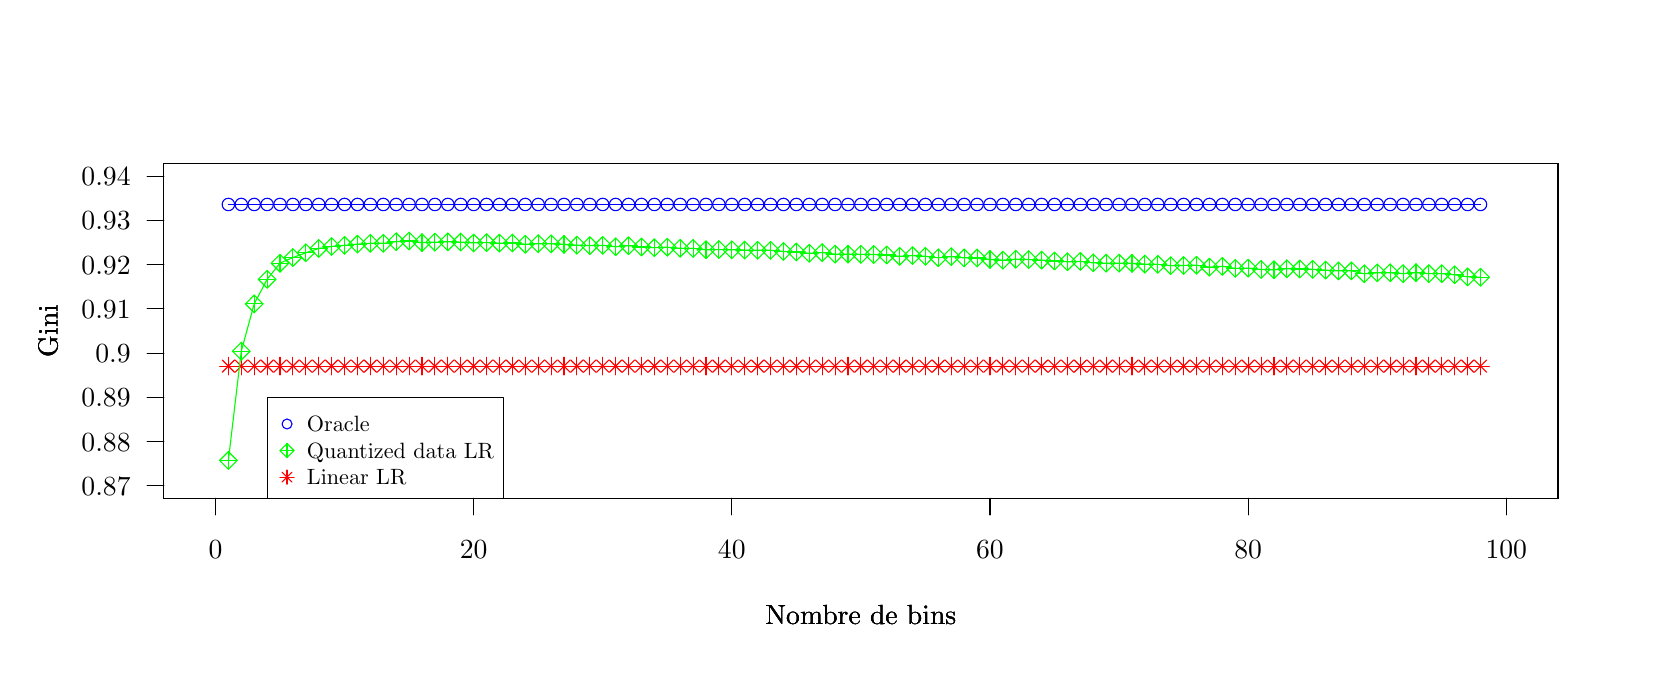
\begin{tikzpicture}[x=1pt,y=1pt]
\definecolor{fillColor}{RGB}{255,255,255}
\path[use as bounding box,fill=fillColor,fill opacity=0.00] (0,0) rectangle (578.16,231.26);
\begin{scope}
\path[clip] ( 49.20, 61.20) rectangle (552.96,182.06);
\definecolor{drawColor}{RGB}{255,0,0}

\path[draw=drawColor,line width= 0.4pt,line join=round,line cap=round] ( 72.52,108.96) --
	( 77.19,108.96) --
	( 81.85,108.96) --
	( 86.52,108.96) --
	( 91.18,108.96) --
	( 95.84,108.96) --
	(100.51,108.96) --
	(105.17,108.96) --
	(109.84,108.96) --
	(114.50,108.96) --
	(119.17,108.96) --
	(123.83,108.96) --
	(128.50,108.96) --
	(133.16,108.96) --
	(137.82,108.96) --
	(142.49,108.96) --
	(147.15,108.96) --
	(151.82,108.96) --
	(156.48,108.96) --
	(161.15,108.96) --
	(165.81,108.96) --
	(170.48,108.96) --
	(175.14,108.96) --
	(179.80,108.96) --
	(184.47,108.96) --
	(189.13,108.96) --
	(193.80,108.96) --
	(198.46,108.96) --
	(203.13,108.96) --
	(207.79,108.96) --
	(212.46,108.96) --
	(217.12,108.96) --
	(221.78,108.96) --
	(226.45,108.96) --
	(231.11,108.96) --
	(235.78,108.96) --
	(240.44,108.96) --
	(245.11,108.96) --
	(249.77,108.96) --
	(254.44,108.96) --
	(259.10,108.96) --
	(263.76,108.96) --
	(268.43,108.96) --
	(273.09,108.96) --
	(277.76,108.96) --
	(282.42,108.96) --
	(287.09,108.96) --
	(291.75,108.96) --
	(296.42,108.96) --
	(301.08,108.96) --
	(305.74,108.96) --
	(310.41,108.96) --
	(315.07,108.96) --
	(319.74,108.96) --
	(324.40,108.96) --
	(329.07,108.96) --
	(333.73,108.96) --
	(338.40,108.96) --
	(343.06,108.96) --
	(347.72,108.96) --
	(352.39,108.96) --
	(357.05,108.96) --
	(361.72,108.96) --
	(366.38,108.96) --
	(371.05,108.96) --
	(375.71,108.96) --
	(380.38,108.96) --
	(385.04,108.96) --
	(389.70,108.96) --
	(394.37,108.96) --
	(399.03,108.96) --
	(403.70,108.96) --
	(408.36,108.96) --
	(413.03,108.96) --
	(417.69,108.96) --
	(422.36,108.96) --
	(427.02,108.96) --
	(431.68,108.96) --
	(436.35,108.96) --
	(441.01,108.96) --
	(445.68,108.96) --
	(450.34,108.96) --
	(455.01,108.96) --
	(459.67,108.96) --
	(464.34,108.96) --
	(469.00,108.96) --
	(473.66,108.96) --
	(478.33,108.96) --
	(482.99,108.96) --
	(487.66,108.96) --
	(492.32,108.96) --
	(496.99,108.96) --
	(501.65,108.96) --
	(506.32,108.96) --
	(510.98,108.96) --
	(515.64,108.96) --
	(520.31,108.96) --
	(524.97,108.96);

\path[draw=drawColor,line width= 0.4pt,line join=round,line cap=round] ( 70.27,106.71) -- ( 74.77,111.21);

\path[draw=drawColor,line width= 0.4pt,line join=round,line cap=round] ( 70.27,111.21) -- ( 74.77,106.71);

\path[draw=drawColor,line width= 0.4pt,line join=round,line cap=round] ( 69.34,108.96) -- ( 75.70,108.96);

\path[draw=drawColor,line width= 0.4pt,line join=round,line cap=round] ( 72.52,105.78) -- ( 72.52,112.15);

\path[draw=drawColor,line width= 0.4pt,line join=round,line cap=round] ( 74.94,106.71) -- ( 79.44,111.21);

\path[draw=drawColor,line width= 0.4pt,line join=round,line cap=round] ( 74.94,111.21) -- ( 79.44,106.71);

\path[draw=drawColor,line width= 0.4pt,line join=round,line cap=round] ( 74.00,108.96) -- ( 80.37,108.96);

\path[draw=drawColor,line width= 0.4pt,line join=round,line cap=round] ( 77.19,105.78) -- ( 77.19,112.15);

\path[draw=drawColor,line width= 0.4pt,line join=round,line cap=round] ( 79.60,106.71) -- ( 84.10,111.21);

\path[draw=drawColor,line width= 0.4pt,line join=round,line cap=round] ( 79.60,111.21) -- ( 84.10,106.71);

\path[draw=drawColor,line width= 0.4pt,line join=round,line cap=round] ( 78.67,108.96) -- ( 85.03,108.96);

\path[draw=drawColor,line width= 0.4pt,line join=round,line cap=round] ( 81.85,105.78) -- ( 81.85,112.15);

\path[draw=drawColor,line width= 0.4pt,line join=round,line cap=round] ( 84.27,106.71) -- ( 88.77,111.21);

\path[draw=drawColor,line width= 0.4pt,line join=round,line cap=round] ( 84.27,111.21) -- ( 88.77,106.71);

\path[draw=drawColor,line width= 0.4pt,line join=round,line cap=round] ( 83.33,108.96) -- ( 89.70,108.96);

\path[draw=drawColor,line width= 0.4pt,line join=round,line cap=round] ( 86.52,105.78) -- ( 86.52,112.15);

\path[draw=drawColor,line width= 0.4pt,line join=round,line cap=round] ( 88.93,106.71) -- ( 93.43,111.21);

\path[draw=drawColor,line width= 0.4pt,line join=round,line cap=round] ( 88.93,111.21) -- ( 93.43,106.71);

\path[draw=drawColor,line width= 0.4pt,line join=round,line cap=round] ( 88.00,108.96) -- ( 94.36,108.96);

\path[draw=drawColor,line width= 0.4pt,line join=round,line cap=round] ( 91.18,105.78) -- ( 91.18,112.15);

\path[draw=drawColor,line width= 0.4pt,line join=round,line cap=round] ( 93.59,106.71) -- ( 98.09,111.21);

\path[draw=drawColor,line width= 0.4pt,line join=round,line cap=round] ( 93.59,111.21) -- ( 98.09,106.71);

\path[draw=drawColor,line width= 0.4pt,line join=round,line cap=round] ( 92.66,108.96) -- ( 99.03,108.96);

\path[draw=drawColor,line width= 0.4pt,line join=round,line cap=round] ( 95.84,105.78) -- ( 95.84,112.15);

\path[draw=drawColor,line width= 0.4pt,line join=round,line cap=round] ( 98.26,106.71) -- (102.76,111.21);

\path[draw=drawColor,line width= 0.4pt,line join=round,line cap=round] ( 98.26,111.21) -- (102.76,106.71);

\path[draw=drawColor,line width= 0.4pt,line join=round,line cap=round] ( 97.33,108.96) -- (103.69,108.96);

\path[draw=drawColor,line width= 0.4pt,line join=round,line cap=round] (100.51,105.78) -- (100.51,112.15);

\path[draw=drawColor,line width= 0.4pt,line join=round,line cap=round] (102.92,106.71) -- (107.42,111.21);

\path[draw=drawColor,line width= 0.4pt,line join=round,line cap=round] (102.92,111.21) -- (107.42,106.71);

\path[draw=drawColor,line width= 0.4pt,line join=round,line cap=round] (101.99,108.96) -- (108.36,108.96);

\path[draw=drawColor,line width= 0.4pt,line join=round,line cap=round] (105.17,105.78) -- (105.17,112.15);

\path[draw=drawColor,line width= 0.4pt,line join=round,line cap=round] (107.59,106.71) -- (112.09,111.21);

\path[draw=drawColor,line width= 0.4pt,line join=round,line cap=round] (107.59,111.21) -- (112.09,106.71);

\path[draw=drawColor,line width= 0.4pt,line join=round,line cap=round] (106.66,108.96) -- (113.02,108.96);

\path[draw=drawColor,line width= 0.4pt,line join=round,line cap=round] (109.84,105.78) -- (109.84,112.15);

\path[draw=drawColor,line width= 0.4pt,line join=round,line cap=round] (112.25,106.71) -- (116.75,111.21);

\path[draw=drawColor,line width= 0.4pt,line join=round,line cap=round] (112.25,111.21) -- (116.75,106.71);

\path[draw=drawColor,line width= 0.4pt,line join=round,line cap=round] (111.32,108.96) -- (117.68,108.96);

\path[draw=drawColor,line width= 0.4pt,line join=round,line cap=round] (114.50,105.78) -- (114.50,112.15);

\path[draw=drawColor,line width= 0.4pt,line join=round,line cap=round] (116.92,106.71) -- (121.42,111.21);

\path[draw=drawColor,line width= 0.4pt,line join=round,line cap=round] (116.92,111.21) -- (121.42,106.71);

\path[draw=drawColor,line width= 0.4pt,line join=round,line cap=round] (115.98,108.96) -- (122.35,108.96);

\path[draw=drawColor,line width= 0.4pt,line join=round,line cap=round] (119.17,105.78) -- (119.17,112.15);

\path[draw=drawColor,line width= 0.4pt,line join=round,line cap=round] (121.58,106.71) -- (126.08,111.21);

\path[draw=drawColor,line width= 0.4pt,line join=round,line cap=round] (121.58,111.21) -- (126.08,106.71);

\path[draw=drawColor,line width= 0.4pt,line join=round,line cap=round] (120.65,108.96) -- (127.01,108.96);

\path[draw=drawColor,line width= 0.4pt,line join=round,line cap=round] (123.83,105.78) -- (123.83,112.15);

\path[draw=drawColor,line width= 0.4pt,line join=round,line cap=round] (126.25,106.71) -- (130.75,111.21);

\path[draw=drawColor,line width= 0.4pt,line join=round,line cap=round] (126.25,111.21) -- (130.75,106.71);

\path[draw=drawColor,line width= 0.4pt,line join=round,line cap=round] (125.31,108.96) -- (131.68,108.96);

\path[draw=drawColor,line width= 0.4pt,line join=round,line cap=round] (128.50,105.78) -- (128.50,112.15);

\path[draw=drawColor,line width= 0.4pt,line join=round,line cap=round] (130.91,106.71) -- (135.41,111.21);

\path[draw=drawColor,line width= 0.4pt,line join=round,line cap=round] (130.91,111.21) -- (135.41,106.71);

\path[draw=drawColor,line width= 0.4pt,line join=round,line cap=round] (129.98,108.96) -- (136.34,108.96);

\path[draw=drawColor,line width= 0.4pt,line join=round,line cap=round] (133.16,105.78) -- (133.16,112.15);

\path[draw=drawColor,line width= 0.4pt,line join=round,line cap=round] (135.57,106.71) -- (140.07,111.21);

\path[draw=drawColor,line width= 0.4pt,line join=round,line cap=round] (135.57,111.21) -- (140.07,106.71);

\path[draw=drawColor,line width= 0.4pt,line join=round,line cap=round] (134.64,108.96) -- (141.01,108.96);

\path[draw=drawColor,line width= 0.4pt,line join=round,line cap=round] (137.82,105.78) -- (137.82,112.15);

\path[draw=drawColor,line width= 0.4pt,line join=round,line cap=round] (140.24,106.71) -- (144.74,111.21);

\path[draw=drawColor,line width= 0.4pt,line join=round,line cap=round] (140.24,111.21) -- (144.74,106.71);

\path[draw=drawColor,line width= 0.4pt,line join=round,line cap=round] (139.31,108.96) -- (145.67,108.96);

\path[draw=drawColor,line width= 0.4pt,line join=round,line cap=round] (142.49,105.78) -- (142.49,112.15);

\path[draw=drawColor,line width= 0.4pt,line join=round,line cap=round] (144.90,106.71) -- (149.40,111.21);

\path[draw=drawColor,line width= 0.4pt,line join=round,line cap=round] (144.90,111.21) -- (149.40,106.71);

\path[draw=drawColor,line width= 0.4pt,line join=round,line cap=round] (143.97,108.96) -- (150.34,108.96);

\path[draw=drawColor,line width= 0.4pt,line join=round,line cap=round] (147.15,105.78) -- (147.15,112.15);

\path[draw=drawColor,line width= 0.4pt,line join=round,line cap=round] (149.57,106.71) -- (154.07,111.21);

\path[draw=drawColor,line width= 0.4pt,line join=round,line cap=round] (149.57,111.21) -- (154.07,106.71);

\path[draw=drawColor,line width= 0.4pt,line join=round,line cap=round] (148.64,108.96) -- (155.00,108.96);

\path[draw=drawColor,line width= 0.4pt,line join=round,line cap=round] (151.82,105.78) -- (151.82,112.15);

\path[draw=drawColor,line width= 0.4pt,line join=round,line cap=round] (154.23,106.71) -- (158.73,111.21);

\path[draw=drawColor,line width= 0.4pt,line join=round,line cap=round] (154.23,111.21) -- (158.73,106.71);

\path[draw=drawColor,line width= 0.4pt,line join=round,line cap=round] (153.30,108.96) -- (159.66,108.96);

\path[draw=drawColor,line width= 0.4pt,line join=round,line cap=round] (156.48,105.78) -- (156.48,112.15);

\path[draw=drawColor,line width= 0.4pt,line join=round,line cap=round] (158.90,106.71) -- (163.40,111.21);

\path[draw=drawColor,line width= 0.4pt,line join=round,line cap=round] (158.90,111.21) -- (163.40,106.71);

\path[draw=drawColor,line width= 0.4pt,line join=round,line cap=round] (157.96,108.96) -- (164.33,108.96);

\path[draw=drawColor,line width= 0.4pt,line join=round,line cap=round] (161.15,105.78) -- (161.15,112.15);

\path[draw=drawColor,line width= 0.4pt,line join=round,line cap=round] (163.56,106.71) -- (168.06,111.21);

\path[draw=drawColor,line width= 0.4pt,line join=round,line cap=round] (163.56,111.21) -- (168.06,106.71);

\path[draw=drawColor,line width= 0.4pt,line join=round,line cap=round] (162.63,108.96) -- (168.99,108.96);

\path[draw=drawColor,line width= 0.4pt,line join=round,line cap=round] (165.81,105.78) -- (165.81,112.15);

\path[draw=drawColor,line width= 0.4pt,line join=round,line cap=round] (168.23,106.71) -- (172.73,111.21);

\path[draw=drawColor,line width= 0.4pt,line join=round,line cap=round] (168.23,111.21) -- (172.73,106.71);

\path[draw=drawColor,line width= 0.4pt,line join=round,line cap=round] (167.29,108.96) -- (173.66,108.96);

\path[draw=drawColor,line width= 0.4pt,line join=round,line cap=round] (170.48,105.78) -- (170.48,112.15);

\path[draw=drawColor,line width= 0.4pt,line join=round,line cap=round] (172.89,106.71) -- (177.39,111.21);

\path[draw=drawColor,line width= 0.4pt,line join=round,line cap=round] (172.89,111.21) -- (177.39,106.71);

\path[draw=drawColor,line width= 0.4pt,line join=round,line cap=round] (171.96,108.96) -- (178.32,108.96);

\path[draw=drawColor,line width= 0.4pt,line join=round,line cap=round] (175.14,105.78) -- (175.14,112.15);

\path[draw=drawColor,line width= 0.4pt,line join=round,line cap=round] (177.55,106.71) -- (182.05,111.21);

\path[draw=drawColor,line width= 0.4pt,line join=round,line cap=round] (177.55,111.21) -- (182.05,106.71);

\path[draw=drawColor,line width= 0.4pt,line join=round,line cap=round] (176.62,108.96) -- (182.99,108.96);

\path[draw=drawColor,line width= 0.4pt,line join=round,line cap=round] (179.80,105.78) -- (179.80,112.15);

\path[draw=drawColor,line width= 0.4pt,line join=round,line cap=round] (182.22,106.71) -- (186.72,111.21);

\path[draw=drawColor,line width= 0.4pt,line join=round,line cap=round] (182.22,111.21) -- (186.72,106.71);

\path[draw=drawColor,line width= 0.4pt,line join=round,line cap=round] (181.29,108.96) -- (187.65,108.96);

\path[draw=drawColor,line width= 0.4pt,line join=round,line cap=round] (184.47,105.78) -- (184.47,112.15);

\path[draw=drawColor,line width= 0.4pt,line join=round,line cap=round] (186.88,106.71) -- (191.38,111.21);

\path[draw=drawColor,line width= 0.4pt,line join=round,line cap=round] (186.88,111.21) -- (191.38,106.71);

\path[draw=drawColor,line width= 0.4pt,line join=round,line cap=round] (185.95,108.96) -- (192.32,108.96);

\path[draw=drawColor,line width= 0.4pt,line join=round,line cap=round] (189.13,105.78) -- (189.13,112.15);

\path[draw=drawColor,line width= 0.4pt,line join=round,line cap=round] (191.55,106.71) -- (196.05,111.21);

\path[draw=drawColor,line width= 0.4pt,line join=round,line cap=round] (191.55,111.21) -- (196.05,106.71);

\path[draw=drawColor,line width= 0.4pt,line join=round,line cap=round] (190.62,108.96) -- (196.98,108.96);

\path[draw=drawColor,line width= 0.4pt,line join=round,line cap=round] (193.80,105.78) -- (193.80,112.15);

\path[draw=drawColor,line width= 0.4pt,line join=round,line cap=round] (196.21,106.71) -- (200.71,111.21);

\path[draw=drawColor,line width= 0.4pt,line join=round,line cap=round] (196.21,111.21) -- (200.71,106.71);

\path[draw=drawColor,line width= 0.4pt,line join=round,line cap=round] (195.28,108.96) -- (201.64,108.96);

\path[draw=drawColor,line width= 0.4pt,line join=round,line cap=round] (198.46,105.78) -- (198.46,112.15);

\path[draw=drawColor,line width= 0.4pt,line join=round,line cap=round] (200.88,106.71) -- (205.38,111.21);

\path[draw=drawColor,line width= 0.4pt,line join=round,line cap=round] (200.88,111.21) -- (205.38,106.71);

\path[draw=drawColor,line width= 0.4pt,line join=round,line cap=round] (199.94,108.96) -- (206.31,108.96);

\path[draw=drawColor,line width= 0.4pt,line join=round,line cap=round] (203.13,105.78) -- (203.13,112.15);

\path[draw=drawColor,line width= 0.4pt,line join=round,line cap=round] (205.54,106.71) -- (210.04,111.21);

\path[draw=drawColor,line width= 0.4pt,line join=round,line cap=round] (205.54,111.21) -- (210.04,106.71);

\path[draw=drawColor,line width= 0.4pt,line join=round,line cap=round] (204.61,108.96) -- (210.97,108.96);

\path[draw=drawColor,line width= 0.4pt,line join=round,line cap=round] (207.79,105.78) -- (207.79,112.15);

\path[draw=drawColor,line width= 0.4pt,line join=round,line cap=round] (210.21,106.71) -- (214.71,111.21);

\path[draw=drawColor,line width= 0.4pt,line join=round,line cap=round] (210.21,111.21) -- (214.71,106.71);

\path[draw=drawColor,line width= 0.4pt,line join=round,line cap=round] (209.27,108.96) -- (215.64,108.96);

\path[draw=drawColor,line width= 0.4pt,line join=round,line cap=round] (212.46,105.78) -- (212.46,112.15);

\path[draw=drawColor,line width= 0.4pt,line join=round,line cap=round] (214.87,106.71) -- (219.37,111.21);

\path[draw=drawColor,line width= 0.4pt,line join=round,line cap=round] (214.87,111.21) -- (219.37,106.71);

\path[draw=drawColor,line width= 0.4pt,line join=round,line cap=round] (213.94,108.96) -- (220.30,108.96);

\path[draw=drawColor,line width= 0.4pt,line join=round,line cap=round] (217.12,105.78) -- (217.12,112.15);

\path[draw=drawColor,line width= 0.4pt,line join=round,line cap=round] (219.53,106.71) -- (224.03,111.21);

\path[draw=drawColor,line width= 0.4pt,line join=round,line cap=round] (219.53,111.21) -- (224.03,106.71);

\path[draw=drawColor,line width= 0.4pt,line join=round,line cap=round] (218.60,108.96) -- (224.97,108.96);

\path[draw=drawColor,line width= 0.4pt,line join=round,line cap=round] (221.78,105.78) -- (221.78,112.15);

\path[draw=drawColor,line width= 0.4pt,line join=round,line cap=round] (224.20,106.71) -- (228.70,111.21);

\path[draw=drawColor,line width= 0.4pt,line join=round,line cap=round] (224.20,111.21) -- (228.70,106.71);

\path[draw=drawColor,line width= 0.4pt,line join=round,line cap=round] (223.27,108.96) -- (229.63,108.96);

\path[draw=drawColor,line width= 0.4pt,line join=round,line cap=round] (226.45,105.78) -- (226.45,112.15);

\path[draw=drawColor,line width= 0.4pt,line join=round,line cap=round] (228.86,106.71) -- (233.36,111.21);

\path[draw=drawColor,line width= 0.4pt,line join=round,line cap=round] (228.86,111.21) -- (233.36,106.71);

\path[draw=drawColor,line width= 0.4pt,line join=round,line cap=round] (227.93,108.96) -- (234.30,108.96);

\path[draw=drawColor,line width= 0.4pt,line join=round,line cap=round] (231.11,105.78) -- (231.11,112.15);

\path[draw=drawColor,line width= 0.4pt,line join=round,line cap=round] (233.53,106.71) -- (238.03,111.21);

\path[draw=drawColor,line width= 0.4pt,line join=round,line cap=round] (233.53,111.21) -- (238.03,106.71);

\path[draw=drawColor,line width= 0.4pt,line join=round,line cap=round] (232.60,108.96) -- (238.96,108.96);

\path[draw=drawColor,line width= 0.4pt,line join=round,line cap=round] (235.78,105.78) -- (235.78,112.15);

\path[draw=drawColor,line width= 0.4pt,line join=round,line cap=round] (238.19,106.71) -- (242.69,111.21);

\path[draw=drawColor,line width= 0.4pt,line join=round,line cap=round] (238.19,111.21) -- (242.69,106.71);

\path[draw=drawColor,line width= 0.4pt,line join=round,line cap=round] (237.26,108.96) -- (243.62,108.96);

\path[draw=drawColor,line width= 0.4pt,line join=round,line cap=round] (240.44,105.78) -- (240.44,112.15);

\path[draw=drawColor,line width= 0.4pt,line join=round,line cap=round] (242.86,106.71) -- (247.36,111.21);

\path[draw=drawColor,line width= 0.4pt,line join=round,line cap=round] (242.86,111.21) -- (247.36,106.71);

\path[draw=drawColor,line width= 0.4pt,line join=round,line cap=round] (241.92,108.96) -- (248.29,108.96);

\path[draw=drawColor,line width= 0.4pt,line join=round,line cap=round] (245.11,105.78) -- (245.11,112.15);

\path[draw=drawColor,line width= 0.4pt,line join=round,line cap=round] (247.52,106.71) -- (252.02,111.21);

\path[draw=drawColor,line width= 0.4pt,line join=round,line cap=round] (247.52,111.21) -- (252.02,106.71);

\path[draw=drawColor,line width= 0.4pt,line join=round,line cap=round] (246.59,108.96) -- (252.95,108.96);

\path[draw=drawColor,line width= 0.4pt,line join=round,line cap=round] (249.77,105.78) -- (249.77,112.15);

\path[draw=drawColor,line width= 0.4pt,line join=round,line cap=round] (252.19,106.71) -- (256.69,111.21);

\path[draw=drawColor,line width= 0.4pt,line join=round,line cap=round] (252.19,111.21) -- (256.69,106.71);

\path[draw=drawColor,line width= 0.4pt,line join=round,line cap=round] (251.25,108.96) -- (257.62,108.96);

\path[draw=drawColor,line width= 0.4pt,line join=round,line cap=round] (254.44,105.78) -- (254.44,112.15);

\path[draw=drawColor,line width= 0.4pt,line join=round,line cap=round] (256.85,106.71) -- (261.35,111.21);

\path[draw=drawColor,line width= 0.4pt,line join=round,line cap=round] (256.85,111.21) -- (261.35,106.71);

\path[draw=drawColor,line width= 0.4pt,line join=round,line cap=round] (255.92,108.96) -- (262.28,108.96);

\path[draw=drawColor,line width= 0.4pt,line join=round,line cap=round] (259.10,105.78) -- (259.10,112.15);

\path[draw=drawColor,line width= 0.4pt,line join=round,line cap=round] (261.51,106.71) -- (266.01,111.21);

\path[draw=drawColor,line width= 0.4pt,line join=round,line cap=round] (261.51,111.21) -- (266.01,106.71);

\path[draw=drawColor,line width= 0.4pt,line join=round,line cap=round] (260.58,108.96) -- (266.95,108.96);

\path[draw=drawColor,line width= 0.4pt,line join=round,line cap=round] (263.76,105.78) -- (263.76,112.15);

\path[draw=drawColor,line width= 0.4pt,line join=round,line cap=round] (266.18,106.71) -- (270.68,111.21);

\path[draw=drawColor,line width= 0.4pt,line join=round,line cap=round] (266.18,111.21) -- (270.68,106.71);

\path[draw=drawColor,line width= 0.4pt,line join=round,line cap=round] (265.25,108.96) -- (271.61,108.96);

\path[draw=drawColor,line width= 0.4pt,line join=round,line cap=round] (268.43,105.78) -- (268.43,112.15);

\path[draw=drawColor,line width= 0.4pt,line join=round,line cap=round] (270.84,106.71) -- (275.34,111.21);

\path[draw=drawColor,line width= 0.4pt,line join=round,line cap=round] (270.84,111.21) -- (275.34,106.71);

\path[draw=drawColor,line width= 0.4pt,line join=round,line cap=round] (269.91,108.96) -- (276.28,108.96);

\path[draw=drawColor,line width= 0.4pt,line join=round,line cap=round] (273.09,105.78) -- (273.09,112.15);

\path[draw=drawColor,line width= 0.4pt,line join=round,line cap=round] (275.51,106.71) -- (280.01,111.21);

\path[draw=drawColor,line width= 0.4pt,line join=round,line cap=round] (275.51,111.21) -- (280.01,106.71);

\path[draw=drawColor,line width= 0.4pt,line join=round,line cap=round] (274.58,108.96) -- (280.94,108.96);

\path[draw=drawColor,line width= 0.4pt,line join=round,line cap=round] (277.76,105.78) -- (277.76,112.15);

\path[draw=drawColor,line width= 0.4pt,line join=round,line cap=round] (280.17,106.71) -- (284.67,111.21);

\path[draw=drawColor,line width= 0.4pt,line join=round,line cap=round] (280.17,111.21) -- (284.67,106.71);

\path[draw=drawColor,line width= 0.4pt,line join=round,line cap=round] (279.24,108.96) -- (285.60,108.96);

\path[draw=drawColor,line width= 0.4pt,line join=round,line cap=round] (282.42,105.78) -- (282.42,112.15);

\path[draw=drawColor,line width= 0.4pt,line join=round,line cap=round] (284.84,106.71) -- (289.34,111.21);

\path[draw=drawColor,line width= 0.4pt,line join=round,line cap=round] (284.84,111.21) -- (289.34,106.71);

\path[draw=drawColor,line width= 0.4pt,line join=round,line cap=round] (283.90,108.96) -- (290.27,108.96);

\path[draw=drawColor,line width= 0.4pt,line join=round,line cap=round] (287.09,105.78) -- (287.09,112.15);

\path[draw=drawColor,line width= 0.4pt,line join=round,line cap=round] (289.50,106.71) -- (294.00,111.21);

\path[draw=drawColor,line width= 0.4pt,line join=round,line cap=round] (289.50,111.21) -- (294.00,106.71);

\path[draw=drawColor,line width= 0.4pt,line join=round,line cap=round] (288.57,108.96) -- (294.93,108.96);

\path[draw=drawColor,line width= 0.4pt,line join=round,line cap=round] (291.75,105.78) -- (291.75,112.15);

\path[draw=drawColor,line width= 0.4pt,line join=round,line cap=round] (294.17,106.71) -- (298.67,111.21);

\path[draw=drawColor,line width= 0.4pt,line join=round,line cap=round] (294.17,111.21) -- (298.67,106.71);

\path[draw=drawColor,line width= 0.4pt,line join=round,line cap=round] (293.23,108.96) -- (299.60,108.96);

\path[draw=drawColor,line width= 0.4pt,line join=round,line cap=round] (296.42,105.78) -- (296.42,112.15);

\path[draw=drawColor,line width= 0.4pt,line join=round,line cap=round] (298.83,106.71) -- (303.33,111.21);

\path[draw=drawColor,line width= 0.4pt,line join=round,line cap=round] (298.83,111.21) -- (303.33,106.71);

\path[draw=drawColor,line width= 0.4pt,line join=round,line cap=round] (297.90,108.96) -- (304.26,108.96);

\path[draw=drawColor,line width= 0.4pt,line join=round,line cap=round] (301.08,105.78) -- (301.08,112.15);

\path[draw=drawColor,line width= 0.4pt,line join=round,line cap=round] (303.49,106.71) -- (307.99,111.21);

\path[draw=drawColor,line width= 0.4pt,line join=round,line cap=round] (303.49,111.21) -- (307.99,106.71);

\path[draw=drawColor,line width= 0.4pt,line join=round,line cap=round] (302.56,108.96) -- (308.93,108.96);

\path[draw=drawColor,line width= 0.4pt,line join=round,line cap=round] (305.74,105.78) -- (305.74,112.15);

\path[draw=drawColor,line width= 0.4pt,line join=round,line cap=round] (308.16,106.71) -- (312.66,111.21);

\path[draw=drawColor,line width= 0.4pt,line join=round,line cap=round] (308.16,111.21) -- (312.66,106.71);

\path[draw=drawColor,line width= 0.4pt,line join=round,line cap=round] (307.23,108.96) -- (313.59,108.96);

\path[draw=drawColor,line width= 0.4pt,line join=round,line cap=round] (310.41,105.78) -- (310.41,112.15);

\path[draw=drawColor,line width= 0.4pt,line join=round,line cap=round] (312.82,106.71) -- (317.32,111.21);

\path[draw=drawColor,line width= 0.4pt,line join=round,line cap=round] (312.82,111.21) -- (317.32,106.71);

\path[draw=drawColor,line width= 0.4pt,line join=round,line cap=round] (311.89,108.96) -- (318.26,108.96);

\path[draw=drawColor,line width= 0.4pt,line join=round,line cap=round] (315.07,105.78) -- (315.07,112.15);

\path[draw=drawColor,line width= 0.4pt,line join=round,line cap=round] (317.49,106.71) -- (321.99,111.21);

\path[draw=drawColor,line width= 0.4pt,line join=round,line cap=round] (317.49,111.21) -- (321.99,106.71);

\path[draw=drawColor,line width= 0.4pt,line join=round,line cap=round] (316.56,108.96) -- (322.92,108.96);

\path[draw=drawColor,line width= 0.4pt,line join=round,line cap=round] (319.74,105.78) -- (319.74,112.15);

\path[draw=drawColor,line width= 0.4pt,line join=round,line cap=round] (322.15,106.71) -- (326.65,111.21);

\path[draw=drawColor,line width= 0.4pt,line join=round,line cap=round] (322.15,111.21) -- (326.65,106.71);

\path[draw=drawColor,line width= 0.4pt,line join=round,line cap=round] (321.22,108.96) -- (327.58,108.96);

\path[draw=drawColor,line width= 0.4pt,line join=round,line cap=round] (324.40,105.78) -- (324.40,112.15);

\path[draw=drawColor,line width= 0.4pt,line join=round,line cap=round] (326.82,106.71) -- (331.32,111.21);

\path[draw=drawColor,line width= 0.4pt,line join=round,line cap=round] (326.82,111.21) -- (331.32,106.71);

\path[draw=drawColor,line width= 0.4pt,line join=round,line cap=round] (325.88,108.96) -- (332.25,108.96);

\path[draw=drawColor,line width= 0.4pt,line join=round,line cap=round] (329.07,105.78) -- (329.07,112.15);

\path[draw=drawColor,line width= 0.4pt,line join=round,line cap=round] (331.48,106.71) -- (335.98,111.21);

\path[draw=drawColor,line width= 0.4pt,line join=round,line cap=round] (331.48,111.21) -- (335.98,106.71);

\path[draw=drawColor,line width= 0.4pt,line join=round,line cap=round] (330.55,108.96) -- (336.91,108.96);

\path[draw=drawColor,line width= 0.4pt,line join=round,line cap=round] (333.73,105.78) -- (333.73,112.15);

\path[draw=drawColor,line width= 0.4pt,line join=round,line cap=round] (336.15,106.71) -- (340.65,111.21);

\path[draw=drawColor,line width= 0.4pt,line join=round,line cap=round] (336.15,111.21) -- (340.65,106.71);

\path[draw=drawColor,line width= 0.4pt,line join=round,line cap=round] (335.21,108.96) -- (341.58,108.96);

\path[draw=drawColor,line width= 0.4pt,line join=round,line cap=round] (338.40,105.78) -- (338.40,112.15);

\path[draw=drawColor,line width= 0.4pt,line join=round,line cap=round] (340.81,106.71) -- (345.31,111.21);

\path[draw=drawColor,line width= 0.4pt,line join=round,line cap=round] (340.81,111.21) -- (345.31,106.71);

\path[draw=drawColor,line width= 0.4pt,line join=round,line cap=round] (339.88,108.96) -- (346.24,108.96);

\path[draw=drawColor,line width= 0.4pt,line join=round,line cap=round] (343.06,105.78) -- (343.06,112.15);

\path[draw=drawColor,line width= 0.4pt,line join=round,line cap=round] (345.47,106.71) -- (349.97,111.21);

\path[draw=drawColor,line width= 0.4pt,line join=round,line cap=round] (345.47,111.21) -- (349.97,106.71);

\path[draw=drawColor,line width= 0.4pt,line join=round,line cap=round] (344.54,108.96) -- (350.91,108.96);

\path[draw=drawColor,line width= 0.4pt,line join=round,line cap=round] (347.72,105.78) -- (347.72,112.15);

\path[draw=drawColor,line width= 0.4pt,line join=round,line cap=round] (350.14,106.71) -- (354.64,111.21);

\path[draw=drawColor,line width= 0.4pt,line join=round,line cap=round] (350.14,111.21) -- (354.64,106.71);

\path[draw=drawColor,line width= 0.4pt,line join=round,line cap=round] (349.21,108.96) -- (355.57,108.96);

\path[draw=drawColor,line width= 0.4pt,line join=round,line cap=round] (352.39,105.78) -- (352.39,112.15);

\path[draw=drawColor,line width= 0.4pt,line join=round,line cap=round] (354.80,106.71) -- (359.30,111.21);

\path[draw=drawColor,line width= 0.4pt,line join=round,line cap=round] (354.80,111.21) -- (359.30,106.71);

\path[draw=drawColor,line width= 0.4pt,line join=round,line cap=round] (353.87,108.96) -- (360.24,108.96);

\path[draw=drawColor,line width= 0.4pt,line join=round,line cap=round] (357.05,105.78) -- (357.05,112.15);

\path[draw=drawColor,line width= 0.4pt,line join=round,line cap=round] (359.47,106.71) -- (363.97,111.21);

\path[draw=drawColor,line width= 0.4pt,line join=round,line cap=round] (359.47,111.21) -- (363.97,106.71);

\path[draw=drawColor,line width= 0.4pt,line join=round,line cap=round] (358.54,108.96) -- (364.90,108.96);

\path[draw=drawColor,line width= 0.4pt,line join=round,line cap=round] (361.72,105.78) -- (361.72,112.15);

\path[draw=drawColor,line width= 0.4pt,line join=round,line cap=round] (364.13,106.71) -- (368.63,111.21);

\path[draw=drawColor,line width= 0.4pt,line join=round,line cap=round] (364.13,111.21) -- (368.63,106.71);

\path[draw=drawColor,line width= 0.4pt,line join=round,line cap=round] (363.20,108.96) -- (369.56,108.96);

\path[draw=drawColor,line width= 0.4pt,line join=round,line cap=round] (366.38,105.78) -- (366.38,112.15);

\path[draw=drawColor,line width= 0.4pt,line join=round,line cap=round] (368.80,106.71) -- (373.30,111.21);

\path[draw=drawColor,line width= 0.4pt,line join=round,line cap=round] (368.80,111.21) -- (373.30,106.71);

\path[draw=drawColor,line width= 0.4pt,line join=round,line cap=round] (367.86,108.96) -- (374.23,108.96);

\path[draw=drawColor,line width= 0.4pt,line join=round,line cap=round] (371.05,105.78) -- (371.05,112.15);

\path[draw=drawColor,line width= 0.4pt,line join=round,line cap=round] (373.46,106.71) -- (377.96,111.21);

\path[draw=drawColor,line width= 0.4pt,line join=round,line cap=round] (373.46,111.21) -- (377.96,106.71);

\path[draw=drawColor,line width= 0.4pt,line join=round,line cap=round] (372.53,108.96) -- (378.89,108.96);

\path[draw=drawColor,line width= 0.4pt,line join=round,line cap=round] (375.71,105.78) -- (375.71,112.15);

\path[draw=drawColor,line width= 0.4pt,line join=round,line cap=round] (378.13,106.71) -- (382.63,111.21);

\path[draw=drawColor,line width= 0.4pt,line join=round,line cap=round] (378.13,111.21) -- (382.63,106.71);

\path[draw=drawColor,line width= 0.4pt,line join=round,line cap=round] (377.19,108.96) -- (383.56,108.96);

\path[draw=drawColor,line width= 0.4pt,line join=round,line cap=round] (380.38,105.78) -- (380.38,112.15);

\path[draw=drawColor,line width= 0.4pt,line join=round,line cap=round] (382.79,106.71) -- (387.29,111.21);

\path[draw=drawColor,line width= 0.4pt,line join=round,line cap=round] (382.79,111.21) -- (387.29,106.71);

\path[draw=drawColor,line width= 0.4pt,line join=round,line cap=round] (381.86,108.96) -- (388.22,108.96);

\path[draw=drawColor,line width= 0.4pt,line join=round,line cap=round] (385.04,105.78) -- (385.04,112.15);

\path[draw=drawColor,line width= 0.4pt,line join=round,line cap=round] (387.45,106.71) -- (391.95,111.21);

\path[draw=drawColor,line width= 0.4pt,line join=round,line cap=round] (387.45,111.21) -- (391.95,106.71);

\path[draw=drawColor,line width= 0.4pt,line join=round,line cap=round] (386.52,108.96) -- (392.89,108.96);

\path[draw=drawColor,line width= 0.4pt,line join=round,line cap=round] (389.70,105.78) -- (389.70,112.15);

\path[draw=drawColor,line width= 0.4pt,line join=round,line cap=round] (392.12,106.71) -- (396.62,111.21);

\path[draw=drawColor,line width= 0.4pt,line join=round,line cap=round] (392.12,111.21) -- (396.62,106.71);

\path[draw=drawColor,line width= 0.4pt,line join=round,line cap=round] (391.19,108.96) -- (397.55,108.96);

\path[draw=drawColor,line width= 0.4pt,line join=round,line cap=round] (394.37,105.78) -- (394.37,112.15);

\path[draw=drawColor,line width= 0.4pt,line join=round,line cap=round] (396.78,106.71) -- (401.28,111.21);

\path[draw=drawColor,line width= 0.4pt,line join=round,line cap=round] (396.78,111.21) -- (401.28,106.71);

\path[draw=drawColor,line width= 0.4pt,line join=round,line cap=round] (395.85,108.96) -- (402.22,108.96);

\path[draw=drawColor,line width= 0.4pt,line join=round,line cap=round] (399.03,105.78) -- (399.03,112.15);

\path[draw=drawColor,line width= 0.4pt,line join=round,line cap=round] (401.45,106.71) -- (405.95,111.21);

\path[draw=drawColor,line width= 0.4pt,line join=round,line cap=round] (401.45,111.21) -- (405.95,106.71);

\path[draw=drawColor,line width= 0.4pt,line join=round,line cap=round] (400.52,108.96) -- (406.88,108.96);

\path[draw=drawColor,line width= 0.4pt,line join=round,line cap=round] (403.70,105.78) -- (403.70,112.15);

\path[draw=drawColor,line width= 0.4pt,line join=round,line cap=round] (406.11,106.71) -- (410.61,111.21);

\path[draw=drawColor,line width= 0.4pt,line join=round,line cap=round] (406.11,111.21) -- (410.61,106.71);

\path[draw=drawColor,line width= 0.4pt,line join=round,line cap=round] (405.18,108.96) -- (411.54,108.96);

\path[draw=drawColor,line width= 0.4pt,line join=round,line cap=round] (408.36,105.78) -- (408.36,112.15);

\path[draw=drawColor,line width= 0.4pt,line join=round,line cap=round] (410.78,106.71) -- (415.28,111.21);

\path[draw=drawColor,line width= 0.4pt,line join=round,line cap=round] (410.78,111.21) -- (415.28,106.71);

\path[draw=drawColor,line width= 0.4pt,line join=round,line cap=round] (409.84,108.96) -- (416.21,108.96);

\path[draw=drawColor,line width= 0.4pt,line join=round,line cap=round] (413.03,105.78) -- (413.03,112.15);

\path[draw=drawColor,line width= 0.4pt,line join=round,line cap=round] (415.44,106.71) -- (419.94,111.21);

\path[draw=drawColor,line width= 0.4pt,line join=round,line cap=round] (415.44,111.21) -- (419.94,106.71);

\path[draw=drawColor,line width= 0.4pt,line join=round,line cap=round] (414.51,108.96) -- (420.87,108.96);

\path[draw=drawColor,line width= 0.4pt,line join=round,line cap=round] (417.69,105.78) -- (417.69,112.15);

\path[draw=drawColor,line width= 0.4pt,line join=round,line cap=round] (420.11,106.71) -- (424.61,111.21);

\path[draw=drawColor,line width= 0.4pt,line join=round,line cap=round] (420.11,111.21) -- (424.61,106.71);

\path[draw=drawColor,line width= 0.4pt,line join=round,line cap=round] (419.17,108.96) -- (425.54,108.96);

\path[draw=drawColor,line width= 0.4pt,line join=round,line cap=round] (422.36,105.78) -- (422.36,112.15);

\path[draw=drawColor,line width= 0.4pt,line join=round,line cap=round] (424.77,106.71) -- (429.27,111.21);

\path[draw=drawColor,line width= 0.4pt,line join=round,line cap=round] (424.77,111.21) -- (429.27,106.71);

\path[draw=drawColor,line width= 0.4pt,line join=round,line cap=round] (423.84,108.96) -- (430.20,108.96);

\path[draw=drawColor,line width= 0.4pt,line join=round,line cap=round] (427.02,105.78) -- (427.02,112.15);

\path[draw=drawColor,line width= 0.4pt,line join=round,line cap=round] (429.43,106.71) -- (433.93,111.21);

\path[draw=drawColor,line width= 0.4pt,line join=round,line cap=round] (429.43,111.21) -- (433.93,106.71);

\path[draw=drawColor,line width= 0.4pt,line join=round,line cap=round] (428.50,108.96) -- (434.87,108.96);

\path[draw=drawColor,line width= 0.4pt,line join=round,line cap=round] (431.68,105.78) -- (431.68,112.15);

\path[draw=drawColor,line width= 0.4pt,line join=round,line cap=round] (434.10,106.71) -- (438.60,111.21);

\path[draw=drawColor,line width= 0.4pt,line join=round,line cap=round] (434.10,111.21) -- (438.60,106.71);

\path[draw=drawColor,line width= 0.4pt,line join=round,line cap=round] (433.17,108.96) -- (439.53,108.96);

\path[draw=drawColor,line width= 0.4pt,line join=round,line cap=round] (436.35,105.78) -- (436.35,112.15);

\path[draw=drawColor,line width= 0.4pt,line join=round,line cap=round] (438.76,106.71) -- (443.26,111.21);

\path[draw=drawColor,line width= 0.4pt,line join=round,line cap=round] (438.76,111.21) -- (443.26,106.71);

\path[draw=drawColor,line width= 0.4pt,line join=round,line cap=round] (437.83,108.96) -- (444.20,108.96);

\path[draw=drawColor,line width= 0.4pt,line join=round,line cap=round] (441.01,105.78) -- (441.01,112.15);

\path[draw=drawColor,line width= 0.4pt,line join=round,line cap=round] (443.43,106.71) -- (447.93,111.21);

\path[draw=drawColor,line width= 0.4pt,line join=round,line cap=round] (443.43,111.21) -- (447.93,106.71);

\path[draw=drawColor,line width= 0.4pt,line join=round,line cap=round] (442.50,108.96) -- (448.86,108.96);

\path[draw=drawColor,line width= 0.4pt,line join=round,line cap=round] (445.68,105.78) -- (445.68,112.15);

\path[draw=drawColor,line width= 0.4pt,line join=round,line cap=round] (448.09,106.71) -- (452.59,111.21);

\path[draw=drawColor,line width= 0.4pt,line join=round,line cap=round] (448.09,111.21) -- (452.59,106.71);

\path[draw=drawColor,line width= 0.4pt,line join=round,line cap=round] (447.16,108.96) -- (453.52,108.96);

\path[draw=drawColor,line width= 0.4pt,line join=round,line cap=round] (450.34,105.78) -- (450.34,112.15);

\path[draw=drawColor,line width= 0.4pt,line join=round,line cap=round] (452.76,106.71) -- (457.26,111.21);

\path[draw=drawColor,line width= 0.4pt,line join=round,line cap=round] (452.76,111.21) -- (457.26,106.71);

\path[draw=drawColor,line width= 0.4pt,line join=round,line cap=round] (451.82,108.96) -- (458.19,108.96);

\path[draw=drawColor,line width= 0.4pt,line join=round,line cap=round] (455.01,105.78) -- (455.01,112.15);

\path[draw=drawColor,line width= 0.4pt,line join=round,line cap=round] (457.42,106.71) -- (461.92,111.21);

\path[draw=drawColor,line width= 0.4pt,line join=round,line cap=round] (457.42,111.21) -- (461.92,106.71);

\path[draw=drawColor,line width= 0.4pt,line join=round,line cap=round] (456.49,108.96) -- (462.85,108.96);

\path[draw=drawColor,line width= 0.4pt,line join=round,line cap=round] (459.67,105.78) -- (459.67,112.15);

\path[draw=drawColor,line width= 0.4pt,line join=round,line cap=round] (462.09,106.71) -- (466.59,111.21);

\path[draw=drawColor,line width= 0.4pt,line join=round,line cap=round] (462.09,111.21) -- (466.59,106.71);

\path[draw=drawColor,line width= 0.4pt,line join=round,line cap=round] (461.15,108.96) -- (467.52,108.96);

\path[draw=drawColor,line width= 0.4pt,line join=round,line cap=round] (464.34,105.78) -- (464.34,112.15);

\path[draw=drawColor,line width= 0.4pt,line join=round,line cap=round] (466.75,106.71) -- (471.25,111.21);

\path[draw=drawColor,line width= 0.4pt,line join=round,line cap=round] (466.75,111.21) -- (471.25,106.71);

\path[draw=drawColor,line width= 0.4pt,line join=round,line cap=round] (465.82,108.96) -- (472.18,108.96);

\path[draw=drawColor,line width= 0.4pt,line join=round,line cap=round] (469.00,105.78) -- (469.00,112.15);

\path[draw=drawColor,line width= 0.4pt,line join=round,line cap=round] (471.41,106.71) -- (475.91,111.21);

\path[draw=drawColor,line width= 0.4pt,line join=round,line cap=round] (471.41,111.21) -- (475.91,106.71);

\path[draw=drawColor,line width= 0.4pt,line join=round,line cap=round] (470.48,108.96) -- (476.85,108.96);

\path[draw=drawColor,line width= 0.4pt,line join=round,line cap=round] (473.66,105.78) -- (473.66,112.15);

\path[draw=drawColor,line width= 0.4pt,line join=round,line cap=round] (476.08,106.71) -- (480.58,111.21);

\path[draw=drawColor,line width= 0.4pt,line join=round,line cap=round] (476.08,111.21) -- (480.58,106.71);

\path[draw=drawColor,line width= 0.4pt,line join=round,line cap=round] (475.15,108.96) -- (481.51,108.96);

\path[draw=drawColor,line width= 0.4pt,line join=round,line cap=round] (478.33,105.78) -- (478.33,112.15);

\path[draw=drawColor,line width= 0.4pt,line join=round,line cap=round] (480.74,106.71) -- (485.24,111.21);

\path[draw=drawColor,line width= 0.4pt,line join=round,line cap=round] (480.74,111.21) -- (485.24,106.71);

\path[draw=drawColor,line width= 0.4pt,line join=round,line cap=round] (479.81,108.96) -- (486.18,108.96);

\path[draw=drawColor,line width= 0.4pt,line join=round,line cap=round] (482.99,105.78) -- (482.99,112.15);

\path[draw=drawColor,line width= 0.4pt,line join=round,line cap=round] (485.41,106.71) -- (489.91,111.21);

\path[draw=drawColor,line width= 0.4pt,line join=round,line cap=round] (485.41,111.21) -- (489.91,106.71);

\path[draw=drawColor,line width= 0.4pt,line join=round,line cap=round] (484.48,108.96) -- (490.84,108.96);

\path[draw=drawColor,line width= 0.4pt,line join=round,line cap=round] (487.66,105.78) -- (487.66,112.15);

\path[draw=drawColor,line width= 0.4pt,line join=round,line cap=round] (490.07,106.71) -- (494.57,111.21);

\path[draw=drawColor,line width= 0.4pt,line join=round,line cap=round] (490.07,111.21) -- (494.57,106.71);

\path[draw=drawColor,line width= 0.4pt,line join=round,line cap=round] (489.14,108.96) -- (495.50,108.96);

\path[draw=drawColor,line width= 0.4pt,line join=round,line cap=round] (492.32,105.78) -- (492.32,112.15);

\path[draw=drawColor,line width= 0.4pt,line join=round,line cap=round] (494.74,106.71) -- (499.24,111.21);

\path[draw=drawColor,line width= 0.4pt,line join=round,line cap=round] (494.74,111.21) -- (499.24,106.71);

\path[draw=drawColor,line width= 0.4pt,line join=round,line cap=round] (493.80,108.96) -- (500.17,108.96);

\path[draw=drawColor,line width= 0.4pt,line join=round,line cap=round] (496.99,105.78) -- (496.99,112.15);

\path[draw=drawColor,line width= 0.4pt,line join=round,line cap=round] (499.40,106.71) -- (503.90,111.21);

\path[draw=drawColor,line width= 0.4pt,line join=round,line cap=round] (499.40,111.21) -- (503.90,106.71);

\path[draw=drawColor,line width= 0.4pt,line join=round,line cap=round] (498.47,108.96) -- (504.83,108.96);

\path[draw=drawColor,line width= 0.4pt,line join=round,line cap=round] (501.65,105.78) -- (501.65,112.15);

\path[draw=drawColor,line width= 0.4pt,line join=round,line cap=round] (504.07,106.71) -- (508.57,111.21);

\path[draw=drawColor,line width= 0.4pt,line join=round,line cap=round] (504.07,111.21) -- (508.57,106.71);

\path[draw=drawColor,line width= 0.4pt,line join=round,line cap=round] (503.13,108.96) -- (509.50,108.96);

\path[draw=drawColor,line width= 0.4pt,line join=round,line cap=round] (506.32,105.78) -- (506.32,112.15);

\path[draw=drawColor,line width= 0.4pt,line join=round,line cap=round] (508.73,106.71) -- (513.23,111.21);

\path[draw=drawColor,line width= 0.4pt,line join=round,line cap=round] (508.73,111.21) -- (513.23,106.71);

\path[draw=drawColor,line width= 0.4pt,line join=round,line cap=round] (507.80,108.96) -- (514.16,108.96);

\path[draw=drawColor,line width= 0.4pt,line join=round,line cap=round] (510.98,105.78) -- (510.98,112.15);

\path[draw=drawColor,line width= 0.4pt,line join=round,line cap=round] (513.39,106.71) -- (517.89,111.21);

\path[draw=drawColor,line width= 0.4pt,line join=round,line cap=round] (513.39,111.21) -- (517.89,106.71);

\path[draw=drawColor,line width= 0.4pt,line join=round,line cap=round] (512.46,108.96) -- (518.83,108.96);

\path[draw=drawColor,line width= 0.4pt,line join=round,line cap=round] (515.64,105.78) -- (515.64,112.15);

\path[draw=drawColor,line width= 0.4pt,line join=round,line cap=round] (518.06,106.71) -- (522.56,111.21);

\path[draw=drawColor,line width= 0.4pt,line join=round,line cap=round] (518.06,111.21) -- (522.56,106.71);

\path[draw=drawColor,line width= 0.4pt,line join=round,line cap=round] (517.13,108.96) -- (523.49,108.96);

\path[draw=drawColor,line width= 0.4pt,line join=round,line cap=round] (520.31,105.78) -- (520.31,112.15);

\path[draw=drawColor,line width= 0.4pt,line join=round,line cap=round] (522.72,106.71) -- (527.22,111.21);

\path[draw=drawColor,line width= 0.4pt,line join=round,line cap=round] (522.72,111.21) -- (527.22,106.71);

\path[draw=drawColor,line width= 0.4pt,line join=round,line cap=round] (521.79,108.96) -- (528.16,108.96);

\path[draw=drawColor,line width= 0.4pt,line join=round,line cap=round] (524.97,105.78) -- (524.97,112.15);
\end{scope}
\begin{scope}
\path[clip] (  0.00,  0.00) rectangle (578.16,231.26);
\definecolor{drawColor}{RGB}{0,0,0}

\path[draw=drawColor,line width= 0.4pt,line join=round,line cap=round] ( 49.20, 61.20) --
	(552.96, 61.20) --
	(552.96,182.06) --
	( 49.20,182.06) --
	( 49.20, 61.20);
\end{scope}
\begin{scope}
\path[clip] (  0.00,  0.00) rectangle (578.16,231.26);
\definecolor{drawColor}{RGB}{0,0,0}

\node[text=drawColor,anchor=base,inner sep=0pt, outer sep=0pt, scale=  1.00] at (301.08, 15.60) {Nombre de bins};

\node[text=drawColor,rotate= 90.00,anchor=base,inner sep=0pt, outer sep=0pt, scale=  1.00] at ( 10.80,121.63) {Gini};
\end{scope}
\begin{scope}
\path[clip] ( 49.20, 61.20) rectangle (552.96,182.06);
\definecolor{drawColor}{RGB}{0,255,0}

\path[draw=drawColor,line width= 0.4pt,line join=round,line cap=round] ( 72.52, 74.88) --
	( 77.19,114.37) --
	( 81.85,131.44) --
	( 86.52,140.33) --
	( 91.18,146.15) --
	( 95.84,148.20) --
	(100.51,149.91) --
	(105.17,151.47) --
	(109.84,152.19) --
	(114.50,152.60) --
	(119.17,153.05) --
	(123.83,153.35) --
	(128.50,153.34) --
	(133.16,153.91) --
	(137.82,154.16) --
	(142.49,153.58) --
	(147.15,153.77) --
	(151.82,153.86) --
	(156.48,153.78) --
	(161.15,153.47) --
	(165.81,153.59) --
	(170.48,153.40) --
	(175.14,153.45) --
	(179.80,153.01) --
	(184.47,153.20) --
	(189.13,153.14) --
	(193.80,152.96) --
	(198.46,152.67) --
	(203.13,152.51) --
	(207.79,152.60) --
	(212.46,152.08) --
	(217.12,152.45) --
	(221.78,152.02) --
	(226.45,151.75) --
	(231.11,151.93) --
	(235.78,151.54) --
	(240.44,151.49) --
	(245.11,151.01) --
	(249.77,151.08) --
	(254.44,150.98) --
	(259.10,150.90) --
	(263.76,150.82) --
	(268.43,150.81) --
	(273.09,150.40) --
	(277.76,150.20) --
	(282.42,149.74) --
	(287.09,149.98) --
	(291.75,149.43) --
	(296.42,149.44) --
	(301.08,149.35) --
	(305.74,149.29) --
	(310.41,149.13) --
	(315.07,148.63) --
	(319.74,148.89) --
	(324.40,148.65) --
	(329.07,148.11) --
	(333.73,148.52) --
	(338.40,148.06) --
	(343.06,148.04) --
	(347.72,147.51) --
	(352.39,147.25) --
	(357.05,147.60) --
	(361.72,147.46) --
	(366.38,147.28) --
	(371.05,146.96) --
	(375.71,146.66) --
	(380.38,146.80) --
	(385.04,146.26) --
	(389.70,146.17) --
	(394.37,146.18) --
	(399.03,146.10) --
	(403.70,145.83) --
	(408.36,145.73) --
	(413.03,145.27) --
	(417.69,145.34) --
	(422.36,145.43) --
	(427.02,144.74) --
	(431.68,145.01) --
	(436.35,144.28) --
	(441.01,144.38) --
	(445.68,143.90) --
	(450.34,143.77) --
	(455.01,144.12) --
	(459.67,144.04) --
	(464.34,143.94) --
	(469.00,143.65) --
	(473.66,143.36) --
	(478.33,143.38) --
	(482.99,142.33) --
	(487.66,142.66) --
	(492.32,142.68) --
	(496.99,142.36) --
	(501.65,142.74) --
	(506.32,142.37) --
	(510.98,142.36) --
	(515.64,141.96) --
	(520.31,141.20) --
	(524.97,141.08);

\path[draw=drawColor,line width= 0.4pt,line join=round,line cap=round] ( 69.34, 74.88) -- ( 75.70, 74.88);

\path[draw=drawColor,line width= 0.4pt,line join=round,line cap=round] ( 72.52, 71.70) -- ( 72.52, 78.06);

\path[draw=drawColor,line width= 0.4pt,line join=round,line cap=round] ( 69.34, 74.88) --
	( 72.52, 78.06) --
	( 75.70, 74.88) --
	( 72.52, 71.70) --
	( 69.34, 74.88);

\path[draw=drawColor,line width= 0.4pt,line join=round,line cap=round] ( 74.00,114.37) -- ( 80.37,114.37);

\path[draw=drawColor,line width= 0.4pt,line join=round,line cap=round] ( 77.19,111.19) -- ( 77.19,117.55);

\path[draw=drawColor,line width= 0.4pt,line join=round,line cap=round] ( 74.00,114.37) --
	( 77.19,117.55) --
	( 80.37,114.37) --
	( 77.19,111.19) --
	( 74.00,114.37);

\path[draw=drawColor,line width= 0.4pt,line join=round,line cap=round] ( 78.67,131.44) -- ( 85.03,131.44);

\path[draw=drawColor,line width= 0.4pt,line join=round,line cap=round] ( 81.85,128.26) -- ( 81.85,134.63);

\path[draw=drawColor,line width= 0.4pt,line join=round,line cap=round] ( 78.67,131.44) --
	( 81.85,134.63) --
	( 85.03,131.44) --
	( 81.85,128.26) --
	( 78.67,131.44);

\path[draw=drawColor,line width= 0.4pt,line join=round,line cap=round] ( 83.33,140.33) -- ( 89.70,140.33);

\path[draw=drawColor,line width= 0.4pt,line join=round,line cap=round] ( 86.52,137.15) -- ( 86.52,143.51);

\path[draw=drawColor,line width= 0.4pt,line join=round,line cap=round] ( 83.33,140.33) --
	( 86.52,143.51) --
	( 89.70,140.33) --
	( 86.52,137.15) --
	( 83.33,140.33);

\path[draw=drawColor,line width= 0.4pt,line join=round,line cap=round] ( 88.00,146.15) -- ( 94.36,146.15);

\path[draw=drawColor,line width= 0.4pt,line join=round,line cap=round] ( 91.18,142.97) -- ( 91.18,149.33);

\path[draw=drawColor,line width= 0.4pt,line join=round,line cap=round] ( 88.00,146.15) --
	( 91.18,149.33) --
	( 94.36,146.15) --
	( 91.18,142.97) --
	( 88.00,146.15);

\path[draw=drawColor,line width= 0.4pt,line join=round,line cap=round] ( 92.66,148.20) -- ( 99.03,148.20);

\path[draw=drawColor,line width= 0.4pt,line join=round,line cap=round] ( 95.84,145.01) -- ( 95.84,151.38);

\path[draw=drawColor,line width= 0.4pt,line join=round,line cap=round] ( 92.66,148.20) --
	( 95.84,151.38) --
	( 99.03,148.20) --
	( 95.84,145.01) --
	( 92.66,148.20);

\path[draw=drawColor,line width= 0.4pt,line join=round,line cap=round] ( 97.33,149.91) -- (103.69,149.91);

\path[draw=drawColor,line width= 0.4pt,line join=round,line cap=round] (100.51,146.73) -- (100.51,153.09);

\path[draw=drawColor,line width= 0.4pt,line join=round,line cap=round] ( 97.33,149.91) --
	(100.51,153.09) --
	(103.69,149.91) --
	(100.51,146.73) --
	( 97.33,149.91);

\path[draw=drawColor,line width= 0.4pt,line join=round,line cap=round] (101.99,151.47) -- (108.36,151.47);

\path[draw=drawColor,line width= 0.4pt,line join=round,line cap=round] (105.17,148.28) -- (105.17,154.65);

\path[draw=drawColor,line width= 0.4pt,line join=round,line cap=round] (101.99,151.47) --
	(105.17,154.65) --
	(108.36,151.47) --
	(105.17,148.28) --
	(101.99,151.47);

\path[draw=drawColor,line width= 0.4pt,line join=round,line cap=round] (106.66,152.19) -- (113.02,152.19);

\path[draw=drawColor,line width= 0.4pt,line join=round,line cap=round] (109.84,149.00) -- (109.84,155.37);

\path[draw=drawColor,line width= 0.4pt,line join=round,line cap=round] (106.66,152.19) --
	(109.84,155.37) --
	(113.02,152.19) --
	(109.84,149.00) --
	(106.66,152.19);

\path[draw=drawColor,line width= 0.4pt,line join=round,line cap=round] (111.32,152.60) -- (117.68,152.60);

\path[draw=drawColor,line width= 0.4pt,line join=round,line cap=round] (114.50,149.42) -- (114.50,155.78);

\path[draw=drawColor,line width= 0.4pt,line join=round,line cap=round] (111.32,152.60) --
	(114.50,155.78) --
	(117.68,152.60) --
	(114.50,149.42) --
	(111.32,152.60);

\path[draw=drawColor,line width= 0.4pt,line join=round,line cap=round] (115.98,153.05) -- (122.35,153.05);

\path[draw=drawColor,line width= 0.4pt,line join=round,line cap=round] (119.17,149.87) -- (119.17,156.23);

\path[draw=drawColor,line width= 0.4pt,line join=round,line cap=round] (115.98,153.05) --
	(119.17,156.23) --
	(122.35,153.05) --
	(119.17,149.87) --
	(115.98,153.05);

\path[draw=drawColor,line width= 0.4pt,line join=round,line cap=round] (120.65,153.35) -- (127.01,153.35);

\path[draw=drawColor,line width= 0.4pt,line join=round,line cap=round] (123.83,150.16) -- (123.83,156.53);

\path[draw=drawColor,line width= 0.4pt,line join=round,line cap=round] (120.65,153.35) --
	(123.83,156.53) --
	(127.01,153.35) --
	(123.83,150.16) --
	(120.65,153.35);

\path[draw=drawColor,line width= 0.4pt,line join=round,line cap=round] (125.31,153.34) -- (131.68,153.34);

\path[draw=drawColor,line width= 0.4pt,line join=round,line cap=round] (128.50,150.15) -- (128.50,156.52);

\path[draw=drawColor,line width= 0.4pt,line join=round,line cap=round] (125.31,153.34) --
	(128.50,156.52) --
	(131.68,153.34) --
	(128.50,150.15) --
	(125.31,153.34);

\path[draw=drawColor,line width= 0.4pt,line join=round,line cap=round] (129.98,153.91) -- (136.34,153.91);

\path[draw=drawColor,line width= 0.4pt,line join=round,line cap=round] (133.16,150.73) -- (133.16,157.09);

\path[draw=drawColor,line width= 0.4pt,line join=round,line cap=round] (129.98,153.91) --
	(133.16,157.09) --
	(136.34,153.91) --
	(133.16,150.73) --
	(129.98,153.91);

\path[draw=drawColor,line width= 0.4pt,line join=round,line cap=round] (134.64,154.16) -- (141.01,154.16);

\path[draw=drawColor,line width= 0.4pt,line join=round,line cap=round] (137.82,150.98) -- (137.82,157.35);

\path[draw=drawColor,line width= 0.4pt,line join=round,line cap=round] (134.64,154.16) --
	(137.82,157.35) --
	(141.01,154.16) --
	(137.82,150.98) --
	(134.64,154.16);

\path[draw=drawColor,line width= 0.4pt,line join=round,line cap=round] (139.31,153.58) -- (145.67,153.58);

\path[draw=drawColor,line width= 0.4pt,line join=round,line cap=round] (142.49,150.40) -- (142.49,156.77);

\path[draw=drawColor,line width= 0.4pt,line join=round,line cap=round] (139.31,153.58) --
	(142.49,156.77) --
	(145.67,153.58) --
	(142.49,150.40) --
	(139.31,153.58);

\path[draw=drawColor,line width= 0.4pt,line join=round,line cap=round] (143.97,153.77) -- (150.34,153.77);

\path[draw=drawColor,line width= 0.4pt,line join=round,line cap=round] (147.15,150.59) -- (147.15,156.95);

\path[draw=drawColor,line width= 0.4pt,line join=round,line cap=round] (143.97,153.77) --
	(147.15,156.95) --
	(150.34,153.77) --
	(147.15,150.59) --
	(143.97,153.77);

\path[draw=drawColor,line width= 0.4pt,line join=round,line cap=round] (148.64,153.86) -- (155.00,153.86);

\path[draw=drawColor,line width= 0.4pt,line join=round,line cap=round] (151.82,150.67) -- (151.82,157.04);

\path[draw=drawColor,line width= 0.4pt,line join=round,line cap=round] (148.64,153.86) --
	(151.82,157.04) --
	(155.00,153.86) --
	(151.82,150.67) --
	(148.64,153.86);

\path[draw=drawColor,line width= 0.4pt,line join=round,line cap=round] (153.30,153.78) -- (159.66,153.78);

\path[draw=drawColor,line width= 0.4pt,line join=round,line cap=round] (156.48,150.60) -- (156.48,156.97);

\path[draw=drawColor,line width= 0.4pt,line join=round,line cap=round] (153.30,153.78) --
	(156.48,156.97) --
	(159.66,153.78) --
	(156.48,150.60) --
	(153.30,153.78);

\path[draw=drawColor,line width= 0.4pt,line join=round,line cap=round] (157.96,153.47) -- (164.33,153.47);

\path[draw=drawColor,line width= 0.4pt,line join=round,line cap=round] (161.15,150.29) -- (161.15,156.65);

\path[draw=drawColor,line width= 0.4pt,line join=round,line cap=round] (157.96,153.47) --
	(161.15,156.65) --
	(164.33,153.47) --
	(161.15,150.29) --
	(157.96,153.47);

\path[draw=drawColor,line width= 0.4pt,line join=round,line cap=round] (162.63,153.59) -- (168.99,153.59);

\path[draw=drawColor,line width= 0.4pt,line join=round,line cap=round] (165.81,150.40) -- (165.81,156.77);

\path[draw=drawColor,line width= 0.4pt,line join=round,line cap=round] (162.63,153.59) --
	(165.81,156.77) --
	(168.99,153.59) --
	(165.81,150.40) --
	(162.63,153.59);

\path[draw=drawColor,line width= 0.4pt,line join=round,line cap=round] (167.29,153.40) -- (173.66,153.40);

\path[draw=drawColor,line width= 0.4pt,line join=round,line cap=round] (170.48,150.22) -- (170.48,156.59);

\path[draw=drawColor,line width= 0.4pt,line join=round,line cap=round] (167.29,153.40) --
	(170.48,156.59) --
	(173.66,153.40) --
	(170.48,150.22) --
	(167.29,153.40);

\path[draw=drawColor,line width= 0.4pt,line join=round,line cap=round] (171.96,153.45) -- (178.32,153.45);

\path[draw=drawColor,line width= 0.4pt,line join=round,line cap=round] (175.14,150.27) -- (175.14,156.63);

\path[draw=drawColor,line width= 0.4pt,line join=round,line cap=round] (171.96,153.45) --
	(175.14,156.63) --
	(178.32,153.45) --
	(175.14,150.27) --
	(171.96,153.45);

\path[draw=drawColor,line width= 0.4pt,line join=round,line cap=round] (176.62,153.01) -- (182.99,153.01);

\path[draw=drawColor,line width= 0.4pt,line join=round,line cap=round] (179.80,149.83) -- (179.80,156.19);

\path[draw=drawColor,line width= 0.4pt,line join=round,line cap=round] (176.62,153.01) --
	(179.80,156.19) --
	(182.99,153.01) --
	(179.80,149.83) --
	(176.62,153.01);

\path[draw=drawColor,line width= 0.4pt,line join=round,line cap=round] (181.29,153.20) -- (187.65,153.20);

\path[draw=drawColor,line width= 0.4pt,line join=round,line cap=round] (184.47,150.02) -- (184.47,156.39);

\path[draw=drawColor,line width= 0.4pt,line join=round,line cap=round] (181.29,153.20) --
	(184.47,156.39) --
	(187.65,153.20) --
	(184.47,150.02) --
	(181.29,153.20);

\path[draw=drawColor,line width= 0.4pt,line join=round,line cap=round] (185.95,153.14) -- (192.32,153.14);

\path[draw=drawColor,line width= 0.4pt,line join=round,line cap=round] (189.13,149.96) -- (189.13,156.32);

\path[draw=drawColor,line width= 0.4pt,line join=round,line cap=round] (185.95,153.14) --
	(189.13,156.32) --
	(192.32,153.14) --
	(189.13,149.96) --
	(185.95,153.14);

\path[draw=drawColor,line width= 0.4pt,line join=round,line cap=round] (190.62,152.96) -- (196.98,152.96);

\path[draw=drawColor,line width= 0.4pt,line join=round,line cap=round] (193.80,149.78) -- (193.80,156.14);

\path[draw=drawColor,line width= 0.4pt,line join=round,line cap=round] (190.62,152.96) --
	(193.80,156.14) --
	(196.98,152.96) --
	(193.80,149.78) --
	(190.62,152.96);

\path[draw=drawColor,line width= 0.4pt,line join=round,line cap=round] (195.28,152.67) -- (201.64,152.67);

\path[draw=drawColor,line width= 0.4pt,line join=round,line cap=round] (198.46,149.49) -- (198.46,155.85);

\path[draw=drawColor,line width= 0.4pt,line join=round,line cap=round] (195.28,152.67) --
	(198.46,155.85) --
	(201.64,152.67) --
	(198.46,149.49) --
	(195.28,152.67);

\path[draw=drawColor,line width= 0.4pt,line join=round,line cap=round] (199.94,152.51) -- (206.31,152.51);

\path[draw=drawColor,line width= 0.4pt,line join=round,line cap=round] (203.13,149.33) -- (203.13,155.69);

\path[draw=drawColor,line width= 0.4pt,line join=round,line cap=round] (199.94,152.51) --
	(203.13,155.69) --
	(206.31,152.51) --
	(203.13,149.33) --
	(199.94,152.51);

\path[draw=drawColor,line width= 0.4pt,line join=round,line cap=round] (204.61,152.60) -- (210.97,152.60);

\path[draw=drawColor,line width= 0.4pt,line join=round,line cap=round] (207.79,149.42) -- (207.79,155.78);

\path[draw=drawColor,line width= 0.4pt,line join=round,line cap=round] (204.61,152.60) --
	(207.79,155.78) --
	(210.97,152.60) --
	(207.79,149.42) --
	(204.61,152.60);

\path[draw=drawColor,line width= 0.4pt,line join=round,line cap=round] (209.27,152.08) -- (215.64,152.08);

\path[draw=drawColor,line width= 0.4pt,line join=round,line cap=round] (212.46,148.90) -- (212.46,155.26);

\path[draw=drawColor,line width= 0.4pt,line join=round,line cap=round] (209.27,152.08) --
	(212.46,155.26) --
	(215.64,152.08) --
	(212.46,148.90) --
	(209.27,152.08);

\path[draw=drawColor,line width= 0.4pt,line join=round,line cap=round] (213.94,152.45) -- (220.30,152.45);

\path[draw=drawColor,line width= 0.4pt,line join=round,line cap=round] (217.12,149.27) -- (217.12,155.63);

\path[draw=drawColor,line width= 0.4pt,line join=round,line cap=round] (213.94,152.45) --
	(217.12,155.63) --
	(220.30,152.45) --
	(217.12,149.27) --
	(213.94,152.45);

\path[draw=drawColor,line width= 0.4pt,line join=round,line cap=round] (218.60,152.02) -- (224.97,152.02);

\path[draw=drawColor,line width= 0.4pt,line join=round,line cap=round] (221.78,148.83) -- (221.78,155.20);

\path[draw=drawColor,line width= 0.4pt,line join=round,line cap=round] (218.60,152.02) --
	(221.78,155.20) --
	(224.97,152.02) --
	(221.78,148.83) --
	(218.60,152.02);

\path[draw=drawColor,line width= 0.4pt,line join=round,line cap=round] (223.27,151.75) -- (229.63,151.75);

\path[draw=drawColor,line width= 0.4pt,line join=round,line cap=round] (226.45,148.57) -- (226.45,154.93);

\path[draw=drawColor,line width= 0.4pt,line join=round,line cap=round] (223.27,151.75) --
	(226.45,154.93) --
	(229.63,151.75) --
	(226.45,148.57) --
	(223.27,151.75);

\path[draw=drawColor,line width= 0.4pt,line join=round,line cap=round] (227.93,151.93) -- (234.30,151.93);

\path[draw=drawColor,line width= 0.4pt,line join=round,line cap=round] (231.11,148.75) -- (231.11,155.11);

\path[draw=drawColor,line width= 0.4pt,line join=round,line cap=round] (227.93,151.93) --
	(231.11,155.11) --
	(234.30,151.93) --
	(231.11,148.75) --
	(227.93,151.93);

\path[draw=drawColor,line width= 0.4pt,line join=round,line cap=round] (232.60,151.54) -- (238.96,151.54);

\path[draw=drawColor,line width= 0.4pt,line join=round,line cap=round] (235.78,148.36) -- (235.78,154.73);

\path[draw=drawColor,line width= 0.4pt,line join=round,line cap=round] (232.60,151.54) --
	(235.78,154.73) --
	(238.96,151.54) --
	(235.78,148.36) --
	(232.60,151.54);

\path[draw=drawColor,line width= 0.4pt,line join=round,line cap=round] (237.26,151.49) -- (243.62,151.49);

\path[draw=drawColor,line width= 0.4pt,line join=round,line cap=round] (240.44,148.31) -- (240.44,154.67);

\path[draw=drawColor,line width= 0.4pt,line join=round,line cap=round] (237.26,151.49) --
	(240.44,154.67) --
	(243.62,151.49) --
	(240.44,148.31) --
	(237.26,151.49);

\path[draw=drawColor,line width= 0.4pt,line join=round,line cap=round] (241.92,151.01) -- (248.29,151.01);

\path[draw=drawColor,line width= 0.4pt,line join=round,line cap=round] (245.11,147.82) -- (245.11,154.19);

\path[draw=drawColor,line width= 0.4pt,line join=round,line cap=round] (241.92,151.01) --
	(245.11,154.19) --
	(248.29,151.01) --
	(245.11,147.82) --
	(241.92,151.01);

\path[draw=drawColor,line width= 0.4pt,line join=round,line cap=round] (246.59,151.08) -- (252.95,151.08);

\path[draw=drawColor,line width= 0.4pt,line join=round,line cap=round] (249.77,147.90) -- (249.77,154.27);

\path[draw=drawColor,line width= 0.4pt,line join=round,line cap=round] (246.59,151.08) --
	(249.77,154.27) --
	(252.95,151.08) --
	(249.77,147.90) --
	(246.59,151.08);

\path[draw=drawColor,line width= 0.4pt,line join=round,line cap=round] (251.25,150.98) -- (257.62,150.98);

\path[draw=drawColor,line width= 0.4pt,line join=round,line cap=round] (254.44,147.80) -- (254.44,154.16);

\path[draw=drawColor,line width= 0.4pt,line join=round,line cap=round] (251.25,150.98) --
	(254.44,154.16) --
	(257.62,150.98) --
	(254.44,147.80) --
	(251.25,150.98);

\path[draw=drawColor,line width= 0.4pt,line join=round,line cap=round] (255.92,150.90) -- (262.28,150.90);

\path[draw=drawColor,line width= 0.4pt,line join=round,line cap=round] (259.10,147.72) -- (259.10,154.08);

\path[draw=drawColor,line width= 0.4pt,line join=round,line cap=round] (255.92,150.90) --
	(259.10,154.08) --
	(262.28,150.90) --
	(259.10,147.72) --
	(255.92,150.90);

\path[draw=drawColor,line width= 0.4pt,line join=round,line cap=round] (260.58,150.82) -- (266.95,150.82);

\path[draw=drawColor,line width= 0.4pt,line join=round,line cap=round] (263.76,147.64) -- (263.76,154.00);

\path[draw=drawColor,line width= 0.4pt,line join=round,line cap=round] (260.58,150.82) --
	(263.76,154.00) --
	(266.95,150.82) --
	(263.76,147.64) --
	(260.58,150.82);

\path[draw=drawColor,line width= 0.4pt,line join=round,line cap=round] (265.25,150.81) -- (271.61,150.81);

\path[draw=drawColor,line width= 0.4pt,line join=round,line cap=round] (268.43,147.62) -- (268.43,153.99);

\path[draw=drawColor,line width= 0.4pt,line join=round,line cap=round] (265.25,150.81) --
	(268.43,153.99) --
	(271.61,150.81) --
	(268.43,147.62) --
	(265.25,150.81);

\path[draw=drawColor,line width= 0.4pt,line join=round,line cap=round] (269.91,150.40) -- (276.28,150.40);

\path[draw=drawColor,line width= 0.4pt,line join=round,line cap=round] (273.09,147.22) -- (273.09,153.58);

\path[draw=drawColor,line width= 0.4pt,line join=round,line cap=round] (269.91,150.40) --
	(273.09,153.58) --
	(276.28,150.40) --
	(273.09,147.22) --
	(269.91,150.40);

\path[draw=drawColor,line width= 0.4pt,line join=round,line cap=round] (274.58,150.20) -- (280.94,150.20);

\path[draw=drawColor,line width= 0.4pt,line join=round,line cap=round] (277.76,147.02) -- (277.76,153.39);

\path[draw=drawColor,line width= 0.4pt,line join=round,line cap=round] (274.58,150.20) --
	(277.76,153.39) --
	(280.94,150.20) --
	(277.76,147.02) --
	(274.58,150.20);

\path[draw=drawColor,line width= 0.4pt,line join=round,line cap=round] (279.24,149.74) -- (285.60,149.74);

\path[draw=drawColor,line width= 0.4pt,line join=round,line cap=round] (282.42,146.56) -- (282.42,152.92);

\path[draw=drawColor,line width= 0.4pt,line join=round,line cap=round] (279.24,149.74) --
	(282.42,152.92) --
	(285.60,149.74) --
	(282.42,146.56) --
	(279.24,149.74);

\path[draw=drawColor,line width= 0.4pt,line join=round,line cap=round] (283.90,149.98) -- (290.27,149.98);

\path[draw=drawColor,line width= 0.4pt,line join=round,line cap=round] (287.09,146.80) -- (287.09,153.16);

\path[draw=drawColor,line width= 0.4pt,line join=round,line cap=round] (283.90,149.98) --
	(287.09,153.16) --
	(290.27,149.98) --
	(287.09,146.80) --
	(283.90,149.98);

\path[draw=drawColor,line width= 0.4pt,line join=round,line cap=round] (288.57,149.43) -- (294.93,149.43);

\path[draw=drawColor,line width= 0.4pt,line join=round,line cap=round] (291.75,146.25) -- (291.75,152.61);

\path[draw=drawColor,line width= 0.4pt,line join=round,line cap=round] (288.57,149.43) --
	(291.75,152.61) --
	(294.93,149.43) --
	(291.75,146.25) --
	(288.57,149.43);

\path[draw=drawColor,line width= 0.4pt,line join=round,line cap=round] (293.23,149.44) -- (299.60,149.44);

\path[draw=drawColor,line width= 0.4pt,line join=round,line cap=round] (296.42,146.26) -- (296.42,152.62);

\path[draw=drawColor,line width= 0.4pt,line join=round,line cap=round] (293.23,149.44) --
	(296.42,152.62) --
	(299.60,149.44) --
	(296.42,146.26) --
	(293.23,149.44);

\path[draw=drawColor,line width= 0.4pt,line join=round,line cap=round] (297.90,149.35) -- (304.26,149.35);

\path[draw=drawColor,line width= 0.4pt,line join=round,line cap=round] (301.08,146.17) -- (301.08,152.54);

\path[draw=drawColor,line width= 0.4pt,line join=round,line cap=round] (297.90,149.35) --
	(301.08,152.54) --
	(304.26,149.35) --
	(301.08,146.17) --
	(297.90,149.35);

\path[draw=drawColor,line width= 0.4pt,line join=round,line cap=round] (302.56,149.29) -- (308.93,149.29);

\path[draw=drawColor,line width= 0.4pt,line join=round,line cap=round] (305.74,146.10) -- (305.74,152.47);

\path[draw=drawColor,line width= 0.4pt,line join=round,line cap=round] (302.56,149.29) --
	(305.74,152.47) --
	(308.93,149.29) --
	(305.74,146.10) --
	(302.56,149.29);

\path[draw=drawColor,line width= 0.4pt,line join=round,line cap=round] (307.23,149.13) -- (313.59,149.13);

\path[draw=drawColor,line width= 0.4pt,line join=round,line cap=round] (310.41,145.95) -- (310.41,152.31);

\path[draw=drawColor,line width= 0.4pt,line join=round,line cap=round] (307.23,149.13) --
	(310.41,152.31) --
	(313.59,149.13) --
	(310.41,145.95) --
	(307.23,149.13);

\path[draw=drawColor,line width= 0.4pt,line join=round,line cap=round] (311.89,148.63) -- (318.26,148.63);

\path[draw=drawColor,line width= 0.4pt,line join=round,line cap=round] (315.07,145.45) -- (315.07,151.81);

\path[draw=drawColor,line width= 0.4pt,line join=round,line cap=round] (311.89,148.63) --
	(315.07,151.81) --
	(318.26,148.63) --
	(315.07,145.45) --
	(311.89,148.63);

\path[draw=drawColor,line width= 0.4pt,line join=round,line cap=round] (316.56,148.89) -- (322.92,148.89);

\path[draw=drawColor,line width= 0.4pt,line join=round,line cap=round] (319.74,145.71) -- (319.74,152.07);

\path[draw=drawColor,line width= 0.4pt,line join=round,line cap=round] (316.56,148.89) --
	(319.74,152.07) --
	(322.92,148.89) --
	(319.74,145.71) --
	(316.56,148.89);

\path[draw=drawColor,line width= 0.4pt,line join=round,line cap=round] (321.22,148.65) -- (327.58,148.65);

\path[draw=drawColor,line width= 0.4pt,line join=round,line cap=round] (324.40,145.46) -- (324.40,151.83);

\path[draw=drawColor,line width= 0.4pt,line join=round,line cap=round] (321.22,148.65) --
	(324.40,151.83) --
	(327.58,148.65) --
	(324.40,145.46) --
	(321.22,148.65);

\path[draw=drawColor,line width= 0.4pt,line join=round,line cap=round] (325.88,148.11) -- (332.25,148.11);

\path[draw=drawColor,line width= 0.4pt,line join=round,line cap=round] (329.07,144.92) -- (329.07,151.29);

\path[draw=drawColor,line width= 0.4pt,line join=round,line cap=round] (325.88,148.11) --
	(329.07,151.29) --
	(332.25,148.11) --
	(329.07,144.92) --
	(325.88,148.11);

\path[draw=drawColor,line width= 0.4pt,line join=round,line cap=round] (330.55,148.52) -- (336.91,148.52);

\path[draw=drawColor,line width= 0.4pt,line join=round,line cap=round] (333.73,145.34) -- (333.73,151.70);

\path[draw=drawColor,line width= 0.4pt,line join=round,line cap=round] (330.55,148.52) --
	(333.73,151.70) --
	(336.91,148.52) --
	(333.73,145.34) --
	(330.55,148.52);

\path[draw=drawColor,line width= 0.4pt,line join=round,line cap=round] (335.21,148.06) -- (341.58,148.06);

\path[draw=drawColor,line width= 0.4pt,line join=round,line cap=round] (338.40,144.88) -- (338.40,151.25);

\path[draw=drawColor,line width= 0.4pt,line join=round,line cap=round] (335.21,148.06) --
	(338.40,151.25) --
	(341.58,148.06) --
	(338.40,144.88) --
	(335.21,148.06);

\path[draw=drawColor,line width= 0.4pt,line join=round,line cap=round] (339.88,148.04) -- (346.24,148.04);

\path[draw=drawColor,line width= 0.4pt,line join=round,line cap=round] (343.06,144.86) -- (343.06,151.22);

\path[draw=drawColor,line width= 0.4pt,line join=round,line cap=round] (339.88,148.04) --
	(343.06,151.22) --
	(346.24,148.04) --
	(343.06,144.86) --
	(339.88,148.04);

\path[draw=drawColor,line width= 0.4pt,line join=round,line cap=round] (344.54,147.51) -- (350.91,147.51);

\path[draw=drawColor,line width= 0.4pt,line join=round,line cap=round] (347.72,144.33) -- (347.72,150.69);

\path[draw=drawColor,line width= 0.4pt,line join=round,line cap=round] (344.54,147.51) --
	(347.72,150.69) --
	(350.91,147.51) --
	(347.72,144.33) --
	(344.54,147.51);

\path[draw=drawColor,line width= 0.4pt,line join=round,line cap=round] (349.21,147.25) -- (355.57,147.25);

\path[draw=drawColor,line width= 0.4pt,line join=round,line cap=round] (352.39,144.07) -- (352.39,150.43);

\path[draw=drawColor,line width= 0.4pt,line join=round,line cap=round] (349.21,147.25) --
	(352.39,150.43) --
	(355.57,147.25) --
	(352.39,144.07) --
	(349.21,147.25);

\path[draw=drawColor,line width= 0.4pt,line join=round,line cap=round] (353.87,147.60) -- (360.24,147.60);

\path[draw=drawColor,line width= 0.4pt,line join=round,line cap=round] (357.05,144.41) -- (357.05,150.78);

\path[draw=drawColor,line width= 0.4pt,line join=round,line cap=round] (353.87,147.60) --
	(357.05,150.78) --
	(360.24,147.60) --
	(357.05,144.41) --
	(353.87,147.60);

\path[draw=drawColor,line width= 0.4pt,line join=round,line cap=round] (358.54,147.46) -- (364.90,147.46);

\path[draw=drawColor,line width= 0.4pt,line join=round,line cap=round] (361.72,144.28) -- (361.72,150.65);

\path[draw=drawColor,line width= 0.4pt,line join=round,line cap=round] (358.54,147.46) --
	(361.72,150.65) --
	(364.90,147.46) --
	(361.72,144.28) --
	(358.54,147.46);

\path[draw=drawColor,line width= 0.4pt,line join=round,line cap=round] (363.20,147.28) -- (369.56,147.28);

\path[draw=drawColor,line width= 0.4pt,line join=round,line cap=round] (366.38,144.09) -- (366.38,150.46);

\path[draw=drawColor,line width= 0.4pt,line join=round,line cap=round] (363.20,147.28) --
	(366.38,150.46) --
	(369.56,147.28) --
	(366.38,144.09) --
	(363.20,147.28);

\path[draw=drawColor,line width= 0.4pt,line join=round,line cap=round] (367.86,146.96) -- (374.23,146.96);

\path[draw=drawColor,line width= 0.4pt,line join=round,line cap=round] (371.05,143.78) -- (371.05,150.14);

\path[draw=drawColor,line width= 0.4pt,line join=round,line cap=round] (367.86,146.96) --
	(371.05,150.14) --
	(374.23,146.96) --
	(371.05,143.78) --
	(367.86,146.96);

\path[draw=drawColor,line width= 0.4pt,line join=round,line cap=round] (372.53,146.66) -- (378.89,146.66);

\path[draw=drawColor,line width= 0.4pt,line join=round,line cap=round] (375.71,143.48) -- (375.71,149.84);

\path[draw=drawColor,line width= 0.4pt,line join=round,line cap=round] (372.53,146.66) --
	(375.71,149.84) --
	(378.89,146.66) --
	(375.71,143.48) --
	(372.53,146.66);

\path[draw=drawColor,line width= 0.4pt,line join=round,line cap=round] (377.19,146.80) -- (383.56,146.80);

\path[draw=drawColor,line width= 0.4pt,line join=round,line cap=round] (380.38,143.62) -- (380.38,149.98);

\path[draw=drawColor,line width= 0.4pt,line join=round,line cap=round] (377.19,146.80) --
	(380.38,149.98) --
	(383.56,146.80) --
	(380.38,143.62) --
	(377.19,146.80);

\path[draw=drawColor,line width= 0.4pt,line join=round,line cap=round] (381.86,146.26) -- (388.22,146.26);

\path[draw=drawColor,line width= 0.4pt,line join=round,line cap=round] (385.04,143.08) -- (385.04,149.44);

\path[draw=drawColor,line width= 0.4pt,line join=round,line cap=round] (381.86,146.26) --
	(385.04,149.44) --
	(388.22,146.26) --
	(385.04,143.08) --
	(381.86,146.26);

\path[draw=drawColor,line width= 0.4pt,line join=round,line cap=round] (386.52,146.17) -- (392.89,146.17);

\path[draw=drawColor,line width= 0.4pt,line join=round,line cap=round] (389.70,142.99) -- (389.70,149.35);

\path[draw=drawColor,line width= 0.4pt,line join=round,line cap=round] (386.52,146.17) --
	(389.70,149.35) --
	(392.89,146.17) --
	(389.70,142.99) --
	(386.52,146.17);

\path[draw=drawColor,line width= 0.4pt,line join=round,line cap=round] (391.19,146.18) -- (397.55,146.18);

\path[draw=drawColor,line width= 0.4pt,line join=round,line cap=round] (394.37,143.00) -- (394.37,149.36);

\path[draw=drawColor,line width= 0.4pt,line join=round,line cap=round] (391.19,146.18) --
	(394.37,149.36) --
	(397.55,146.18) --
	(394.37,143.00) --
	(391.19,146.18);

\path[draw=drawColor,line width= 0.4pt,line join=round,line cap=round] (395.85,146.10) -- (402.22,146.10);

\path[draw=drawColor,line width= 0.4pt,line join=round,line cap=round] (399.03,142.92) -- (399.03,149.29);

\path[draw=drawColor,line width= 0.4pt,line join=round,line cap=round] (395.85,146.10) --
	(399.03,149.29) --
	(402.22,146.10) --
	(399.03,142.92) --
	(395.85,146.10);

\path[draw=drawColor,line width= 0.4pt,line join=round,line cap=round] (400.52,145.83) -- (406.88,145.83);

\path[draw=drawColor,line width= 0.4pt,line join=round,line cap=round] (403.70,142.65) -- (403.70,149.01);

\path[draw=drawColor,line width= 0.4pt,line join=round,line cap=round] (400.52,145.83) --
	(403.70,149.01) --
	(406.88,145.83) --
	(403.70,142.65) --
	(400.52,145.83);

\path[draw=drawColor,line width= 0.4pt,line join=round,line cap=round] (405.18,145.73) -- (411.54,145.73);

\path[draw=drawColor,line width= 0.4pt,line join=round,line cap=round] (408.36,142.55) -- (408.36,148.92);

\path[draw=drawColor,line width= 0.4pt,line join=round,line cap=round] (405.18,145.73) --
	(408.36,148.92) --
	(411.54,145.73) --
	(408.36,142.55) --
	(405.18,145.73);

\path[draw=drawColor,line width= 0.4pt,line join=round,line cap=round] (409.84,145.27) -- (416.21,145.27);

\path[draw=drawColor,line width= 0.4pt,line join=round,line cap=round] (413.03,142.09) -- (413.03,148.45);

\path[draw=drawColor,line width= 0.4pt,line join=round,line cap=round] (409.84,145.27) --
	(413.03,148.45) --
	(416.21,145.27) --
	(413.03,142.09) --
	(409.84,145.27);

\path[draw=drawColor,line width= 0.4pt,line join=round,line cap=round] (414.51,145.34) -- (420.87,145.34);

\path[draw=drawColor,line width= 0.4pt,line join=round,line cap=round] (417.69,142.16) -- (417.69,148.52);

\path[draw=drawColor,line width= 0.4pt,line join=round,line cap=round] (414.51,145.34) --
	(417.69,148.52) --
	(420.87,145.34) --
	(417.69,142.16) --
	(414.51,145.34);

\path[draw=drawColor,line width= 0.4pt,line join=round,line cap=round] (419.17,145.43) -- (425.54,145.43);

\path[draw=drawColor,line width= 0.4pt,line join=round,line cap=round] (422.36,142.25) -- (422.36,148.61);

\path[draw=drawColor,line width= 0.4pt,line join=round,line cap=round] (419.17,145.43) --
	(422.36,148.61) --
	(425.54,145.43) --
	(422.36,142.25) --
	(419.17,145.43);

\path[draw=drawColor,line width= 0.4pt,line join=round,line cap=round] (423.84,144.74) -- (430.20,144.74);

\path[draw=drawColor,line width= 0.4pt,line join=round,line cap=round] (427.02,141.56) -- (427.02,147.92);

\path[draw=drawColor,line width= 0.4pt,line join=round,line cap=round] (423.84,144.74) --
	(427.02,147.92) --
	(430.20,144.74) --
	(427.02,141.56) --
	(423.84,144.74);

\path[draw=drawColor,line width= 0.4pt,line join=round,line cap=round] (428.50,145.01) -- (434.87,145.01);

\path[draw=drawColor,line width= 0.4pt,line join=round,line cap=round] (431.68,141.83) -- (431.68,148.19);

\path[draw=drawColor,line width= 0.4pt,line join=round,line cap=round] (428.50,145.01) --
	(431.68,148.19) --
	(434.87,145.01) --
	(431.68,141.83) --
	(428.50,145.01);

\path[draw=drawColor,line width= 0.4pt,line join=round,line cap=round] (433.17,144.28) -- (439.53,144.28);

\path[draw=drawColor,line width= 0.4pt,line join=round,line cap=round] (436.35,141.10) -- (436.35,147.46);

\path[draw=drawColor,line width= 0.4pt,line join=round,line cap=round] (433.17,144.28) --
	(436.35,147.46) --
	(439.53,144.28) --
	(436.35,141.10) --
	(433.17,144.28);

\path[draw=drawColor,line width= 0.4pt,line join=round,line cap=round] (437.83,144.38) -- (444.20,144.38);

\path[draw=drawColor,line width= 0.4pt,line join=round,line cap=round] (441.01,141.19) -- (441.01,147.56);

\path[draw=drawColor,line width= 0.4pt,line join=round,line cap=round] (437.83,144.38) --
	(441.01,147.56) --
	(444.20,144.38) --
	(441.01,141.19) --
	(437.83,144.38);

\path[draw=drawColor,line width= 0.4pt,line join=round,line cap=round] (442.50,143.90) -- (448.86,143.90);

\path[draw=drawColor,line width= 0.4pt,line join=round,line cap=round] (445.68,140.72) -- (445.68,147.08);

\path[draw=drawColor,line width= 0.4pt,line join=round,line cap=round] (442.50,143.90) --
	(445.68,147.08) --
	(448.86,143.90) --
	(445.68,140.72) --
	(442.50,143.90);

\path[draw=drawColor,line width= 0.4pt,line join=round,line cap=round] (447.16,143.77) -- (453.52,143.77);

\path[draw=drawColor,line width= 0.4pt,line join=round,line cap=round] (450.34,140.59) -- (450.34,146.95);

\path[draw=drawColor,line width= 0.4pt,line join=round,line cap=round] (447.16,143.77) --
	(450.34,146.95) --
	(453.52,143.77) --
	(450.34,140.59) --
	(447.16,143.77);

\path[draw=drawColor,line width= 0.4pt,line join=round,line cap=round] (451.82,144.12) -- (458.19,144.12);

\path[draw=drawColor,line width= 0.4pt,line join=round,line cap=round] (455.01,140.94) -- (455.01,147.31);

\path[draw=drawColor,line width= 0.4pt,line join=round,line cap=round] (451.82,144.12) --
	(455.01,147.31) --
	(458.19,144.12) --
	(455.01,140.94) --
	(451.82,144.12);

\path[draw=drawColor,line width= 0.4pt,line join=round,line cap=round] (456.49,144.04) -- (462.85,144.04);

\path[draw=drawColor,line width= 0.4pt,line join=round,line cap=round] (459.67,140.86) -- (459.67,147.22);

\path[draw=drawColor,line width= 0.4pt,line join=round,line cap=round] (456.49,144.04) --
	(459.67,147.22) --
	(462.85,144.04) --
	(459.67,140.86) --
	(456.49,144.04);

\path[draw=drawColor,line width= 0.4pt,line join=round,line cap=round] (461.15,143.94) -- (467.52,143.94);

\path[draw=drawColor,line width= 0.4pt,line join=round,line cap=round] (464.34,140.76) -- (464.34,147.12);

\path[draw=drawColor,line width= 0.4pt,line join=round,line cap=round] (461.15,143.94) --
	(464.34,147.12) --
	(467.52,143.94) --
	(464.34,140.76) --
	(461.15,143.94);

\path[draw=drawColor,line width= 0.4pt,line join=round,line cap=round] (465.82,143.65) -- (472.18,143.65);

\path[draw=drawColor,line width= 0.4pt,line join=round,line cap=round] (469.00,140.47) -- (469.00,146.84);

\path[draw=drawColor,line width= 0.4pt,line join=round,line cap=round] (465.82,143.65) --
	(469.00,146.84) --
	(472.18,143.65) --
	(469.00,140.47) --
	(465.82,143.65);

\path[draw=drawColor,line width= 0.4pt,line join=round,line cap=round] (470.48,143.36) -- (476.85,143.36);

\path[draw=drawColor,line width= 0.4pt,line join=round,line cap=round] (473.66,140.18) -- (473.66,146.54);

\path[draw=drawColor,line width= 0.4pt,line join=round,line cap=round] (470.48,143.36) --
	(473.66,146.54) --
	(476.85,143.36) --
	(473.66,140.18) --
	(470.48,143.36);

\path[draw=drawColor,line width= 0.4pt,line join=round,line cap=round] (475.15,143.38) -- (481.51,143.38);

\path[draw=drawColor,line width= 0.4pt,line join=round,line cap=round] (478.33,140.20) -- (478.33,146.56);

\path[draw=drawColor,line width= 0.4pt,line join=round,line cap=round] (475.15,143.38) --
	(478.33,146.56) --
	(481.51,143.38) --
	(478.33,140.20) --
	(475.15,143.38);

\path[draw=drawColor,line width= 0.4pt,line join=round,line cap=round] (479.81,142.33) -- (486.18,142.33);

\path[draw=drawColor,line width= 0.4pt,line join=round,line cap=round] (482.99,139.14) -- (482.99,145.51);

\path[draw=drawColor,line width= 0.4pt,line join=round,line cap=round] (479.81,142.33) --
	(482.99,145.51) --
	(486.18,142.33) --
	(482.99,139.14) --
	(479.81,142.33);

\path[draw=drawColor,line width= 0.4pt,line join=round,line cap=round] (484.48,142.66) -- (490.84,142.66);

\path[draw=drawColor,line width= 0.4pt,line join=round,line cap=round] (487.66,139.48) -- (487.66,145.84);

\path[draw=drawColor,line width= 0.4pt,line join=round,line cap=round] (484.48,142.66) --
	(487.66,145.84) --
	(490.84,142.66) --
	(487.66,139.48) --
	(484.48,142.66);

\path[draw=drawColor,line width= 0.4pt,line join=round,line cap=round] (489.14,142.68) -- (495.50,142.68);

\path[draw=drawColor,line width= 0.4pt,line join=round,line cap=round] (492.32,139.50) -- (492.32,145.87);

\path[draw=drawColor,line width= 0.4pt,line join=round,line cap=round] (489.14,142.68) --
	(492.32,145.87) --
	(495.50,142.68) --
	(492.32,139.50) --
	(489.14,142.68);

\path[draw=drawColor,line width= 0.4pt,line join=round,line cap=round] (493.80,142.36) -- (500.17,142.36);

\path[draw=drawColor,line width= 0.4pt,line join=round,line cap=round] (496.99,139.18) -- (496.99,145.54);

\path[draw=drawColor,line width= 0.4pt,line join=round,line cap=round] (493.80,142.36) --
	(496.99,145.54) --
	(500.17,142.36) --
	(496.99,139.18) --
	(493.80,142.36);

\path[draw=drawColor,line width= 0.4pt,line join=round,line cap=round] (498.47,142.74) -- (504.83,142.74);

\path[draw=drawColor,line width= 0.4pt,line join=round,line cap=round] (501.65,139.55) -- (501.65,145.92);

\path[draw=drawColor,line width= 0.4pt,line join=round,line cap=round] (498.47,142.74) --
	(501.65,145.92) --
	(504.83,142.74) --
	(501.65,139.55) --
	(498.47,142.74);

\path[draw=drawColor,line width= 0.4pt,line join=round,line cap=round] (503.13,142.37) -- (509.50,142.37);

\path[draw=drawColor,line width= 0.4pt,line join=round,line cap=round] (506.32,139.19) -- (506.32,145.55);

\path[draw=drawColor,line width= 0.4pt,line join=round,line cap=round] (503.13,142.37) --
	(506.32,145.55) --
	(509.50,142.37) --
	(506.32,139.19) --
	(503.13,142.37);

\path[draw=drawColor,line width= 0.4pt,line join=round,line cap=round] (507.80,142.36) -- (514.16,142.36);

\path[draw=drawColor,line width= 0.4pt,line join=round,line cap=round] (510.98,139.18) -- (510.98,145.54);

\path[draw=drawColor,line width= 0.4pt,line join=round,line cap=round] (507.80,142.36) --
	(510.98,145.54) --
	(514.16,142.36) --
	(510.98,139.18) --
	(507.80,142.36);

\path[draw=drawColor,line width= 0.4pt,line join=round,line cap=round] (512.46,141.96) -- (518.83,141.96);

\path[draw=drawColor,line width= 0.4pt,line join=round,line cap=round] (515.64,138.78) -- (515.64,145.14);

\path[draw=drawColor,line width= 0.4pt,line join=round,line cap=round] (512.46,141.96) --
	(515.64,145.14) --
	(518.83,141.96) --
	(515.64,138.78) --
	(512.46,141.96);

\path[draw=drawColor,line width= 0.4pt,line join=round,line cap=round] (517.13,141.20) -- (523.49,141.20);

\path[draw=drawColor,line width= 0.4pt,line join=round,line cap=round] (520.31,138.02) -- (520.31,144.39);

\path[draw=drawColor,line width= 0.4pt,line join=round,line cap=round] (517.13,141.20) --
	(520.31,144.39) --
	(523.49,141.20) --
	(520.31,138.02) --
	(517.13,141.20);

\path[draw=drawColor,line width= 0.4pt,line join=round,line cap=round] (521.79,141.08) -- (528.16,141.08);

\path[draw=drawColor,line width= 0.4pt,line join=round,line cap=round] (524.97,137.89) -- (524.97,144.26);

\path[draw=drawColor,line width= 0.4pt,line join=round,line cap=round] (521.79,141.08) --
	(524.97,144.26) --
	(528.16,141.08) --
	(524.97,137.89) --
	(521.79,141.08);
\end{scope}
\begin{scope}
\path[clip] (  0.00,  0.00) rectangle (578.16,231.26);
\definecolor{drawColor}{RGB}{0,0,0}

\path[draw=drawColor,line width= 0.4pt,line join=round,line cap=round] ( 49.20, 61.20) --
	(552.96, 61.20) --
	(552.96,182.06) --
	( 49.20,182.06) --
	( 49.20, 61.20);
\end{scope}
\begin{scope}
\path[clip] (  0.00,  0.00) rectangle (578.16,231.26);
\definecolor{drawColor}{RGB}{0,0,0}

\node[text=drawColor,anchor=base,inner sep=0pt, outer sep=0pt, scale=  1.00] at (301.08, 15.60) {Nombre de bins};

\node[text=drawColor,rotate= 90.00,anchor=base,inner sep=0pt, outer sep=0pt, scale=  1.00] at ( 10.80,121.63) {Gini};
\end{scope}
\begin{scope}
\path[clip] ( 49.20, 61.20) rectangle (552.96,182.06);
\definecolor{drawColor}{RGB}{0,0,255}

\path[draw=drawColor,line width= 0.4pt,line join=round,line cap=round] ( 72.52,167.37) --
	( 77.19,167.37) --
	( 81.85,167.37) --
	( 86.52,167.37) --
	( 91.18,167.37) --
	( 95.84,167.37) --
	(100.51,167.37) --
	(105.17,167.37) --
	(109.84,167.37) --
	(114.50,167.37) --
	(119.17,167.37) --
	(123.83,167.37) --
	(128.50,167.37) --
	(133.16,167.37) --
	(137.82,167.37) --
	(142.49,167.37) --
	(147.15,167.37) --
	(151.82,167.37) --
	(156.48,167.37) --
	(161.15,167.37) --
	(165.81,167.37) --
	(170.48,167.37) --
	(175.14,167.37) --
	(179.80,167.37) --
	(184.47,167.37) --
	(189.13,167.37) --
	(193.80,167.37) --
	(198.46,167.37) --
	(203.13,167.37) --
	(207.79,167.37) --
	(212.46,167.37) --
	(217.12,167.37) --
	(221.78,167.37) --
	(226.45,167.37) --
	(231.11,167.37) --
	(235.78,167.37) --
	(240.44,167.37) --
	(245.11,167.37) --
	(249.77,167.37) --
	(254.44,167.37) --
	(259.10,167.37) --
	(263.76,167.37) --
	(268.43,167.37) --
	(273.09,167.37) --
	(277.76,167.37) --
	(282.42,167.37) --
	(287.09,167.37) --
	(291.75,167.37) --
	(296.42,167.37) --
	(301.08,167.37) --
	(305.74,167.37) --
	(310.41,167.37) --
	(315.07,167.37) --
	(319.74,167.37) --
	(324.40,167.37) --
	(329.07,167.37) --
	(333.73,167.37) --
	(338.40,167.37) --
	(343.06,167.37) --
	(347.72,167.37) --
	(352.39,167.37) --
	(357.05,167.37) --
	(361.72,167.37) --
	(366.38,167.37) --
	(371.05,167.37) --
	(375.71,167.37) --
	(380.38,167.37) --
	(385.04,167.37) --
	(389.70,167.37) --
	(394.37,167.37) --
	(399.03,167.37) --
	(403.70,167.37) --
	(408.36,167.37) --
	(413.03,167.37) --
	(417.69,167.37) --
	(422.36,167.37) --
	(427.02,167.37) --
	(431.68,167.37) --
	(436.35,167.37) --
	(441.01,167.37) --
	(445.68,167.37) --
	(450.34,167.37) --
	(455.01,167.37) --
	(459.67,167.37) --
	(464.34,167.37) --
	(469.00,167.37) --
	(473.66,167.37) --
	(478.33,167.37) --
	(482.99,167.37) --
	(487.66,167.37) --
	(492.32,167.37) --
	(496.99,167.37) --
	(501.65,167.37) --
	(506.32,167.37) --
	(510.98,167.37) --
	(515.64,167.37) --
	(520.31,167.37) --
	(524.97,167.37);

\path[draw=drawColor,line width= 0.4pt,line join=round,line cap=round] ( 72.52,167.37) circle (  2.25);

\path[draw=drawColor,line width= 0.4pt,line join=round,line cap=round] ( 77.19,167.37) circle (  2.25);

\path[draw=drawColor,line width= 0.4pt,line join=round,line cap=round] ( 81.85,167.37) circle (  2.25);

\path[draw=drawColor,line width= 0.4pt,line join=round,line cap=round] ( 86.52,167.37) circle (  2.25);

\path[draw=drawColor,line width= 0.4pt,line join=round,line cap=round] ( 91.18,167.37) circle (  2.25);

\path[draw=drawColor,line width= 0.4pt,line join=round,line cap=round] ( 95.84,167.37) circle (  2.25);

\path[draw=drawColor,line width= 0.4pt,line join=round,line cap=round] (100.51,167.37) circle (  2.25);

\path[draw=drawColor,line width= 0.4pt,line join=round,line cap=round] (105.17,167.37) circle (  2.25);

\path[draw=drawColor,line width= 0.4pt,line join=round,line cap=round] (109.84,167.37) circle (  2.25);

\path[draw=drawColor,line width= 0.4pt,line join=round,line cap=round] (114.50,167.37) circle (  2.25);

\path[draw=drawColor,line width= 0.4pt,line join=round,line cap=round] (119.17,167.37) circle (  2.25);

\path[draw=drawColor,line width= 0.4pt,line join=round,line cap=round] (123.83,167.37) circle (  2.25);

\path[draw=drawColor,line width= 0.4pt,line join=round,line cap=round] (128.50,167.37) circle (  2.25);

\path[draw=drawColor,line width= 0.4pt,line join=round,line cap=round] (133.16,167.37) circle (  2.25);

\path[draw=drawColor,line width= 0.4pt,line join=round,line cap=round] (137.82,167.37) circle (  2.25);

\path[draw=drawColor,line width= 0.4pt,line join=round,line cap=round] (142.49,167.37) circle (  2.25);

\path[draw=drawColor,line width= 0.4pt,line join=round,line cap=round] (147.15,167.37) circle (  2.25);

\path[draw=drawColor,line width= 0.4pt,line join=round,line cap=round] (151.82,167.37) circle (  2.25);

\path[draw=drawColor,line width= 0.4pt,line join=round,line cap=round] (156.48,167.37) circle (  2.25);

\path[draw=drawColor,line width= 0.4pt,line join=round,line cap=round] (161.15,167.37) circle (  2.25);

\path[draw=drawColor,line width= 0.4pt,line join=round,line cap=round] (165.81,167.37) circle (  2.25);

\path[draw=drawColor,line width= 0.4pt,line join=round,line cap=round] (170.48,167.37) circle (  2.25);

\path[draw=drawColor,line width= 0.4pt,line join=round,line cap=round] (175.14,167.37) circle (  2.25);

\path[draw=drawColor,line width= 0.4pt,line join=round,line cap=round] (179.80,167.37) circle (  2.25);

\path[draw=drawColor,line width= 0.4pt,line join=round,line cap=round] (184.47,167.37) circle (  2.25);

\path[draw=drawColor,line width= 0.4pt,line join=round,line cap=round] (189.13,167.37) circle (  2.25);

\path[draw=drawColor,line width= 0.4pt,line join=round,line cap=round] (193.80,167.37) circle (  2.25);

\path[draw=drawColor,line width= 0.4pt,line join=round,line cap=round] (198.46,167.37) circle (  2.25);

\path[draw=drawColor,line width= 0.4pt,line join=round,line cap=round] (203.13,167.37) circle (  2.25);

\path[draw=drawColor,line width= 0.4pt,line join=round,line cap=round] (207.79,167.37) circle (  2.25);

\path[draw=drawColor,line width= 0.4pt,line join=round,line cap=round] (212.46,167.37) circle (  2.25);

\path[draw=drawColor,line width= 0.4pt,line join=round,line cap=round] (217.12,167.37) circle (  2.25);

\path[draw=drawColor,line width= 0.4pt,line join=round,line cap=round] (221.78,167.37) circle (  2.25);

\path[draw=drawColor,line width= 0.4pt,line join=round,line cap=round] (226.45,167.37) circle (  2.25);

\path[draw=drawColor,line width= 0.4pt,line join=round,line cap=round] (231.11,167.37) circle (  2.25);

\path[draw=drawColor,line width= 0.4pt,line join=round,line cap=round] (235.78,167.37) circle (  2.25);

\path[draw=drawColor,line width= 0.4pt,line join=round,line cap=round] (240.44,167.37) circle (  2.25);

\path[draw=drawColor,line width= 0.4pt,line join=round,line cap=round] (245.11,167.37) circle (  2.25);

\path[draw=drawColor,line width= 0.4pt,line join=round,line cap=round] (249.77,167.37) circle (  2.25);

\path[draw=drawColor,line width= 0.4pt,line join=round,line cap=round] (254.44,167.37) circle (  2.25);

\path[draw=drawColor,line width= 0.4pt,line join=round,line cap=round] (259.10,167.37) circle (  2.25);

\path[draw=drawColor,line width= 0.4pt,line join=round,line cap=round] (263.76,167.37) circle (  2.25);

\path[draw=drawColor,line width= 0.4pt,line join=round,line cap=round] (268.43,167.37) circle (  2.25);

\path[draw=drawColor,line width= 0.4pt,line join=round,line cap=round] (273.09,167.37) circle (  2.25);

\path[draw=drawColor,line width= 0.4pt,line join=round,line cap=round] (277.76,167.37) circle (  2.25);

\path[draw=drawColor,line width= 0.4pt,line join=round,line cap=round] (282.42,167.37) circle (  2.25);

\path[draw=drawColor,line width= 0.4pt,line join=round,line cap=round] (287.09,167.37) circle (  2.25);

\path[draw=drawColor,line width= 0.4pt,line join=round,line cap=round] (291.75,167.37) circle (  2.25);

\path[draw=drawColor,line width= 0.4pt,line join=round,line cap=round] (296.42,167.37) circle (  2.25);

\path[draw=drawColor,line width= 0.4pt,line join=round,line cap=round] (301.08,167.37) circle (  2.25);

\path[draw=drawColor,line width= 0.4pt,line join=round,line cap=round] (305.74,167.37) circle (  2.25);

\path[draw=drawColor,line width= 0.4pt,line join=round,line cap=round] (310.41,167.37) circle (  2.25);

\path[draw=drawColor,line width= 0.4pt,line join=round,line cap=round] (315.07,167.37) circle (  2.25);

\path[draw=drawColor,line width= 0.4pt,line join=round,line cap=round] (319.74,167.37) circle (  2.25);

\path[draw=drawColor,line width= 0.4pt,line join=round,line cap=round] (324.40,167.37) circle (  2.25);

\path[draw=drawColor,line width= 0.4pt,line join=round,line cap=round] (329.07,167.37) circle (  2.25);

\path[draw=drawColor,line width= 0.4pt,line join=round,line cap=round] (333.73,167.37) circle (  2.25);

\path[draw=drawColor,line width= 0.4pt,line join=round,line cap=round] (338.40,167.37) circle (  2.25);

\path[draw=drawColor,line width= 0.4pt,line join=round,line cap=round] (343.06,167.37) circle (  2.25);

\path[draw=drawColor,line width= 0.4pt,line join=round,line cap=round] (347.72,167.37) circle (  2.25);

\path[draw=drawColor,line width= 0.4pt,line join=round,line cap=round] (352.39,167.37) circle (  2.25);

\path[draw=drawColor,line width= 0.4pt,line join=round,line cap=round] (357.05,167.37) circle (  2.25);

\path[draw=drawColor,line width= 0.4pt,line join=round,line cap=round] (361.72,167.37) circle (  2.25);

\path[draw=drawColor,line width= 0.4pt,line join=round,line cap=round] (366.38,167.37) circle (  2.25);

\path[draw=drawColor,line width= 0.4pt,line join=round,line cap=round] (371.05,167.37) circle (  2.25);

\path[draw=drawColor,line width= 0.4pt,line join=round,line cap=round] (375.71,167.37) circle (  2.25);

\path[draw=drawColor,line width= 0.4pt,line join=round,line cap=round] (380.38,167.37) circle (  2.25);

\path[draw=drawColor,line width= 0.4pt,line join=round,line cap=round] (385.04,167.37) circle (  2.25);

\path[draw=drawColor,line width= 0.4pt,line join=round,line cap=round] (389.70,167.37) circle (  2.25);

\path[draw=drawColor,line width= 0.4pt,line join=round,line cap=round] (394.37,167.37) circle (  2.25);

\path[draw=drawColor,line width= 0.4pt,line join=round,line cap=round] (399.03,167.37) circle (  2.25);

\path[draw=drawColor,line width= 0.4pt,line join=round,line cap=round] (403.70,167.37) circle (  2.25);

\path[draw=drawColor,line width= 0.4pt,line join=round,line cap=round] (408.36,167.37) circle (  2.25);

\path[draw=drawColor,line width= 0.4pt,line join=round,line cap=round] (413.03,167.37) circle (  2.25);

\path[draw=drawColor,line width= 0.4pt,line join=round,line cap=round] (417.69,167.37) circle (  2.25);

\path[draw=drawColor,line width= 0.4pt,line join=round,line cap=round] (422.36,167.37) circle (  2.25);

\path[draw=drawColor,line width= 0.4pt,line join=round,line cap=round] (427.02,167.37) circle (  2.25);

\path[draw=drawColor,line width= 0.4pt,line join=round,line cap=round] (431.68,167.37) circle (  2.25);

\path[draw=drawColor,line width= 0.4pt,line join=round,line cap=round] (436.35,167.37) circle (  2.25);

\path[draw=drawColor,line width= 0.4pt,line join=round,line cap=round] (441.01,167.37) circle (  2.25);

\path[draw=drawColor,line width= 0.4pt,line join=round,line cap=round] (445.68,167.37) circle (  2.25);

\path[draw=drawColor,line width= 0.4pt,line join=round,line cap=round] (450.34,167.37) circle (  2.25);

\path[draw=drawColor,line width= 0.4pt,line join=round,line cap=round] (455.01,167.37) circle (  2.25);

\path[draw=drawColor,line width= 0.4pt,line join=round,line cap=round] (459.67,167.37) circle (  2.25);

\path[draw=drawColor,line width= 0.4pt,line join=round,line cap=round] (464.34,167.37) circle (  2.25);

\path[draw=drawColor,line width= 0.4pt,line join=round,line cap=round] (469.00,167.37) circle (  2.25);

\path[draw=drawColor,line width= 0.4pt,line join=round,line cap=round] (473.66,167.37) circle (  2.25);

\path[draw=drawColor,line width= 0.4pt,line join=round,line cap=round] (478.33,167.37) circle (  2.25);

\path[draw=drawColor,line width= 0.4pt,line join=round,line cap=round] (482.99,167.37) circle (  2.25);

\path[draw=drawColor,line width= 0.4pt,line join=round,line cap=round] (487.66,167.37) circle (  2.25);

\path[draw=drawColor,line width= 0.4pt,line join=round,line cap=round] (492.32,167.37) circle (  2.25);

\path[draw=drawColor,line width= 0.4pt,line join=round,line cap=round] (496.99,167.37) circle (  2.25);

\path[draw=drawColor,line width= 0.4pt,line join=round,line cap=round] (501.65,167.37) circle (  2.25);

\path[draw=drawColor,line width= 0.4pt,line join=round,line cap=round] (506.32,167.37) circle (  2.25);

\path[draw=drawColor,line width= 0.4pt,line join=round,line cap=round] (510.98,167.37) circle (  2.25);

\path[draw=drawColor,line width= 0.4pt,line join=round,line cap=round] (515.64,167.37) circle (  2.25);

\path[draw=drawColor,line width= 0.4pt,line join=round,line cap=round] (520.31,167.37) circle (  2.25);

\path[draw=drawColor,line width= 0.4pt,line join=round,line cap=round] (524.97,167.37) circle (  2.25);
\end{scope}
\begin{scope}
\path[clip] (  0.00,  0.00) rectangle (578.16,231.26);
\definecolor{drawColor}{RGB}{0,0,0}

\path[draw=drawColor,line width= 0.4pt,line join=round,line cap=round] ( 49.20, 61.20) --
	(552.96, 61.20) --
	(552.96,182.06) --
	( 49.20,182.06) --
	( 49.20, 61.20);
\end{scope}
\begin{scope}
\path[clip] (  0.00,  0.00) rectangle (578.16,231.26);
\definecolor{drawColor}{RGB}{0,0,0}

\node[text=drawColor,anchor=base,inner sep=0pt, outer sep=0pt, scale=  1.00] at (301.08, 15.60) {Nombre de bins};

\node[text=drawColor,rotate= 90.00,anchor=base,inner sep=0pt, outer sep=0pt, scale=  1.00] at ( 10.80,121.63) {Gini};
\end{scope}
\begin{scope}
\path[clip] (  0.00,  0.00) rectangle (578.16,231.26);
\definecolor{drawColor}{RGB}{0,0,0}

\path[draw=drawColor,line width= 0.4pt,line join=round,line cap=round] ( 67.86, 61.20) -- (534.30, 61.20);

\path[draw=drawColor,line width= 0.4pt,line join=round,line cap=round] ( 67.86, 61.20) -- ( 67.86, 55.20);

\path[draw=drawColor,line width= 0.4pt,line join=round,line cap=round] (161.15, 61.20) -- (161.15, 55.20);

\path[draw=drawColor,line width= 0.4pt,line join=round,line cap=round] (254.44, 61.20) -- (254.44, 55.20);

\path[draw=drawColor,line width= 0.4pt,line join=round,line cap=round] (347.72, 61.20) -- (347.72, 55.20);

\path[draw=drawColor,line width= 0.4pt,line join=round,line cap=round] (441.01, 61.20) -- (441.01, 55.20);

\path[draw=drawColor,line width= 0.4pt,line join=round,line cap=round] (534.30, 61.20) -- (534.30, 55.20);

\node[text=drawColor,anchor=base,inner sep=0pt, outer sep=0pt, scale=  1.00] at ( 67.86, 39.60) {0};

\node[text=drawColor,anchor=base,inner sep=0pt, outer sep=0pt, scale=  1.00] at (161.15, 39.60) {20};

\node[text=drawColor,anchor=base,inner sep=0pt, outer sep=0pt, scale=  1.00] at (254.44, 39.60) {40};

\node[text=drawColor,anchor=base,inner sep=0pt, outer sep=0pt, scale=  1.00] at (347.72, 39.60) {60};

\node[text=drawColor,anchor=base,inner sep=0pt, outer sep=0pt, scale=  1.00] at (441.01, 39.60) {80};

\node[text=drawColor,anchor=base,inner sep=0pt, outer sep=0pt, scale=  1.00] at (534.30, 39.60) {100};

\path[draw=drawColor,line width= 0.4pt,line join=round,line cap=round] ( 49.20, 65.68) -- ( 49.20,177.59);

\path[draw=drawColor,line width= 0.4pt,line join=round,line cap=round] ( 49.20, 65.68) -- ( 43.20, 65.68);

\path[draw=drawColor,line width= 0.4pt,line join=round,line cap=round] ( 49.20, 81.66) -- ( 43.20, 81.66);

\path[draw=drawColor,line width= 0.4pt,line join=round,line cap=round] ( 49.20, 97.65) -- ( 43.20, 97.65);

\path[draw=drawColor,line width= 0.4pt,line join=round,line cap=round] ( 49.20,113.64) -- ( 43.20,113.64);

\path[draw=drawColor,line width= 0.4pt,line join=round,line cap=round] ( 49.20,129.63) -- ( 43.20,129.63);

\path[draw=drawColor,line width= 0.4pt,line join=round,line cap=round] ( 49.20,145.61) -- ( 43.20,145.61);

\path[draw=drawColor,line width= 0.4pt,line join=round,line cap=round] ( 49.20,161.60) -- ( 43.20,161.60);

\path[draw=drawColor,line width= 0.4pt,line join=round,line cap=round] ( 49.20,177.59) -- ( 43.20,177.59);

\node[text=drawColor,anchor=base east,inner sep=0pt, outer sep=0pt, scale=  1.00] at ( 37.20, 62.23) {0.87};

\node[text=drawColor,anchor=base east,inner sep=0pt, outer sep=0pt, scale=  1.00] at ( 37.20, 78.22) {0.88};

\node[text=drawColor,anchor=base east,inner sep=0pt, outer sep=0pt, scale=  1.00] at ( 37.20, 94.21) {0.89};

\node[text=drawColor,anchor=base east,inner sep=0pt, outer sep=0pt, scale=  1.00] at ( 37.20,110.19) {0.9};

\node[text=drawColor,anchor=base east,inner sep=0pt, outer sep=0pt, scale=  1.00] at ( 37.20,126.18) {0.91};

\node[text=drawColor,anchor=base east,inner sep=0pt, outer sep=0pt, scale=  1.00] at ( 37.20,142.17) {0.92};

\node[text=drawColor,anchor=base east,inner sep=0pt, outer sep=0pt, scale=  1.00] at ( 37.20,158.16) {0.93};

\node[text=drawColor,anchor=base east,inner sep=0pt, outer sep=0pt, scale=  1.00] at ( 37.20,174.14) {0.94};
\end{scope}
\begin{scope}
\path[clip] ( 49.20, 61.20) rectangle (552.96,182.06);
\definecolor{drawColor}{RGB}{0,0,0}

\path[draw=drawColor,line width= 0.4pt,line join=round,line cap=round] ( 86.52, 97.65) rectangle (172.05, 59.25);
\definecolor{drawColor}{RGB}{0,0,255}

\path[draw=drawColor,line width= 0.4pt,line join=round,line cap=round] ( 93.72, 88.05) circle (  1.80);
\definecolor{drawColor}{RGB}{0,255,0}

\path[draw=drawColor,line width= 0.4pt,line join=round,line cap=round] ( 91.17, 78.45) -- ( 96.26, 78.45);

\path[draw=drawColor,line width= 0.4pt,line join=round,line cap=round] ( 93.72, 75.91) -- ( 93.72, 81.00);

\path[draw=drawColor,line width= 0.4pt,line join=round,line cap=round] ( 91.17, 78.45) --
	( 93.72, 81.00) --
	( 96.26, 78.45) --
	( 93.72, 75.91) --
	( 91.17, 78.45);
\definecolor{drawColor}{RGB}{255,0,0}

\path[draw=drawColor,line width= 0.4pt,line join=round,line cap=round] ( 91.92, 67.05) -- ( 95.52, 70.65);

\path[draw=drawColor,line width= 0.4pt,line join=round,line cap=round] ( 91.92, 70.65) -- ( 95.52, 67.05);

\path[draw=drawColor,line width= 0.4pt,line join=round,line cap=round] ( 91.17, 68.85) -- ( 96.26, 68.85);

\path[draw=drawColor,line width= 0.4pt,line join=round,line cap=round] ( 93.72, 66.31) -- ( 93.72, 71.40);
\definecolor{drawColor}{RGB}{0,0,0}

\node[text=drawColor,anchor=base west,inner sep=0pt, outer sep=0pt, scale=  0.80] at (100.92, 85.30) {Oracle};

\node[text=drawColor,anchor=base west,inner sep=0pt, outer sep=0pt, scale=  0.80] at (100.92, 75.70) {Quantized data LR};

\node[text=drawColor,anchor=base west,inner sep=0pt, outer sep=0pt, scale=  0.80] at (100.92, 66.10) {Linear LR};
\end{scope}
\end{tikzpicture}
}
\caption{\label{fig:bic_sin} Gini of the resulting logistic regression on quantized data in \textcolor{green}{green} with a varying number of bins in the \textit{equal-length} algorithm, the linear logistic regression Gini and the oracle Gini.}
\end{figure}


 
\section{Quantization as a combinatorial challenge} \label{sec:model_selection}

\subsection{Quantization: definition}

\paragraph{General principle}

The quantization procedure consists in turning a $d$-dimensional raw vector of continuous and/or categorical features $\glssymbol{bx} = (\glssymbol{x}_1, \ldots, \glssymbol{x}_d)$ into a $d$-dimensional categorical vector via a component wise mapping $\q=(\q_j)_1^d$:
\[\q(\glssymbol{bx})=(\q_1(\glssymbol{x}_1),\ldots,\q_d(\glssymbol{x}_d)),\]
where each of the $\q_j$'s is a vector of $m_j$ dummies: 
\begin{equation}\label{eq:qj}
q_{j,h}(\cdot) =  1 \text{ if } x_j \in C_{j,h}, 0 \text{ otherwise, } 1 \leq h \leq m_j,
\end{equation}
where $m_j$ is an integer and the sets $C_{j,h}$ are defined with respect to each feature type as I describe just below.
\paragraph{Raw continuous features} If $\glssymbol{x}_j$ is a continuous component of $\glssymbol{bx}$, quantization $\q_j$ has to perform a discretization of $\glssymbol{x}_j$ and the $C_{j,h}$'s, $1\le h\le m_j$, are contiguous intervals  
\begin{equation}\label{eq:Cjhcont}
C_{j,h}=(c_{j,h-1},c_{j,h}]
\end{equation}
where $c_{j,1},\ldots,c_{j,m_j-1}$ are increasing numbers called cutpoints, $c_{j,0}=-\infty$, $c_{j,m_j}=\infty$. For example, the quantization of the unit segment in thirds would be defined as $m_j=3$, $c_{j,1} = 1/3$, $c_{j,2} = 2/3$ and subsequently $\q_j(0.1) = (1,0,0)$. This is visually exemplified on Figure~\ref{fig:disc_cont}.
\paragraph{Raw categorical features} If $x_j$ is a categorical component of $\glssymbol{bx}$, quantization $\q_j$ consists in grouping levels of $\glssymbol{x}_j$ and the $C_{j,h}$s form a partition of the set $\glssymbol{NO}$.
%, say $\{1,\ldots,l_j\}$, of levels of $\glssymbol{x}_j$: 
\begin{equation*}
%\bigsqcup_{h=1}^{m_j}C_{j,h}=\{1,\ldots,l_j\}.
\bigsqcup_{h=1}^{m_j}C_{j,h}=\glssymbol{NO}.
\end{equation*}
For example, the grouping of levels encoded as ``1'' and ``2'' would yield $C_{j,1} = \{1,2\}$ such that $\q_j(1) = \q_j(2) = (1,0,\ldots,0)$. This is visually exemplified on Figure~\ref{fig:disc_disc}.


\begin{figure}[!ht]
\begin{multicols}{2}
\begin{minipage}{0.45\textwidth}
\centering
\begin{tikzpicture}
\tikzset{vertex/.style = {shape=circle,draw,minimum size=1.5em}}
\tikzset{edge/.style = {->,> = latex'}}

% vertices
\node[vertex] (x1) at  (0,1.5) {$\glssymbol{X}_1$};
\node[vertex] (xj) at  (0,0) {$\glssymbol{X}_j$};
\node[vertex] (xd) at  (0,-1.5) {$\glssymbol{X}_{d}$};


\node[vertex] (q1) at  (2.5,1.5) {$Q_1$};
\node[vertex] (qj) at  (2.5,0) {$Q_j$};
\node[vertex] (qd) at  (2.5,-1.5) {$Q_{d}$};

\node[vertex] (y) at (5,0) {$\glssymbol{Y}$};

%edges

\draw[edge] (x1) to (q1);
\draw[edge] (xj) to (qj);
\draw[edge] (xd) to (qd);
\draw[edge] (q1) to (y);
\draw[edge] (qj) to (y);
\draw[edge] (qd) to (y);

\draw[dashed] (x1) to (xj);
\draw[dashed] (xj) to (xd);

\draw[dashed] (q1) to (qj);
\draw[dashed] (qj) to (qd);
\end{tikzpicture}
\caption{\label{fig:dep}Dependence structure between $\glssymbol{X}^j$,$Q^j$ et $\glssymbol{Y}$} 
\end{minipage}

\columnbreak

\begin{minipage}{0.45\textwidth}
\centering
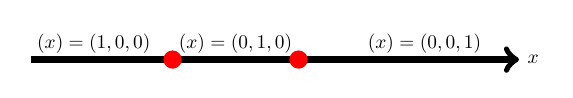
\begin{tikzpicture}[scale=0.2,every node/.style={scale=0.7}]
\draw[->,line width=0.08cm] (-5,0)--(26,0) node[right]{$\glssymbol{x}$};

\node [red,circle, fill] at (4,0) {};
\node [red,circle, fill] at (12,0) {};

\node at (-1,1) {$\q(x) = (1,0,0)$};
\node at (8,1) {$\q(x) = (0,1,0)$};
\node at (20,1) {$\q(x) = (0,0,1)$};
\end{tikzpicture}
\caption{\label{fig:disc_cont} Quantization (discretization) of a continuous feature.}
\end{minipage}

\vfill

\begin{minipage}{0.45\textwidth}
\centering
\begin{tikzpicture}[scale=0.2,every node/.style={scale=0.7}]
\tikzset{vertex/.style = {shape=circle,draw,scale=0.7,minimum size=1cm}}
\tikzset{edge/.style = {->,> = latex'}}

% Boules E^j
\node [vertex] (q1) at (3,2.5) {(1,0)};
\node [vertex] (q2) at (15,2.5) {(0,1)};

% Boules X^J
\node [vertex] (x1) at (-4,0) {0};
\node [vertex] (x2) at (1.8,0) {1};
\node [vertex] (x3) at (9.5,0) {2};
\node [vertex] (x4) at (17,0) {3};
\node [vertex] (x5) at (24,0) {4};

% Labels
\node at (-7,2.5) {$\q(x)=$};
\node at (-7,0.2) {$\glssymbol{x}=$};

% Flèches
\draw[edge,line width=0.03cm] (x1) to (q1);
\draw[edge,line width=0.03cm] (x3) to (q1);
\draw[edge,line width=0.03cm] (x4) to (q1);
\draw[edge,line width=0.03cm] (x2) to (q2);
\draw[edge,line width=0.03cm] (x5) to (q2);

\end{tikzpicture}
\caption{\label{fig:disc_disc} Quantization (factor levels merging) of categorical feature.}
\end{minipage}
\end{multicols}
\end{figure}


\paragraph{Notations for the quantization family}

In both continuous and categorical cases, keep in mind that $m_j$ is the dimension of $\q_j$. For notational convenience, the (global) order of the quantization $\q$ is set as 
\[|\q|=\sum_{j=1}^d m_j.\]
The space where quantizations $\q$ live (resp. $\q_j$) will be denoted by $\Q$ in the sequel (resp. $\Q_j$).

\subparagraph{Equivalence of quantizations} \label{par:equiv}

Let $\q^1$ and $\q^2$ in $\Q$ such that $\boldsymbol{f} \mathcal{R}_{\mathcal{T}_n} \boldsymbol{g} \equiv \forall i,j \; \q^1_j(x_i) = \q^2_j(x_i)$. See Figure~\ref{fig:equiv} for an example.

\subparagraph{Lemma} Relation $\mathcal{R}_{\mathcal{T}_n}$ defines an equivalence relation on $\Q$.

\begin{proof}
Relation $\mathcal{R}_{\mathcal{T}_n}$ is trivially reflexive and symmetric because of the reflexive and symmetric nature of the equality relation in $\glssymbol{R}$: $\forall i,j \; \q^1_j(x_i) = \q^1_j(x_i)$ and $\forall i,j \; \q^1(x_i) = \q^2(x_i)$. Similarly, let $\q^3 \in \Q$ such that $\q^1 \mathcal{R}_{\mathcal{T}_n} \q^3  \equiv \forall i,j \; \q^1_j(x_i) = \q^3_j(x_i)$. Again, we immediately get $\forall i,j \; \q^2_j(x_i) = \q^3_j(x_i)$, \textit{i.e.}\ $\q^2 \mathcal{R}_{\mathcal{T}_n} \q^3$ which proves the transitivity of $\mathcal{R}_{\mathcal{T}_n}$.
\end{proof}

 \begin{figure}[!ht]
     \centering
     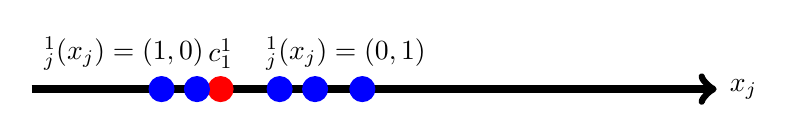
\begin{tikzpicture}[scale=0.3]
 \draw[->,line width=0.1cm] (-5,0)--(24,0) node[right]{$x_j$};

 \node [red,circle,fill] at (3,0) {};

 \node [blue,circle, fill] at (0.5,0) {};
 \node [blue,circle, fill] at (2,0) {};

 \node [blue,circle, fill] at (5.5,0) {};
 \node [blue,circle, fill] at (7,0) {};
 \node [blue,circle, fill] at (9,0) {};

 \node at (3,1.5) {$c^1_1$};

 \node at (-1.1,1.5) {$\q^1_j(x_j) = (1,0)$};
 \node at (8.3,1.5) {$\q^1_j(x_j) = (0,1)$};
 \end{tikzpicture}

 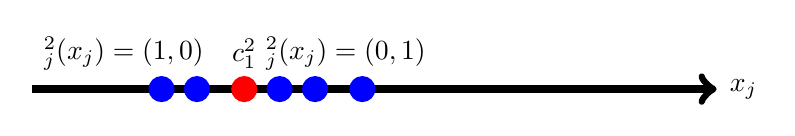
\begin{tikzpicture}[scale=0.3]
 \draw[->,line width=0.1cm] (-5,0)--(24,0) node[right]{$x_j$};

 \node [red,circle,fill] at (4,0) {};

 \node [blue,circle, fill] at (0.5,0) {};
 \node [blue,circle, fill] at (2,0) {};

 \node [blue,circle, fill] at (5.5,0) {};
 \node [blue,circle, fill] at (7,0) {};
 \node [blue,circle, fill] at (9,0) {};

 \node at (4,1.5) {$c^2_1$};

 \node at (-1.1,1.5) {$\q^2_j(x_j) = (1,0)$};
 \node at (8.3,1.5) {$\q^2_j(x_j) = (0,1)$};

 \end{tikzpicture}

     \caption{On the sample $\glssymbol{bbx}$ (blue points), the two discretization functions $\q^1$ and $\q^2$ (which respective unique cutpoint $c^1_1$ and $c^2_1$ are displayed in red) take the same value and are thus equivalent w.r.t. $\mathcal{R}_{\mathcal{T}_n}$.}
     \label{fig:equiv}
 \end{figure}


\subparagraph{Cardinality of the quantization family in the continuous case} ~\label{par:cardinality}

For a continuous feature $x_j$, let $\q_j \in \Q_j$ with $m_j$ intervals and cutpoints $\boldsymbol{c}_j$. Without any loss of generality, \textit{i.e.}\ up to a relabelling on individuals $i$, it can be assumed that there are $m_j+1$ observations $x_{1,j},\dots,x_{m_j+1,j}$ s.t.\ $x_{1,j} < c_{j,1} < x_{2,j} < \dots < c_{m_j-1,1} < x_{m_j+1,j}$. Indeed, if for example there exists $k < m_j - 1$ s.t.\ $c_{j,k} < \dots < c_{j,m_j-1}$ and $\max_{1 \leq i \leq n} x_{i,j} < c_{j,k}$, then discretization $\q^{\text{bis}}_j \in \Q_j$ with $k+1$ cutpoints $(-\infty,c_{j,1},\dots,c_{j,k-1},+\infty)$ is equivalent w.r.t.\ $\mathcal{R}_{\mathcal{T}_n}$ to $\q_j$: $\forall i, \; \q_j(x_{i,j}) = \q^{\text{bis}}_j(x_{i,j})$. A similar proof can be conducted with cutpoints below the minimum of $\glssymbol{bx}_j$ or with several cutpoints in-between consecutive values of the observations. Subsequently, there are $\binom{n-1}{m_j-1}$ ways to construct $\bm{c}_j$, \textit{i.e.}\ equivalence classes $[\q_j]$ for a fixed $m_j \leq n$. The number of intervals $m_j$ can range from $2$ (binarization) to $n$ (each $x_{i,j}$ is in its own interval, thus $\q_j(x_{i,j}) \neq \q_j(x_{i',j})$ for $i \neq i'$), so that the number of admissible discretization of $\glssymbol{bbx}_j$ is $|\Q_j| = \sum_{i=2}^{n}$ ${n-1}\choose{i-1}$. Note that $|\Q_j|$ depends on the number of observations $n$; I shall go back to this property in the following Section.


\subparagraph{Cardinality of the quantization family in the categorical case}

For a continuous feature $x_j$, let $\q_j \in \Q_j$ with $m_j$ groups. The number of re-arrangements of $l_j$ labelled elements into $m_j$ unlabelled groups is given by the Stirling number of the second kind $S(l_j,m_j) = \frac{1}{m_j!} \sum_{i=0}^{m_j} (-1)^{m_j-i} {m_j \choose i} i^{l_j}$. As $m_j$ is unknown and must be searched over the range $\{1,\dots,l_j\}$. Thus for categorical features, model space $\Q_j$ is also discrete; subsequently, $\Q = \prod_{j=1}^d \Q_j$ is discrete.







\paragraph{Literature review}

The current practice of quantization is prior to any predictive task, thus ignoring its consequences on the final predictive ability. It consists in optimizing a heuristic criterion, often totally unrelated (unsupervised methods) or at least explicitly (supervised methods) to prediction, and mostly univariate (each feature is quantized irrespective of other features' values). The cardinality of the quantization space $\Q$ can be calculated explicitely w.r.t.\ $d$, $(m_j)_1^d$ and, for categorical features, $l_j$. It is huge, so that a greedy approach is intractable and such heuristics are needed, as will be detailed in the next Section.
Many algorithms have thus been designed and a review of approximatively 200 discretization strategies, gathering both criteria and related algorithms, can be found in~\cite{ramirez2016data}, preceded by other enlightening review articles such as~\cite{dougherty1995supervised,liu2002discretization}. They classify discretization methods by distinguishing, among other criteria and as said previously, unsupervised and supervised methods ($\bm{y}$ is used to discretize $\bm{x}$), for which model-specific (assumptions on $p_{\glssymbol{bth}}$) or model-free approaches are distinguished, univariate and multivariate methods (features $X_{-\{j\}} = (X_{1},\ldots,X_{j-1},X_{j+1},\ldots,X_{d})$ may influence the quantization scheme) and other criteria as can be seen from Figure~\ref{fig:taxonomy} reproduced with permission. For factor levels grouping, I found no such taxonomy, but some discretization methods, \textit{e.g.}\ $\chi^2$ independence test-based methods can be naturally extended to this type of quantization, which is for example what the CHAID algorithm, proposed in~\cite{kass1980exploratory} and applied to each categorical feature, relies on. A simple idea is to use Group LASSO~\cite{meier2008group} which attempts to shrink to zero all coefficients of a categorical feature to avoid situations where a few levels enter the model, which is arguably less interpretable. Another idea would be to use Fused LASSO~\cite{tibshirani2005sparsity}, which seeks to shrink the pairwise absolute difference of selected coefficients, and apply it to all pairs of levels: the levels for which the difference would be shrunk to zero would be grouped. A combination of both approaches would allow both selection and grouping\footnote{See \url{https://stats.stackexchange.com/questions/60100/penalized-methods-for-categorical-data-combining-levels-in-a-factor}}.
For benchmarking purposes, and following results found in the taxonomy of~\cite{ramirez2016data}, I used the MDLP~\cite{fayyad1993multi} discretization method, described in-depth in Appendix~\ref{app1:mdlp}, which is a popular supervised univariate method, and I implemented an extension of ChiMerge to categorical features, performing pairwise $\chi^2$ independence tests rather than only pairs of contiguous intervals, which I called ChiCollapse and describe in-depth in Appendix~\ref{app1:chicollapse}. Note that various refinements of ChiMerge have been proposed in the literature, Chi2~\cite{liu1995chi2}, ConMerge~\cite{wang1998concurrent}, ModifiedChi2~\cite{tay2002modified}, and ExtendedChi2~\cite{su2005extended}, which seek to correct for multiple hypothesis testing~\cite{shaffer1995multiple} and automize the choice of the confidence parameter $\alpha$ in the $\chi^2$ tests, but adapting them to categorical features for benchmarking purposes would have been too time-consuming. A similar measure, called Zeta, has been proposed in place of $\chi^2$ in~\cite{ho1997zeta} and subsequent refinement~\cite{ho1998efficient}: it is the classification error achievable by using only two contiguous intervals; if it is low, the two intervals are dissimilar w.r.t.\ the prediction task, if not, they can be merged.

\begin{figure}[!ht]
\includegraphics[width=\textwidth]{figures/chapitre4/taxonomy.PNG}
\caption{Taxonomy of discretization methods.}
\label{fig:taxonomy}
\end{figure}



\subsection{Quantization embedded in a predictive process}

\paragraph{Logistic regression on quantized data}

Quantization is a widespread preprocessing step to perform a learning task consisting in predicting, say, a binary variable $\glssymbol{y}\in\{0,1\}$, from a quantized predictor  $\q(\glssymbol{bx})$, through, say, a parametric conditional distribution $p_{\glssymbol{bth}}(\glssymbol{y}|\q(\glssymbol{bx}))$ like logistic regression; the whole process can be visually represented as a dependence structure among $X$, its quantization $Q$ (which notation as a random variable will be made clearer in Section~\ref{sec:sem}) and the target $Y$ on Figure~\ref{fig:dep}. Considering quantized data instead of raw data has a double benefit. First, the quantization order $|\q|$ acts as a tuning parameter for controlling the model's flexibility and thus the bias/variance trade-off of the estimate of the parameter $\glssymbol{bth}$ (or of its predictive accuracy) for a given dataset. This claim becomes clearer with the example of logistic regression I focus on, as a still very popular model for many practitioners. It is classically described by
\begin{equation}
    \label{eq:reglogq}
\ln \left( \dfrac{p_{\glssymbol{bth}}(1|\q(\glssymbol{bx}))}{1 - p_{\glssymbol{bth}}(1|\q(\glssymbol{bx}))} \right) = \theta_0 + \sum_{j=1}^d \glssymbol{bth}_j' \cdot \q_j(\glssymbol{x}_j),
\end{equation}
where $\glssymbol{bth} = (\theta_{0},(\glssymbol{bth}_j)_1^d) \in \glssymbol{R}^{|\q|+1}$ and $\glssymbol{bth}_j = (\theta_{j}^{1},\dots,\theta_{j}^{m_j})$ with $\theta_{j}^{m_j} = 0$, $j=1 \ldots d$, for identifiability reasons.
Second, at the practitioner level, the previous tuning of $|\q|$ through each feature's quantization order $m_j$, especially when it is quite low, allows an easier interpretation of the most important predictor values involved in the predictive process. Denoting the dataset by $(\glssymbol{bbx},\glssymbol{bby})$, with $\glssymbol{bbx}=(\glssymbol{bx}_1,\ldots,\glssymbol{bx}_n)$ and $\glssymbol{bby}=(\glssymbol{y}_1,\ldots,\glssymbol{y}_n)$, the log-likelihood 
\begin{equation}
\label{eq:lq}
\ell_{\q}(\glssymbol{bth} ; (\glssymbol{bbx},\glssymbol{bby}))=\sum_{i=1}^n \ln p_{\glssymbol{bth}}(\glssymbol{y}_i|\q(\glssymbol{bx}_i))
\end{equation}
provides a Maximum Likelihood estimator $\hat{\glssymbol{bth}}_\q$ of $\glssymbol{bth}$ for a given quantization $\q$. For the rest of the chapter and consistently with the manuscript, the approach is exemplified with logistic regression as $p_{\glssymbol{bth}}$ but it can be applied to any other predictive model, as will be recalled in the concluding section.



\paragraph{Quantization as a model selection problem} \label{par:model_selec}

As dicussed in the previous section, and emphasized in the literature review, quantization is often a preprocessing step; however, quantization can be embedded directly in the predictive model. Continuouing our logistic example, a standard information criteria such as the BIC (see Section~\ref{subsubsec:choix_modele}) can be used to select the best quantization $\q$:
\begin{equation}
    \label{eq:BICq}
    \hat{\q}=\argmax_{\q \in \Q} \text{BIC}(\hat{\glssymbol{bth}}_\q)
\end{equation}
where $\nu_\q$ is traditionally the number of continuous parameters to be estimated in the $\glssymbol{bth}$-parameter space. Note however that an exhaustive search of $\hat{\q}\in\Q$ is an intractable task due to its highly combinatorial nature as was explicitly formulated in the previous Section. Anyway, the optimization~(\ref{eq:BICq}) requires a new specific strategy that I describe in the next section.

\paragraph{Remark on model selection consistency} \label{par:consistency}

In high-dimensional spaces and among models with a wildly varying number of parameters, classical model selection tools like BIC can have disappointing asymptotic properties, as emphasized in~\cite{chen2008extended}, where a modified BIC criterion, taking into account the number of models per parameter size, is proposed.
Moreover in essence, as is apparent from the $\hat{\glssymbol{bth}}_\q$ symbol, and supplemental to the \gls{lr} coefficients $\glssymbol{bth}$, the inherent parameters of $\q$, in the continuous case, which are the $c_{j,h}$ (see Equation~\eqref{eq:Cjhcont}) shall be accounted for in the penalization term $\nu_\q$: they are estimated indirectly in the subsequent Section.
In addition, in this setting, the BIC criterion relies on the Laplace approximation~\cite{lebarbier} which requires the likelihood to be twice differentiable in the parameters. However, as $\q$ consists in a collection of step functions of parameters $C_{j,h}$, this is not the case. For continuous features, since it is nevertheless almost everywhere differentiable, for the properties of the BIC criterion to hold, it suffices that there exists a neighbourhood $V_{j,h}$ around true parameters $c_{j,h}^\star$ where there is no observation: $\not\exists i, \: x_{i,j} \in V_{j,h}$.

\textcolor{red}{cas catégoriel : référence de Vincent (on ne peut pas compter les paramètres discrets)}

Lastly, for the asymptotic properties of BIC to hold in the case of nested models (which is not \textit{stricto sensu} the case here since for any global quantization order $|\q|$ there are a lot of possible univariate quantization orders $|\q_j|$), any multiplicative constant to the number of parameters is appropriate. Indeed, suppose two nested models $M_i$, $M_t$ have parameters $|\q|_i > |\q|_t$ respectively; then, we have:
\[ \text{BIC}_i - \text{BIC}_t \approx - \chi^2_{|\q|_i - |\q|_t} + C(|\q|_i - |\q|_t)\ln n, \]
where $C=1$ for the BIC criterion but could be replaced by any other $C \in \glssymbol{R}^+_\star$ since for $n \to + \infty$, $C(|\q|_i - |\q|_t)\ln n$ will dominate and reject the overly parametrized model $M_i$.

For all these reasons, the BIC criterion which penalizes only on the logistic regression parameters $\glssymbol{bth}$ is used in the remainder of this manuscript.

\section{The proposed neural network based quantization}
\label{sec:proposal}

\subsection{A relaxation of the optimization problem} \label{subsec:relaxation}

In this section, I propose to relax the constraints on $\q_j$ to simplify the search of $\hat{\q}$. Indeed, the derivatives of $\q_j$ are zero almost everywhere and consequently a gradient descent cannot be directly applied to find an optimal quantization.

\paragraph{Smooth approximation of the quantization mapping}

A classical approach is to replace the binary functions $q_{j,h}$ (see Equation (\ref{eq:qj}))  by smooth parametric ones  with a simplex condition, namely with $\ag_j=(\ag_{j,1},\ldots, \ag_{j,m_j})$:
%\begin{equation}
\begin{equation*}
    %\label{eq:qaj}
    {\q_{\ag_j}(\cdot)=\left(q_{\ag_{j,h}}(\cdot)\right)_{h=1}^{m_j} \text{ with } \sum_{h=1}^{m_j}q_{\ag_{j,h}}(\cdot)=1 \text{ and } 0 \leq q_{\ag_{j,h}}(\cdot) \leq 1,}
\end{equation*}
%\end{equation}
where functions $q_{\ag_{j,h}}(\cdot)$, properly defined hereafter for both continuous and categorical features, represent a fuzzy quantization in that, here, each level $h$ is weighted by $q_{\ag_{j,h}}(\cdot)$ instead of being selected once and for all as in (\ref{eq:qj}). The resulting fuzzy quantization for all components depends on the global parameter $\ag = (\ag_1, \ldots, \ag_d)$ and is denoted by $\q_{\ag}(\cdot)=\left(\q_{\ag_j}(\cdot)\right)_{j=1}^d$. 

%From a deterministic point of view, denoting by $\tilde{\Q}$ the space of $\q_{\ag}$, we have $\Q \subset \widetilde{\Q}$. From a statistical point of view, under standard regularity conditions and with a suitable estimation procedure (see later for the proposed estimation procedure), we have consistency of $(\q_{\hat{\ag}}, \hat{\glssymbol{bth}})$ towards $(\q,\glssymbol{bth})$. From an empirical point of view, we will see in Section~\ref{sec:experiments} and in particular in Figure~\ref{fig:MAP}, that this smooth approximation $\q_{\ag}$ converges towards ``hard'' quantizations\footnote{Up to a permutation on the labels $h=1 \ldots m_j$ to recover the ordering in $C_{j,h}$ (see Eq. (\ref{eq:Cjhcont})).} $\q$.



 {\bf For continuous features}, we set for $\ag_{j,h} = (\alpha^0_{j,h},\alpha^1_{j,h}) \in \glssymbol{R}^2$
\begin{equation} \label{eq:softmax}
q_{\ag_{j,h}}(\cdot) = \frac{\exp(\alpha^0_{j,h} + \alpha^1_{j,h}  \cdot)}{\sum_{g=1}^{m_j} \exp(\alpha^0_{j,g} + \alpha^1_{j,g}  \cdot)}
\end{equation}
where $\ag_{j,m_j}$ is set to $(0,0)$ for identifiability reasons.




{\bf For categorical features}, we set for $\ag_{j,h}=\left(\alpha_{j,h}(1),\ldots, \alpha_{j,h}(l_j)\right) \in \glssymbol{R}^{l_j}$
\[q_{\ag_{j,h}}(\cdot) = \frac{\exp\left(\alpha_{j,h}(\cdot)\right)}{\sum_{g=1}^{m_j} \exp\left(\alpha_{j,g}(\cdot)\right)}\]
where $l_j$ is the number of levels of the categorical feature $\glssymbol{x}_j$.

These approximations are justified by the following arguments. 

From a deterministic point of view, denoting by $\tilde{\Q}$ the space of $\q_{\ag}$, we have $\Q \subset \widetilde{\Q}$: First, the \textit{maximum a posteriori} step~(\ref{eq:ht}) produces contiguous intervals (\textit{i.e.}\ there exists $C_{j,h}$; $1 \leq j \leq d$, $1 \leq h \leq m_j$, s.t.\ ${\q}^{\text{MAP}}$ can be written as in~\ref{eq:qj}) \cite{same2011model}. Second, in the continuous case, the higher $\alpha_{j,h}^1$, the less smooth the transition from one quantization $h$ to its ``neighbor''\footnotemark[1] $h+1$, whereas $\dfrac{\alpha_{j,h}^0}{\alpha_{j,h}^1}$ controls the point in $\mathbb{R}$ where the transition occurs \cite{chamroukhi2009regression}. Concerning the categorical case, the rationale is even simpler as $q_{\lambda \alpha_{j,h}}(x_j) \to 1 \text{ if } h = \argmax_{h'} q_{\alpha_{j,h'}}(x_j), 0 \text{ otherwise}$ as $\lambda \to +\infty$~\cite{reverdy2016parameter}.

From a statistical point of view, 
%as $\ag$ needs to diverge to infinity for $\q_{{\ag}}$ to approximate $\q$, the maximum likelihood estimator of $\ag$ does not converge. However, 
under standard regularity conditions and with a suitable estimation procedure (see later for the proposed estimation procedure), the maximum likelihood framework ensures the consistency of $(\q_{\hat{\ag}}, \hat{\glssymbol{bth}})$ towards $(\q,\glssymbol{bth})$. This is further ensured by the \textit{maximum a posteriori} step~(\ref{eq:ht}).

However, and as is usual, the log-likelihood $\ell_{\q_{\ag}}(\glssymbol{bth},(\glssymbol{bbx},\glssymbol{bby}))$ cannot be directly maximized w.r.t.\ $(\ag,\glssymbol{bth})$, so that we need an iterative procedure. To this end, the next section introduces a neural network of particular architecture.

From an empirical point of view, we will see in Section~\ref{sec:experiments} and in particular in Figure~\ref{fig:MAP}, that the smooth approximation $\q_{\ag}$ converges towards ``hard'' quantizations\footnotemark[1] $\q$.


\footnotetext[1]{Up to a permutation on the labels $h=1 \ldots m_j$ to recover the ordering in $C_{j,h}$ (see Equation (\ref{eq:Cjhcont})).}


\paragraph{Parameter estimation}

With this new fuzzy quantization, the \gls{lr} for the predictive task is then expressed as
\begin{equation}
    \label{eq:reglogqa}
    \ln \left( \dfrac{p_{\glssymbol{bth}}(1|\q_{\ag} (\glssymbol{bx}))}{1 - p_{\glssymbol{bth}}(1|\q_{\ag} (\glssymbol{bx}))} \right) = \theta_0 + \sum_{j=1}^d {\glssymbol{bth}_j' \cdot \q_{\ag_{j}}(x_j)},
\end{equation}
where $\q$ has been replaced by $\q_{\ag}$ from Equation~(\ref{eq:reglogq}).
Note that as $\q_{\ag}$ is a sound approximation of $\q$ (see above), this \gls{lr} in $\q_{\ag}$ is consequently a good approximation of the \gls{lr} in $\q$ from Equation~(\ref{eq:reglogq}). The relevant log-likelihood is here 
\begin{equation}
    \label{eq:lqa}
    \ell_{\q_{\ag}}(\glssymbol{bth} ; (\glssymbol{bbx},\glssymbol{bby}))=\sum_{i=1}^n \ln p_{\glssymbol{bth}}(y_i|\q_{\bm{\alpha}}(\bm{x}_i))
\end{equation}
and can be used as a tractable substitute for (\ref{eq:lq}) to solve the original optimization problem (\ref{eq:BICq}), where now both $\ag$ and $\glssymbol{bth}$ have to be estimated, which is discussed in the next section. We wish to maximize the log-likelihood (\ref{eq:reglogqa}) which would yield parameters $(\hat{\ag},\hat{\glssymbol{bth}})$; these are consistent if the model is well-specified (\textit{i.e.}\ there is a ``true'' quantization under classical regularity conditions). To ``push'' $\widetilde{\Q}$ further into $\Q$, $\hat{\q}$ is deduced from a \textit{maximum a posteriori} procedure applied to $\q_{\hat{\ag}}$:
\begin{equation}
    \label{eq:ht}
    \hat{q}_{j,h}(x_j) = 1 \text{ if } h = \argmax_{1 \leq h' \leq m_j} q_{\hat{\ag}_{j,h'}}, 0 \text{ otherwise.}
\end{equation}
If there are several levels $h$ that satisfy (\ref{eq:ht}), we simply take the level that corresponds to smaller values of $x_j$ to be in accordance with the definition of $C_{j,h}$ in Equation~(\ref{eq:Cjhcont}). This {\it maximum a posteriori} principle will be exemplified in Figure~\ref{fig:MAP} on simulated data.


\subsection{A neural network-based estimation strategy} \label{sec:estim}

\paragraph{Neural network architecture}

To estimate parameters $\ag$ and $\glssymbol{bth}$ in the model (\ref{eq:reglogqa}), a particular neural network architecture can be used. The most obvious part is the output layer that must produce $p_{\glssymbol{bth}}(1|\q_{\ag}(\glssymbol{bx}))$ which is equivalent to a densely connected layer with a sigmoid activation $\sigma (\cdot)$.

For a continuous feature $\glssymbol{x}_j$ of $\glssymbol{bx}$, the combined use of $m_j$ neurons including affine transformations and softmax activation obviously yields $\q_{\ag_{j}}(x_j)$. Similarly, an input categorical feature $\glssymbol{x}_j$ with $l_j$ levels is equivalent to $l_j$ binary input neurons (presence or absence of the factor level). These $l_j$ neurons are densely connected to $m_j$ neurons without any bias term and a softmax activation. The softmax outputs are next aggregated via the summation in model (\ref{eq:reglogqa}), say $\Sigma_{\glssymbol{bth}}$ for short, and then the sigmoid function $\sigma$ gives the final output. All in all, the proposed model is straightforward to optimize with a simple neural network, as shown in Figure~\ref{fig:nn}.


\def\layersep{2.5cm}

\begin{figure}[!ht]
\centering
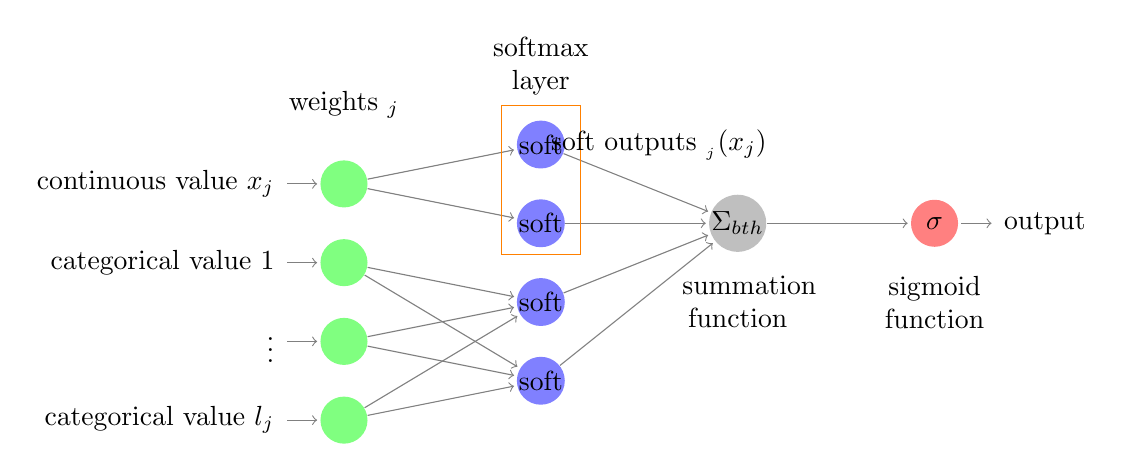
\begin{tikzpicture}[shorten >=1pt,->,draw=black!50, node distance=\layersep]
    \tikzstyle{every pin edge}=[<-,shorten <=1pt]
    \tikzstyle{neuron}=[circle,fill=black!25,minimum size=17pt,inner sep=0pt]
    \tikzstyle{input neuron}=[neuron, fill=green!50];
    \tikzstyle{output neuron}=[neuron, fill=red!50];
    \tikzstyle{hidden neuron}=[neuron, fill=blue!50];
    \tikzstyle{annot} = [text width=4em, text centered]
    \tikzstyle{annotrectangle} = [text width=8em, text centered]


        \node[input neuron, pin=left:continuous value $x_j$] (I-1) at (0,-1) {};
        
        \node[input neuron, pin=left:categorical value $1$] (I-2) at (0,-2) {};
        \node[input neuron, pin=left:$\vdots$] (I-3) at (0,-3) {};
        \node[input neuron, pin=left:categorical value $l_j$] (I-4) at (0,-4) {};

    % Draw the hidden layer nodes
    \foreach \name / \y in {1,...,2}
        \path[yshift=0.5cm]
            node[hidden neuron] (H-\name) at (\layersep,-\y cm) {soft};

    \foreach \name / \y in {3,...,4}
        \path[yshift=0.5cm]
            node[hidden neuron] (H-\name) at (\layersep,-\y cm) {soft};
            
    % Draw the sum layer node 
    
    \node[neuron, right of=H-2] (S) {$\Sigma_{\glssymbol{bth}}$};

    % Draw the output layer node
    
    \node[output neuron,pin={[pin edge={->}]right:output}, right of=S] (O) {$\sigma$};
    
    %\node[output neuron,pin={[pin edge={->}]right:Output}, right of=H-2] (O) {$\sigma(\cdot)$};
    
    

    % Connect every node in the input layer with every node in the
    % hidden layer.
%    \foreach \source in {1,...,4}
        \foreach \dest in {1,2}
            \path (I-1) edge (H-\dest);

        \foreach \dest in {3,4}
            \path (I-2) edge (H-\dest);
        \foreach \dest in {3,4}
            \path (I-3) edge (H-\dest);
        \foreach \dest in {3,4}
            \path (I-4) edge (H-\dest);

        % \foreach \dest in {5,6}
        %     \path (I-3) edge (H-\dest);

    % Connect every node in the hidden layer with the output layer
    \foreach \source in {1,...,4}
        \path (H-\source) edge (S);
        
    % connect Sigma with sigma
    \path (S) edge (O);

    % Annotate the layers
    \node[annot,above of=H-1, node distance=1cm] (hl) {softmax layer};
    \node[annot,above of=I-1,node distance=1cm] {weights $\ag_j$};
    %\node[annot,right of=hl] (s) {};
    \node[annot, below of=O, node distance=1cm] (s) {sigmoid function};
    \node[annot, below of=S,node distance=1cm] {summation function};
    
    \draw [orange] (2,0) rectangle (3,-1.9);
    % \draw [red] (2,-2) rectangle (3,-4);
    
    \node[annotrectangle,right of=H-1, node distance=1.5cm] {soft outputs $\q_{\ag_j}(x_j)$}; 

\end{tikzpicture}
\caption{Proposed shallow architecture to maximize (\ref{eq:lqa}).}
\label{fig:nn}
\end{figure}


\paragraph{Stochastic gradient descent as a quantization provider}

By relying on stochastic gradient ascent, the smoothed likelihood (\ref{eq:lqa}) can be maximized over $\left(\ag, \glssymbol{bth} \right)$. Due to its convergence properties~\cite{bottou2010large}, the results should be close to the maximizers of the original likelihood (\ref{eq:lq}) if the model is well-specified, when there is a true underlying quantization. However, in the mis-specified model case, there is no such guarantee. Therefore, to be more conservative, we evaluate at each training epoch $(t)$ the quantization ${\q}^{\text{MAP}(t)}$ resulting from the \textit{maximum a posteriori} procedure explicited in Equation~(\ref{eq:ht}), then classically estimate the logistic regression parameter \textit{via} maximum likelihood, as done in Equation~(\ref{eq:lq}):
\[\hat{\glssymbol{bth}}^{(s)} = \argmax_{\glssymbol{bth}} \ell_{\hat{q}^{(s)}}(\glssymbol{bth}; (\glssymbol{bbx},\glssymbol{bby}))\]
and the resulting $\mbox{BIC}(\hat{\glssymbol{bth}}^{(s)})$ as in (\ref{eq:BICq}). If $T$ is a given maximum number of iterations of the stochastic gradient descent algorithm, the quantization retained at the end is then determined by the optimal epoch
\begin{equation} \label{eq:opt_epoch}
s_\star=\argmin_{t\in \{1,\ldots, T\}} \mbox{BIC}(\hat{\glssymbol{bth}}^{(s)}).
\end{equation}

Lots of optimization algorithms for neural networks have been proposed, which all come with their hyperparameters. As, in the general case, $\ell_{\q_{\ag}}(\glssymbol{bth} ; (\glssymbol{bbx},\glssymbol{bby}))$ of Equation~\eqref{eq:lqa} is not guaranteed to be convex, there might be several local maxima, such that all these optimization methods might diverge, converge to a different maximum, or at least converge in very different numbers of epochs, as can be examplified in Animation~\ref{fig:anim_sgd}\footnote{Reproduced from \url{https://github.com/wassname/viz_torch_optim}}. I chose the RMSProp method, which showed good results and is one of the standard methods.

%\begin{figure}[!ht]
%\begin{animateinline}[poster=first, controls=all, palindrome, autopause, autoresume, width=\textwidth]{3}
%\multiframe{300}{i=1+1}{\includegraphics{figures/chapitre4/optimization_methods/viz-\i.png}}%
%\end{animateinline}
%\caption{\label{fig:anim_sgd} Animation of several optimization methods (the $\star$ denotes the global maximum).}
%\end{figure}

 
\paragraph{Choosing an appropriate number of levels}

Concerning now the number of intervals or factor levels $\boldsymbol{m} = (m_j)_1^d$, they have also to be estimated since in practice they are unknown. Looping over all candidates $\boldsymbol{m}$ is intractable. But in practice, by relying on the \textit{maximum a posteriori} procedure developed in Equation~(\ref{eq:ht}), a lot of unseen factor levels might be dropped, \textit{e.g.}\ if $q_{\ag_{j,h}}(x_{i,j}) \ll 1$ for all training observations $\glssymbol{xij}$, the level $h$ ``vanishes'', \textit{i.e.}\ $\hat{q}_{j,h} = 0$. In practice, I recommend to start with a user-chosen $\bm{m}=\boldsymbol{m}_{\max}$ and we will see in the experiments of Section~\ref{sec:experiments} that the proposed approach is able to explore small values of $\boldsymbol{m}$ and to select a value $\hat{\boldsymbol{m}}$ drastically smaller than $\boldsymbol{m}_{\max}$. This phenomenon, which reduces the computational burden of the quantization task, is also illustrated in Section~\ref{sec:experiments}.

The full algorithm is described in Appendix~\ref{app1:glmdiscNN}.


\section{An \gls{sem} approach} \label{sec:sem}
 
 
In what follows, the quantization $\q(\glssymbol{bx})$ is seen as a latent feature denoted by $\bm{\mathfrak{Q}}$. The same notations can be introduced for this new feature:  $\bqk$ is an observation of $\bm{\mathfrak{Q}}$, $\bqk_j$ will designate the $j^{\text{th}}$ vectorial component of $\bqk$, $\bbqk$ will designate the $n$-sample where $\bbqk_i$ is its $i^{\text{th}}$ row
%, corresponding to an observation
, and so on. In the following Section, I translate earlier assumptions in probabilitics terms. In the subsequent Section, I make good use of these assumptions to provide a continuous relaxation of the quantization problem, as was empirically argumented in Section~\ref{subsec:relaxation}. This relaxation is equivalent to the one proposed in Section~\ref{sec:proposal}, although its use differs drastically, as will be emphasized in Section~\ref{subsec:stoch}.

\subsection{Probabilistic assumptions regarding the quantization latent feature}

Firstly, only the well-specified model case is considered, which translates, with this new latent feature, as a probabilistic assumption:
\begin{equation} \label{hyp:true}
\exists \glssymbol{bth}^\star, \bqk^\star \text{s.t.\ } Y \sim p_{\glssymbol{bth}^\star}(\cdot | \bqk^\star)
\end{equation}
Secondly, the result of the quantization is assumed to be ``self-contained'' w.r.t.\ predictive information in $\glssymbol{bx}$, \textit{i.e.}\ it is assumed all available information about $y$ in $\glssymbol{bx}$ has been ``squeezed'' by quantizing the data:
\begin{equation} \label{hyp:squeeze}
\forall \glssymbol{bx},y,\: p(y|\glssymbol{bx},\bqk) = p(y|\bqk)
\end{equation}
Thirdly, the component-wise nature of the quantization can be stated as:
\begin{equation} \label{hyp:component}
\forall \glssymbol{bx},\bqk,\: p(\bqk|\glssymbol{bx}) = \prod_{j=1}^d p(\bqk_j | x_j)
\end{equation}



\subsection{Continuous relaxation of the quantization as seen as fuzzy assignment} \label{subsec:fuzzy}

If we consider the deterministic discretization scheme defined in Section~\ref{sec:model_selection}, we have, analogous to Equation~\eqref{eq:qj}:
$$
p(\bqk_j | x_j) = 1 \text{ if } x_j \in C_{j,h} \text{ and } \qk_{j,h} = 1, 1 \leq h \leq m_j,
$$
which is a step function. Rewriting $p(y| \glssymbol{bx})$ by integrating over these new latent features,
% and using hypotheses~\ref{hyp:true}, \ref{hyp:squeeze} and \ref{hyp:component} respectively, 
we get:
\begin{align*}
p(y | \glssymbol{bx}) & = p_{\glssymbol{bth}^\star}(y | \bqk^\star) & \text{ (using \eqref{hyp:true}) } \\
& = \sum_{\bqk \in \Q} p(y, \bqk | \glssymbol{bx}) \\
& = \sum_{\bqk \in \Q} p(y | \bqk, \glssymbol{bx}) p(\bqk | \glssymbol{bx}) \\
& = \sum_{\bqk \in \Q} p(y | \bqk) p(\bqk | \glssymbol{bx}) & \text{ (using \eqref{hyp:squeeze}) } \\
& = \sum_{\bqk \in \Q} p(y | \bqk) \prod_{j=1}^d p(\bqk_j | x_j) & \text{ (using \eqref{hyp:component}) }
\end{align*}
The well-specified model hypothesis~\eqref{hyp:true} yields for all $x_j$, $p(\bqk_j^\star | x_j) = 1$. Conversely, for $\bqk \in \Q$ such that $\bqk \cancel{\mathcal{R}_{\mathcal{T}_n}} \bqk^\star$, there exists a feature $j$ and an observation $x_{i,j}$ such that $p(\bqk_j | x_j) = 0$. Consequently, the above sum, over all training observations in $\mathcal{T}_n$, reduces to:
\begin{align*}
p(\glssymbol{bby} | \glssymbol{bbx}) & = \prod_{i=1}^n p(y_i | \glssymbol{bx}_i) \\
 & = \sum_{\bqk \in \Q} \prod_{i=1}^n p(y_i | \bqk_i) \prod_{j=1}^d p(\bqk_{i,j} | x_{i,j}) \\
 & = \prod_{i=1}^n p(y_i | \bqk_i^\star) \prod_{j=1}^d p(\bqk_{i,j}^\star | x_{i,j})
\end{align*}
Thus, we have :
\[ \bqk^\star = \argmax_{\bqk \in \Q} \prod_{i=1}^n p(y_i | \bqk_i ) \prod_{j=1}^d p(\bqk_{i,j} | x_{i,j}). \]
This new formulation of the best quantization is still untractable since it requires to evaluate all quantizations in $\Q$, although all terms except $\bqk^\star$ contribute to $0$ in the above $\argmax$. In the misspecfied model-case however, there is no such guarantee but it can still be claimed that the best candidate $\bqk^\star$ in terms of criterion~\eqref{eq:BICq} dominates the sum.

Our goal in the next Section is to generate good candidates $\bbqk$ as in Section~\ref{sec:estim}. Among other things detailed later on, models for $p(\glssymbol{bby} | \bqk)$ and $p(\bqk_j | x_j)$ shall be proposed. If the resulting MCMC is efficient, $\q_\star$ will be the mode of the empirical distribution of generated candidates, which, as in Section~\ref{sec:proposal} with the neural network approach, can be selected with the BIC criterion~\eqref{eq:BICq}. Using \eqref{hyp:true}, it seems most natural to use a \gls{lr} for $p( y | \bqk_j)$. Following Section~\ref{sec:proposal} and as was empirically argumented in Section~\ref{subsec:relaxation}, $p(\bqk_j | x_j)$ will be parametrized by $\ag_j$. 

{\bf For a continuous feature}, we resort to a polytomous logistic regression, similar to the softmax function of Equation~\eqref{eq:softmax} without the over-parametrization (one level per feature $j$, say $m_j$, is considered reference):
\[ p_{\ag_{j,h}}(\bqk_j | x_j) = \begin{cases} \frac{1}{\sum_{h'=1}^{m_j-1} \exp(\alpha_{j,h'}^0 + \alpha_{j,h'}^1 x_j)} \text{ if } h = m_j, \\ \frac{\alpha_{j,h}^0 + \alpha_{j,h}^1 x_j}{\sum_{h'=1}^{m_j-1} \exp(\alpha_{j,h'}^0 + \alpha_{j,h'}^1 x_j)} \text{ otherwise.} \end{cases} \]
{\bf For categorical features}, simple contingency tables are employed:
\[ p_{\ag_{j,h}^o}(\bqk_j | x_j) = \frac{|\bbqk_{j,h}|}{|\{x_j=o\}|} \text{ for } 1 \leq o \leq l_j \]
Similarly, $p_{\ag_j}(\bqk_j | x_j)$ are no more step functions but smooth functions as in Figure~\ref{fig:MAP}.

\paragraph{Remark on polytomous logistic regressions}

Since the resulting latent categorical feature can be interpreted as an ordered categorical features (the \textit{maximum a posterior} operation yields contiguous intervals as argued in Section~\ref{subsec:relaxation}), ordinal ``parallel'' logistic regression~\cite{o2006logistic} could be used (provided levels $h$ are reordered). This particular model is of the form:
\[ \ln \frac{p(\bqk_{j,h+1} = 1 | x_j)}{p(\bqk_{j,h} = 1 | x_j)} = \alpha_{j,h,0} + \alpha_{j,h} x_j, 1 \leq h < m_j, \]
which restricts the number of parameters since all levels share the same slope. Its advantages lie in the fact that it might lead to sharper door functions quicker, and that it has fewer parameters to estimate, thus reducing \textit{de facto} the estimation variance of each ``soft'' quantization. However, it makes it harder for levels to ``vanish'' which would require to iterate over the number of levels per feature $m_j$ which we wanted to avoid. In practice, it yielded similar results to polytomous logistic regression such that they remain a parameter of the \textsf{R} package \textit{glmdisc} (see Appendix~\ref{app2}).

\subsection{Stochastic search of the best quantization} \label{subsec:stoch}

We parametrized $p(y|\glssymbol{bx})$ as:
\begin{equation}
p(y | \glssymbol{bx}, \glssymbol{bth}, \ag) = \sum_{\bqk \in \Q} p_{\glssymbol{bth}}(y | \bqk) \prod_{j=1}^d p_{\ag_j}(\bqk_j | \glssymbol{bbx}_j)
\end{equation}
A straightforward way to maximize the likelihood of $p(y | \glssymbol{bx}, \glssymbol{bth}, \ag)$ in $(\glssymbol{bth}, \ag)$ (not to be mistaken with~\eqref{eq:lqa}), as was done in Section~\ref{sec:proposal}, to deduce $\q^\star$ from $\ag$ \textit{via} the $\argmax$ operation (see Section~\ref{subsec:relaxation} and Equation~\eqref{eq:ht}), is to use an \gls{em} algorithm~\cite{dempster1977maximum}.

However, maximizing this likelihood directly is untractable as the Expectation step requires to sum over $\bqk \in \Q$. Classically, the \gls{em} can be replaced by an MCMC method called \acrlong{sem}~\cite{celeux1985sem}: the expectation (the sum over $\bqk \in \Q$) is approximated by the empirical distribution of draws $\bqk^{(1)}, \dots, \bqk^{(\max\_{\text{iter}})}$ from $p_{\glssymbol{bth}}(y | \cdot) \prod_{j=1}^d p_{\ag_j}(\cdot | x_j)$.

\subsubsection{\gls{sem} as a quantization provider}

As the parameters $\ag$ of $\q_{\ag}$ were initialized randomly in the neural network approach, the latent features observations $\bbqk^{(0)}$ are initialized randomly. At step $s$, the \gls{sem} algorithm allows us to compute the MLE of $\glssymbol{bth}$ (resp. $\ag$) as $\hat{\glssymbol{bth}}^{(s)}$ (resp. $\hat{\ag}^{(s)}$) given $\bbqk^{(s)}$ by maximizing the following likelihoods:
\begin{alignat}{2}
\hat{\glssymbol{bth}}^{(s)} & = \argmax_{\glssymbol{bth}} \ell(\glssymbol{bth}; \bbqk^{(s)}, \glssymbol{bby}) && = \argmax_{\glssymbol{bth}} \sum_{i=1}^n \ln p_{\glssymbol{bth}}(y_i | \bqk^{(s)}_i), \nonumber \\
\hat{\ag_j}^{(s)} & = \argmax_{\ag_j} \ell(\ag_j; \glssymbol{bbx}_j, \bbqk^{(s)}_j) && = \argmax_{\ag_j} \sum_{i=1}^n \ln p_{\ag_j}(\bqk^{(s)}_{i,j} | x_{i,j}) \text{ for } 1 \leq j \leq d. \label{eq:mle_ag}
\end{alignat}

As the \gls{lr} $p_{\glssymbol{bth}}(y | \bqk)$ is multivariate, it is hard to sample simultaneously all latent features. We have to resort to the Gibbs-sampler~\cite{casella1992explaining}: $\bqk_j$ is sampled while holding latent features $\bqk_{-\{j\}}$ fixed:
\begin{equation} \label{eq:q_draw}
\bqk_j^{(s+1)} \sim p_{\hat{\glssymbol{bth}}^{(s)}}(y | \bqk_{-\{j\}}^{(s)}, \cdot) p_{\hat{\ag}^{(s)}}(\cdot | x_j)
\end{equation}
This process is repeated for all features $1 \leq j \leq d$.

%This MCMC provides parameters $\hat{\ag}^{(1)}, \dots, \hat{\ag}^{(\max\_{\text{iter}})}$ which can be used to produce $\hat{\q}^{(1)}, \dots, \hat{\q}^{(\max\_{\text{iter}})}$ following the \textit{maximum a posteriori} scheme from Equation~\eqref{eq:ht}. The best proposed quantization $\q^\star$ is thus chosen among them \textit{via} the BIC criterion as in Equation~\eqref{eq:opt_epoch}.


\subsubsection{Validity of the approach}

The pseudo-completed sample $(\glssymbol{bbx}, \bbqk^{(s)}, \glssymbol{bby})$ allows to compute $(\hat{\glssymbol{bth}}^{(s)},\hat{\ag}^{(s)})$ which do not converge to the MLE of $p(\glssymbol{bby} | \glssymbol{bbx}, \glssymbol{bth}, \ag)$, for the simple reason that, being random in essence, it does not converge pointwise. From its authors, the \gls{sem} is however expected to be directed by the \gls{em} dynamics~\cite{celeux_sem} and as any MCMC approach, its empirical distribution converges to the target distribution $p(\glssymbol{bby} | \glssymbol{bbx}, \glssymbol{bth}, \ag)$ provided such a distribution exists and is unique. This existence is guaranteed by remarking that for all features $j$, $ p(\bqk_j | x_j, \bqk^{(s)}_{-\{j\}} y, \glssymbol{bth}, \ag) \propto p_{\glssymbol{bth}}(y | \bqk^{(s)}_{-\{j\}}, \bqk_j) p_{\ag_j}(\bqk_j | x_j) > 0 $ by definition of the \gls{lr} and polytomous logistic regressions or the contingency tables respectively. The uniqueness is not guaranteed since levels can disappear and there is an absorbing state (the empty model): this point is detailed in the next Section.

In its original purpose~\cite{celeux_sem}, the \gls{sem} was employed either to find good starting points for the \gls{em} (\textit{e.g.}\ to avoid local maxima) or to propose an estimator of the MLE of the target distribution as the mean or the mode of the resulting empirical distribution, eventually after a burn-in phase. As, in our setting, we are not directly interested in the MLE but only to the best quantization in the sense of Equation~\eqref{eq:BICq}, we compute $\hat{\q}^{(1)}, \dots, \hat{\q}^{(\max\_{\text{iter}})}$ following the \textit{maximum a posteriori} scheme from Equation~\eqref{eq:ht}. The best proposed quantization $\q^\star$ is thus chosen among them \textit{via} the BIC criterion as in Equation~\eqref{eq:opt_epoch}.

\subsubsection{Choosing an appropriate number of levels}

Contrary to the neural network approach developed in Section~\ref{sec:proposal}, the \gls{sem} algorithm alternates between drawing $\bbqk^{(s)}$ and fitting $\hat{\glssymbol{bth}}^{(s)}$ and $\hat{\ag}^{(s)}$  at each step $s$. Therefore, additionally to the phenomenon of ``vanishing'' levels caused by the \textit{maximum a posteriori} procedure similar to the neural network approach, if a level $h$ of $\bqk$ is not drawn, following Equation~\eqref{eq:q_draw}, at step $s$, then at step $s+1$ when adjusting parameters $\ag_j$ by maximum likelihood from Equation~\eqref{eq:mle_ag}, this level will have disappeared and cannot be drawn again. A Reversible-Jump MCMC approach would be needed~\cite{green1995reversible} to ``resuscitate'' these levels, which is not needed in the neural network approach because its architecture is fixed in advance. As a consequence, with a design matrix of fixed size $n$, there is a non-zero probability that for any given feature, any of its levels collapses at each step such that $m_j^{(s+1)} \leftarrow m_j^{(s)} - 1$.

The MCMC has thus an absorbing state for which all features are quantized into one level (the empty model with no features) which is reached in a finite number of steps (although very high if $n$ is sufficiently large as is the case with \textit{Credit Scoring} data). The \gls{sem} algorithm is an effective way to start from a high number of levels per feature $\bm{m}_{\max}$ and explore smaller values.

The full algorithm is described in Appendix~\ref{app1:glmdiscSEM}.

\section{Numerical experiments} \label{sec:experiments}

This section is divided into three complementary parts to assess the validity of our proposal, that I call hereafter \textit{glmdisc}-NN and \textit{glmdisc}-SEM, designating respectively the approaches developed in Sections~\ref{sec:proposal} and~\ref{sec:sem}. First, simulated data are used to evaluate its ability to recover the true data generating mechanism. Second, the predictive quality of the new learned representation approach is illustrated on several classical benchmark datasets from the UCI library. Third, I use it on \textit{Credit Scoring} datasets provided by Credit Agricole Consumer Finance, a major European company in the consumer credit market. The code of all experiments, excluding the confidential real data, can be retrieved following the guidelines in Appendix~\ref{app2}.


\subsection{Simulated data: empirical consistency and robustness}

I focus here on discretization of continuous features (similar experiments could be conducted on categorical ones). Two continuous features $x_1$ and $x_2$ are sampled from the uniform distribution on $[0,1]$ and discretized as exemplified on Figure~\ref{fig:exp_sim} by using
\[\q_1(\cdot)=\q_2(\cdot) = (\mathds{1}_{]-\infty,1/3]}(\cdot),\mathds{1}_{]1/3,2/3]}(\cdot),\mathds{1}_{]2/3,\infty[}(\cdot)).\]
Here, following (\ref{eq:Cjhcont}), we have $d=2$ and $m_1=m_2=3$ and the cutpoints are $c_{j,1}=1/3$ and $c_{j,2}=2/3$ for $j=1,2$. Setting $\glssymbol{bth}=(0,-2,2,0,-2,2,0)$, the target feature $y$ is then sampled from $p_{\glssymbol{bth}}(\cdot | \q(\glssymbol{bbx}))$ via the logistic model (\ref{eq:reglogq}).

\begin{figure}[!ht]
\centering
\begin{tikzpicture}
      \draw[->] (-1,0) -- (9,0) node[right] {$x$};
      \draw[->] (0,-1) -- (0,3) node[above] {$p(x)$};
      \draw[scale=1,domain=0.5:7,smooth,variable=\y,red,thick]  plot ({\y},2.5);
      \draw[scale=1,domain=-1:0.5,smooth,variable=\y,red,thick]  plot ({\y},0);
      \draw[scale=1,domain=7:8.5,smooth,variable=\y,red,thick]  plot ({\y},0);
      \draw[scale=1,domain=0:2.5,smooth,variable=\x,red]  plot (0.5,{\x});
      \draw[scale=1,domain=0:2.5,smooth,variable=\x,red]  plot (7,{\x});
      
      \draw[scale=1,domain=-0.2:2.8,smooth,variable=\x,blue]  plot (2.67,{\x});
      \draw[scale=1,domain=-0.2:2.8,smooth,variable=\x,blue]  plot (4.83,{\x});

		\node[scale=0.7] (q1) at  (1.2,2.7) {\small $\q(x)=(1,0,0)$};
		\node[scale=0.7] (q2) at  (3.5,2.7) {\small $\q(x)=(0,1,0)$};
		\node[scale=0.7] (q3) at  (6,2.7) {\small $\q(x)=(0,0,1)$};

		\node[scale=0.7] (x1) at  (0.5,-0.5) {$0$};
		\node[scale=0.7] (x2) at  (2.67,-0.5) {$c_1=1/3$};
		\node[scale=0.7] (x3) at  (4.83,-0.5) {$c_2=2/3$};
		\node[scale=0.7] (x4) at  (7,-0.5) {$1$};

\end{tikzpicture}
\caption{\label{fig:exp_sim} Pdf of the simulated continuous data $x$ and the true quantization $\q$.}
\end{figure}


From the \textit{glmdisc} algorithm, I studied three cases:
\begin{enumerate}[(a)]
    \item First, the quality of the cutoff estimator $\hat{c}_{j,2}$ of $c_{j,2} = 2/3$ is assessed when the starting maximum number of intervals per discretized continuous feature is set to its true value $m_1=m_2= 3$;
    \item Second, I estimated the number of intervals $\hat{m}_1$ of $m_1=3$ when the starting maximum number of intervals per discretized continuous feature is set to $m_{\text{max}} = 10$; 
    \item Last, I added a third feature $x_3$ also drawn uniformly on $[0,1]$ but uncorrelated to $y$ and estimated the number $\hat{m}_3$ of discretization intervals selected for $x_3$. The reason is that a non-predictive feature which is discretized or grouped into a single value is \textit{de facto} excluded from the model, and this is a positive side effect.
\end{enumerate}
From a statistical point of view, experiment (a) assesses the empirical consistency of the estimation of $C_{j,h}$, whereas experiments (b) and (c) focus on the consistency of the estimation of $m_j$. The results are summarized in Table~\ref{tab:estim_precision} where 95\% confidence intervals (CI~\cite{sun2014fast}) are given, with a varying sample size. Note in particular that the slight underestimation in (b) is a classical consequence of the BIC criterion on small samples. 

\begin{table}[ht]
    \centering
    \caption{For \textit{glmdisc}-NN and \textit{glmdisc}-SEM and different sample sizes $n$, (A) CI of $\hat{c}_{j,2}$ for $c_{j,2} = 2/3$. (B) Bar plot of $\hat{m} = 2, 3, 4$ (resp.) for $m_1=3$. (C) Bar plot of $\hat{m}_3 = 1, 2, 3$ (resp.) for $m_3=1$.}
    \label{tab:estim_precision}
\begin{tabular}{lllllll}
Algorithm & $n$ & (a) $\hat{c}_{j,2}$ & (b) & $\hat{m}_1$ & (c) & $\hat{m}_3$ \\
\hline
\textit{glmdisc}-NN & $1{,}000$ & $[0.656,0.666]$ & \myobar{9}{90}{1} & \mybar{60}{32}{8} \\
\textit{glmdisc}-SEM & $1{,}000$ & $[0.656,0.666]$ & \myobar{2}{53}{44} & \mybar{34}{56}{10} \\
\textit{glmdisc}-NN & $10{,}000$ & $[0.666,0.666]$ & \myobar{0}{100}{0} & \mybar{88}{12}{0} \\
\textit{glmdisc}-SEM & $10{,}000$ & $[0.666,0.666]$ & \myobar{0}{100}{0} & \mybar{30}{48}{22}
\end{tabular}
\end{table}

To complement these experiments on simulated data following a well-specified model, a similar study can be done for categorical features: 10 levels are drawn uniformly and 3 groups of levels, which share the same log-odd ratio, are created. The same phenomenon as in Table~\ref{tab:estim_precision} is witnessed: the empirical distribution of the estimated number of groups of levels is peaked at its true value of 3.

Finally, it was argued in Section~\ref{sec:model_selection} that by considering all features when quantizing the data, .

\textcolor{red}{commenter le tableau et donner le mécanisme de génération de données}

\begin{table}[ht]
    \centering
    \caption{Gini of the resulting misspecified \gls{lr} from quantized data using ChiMerge, MDLP and \textit{glmdisc}-SEM: the multivariate approach is able to capture information about the correlation structure.}
    \label{tab:sim_false}
\begin{tabular}{llll}
 & ChiMerge & MDLP & \textit{glmdisc}-SEM \\
\hline
Performance & 50.1 (1.6) & 77.1 (0.9) & \textbf{80.6} (0.6)
\end{tabular}
\end{table}



 \newlength\figureheight
 \newlength\figurewidth
 \setlength\figureheight{4cm}
 \setlength\figurewidth{14cm}
 
  \begin{figure}[!ht]
    \centering
    \begin{subfigure}[t]{\textwidth}
        \centering
        % This file was created by matplotlib2tikz v0.6.18.
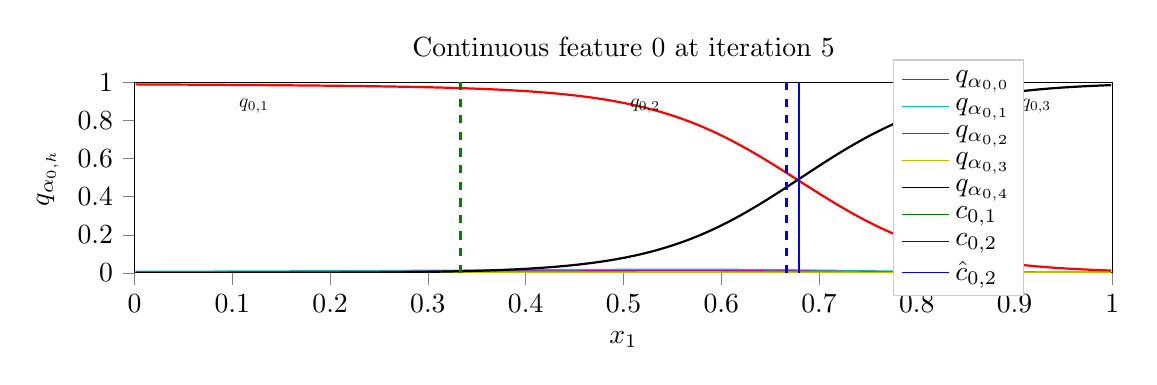
\begin{tikzpicture}

\definecolor{color0}{rgb}{0,0.75,0.75}
\definecolor{color1}{rgb}{0.75,0,0.75}
\definecolor{color2}{rgb}{0.75,0.75,0}

\begin{axis}[
height=\figureheight,
legend cell align={left},
legend entries={{${q}_{\bm{\alpha}_{0,0}}$},{${q}_{\bm{\alpha}_{0,1}}$},{${q}_{\bm{\alpha}_{0,2}}$},{${q}_{\bm{\alpha}_{0,3}}$},{${q}_{\bm{\alpha}_{0,4}}$},{$c_{0,1}$},{$c_{0,2}$},{$\hat{c}_{0,2}$}},
legend style={at={(0.91,0.5)}, anchor=east, draw=white!80.0!black},
tick align=outside,
tick pos=left,
title={Continuous feature 0 at iteration 5},
width=\figurewidth,
x grid style={white!69.01960784313725!black},
xlabel={$x_1$},
xmin=0, xmax=1,
y grid style={white!69.01960784313725!black},
ylabel={${q}_{\bm{\alpha}_{0,h}}$},
ymin=0, ymax=1
]
\addlegendimage{no markers, red}
\addlegendimage{no markers, color0}
\addlegendimage{no markers, color1}
\addlegendimage{no markers, color2}
\addlegendimage{no markers, black}
\addlegendimage{no markers, green!50.0!black}
\addlegendimage{no markers, blue}
\addlegendimage{no markers, blue}
\addplot [thick, red]
table [row sep=\\]{%
0.0011059794751318	0.990096211433411 \\
0.00144600828615515	0.990088164806366 \\
0.00151620394328711	0.990086495876312 \\
0.00161381928831428	0.990084171295166 \\
0.00193644961641948	0.99007648229599 \\
0.0024363370221504	0.990064680576324 \\
0.00384167794354173	0.990030884742737 \\
0.00421063900202368	0.990022242069244 \\
0.00632372037002726	0.989971518516541 \\
0.00947686783375368	0.989895045757294 \\
0.0099356428556221	0.989883720874786 \\
0.0101317191976503	0.989879012107849 \\
0.0102519961026396	0.989876091480255 \\
0.0116572936797861	0.989841759204865 \\
0.0122763055741271	0.989826560020447 \\
0.0128807282915644	0.989811718463898 \\
0.0131006826676461	0.989806354045868 \\
0.0132105085232722	0.989803791046143 \\
0.0150477352877949	0.989758253097534 \\
0.0151511241047927	0.989755690097809 \\
0.0168553495563415	0.989713549613953 \\
0.0191895991753259	0.989655137062073 \\
0.0192724193499449	0.989653170108795 \\
0.0202131188025382	0.989629566669464 \\
0.0251886934986562	0.989503502845764 \\
0.0255409812646521	0.989494621753693 \\
0.0256196546755231	0.989492535591125 \\
0.0263800727822662	0.989473164081573 \\
0.026825697968402	0.989461719989777 \\
0.0272388337061176	0.989451229572296 \\
0.0276781997826389	0.989439904689789 \\
0.0277969734855988	0.989436745643616 \\
0.027888291941232	0.98943430185318 \\
0.032801074197002	0.989307105541229 \\
0.0337126623182875	0.989283204078674 \\
0.0349109578825388	0.989251792430878 \\
0.0367757145561887	0.989202558994293 \\
0.0368887253476963	0.989199638366699 \\
0.0376301111814882	0.989180088043213 \\
0.0383020767002249	0.989162087440491 \\
0.0385765124363792	0.989154756069183 \\
0.0386281055032889	0.989153444766998 \\
0.0397134557815922	0.989124536514282 \\
0.0400530872540832	0.989115476608276 \\
0.0408224228009035	0.989094793796539 \\
0.042416614098386	0.989051878452301 \\
0.042542997860721	0.989048600196838 \\
0.0425634328976269	0.989048182964325 \\
0.0426938593122377	0.989044547080994 \\
0.0436353215690566	0.989019095897675 \\
0.0476491609572692	0.988909900188446 \\
0.0476764809468383	0.988909184932709 \\
0.0480632979275277	0.988898575305939 \\
0.0489335324060199	0.988874673843384 \\
0.0494953541501341	0.988859176635742 \\
0.0498656975684827	0.988848924636841 \\
0.0507299142819697	0.988825023174286 \\
0.0520149216066462	0.988789319992065 \\
0.053491737186121	0.98874819278717 \\
0.0545456118282759	0.988718867301941 \\
0.0549368100196436	0.988707900047302 \\
0.0549667939602374	0.988706946372986 \\
0.0555159955251522	0.988691568374634 \\
0.0574839546417889	0.988636016845703 \\
0.0576927502423773	0.988630056381226 \\
0.0580609228746025	0.988619565963745 \\
0.0610070220733733	0.988535583019257 \\
0.0613718310828713	0.988525211811066 \\
0.0624819644863142	0.988493263721466 \\
0.0632024977130776	0.988472521305084 \\
0.0641707318537266	0.988444447517395 \\
0.064803290117067	0.988426208496094 \\
0.0661546388560771	0.988386809825897 \\
0.0675945492445934	0.988344788551331 \\
0.0701208744758773	0.988270401954651 \\
0.0704495440664726	0.988260746002197 \\
0.0707913481046274	0.988250613212585 \\
0.0709503961374458	0.988245725631714 \\
0.0723079949898875	0.988205313682556 \\
0.0729582139062805	0.988186001777649 \\
0.0736427592129116	0.988165497779846 \\
0.0738431652021745	0.988159537315369 \\
0.074094042941424	0.988152086734772 \\
0.0741988699821797	0.988148748874664 \\
0.0745344402647278	0.988138735294342 \\
0.0761651718345726	0.988089501857758 \\
0.0762565104011357	0.988086819648743 \\
0.0764247618188199	0.988081812858582 \\
0.0780473992355428	0.988032579421997 \\
0.0784939963588281	0.988018870353699 \\
0.0787288834363844	0.988011837005615 \\
0.0796528614743472	0.987983345985413 \\
0.0821291956626848	0.987907350063324 \\
0.0836539892117674	0.987860023975372 \\
0.0837976822096664	0.987855732440948 \\
0.0840863722935196	0.987846791744232 \\
0.0847664004367794	0.987825334072113 \\
0.0848642352310873	0.987822473049164 \\
0.0852150851090396	0.987811505794525 \\
0.085891869345856	0.98779034614563 \\
0.087068315817913	0.987753331661224 \\
0.0885849846877879	0.98770546913147 \\
0.0903431131516136	0.987649619579315 \\
0.0909278592293694	0.987630903720856 \\
0.0914296081009306	0.987614989280701 \\
0.0922298300096035	0.987589418888092 \\
0.0926517333242025	0.987575769424438 \\
0.0930086769471365	0.987564265727997 \\
0.0936368650628759	0.987544059753418 \\
0.0939832817677504	0.987532913684845 \\
0.0963578674192209	0.987455725669861 \\
0.0969604240071604	0.987436056137085 \\
0.0974174263218397	0.987421154975891 \\
0.0997464409700664	0.98734450340271 \\
0.100249930959155	0.987327754497528 \\
0.100820744388044	0.987308919429779 \\
0.101229398304142	0.98729532957077 \\
0.102271393895604	0.987260580062866 \\
0.102325882258744	0.987258732318878 \\
0.103474916599901	0.987220406532288 \\
0.104369461810087	0.987190425395966 \\
0.104849386693897	0.987174034118652 \\
0.105274572558957	0.987159729003906 \\
0.105437385176067	0.987154245376587 \\
0.105718642159513	0.987144768238068 \\
0.106451679001465	0.987119913101196 \\
0.106754108203929	0.987109661102295 \\
0.106889477031479	0.987105011940002 \\
0.108308586301563	0.987056612968445 \\
0.108355506097126	0.987054944038391 \\
0.110864090628752	0.986968576908112 \\
0.112062699234041	0.986927092075348 \\
0.112686863552251	0.986905515193939 \\
0.113787419472266	0.986867070198059 \\
0.114114908535732	0.986855447292328 \\
0.114926076298882	0.98682701587677 \\
0.115710925433917	0.986799418926239 \\
0.116193807044869	0.986782312393188 \\
0.116352662276253	0.986776649951935 \\
0.116979956596317	0.986754596233368 \\
0.117247317403657	0.986745059490204 \\
0.118793828877862	0.986689925193787 \\
0.119352906137166	0.986669838428497 \\
0.120388240876593	0.986632704734802 \\
0.122357154089364	0.986561357975006 \\
0.125712799722249	0.986438751220703 \\
0.126988316690772	0.986391663551331 \\
0.130289689058528	0.986268401145935 \\
0.130830575131366	0.986247956752777 \\
0.13178708265069	0.986211776733398 \\
0.132217070962463	0.98619544506073 \\
0.132641072460891	0.986179351806641 \\
0.133694684584262	0.986139118671417 \\
0.135586813424106	0.986066520214081 \\
0.136970534315695	0.986012995243073 \\
0.137167897059254	0.986005425453186 \\
0.13731957841644	0.985999643802643 \\
0.138770949832641	0.985942959785461 \\
0.141579671494468	0.985832333564758 \\
0.142337772861435	0.985802233219147 \\
0.142852169410084	0.985781610012054 \\
0.14313843453823	0.985770225524902 \\
0.143709892765619	0.985747277736664 \\
0.143996587198751	0.985735833644867 \\
0.144338718134467	0.985722303390503 \\
0.145474509131844	0.985676288604736 \\
0.146058924442183	0.985652804374695 \\
0.147496370200373	0.98559433221817 \\
0.147934500473159	0.985576450824738 \\
0.148464696403164	0.985554695129395 \\
0.149007159183894	0.985532462596893 \\
0.151290695331351	0.985438108444214 \\
0.153507740604538	0.985345423221588 \\
0.153927498261582	0.98532772064209 \\
0.153953160827713	0.985326647758484 \\
0.154179436777791	0.985317170619965 \\
0.155107736993068	0.985277831554413 \\
0.15519005879533	0.985274434089661 \\
0.155418402417591	0.985264718532562 \\
0.156078407887877	0.985236644744873 \\
0.158100170599977	0.98514997959137 \\
0.158283533549941	0.985142171382904 \\
0.158599777942073	0.98512852191925 \\
0.159258263288539	0.985100209712982 \\
0.159678910282026	0.985081911087036 \\
0.162540881855109	0.984956681728363 \\
0.164077384668961	0.984888792037964 \\
0.164957348092599	0.984849691390991 \\
0.165030574098427	0.984846472740173 \\
0.165280388241905	0.984835386276245 \\
0.167273692684132	0.984745621681213 \\
0.168043854724866	0.984710872173309 \\
0.168088628486329	0.984708905220032 \\
0.168662857989897	0.984682738780975 \\
0.169151147716595	0.984660446643829 \\
0.169673214248392	0.984636664390564 \\
0.170135609058708	0.984615385532379 \\
0.171767974673073	0.984540283679962 \\
0.1728518498484	0.984490036964417 \\
0.172984599941167	0.984483897686005 \\
0.176370551959836	0.98432457447052 \\
0.176588273575192	0.984314322471619 \\
0.176656553576852	0.984311044216156 \\
0.17794804219768	0.984249413013458 \\
0.178429717033185	0.984226286411285 \\
0.179458814233081	0.984176635742188 \\
0.180595104426831	0.984121680259705 \\
0.18064479669491	0.984119236469269 \\
0.182294707450728	0.984038591384888 \\
0.182819109355123	0.984012842178345 \\
0.189141614514094	0.983695864677429 \\
0.190723527970293	0.983614504337311 \\
0.192508826701743	0.983521819114685 \\
0.200712508340217	0.983083128929138 \\
0.202130410523186	0.983005046844482 \\
0.202705868873484	0.982973217964172 \\
0.202975660615516	0.982958137989044 \\
0.2033001668374	0.982939958572388 \\
0.204138047670012	0.982893168926239 \\
0.204584283026216	0.982868194580078 \\
0.205975712225296	0.982789635658264 \\
0.208693969096644	0.982634127140045 \\
0.209097012308874	0.982610762119293 \\
0.210129299396579	0.982550919055939 \\
0.210470524326312	0.982531011104584 \\
0.210726758187617	0.982516050338745 \\
0.210879765452585	0.982507050037384 \\
0.213404555935633	0.982357859611511 \\
0.214779680955682	0.982275724411011 \\
0.215976334819965	0.982203483581543 \\
0.21605980843853	0.982198417186737 \\
0.21626681121775	0.982185900211334 \\
0.217333435243771	0.982120931148529 \\
0.217860184045886	0.982088625431061 \\
0.218810300034316	0.982030212879181 \\
0.219036830922259	0.982016265392303 \\
0.219186045259484	0.982006967067719 \\
0.219509161852637	0.981986999511719 \\
0.219517283100912	0.981986403465271 \\
0.220007941128277	0.981955945491791 \\
0.221124031401732	0.981886148452759 \\
0.221655686766872	0.981852829456329 \\
0.222787328400317	0.981781363487244 \\
0.222812240344664	0.981779634952545 \\
0.224413114839207	0.98167759180069 \\
0.225712117798195	0.98159384727478 \\
0.226064824403414	0.981570899486542 \\
0.22778297811216	0.981458723545074 \\
0.227786137279108	0.981458604335785 \\
0.228255816092263	0.981427669525146 \\
0.22886379454373	0.981387257575989 \\
0.229286896531361	0.981359362602234 \\
0.231570483736477	0.981206357479095 \\
0.232839821990075	0.98112028837204 \\
0.234699792231533	0.98099285364151 \\
0.236598748956898	0.980860710144043 \\
0.236914864918852	0.980838418006897 \\
0.238193170258512	0.980748295783997 \\
0.238267801131912	0.980743169784546 \\
0.241280255564163	0.98052704334259 \\
0.241532477911657	0.980508804321289 \\
0.242724887440966	0.980421721935272 \\
0.243487528482621	0.980365574359894 \\
0.243851755033328	0.980338871479034 \\
0.243931127736832	0.980332911014557 \\
0.245492487219521	0.980216801166534 \\
0.245961870318215	0.980181634426117 \\
0.247220233087027	0.980086445808411 \\
0.248029547774932	0.980025112628937 \\
0.248195183805212	0.980012357234955 \\
0.252597476547261	0.97967004776001 \\
0.254049623190913	0.97955459356308 \\
0.254469169693275	0.979520857334137 \\
0.254777550536903	0.9794961810112 \\
0.254877558399671	0.9794881939888 \\
0.257253649731868	0.979295134544373 \\
0.257671137054733	0.979260742664337 \\
0.26187840669548	0.978908538818359 \\
0.264182169008257	0.978710412979126 \\
0.265462287195374	0.978598713874817 \\
0.267638564660905	0.978406071662903 \\
0.268216851612881	0.978354394435883 \\
0.269980014659659	0.978195011615753 \\
0.270837940398052	0.978116631507874 \\
0.271133018969332	0.97808963060379 \\
0.271522794293612	0.978053689002991 \\
0.272730212426688	0.977941691875458 \\
0.27325151773824	0.977893173694611 \\
0.273458501731612	0.977873682975769 \\
0.275787496734588	0.977653026580811 \\
0.275790346826632	0.977652788162231 \\
0.275963502468307	0.977636277675629 \\
0.276441724078765	0.977590441703796 \\
0.277788622824976	0.977460145950317 \\
0.278249554181787	0.977415263652802 \\
0.278902433397602	0.977351307868958 \\
0.280228184178203	0.977220237255096 \\
0.282170737525181	0.977025628089905 \\
0.284775883532131	0.976759314537048 \\
0.285319633849948	0.976702868938446 \\
0.285945143849347	0.976637721061707 \\
0.287293498153222	0.976496040821075 \\
0.288098109983407	0.976410686969757 \\
0.288474372887691	0.976370573043823 \\
0.288733693686359	0.976342856884003 \\
0.291563977198166	0.97603577375412 \\
0.293976605993451	0.975768089294434 \\
0.294014528290392	0.97576367855072 \\
0.294718175832172	0.975684463977814 \\
0.294831463459233	0.975671648979187 \\
0.294887681144015	0.975665271282196 \\
0.299064488228799	0.975183427333832 \\
0.299223468133874	0.975164771080017 \\
0.299853491506122	0.975090265274048 \\
0.301624334890634	0.974878787994385 \\
0.302100714632492	0.974821269512177 \\
0.302855829384862	0.974729657173157 \\
0.303468685820656	0.974654912948608 \\
0.304335545384868	0.97454822063446 \\
0.305081848845274	0.974455714225769 \\
0.305263786725066	0.974433064460754 \\
0.305511643802704	0.974402070045471 \\
0.30635774546767	0.974296033382416 \\
0.307937429467832	0.974095642566681 \\
0.308578187230734	0.974013686180115 \\
0.313991998160918	0.973299562931061 \\
0.315973848719028	0.973028957843781 \\
0.317413649622303	0.97282874584198 \\
0.319657848506035	0.972511410713196 \\
0.319781920771261	0.972493708133698 \\
0.320496004308145	0.972391188144684 \\
0.320601310305949	0.972375869750977 \\
0.322246867517597	0.972136557102203 \\
0.323306124649751	0.971980512142181 \\
0.323664358184811	0.971927285194397 \\
0.323805398711091	0.971906304359436 \\
0.324816846999054	0.971755027770996 \\
0.325263683488062	0.97168755531311 \\
0.327533460856979	0.971340835094452 \\
0.328385869951453	0.971208572387695 \\
0.329844054701458	0.970979809761047 \\
0.33074904970515	0.970836043357849 \\
0.332974695502457	0.970476984977722 \\
0.333600133199531	0.970374703407288 \\
0.336001356191777	0.969975829124451 \\
0.338057278352338	0.969626247882843 \\
0.33940563378102	0.969393193721771 \\
0.339522610836627	0.969372808933258 \\
0.341295751839904	0.969060778617859 \\
0.343025583329651	0.968751013278961 \\
0.344156227439929	0.968545436859131 \\
0.344485478041551	0.968485295772552 \\
0.346631556569637	0.968087196350098 \\
0.348247004908186	0.967781722545624 \\
0.348257869791207	0.967779576778412 \\
0.350134953366802	0.96741795539856 \\
0.352271571140202	0.966997742652893 \\
0.352403536611892	0.966971576213837 \\
0.356607161458692	0.966115713119507 \\
0.357473355861859	0.965934634208679 \\
0.359032837138255	0.965604305267334 \\
0.360085447455855	0.965378224849701 \\
0.360587038984981	0.965269505977631 \\
0.3618814720936	0.964986562728882 \\
0.362541325151431	0.964840710163116 \\
0.363971114014582	0.964521467685699 \\
0.36446377318254	0.964410364627838 \\
0.364734654416428	0.964348793029785 \\
0.364782079325344	0.964338064193726 \\
0.36626622804169	0.96399849653244 \\
0.36745676602671	0.963722169399261 \\
0.367555756327517	0.963698923587799 \\
0.367766921022286	0.963649451732635 \\
0.368015883464081	0.9635910987854 \\
0.368183587302196	0.963551580905914 \\
0.368646745255496	0.963442385196686 \\
0.368824340831231	0.96340024471283 \\
0.36908666014638	0.963337957859039 \\
0.370227788452905	0.963064968585968 \\
0.371079364739364	0.962859034538269 \\
0.371457393668236	0.962767004966736 \\
0.372521553247257	0.96250593662262 \\
0.372816229090882	0.962433159351349 \\
0.373696444358129	0.962214291095734 \\
0.375236418301489	0.961826264858246 \\
0.375355278624935	0.961796045303345 \\
0.375592850161798	0.961735367774963 \\
0.375621310337888	0.961728096008301 \\
0.37623340048021	0.961571455001831 \\
0.376649481158299	0.961464464664459 \\
0.37682934901581	0.96141791343689 \\
0.377022374188538	0.961368024349213 \\
0.378777395062222	0.960908889770508 \\
0.379219181502585	0.960792005062103 \\
0.380639994297166	0.960412204265594 \\
0.381635433931239	0.960142314434052 \\
0.382416367624347	0.959928631782532 \\
0.383276747323035	0.959691107273102 \\
0.383441774868681	0.959645390510559 \\
0.384589480637987	0.959324300289154 \\
0.38762147240542	0.958456873893738 \\
0.387652450706726	0.958447873592377 \\
0.38818745089578	0.95829164981842 \\
0.388531576179462	0.958190679550171 \\
0.391108514236782	0.957422435283661 \\
0.391741157295481	0.957230687141418 \\
0.396723908263121	0.955670952796936 \\
0.39803082540264	0.955247402191162 \\
0.398171926406937	0.955201148986816 \\
0.398666017137866	0.955039083957672 \\
0.398819673578751	0.954988658428192 \\
0.4012576168302	0.954174697399139 \\
0.402752737045505	0.953664541244507 \\
0.403290070599278	0.953479111194611 \\
0.404563584871068	0.953034937381744 \\
0.406532702382757	0.952336013317108 \\
0.406578018270242	0.95231956243515 \\
0.413273296435021	0.949822723865509 \\
0.413592377461711	0.949698925018311 \\
0.41401191876112	0.949535548686981 \\
0.414776267969876	0.949235856533051 \\
0.414785799829368	0.94923210144043 \\
0.415238430177184	0.949053406715393 \\
0.416465974154779	0.948564112186432 \\
0.416689013292801	0.948474586009979 \\
0.418297500020148	0.947821736335754 \\
0.422720878338663	0.945963680744171 \\
0.424343600824592	0.945258438587189 \\
0.425257001696199	0.944855868816376 \\
0.42710227803989	0.944029569625854 \\
0.427962517509508	0.943638324737549 \\
0.429309169026115	0.943018615245819 \\
0.429443446115563	0.942956387996674 \\
0.429705476003957	0.942834436893463 \\
0.431003390699289	0.942225277423859 \\
0.432539042653788	0.941492736339569 \\
0.433068569337496	0.941237270832062 \\
0.433545956268458	0.941005527973175 \\
0.433750136573834	0.94090610742569 \\
0.433778478107147	0.940892279148102 \\
0.434834104829426	0.940374195575714 \\
0.435898870411909	0.939845383167267 \\
0.43750740037395	0.939034342765808 \\
0.437737100851006	0.938917279243469 \\
0.439197385289126	0.93816602230072 \\
0.440921894924801	0.937262892723083 \\
0.442219378180834	0.936571538448334 \\
0.446052885401706	0.934469044208527 \\
0.447759455363191	0.933503150939941 \\
0.448771556188603	0.932921826839447 \\
0.448918332177756	0.932836830615997 \\
0.449861491210787	0.932287991046906 \\
0.449976789412666	0.93222051858902 \\
0.450129821782654	0.932130753993988 \\
0.453058505166632	0.930383682250977 \\
0.455515296612047	0.928872764110565 \\
0.461612686527044	0.924937844276428 \\
0.462183229417738	0.924555659294128 \\
0.46315332653893	0.923900187015533 \\
0.463567773958142	0.923618018627167 \\
0.464569005654222	0.922930955886841 \\
0.46546966357775	0.922306180000305 \\
0.465627783083443	0.922195732593536 \\
0.466166033904132	0.921818792819977 \\
0.466888847202291	0.921308994293213 \\
0.468332203161028	0.920278251171112 \\
0.469094139229819	0.919727563858032 \\
0.469464236056835	0.919458329677582 \\
0.469806075154756	0.919208645820618 \\
0.470776441432414	0.918494880199432 \\
0.471475988022769	0.917975306510925 \\
0.473199954060133	0.916677832603455 \\
0.474832247453521	0.915426313877106 \\
0.475230428162318	0.91511744260788 \\
0.476638306671274	0.914014756679535 \\
0.478988899075304	0.912134945392609 \\
0.479018256118887	0.912111043930054 \\
0.479279919995254	0.911898910999298 \\
0.479532435695615	0.911693453788757 \\
0.479763011578347	0.911505103111267 \\
0.480041882522935	0.911276876926422 \\
0.480923824850651	0.910550653934479 \\
0.481629462985493	0.909964323043823 \\
0.481771508198592	0.90984570980072 \\
0.482503736852496	0.909231722354889 \\
0.483064995688331	0.908757507801056 \\
0.48384062770339	0.908097505569458 \\
0.484085120492796	0.907888293266296 \\
0.484352733912412	0.907658696174622 \\
0.484550939846654	0.907488167285919 \\
0.485022749278845	0.907080709934235 \\
0.485322068953861	0.906821250915527 \\
0.48610300375999	0.906139969825745 \\
0.486253849387163	0.906007766723633 \\
0.489154935058063	0.903421461582184 \\
0.489792628987292	0.902841866016388 \\
0.490458183784177	0.902232706546783 \\
0.492282643359321	0.900540173053741 \\
0.493928358105999	0.898984253406525 \\
0.495701335790147	0.897277057170868 \\
0.496106252426634	0.896882474422455 \\
0.496164487189195	0.89682549238205 \\
0.498739819509518	0.894274115562439 \\
0.500164108812496	0.892832458019257 \\
0.500739446514191	0.89224374294281 \\
0.500830786926564	0.892149984836578 \\
0.502541719930356	0.890376448631287 \\
0.503498564874392	0.889370381832123 \\
0.504534081188611	0.888270020484924 \\
0.504637823699037	0.888159155845642 \\
0.506860898199194	0.885753095149994 \\
0.507491092240963	0.885060489177704 \\
0.508120202534381	0.88436484336853 \\
0.510856303638406	0.881284594535828 \\
0.512327455201249	0.879591703414917 \\
0.51318641739938	0.878591060638428 \\
0.513457954653542	0.878272831439972 \\
0.515863112336536	0.875415325164795 \\
0.516616766484905	0.87450510263443 \\
0.517831355926389	0.873023450374603 \\
0.518931921097757	0.871664762496948 \\
0.521152065672689	0.868876934051514 \\
0.524519468497769	0.864526629447937 \\
0.524576690058109	0.86445140838623 \\
0.525883589956303	0.862721800804138 \\
0.526973717032038	0.861261427402496 \\
0.528680408273136	0.858943045139313 \\
0.530600365407266	0.856287717819214 \\
0.530809662396022	0.855995059013367 \\
0.53166475254574	0.854793667793274 \\
0.532158485575632	0.85409539937973 \\
0.535204926183725	0.849710404872894 \\
0.535356594523575	0.84948867559433 \\
0.537004451507049	0.847058653831482 \\
0.537089668720381	0.846931874752045 \\
0.537190935482585	0.846781194210052 \\
0.538117362047647	0.845395267009735 \\
0.538453506118723	0.844889163970947 \\
0.539359907716354	0.843516826629639 \\
0.539560791003075	0.84321129322052 \\
0.541180326502456	0.840724527835846 \\
0.547271589683928	0.83102285861969 \\
0.548822201570025	0.828463673591614 \\
0.549624872437239	0.8271244764328 \\
0.549819206435189	0.826798737049103 \\
0.550184928091146	0.826184332370758 \\
0.552139674398207	0.822864472866058 \\
0.552982438656419	0.821414768695831 \\
0.5537594353206	0.820068418979645 \\
0.553976139314498	0.819691359996796 \\
0.554051563436848	0.819559931755066 \\
0.55426017856816	0.819195747375488 \\
0.555396555661942	0.817200899124146 \\
0.555501425327998	0.817015826702118 \\
0.556360039382527	0.815493404865265 \\
0.557883446271028	0.812763690948486 \\
0.558670348456701	0.811339199542999 \\
0.559194391744592	0.81038510799408 \\
0.559473603788983	0.809875071048737 \\
0.560198442614008	0.808544635772705 \\
0.560853933269278	0.80733448266983 \\
0.561152915237902	0.806780099868774 \\
0.561401591015197	0.806317985057831 \\
0.562479951006079	0.804302573204041 \\
0.563005908106818	0.803312599658966 \\
0.563050000205171	0.803229629993439 \\
0.563426857102662	0.802517175674438 \\
0.563560604448239	0.802263855934143 \\
0.564062038149409	0.801311492919922 \\
0.565336310962797	0.798872768878937 \\
0.565855772748177	0.797870874404907 \\
0.566858287901599	0.795925199985504 \\
0.566881879040954	0.795879185199738 \\
0.568231608554438	0.793233156204224 \\
0.569223717564581	0.791268885135651 \\
0.569387586449175	0.790942788124084 \\
0.569573989003313	0.790571570396423 \\
0.569720721150053	0.790278792381287 \\
0.572004618116245	0.785676896572113 \\
0.572005154945678	0.785675764083862 \\
0.572151528516064	0.78537791967392 \\
0.57219889974288	0.785281360149384 \\
0.572780347928331	0.784094095230103 \\
0.573600339080632	0.782410204410553 \\
0.576593284261927	0.776169419288635 \\
0.576676798911885	0.775993168354034 \\
0.576819659872325	0.775691270828247 \\
0.577653861143233	0.773922085762024 \\
0.577917937736817	0.773359715938568 \\
0.57793430586259	0.773324608802795 \\
0.581759386894494	0.765045762062073 \\
0.582475032298807	0.763469696044922 \\
0.582896249817215	0.762538135051727 \\
0.589571735768374	0.747377812862396 \\
0.592388904473667	0.740757286548615 \\
0.593611787705259	0.737842679023743 \\
0.594151694891475	0.736547887325287 \\
0.595008948927732	0.734482228755951 \\
0.596105779635777	0.731821835041046 \\
0.597490139381406	0.728435873985291 \\
0.598951438337811	0.724827587604523 \\
0.599201054717089	0.724207758903503 \\
0.600228747033593	0.721645355224609 \\
0.600693928524281	0.720479786396027 \\
0.601589358474053	0.718226373195648 \\
0.602529748251813	0.715845942497253 \\
0.602916831603936	0.714862167835236 \\
0.603866403426713	0.712438344955444 \\
0.606129689323002	0.706603169441223 \\
0.607808363354841	0.702223360538483 \\
0.60811641039762	0.701415002346039 \\
0.608424173673929	0.700605571269989 \\
0.610203299896366	0.695898711681366 \\
0.61052401101773	0.695045053958893 \\
0.611007548691541	0.693754911422729 \\
0.61345268097321	0.687177002429962 \\
0.614300601551049	0.684874773025513 \\
0.616415105925723	0.679087281227112 \\
0.617595625529809	0.675827443599701 \\
0.619695383178102	0.669979572296143 \\
0.620626131680421	0.667367160320282 \\
0.620884093030541	0.666640996932983 \\
0.622959094549987	0.660766005516052 \\
0.624820249131202	0.655446112155914 \\
0.627396892203872	0.648004114627838 \\
0.629679734717881	0.641338348388672 \\
0.63108091324942	0.637214243412018 \\
0.631412061821856	0.636235952377319 \\
0.632209138475077	0.633875846862793 \\
0.632608841524959	0.632689476013184 \\
0.635174872896091	0.625027120113373 \\
0.63680487509045	0.620120048522949 \\
0.638872902814914	0.613851308822632 \\
0.639214862746441	0.61281031370163 \\
0.640549343973947	0.608735322952271 \\
0.6407383188268	0.608156979084015 \\
0.642765742598199	0.601926982402802 \\
0.642772962045468	0.6019047498703 \\
0.644393148200581	0.596896350383759 \\
0.646791193304363	0.589437663555145 \\
0.647126395490269	0.588391005992889 \\
0.647747012654458	0.586449921131134 \\
0.648487744871255	0.584129333496094 \\
0.65164263639371	0.574192881584167 \\
0.651778799711512	0.573762118816376 \\
0.652422089544704	0.57172566652298 \\
0.652778066297422	0.570597231388092 \\
0.653037870316759	0.569773197174072 \\
0.653946378314801	0.566887378692627 \\
0.656181358570071	0.559763491153717 \\
0.657515298781176	0.555495321750641 \\
0.657916355325804	0.554209887981415 \\
0.65821939898974	0.553238093852997 \\
0.660347901626978	0.54639595746994 \\
0.663462409580861	0.536340057849884 \\
0.665002009135555	0.531352043151855 \\
0.665125585501828	0.530951082706451 \\
0.665840946327609	0.528629779815674 \\
0.669598702136104	0.516403913497925 \\
0.669671107753933	0.516167879104614 \\
0.670317902411108	0.514058887958527 \\
0.67055566811489	0.513283312320709 \\
0.670890712943537	0.512190341949463 \\
0.671190867447461	0.51121062040329 \\
0.672572121540986	0.506700158119202 \\
0.674425718831603	0.500641465187073 \\
0.67545414417829	0.497277617454529 \\
0.67596832728122	0.495595216751099 \\
0.676862814397186	0.492667943239212 \\
0.677008756097011	0.492190420627594 \\
0.677760880297266	0.489728361368179 \\
0.680496299332769	0.480773240327835 \\
0.6805627271546	0.480555653572083 \\
0.682518497342478	0.474153965711594 \\
0.682667061493577	0.473667800426483 \\
0.683323391450582	0.471520334482193 \\
0.683455311069743	0.471088707447052 \\
0.686099541255968	0.462443053722382 \\
0.686972247003404	0.459592133760452 \\
0.687287921742946	0.458561450242996 \\
0.688979470872378	0.453042447566986 \\
0.689844777380402	0.450222134590149 \\
0.69066753173656	0.447542697191238 \\
0.690924484351316	0.446706414222717 \\
0.691684985973077	0.444232285022736 \\
0.694075688265434	0.436468929052353 \\
0.694253786667502	0.435891538858414 \\
0.696056771003981	0.430054098367691 \\
0.696659969942023	0.42810469865799 \\
0.69712902782289	0.426590025424957 \\
0.697436633040946	0.425597339868546 \\
0.697470314030711	0.425488620996475 \\
0.698295232645012	0.422829121351242 \\
0.698478216988194	0.422239512205124 \\
0.699563853841568	0.418746262788773 \\
0.700079752305739	0.417088478803635 \\
0.700291212685059	0.416409581899643 \\
0.701162742599685	0.413613885641098 \\
0.702327231437584	0.409885942935944 \\
0.702639966218633	0.408886581659317 \\
0.703077231783761	0.407489717006683 \\
0.703198302674555	0.407103270292282 \\
0.703418311750763	0.40640127658844 \\
0.704913184821873	0.401640087366104 \\
0.705985343895602	0.398235261440277 \\
0.70676366586065	0.395769059658051 \\
0.70953480835097	0.387027144432068 \\
0.709597763991885	0.386829346418381 \\
0.710916839332999	0.382691383361816 \\
0.710971707887323	0.382519632577896 \\
0.711527088935361	0.380782157182693 \\
0.711625741549748	0.380473852157593 \\
0.712030078150365	0.379211097955704 \\
0.713838731517111	0.373580664396286 \\
0.71495171630821	0.370131552219391 \\
0.715877253359645	0.367272347211838 \\
0.717907954554698	0.361029505729675 \\
0.718267373832691	0.359928876161575 \\
0.719482266109768	0.356219351291656 \\
0.720072506203388	0.354422748088837 \\
0.72063303964824	0.35272017121315 \\
0.721414113641739	0.350353419780731 \\
0.721834558021562	0.349082291126251 \\
0.721858215436245	0.349010795354843 \\
0.722606600061919	0.346753358840942 \\
0.723634632256085	0.343662649393082 \\
0.724295951475884	0.341681331396103 \\
0.724780388322819	0.340233087539673 \\
0.725967182906895	0.336696922779083 \\
0.728562998007155	0.329022765159607 \\
0.729378939538106	0.326628237962723 \\
0.729672766087416	0.325767874717712 \\
0.730156271089799	0.324354827404022 \\
0.730418624607748	0.323589235544205 \\
0.731079272213317	0.321665316820145 \\
0.73140958111192	0.320705652236938 \\
0.734582373950397	0.311561495065689 \\
0.735036686489948	0.310263335704803 \\
0.736495162798249	0.306115239858627 \\
0.737637169481189	0.302887976169586 \\
0.738132551177952	0.301493614912033 \\
0.738772404713377	0.299698114395142 \\
0.73919080617973	0.29852694272995 \\
0.739634766317876	0.297287374734879 \\
0.739671405613807	0.297185093164444 \\
0.740318229014976	0.29538431763649 \\
0.741017797721675	0.293443560600281 \\
0.741923938399663	0.290940582752228 \\
0.742870439596604	0.288338959217072 \\
0.743500813750507	0.286613702774048 \\
0.745235425982657	0.281897068023682 \\
0.745794924415534	0.280385494232178 \\
0.746651135832285	0.278081715106964 \\
0.748242417565033	0.273829787969589 \\
0.749080152481028	0.27160707116127 \\
0.750738597109713	0.267239719629288 \\
0.754059260293618	0.258626043796539 \\
0.754427277039572	0.257682293653488 \\
0.755971311279052	0.253746628761292 \\
0.7564660147832	0.252493858337402 \\
0.756964107658398	0.25123655796051 \\
0.757301980310619	0.250385910272598 \\
0.757561417579673	0.249734044075012 \\
0.759460973532791	0.244995072484016 \\
0.759943823499425	0.243799924850464 \\
0.76007481161266	0.243476375937462 \\
0.76520949758525	0.231018230319023 \\
0.769369251223668	0.22125019133091 \\
0.77094746139779	0.217620730400085 \\
0.771797041083953	0.21568451821804 \\
0.772164013593626	0.214852020144463 \\
0.772721858147557	0.213590756058693 \\
0.774553209660584	0.209487617015839 \\
0.774686774792601	0.209190681576729 \\
0.774763255366	0.209020838141441 \\
0.776676196809448	0.204802736639977 \\
0.781826328102722	0.193756580352783 \\
0.783936140597273	0.189361944794655 \\
0.784010287514813	0.189208775758743 \\
0.784889735175701	0.187400385737419 \\
0.785018616770813	0.18713641166687 \\
0.78602927274531	0.185076639056206 \\
0.786818186718577	0.183480724692345 \\
0.787974469502378	0.181160762906075 \\
0.791139177359944	0.174926340579987 \\
0.791586708117001	0.174058318138123 \\
0.791796196079504	0.173653185367584 \\
0.79182158322754	0.173604100942612 \\
0.792072748806228	0.173119336366653 \\
0.792682852079258	0.171946510672569 \\
0.792705401732446	0.171903118491173 \\
0.794569839509874	0.168357774615288 \\
0.795023193386171	0.167504355311394 \\
0.795367478837485	0.166858613491058 \\
0.795527938976809	0.166558355093002 \\
0.795634872431087	0.166358456015587 \\
0.79745955888423	0.162976890802383 \\
0.798224122257701	0.161576196551323 \\
0.799881016007139	0.158573821187019 \\
0.801765379467602	0.155213922262192 \\
0.80362962295172	0.151946619153023 \\
0.803814553638313	0.151625588536263 \\
0.806469107208753	0.147077634930611 \\
0.806697504962046	0.146691605448723 \\
0.807337366299355	0.145614445209503 \\
0.808888043138527	0.143031120300293 \\
0.809190014741277	0.142532423138618 \\
0.809307640373056	0.142338573932648 \\
0.810501764417227	0.140382960438728 \\
0.811889729396757	0.138137951493263 \\
0.811942350832027	0.138053387403488 \\
0.814196326909986	0.134472921490669 \\
0.815151250895423	0.132979646325111 \\
0.815544311745005	0.132369130849838 \\
0.816375455024602	0.131085768342018 \\
0.818069790025891	0.128501832485199 \\
0.820698196177955	0.124578781425953 \\
0.821263012964588	0.123749099671841 \\
0.823441468430582	0.12059336155653 \\
0.824103550036923	0.119648009538651 \\
0.825253713607837	0.118020720779896 \\
0.827170035611177	0.115351937711239 \\
0.827687372625058	0.114640332758427 \\
0.828681002627947	0.113284409046173 \\
0.831688136352904	0.10926491767168 \\
0.832015103492291	0.10883554071188 \\
0.832618539764885	0.108046777546406 \\
0.833979270360146	0.106286577880383 \\
0.835071309810646	0.104892037808895 \\
0.835699577265585	0.104097053408623 \\
0.836498037763016	0.103094324469566 \\
0.836836957998254	0.102671273052692 \\
0.838046127292981	0.101174354553223 \\
0.838525323246066	0.100586548447609 \\
0.839239765753767	0.0997155755758286 \\
0.839402685897079	0.0995179638266563 \\
0.839999299682593	0.0987970679998398 \\
0.840281951751549	0.0984571576118469 \\
0.840483203711437	0.0982158184051514 \\
0.840691788412589	0.0979661270976067 \\
0.842685722208791	0.0956081002950668 \\
0.842993851211431	0.0952482372522354 \\
0.844759374999568	0.0932093486189842 \\
0.844835827371022	0.0931220427155495 \\
0.844992041004939	0.0929436609148979 \\
0.84621071404422	0.0915626734495163 \\
0.84647818555566	0.0912620201706886 \\
0.847551016932997	0.0900650173425674 \\
0.848091115090324	0.0894677713513374 \\
0.84863665263528	0.0888680964708328 \\
0.85175414414149	0.0855099707841873 \\
0.852055625215632	0.0851913616061211 \\
0.853183518340707	0.0840088054537773 \\
0.855762763379044	0.0813601985573769 \\
0.855845256518328	0.0812767520546913 \\
0.856101518575613	0.0810180678963661 \\
0.856353280691239	0.080764576792717 \\
0.857431392977156	0.0796872824430466 \\
0.858507268631162	0.0786252692341805 \\
0.858727032795181	0.0784099102020264 \\
0.859611972462117	0.0775482207536697 \\
0.860598063349272	0.0765981748700142 \\
0.861479766548793	0.0757577568292618 \\
0.863021652496581	0.0743081793189049 \\
0.863191163941701	0.0741504058241844 \\
0.863243196088782	0.0741020143032074 \\
0.863264684077014	0.0740820914506912 \\
0.86433033865504	0.0730978772044182 \\
0.865386426798682	0.072134368121624 \\
0.865574805896198	0.0719637870788574 \\
0.867009964664233	0.0706759169697762 \\
0.868402477420643	0.0694465637207031 \\
0.868462536448662	0.0693939700722694 \\
0.8687736544668	0.0691222622990608 \\
0.870769922748437	0.0674017891287804 \\
0.87137568194098	0.0668875798583031 \\
0.871475162483056	0.066803477704525 \\
0.872823623463892	0.0656731948256493 \\
0.873231322955811	0.0653348714113235 \\
0.87330913025223	0.0652705356478691 \\
0.874554061243274	0.0642485767602921 \\
0.874752616263773	0.0640869736671448 \\
0.875835647990412	0.0632120370864868 \\
0.878375805455995	0.0612033754587173 \\
0.879016462457315	0.060706228017807 \\
0.879915986267341	0.0600145347416401 \\
0.880187041340505	0.0598075799643993 \\
0.880228906915535	0.0597756505012512 \\
0.880706157108953	0.0594130419194698 \\
0.881313907623959	0.0589542053639889 \\
0.88357711634013	0.0572745576500893 \\
0.88575628070969	0.0556997396051884 \\
0.885860150516388	0.0556256771087646 \\
0.885973756819001	0.055544774979353 \\
0.886578379643548	0.0551162138581276 \\
0.88662976023068	0.0550799295306206 \\
0.887201064437371	0.054678063839674 \\
0.88721221948908	0.0546702556312084 \\
0.889489342121342	0.0530958771705627 \\
0.889610563902722	0.0530132614076138 \\
0.891226627532086	0.0519235245883465 \\
0.891601333881282	0.0516739264130592 \\
0.894395711960869	0.0498476177453995 \\
0.894941283658575	0.049498226493597 \\
0.895002834569702	0.0494589321315289 \\
0.895316145165804	0.0492595136165619 \\
0.89572498422586	0.0490003749728203 \\
0.900281097465164	0.0461988039314747 \\
0.901776757070804	0.0453127138316631 \\
0.902902077475763	0.0446566566824913 \\
0.903042041253622	0.0445757023990154 \\
0.903417484940991	0.044359240680933 \\
0.905006674071476	0.043453898280859 \\
0.905428107857581	0.0432167798280716 \\
0.90623158203924	0.0427681431174278 \\
0.909863735264334	0.0407948344945908 \\
0.914192347433306	0.0385566279292107 \\
0.914860066850241	0.0382219776511192 \\
0.916826528028795	0.0372525826096535 \\
0.918089828672593	0.036642350256443 \\
0.918205626409754	0.0365868918597698 \\
0.918453743387651	0.0364683046936989 \\
0.918779069418784	0.0363134145736694 \\
0.919195929572793	0.0361158698797226 \\
0.920730394218805	0.0353975892066956 \\
0.920881992386684	0.0353273823857307 \\
0.921716310403637	0.034943301230669 \\
0.921720421578646	0.0349414348602295 \\
0.923498857953819	0.0341362096369267 \\
0.923553028604257	0.0341119728982449 \\
0.924006080008399	0.0339098572731018 \\
0.92420639372191	0.0338208824396133 \\
0.924470669810756	0.033703800290823 \\
0.924724469351036	0.0335917286574841 \\
0.926231702262142	0.0329335816204548 \\
0.926990949332903	0.0326067730784416 \\
0.933531060787661	0.0299183428287506 \\
0.934434631069947	0.029564194381237 \\
0.934570551019964	0.0295112747699022 \\
0.935534942058006	0.0291384011507034 \\
0.936268298594132	0.0288579314947128 \\
0.936269242169234	0.0288575738668442 \\
0.938329910665083	0.0280833467841148 \\
0.94030185596857	0.0273613706231117 \\
0.940807389024333	0.0271792020648718 \\
0.941016354925932	0.0271042343229055 \\
0.942120305962364	0.0267115645110607 \\
0.944292950605489	0.02595479413867 \\
0.944561491811014	0.025862742215395 \\
0.944673077956372	0.0258245673030615 \\
0.945708241295843	0.0254731141030788 \\
0.947179815483775	0.0249814670532942 \\
0.947693224914561	0.024812113493681 \\
0.950107910712063	0.0240305103361607 \\
0.953012070755755	0.0231222026050091 \\
0.953264426846652	0.0230448730289936 \\
0.953432175112961	0.0229936074465513 \\
0.954059232722306	0.0228029489517212 \\
0.954894864067499	0.0225512962788343 \\
0.955427443299792	0.0223923027515411 \\
0.958107244064232	0.021608853712678 \\
0.95825981412274	0.0215650480240583 \\
0.961834544341432	0.0205634534358978 \\
0.962013308437074	0.0205145832151175 \\
0.962557230525089	0.0203665737062693 \\
0.964107437971182	0.0199504364281893 \\
0.96546229210349	0.0195935647934675 \\
0.966544858040119	0.0193128902465105 \\
0.966587760026518	0.0193018466234207 \\
0.966792601928706	0.0192492213100195 \\
0.968404850237238	0.018839854747057 \\
0.968813010049556	0.0187375675886869 \\
0.969045613941432	0.018679516389966 \\
0.969871084100612	0.0184749495238066 \\
0.970530837594512	0.0183130577206612 \\
0.971272888982341	0.0181325878947973 \\
0.971527190360033	0.0180711448192596 \\
0.977559419065177	0.0166721772402525 \\
0.978837143824273	0.0163897853344679 \\
0.979500241452307	0.0162451043725014 \\
0.979698366054342	0.0162021163851023 \\
0.981925106253984	0.0157265737652779 \\
0.98193841332347	0.0157237946987152 \\
0.985466980517735	0.0149983437731862 \\
0.985624420362111	0.0149667505174875 \\
0.985660230866112	0.0149595765396953 \\
0.985903288996567	0.0149109559133649 \\
0.986891736095765	0.0147148352116346 \\
0.988177000983844	0.014463622123003 \\
0.988188066807458	0.0144614763557911 \\
0.988339255736614	0.0144322160631418 \\
0.988532835659511	0.0143948271870613 \\
0.988627149659547	0.0143766487017274 \\
0.991317832181511	0.0138673530891538 \\
0.991792763797732	0.0137793282046914 \\
0.99271508471038	0.0136099439114332 \\
0.992808132462744	0.0135929780080914 \\
0.99282017193431	0.0135907810181379 \\
0.994749345227338	0.0132435532286763 \\
0.99866338972896	0.0125657673925161 \\
};
\addplot [thick, color0]
table [row sep=\\]{%
0.0011059794751318	0.00577228888869286 \\
0.00144600828615515	0.0057767303660512 \\
0.00151620394328711	0.00577764911577106 \\
0.00161381928831428	0.005778927821666 \\
0.00193644961641948	0.00578314997255802 \\
0.0024363370221504	0.00578969763591886 \\
0.00384167794354173	0.00580814201384783 \\
0.00421063900202368	0.00581299560144544 \\
0.00632372037002726	0.00584086263552308 \\
0.00947686783375368	0.00588269112631679 \\
0.0099356428556221	0.00588879827409983 \\
0.0101317191976503	0.00589141016826034 \\
0.0102519961026396	0.00589301669970155 \\
0.0116572936797861	0.00591178191825747 \\
0.0122763055741271	0.0059200688265264 \\
0.0128807282915644	0.0059281699359417 \\
0.0131006826676461	0.0059311231598258 \\
0.0132105085232722	0.00593259884044528 \\
0.0150477352877949	0.00595731055364013 \\
0.0151511241047927	0.00595870427787304 \\
0.0168553495563415	0.00598172284662724 \\
0.0191895991753259	0.00601339060813189 \\
0.0192724193499449	0.00601451983675361 \\
0.0202131188025382	0.00602733623236418 \\
0.0251886934986562	0.00609554909169674 \\
0.0255409812646521	0.00610040547326207 \\
0.0256196546755231	0.00610149558633566 \\
0.0263800727822662	0.00611199252307415 \\
0.026825697968402	0.00611815927550197 \\
0.0272388337061176	0.00612387619912624 \\
0.0276781997826389	0.00612996472045779 \\
0.0277969734855988	0.00613161409273744 \\
0.027888291941232	0.00613287696614861 \\
0.032801074197002	0.00620138738304377 \\
0.0337126623182875	0.00621418794617057 \\
0.0349109578825388	0.00623104581609368 \\
0.0367757145561887	0.0062573654577136 \\
0.0368887253476963	0.00625896407291293 \\
0.0376301111814882	0.00626946799457073 \\
0.0383020767002249	0.00627899635583162 \\
0.0385765124363792	0.00628289440646768 \\
0.0386281055032889	0.00628362316638231 \\
0.0397134557815922	0.00629906309768558 \\
0.0400530872540832	0.00630389992147684 \\
0.0408224228009035	0.00631487229838967 \\
0.042416614098386	0.00633766874670982 \\
0.042542997860721	0.00633947970345616 \\
0.0425634328976269	0.00633977307006717 \\
0.0426938593122377	0.00634163990616798 \\
0.0436353215690566	0.00635514641180634 \\
0.0476491609572692	0.00641306024044752 \\
0.0476764809468383	0.00641345605254173 \\
0.0480632979275277	0.00641906587406993 \\
0.0489335324060199	0.00643169926479459 \\
0.0494953541501341	0.00643987162038684 \\
0.0498656975684827	0.00644526071846485 \\
0.0507299142819697	0.00645785918459296 \\
0.0520149216066462	0.00647663464769721 \\
0.053491737186121	0.00649828230962157 \\
0.0545456118282759	0.00651377113536 \\
0.0549368100196436	0.006519531365484 \\
0.0549667939602374	0.00651996955275536 \\
0.0555159955251522	0.0065280687995255 \\
0.0574839546417889	0.00655715120956302 \\
0.0576927502423773	0.00656024552881718 \\
0.0580609228746025	0.00656570261344314 \\
0.0610070220733733	0.00660953437909484 \\
0.0613718310828713	0.00661498587578535 \\
0.0624819644863142	0.0066315894946456 \\
0.0632024977130776	0.00664239097386599 \\
0.0641707318537266	0.0066569303162396 \\
0.064803290117067	0.00666644796729088 \\
0.0661546388560771	0.00668681552633643 \\
0.0675945492445934	0.00670859590172768 \\
0.0701208744758773	0.0067469677887857 \\
0.0704495440664726	0.00675197783857584 \\
0.0707913481046274	0.00675718672573566 \\
0.0709503961374458	0.00675961282104254 \\
0.0723079949898875	0.00678036082535982 \\
0.0729582139062805	0.00679031992331147 \\
0.0736427592129116	0.00680082337930799 \\
0.0738431652021745	0.00680389627814293 \\
0.074094042941424	0.00680775195360184 \\
0.0741988699821797	0.00680935895070434 \\
0.0745344402647278	0.00681452266871929 \\
0.0761651718345726	0.00683964928612113 \\
0.0762565104011357	0.00684105977416039 \\
0.0764247618188199	0.00684365490451455 \\
0.0780473992355428	0.00686876149848104 \\
0.0784939963588281	0.00687569146975875 \\
0.0787288834363844	0.00687933573499322 \\
0.0796528614743472	0.00689369719475508 \\
0.0821291956626848	0.00693231960758567 \\
0.0836539892117674	0.00695620849728584 \\
0.0837976822096664	0.00695846462622285 \\
0.0840863722935196	0.00696299830451608 \\
0.0847664004367794	0.00697368942201138 \\
0.0848642352310873	0.00697522889822721 \\
0.0852150851090396	0.0069807511754334 \\
0.085891869345856	0.00699141481891274 \\
0.087068315817913	0.00700999330729246 \\
0.0885849846877879	0.00703401537612081 \\
0.0903431131516136	0.00706196157261729 \\
0.0909278592293694	0.00707127572968602 \\
0.0914296081009306	0.00707928603515029 \\
0.0922298300096035	0.00709207309409976 \\
0.0926517333242025	0.00709882332012057 \\
0.0930086769471365	0.00710454117506742 \\
0.0936368650628759	0.00711461016908288 \\
0.0939832817677504	0.00712016690522432 \\
0.0963578674192209	0.00715839024633169 \\
0.0969604240071604	0.00716812256723642 \\
0.0974174263218397	0.00717551400884986 \\
0.0997464409700664	0.00721327820792794 \\
0.100249930959155	0.00722147058695555 \\
0.100820744388044	0.00723076984286308 \\
0.101229398304142	0.0072374283336103 \\
0.102271393895604	0.00725444545969367 \\
0.102325882258744	0.00725533813238144 \\
0.103474916599901	0.0072741499170661 \\
0.104369461810087	0.00728882802650332 \\
0.104849386693897	0.00729671493172646 \\
0.105274572558957	0.00730370730161667 \\
0.105437385176067	0.00730638718232512 \\
0.105718642159513	0.0073110219091177 \\
0.106451679001465	0.00732310535386205 \\
0.106754108203929	0.00732809724286199 \\
0.106889477031479	0.0073303310200572 \\
0.108308586301563	0.00735380547121167 \\
0.108355506097126	0.0073545821942389 \\
0.110864090628752	0.00739626213908195 \\
0.112062699234041	0.00741625390946865 \\
0.112686863552251	0.00742668705061078 \\
0.113787419472266	0.0074451151303947 \\
0.114114908535732	0.00745061039924622 \\
0.114926076298882	0.00746423518285155 \\
0.115710925433917	0.00747743900865316 \\
0.116193807044869	0.0074855680577457 \\
0.116352662276253	0.00748824886977673 \\
0.116979956596317	0.00749883288517594 \\
0.117247317403657	0.00750334979966283 \\
0.118793828877862	0.00752951996400952 \\
0.119352906137166	0.00753900222480297 \\
0.120388240876593	0.00755659071728587 \\
0.122357154089364	0.00759015558287501 \\
0.125712799722249	0.00764768850058317 \\
0.126988316690772	0.00766966911032796 \\
0.130289689058528	0.00772684486582875 \\
0.130830575131366	0.00773624749854207 \\
0.13178708265069	0.00775291072204709 \\
0.132217070962463	0.00776041299104691 \\
0.132641072460891	0.00776781560853124 \\
0.133694684584262	0.00778624089434743 \\
0.135586813424106	0.00781943555921316 \\
0.136970534315695	0.0078437989577651 \\
0.137167897059254	0.00784728582948446 \\
0.13731957841644	0.00784996058791876 \\
0.138770949832641	0.00787561479955912 \\
0.141579671494468	0.00792548805475235 \\
0.142337772861435	0.0079390024766326 \\
0.142852169410084	0.00794818066060543 \\
0.14313843453823	0.00795329827815294 \\
0.143709892765619	0.0079635176807642 \\
0.143996587198751	0.00796864461153746 \\
0.144338718134467	0.00797477271407843 \\
0.145474509131844	0.00799514725804329 \\
0.146058924442183	0.00800565350800753 \\
0.147496370200373	0.00803154241293669 \\
0.147934500473159	0.00803945306688547 \\
0.148464696403164	0.00804902613162994 \\
0.149007159183894	0.00805884134024382 \\
0.151290695331351	0.00810027401894331 \\
0.153507740604538	0.00814068969339132 \\
0.153927498261582	0.00814836099743843 \\
0.153953160827713	0.00814883410930634 \\
0.154179436777791	0.00815297290682793 \\
0.155107736993068	0.00816997699439526 \\
0.15519005879533	0.00817149132490158 \\
0.155418402417591	0.00817567855119705 \\
0.156078407887877	0.00818780157715082 \\
0.158100170599977	0.00822502840310335 \\
0.158283533549941	0.00822841562330723 \\
0.158599777942073	0.00823425222188234 \\
0.159258263288539	0.00824642740190029 \\
0.159678910282026	0.00825421698391438 \\
0.162540881855109	0.00830737501382828 \\
0.164077384668961	0.00833604950457811 \\
0.164957348092599	0.00835250876843929 \\
0.165030574098427	0.008353884331882 \\
0.165280388241905	0.00835856329649687 \\
0.167273692684132	0.00839599594473839 \\
0.168043854724866	0.00841050874441862 \\
0.168088628486329	0.00841135066002607 \\
0.168662857989897	0.008422183804214 \\
0.169151147716595	0.00843140762299299 \\
0.169673214248392	0.00844127777963877 \\
0.170135609058708	0.00845002755522728 \\
0.171767974673073	0.0084809921681881 \\
0.1728518498484	0.00850160978734493 \\
0.172984599941167	0.00850414019078016 \\
0.176370551959836	0.00856887456029654 \\
0.176588273575192	0.00857305619865656 \\
0.176656553576852	0.00857436470687389 \\
0.17794804219768	0.00859919749200344 \\
0.178429717033185	0.00860847253352404 \\
0.179458814233081	0.00862833019345999 \\
0.180595104426831	0.00865029916167259 \\
0.18064479669491	0.00865125935524702 \\
0.182294707450728	0.00868326518684626 \\
0.182819109355123	0.00869345758110285 \\
0.189141614514094	0.00881726294755936 \\
0.190723527970293	0.00884849112480879 \\
0.192508826701743	0.00888386182487011 \\
0.200712508340217	0.00904811266809702 \\
0.202130410523186	0.00907678995281458 \\
0.202705868873484	0.00908844918012619 \\
0.202975660615516	0.00909391883760691 \\
0.2033001668374	0.00910050515085459 \\
0.204138047670012	0.00911752879619598 \\
0.204584283026216	0.00912661384791136 \\
0.205975712225296	0.0091549726203084 \\
0.208693969096644	0.00921061728149652 \\
0.209097012308874	0.00921889673918486 \\
0.210129299396579	0.00924012809991837 \\
0.210470524326312	0.00924715213477612 \\
0.210726758187617	0.00925243645906448 \\
0.210879765452585	0.00925558991730213 \\
0.213404555935633	0.00930778589099646 \\
0.214779680955682	0.00933632627129555 \\
0.215976334819965	0.00936122704297304 \\
0.21605980843853	0.00936296954751015 \\
0.21626681121775	0.00936728436499834 \\
0.217333435243771	0.00938954763114452 \\
0.217860184045886	0.0094005586579442 \\
0.218810300034316	0.00942045170813799 \\
0.219036830922259	0.00942520145326853 \\
0.219186045259484	0.00942833069711924 \\
0.219509161852637	0.00943510606884956 \\
0.219517283100912	0.00943528115749359 \\
0.220007941128277	0.00944558344781399 \\
0.221124031401732	0.0094690565019846 \\
0.221655686766872	0.00948025472462177 \\
0.222787328400317	0.00950413756072521 \\
0.222812240344664	0.00950466003268957 \\
0.224413114839207	0.00953853968530893 \\
0.225712117798195	0.00956611055880785 \\
0.226064824403414	0.00957360304892063 \\
0.22778297811216	0.00961020775139332 \\
0.227786137279108	0.00961027666926384 \\
0.228255816092263	0.00962030328810215 \\
0.22886379454373	0.00963329710066319 \\
0.229286896531361	0.0096423514187336 \\
0.231570483736477	0.00969134271144867 \\
0.232839821990075	0.00971866399049759 \\
0.234699792231533	0.00975883472710848 \\
0.236598748956898	0.00979999452829361 \\
0.236914864918852	0.00980685837566853 \\
0.238193170258512	0.00983467604964972 \\
0.238267801131912	0.00983630958944559 \\
0.241280255564163	0.00990213546901941 \\
0.241532477911657	0.00990766566246748 \\
0.242724887440966	0.00993384886533022 \\
0.243487528482621	0.00995062571018934 \\
0.243851755033328	0.00995864812284708 \\
0.243931127736832	0.00996039714664221 \\
0.245492487219521	0.00999484956264496 \\
0.245961870318215	0.0100052300840616 \\
0.247220233087027	0.0100330924615264 \\
0.248029547774932	0.0100510530173779 \\
0.248195183805212	0.0100547382608056 \\
0.252597476547261	0.0101529518142343 \\
0.254049623190913	0.010185532271862 \\
0.254469169693275	0.0101949628442526 \\
0.254777550536903	0.0102018974721432 \\
0.254877558399671	0.0102041503414512 \\
0.257253649731868	0.0102577386423945 \\
0.257671137054733	0.0102671850472689 \\
0.26187840669548	0.010362739674747 \\
0.264182169008257	0.0104153864085674 \\
0.265462287195374	0.0104447333142161 \\
0.267638564660905	0.0104947928339243 \\
0.268216851612881	0.0105081340298057 \\
0.269980014659659	0.0105488803237677 \\
0.270837940398052	0.0105687575414777 \\
0.271133018969332	0.0105755990371108 \\
0.271522794293612	0.010584644973278 \\
0.272730212426688	0.0106127075850964 \\
0.27325151773824	0.0106248399242759 \\
0.273458501731612	0.0106296604499221 \\
0.275787496734588	0.0106840264052153 \\
0.275790346826632	0.0106840953230858 \\
0.275963502468307	0.0106881437823176 \\
0.276441724078765	0.010699350386858 \\
0.277788622824976	0.0107309278100729 \\
0.278249554181787	0.0107417553663254 \\
0.278902433397602	0.0107571100816131 \\
0.280228184178203	0.0107883308082819 \\
0.282170737525181	0.0108342235907912 \\
0.284775883532131	0.0108960065990686 \\
0.285319633849948	0.0109089408069849 \\
0.285945143849347	0.0109238233417273 \\
0.287293498153222	0.0109559874981642 \\
0.288098109983407	0.0109752118587494 \\
0.288474372887691	0.0109842056408525 \\
0.288733693686359	0.0109904110431671 \\
0.291563977198166	0.0110583202913404 \\
0.293976605993451	0.0111164636909962 \\
0.294014528290392	0.0111173838376999 \\
0.294718175832172	0.0111343860626221 \\
0.294831463459233	0.0111371222883463 \\
0.294887681144015	0.0111384829506278 \\
0.299064488228799	0.011239861138165 \\
0.299223468133874	0.0112437307834625 \\
0.299853491506122	0.0112590901553631 \\
0.301624334890634	0.0113023379817605 \\
0.302100714632492	0.0113139916211367 \\
0.302855829384862	0.0113324895501137 \\
0.303468685820656	0.0113475173711777 \\
0.304335545384868	0.0113687943667173 \\
0.305081848845274	0.0113871367648244 \\
0.305263786725066	0.0113916136324406 \\
0.305511643802704	0.0113977119326591 \\
0.30635774546767	0.0114185493439436 \\
0.307937429467832	0.011457527987659 \\
0.308578187230734	0.0114733688533306 \\
0.313991998160918	0.0116078220307827 \\
0.315973848719028	0.0116573208943009 \\
0.317413649622303	0.0116933761164546 \\
0.319657848506035	0.0117497267201543 \\
0.319781920771261	0.0117528410628438 \\
0.320496004308145	0.0117708155885339 \\
0.320601310305949	0.0117734707891941 \\
0.322246867517597	0.0118149565532804 \\
0.323306124649751	0.0118417209014297 \\
0.323664358184811	0.0118507826700807 \\
0.323805398711091	0.0118543477728963 \\
0.324816846999054	0.0118799563497305 \\
0.325263683488062	0.0118912821635604 \\
0.327533460856979	0.0119489151984453 \\
0.328385869951453	0.011970610357821 \\
0.329844054701458	0.0120077766478062 \\
0.33074904970515	0.0120308762416244 \\
0.332974695502457	0.0120878051966429 \\
0.333600133199531	0.01210383977741 \\
0.336001356191777	0.0121655017137527 \\
0.338057278352338	0.0122184464707971 \\
0.33940563378102	0.0122532481327653 \\
0.339522610836627	0.0122562637552619 \\
0.341295751839904	0.0123021146282554 \\
0.343025583329651	0.0123469457030296 \\
0.344156227439929	0.0123762935400009 \\
0.344485478041551	0.0123848523944616 \\
0.346631556569637	0.0124406833201647 \\
0.348247004908186	0.0124827977269888 \\
0.348257869791207	0.0124830789864063 \\
0.350134953366802	0.0125321112573147 \\
0.352271571140202	0.0125880427658558 \\
0.352403536611892	0.0125914961099625 \\
0.356607161458692	0.0127019071951509 \\
0.357473355861859	0.0127247171476483 \\
0.359032837138255	0.0127658229321241 \\
0.360085447455855	0.0127936052158475 \\
0.360587038984981	0.0128068430349231 \\
0.3618814720936	0.0128410561010242 \\
0.362541325151431	0.0128585137426853 \\
0.363971114014582	0.0128963626921177 \\
0.36446377318254	0.0129094207659364 \\
0.364734654416428	0.0129166012629867 \\
0.364782079325344	0.0129178557544947 \\
0.36626622804169	0.0129572236910462 \\
0.36745676602671	0.0129888327792287 \\
0.367555756327517	0.0129914674907923 \\
0.367766921022286	0.0129970703274012 \\
0.368015883464081	0.0130036855116487 \\
0.368183587302196	0.0130081437528133 \\
0.368646745255496	0.0130204521119595 \\
0.368824340831231	0.0130251739174128 \\
0.36908666014638	0.0130321532487869 \\
0.370227788452905	0.0130625171586871 \\
0.371079364739364	0.0130851808935404 \\
0.371457393668236	0.0130952522158623 \\
0.372521553247257	0.0131236091256142 \\
0.372816229090882	0.0131314685568213 \\
0.373696444358129	0.0131549322977662 \\
0.375236418301489	0.0131960399448872 \\
0.375355278624935	0.0131992120295763 \\
0.375592850161798	0.0132055561989546 \\
0.375621310337888	0.0132063124328852 \\
0.37623340048021	0.01322266086936 \\
0.376649481158299	0.0132337780669332 \\
0.37682934901581	0.0132385846227407 \\
0.377022374188538	0.0132437441498041 \\
0.378777395062222	0.013290673494339 \\
0.379219181502585	0.0133024854585528 \\
0.380639994297166	0.0133405150845647 \\
0.381635433931239	0.0133671732619405 \\
0.382416367624347	0.0133880916982889 \\
0.383276747323035	0.0134111503139138 \\
0.383441774868681	0.0134155778214335 \\
0.384589480637987	0.0134463449940085 \\
0.38762147240542	0.0135276783257723 \\
0.387652450706726	0.0135285127907991 \\
0.38818745089578	0.0135428672656417 \\
0.388531576179462	0.0135521050542593 \\
0.391108514236782	0.0136212967336178 \\
0.391741157295481	0.0136382915079594 \\
0.396723908263121	0.0137721505016088 \\
0.39803082540264	0.0138072660192847 \\
0.398171926406937	0.0138110546395183 \\
0.398666017137866	0.0138243259862065 \\
0.398819673578751	0.0138284545391798 \\
0.4012576168302	0.0138939404860139 \\
0.402752737045505	0.0139340832829475 \\
0.403290070599278	0.0139485104009509 \\
0.404563584871068	0.0139826843515038 \\
0.406532702382757	0.0140355071052909 \\
0.406578018270242	0.0140367168933153 \\
0.413273296435021	0.014215980656445 \\
0.413592377461711	0.0142245087772608 \\
0.41401191876112	0.014235713519156 \\
0.414776267969876	0.0142561253160238 \\
0.414785799829368	0.0142563823610544 \\
0.415238430177184	0.0142684616148472 \\
0.416465974154779	0.0143012078478932 \\
0.416689013292801	0.0143071562051773 \\
0.418297500020148	0.0143500091508031 \\
0.422720878338663	0.0144675290212035 \\
0.424343600824592	0.0145105021074414 \\
0.425257001696199	0.0145346615463495 \\
0.42710227803989	0.0145833762362599 \\
0.427962517509508	0.0146060483530164 \\
0.429309169026115	0.0146414870396256 \\
0.429443446115563	0.014645017683506 \\
0.429705476003957	0.0146518955007195 \\
0.431003390699289	0.0146859716624022 \\
0.432539042653788	0.0147262001410127 \\
0.433068569337496	0.0147400461137295 \\
0.433545956268458	0.0147525183856487 \\
0.433750136573834	0.0147578474134207 \\
0.433778478107147	0.0147585943341255 \\
0.434834104829426	0.0147861214354634 \\
0.435898870411909	0.014813844114542 \\
0.43750740037395	0.0148556269705296 \\
0.437737100851006	0.0148615743964911 \\
0.439197385289126	0.0148993749171495 \\
0.440921894924801	0.0149438735097647 \\
0.442219378180834	0.0149772213771939 \\
0.446052885401706	0.0150752225890756 \\
0.447759455363191	0.0151185467839241 \\
0.448771556188603	0.0151441432535648 \\
0.448918332177756	0.0151478545740247 \\
0.449861491210787	0.0151716424152255 \\
0.449976789412666	0.0151745388284326 \\
0.450129821782654	0.0151783972978592 \\
0.453058505166632	0.0152517799288034 \\
0.455515296612047	0.0153128206729889 \\
0.461612686527044	0.0154621200636029 \\
0.462183229417738	0.0154759231954813 \\
0.46315332653893	0.0154993003234267 \\
0.463567773958142	0.0155092626810074 \\
0.464569005654222	0.0155332610011101 \\
0.46546966357775	0.0155547605827451 \\
0.465627783083443	0.015558528713882 \\
0.466166033904132	0.0155713278800249 \\
0.466888847202291	0.015588459558785 \\
0.468332203161028	0.0156225273385644 \\
0.469094139229819	0.015640415251255 \\
0.469464236056835	0.015649076551199 \\
0.469806075154756	0.0156570579856634 \\
0.470776441432414	0.0156796742230654 \\
0.471475988022769	0.0156959015876055 \\
0.473199954060133	0.0157356467097998 \\
0.474832247453521	0.015772944316268 \\
0.475230428162318	0.0157819893211126 \\
0.476638306671274	0.0158138275146484 \\
0.478988899075304	0.0158663783222437 \\
0.479018256118887	0.0158670358359814 \\
0.479279919995254	0.0158728417009115 \\
0.479532435695615	0.0158784314990044 \\
0.479763011578347	0.0158835276961327 \\
0.480041882522935	0.0158896762877703 \\
0.480923824850651	0.0159090850502253 \\
0.481629462985493	0.0159245170652866 \\
0.481771508198592	0.0159276202321053 \\
0.482503736852496	0.0159435477107763 \\
0.483064995688331	0.0159557163715363 \\
0.48384062770339	0.0159724354743958 \\
0.484085120492796	0.0159776899963617 \\
0.484352733912412	0.0159834399819374 \\
0.484550939846654	0.0159876700490713 \\
0.485022749278845	0.0159977525472641 \\
0.485322068953861	0.0160041321069002 \\
0.48610300375999	0.0160207077860832 \\
0.486253849387163	0.0160238929092884 \\
0.489154935058063	0.0160845369100571 \\
0.489792628987292	0.0160976815968752 \\
0.490458183784177	0.0161113310605288 \\
0.492282643359321	0.0161483585834503 \\
0.493928358105999	0.0161812696605921 \\
0.495701335790147	0.0162161644548178 \\
0.496106252426634	0.0162240471690893 \\
0.496164487189195	0.0162251833826303 \\
0.498739819509518	0.0162746161222458 \\
0.500164108812496	0.0163014065474272 \\
0.500739446514191	0.0163121093064547 \\
0.500830786926564	0.0163138043135405 \\
0.502541719930356	0.0163452196866274 \\
0.503498564874392	0.0163625217974186 \\
0.504534081188611	0.0163810402154922 \\
0.504637823699037	0.0163828823715448 \\
0.506860898199194	0.016421789303422 \\
0.507491092240963	0.0164326261729002 \\
0.508120202534381	0.0164433475583792 \\
0.510856303638406	0.0164889618754387 \\
0.512327455201249	0.0165127646178007 \\
0.51318641739938	0.0165264140814543 \\
0.513457954653542	0.0165306944400072 \\
0.515863112336536	0.0165678132325411 \\
0.516616766484905	0.0165791492909193 \\
0.517831355926389	0.0165971107780933 \\
0.518931921097757	0.0166130438446999 \\
0.521152065672689	0.016644224524498 \\
0.524519468497769	0.0166889578104019 \\
0.524576690058109	0.0166896767914295 \\
0.525883589956303	0.0167061574757099 \\
0.526973717032038	0.0167195256799459 \\
0.528680408273136	0.0167397446930408 \\
0.530600365407266	0.0167614407837391 \\
0.530809662396022	0.0167637411504984 \\
0.53166475254574	0.0167729891836643 \\
0.532158485575632	0.0167782176285982 \\
0.535204926183725	0.0168088134378195 \\
0.535356594523575	0.0168102625757456 \\
0.537004451507049	0.0168254692107439 \\
0.537089668720381	0.0168262366205454 \\
0.537190935482585	0.0168271362781525 \\
0.538117362047647	0.016835231333971 \\
0.538453506118723	0.016838101670146 \\
0.539359907716354	0.0168456453830004 \\
0.539560791003075	0.0168472733348608 \\
0.541180326502456	0.0168599393218756 \\
0.547271589683928	0.0168992169201374 \\
0.548822201570025	0.016907038167119 \\
0.549624872437239	0.0169107280671597 \\
0.549819206435189	0.0169115830212831 \\
0.550184928091146	0.0169131550937891 \\
0.552139674398207	0.016920693218708 \\
0.552982438656419	0.0169234741479158 \\
0.5537594353206	0.0169257875531912 \\
0.553976139314498	0.016926396638155 \\
0.554051563436848	0.0169266052544117 \\
0.55426017856816	0.0169271621853113 \\
0.555396555661942	0.016929879784584 \\
0.555501425327998	0.0169301144778728 \\
0.556360039382527	0.0169317908585072 \\
0.557883446271028	0.0169340223073959 \\
0.558670348456701	0.0169347990304232 \\
0.559194391744592	0.0169351696968079 \\
0.559473603788983	0.0169353205710649 \\
0.560198442614008	0.0169355589896441 \\
0.560853933269278	0.0169355887919664 \\
0.561152915237902	0.0169355403631926 \\
0.561401591015197	0.0169354677200317 \\
0.562479951006079	0.0169348586350679 \\
0.563005908106818	0.0169343817979097 \\
0.563050000205171	0.0169343333691359 \\
0.563426857102662	0.0169339049607515 \\
0.563560604448239	0.0169337391853333 \\
0.564062038149409	0.0169330462813377 \\
0.565336310962797	0.0169307980686426 \\
0.565855772748177	0.0169296693056822 \\
0.566858287901599	0.016927158460021 \\
0.566881879040954	0.0169270914047956 \\
0.568231608554438	0.0169229749590158 \\
0.569223717564581	0.0169194340705872 \\
0.569387586449175	0.0169188044965267 \\
0.569573989003313	0.0169180724769831 \\
0.569720721150053	0.0169174820184708 \\
0.572004618116245	0.0169070698320866 \\
0.572005154945678	0.016907062381506 \\
0.572151528516064	0.0169063191860914 \\
0.57219889974288	0.0169060621410608 \\
0.572780347928331	0.0169029776006937 \\
0.573600339080632	0.0168983433395624 \\
0.576593284261927	0.0168787203729153 \\
0.576676798911885	0.0168781112879515 \\
0.576819659872325	0.0168770551681519 \\
0.577653861143233	0.0168707240372896 \\
0.577917937736817	0.0168686471879482 \\
0.57793430586259	0.0168685205280781 \\
0.581759386894494	0.0168345868587494 \\
0.582475032298807	0.0168274343013763 \\
0.582896249817215	0.0168231017887592 \\
0.589571735768374	0.0167423486709595 \\
0.592388904473667	0.0167013239115477 \\
0.593611787705259	0.0166822113096714 \\
0.594151694891475	0.0166735127568245 \\
0.595008948927732	0.0166593920439482 \\
0.596105779635777	0.0166407451033592 \\
0.597490139381406	0.0166162811219692 \\
0.598951438337811	0.0165893379598856 \\
0.599201054717089	0.0165846161544323 \\
0.600228747033593	0.0165648348629475 \\
0.600693928524281	0.0165556874126196 \\
0.601589358474053	0.0165377501398325 \\
0.602529748251813	0.016518434509635 \\
0.602916831603936	0.0165103431791067 \\
0.603866403426713	0.0164901446551085 \\
0.606129689323002	0.0164399780333042 \\
0.607808363354841	0.0164009351283312 \\
0.60811641039762	0.0163935963064432 \\
0.608424173673929	0.016386216506362 \\
0.610203299896366	0.0163425002247095 \\
0.61052401101773	0.016334431245923 \\
0.611007548691541	0.0163221582770348 \\
0.61345268097321	0.0162580776959658 \\
0.614300601551049	0.016235064715147 \\
0.616415105925723	0.0161759275943041 \\
0.617595625529809	0.0161418057978153 \\
0.619695383178102	0.0160791836678982 \\
0.620626131680421	0.0160506181418896 \\
0.620884093030541	0.0160426143556833 \\
0.622959094549987	0.015976894646883 \\
0.624820249131202	0.0159158725291491 \\
0.627396892203872	0.0158281810581684 \\
0.629679734717881	0.0157473832368851 \\
0.63108091324942	0.0156963430345058 \\
0.631412061821856	0.015684125944972 \\
0.632209138475077	0.0156544633209705 \\
0.632608841524959	0.015639454126358 \\
0.635174872896091	0.015541004948318 \\
0.63680487509045	0.0154765909537673 \\
0.638872902814914	0.0153927784413099 \\
0.639214862746441	0.0153787015005946 \\
0.640549343973947	0.0153231509029865 \\
0.6407383188268	0.0153152076527476 \\
0.642765742598199	0.0152287734672427 \\
0.642772962045468	0.0152284661307931 \\
0.644393148200581	0.0151578281074762 \\
0.646791193304363	0.0150507474318147 \\
0.647126395490269	0.0150355491787195 \\
0.647747012654458	0.0150072472169995 \\
0.648487744871255	0.0149732092395425 \\
0.65164263639371	0.0148251038044691 \\
0.651778799711512	0.0148185957223177 \\
0.652422089544704	0.014787744730711 \\
0.652778066297422	0.014770582318306 \\
0.653037870316759	0.0147580169141293 \\
0.653946378314801	0.0147138210013509 \\
0.656181358570071	0.0146033819764853 \\
0.657515298781176	0.0145363211631775 \\
0.657916355325804	0.0145159922540188 \\
0.65821939898974	0.0145005863159895 \\
0.660347901626978	0.014391154050827 \\
0.663462409580861	0.0142272990196943 \\
0.665002009135555	0.0141447065398097 \\
0.665125585501828	0.0141380298882723 \\
0.665840946327609	0.0140992673113942 \\
0.669598702136104	0.0138920964673162 \\
0.669671107753933	0.0138880452141166 \\
0.670317902411108	0.0138517804443836 \\
0.67055566811489	0.0138384019955993 \\
0.670890712943537	0.0138195212930441 \\
0.671190867447461	0.0138025684282184 \\
0.672572121540986	0.0137240784242749 \\
0.674425718831603	0.0136175956577063 \\
0.67545414417829	0.0135579518973827 \\
0.67596832728122	0.0135279865935445 \\
0.676862814397186	0.013475626707077 \\
0.677008756097011	0.0134670594707131 \\
0.677760880297266	0.013422766700387 \\
0.680496299332769	0.0132600367069244 \\
0.6805627271546	0.0132560487836599 \\
0.682518497342478	0.0131381005048752 \\
0.682667061493577	0.0131290918216109 \\
0.683323391450582	0.013089207932353 \\
0.683455311069743	0.0130811706185341 \\
0.686099541255968	0.0129190031439066 \\
0.686972247003404	0.0128650180995464 \\
0.687287921742946	0.0128454426303506 \\
0.688979470872378	0.0127400383353233 \\
0.689844777380402	0.0126858130097389 \\
0.69066753173656	0.012634071521461 \\
0.690924484351316	0.0126178758218884 \\
0.691684985973077	0.0125698409974575 \\
0.694075688265434	0.0124178966507316 \\
0.694253786667502	0.0124065196141601 \\
0.696056771003981	0.0122909620404243 \\
0.696659969942023	0.0122521389275789 \\
0.69712902782289	0.012221897020936 \\
0.697436633040946	0.0122020421549678 \\
0.697470314030711	0.0121998619288206 \\
0.698295232645012	0.0121465036645532 \\
0.698478216988194	0.0121346488595009 \\
0.699563853841568	0.01206417940557 \\
0.700079752305739	0.0120306117460132 \\
0.700291212685059	0.0120168374851346 \\
0.701162742599685	0.0119599793106318 \\
0.702327231437584	0.0118837943300605 \\
0.702639966218633	0.0118632987141609 \\
0.703077231783761	0.0118346074596047 \\
0.703198302674555	0.0118266576901078 \\
0.703418311750763	0.0118122072890401 \\
0.704913184821873	0.011713813059032 \\
0.705985343895602	0.0116430260241032 \\
0.70676366586065	0.0115915415808558 \\
0.70953480835097	0.0114075886085629 \\
0.709597763991885	0.0114033967256546 \\
0.710916839332999	0.0113155078142881 \\
0.710971707887323	0.0113118477165699 \\
0.711527088935361	0.0112747801467776 \\
0.711625741549748	0.0112681919708848 \\
0.712030078150365	0.0112411910668015 \\
0.713838731517111	0.0111201982945204 \\
0.71495171630821	0.0110456142574549 \\
0.715877253359645	0.0109835173934698 \\
0.717907954554698	0.0108470870181918 \\
0.718267373832691	0.010822918266058 \\
0.719482266109768	0.0107411835342646 \\
0.720072506203388	0.0107014449313283 \\
0.72063303964824	0.010663696564734 \\
0.721414113641739	0.0106110963970423 \\
0.721834558021562	0.010582766495645 \\
0.721858215436245	0.0105811720713973 \\
0.722606600061919	0.0105307446792722 \\
0.723634632256085	0.0104614552110434 \\
0.724295951475884	0.01041688490659 \\
0.724780388322819	0.0103842345997691 \\
0.725967182906895	0.0103042460978031 \\
0.728562998007155	0.0101293530315161 \\
0.729378939538106	0.0100744189694524 \\
0.729672766087416	0.0100546348839998 \\
0.730156271089799	0.0100220991298556 \\
0.730418624607748	0.0100044468417764 \\
0.731079272213317	0.00996000878512859 \\
0.73140958111192	0.00993780232965946 \\
0.734582373950397	0.00972477067261934 \\
0.735036686489948	0.00969432387501001 \\
0.736495162798249	0.00959667563438416 \\
0.737637169481189	0.0095203360542655 \\
0.738132551177952	0.00948725733906031 \\
0.738772404713377	0.00944456737488508 \\
0.73919080617973	0.0094166724011302 \\
0.739634766317876	0.00938709639012814 \\
0.739671405613807	0.00938465446233749 \\
0.740318229014976	0.00934160035103559 \\
0.741017797721675	0.0092950901016593 \\
0.741923938399663	0.00923492014408112 \\
0.742870439596604	0.00917218346148729 \\
0.743500813750507	0.00913045462220907 \\
0.745235425982657	0.00901591125875711 \\
0.745794924415534	0.00897904578596354 \\
0.746651135832285	0.00892272591590881 \\
0.748242417565033	0.00881833862513304 \\
0.749080152481028	0.00876353681087494 \\
0.750738597109713	0.00865539256483316 \\
0.754059260293618	0.00844028126448393 \\
0.754427277039572	0.00841656606644392 \\
0.755971311279052	0.00831734109669924 \\
0.7564660147832	0.00828564912080765 \\
0.756964107658398	0.0082537904381752 \\
0.757301980310619	0.00823220517486334 \\
0.757561417579673	0.00821564625948668 \\
0.759460973532791	0.008094840683043 \\
0.759943823499425	0.00806425139307976 \\
0.76007481161266	0.00805596634745598 \\
0.76520949758525	0.00773406866937876 \\
0.769369251223668	0.00747787253931165 \\
0.77094746139779	0.0073818052187562 \\
0.771797041083953	0.00733035709708929 \\
0.772164013593626	0.00730819441378117 \\
0.772721858147557	0.00727457273751497 \\
0.774553209660584	0.00716477306559682 \\
0.774686774792601	0.00715680420398712 \\
0.774763255366	0.00715224491432309 \\
0.776676196809448	0.00703864404931664 \\
0.781826328102722	0.00673792604357004 \\
0.783936140597273	0.00661695888265967 \\
0.784010287514813	0.00661272834986448 \\
0.784889735175701	0.00656271260231733 \\
0.785018616770813	0.00655540311709046 \\
0.78602927274531	0.00649825390428305 \\
0.786818186718577	0.00645385729148984 \\
0.787974469502378	0.00638912711292505 \\
0.791139177359944	0.00621407711878419 \\
0.791586708117001	0.00618957495316863 \\
0.791796196079504	0.00617812527343631 \\
0.79182158322754	0.00617673853412271 \\
0.792072748806228	0.00616303365677595 \\
0.792682852079258	0.00612982781603932 \\
0.792705401732446	0.00612859940156341 \\
0.794569839509874	0.00602785591036081 \\
0.795023193386171	0.00600352324545383 \\
0.795367478837485	0.00598508911207318 \\
0.795527938976809	0.00597651302814484 \\
0.795634872431087	0.00597080029547215 \\
0.79745955888423	0.00587389664724469 \\
0.798224122257701	0.0058336085639894 \\
0.799881016007139	0.00574695225805044 \\
0.801765379467602	0.00564948143437505 \\
0.80362962295172	0.00555419269949198 \\
0.803814553638313	0.00554480217397213 \\
0.806469107208753	0.00541124632582068 \\
0.806697504962046	0.00539986463263631 \\
0.807337366299355	0.00536806648597121 \\
0.808888043138527	0.00529156858101487 \\
0.809190014741277	0.00527676101773977 \\
0.809307640373056	0.00527100404724479 \\
0.810501764417227	0.00521280383691192 \\
0.811889729396757	0.00514575093984604 \\
0.811942350832027	0.0051432210020721 \\
0.814196326909986	0.00503572775050998 \\
0.815151250895423	0.00499069737270474 \\
0.815544311745005	0.00497225252911448 \\
0.816375455024602	0.00493341451510787 \\
0.818069790025891	0.00485494872555137 \\
0.820698196177955	0.00473511731252074 \\
0.821263012964588	0.00470966147258878 \\
0.823441468430582	0.00461248867213726 \\
0.824103550036923	0.00458326656371355 \\
0.825253713607837	0.00453284056857228 \\
0.827170035611177	0.00444980338215828 \\
0.827687372625058	0.00442758901044726 \\
0.828681002627947	0.00438517658039927 \\
0.831688136352904	0.00425878074020147 \\
0.832015103492291	0.00424521742388606 \\
0.832618539764885	0.00422027334570885 \\
0.833979270360146	0.00416446151211858 \\
0.835071309810646	0.00412009935826063 \\
0.835699577265585	0.00409475527703762 \\
0.836498037763016	0.00406272523105145 \\
0.836836957998254	0.00404919171705842 \\
0.838046127292981	0.00400120811536908 \\
0.838525323246066	0.00398232322186232 \\
0.839239765753767	0.00395429925993085 \\
0.839402685897079	0.00394793227314949 \\
0.839999299682593	0.00392468646168709 \\
0.840281951751549	0.00391371548175812 \\
0.840483203711437	0.00390591868199408 \\
0.840691788412589	0.00389784900471568 \\
0.842685722208791	0.00382141815498471 \\
0.842993851211431	0.00380971864797175 \\
0.844759374999568	0.00374325504526496 \\
0.844835827371022	0.00374040030874312 \\
0.844992041004939	0.00373457022942603 \\
0.84621071404422	0.0036893526557833 \\
0.84647818555566	0.00367948855273426 \\
0.847551016932997	0.00364015158265829 \\
0.848091115090324	0.00362048065289855 \\
0.84863665263528	0.00360070448368788 \\
0.85175414414149	0.00348943681456149 \\
0.852055625215632	0.0034788332413882 \\
0.853183518340707	0.00343940733000636 \\
0.855762763379044	0.00335068115964532 \\
0.855845256518328	0.003347875084728 \\
0.856101518575613	0.00333917746320367 \\
0.856353280691239	0.00333064771257341 \\
0.857431392977156	0.00329433428123593 \\
0.858507268631162	0.00325843901373446 \\
0.858727032795181	0.00325114885345101 \\
0.859611972462117	0.00322193512693048 \\
0.860598063349272	0.00318964943289757 \\
0.861479766548793	0.00316102267242968 \\
0.863021652496581	0.00311149517074227 \\
0.863191163941701	0.00310609256848693 \\
0.863243196088782	0.00310443551279604 \\
0.863264684077014	0.00310375192202628 \\
0.86433033865504	0.00306999171152711 \\
0.865386426798682	0.00303685432299972 \\
0.865574805896198	0.00303097767755389 \\
0.867009964664233	0.00298652215860784 \\
0.868402477420643	0.0029439392965287 \\
0.868462536448662	0.00294211250729859 \\
0.8687736544668	0.00293267983943224 \\
0.870769922748437	0.00287277204915881 \\
0.87137568194098	0.00285481032915413 \\
0.871475162483056	0.00285186781547964 \\
0.872823623463892	0.00281227682717144 \\
0.873231322955811	0.00280040130019188 \\
0.87330913025223	0.00279814004898071 \\
0.874554061243274	0.00276218471117318 \\
0.874752616263773	0.0027564880438149 \\
0.875835647990412	0.00272560049779713 \\
0.878375805455995	0.00265436805784702 \\
0.879016462457315	0.00263666780665517 \\
0.879915986267341	0.00261199404485524 \\
0.880187041340505	0.00260460213758051 \\
0.880228906915535	0.00260345987044275 \\
0.880706157108953	0.00259049539454281 \\
0.881313907623959	0.00257406360469759 \\
0.88357711634013	0.00251370761543512 \\
0.88575628070969	0.00245680613443255 \\
0.885860150516388	0.00245412206277251 \\
0.885973756819001	0.00245119072496891 \\
0.886578379643548	0.00243564415723085 \\
0.88662976023068	0.00243432633578777 \\
0.887201064437371	0.00241972599178553 \\
0.88721221948908	0.00241944240406156 \\
0.889489342121342	0.00236203987151384 \\
0.889610563902722	0.00235901842825115 \\
0.891226627532086	0.00231908494606614 \\
0.891601333881282	0.00230991560965776 \\
0.894395711960869	0.0022425651550293 \\
0.894941283658575	0.00222962722182274 \\
0.895002834569702	0.00222817156463861 \\
0.895316145165804	0.00222077663056552 \\
0.89572498422586	0.00221116188913584 \\
0.900281097465164	0.00210658088326454 \\
0.901776757070804	0.00207325676456094 \\
0.902902077475763	0.00204850733280182 \\
0.903042041253622	0.00204544817097485 \\
0.903417484940991	0.00203726394101977 \\
0.905006674071476	0.00200295215472579 \\
0.905428107857581	0.00199394416995347 \\
0.90623158203924	0.00197687558829784 \\
0.909863735264334	0.0019013942219317 \\
0.914192347433306	0.00181495735887438 \\
0.914860066850241	0.00180195458233356 \\
0.916826528028795	0.0017641712911427 \\
0.918089828672593	0.00174029322806746 \\
0.918205626409754	0.00173811998683959 \\
0.918453743387651	0.00173347047530115 \\
0.918779069418784	0.00172739336267114 \\
0.919195929572793	0.00171963556203991 \\
0.920730394218805	0.00169136119075119 \\
0.920881992386684	0.00168859190307558 \\
0.921716310403637	0.00167342368513346 \\
0.921720421578646	0.00167335045989603 \\
0.923498857953819	0.0016414518468082 \\
0.923553028604257	0.00164048979058862 \\
0.924006080008399	0.00163246039301157 \\
0.92420639372191	0.00162892322987318 \\
0.924470669810756	0.00162426591850817 \\
0.924724469351036	0.00161980465054512 \\
0.926231702262142	0.00159355357754976 \\
0.926990949332903	0.00158048293087631 \\
0.933531060787661	0.00147203006781638 \\
0.934434631069947	0.00145761528983712 \\
0.934570551019964	0.00145545846316963 \\
0.935534942058006	0.00144024298060685 \\
0.936268298594132	0.00142877397593111 \\
0.936269242169234	0.00142875977326185 \\
0.938329910665083	0.00139699724968523 \\
0.94030185596857	0.00136723555624485 \\
0.940807389024333	0.00135970476549119 \\
0.941016354925932	0.00135660241357982 \\
0.942120305962364	0.00134032918140292 \\
0.944292950605489	0.00130884442478418 \\
0.944561491811014	0.0013050043489784 \\
0.944673077956372	0.00130341062322259 \\
0.945708241295843	0.00128872005734593 \\
0.947179815483775	0.00126810825895518 \\
0.947693224914561	0.00126099167391658 \\
0.950107910712063	0.00122803379781544 \\
0.953012070755755	0.00118949252646416 \\
0.953264426846652	0.00118619855493307 \\
0.953432175112961	0.00118401425424963 \\
0.954059232722306	0.00117588194552809 \\
0.954894864067499	0.0011651300592348 \\
0.955427443299792	0.00115832593291998 \\
0.958107244064232	0.00112467200960964 \\
0.95825981412274	0.00112278386950493 \\
0.961834544341432	0.00107942661270499 \\
0.962013308437074	0.00107730191666633 \\
0.962557230525089	0.00107086077332497 \\
0.964107437971182	0.00105270661879331 \\
0.96546229210349	0.00103708484675735 \\
0.966544858040119	0.00102476368192583 \\
0.966587760026518	0.00102427823003381 \\
0.966792601928706	0.00102196400985122 \\
0.968404850237238	0.00100392627064139 \\
0.968813010049556	0.000999408308416605 \\
0.969045613941432	0.000996842514723539 \\
0.969871084100612	0.00098778901156038 \\
0.970530837594512	0.00098061200696975 \\
0.971272888982341	0.000972597626969218 \\
0.971527190360033	0.00096986599965021 \\
0.977559419065177	0.000907217268832028 \\
0.978837143824273	0.000894461118150502 \\
0.979500241452307	0.000887911068275571 \\
0.979698366054342	0.000885962625034153 \\
0.981925106253984	0.000864350993651897 \\
0.98193841332347	0.000864224217366427 \\
0.985466980517735	0.000831031997222453 \\
0.985624420362111	0.000829580414574593 \\
0.985660230866112	0.000829250377137214 \\
0.985903288996567	0.000827014911919832 \\
0.986891736095765	0.000817984808236361 \\
0.988177000983844	0.000806387572083622 \\
0.988188066807458	0.000806288328021765 \\
0.988339255736614	0.000804935116320848 \\
0.988532835659511	0.000803205592092127 \\
0.988627149659547	0.000802364142145962 \\
0.991317832181511	0.000778718502260745 \\
0.991792763797732	0.000774616491980851 \\
0.99271508471038	0.000766710145398974 \\
0.992808132462744	0.000765917589887977 \\
0.99282017193431	0.000765814911574125 \\
0.994749345227338	0.000749549944885075 \\
0.99866338972896	0.000717584975063801 \\
};
\addplot [thick, color1]
table [row sep=\\]{%
0.0011059794751318	0.00297616911120713 \\
0.00144600828615515	0.00297854142263532 \\
0.00151620394328711	0.00297903222963214 \\
0.00161381928831428	0.0029797141905874 \\
0.00193644961641948	0.00298197078518569 \\
0.0024363370221504	0.00298546953126788 \\
0.00384167794354173	0.00299532478675246 \\
0.00421063900202368	0.00299791758880019 \\
0.00632372037002726	0.0030128110665828 \\
0.00947686783375368	0.00303517119027674 \\
0.0099356428556221	0.00303843524307013 \\
0.0101317191976503	0.00303983339108527 \\
0.0102519961026396	0.00304069160483778 \\
0.0116572936797861	0.00305072590708733 \\
0.0122763055741271	0.0030551569070667 \\
0.0128807282915644	0.00305948755703866 \\
0.0131006826676461	0.00306106731295586 \\
0.0132105085232722	0.00306185660883784 \\
0.0150477352877949	0.00307507393881679 \\
0.0151511241047927	0.0030758180655539 \\
0.0168553495563415	0.00308813154697418 \\
0.0191895991753259	0.00310507253743708 \\
0.0192724193499449	0.00310567812994123 \\
0.0202131188025382	0.00311253475956619 \\
0.0251886934986562	0.00314904260449111 \\
0.0255409812646521	0.00315164285711944 \\
0.0256196546755231	0.00315222563222051 \\
0.0263800727822662	0.00315784732811153 \\
0.026825697968402	0.00316114956513047 \\
0.0272388337061176	0.00316420895978808 \\
0.0276781997826389	0.00316746812313795 \\
0.0277969734855988	0.00316835241392255 \\
0.027888291941232	0.00316903041675687 \\
0.032801074197002	0.00320572010241449 \\
0.0337126623182875	0.00321257463656366 \\
0.0349109578825388	0.00322160613723099 \\
0.0367757145561887	0.00323571055196226 \\
0.0368887253476963	0.00323656527325511 \\
0.0376301111814882	0.00324219488538802 \\
0.0383020767002249	0.00324730039574206 \\
0.0385765124363792	0.00324938911944628 \\
0.0386281055032889	0.00324978143908083 \\
0.0397134557815922	0.00325805577449501 \\
0.0400530872540832	0.0032606478780508 \\
0.0408224228009035	0.00326652871444821 \\
0.042416614098386	0.00327874766662717 \\
0.042542997860721	0.00327971857041121 \\
0.0425634328976269	0.00327987689524889 \\
0.0426938593122377	0.00328087690286338 \\
0.0436353215690566	0.00328811886720359 \\
0.0476491609572692	0.00331917311996222 \\
0.0476764809468383	0.00331938616000116 \\
0.0480632979275277	0.00332239386625588 \\
0.0489335324060199	0.00332916923798621 \\
0.0494953541501341	0.00333355367183685 \\
0.0498656975684827	0.00333644542843103 \\
0.0507299142819697	0.00334320310503244 \\
0.0520149216066462	0.00335327605716884 \\
0.053491737186121	0.00336489151231945 \\
0.0545456118282759	0.00337320170365274 \\
0.0549368100196436	0.0033762922976166 \\
0.0549667939602374	0.0033765307161957 \\
0.0555159955251522	0.00338087324053049 \\
0.0574839546417889	0.0033964856993407 \\
0.0576927502423773	0.00339814345352352 \\
0.0580609228746025	0.00340107409283519 \\
0.0610070220733733	0.00342460698448122 \\
0.0613718310828713	0.00342753296718001 \\
0.0624819644863142	0.00343644898384809 \\
0.0632024977130776	0.00344224786385894 \\
0.0641707318537266	0.00345005746930838 \\
0.064803290117067	0.00345516833476722 \\
0.0661546388560771	0.00346610951237381 \\
0.0675945492445934	0.00347780715674162 \\
0.0701208744758773	0.00349842547439039 \\
0.0704495440664726	0.00350111466832459 \\
0.0707913481046274	0.00350391631945968 \\
0.0709503961374458	0.00350521923974156 \\
0.0723079949898875	0.00351636880077422 \\
0.0729582139062805	0.00352172181010246 \\
0.0736427592129116	0.00352736609056592 \\
0.0738431652021745	0.00352901872247458 \\
0.074094042941424	0.00353109114803374 \\
0.0741988699821797	0.00353195494972169 \\
0.0745344402647278	0.00353472935967147 \\
0.0761651718345726	0.00354823656380177 \\
0.0762565104011357	0.00354899349622428 \\
0.0764247618188199	0.00355039071291685 \\
0.0780473992355428	0.00356388953514397 \\
0.0784939963588281	0.00356761459261179 \\
0.0787288834363844	0.003569575259462 \\
0.0796528614743472	0.00357729662209749 \\
0.0821291956626848	0.00359806953929365 \\
0.0836539892117674	0.00361091806553304 \\
0.0837976822096664	0.00361213204450905 \\
0.0840863722935196	0.0036145702470094 \\
0.0847664004367794	0.00362032186239958 \\
0.0848642352310873	0.00362115050666034 \\
0.0852150851090396	0.00362412096001208 \\
0.085891869345856	0.00362985953688622 \\
0.087068315817913	0.00363985565491021 \\
0.0885849846877879	0.00365278194658458 \\
0.0903431131516136	0.00366782234050333 \\
0.0909278592293694	0.00367283704690635 \\
0.0914296081009306	0.00367714837193489 \\
0.0922298300096035	0.00368403294123709 \\
0.0926517333242025	0.00368766556493938 \\
0.0930086769471365	0.00369074172340333 \\
0.0936368650628759	0.00369616458192468 \\
0.0939832817677504	0.00369915715418756 \\
0.0963578674192209	0.00371973565779626 \\
0.0969604240071604	0.00372497923672199 \\
0.0974174263218397	0.00372895714826882 \\
0.0997464409700664	0.00374929909594357 \\
0.100249930959155	0.00375371123664081 \\
0.100820744388044	0.00375871919095516 \\
0.101229398304142	0.0037623094394803 \\
0.102271393895604	0.00377147551625967 \\
0.102325882258744	0.00377195770852268 \\
0.103474916599901	0.00378209142945707 \\
0.104369461810087	0.00379000278189778 \\
0.104849386693897	0.00379425077699125 \\
0.105274572558957	0.00379802053794265 \\
0.105437385176067	0.00379946478642523 \\
0.105718642159513	0.00380196189507842 \\
0.106451679001465	0.00380847440101206 \\
0.106754108203929	0.00381116708740592 \\
0.106889477031479	0.00381236872635782 \\
0.108308586301563	0.00382502051070333 \\
0.108355506097126	0.00382544100284576 \\
0.110864090628752	0.0038479114882648 \\
0.112062699234041	0.00385869084857404 \\
0.112686863552251	0.00386431673541665 \\
0.113787419472266	0.00387425464577973 \\
0.114114908535732	0.00387721764855087 \\
0.114926076298882	0.0038845653180033 \\
0.115710925433917	0.00389168714173138 \\
0.116193807044869	0.00389607413671911 \\
0.116352662276253	0.00389751954935491 \\
0.116979956596317	0.00390322739258409 \\
0.117247317403657	0.00390566419810057 \\
0.118793828877862	0.00391978397965431 \\
0.119352906137166	0.00392489973455667 \\
0.120388240876593	0.00393439037725329 \\
0.122357154089364	0.0039525032043457 \\
0.125712799722249	0.00398355675861239 \\
0.126988316690772	0.00399542506784201 \\
0.130289689058528	0.00402629701420665 \\
0.130830575131366	0.00403137737885118 \\
0.13178708265069	0.00404037442058325 \\
0.132217070962463	0.00404442474246025 \\
0.132641072460891	0.0040484257042408 \\
0.133694684584262	0.00405837874859571 \\
0.135586813424106	0.00407631183043122 \\
0.136970534315695	0.00408947700634599 \\
0.137167897059254	0.00409135920926929 \\
0.13731957841644	0.0040928041562438 \\
0.138770949832641	0.00410666735842824 \\
0.141579671494468	0.0041336240246892 \\
0.142337772861435	0.00414093118160963 \\
0.142852169410084	0.00414589419960976 \\
0.14313843453823	0.00414865836501122 \\
0.143709892765619	0.00415418343618512 \\
0.143996587198751	0.00415695691481233 \\
0.144338718134467	0.0041602710261941 \\
0.145474509131844	0.00417128810659051 \\
0.146058924442183	0.00417696870863438 \\
0.147496370200373	0.00419096881523728 \\
0.147934500473159	0.00419524777680635 \\
0.148464696403164	0.00420042732730508 \\
0.149007159183894	0.00420573400333524 \\
0.151290695331351	0.00422814674675465 \\
0.153507740604538	0.00425001513212919 \\
0.153927498261582	0.00425416836515069 \\
0.153953160827713	0.00425442308187485 \\
0.154179436777791	0.00425666337832808 \\
0.155107736993068	0.004265864379704 \\
0.15519005879533	0.00426668347790837 \\
0.155418402417591	0.00426894938573241 \\
0.156078407887877	0.004275509621948 \\
0.158100170599977	0.00429566204547882 \\
0.158283533549941	0.00429749395698309 \\
0.158599777942073	0.00430065486580133 \\
0.159258263288539	0.00430724630132318 \\
0.159678910282026	0.0043114610016346 \\
0.162540881855109	0.00434024492278695 \\
0.164077384668961	0.00435577519237995 \\
0.164957348092599	0.00436469167470932 \\
0.165030574098427	0.00436543487012386 \\
0.165280388241905	0.00436796946451068 \\
0.167273692684132	0.00438824901357293 \\
0.168043854724866	0.0043961089104414 \\
0.168088628486329	0.00439656525850296 \\
0.168662857989897	0.00440243631601334 \\
0.169151147716595	0.00440743379294872 \\
0.169673214248392	0.00441278237849474 \\
0.170135609058708	0.00441752327606082 \\
0.171767974673073	0.00443430291488767 \\
0.1728518498484	0.00444547925144434 \\
0.172984599941167	0.00444684829562902 \\
0.176370551959836	0.00448194285854697 \\
0.176588273575192	0.0044842092320323 \\
0.176656553576852	0.00448491936549544 \\
0.17794804219768	0.00449838163331151 \\
0.178429717033185	0.00450341356918216 \\
0.179458814233081	0.00451418105512857 \\
0.180595104426831	0.00452609779313207 \\
0.18064479669491	0.00452661793678999 \\
0.182294707450728	0.00454397685825825 \\
0.182819109355123	0.00454950612038374 \\
0.189141614514094	0.00461668474599719 \\
0.190723527970293	0.00463363854214549 \\
0.192508826701743	0.00465284008532763 \\
0.200712508340217	0.00474204961210489 \\
0.202130410523186	0.0047576311044395 \\
0.202705868873484	0.00476396689191461 \\
0.202975660615516	0.00476694107055664 \\
0.2033001668374	0.00477051828056574 \\
0.204138047670012	0.00477977003902197 \\
0.204584283026216	0.00478470651432872 \\
0.205975712225296	0.00480012316256762 \\
0.208693969096644	0.00483037251979113 \\
0.209097012308874	0.00483487546443939 \\
0.210129299396579	0.00484641920775175 \\
0.210470524326312	0.00485023949295282 \\
0.210726758187617	0.00485311076045036 \\
0.210879765452585	0.00485482485964894 \\
0.213404555935633	0.00488321436569095 \\
0.214779680955682	0.00489874137565494 \\
0.215976334819965	0.00491228885948658 \\
0.21605980843853	0.00491323322057724 \\
0.21626681121775	0.00491558201611042 \\
0.217333435243771	0.00492769433185458 \\
0.217860184045886	0.0049336850643158 \\
0.218810300034316	0.00494451262056828 \\
0.219036830922259	0.00494709750637412 \\
0.219186045259484	0.00494879903271794 \\
0.219509161852637	0.00495248753577471 \\
0.219517283100912	0.00495258113369346 \\
0.220007941128277	0.00495818816125393 \\
0.221124031401732	0.0049709640443325 \\
0.221655686766872	0.00497705908492208 \\
0.222787328400317	0.00499006127938628 \\
0.222812240344664	0.00499034486711025 \\
0.224413114839207	0.00500878971070051 \\
0.225712117798195	0.00502379983663559 \\
0.226064824403414	0.00502788089215755 \\
0.22778297811216	0.0050478158518672 \\
0.227786137279108	0.00504785357043147 \\
0.228255816092263	0.0050533153116703 \\
0.22886379454373	0.00506039103493094 \\
0.229286896531361	0.00506532425060868 \\
0.231570483736477	0.00509200897067785 \\
0.232839821990075	0.00510689802467823 \\
0.234699792231533	0.00512878689914942 \\
0.236598748956898	0.00515122199431062 \\
0.236914864918852	0.00515496218577027 \\
0.238193170258512	0.0051701245829463 \\
0.238267801131912	0.0051710125990212 \\
0.241280255564163	0.00520690344274044 \\
0.241532477911657	0.00520992139354348 \\
0.242724887440966	0.00522419949993491 \\
0.243487528482621	0.00523334788158536 \\
0.243851755033328	0.00523772090673447 \\
0.243931127736832	0.00523867830634117 \\
0.245492487219521	0.00525747099891305 \\
0.245961870318215	0.00526313157752156 \\
0.247220233087027	0.00527833262458444 \\
0.248029547774932	0.00528813432902098 \\
0.248195183805212	0.00529014365747571 \\
0.252597476547261	0.00534374313428998 \\
0.254049623190913	0.00536152720451355 \\
0.254469169693275	0.00536667555570602 \\
0.254777550536903	0.00537046231329441 \\
0.254877558399671	0.0053716916590929 \\
0.257253649731868	0.0054009547457099 \\
0.257671137054733	0.00540610915049911 \\
0.26187840669548	0.00545830698683858 \\
0.264182169008257	0.0054870736785233 \\
0.265462287195374	0.00550311151891947 \\
0.267638564660905	0.00553046958521008 \\
0.268216851612881	0.00553776416927576 \\
0.269980014659659	0.00556003861129284 \\
0.270837940398052	0.00557090574875474 \\
0.271133018969332	0.00557464780285954 \\
0.271522794293612	0.00557959405705333 \\
0.272730212426688	0.00559493945911527 \\
0.27325151773824	0.00560157559812069 \\
0.273458501731612	0.00560421030968428 \\
0.275787496734588	0.00563394790515304 \\
0.275790346826632	0.00563398702070117 \\
0.275963502468307	0.00563620263710618 \\
0.276441724078765	0.00564232980832458 \\
0.277788622824976	0.00565960863605142 \\
0.278249554181787	0.00566553184762597 \\
0.278902433397602	0.00567393423989415 \\
0.280228184178203	0.00569101981818676 \\
0.282170737525181	0.00571613712236285 \\
0.284775883532131	0.00574996275827289 \\
0.285319633849948	0.0057570431381464 \\
0.285945143849347	0.00576519407331944 \\
0.287293498153222	0.0057828058488667 \\
0.288098109983407	0.00579333398491144 \\
0.288474372887691	0.00579826114699244 \\
0.288733693686359	0.00580166187137365 \\
0.291563977198166	0.00583886262029409 \\
0.293976605993451	0.00587072176858783 \\
0.294014528290392	0.00587122421711683 \\
0.294718175832172	0.00588054256513715 \\
0.294831463459233	0.00588204385712743 \\
0.294887681144015	0.00588278798386455 \\
0.299064488228799	0.00593836326152086 \\
0.299223468133874	0.00594048434868455 \\
0.299853491506122	0.00594890536740422 \\
0.301624334890634	0.00597262196242809 \\
0.302100714632492	0.00597901688888669 \\
0.302855829384862	0.0059891608543694 \\
0.303468685820656	0.00599740352481604 \\
0.304335545384868	0.0060090753249824 \\
0.305081848845274	0.00601913779973984 \\
0.305263786725066	0.00602159276604652 \\
0.305511643802704	0.00602493993937969 \\
0.30635774546767	0.00603637285530567 \\
0.307937429467832	0.00605776440352201 \\
0.308578187230734	0.00606645783409476 \\
0.313991998160918	0.00614026747643948 \\
0.315973848719028	0.00616745417937636 \\
0.317413649622303	0.00618725595995784 \\
0.319657848506035	0.00621821638196707 \\
0.319781920771261	0.00621993001550436 \\
0.320496004308145	0.0062298052944243 \\
0.320601310305949	0.00623126374557614 \\
0.322246867517597	0.00625406485050917 \\
0.323306124649751	0.00626877602189779 \\
0.323664358184811	0.00627375580370426 \\
0.323805398711091	0.00627571484073997 \\
0.324816846999054	0.00628979410976171 \\
0.325263683488062	0.00629601860418916 \\
0.327533460856979	0.0063277124427259 \\
0.328385869951453	0.00633964035660028 \\
0.329844054701458	0.00636008428409696 \\
0.33074904970515	0.00637279031798244 \\
0.332974695502457	0.00640411861240864 \\
0.333600133199531	0.00641293730586767 \\
0.336001356191777	0.00644687749445438 \\
0.338057278352338	0.00647602463141084 \\
0.33940563378102	0.00649518612772226 \\
0.339522610836627	0.00649684621021152 \\
0.341295751839904	0.00652209902182221 \\
0.343025583329651	0.00654679397121072 \\
0.344156227439929	0.00656296266242862 \\
0.344485478041551	0.00656767655164003 \\
0.346631556569637	0.00659844465553761 \\
0.348247004908186	0.00662165600806475 \\
0.348257869791207	0.00662181153893471 \\
0.350134953366802	0.00664884503930807 \\
0.352271571140202	0.00667968858033419 \\
0.352403536611892	0.00668159406632185 \\
0.356607161458692	0.00674250023439527 \\
0.357473355861859	0.00675508892163634 \\
0.359032837138255	0.00677777640521526 \\
0.360085447455855	0.00679311295971274 \\
0.360587038984981	0.00680042384192348 \\
0.3618814720936	0.0068193101324141 \\
0.362541325151431	0.0068289483897388 \\
0.363971114014582	0.0068498533219099 \\
0.36446377318254	0.00685706688091159 \\
0.364734654416428	0.00686103152111173 \\
0.364782079325344	0.00686172395944595 \\
0.36626622804169	0.00688347220420837 \\
0.36745676602671	0.00690093543380499 \\
0.367555756327517	0.0069023915566504 \\
0.367766921022286	0.00690549053251743 \\
0.368015883464081	0.00690914317965508 \\
0.368183587302196	0.00691160792484879 \\
0.368646745255496	0.00691841449588537 \\
0.368824340831231	0.0069210221990943 \\
0.36908666014638	0.00692487927153707 \\
0.370227788452905	0.00694165984168649 \\
0.371079364739364	0.00695418752729893 \\
0.371457393668236	0.00695975963026285 \\
0.372521553247257	0.00697543565183878 \\
0.372816229090882	0.00697978213429451 \\
0.373696444358129	0.00699275778606534 \\
0.375236418301489	0.00701549556106329 \\
0.375355278624935	0.00701724924147129 \\
0.375592850161798	0.00702075567096472 \\
0.375621310337888	0.00702117802575231 \\
0.37623340048021	0.00703021790832281 \\
0.376649481158299	0.00703637069091201 \\
0.37682934901581	0.00703903054818511 \\
0.377022374188538	0.00704188458621502 \\
0.378777395062222	0.00706785172224045 \\
0.379219181502585	0.00707439286634326 \\
0.380639994297166	0.00709544261917472 \\
0.381635433931239	0.00711020128801465 \\
0.382416367624347	0.00712178274989128 \\
0.383276747323035	0.0071345460601151 \\
0.383441774868681	0.00713700009509921 \\
0.384589480637987	0.00715404003858566 \\
0.38762147240542	0.00719910115003586 \\
0.387652450706726	0.00719956588000059 \\
0.38818745089578	0.00720752123743296 \\
0.388531576179462	0.00721264071762562 \\
0.391108514236782	0.00725099351257086 \\
0.391741157295481	0.00726041756570339 \\
0.396723908263121	0.0073346677236259 \\
0.39803082540264	0.00735415797680616 \\
0.398171926406937	0.00735626090317965 \\
0.398666017137866	0.00736362766474485 \\
0.398819673578751	0.00736592151224613 \\
0.4012576168302	0.00740227522328496 \\
0.402752737045505	0.00742457574233413 \\
0.403290070599278	0.00743258884176612 \\
0.404563584871068	0.00745157757773995 \\
0.406532702382757	0.00748093286529183 \\
0.406578018270242	0.00748160993680358 \\
0.413273296435021	0.00758130708709359 \\
0.413592377461711	0.00758605031296611 \\
0.41401191876112	0.00759229296818376 \\
0.414776267969876	0.00760365510359406 \\
0.414785799829368	0.00760379480198026 \\
0.415238430177184	0.00761052034795284 \\
0.416465974154779	0.00762875471264124 \\
0.416689013292801	0.00763206649571657 \\
0.418297500020148	0.00765593349933624 \\
0.422720878338663	0.00772142969071865 \\
0.424343600824592	0.00774539075791836 \\
0.425257001696199	0.00775887118652463 \\
0.42710227803989	0.00778604950755835 \\
0.427962517509508	0.00779870385304093 \\
0.429309169026115	0.0078184874728322 \\
0.429443446115563	0.00782046280801296 \\
0.429705476003957	0.00782430358231068 \\
0.431003390699289	0.0078433295711875 \\
0.432539042653788	0.00786580517888069 \\
0.433068569337496	0.0078735388815403 \\
0.433545956268458	0.00788050889968872 \\
0.433750136573834	0.00788349099457264 \\
0.433778478107147	0.00788390915840864 \\
0.434834104829426	0.00789929553866386 \\
0.435898870411909	0.00791479647159576 \\
0.43750740037395	0.00793816428631544 \\
0.437737100851006	0.00794149376451969 \\
0.439197385289126	0.00796264223754406 \\
0.440921894924801	0.00798755139112473 \\
0.442219378180834	0.00800623092800379 \\
0.446052885401706	0.00806114729493856 \\
0.447759455363191	0.00808543991297483 \\
0.448771556188603	0.0080998046323657 \\
0.448918332177756	0.00810188706964254 \\
0.449861491210787	0.00811523664742708 \\
0.449976789412666	0.00811686273664236 \\
0.450129821782654	0.00811902713030577 \\
0.453058505166632	0.00816023722290993 \\
0.455515296612047	0.00819454435259104 \\
0.461612686527044	0.00827857293188572 \\
0.462183229417738	0.00828634761273861 \\
0.46315332653893	0.00829952955245972 \\
0.463567773958142	0.00830514542758465 \\
0.464569005654222	0.00831867754459381 \\
0.46546966357775	0.0083308033645153 \\
0.465627783083443	0.00833292864263058 \\
0.466166033904132	0.00834015477448702 \\
0.466888847202291	0.0083498228341341 \\
0.468332203161028	0.00836905837059021 \\
0.469094139229819	0.00837916694581509 \\
0.469464236056835	0.00838405918329954 \\
0.469806075154756	0.00838857144117355 \\
0.470776441432414	0.00840135663747787 \\
0.471475988022769	0.00841052923351526 \\
0.473199954060133	0.00843301694840193 \\
0.474832247453521	0.00845413748174906 \\
0.475230428162318	0.00845926441252232 \\
0.476638306671274	0.00847730319947004 \\
0.478988899075304	0.00850711297243834 \\
0.479018256118887	0.00850748643279076 \\
0.479279919995254	0.00851077772676945 \\
0.479532435695615	0.00851395353674889 \\
0.479763011578347	0.00851684808731079 \\
0.480041882522935	0.0085203405469656 \\
0.480923824850651	0.0085313618183136 \\
0.481629462985493	0.00854012928903103 \\
0.481771508198592	0.00854189228266478 \\
0.482503736852496	0.00855095311999321 \\
0.483064995688331	0.00855787005275488 \\
0.48384062770339	0.00856738071888685 \\
0.484085120492796	0.00857037119567394 \\
0.484352733912412	0.00857363920658827 \\
0.484550939846654	0.00857605133205652 \\
0.485022749278845	0.00858179107308388 \\
0.485322068953861	0.0085854222998023 \\
0.48610300375999	0.00859486311674118 \\
0.486253849387163	0.00859667919576168 \\
0.489154935058063	0.00863126758486032 \\
0.489792628987292	0.00863876938819885 \\
0.490458183784177	0.00864656455814838 \\
0.492282643359321	0.00866773445159197 \\
0.493928358105999	0.00868656672537327 \\
0.495701335790147	0.00870656594634056 \\
0.496106252426634	0.00871109031140804 \\
0.496164487189195	0.0087117413058877 \\
0.498739819509518	0.00874012336134911 \\
0.500164108812496	0.00875553023070097 \\
0.500739446514191	0.00876169372349977 \\
0.500830786926564	0.00876266974955797 \\
0.502541719930356	0.00878077186644077 \\
0.503498564874392	0.00879075564444065 \\
0.504534081188611	0.00880144909024239 \\
0.504637823699037	0.0088025163859129 \\
0.506860898199194	0.00882502645254135 \\
0.507491092240963	0.00883130542933941 \\
0.508120202534381	0.00883752666413784 \\
0.510856303638406	0.00886402558535337 \\
0.512327455201249	0.00887789111584425 \\
0.51318641739938	0.00888585671782494 \\
0.513457954653542	0.00888835359364748 \\
0.515863112336536	0.00891006551682949 \\
0.516616766484905	0.00891671050339937 \\
0.517831355926389	0.00892726052552462 \\
0.518931921097757	0.00893663708120584 \\
0.521152065672689	0.00895503535866737 \\
0.524519468497769	0.00898158177733421 \\
0.524576690058109	0.00898201297968626 \\
0.525883589956303	0.00899184122681618 \\
0.526973717032038	0.0089998422190547 \\
0.528680408273136	0.00901198294013739 \\
0.530600365407266	0.00902508106082678 \\
0.530809662396022	0.00902647618204355 \\
0.53166475254574	0.00903208926320076 \\
0.532158485575632	0.0090352687984705 \\
0.535204926183725	0.00905400421470404 \\
0.535356594523575	0.00905489269644022 \\
0.537004451507049	0.00906431209295988 \\
0.537089668720381	0.00906478799879551 \\
0.537190935482585	0.00906534492969513 \\
0.538117362047647	0.00907039828598499 \\
0.538453506118723	0.00907219387590885 \\
0.539359907716354	0.00907693151384592 \\
0.539560791003075	0.00907795783132315 \\
0.541180326502456	0.00908598769456148 \\
0.547271589683928	0.00911169778555632 \\
0.548822201570025	0.00911707244813442 \\
0.549624872437239	0.00911966059356928 \\
0.549819206435189	0.00912026967853308 \\
0.550184928091146	0.00912138726562262 \\
0.552139674398207	0.00912691280245781 \\
0.552982438656419	0.00912904553115368 \\
0.5537594353206	0.00913087278604507 \\
0.553976139314498	0.00913136824965477 \\
0.554051563436848	0.0091315321624279 \\
0.55426017856816	0.00913198851048946 \\
0.555396555661942	0.00913430470973253 \\
0.555501425327998	0.00913450960069895 \\
0.556360039382527	0.00913605373352766 \\
0.557883446271028	0.00913839973509312 \\
0.558670348456701	0.00913940742611885 \\
0.559194391744592	0.00914000254124403 \\
0.559473603788983	0.00914029311388731 \\
0.560198442614008	0.00914096366614103 \\
0.560853933269278	0.00914146844297647 \\
0.561152915237902	0.00914166681468487 \\
0.561401591015197	0.00914181675761938 \\
0.562479951006079	0.00914229545742273 \\
0.563005908106818	0.00914243049919605 \\
0.563050000205171	0.0091424360871315 \\
0.563426857102662	0.00914248917251825 \\
0.563560604448239	0.00914249755442142 \\
0.564062038149409	0.00914249662309885 \\
0.565336310962797	0.00914223957806826 \\
0.565855772748177	0.0091420179232955 \\
0.566858287901599	0.00914141070097685 \\
0.566881879040954	0.00914139673113823 \\
0.568231608554438	0.00914018508046865 \\
0.569223717564581	0.00913900975137949 \\
0.569387586449175	0.00913879461586475 \\
0.569573989003313	0.00913853943347931 \\
0.569720721150053	0.0091383308172226 \\
0.572004618116245	0.00913441181182861 \\
0.572005154945678	0.00913441181182861 \\
0.572151528516064	0.00913411937654018 \\
0.57219889974288	0.00913401506841183 \\
0.572780347928331	0.00913278292864561 \\
0.573600339080632	0.00913088954985142 \\
0.576593284261927	0.0091225216165185 \\
0.576676798911885	0.00912225525826216 \\
0.576819659872325	0.00912179425358772 \\
0.577653861143233	0.009118995629251 \\
0.577917937736817	0.00911806710064411 \\
0.57793430586259	0.00911801401525736 \\
0.581759386894494	0.00910251867026091 \\
0.582475032298807	0.00909918639808893 \\
0.582896249817215	0.00909715425223112 \\
0.589571735768374	0.00905843731015921 \\
0.592388904473667	0.00903832633048296 \\
0.593611787705259	0.00902888923883438 \\
0.594151694891475	0.00902457907795906 \\
0.595008948927732	0.00901756901293993 \\
0.596105779635777	0.00900828558951616 \\
0.597490139381406	0.00899606291204691 \\
0.598951438337811	0.00898255128413439 \\
0.599201054717089	0.00898017827421427 \\
0.600228747033593	0.00897022243589163 \\
0.600693928524281	0.00896560866385698 \\
0.601589358474053	0.00895655248314142 \\
0.602529748251813	0.00894678104668856 \\
0.602916831603936	0.00894268229603767 \\
0.603866403426713	0.00893243402242661 \\
0.606129689323002	0.00890691392123699 \\
0.607808363354841	0.00888697989284992 \\
0.60811641039762	0.00888322852551937 \\
0.608424173673929	0.00887945294380188 \\
0.610203299896366	0.00885705463588238 \\
0.61052401101773	0.00885291211307049 \\
0.611007548691541	0.00884660985320807 \\
0.61345268097321	0.00881364475935698 \\
0.614300601551049	0.00880178064107895 \\
0.616415105925723	0.00877123698592186 \\
0.617595625529809	0.00875358283519745 \\
0.619695383178102	0.00872112158685923 \\
0.620626131680421	0.00870629213750362 \\
0.620884093030541	0.00870213657617569 \\
0.622959094549987	0.00866795890033245 \\
0.624820249131202	0.00863616727292538 \\
0.627396892203872	0.00859039556235075 \\
0.629679734717881	0.00854814425110817 \\
0.63108091324942	0.00852141343057156 \\
0.631412061821856	0.00851501151919365 \\
0.632209138475077	0.00849946308881044 \\
0.632608841524959	0.00849159341305494 \\
0.635174872896091	0.00843990966677666 \\
0.63680487509045	0.00840605329722166 \\
0.638872902814914	0.00836194679141045 \\
0.639214862746441	0.00835453532636166 \\
0.640549343973947	0.00832526665180922 \\
0.6407383188268	0.00832107849419117 \\
0.642765742598199	0.00827548932284117 \\
0.642772962045468	0.00827533006668091 \\
0.644393148200581	0.00823803246021271 \\
0.646791193304363	0.00818144716322422 \\
0.647126395490269	0.00817341078072786 \\
0.647747012654458	0.00815843511372805 \\
0.648487744871255	0.00814042426645756 \\
0.65164263639371	0.00806198734790087 \\
0.651778799711512	0.00805854052305222 \\
0.652422089544704	0.00804218463599682 \\
0.652778066297422	0.00803308468312025 \\
0.653037870316759	0.0080264238640666 \\
0.653946378314801	0.00800298247486353 \\
0.656181358570071	0.00794436782598495 \\
0.657515298781176	0.00790875218808651 \\
0.657916355325804	0.00789794884622097 \\
0.65821939898974	0.00788976065814495 \\
0.660347901626978	0.00783158373087645 \\
0.663462409580861	0.00774439051747322 \\
0.665002009135555	0.00770040508359671 \\
0.665125585501828	0.00769684743136168 \\
0.665840946327609	0.007676194421947 \\
0.669598702136104	0.00756573025137186 \\
0.669671107753933	0.00756356678903103 \\
0.670317902411108	0.00754421576857567 \\
0.67055566811489	0.00753707718104124 \\
0.670890712943537	0.00752700166776776 \\
0.671190867447461	0.00751795060932636 \\
0.672572121540986	0.00747604435309768 \\
0.674425718831603	0.00741916662082076 \\
0.67545414417829	0.00738729489967227 \\
0.67596832728122	0.00737127754837275 \\
0.676862814397186	0.0073432857170701 \\
0.677008756097011	0.00733870128169656 \\
0.677760880297266	0.00731501821428537 \\
0.680496299332769	0.00722795445472002 \\
0.6805627271546	0.00722581706941128 \\
0.682518497342478	0.00716267293319106 \\
0.682667061493577	0.00715784728527069 \\
0.683323391450582	0.00713648740202188 \\
0.683455311069743	0.00713218189775944 \\
0.686099541255968	0.00704529043287039 \\
0.686972247003404	0.00701635191217065 \\
0.687287921742946	0.00700585683807731 \\
0.688979470872378	0.00694933021441102 \\
0.689844777380402	0.00692024361342192 \\
0.69066753173656	0.00689248088747263 \\
0.690924484351316	0.00688379164785147 \\
0.691684985973077	0.00685801217332482 \\
0.694075688265434	0.00677643809467554 \\
0.694253786667502	0.0067703309468925 \\
0.696056771003981	0.00670825876295567 \\
0.696659969942023	0.00668740086257458 \\
0.69712902782289	0.00667115114629269 \\
0.697436633040946	0.00666047865524888 \\
0.697470314030711	0.00665930798277259 \\
0.698295232645012	0.00663063069805503 \\
0.698478216988194	0.00662425812333822 \\
0.699563853841568	0.00658637331798673 \\
0.700079752305739	0.00656832521781325 \\
0.700291212685059	0.00656092027202249 \\
0.701162742599685	0.00653034076094627 \\
0.702327231437584	0.00648936489596963 \\
0.702639966218633	0.00647833850234747 \\
0.703077231783761	0.00646289996802807 \\
0.703198302674555	0.00645862426608801 \\
0.703418311750763	0.00645084865391254 \\
0.704913184821873	0.00639789458364248 \\
0.705985343895602	0.00635979138314724 \\
0.70676366586065	0.0063320747576654 \\
0.70953480835097	0.00623300112783909 \\
0.709597763991885	0.00623074313625693 \\
0.710916839332999	0.00618338631466031 \\
0.710971707887323	0.00618141563609242 \\
0.711527088935361	0.00616143876686692 \\
0.711625741549748	0.00615788903087378 \\
0.712030078150365	0.00614333711564541 \\
0.713838731517111	0.00607811333611608 \\
0.71495171630821	0.00603789649903774 \\
0.715877253359645	0.00600441126152873 \\
0.717907954554698	0.00593081209808588 \\
0.718267373832691	0.0059177721850574 \\
0.719482266109768	0.00587366335093975 \\
0.720072506203388	0.00585221825167537 \\
0.72063303964824	0.00583184463903308 \\
0.721414113641739	0.00580344581976533 \\
0.721834558021562	0.00578815024346113 \\
0.721858215436245	0.0057872929610312 \\
0.722606600061919	0.00576006341725588 \\
0.723634632256085	0.00572264660149813 \\
0.724295951475884	0.00569857284426689 \\
0.724780388322819	0.00568093545734882 \\
0.725967182906895	0.00563772534951568 \\
0.728562998007155	0.0055432147346437 \\
0.729378939538106	0.00551351765170693 \\
0.729672766087416	0.00550282699987292 \\
0.730156271089799	0.00548523711040616 \\
0.730418624607748	0.00547569058835506 \\
0.731079272213317	0.00545166525989771 \\
0.73140958111192	0.00543965818360448 \\
0.734582373950397	0.00532443495467305 \\
0.735036686489948	0.00530795892700553 \\
0.736495162798249	0.00525512266904116 \\
0.737637169481189	0.00521380687132478 \\
0.738132551177952	0.00519590405747294 \\
0.738772404713377	0.00517279282212257 \\
0.73919080617973	0.00515769189223647 \\
0.739634766317876	0.00514168152585626 \\
0.739671405613807	0.00514035858213902 \\
0.740318229014976	0.00511704664677382 \\
0.741017797721675	0.00509185856208205 \\
0.741923938399663	0.00505927624180913 \\
0.742870439596604	0.00502529507502913 \\
0.743500813750507	0.00500269001349807 \\
0.745235425982657	0.00494063226506114 \\
0.745794924415534	0.00492065539583564 \\
0.746651135832285	0.00489013409242034 \\
0.748242417565033	0.00483355578035116 \\
0.749080152481028	0.0048038475215435 \\
0.750738597109713	0.00474521098658442 \\
0.754059260293618	0.00462853442877531 \\
0.754427277039572	0.00461566867306828 \\
0.755971311279052	0.00456183170899749 \\
0.7564660147832	0.0045446315780282 \\
0.756964107658398	0.00452734297141433 \\
0.757301980310619	0.00451562833040953 \\
0.757561417579673	0.00450664106756449 \\
0.759460973532791	0.00444106664508581 \\
0.759943823499425	0.00442445836961269 \\
0.76007481161266	0.00441995868459344 \\
0.76520949758525	0.00424513220787048 \\
0.769369251223668	0.00410590693354607 \\
0.77094746139779	0.00405368255451322 \\
0.771797041083953	0.00402571028098464 \\
0.772164013593626	0.00401366176083684 \\
0.772721858147557	0.00399537710472941 \\
0.774553209660584	0.00393566396087408 \\
0.774686774792601	0.00393132958561182 \\
0.774763255366	0.00392884993925691 \\
0.776676196809448	0.00386705179698765 \\
0.781826328102722	0.00370339886285365 \\
0.783936140597273	0.00363753852434456 \\
0.784010287514813	0.00363523396663368 \\
0.784889735175701	0.00360800023190677 \\
0.785018616770813	0.00360401929356158 \\
0.78602927274531	0.00357289495877922 \\
0.786818186718577	0.00354871433228254 \\
0.787974469502378	0.00351345562376082 \\
0.791139177359944	0.00341808004304767 \\
0.791586708117001	0.0034047260414809 \\
0.791796196079504	0.00339848594740033 \\
0.79182158322754	0.00339773111045361 \\
0.792072748806228	0.00339026027359068 \\
0.792682852079258	0.00337216281332076 \\
0.792705401732446	0.00337149342522025 \\
0.794569839509874	0.00331657775677741 \\
0.795023193386171	0.00330331269651651 \\
0.795367478837485	0.00329326256178319 \\
0.795527938976809	0.00328858732245862 \\
0.795634872431087	0.00328547228127718 \\
0.79745955888423	0.00323263299651444 \\
0.798224122257701	0.00321066123433411 \\
0.799881016007139	0.00316339777782559 \\
0.801765379467602	0.00311022391542792 \\
0.80362962295172	0.00305823259986937 \\
0.803814553638313	0.00305310846306384 \\
0.806469107208753	0.00298021733760834 \\
0.806697504962046	0.00297400425188243 \\
0.807337366299355	0.00295664602890611 \\
0.808888043138527	0.00291488203220069 \\
0.809190014741277	0.00290679722093046 \\
0.809307640373056	0.00290365377441049 \\
0.810501764417227	0.00287187355570495 \\
0.811889729396757	0.00283525534905493 \\
0.811942350832027	0.00283387233503163 \\
0.814196326909986	0.00277515756897628 \\
0.815151250895423	0.00275055691599846 \\
0.815544311745005	0.00274047860875726 \\
0.816375455024602	0.00271925865672529 \\
0.818069790025891	0.0026763800997287 \\
0.820698196177955	0.00261088227853179 \\
0.821263012964588	0.00259696785360575 \\
0.823441468430582	0.00254383776336908 \\
0.824103550036923	0.00252785882912576 \\
0.825253713607837	0.00250028260052204 \\
0.827170035611177	0.00245486386120319 \\
0.827687372625058	0.0024427124299109 \\
0.828681002627947	0.0024195103906095 \\
0.831688136352904	0.00235035014338791 \\
0.832015103492291	0.00234292773529887 \\
0.832618539764885	0.00232927640900016 \\
0.833979270360146	0.00229872879572213 \\
0.835071309810646	0.00227444525808096 \\
0.835699577265585	0.00226056994870305 \\
0.836498037763016	0.00224303477443755 \\
0.836836957998254	0.00223562493920326 \\
0.838046127292981	0.00220935046672821 \\
0.838525323246066	0.00219900975935161 \\
0.839239765753767	0.00218366226181388 \\
0.839402685897079	0.00218017632141709 \\
0.839999299682593	0.00216744467616081 \\
0.840281951751549	0.00216143508441746 \\
0.840483203711437	0.00215716543607414 \\
0.840691788412589	0.00215274444781244 \\
0.842685722208791	0.00211087753996253 \\
0.842993851211431	0.00210446817800403 \\
0.844759374999568	0.00206805299967527 \\
0.844835827371022	0.00206648954190314 \\
0.844992041004939	0.00206329533830285 \\
0.84621071404422	0.00203851517289877 \\
0.84647818555566	0.00203310954384506 \\
0.847551016932997	0.00201155012473464 \\
0.848091115090324	0.00200076983310282 \\
0.84863665263528	0.0019899292383343 \\
0.85175414414149	0.00192893005441874 \\
0.852055625215632	0.00192311522550881 \\
0.853183518340707	0.00190149643458426 \\
0.855762763379044	0.00185283413156867 \\
0.855845256518328	0.00185129547026008 \\
0.856101518575613	0.00184652395546436 \\
0.856353280691239	0.00184184568934143 \\
0.857431392977156	0.00182192586362362 \\
0.858507268631162	0.0018022321164608 \\
0.858727032795181	0.00179823278449476 \\
0.859611972462117	0.00178220355883241 \\
0.860598063349272	0.00176448782440275 \\
0.861479766548793	0.0017487775767222 \\
0.863021652496581	0.00172159413341433 \\
0.863191163941701	0.00171862868592143 \\
0.863243196088782	0.00171771924942732 \\
0.863264684077014	0.00171734415926039 \\
0.86433033865504	0.00169881258625537 \\
0.865386426798682	0.00168062071315944 \\
0.865574805896198	0.00167739484459162 \\
0.867009964664233	0.00165298709180206 \\
0.868402477420643	0.00162960309535265 \\
0.868462536448662	0.00162860041018575 \\
0.8687736544668	0.00162342004477978 \\
0.870769922748437	0.00159051758237183 \\
0.87137568194098	0.001580651383847 \\
0.871475162483056	0.00157903565559536 \\
0.872823623463892	0.00155728566460311 \\
0.873231322955811	0.00155076128430665 \\
0.87330913025223	0.00154951948206872 \\
0.874554061243274	0.00152976473327726 \\
0.874752616263773	0.00152663455810398 \\
0.875835647990412	0.00150966178625822 \\
0.878375805455995	0.00147051305975765 \\
0.879016462457315	0.00146078434772789 \\
0.879915986267341	0.00144722103141248 \\
0.880187041340505	0.0014431569725275 \\
0.880228906915535	0.00144252949394286 \\
0.880706157108953	0.00143540150020272 \\
0.881313907623959	0.00142636813689023 \\
0.88357711634013	0.00139318080618978 \\
0.88575628070969	0.00136188743636012 \\
0.885860150516388	0.00136041129007936 \\
0.885973756819001	0.00135879870504141 \\
0.886578379643548	0.00135024741757661 \\
0.88662976023068	0.00134952261578292 \\
0.887201064437371	0.00134149135556072 \\
0.88721221948908	0.00134133547544479 \\
0.889489342121342	0.00130975502543151 \\
0.889610563902722	0.00130809331312776 \\
0.891226627532086	0.00128611922264099 \\
0.891601333881282	0.0012810732005164 \\
0.894395711960869	0.00124400609638542 \\
0.894941283658575	0.00123688403982669 \\
0.895002834569702	0.0012360829859972 \\
0.895316145165804	0.00123201287351549 \\
0.89572498422586	0.00122671970166266 \\
0.900281097465164	0.00116913567762822 \\
0.901776757070804	0.00115078210365027 \\
0.902902077475763	0.00113714940380305 \\
0.903042041253622	0.00113546417560428 \\
0.903417484940991	0.00113095552660525 \\
0.905006674071476	0.00111205270513892 \\
0.905428107857581	0.00110708980355412 \\
0.90623158203924	0.0010976844932884 \\
0.909863735264334	0.00105608743615448 \\
0.914192347433306	0.00100843515247107 \\
0.914860066850241	0.0010012648999691 \\
0.916826528028795	0.000980428420007229 \\
0.918089828672593	0.000967258820310235 \\
0.918205626409754	0.000966059742495418 \\
0.918453743387651	0.000963494763709605 \\
0.918779069418784	0.000960142642725259 \\
0.919195929572793	0.000955863448325545 \\
0.920730394218805	0.000940265017561615 \\
0.920881992386684	0.000938737124670297 \\
0.921716310403637	0.000930368492845446 \\
0.921720421578646	0.000930328271351755 \\
0.923498857953819	0.000912726449314505 \\
0.923553028604257	0.000912195304408669 \\
0.924006080008399	0.000907764362636954 \\
0.92420639372191	0.000905812135897577 \\
0.924470669810756	0.000903242093045264 \\
0.924724469351036	0.000900780141819268 \\
0.926231702262142	0.000886290799826384 \\
0.926990949332903	0.000879076134879142 \\
0.933531060787661	0.000819192500784993 \\
0.934434631069947	0.000811230565886945 \\
0.934570551019964	0.000810039462521672 \\
0.935534942058006	0.000801634334493428 \\
0.936268298594132	0.000795298488810658 \\
0.936269242169234	0.000795290572568774 \\
0.938329910665083	0.000777741835918278 \\
0.94030185596857	0.000761295901611447 \\
0.940807389024333	0.000757133704610169 \\
0.941016354925932	0.000755419547203928 \\
0.942120305962364	0.000746425066608936 \\
0.944292950605489	0.000729020917788148 \\
0.944561491811014	0.000726897967979312 \\
0.944673077956372	0.000726016820408404 \\
0.945708241295843	0.0007178945816122 \\
0.947179815483775	0.000706498103681952 \\
0.947693224914561	0.000702562800142914 \\
0.950107910712063	0.000684335711412132 \\
0.953012070755755	0.000663015816826373 \\
0.953264426846652	0.000661193393170834 \\
0.953432175112961	0.000659984594676644 \\
0.954059232722306	0.000655485666356981 \\
0.954894864067499	0.000649536435957998 \\
0.955427443299792	0.00064577127341181 \\
0.958107244064232	0.000627146568149328 \\
0.95825981412274	0.000626101449597627 \\
0.961834544341432	0.000602100626565516 \\
0.962013308437074	0.000600924016907811 \\
0.962557230525089	0.000597357633523643 \\
0.964107437971182	0.000587305519729853 \\
0.96546229210349	0.000578654406126589 \\
0.966544858040119	0.000571830314584076 \\
0.966587760026518	0.000571561336982995 \\
0.966792601928706	0.00057027954608202 \\
0.968404850237238	0.00056028802646324 \\
0.968813010049556	0.000557785213459283 \\
0.969045613941432	0.000556363724172115 \\
0.969871084100612	0.00055134785361588 \\
0.970530837594512	0.000547371688298881 \\
0.971272888982341	0.000542931200470775 \\
0.971527190360033	0.000541417684871703 \\
0.977559419065177	0.000506694486830384 \\
0.978837143824273	0.000499622372444719 \\
0.979500241452307	0.000495990621857345 \\
0.979698366054342	0.000494910287670791 \\
0.981925106253984	0.000482925679534674 \\
0.98193841332347	0.000482855306472629 \\
0.985466980517735	0.000464444688986987 \\
0.985624420362111	0.000463639211375266 \\
0.985660230866112	0.000463456322904676 \\
0.985903288996567	0.000462216179585084 \\
0.986891736095765	0.000457206362625584 \\
0.988177000983844	0.000450771447503939 \\
0.988188066807458	0.000450716412160546 \\
0.988339255736614	0.000449965562438592 \\
0.988532835659511	0.000449005805421621 \\
0.988627149659547	0.000448539067292586 \\
0.991317832181511	0.000435416557593271 \\
0.991792763797732	0.000433139648521319 \\
0.99271508471038	0.00042875116923824 \\
0.992808132462744	0.000428311061114073 \\
0.99282017193431	0.000428254046710208 \\
0.994749345227338	0.000419224583311006 \\
0.99866338972896	0.000401475350372493 \\
};
\addplot [thick, color2]
table [row sep=\\]{%
0.0011059794751318	0.00105685205198824 \\
0.00144600828615515	0.00105765520129353 \\
0.00151620394328711	0.00105782132595778 \\
0.00161381928831428	0.00105805182829499 \\
0.00193644961641948	0.00105881586205214 \\
0.0024363370221504	0.00105999899096787 \\
0.00384167794354173	0.00106333335861564 \\
0.00421063900202368	0.00106421113014221 \\
0.00632372037002726	0.00106924877036363 \\
0.00947686783375368	0.00107680889777839 \\
0.0099356428556221	0.00107791239861399 \\
0.0101317191976503	0.00107838481198996 \\
0.0102519961026396	0.00107867480255663 \\
0.0116572936797861	0.00108206679578871 \\
0.0122763055741271	0.00108356459531933 \\
0.0128807282915644	0.0010850285179913 \\
0.0131006826676461	0.00108556193299592 \\
0.0132105085232722	0.00108582933899015 \\
0.0150477352877949	0.00109029468148947 \\
0.0151511241047927	0.0010905466042459 \\
0.0168553495563415	0.0010947062401101 \\
0.0191895991753259	0.0011004286352545 \\
0.0192724193499449	0.00110063224565238 \\
0.0202131188025382	0.00110294797923416 \\
0.0251886934986562	0.00111527252011001 \\
0.0255409812646521	0.00111614994239062 \\
0.0256196546755231	0.00111634656786919 \\
0.0263800727822662	0.00111824320629239 \\
0.026825697968402	0.00111935695167631 \\
0.0272388337061176	0.00112038967199624 \\
0.0276781997826389	0.00112148956395686 \\
0.0277969734855988	0.00112178770359606 \\
0.027888291941232	0.00112201599404216 \\
0.032801074197002	0.00113439105916768 \\
0.0337126623182875	0.00113670330028981 \\
0.0349109578825388	0.00113974779378623 \\
0.0367757145561887	0.00114450207911432 \\
0.0368887253476963	0.00114479009062052 \\
0.0376301111814882	0.00114668719470501 \\
0.0383020767002249	0.00114840746391565 \\
0.0385765124363792	0.00114911166019738 \\
0.0386281055032889	0.00114924379158765 \\
0.0397134557815922	0.0011520313564688 \\
0.0400530872540832	0.00115290505345911 \\
0.0408224228009035	0.00115488655865192 \\
0.042416614098386	0.00115900265518576 \\
0.042542997860721	0.00115932978224009 \\
0.0425634328976269	0.00115938298404217 \\
0.0426938593122377	0.00115971988998353 \\
0.0436353215690566	0.00116215890739113 \\
0.0476491609572692	0.00117261533159763 \\
0.0476764809468383	0.00117268715985119 \\
0.0480632979275277	0.00117369939107448 \\
0.0489335324060199	0.00117598020005971 \\
0.0494953541501341	0.0011774554150179 \\
0.0498656975684827	0.00117842899635434 \\
0.0507299142819697	0.00118070316966623 \\
0.0520149216066462	0.00118409295100719 \\
0.053491737186121	0.00118800019845366 \\
0.0545456118282759	0.00119079614523798 \\
0.0549368100196436	0.00119183561764657 \\
0.0549667939602374	0.00119191512931138 \\
0.0555159955251522	0.00119337625801563 \\
0.0574839546417889	0.00119862658903003 \\
0.0576927502423773	0.00119918468408287 \\
0.0580609228746025	0.00120016955770552 \\
0.0610070220733733	0.00120808102656156 \\
0.0613718310828713	0.00120906415395439 \\
0.0624819644863142	0.00121206138283014 \\
0.0632024977130776	0.00121400994248688 \\
0.0641707318537266	0.00121663371101022 \\
0.064803290117067	0.00121835118625313 \\
0.0661546388560771	0.00122202676720917 \\
0.0675945492445934	0.00122595636639744 \\
0.0701208744758773	0.00123287981841713 \\
0.0704495440664726	0.00123378401622176 \\
0.0707913481046274	0.00123472430277616 \\
0.0709503961374458	0.00123516155872494 \\
0.0723079949898875	0.00123890500981361 \\
0.0729582139062805	0.00124070164747536 \\
0.0736427592129116	0.00124259595759213 \\
0.0738431652021745	0.00124315090943128 \\
0.074094042941424	0.00124384637456387 \\
0.0741988699821797	0.00124413648154587 \\
0.0745344402647278	0.00124506803695112 \\
0.0761651718345726	0.00124960066750646 \\
0.0762565104011357	0.00124985468573868 \\
0.0764247618188199	0.00125032337382436 \\
0.0780473992355428	0.00125485274475068 \\
0.0784939963588281	0.00125610223039985 \\
0.0787288834363844	0.00125675951130688 \\
0.0796528614743472	0.00125934951938689 \\
0.0821291956626848	0.0012663162779063 \\
0.0836539892117674	0.00127062504179776 \\
0.0837976822096664	0.00127103214617819 \\
0.0840863722935196	0.00127184938173741 \\
0.0847664004367794	0.00127377721946687 \\
0.0848642352310873	0.00127405487000942 \\
0.0852150851090396	0.00127505080308765 \\
0.085891869345856	0.00127697410061955 \\
0.087068315817913	0.00128032476641238 \\
0.0885849846877879	0.00128465658053756 \\
0.0903431131516136	0.00128969585057348 \\
0.0909278592293694	0.00129137595649809 \\
0.0914296081009306	0.00129282032139599 \\
0.0922298300096035	0.00129512522835284 \\
0.0926517333242025	0.00129634293261915 \\
0.0930086769471365	0.001297373091802 \\
0.0936368650628759	0.00129918882157654 \\
0.0939832817677504	0.00130019115749747 \\
0.0963578674192209	0.00130708189681172 \\
0.0969604240071604	0.00130883697420359 \\
0.0974174263218397	0.00131016911473125 \\
0.0997464409700664	0.00131697778124362 \\
0.100249930959155	0.00131845462601632 \\
0.100820744388044	0.00132013054098934 \\
0.101229398304142	0.00132133101578802 \\
0.102271393895604	0.00132439867593348 \\
0.102325882258744	0.00132455909624696 \\
0.103474916599901	0.00132794980891049 \\
0.104369461810087	0.00133059569634497 \\
0.104849386693897	0.00133201701100916 \\
0.105274572558957	0.00133327767252922 \\
0.105437385176067	0.00133376044686884 \\
0.105718642159513	0.00133459561038762 \\
0.106451679001465	0.00133677339181304 \\
0.106754108203929	0.00133767316583544 \\
0.106889477031479	0.00133807584643364 \\
0.108308586301563	0.00134230661205947 \\
0.108355506097126	0.0013424470089376 \\
0.110864090628752	0.00134995835833251 \\
0.112062699234041	0.00135356141254306 \\
0.112686863552251	0.00135544105432928 \\
0.113787419472266	0.00135876226704568 \\
0.114114908535732	0.00135975214652717 \\
0.114926076298882	0.00136220688000321 \\
0.115710925433917	0.00136458582710475 \\
0.116193807044869	0.00136605114676058 \\
0.116352662276253	0.00136653380468488 \\
0.116979956596317	0.00136844126973301 \\
0.117247317403657	0.0013692551292479 \\
0.118793828877862	0.00137396983336657 \\
0.119352906137166	0.00137567787896842 \\
0.120388240876593	0.00137884786818177 \\
0.122357154089364	0.0013848936650902 \\
0.125712799722249	0.00139525812119246 \\
0.126988316690772	0.00139921752270311 \\
0.130289689058528	0.0014095155056566 \\
0.130830575131366	0.00141120981425047 \\
0.13178708265069	0.00141420948784798 \\
0.132217070962463	0.00141556106973439 \\
0.132641072460891	0.00141689472366124 \\
0.133694684584262	0.00142021279316396 \\
0.135586813424106	0.00142619130201638 \\
0.136970534315695	0.00143057783134282 \\
0.137167897059254	0.00143120542634279 \\
0.13731957841644	0.00143168703652918 \\
0.138770949832641	0.00143630709499121 \\
0.141579671494468	0.00144528620876372 \\
0.142337772861435	0.00144771952182055 \\
0.142852169410084	0.00144937261939049 \\
0.14313843453823	0.00145029334817082 \\
0.143709892765619	0.00145213340874761 \\
0.143996587198751	0.00145305646583438 \\
0.144338718134467	0.0014541600830853 \\
0.145474509131844	0.00145782809704542 \\
0.146058924442183	0.0014597192639485 \\
0.147496370200373	0.00146437960211188 \\
0.147934500473159	0.00146580336149782 \\
0.148464696403164	0.00146752770524472 \\
0.149007159183894	0.00146929419133812 \\
0.151290695331351	0.00147675152402371 \\
0.153507740604538	0.0014840264339 \\
0.153927498261582	0.00148540723603219 \\
0.153953160827713	0.00148549198638648 \\
0.154179436777791	0.00148623716086149 \\
0.155107736993068	0.00148929795250297 \\
0.15519005879533	0.00148956966586411 \\
0.155418402417591	0.00149032368790358 \\
0.156078407887877	0.00149250496178865 \\
0.158100170599977	0.00149920454714447 \\
0.158283533549941	0.00149981398135424 \\
0.158599777942073	0.00150086497887969 \\
0.159258263288539	0.00150305626448244 \\
0.159678910282026	0.00150445743929595 \\
0.162540881855109	0.00151402258779854 \\
0.164077384668961	0.00151918199844658 \\
0.164957348092599	0.00152214395347983 \\
0.165030574098427	0.00152239156886935 \\
0.165280388241905	0.0015232334844768 \\
0.167273692684132	0.00152996811084449 \\
0.168043854724866	0.00153257849160582 \\
0.168088628486329	0.0015327304136008 \\
0.168662857989897	0.00153467967174947 \\
0.169151147716595	0.00153633847367018 \\
0.169673214248392	0.00153811404015869 \\
0.170135609058708	0.00153968785889447 \\
0.171767974673073	0.00154525868128985 \\
0.1728518498484	0.00154896709136665 \\
0.172984599941167	0.00154942204244435 \\
0.176370551959836	0.00156106636859477 \\
0.176588273575192	0.00156181841157377 \\
0.176656553576852	0.00156205368693918 \\
0.17794804219768	0.00156652007717639 \\
0.178429717033185	0.00156818877439946 \\
0.179458814233081	0.00157175899948925 \\
0.180595104426831	0.00157571060117334 \\
0.18064479669491	0.00157588324509561 \\
0.182294707450728	0.00158163858577609 \\
0.182819109355123	0.00158347166143358 \\
0.189141614514094	0.00160573213361204 \\
0.190723527970293	0.00161134777590632 \\
0.192508826701743	0.00161770638078451 \\
0.200712508340217	0.00164722977206111 \\
0.202130410523186	0.00165238371118903 \\
0.202705868873484	0.00165447941981256 \\
0.202975660615516	0.00165546336211264 \\
0.2033001668374	0.00165664649102837 \\
0.204138047670012	0.00165970576927066 \\
0.204584283026216	0.00166133814491332 \\
0.205975712225296	0.00166643445845693 \\
0.208693969096644	0.00167643383610994 \\
0.209097012308874	0.00167792057618499 \\
0.210129299396579	0.00168173597194254 \\
0.210470524326312	0.00168299826327711 \\
0.210726758187617	0.00168394716456532 \\
0.210879765452585	0.00168451329227537 \\
0.213404555935633	0.00169389101210982 \\
0.214779680955682	0.00169901933986694 \\
0.215976334819965	0.0017034929478541 \\
0.21605980843853	0.00170380587223917 \\
0.21626681121775	0.00170458061620593 \\
0.217333435243771	0.00170857959892601 \\
0.217860184045886	0.00171055807732046 \\
0.218810300034316	0.00171413132920861 \\
0.219036830922259	0.00171498500276357 \\
0.219186045259484	0.0017155462410301 \\
0.219509161852637	0.00171676347963512 \\
0.219517283100912	0.00171679514460266 \\
0.220007941128277	0.00171864533331245 \\
0.221124031401732	0.00172286189626902 \\
0.221655686766872	0.00172487320378423 \\
0.222787328400317	0.00172916240990162 \\
0.222812240344664	0.00172925658989698 \\
0.224413114839207	0.00173534196801484 \\
0.225712117798195	0.0017402924131602 \\
0.226064824403414	0.00174163887277246 \\
0.22778297811216	0.00174821226391941 \\
0.227786137279108	0.00174822460394353 \\
0.228255816092263	0.00175002519972622 \\
0.22886379454373	0.00175235792994499 \\
0.229286896531361	0.00175398425199091 \\
0.231570483736477	0.00176278059370816 \\
0.232839821990075	0.00176768703386188 \\
0.234699792231533	0.00177489977795631 \\
0.236598748956898	0.00178228970617056 \\
0.236914864918852	0.00178352172952145 \\
0.238193170258512	0.0017885152483359 \\
0.238267801131912	0.00178880780003965 \\
0.241280255564163	0.0018006251193583 \\
0.241532477911657	0.00180161790922284 \\
0.242724887440966	0.00180631689727306 \\
0.243487528482621	0.00180932797957212 \\
0.243851755033328	0.00181076745502651 \\
0.243931127736832	0.00181108200922608 \\
0.245492487219521	0.00181726610753685 \\
0.245961870318215	0.00181912817060947 \\
0.247220233087027	0.00182412914000452 \\
0.248029547774932	0.00182735349517316 \\
0.248195183805212	0.00182801380287856 \\
0.252597476547261	0.00184563815128058 \\
0.254049623190913	0.00185148394666612 \\
0.254469169693275	0.00185317604336888 \\
0.254777550536903	0.0018544199410826 \\
0.254877558399671	0.00185482483357191 \\
0.257253649731868	0.00186444027349353 \\
0.257671137054733	0.00186613423284143 \\
0.26187840669548	0.0018832755740732 \\
0.264182169008257	0.00189271988347173 \\
0.265462287195374	0.0018979839514941 \\
0.267638564660905	0.00190696236677468 \\
0.268216851612881	0.00190935470163822 \\
0.269980014659659	0.00191666255705059 \\
0.270837940398052	0.001920226495713 \\
0.271133018969332	0.00192145386245102 \\
0.271522794293612	0.00192307541146874 \\
0.272730212426688	0.001928107929416 \\
0.27325151773824	0.00193028338253498 \\
0.273458501731612	0.00193114811554551 \\
0.275787496734588	0.00194089638534933 \\
0.275790346826632	0.00194090895820409 \\
0.275963502468307	0.00194163527339697 \\
0.276441724078765	0.00194364308845252 \\
0.277788622824976	0.00194930518046021 \\
0.278249554181787	0.00195124675519764 \\
0.278902433397602	0.00195399881340563 \\
0.280228184178203	0.00195959606207907 \\
0.282170737525181	0.00196782336570323 \\
0.284775883532131	0.00197889772243798 \\
0.285319633849948	0.00198121648281813 \\
0.285945143849347	0.00198388448916376 \\
0.287293498153222	0.00198964891023934 \\
0.288098109983407	0.0019930936396122 \\
0.288474372887691	0.00199470692314208 \\
0.288733693686359	0.00199581868946552 \\
0.291563977198166	0.00200798874720931 \\
0.293976605993451	0.00201840815134346 \\
0.294014528290392	0.0020185720641166 \\
0.294718175832172	0.00202161865308881 \\
0.294831463459233	0.00202210992574692 \\
0.294887681144015	0.00202235416509211 \\
0.299064488228799	0.00204051751643419 \\
0.299223468133874	0.00204121018759906 \\
0.299853491506122	0.00204396131448448 \\
0.301624334890634	0.0020517089869827 \\
0.302100714632492	0.00205379817634821 \\
0.302855829384862	0.00205711089074612 \\
0.303468685820656	0.00205980241298676 \\
0.304335545384868	0.00206361408345401 \\
0.305081848845274	0.00206689932383597 \\
0.305263786725066	0.00206770119257271 \\
0.305511643802704	0.00206879316829145 \\
0.30635774546767	0.0020725263748318 \\
0.307937429467832	0.00207950780168176 \\
0.308578187230734	0.00208234507590532 \\
0.313991998160918	0.00210642185993493 \\
0.315973848719028	0.00211528432555497 \\
0.317413649622303	0.00212173978798091 \\
0.319657848506035	0.00213182810693979 \\
0.319781920771261	0.00213238620199263 \\
0.320496004308145	0.00213560345582664 \\
0.320601310305949	0.00213607912883162 \\
0.322246867517597	0.00214350502938032 \\
0.323306124649751	0.00214829598553479 \\
0.323664358184811	0.00214991741813719 \\
0.323805398711091	0.00215055607259274 \\
0.324816846999054	0.00215514004230499 \\
0.325263683488062	0.002157166833058 \\
0.327533460856979	0.00216748239472508 \\
0.328385869951453	0.00217136414721608 \\
0.329844054701458	0.0021780151873827 \\
0.33074904970515	0.00218214886263013 \\
0.332974695502457	0.00219233683310449 \\
0.333600133199531	0.00219520507380366 \\
0.336001356191777	0.00220623798668385 \\
0.338057278352338	0.00221570977009833 \\
0.33940563378102	0.0022219349630177 \\
0.339522610836627	0.0022224741987884 \\
0.341295751839904	0.00223067682236433 \\
0.343025583329651	0.00223869481123984 \\
0.344156227439929	0.00224394327960908 \\
0.344485478041551	0.0022454746067524 \\
0.346631556569637	0.00225545861758292 \\
0.348247004908186	0.00226299022324383 \\
0.348257869791207	0.00226304004900157 \\
0.350134953366802	0.00227180775254965 \\
0.352271571140202	0.00228180876001716 \\
0.352403536611892	0.00228242599405348 \\
0.356607161458692	0.00230216304771602 \\
0.357473355861859	0.00230624037794769 \\
0.359032837138255	0.00231358781456947 \\
0.360085447455855	0.00231855432502925 \\
0.360587038984981	0.00232091988436878 \\
0.3618814720936	0.00232703401707113 \\
0.362541325151431	0.00233015418052673 \\
0.363971114014582	0.00233691837638617 \\
0.36446377318254	0.00233925110660493 \\
0.364734654416428	0.00234053330495954 \\
0.364782079325344	0.00234075821936131 \\
0.36626622804169	0.00234779203310609 \\
0.36745676602671	0.00235344003885984 \\
0.367555756327517	0.00235391058959067 \\
0.367766921022286	0.00235491245985031 \\
0.368015883464081	0.00235609407536685 \\
0.368183587302196	0.00235689058899879 \\
0.368646745255496	0.00235909014008939 \\
0.368824340831231	0.00235993228852749 \\
0.36908666014638	0.00236117979511619 \\
0.370227788452905	0.00236660335212946 \\
0.371079364739364	0.00237065320834517 \\
0.371457393668236	0.00237245159223676 \\
0.372521553247257	0.00237751635722816 \\
0.372816229090882	0.00237892102450132 \\
0.373696444358129	0.00238311267457902 \\
0.375236418301489	0.00239045359194279 \\
0.375355278624935	0.00239102030172944 \\
0.375592850161798	0.0023921534884721 \\
0.375621310337888	0.002392289461568 \\
0.37623340048021	0.00239520845934749 \\
0.376649481158299	0.00239719380624592 \\
0.37682934901581	0.00239805201999843 \\
0.377022374188538	0.00239897286519408 \\
0.378777395062222	0.00240735313855112 \\
0.379219181502585	0.00240946374833584 \\
0.380639994297166	0.00241625402122736 \\
0.381635433931239	0.00242101307958364 \\
0.382416367624347	0.00242474745027721 \\
0.383276747323035	0.00242886343039572 \\
0.383441774868681	0.00242965389043093 \\
0.384589480637987	0.00243514706380665 \\
0.38762147240542	0.00244966498576105 \\
0.387652450706726	0.00244981376454234 \\
0.38818745089578	0.00245237722992897 \\
0.388531576179462	0.0024540254380554 \\
0.391108514236782	0.00246637337841094 \\
0.391741157295481	0.00246940576471388 \\
0.396723908263121	0.00249328999780118 \\
0.39803082540264	0.00249955290928483 \\
0.398171926406937	0.00250022951513529 \\
0.398666017137866	0.00250259600579739 \\
0.398819673578751	0.00250333268195391 \\
0.4012576168302	0.00251501216553152 \\
0.402752737045505	0.00252217170782387 \\
0.403290070599278	0.00252474448643625 \\
0.404563584871068	0.00253083859570324 \\
0.406532702382757	0.0025402563624084 \\
0.406578018270242	0.002540472894907 \\
0.413273296435021	0.00257242564111948 \\
0.413592377461711	0.00257394532673061 \\
0.41401191876112	0.00257594231516123 \\
0.414776267969876	0.00257958029396832 \\
0.414785799829368	0.00257962569594383 \\
0.415238430177184	0.00258177821524441 \\
0.416465974154779	0.00258761341683567 \\
0.416689013292801	0.00258867349475622 \\
0.418297500020148	0.00259630708023906 \\
0.422720878338663	0.0026172399520874 \\
0.424343600824592	0.00262489262968302 \\
0.425257001696199	0.0026291951071471 \\
0.42710227803989	0.00263786781579256 \\
0.427962517509508	0.00264190416783094 \\
0.429309169026115	0.00264821364544332 \\
0.429443446115563	0.00264884065836668 \\
0.429705476003957	0.00265006581321359 \\
0.431003390699289	0.00265613035298884 \\
0.432539042653788	0.00266328919678926 \\
0.433068569337496	0.00266575277782977 \\
0.433545956268458	0.00266797258518636 \\
0.433750136573834	0.00266892113722861 \\
0.433778478107147	0.00266905361786485 \\
0.434834104829426	0.00267395144328475 \\
0.435898870411909	0.00267888349480927 \\
0.43750740037395	0.00268631731159985 \\
0.437737100851006	0.00268737482838333 \\
0.439197385289126	0.00269409827888012 \\
0.440921894924801	0.0027020110283047 \\
0.442219378180834	0.00270794099196792 \\
0.446052885401706	0.00272536231204867 \\
0.447759455363191	0.00273306155577302 \\
0.448771556188603	0.00273761060088873 \\
0.448918332177756	0.00273826997727156 \\
0.449861491210787	0.00274249538779259 \\
0.449976789412666	0.00274301110766828 \\
0.450129821782654	0.00274369516409934 \\
0.453058505166632	0.00275673158466816 \\
0.455515296612047	0.00276757054962218 \\
0.461612686527044	0.00279406784102321 \\
0.462183229417738	0.00279651675373316 \\
0.46315332653893	0.00280066393315792 \\
0.463567773958142	0.00280243181623518 \\
0.464569005654222	0.00280668772757053 \\
0.46546966357775	0.00281050032936037 \\
0.465627783083443	0.00281116762198508 \\
0.466166033904132	0.00281343748793006 \\
0.466888847202291	0.00281647616066039 \\
0.468332203161028	0.00282251345925033 \\
0.469094139229819	0.00282568414695561 \\
0.469464236056835	0.002827218035236 \\
0.469806075154756	0.00282863434404135 \\
0.470776441432414	0.00283264182507992 \\
0.471475988022769	0.00283551681786776 \\
0.473199954060133	0.00284255715087056 \\
0.474832247453521	0.00284916302189231 \\
0.475230428162318	0.00285076419822872 \\
0.476638306671274	0.00285639939829707 \\
0.478988899075304	0.00286570028401911 \\
0.479018256118887	0.0028658164665103 \\
0.479279919995254	0.00286684301681817 \\
0.479532435695615	0.00286783231422305 \\
0.479763011578347	0.00286873313598335 \\
0.480041882522935	0.00286982348188758 \\
0.480923824850651	0.00287325470708311 \\
0.481629462985493	0.00287598418071866 \\
0.481771508198592	0.00287653226405382 \\
0.482503736852496	0.00287934998050332 \\
0.483064995688331	0.0028815008699894 \\
0.48384062770339	0.00288445688784122 \\
0.484085120492796	0.00288538518361747 \\
0.484352733912412	0.00288640148937702 \\
0.484550939846654	0.00288715027272701 \\
0.485022749278845	0.00288893119432032 \\
0.485322068953861	0.00289005832746625 \\
0.48610300375999	0.00289298663847148 \\
0.486253849387163	0.0028935510199517 \\
0.489154935058063	0.00290426076389849 \\
0.489792628987292	0.0029065830167383 \\
0.490458183784177	0.00290899071842432 \\
0.492282643359321	0.00291552604176104 \\
0.493928358105999	0.0029213298112154 \\
0.495701335790147	0.00292748329229653 \\
0.496106252426634	0.00292887166142464 \\
0.496164487189195	0.00292907259427011 \\
0.498739819509518	0.00293778022751212 \\
0.500164108812496	0.0029424971435219 \\
0.500739446514191	0.00294438167475164 \\
0.500830786926564	0.00294467876665294 \\
0.502541719930356	0.00295020639896393 \\
0.503498564874392	0.00295324786566198 \\
0.504534081188611	0.00295650237239897 \\
0.504637823699037	0.00295682693831623 \\
0.506860898199194	0.00296366168186069 \\
0.507491092240963	0.00296556367538869 \\
0.508120202534381	0.00296744517982006 \\
0.510856303638406	0.00297544617205858 \\
0.512327455201249	0.00297961407341063 \\
0.51318641739938	0.00298200617544353 \\
0.513457954653542	0.00298275449313223 \\
0.515863112336536	0.00298924813978374 \\
0.516616766484905	0.00299122766591609 \\
0.517831355926389	0.00299436552450061 \\
0.518931921097757	0.00299714645370841 \\
0.521152065672689	0.00300258048810065 \\
0.524519468497769	0.00301036168821156 \\
0.524576690058109	0.00301048718392849 \\
0.525883589956303	0.00301334774121642 \\
0.526973717032038	0.00301566487178206 \\
0.528680408273136	0.00301916431635618 \\
0.530600365407266	0.00302291405387223 \\
0.530809662396022	0.00302331056445837 \\
0.53166475254574	0.00302490475587547 \\
0.532158485575632	0.00302580394782126 \\
0.535204926183725	0.00303105916827917 \\
0.535356594523575	0.0030313057359308 \\
0.537004451507049	0.00303390785120428 \\
0.537089668720381	0.00303403823636472 \\
0.537190935482585	0.00303419143892825 \\
0.538117362047647	0.00303557026199996 \\
0.538453506118723	0.00303605967201293 \\
0.539359907716354	0.00303734093904495 \\
0.539560791003075	0.0030376180075109 \\
0.541180326502456	0.00303976098075509 \\
0.547271589683928	0.00304631376639009 \\
0.548822201570025	0.00304758897982538 \\
0.549624872437239	0.00304818502627313 \\
0.549819206435189	0.00304832169786096 \\
0.550184928091146	0.0030485731549561 \\
0.552139674398207	0.00304976268671453 \\
0.552982438656419	0.00305019016377628 \\
0.5537594353206	0.00305053894408047 \\
0.553976139314498	0.003050631377846 \\
0.554051563436848	0.00305066001601517 \\
0.55426017856816	0.00305074290372431 \\
0.555396555661942	0.00305113545618951 \\
0.555501425327998	0.00305116758681834 \\
0.556360039382527	0.00305139389820397 \\
0.557883446271028	0.00305166514590383 \\
0.558670348456701	0.00305173662491143 \\
0.559194391744592	0.0030517578125 \\
0.559473603788983	0.00305176014080644 \\
0.560198442614008	0.0030517412815243 \\
0.560853933269278	0.00305168866179883 \\
0.561152915237902	0.00305165420286357 \\
0.561401591015197	0.00305161997675896 \\
0.562479951006079	0.00305141694843769 \\
0.563005908106818	0.00305128493346274 \\
0.563050000205171	0.00305127236060798 \\
0.563426857102662	0.00305116176605225 \\
0.563560604448239	0.00305112102068961 \\
0.564062038149409	0.00305095221847296 \\
0.565336310962797	0.00305043696425855 \\
0.565855772748177	0.00305018853396177 \\
0.566858287901599	0.00304964696988463 \\
0.566881879040954	0.00304963509552181 \\
0.568231608554438	0.00304877571761608 \\
0.569223717564581	0.00304805091582239 \\
0.569387586449175	0.00304792262613773 \\
0.569573989003313	0.00304777501150966 \\
0.569720721150053	0.00304765626788139 \\
0.572004618116245	0.00304558221250772 \\
0.572005154945678	0.00304558058269322 \\
0.572151528516064	0.00304543366655707 \\
0.57219889974288	0.00304538453929126 \\
0.572780347928331	0.00304477754980326 \\
0.573600339080632	0.00304387230426073 \\
0.576593284261927	0.00304007809609175 \\
0.576676798911885	0.00303996028378606 \\
0.576819659872325	0.00303975865244865 \\
0.577653861143233	0.00303854653611779 \\
0.577917937736817	0.00303814886137843 \\
0.57793430586259	0.00303812511265278 \\
0.581759386894494	0.00303168222308159 \\
0.582475032298807	0.00303033250384033 \\
0.582896249817215	0.00302951596677303 \\
0.589571735768374	0.00301440083421767 \\
0.592388904473667	0.00300677353516221 \\
0.593611787705259	0.00300322752445936 \\
0.594151694891475	0.00300161470659077 \\
0.595008948927732	0.0029989997856319 \\
0.596105779635777	0.00299554993398488 \\
0.597490139381406	0.00299102906137705 \\
0.598951438337811	0.00298605393618345 \\
0.599201054717089	0.00298518245108426 \\
0.600228747033593	0.00298153469339013 \\
0.600693928524281	0.00297984899953008 \\
0.601589358474053	0.00297654373571277 \\
0.602529748251813	0.00297298864461482 \\
0.602916831603936	0.00297149899415672 \\
0.603866403426713	0.00296778394840658 \\
0.606129689323002	0.00295856385491788 \\
0.607808363354841	0.00295139686204493 \\
0.60811641039762	0.00295005110092461 \\
0.608424173673929	0.00294869602657855 \\
0.610203299896366	0.00294068013317883 \\
0.61052401101773	0.00293920235708356 \\
0.611007548691541	0.00293695321306586 \\
0.61345268097321	0.00292521854862571 \\
0.614300601551049	0.00292100757360458 \\
0.616415105925723	0.00291019282303751 \\
0.617595625529809	0.00290395575575531 \\
0.619695383178102	0.00289251655340195 \\
0.620626131680421	0.00288730184547603 \\
0.620884093030541	0.00288584106601775 \\
0.622959094549987	0.00287384795956314 \\
0.624820249131202	0.00286272051744163 \\
0.627396892203872	0.00284673878923059 \\
0.629679734717881	0.00283202272839844 \\
0.63108091324942	0.00282273069024086 \\
0.631412061821856	0.0028205078560859 \\
0.632209138475077	0.00281510944478214 \\
0.632608841524959	0.00281237810850143 \\
0.635174872896091	0.00279447017237544 \\
0.63680487509045	0.00278275879099965 \\
0.638872902814914	0.00276752514764667 \\
0.639214862746441	0.00276496703736484 \\
0.640549343973947	0.00275487592443824 \\
0.6407383188268	0.00275343214161694 \\
0.642765742598199	0.00273773446679115 \\
0.642772962045468	0.00273767928592861 \\
0.644393148200581	0.002724853111431 \\
0.646791193304363	0.0027054192032665 \\
0.647126395490269	0.002702662255615 \\
0.647747012654458	0.00269752671010792 \\
0.648487744871255	0.00269135204143822 \\
0.65164263639371	0.00266449083574116 \\
0.651778799711512	0.00266331201419234 \\
0.652422089544704	0.00265771779231727 \\
0.652778066297422	0.00265460670925677 \\
0.653037870316759	0.00265232799574733 \\
0.653946378314801	0.00264431699179113 \\
0.656181358570071	0.00262430170550942 \\
0.657515298781176	0.00261215167120099 \\
0.657916355325804	0.0026084694545716 \\
0.65821939898974	0.00260567781515419 \\
0.660347901626978	0.00258585740812123 \\
0.663462409580861	0.00255618756636977 \\
0.665002009135555	0.00254123797640204 \\
0.665125585501828	0.00254002865403891 \\
0.665840946327609	0.00253301369957626 \\
0.669598702136104	0.00249552680179477 \\
0.669671107753933	0.00249479315243661 \\
0.670317902411108	0.00248823361471295 \\
0.67055566811489	0.00248581380583346 \\
0.670890712943537	0.0024823984131217 \\
0.671190867447461	0.00247933063656092 \\
0.672572121540986	0.00246513541787863 \\
0.674425718831603	0.00244587939232588 \\
0.67545414417829	0.00243509584106505 \\
0.67596832728122	0.00242967810481787 \\
0.676862814397186	0.00242021284066141 \\
0.677008756097011	0.00241866358555853 \\
0.677760880297266	0.00241065723821521 \\
0.680496299332769	0.00238124653697014 \\
0.6805627271546	0.0023805252276361 \\
0.682518497342478	0.00235921307466924 \\
0.682667061493577	0.00235758512280881 \\
0.683323391450582	0.00235037854872644 \\
0.683455311069743	0.00234892801381648 \\
0.686099541255968	0.00231963279657066 \\
0.686972247003404	0.00230988231487572 \\
0.687287921742946	0.00230634585022926 \\
0.688979470872378	0.00228731194511056 \\
0.689844777380402	0.00227751978673041 \\
0.69066753173656	0.0022681774571538 \\
0.690924484351316	0.00226525333710015 \\
0.691684985973077	0.00225658062845469 \\
0.694075688265434	0.00222915131598711 \\
0.694253786667502	0.00222709774971008 \\
0.696056771003981	0.00220624031499028 \\
0.696659969942023	0.00219923374243081 \\
0.69712902782289	0.00219377665780485 \\
0.697436633040946	0.00219019292853773 \\
0.697470314030711	0.00218979944474995 \\
0.698295232645012	0.00218017096631229 \\
0.698478216988194	0.00217803241685033 \\
0.699563853841568	0.00216531660407782 \\
0.700079752305739	0.00215925951488316 \\
0.700291212685059	0.00215677381493151 \\
0.701162742599685	0.00214651692658663 \\
0.702327231437584	0.00213277246803045 \\
0.702639966218633	0.00212907535023987 \\
0.703077231783761	0.0021238992922008 \\
0.703198302674555	0.00212246598675847 \\
0.703418311750763	0.00211985898204148 \\
0.704913184821873	0.00210211169905961 \\
0.705985343895602	0.0020893441978842 \\
0.70676366586065	0.00208005914464593 \\
0.70953480835097	0.00204688799567521 \\
0.709597763991885	0.00204613199457526 \\
0.710916839332999	0.00203028600662947 \\
0.710971707887323	0.002029626397416 \\
0.711527088935361	0.00202294276095927 \\
0.711625741549748	0.00202175485901535 \\
0.712030078150365	0.00201688753440976 \\
0.713838731517111	0.00199507595971227 \\
0.71495171630821	0.00198163231834769 \\
0.715877253359645	0.00197044014930725 \\
0.717907954554698	0.00194585171993822 \\
0.718267373832691	0.00194149662274867 \\
0.719482266109768	0.0019267670577392 \\
0.720072506203388	0.00191960693337023 \\
0.72063303964824	0.00191280548460782 \\
0.721414113641739	0.00190332753118128 \\
0.721834558021562	0.00189822260290384 \\
0.721858215436245	0.00189793587196618 \\
0.722606600061919	0.00188885000534356 \\
0.723634632256085	0.00187636737246066 \\
0.724295951475884	0.00186833832412958 \\
0.724780388322819	0.0018624565564096 \\
0.725967182906895	0.00184804701711982 \\
0.728562998007155	0.00181654584594071 \\
0.729378939538106	0.0018066520569846 \\
0.729672766087416	0.00180309033021331 \\
0.730156271089799	0.00179723091423512 \\
0.730418624607748	0.00179405161179602 \\
0.731079272213317	0.00178604887332767 \\
0.73140958111192	0.00178204965777695 \\
0.734582373950397	0.00174369174055755 \\
0.735036686489948	0.00173820927739143 \\
0.736495162798249	0.00172062928322703 \\
0.737637169481189	0.00170688680373132 \\
0.738132551177952	0.00170093262568116 \\
0.738772404713377	0.00169324735179543 \\
0.73919080617973	0.00168822694104165 \\
0.739634766317876	0.00168290291912854 \\
0.739671405613807	0.00168246345128864 \\
0.740318229014976	0.00167471379972994 \\
0.741017797721675	0.00166634214110672 \\
0.741923938399663	0.00165551353711635 \\
0.742870439596604	0.0016442216001451 \\
0.743500813750507	0.00163671234622598 \\
0.745235425982657	0.00161609926726669 \\
0.745794924415534	0.00160946580581367 \\
0.746651135832285	0.00159933185204864 \\
0.748242417565033	0.00158054963685572 \\
0.749080152481028	0.00157068972475827 \\
0.750738597109713	0.0015512335812673 \\
0.754059260293618	0.00151253759395331 \\
0.754427277039572	0.00150827190373093 \\
0.755971311279052	0.00149042520206422 \\
0.7564660147832	0.00148472480941564 \\
0.756964107658398	0.00147899566218257 \\
0.757301980310619	0.001475112978369 \\
0.757561417579673	0.00147213519085199 \\
0.759460973532791	0.00145041022915393 \\
0.759943823499425	0.00144490960519761 \\
0.76007481161266	0.00144341879058629 \\
0.76520949758525	0.00138554093427956 \\
0.769369251223668	0.00133948505390435 \\
0.77094746139779	0.00132221751846373 \\
0.771797041083953	0.00131297030020505 \\
0.772164013593626	0.00130898761563003 \\
0.772721858147557	0.00130294426344335 \\
0.774553209660584	0.0012832114007324 \\
0.774686774792601	0.0012817793758586 \\
0.774763255366	0.00128095981199294 \\
0.776676196809448	0.00126054487191141 \\
0.781826328102722	0.00120651291217655 \\
0.783936140597273	0.00118478026706725 \\
0.784010287514813	0.00118402065709233 \\
0.784889735175701	0.0011750360717997 \\
0.785018616770813	0.00117372279055417 \\
0.78602927274531	0.00116345728747547 \\
0.786818186718577	0.00115548237226903 \\
0.787974469502378	0.00114385574124753 \\
0.791139177359944	0.00111241592094302 \\
0.791586708117001	0.00110801542177796 \\
0.791796196079504	0.00110595941077918 \\
0.79182158322754	0.00110571016557515 \\
0.792072748806228	0.00110324844717979 \\
0.792682852079258	0.00109728530514985 \\
0.792705401732446	0.00109706481453031 \\
0.794569839509874	0.00107897340785712 \\
0.795023193386171	0.00107460410799831 \\
0.795367478837485	0.00107129430398345 \\
0.795527938976809	0.00106975412927568 \\
0.795634872431087	0.00106872851029038 \\
0.79745955888423	0.00105132895987481 \\
0.798224122257701	0.00104409514460713 \\
0.799881016007139	0.00102853681892157 \\
0.801765379467602	0.00101103784982115 \\
0.80362962295172	0.00099393236450851 \\
0.803814553638313	0.000992246670648456 \\
0.806469107208753	0.000968273845501244 \\
0.806697504962046	0.000966230756603181 \\
0.807337366299355	0.000960523495450616 \\
0.808888043138527	0.000946793472394347 \\
0.809190014741277	0.000944136059843004 \\
0.809307640373056	0.000943102757446468 \\
0.810501764417227	0.000932657858356833 \\
0.811889729396757	0.000920624530408531 \\
0.811942350832027	0.000920170219615102 \\
0.814196326909986	0.000900881073903292 \\
0.815151250895423	0.000892800919245929 \\
0.815544311745005	0.000889490998815745 \\
0.816375455024602	0.000882522319443524 \\
0.818069790025891	0.000868443981744349 \\
0.820698196177955	0.000846945389639586 \\
0.821263012964588	0.000842379056848586 \\
0.823441468430582	0.000824946968350559 \\
0.824103550036923	0.000819704844616354 \\
0.825253713607837	0.000810660072602332 \\
0.827170035611177	0.000795765896327794 \\
0.827687372625058	0.000791781640145928 \\
0.828681002627947	0.000784175237640738 \\
0.831688136352904	0.000761507311835885 \\
0.832015103492291	0.000759074930101633 \\
0.832618539764885	0.000754601729568094 \\
0.833979270360146	0.000744593213312328 \\
0.835071309810646	0.000736638903617859 \\
0.835699577265585	0.00073209434049204 \\
0.836498037763016	0.000726351456250995 \\
0.836836957998254	0.000723924662452191 \\
0.838046127292981	0.00071532151196152 \\
0.838525323246066	0.000711935805156827 \\
0.839239765753767	0.000706910970620811 \\
0.839402685897079	0.000705769751220942 \\
0.839999299682593	0.000701602082699537 \\
0.840281951751549	0.000699635071214288 \\
0.840483203711437	0.000698237330652773 \\
0.840691788412589	0.000696790404617786 \\
0.842685722208791	0.000683088670484722 \\
0.842993851211431	0.00068099150666967 \\
0.844759374999568	0.000669077620841563 \\
0.844835827371022	0.000668565975502133 \\
0.844992041004939	0.000667520798742771 \\
0.84621071404422	0.000659415265545249 \\
0.84647818555566	0.000657647557090968 \\
0.847551016932997	0.000650596455670893 \\
0.848091115090324	0.000647071225102991 \\
0.84863665263528	0.000643526553176343 \\
0.85175414414149	0.00062358524883166 \\
0.852055625215632	0.000621684943325818 \\
0.853183518340707	0.000614619464613497 \\
0.855762763379044	0.000598720158450305 \\
0.855845256518328	0.000598217651713639 \\
0.856101518575613	0.000596658675931394 \\
0.856353280691239	0.000595130492001772 \\
0.857431392977156	0.000588623690418899 \\
0.858507268631162	0.000582192500587553 \\
0.858727032795181	0.000580886146053672 \\
0.859611972462117	0.000575652171391994 \\
0.860598063349272	0.000569867785088718 \\
0.861479766548793	0.00056473899167031 \\
0.863021652496581	0.000555865932255983 \\
0.863191163941701	0.000554898113477975 \\
0.863243196088782	0.000554601312614977 \\
0.863264684077014	0.000554478901904076 \\
0.86433033865504	0.000548430951312184 \\
0.865386426798682	0.000542494934052229 \\
0.865574805896198	0.00054144230671227 \\
0.867009964664233	0.000533479324076325 \\
0.868402477420643	0.000525851442944258 \\
0.868462536448662	0.000525524606928229 \\
0.8687736544668	0.000523835071362555 \\
0.870769922748437	0.000513105187565088 \\
0.87137568194098	0.000509888050146401 \\
0.871475162483056	0.000509361270815134 \\
0.872823623463892	0.000502270762808621 \\
0.873231322955811	0.000500143854878843 \\
0.87330913025223	0.000499738962389529 \\
0.874554061243274	0.000493299856316298 \\
0.874752616263773	0.000492279650643468 \\
0.875835647990412	0.000486748322146013 \\
0.878375805455995	0.000473993248306215 \\
0.879016462457315	0.000470823957584798 \\
0.879915986267341	0.000466406083432958 \\
0.880187041340505	0.000465082615846768 \\
0.880228906915535	0.000464878161437809 \\
0.880706157108953	0.000462556548882276 \\
0.881313907623959	0.000459614850115031 \\
0.88357711634013	0.00044880885980092 \\
0.88575628070969	0.000438622169895098 \\
0.885860150516388	0.000438141723861918 \\
0.885973756819001	0.000437616952694952 \\
0.886578379643548	0.000434833928011358 \\
0.88662976023068	0.000434598012361676 \\
0.887201064437371	0.000431984430179 \\
0.88721221948908	0.000431933614891022 \\
0.889489342121342	0.000421658391132951 \\
0.889610563902722	0.000421117583755404 \\
0.891226627532086	0.000413969799410552 \\
0.891601333881282	0.000412328488891944 \\
0.894395711960869	0.000400274526327848 \\
0.894941283658575	0.000397958938265219 \\
0.895002834569702	0.000397698400774971 \\
0.895316145165804	0.000396375282434747 \\
0.89572498422586	0.000394654431147501 \\
0.900281097465164	0.000375939591322094 \\
0.901776757070804	0.00036997688584961 \\
0.902902077475763	0.000365548417903483 \\
0.903042041253622	0.000365001149475574 \\
0.903417484940991	0.000363536761142313 \\
0.905006674071476	0.000357398035703227 \\
0.905428107857581	0.000355786411091685 \\
0.90623158203924	0.00035273254616186 \\
0.909863735264334	0.000339229562086985 \\
0.914192347433306	0.000323768297675997 \\
0.914860066850241	0.000321442726999521 \\
0.916826528028795	0.000314684875775129 \\
0.918089828672593	0.000310414674459025 \\
0.918205626409754	0.000310025847284123 \\
0.918453743387651	0.000309194467263296 \\
0.918779069418784	0.000308107555611059 \\
0.919195929572793	0.000306720030494034 \\
0.920730394218805	0.000301663676509634 \\
0.920881992386684	0.000301168620353565 \\
0.921716310403637	0.000298456172458827 \\
0.921720421578646	0.000298443104838952 \\
0.923498857953819	0.000292739190626889 \\
0.923553028604257	0.000292567041469738 \\
0.924006080008399	0.000291131465928629 \\
0.92420639372191	0.000290498981485143 \\
0.924470669810756	0.000289666088065132 \\
0.924724469351036	0.000288868672214448 \\
0.926231702262142	0.000284174719126895 \\
0.926990949332903	0.000281837943475693 \\
0.933531060787661	0.00026244911714457 \\
0.934434631069947	0.000259872525930405 \\
0.934570551019964	0.000259487016592175 \\
0.935534942058006	0.000256767234532163 \\
0.936268298594132	0.000254717306233943 \\
0.936269242169234	0.000254714541370049 \\
0.938329910665083	0.000249037548201159 \\
0.94030185596857	0.000243718212004751 \\
0.940807389024333	0.000242372421780601 \\
0.941016354925932	0.000241818037466146 \\
0.942120305962364	0.000238909764448181 \\
0.944292950605489	0.000233283251873218 \\
0.944561491811014	0.000232596910791472 \\
0.944673077956372	0.000232312071602792 \\
0.945708241295843	0.000229686935199425 \\
0.947179815483775	0.000226004063733853 \\
0.947693224914561	0.00022473229910247 \\
0.950107910712063	0.000218843561015092 \\
0.953012070755755	0.000211957667488605 \\
0.953264426846652	0.000211369319004007 \\
0.953432175112961	0.000210979051189497 \\
0.954059232722306	0.000209526173421182 \\
0.954894864067499	0.000207605306059122 \\
0.955427443299792	0.000206389973754995 \\
0.958107244064232	0.000200378053705208 \\
0.95825981412274	0.000200040769414045 \\
0.961834544341432	0.000192296516615897 \\
0.962013308437074	0.000191916988114826 \\
0.962557230525089	0.000190766615560278 \\
0.964107437971182	0.000187524274224415 \\
0.96546229210349	0.000184734526555985 \\
0.966544858040119	0.000182534000487067 \\
0.966587760026518	0.000182447300176136 \\
0.966792601928706	0.000182034127647057 \\
0.968404850237238	0.000178812944795936 \\
0.968813010049556	0.000178006099304184 \\
0.969045613941432	0.000177547975908965 \\
0.969871084100612	0.0001759313599905 \\
0.970530837594512	0.000174649772816338 \\
0.971272888982341	0.00017321873747278 \\
0.971527190360033	0.00017273091361858 \\
0.977559419065177	0.000161545598530211 \\
0.978837143824273	0.000159268296556547 \\
0.979500241452307	0.000158099050167948 \\
0.979698366054342	0.000157751215738244 \\
0.981925106253984	0.000153893299284391 \\
0.98193841332347	0.000153870714711957 \\
0.985466980517735	0.000147946120705456 \\
0.985624420362111	0.000147687082062475 \\
0.985660230866112	0.00014762811770197 \\
0.985903288996567	0.00014722922060173 \\
0.986891736095765	0.000145617479574867 \\
0.988177000983844	0.000143547731568106 \\
0.988188066807458	0.000143529992783442 \\
0.988339255736614	0.000143288430990651 \\
0.988532835659511	0.000142979813972488 \\
0.988627149659547	0.000142829609103501 \\
0.991317832181511	0.000138609859277494 \\
0.991792763797732	0.000137877796078101 \\
0.99271508471038	0.00013646692968905 \\
0.992808132462744	0.000136325470521115 \\
0.99282017193431	0.000136307207867503 \\
0.994749345227338	0.00013340481382329 \\
0.99866338972896	0.000127701496239752 \\
};
\addplot [thick, black]
table [row sep=\\]{%
0.0011059794751318	9.8438307759352e-05 \\
0.00144600828615515	9.88940519164316e-05 \\
0.00151620394328711	9.89884356386028e-05 \\
0.00161381928831428	9.91198830888607e-05 \\
0.00193644961641948	9.95553709799424e-05 \\
0.0024363370221504	0.000100233904959168 \\
0.00384167794354173	0.000102166326541919 \\
0.00421063900202368	0.000102679907286074 \\
0.00632372037002726	0.000105670835182536 \\
0.00947686783375368	0.000110296670754906 \\
0.0099356428556221	0.000110986213258002 \\
0.0101317191976503	0.000111282344732899 \\
0.0102519961026396	0.000111464381916448 \\
0.0116572936797861	0.0001136131468229 \\
0.0122763055741271	0.000114572809252422 \\
0.0128807282915644	0.000115517599624582 \\
0.0131006826676461	0.000115863404062111 \\
0.0132105085232722	0.000116036491817795 \\
0.0150477352877949	0.000118969473987818 \\
0.0151511241047927	0.000119136748253368 \\
0.0168553495563415	0.000121927616419271 \\
0.0191895991753259	0.000125856458907947 \\
0.0192724193499449	0.000125998281873763 \\
0.0202131188025382	0.000127619015984237 \\
0.0251886934986562	0.000136544564156793 \\
0.0255409812646521	0.000137199647724628 \\
0.0256196546755231	0.000137346374685876 \\
0.0263800727822662	0.000138772593345493 \\
0.026825697968402	0.000139615527587011 \\
0.0272388337061176	0.000140401272801682 \\
0.0276781997826389	0.000141241849632934 \\
0.0277969734855988	0.000141470023663715 \\
0.027888291941232	0.00014164557796903 \\
0.032801074197002	0.000151422369526699 \\
0.0337126623182875	0.000153309549205005 \\
0.0349109578825388	0.000155825677211396 \\
0.0367757145561887	0.000159823830472305 \\
0.0368887253476963	0.000160069248522632 \\
0.0376301111814882	0.000161689764354378 \\
0.0383020767002249	0.000163172517204657 \\
0.0385765124363792	0.000163781965966336 \\
0.0386281055032889	0.000163896766025573 \\
0.0397134557815922	0.000166331490618177 \\
0.0400530872540832	0.000167100602993742 \\
0.0408224228009035	0.000168856204254553 \\
0.042416614098386	0.000172553074662574 \\
0.042542997860721	0.000172849613591097 \\
0.0425634328976269	0.000172897707670927 \\
0.0426938593122377	0.000173204185557552 \\
0.0436353215690566	0.000175433655385859 \\
0.0476491609572692	0.000185265045729466 \\
0.0476764809468383	0.00018533383263275 \\
0.0480632979275277	0.000186310397111811 \\
0.0489335324060199	0.00018852592620533 \\
0.0494953541501341	0.000189970232895575 \\
0.0498656975684827	0.000190928330994211 \\
0.0507299142819697	0.000193183121155016 \\
0.0520149216066462	0.000196584776858799 \\
0.053491737186121	0.000200568450964056 \\
0.0545456118282759	0.000203460338525474 \\
0.0549368100196436	0.000204544252483174 \\
0.0549667939602374	0.000204627562197857 \\
0.0555159955251522	0.000206160068046302 \\
0.0574839546417889	0.000211745369597338 \\
0.0576927502423773	0.000212346712942235 \\
0.0580609228746025	0.000213411301956512 \\
0.0610070220733733	0.00022212477051653 \\
0.0613718310828713	0.000223228198592551 \\
0.0624819644863142	0.000226619900786318 \\
0.0632024977130776	0.000228848846745677 \\
0.0641707318537266	0.000231878409977071 \\
0.064803290117067	0.000233879356528632 \\
0.0661546388560771	0.000238211752730422 \\
0.0675945492445934	0.000242916634306312 \\
0.0701208744758773	0.000251396559178829 \\
0.0704495440664726	0.00025252130581066 \\
0.0707913481046274	0.000253696402069181 \\
0.0709503961374458	0.00025424495106563 \\
0.0723079949898875	0.000258976564509794 \\
0.0729582139062805	0.000261273846263066 \\
0.0736427592129116	0.000263714377069846 \\
0.0738431652021745	0.000264433067059144 \\
0.074094042941424	0.000265335664153099 \\
0.0741988699821797	0.00026571360649541 \\
0.0745344402647278	0.00026692749815993 \\
0.0761651718345726	0.000272905337624252 \\
0.0762565104011357	0.000273244164418429 \\
0.0764247618188199	0.000273869169177487 \\
0.0780473992355428	0.000279971747659147 \\
0.0784939963588281	0.000281675165751949 \\
0.0787288834363844	0.000282575027085841 \\
0.0796528614743472	0.000286143476841971 \\
0.0821291956626848	0.000295930309221148 \\
0.0836539892117674	0.000302122556604445 \\
0.0837976822096664	0.000302712782286108 \\
0.0840863722935196	0.000303901761071756 \\
0.0847664004367794	0.000306721456581727 \\
0.0848642352310873	0.000307129230350256 \\
0.0852150851090396	0.000308596150716767 \\
0.085891869345856	0.000311445532133803 \\
0.087068315817913	0.000316461344482377 \\
0.0885849846877879	0.000323046988341957 \\
0.0903431131516136	0.000330852868501097 \\
0.0909278592293694	0.000333490432240069 \\
0.0914296081009306	0.000335770600941032 \\
0.0922298300096035	0.000339439342496917 \\
0.0926517333242025	0.000341389648383483 \\
0.0930086769471365	0.000343048304785043 \\
0.0936368650628759	0.000345987267792225 \\
0.0939832817677504	0.000347618653904647 \\
0.0963578674192209	0.0003590103588067 \\
0.0969604240071604	0.00036196009023115 \\
0.0974174263218397	0.000364213308785111 \\
0.0997464409700664	0.000375915551558137 \\
0.100249930959155	0.00037849455839023 \\
0.100820744388044	0.000381439662305638 \\
0.101229398304142	0.000383561942726374 \\
0.102271393895604	0.000389027467463166 \\
0.102325882258744	0.000389315508073196 \\
0.103474916599901	0.000395437178667635 \\
0.104369461810087	0.000400269724195823 \\
0.104849386693897	0.000402886391384527 \\
0.105274572558957	0.000405219150707126 \\
0.105437385176067	0.000406115781515837 \\
0.105718642159513	0.000407669867854565 \\
0.106451679001465	0.000411747518228367 \\
0.106754108203929	0.00041344208875671 \\
0.106889477031479	0.000414202426327392 \\
0.108308586301563	0.000422260694904253 \\
0.108355506097126	0.000422529905335978 \\
0.110864090628752	0.000437169248471037 \\
0.112062699234041	0.000444341683760285 \\
0.112686863552251	0.00044812323176302 \\
0.113787419472266	0.000454869266832247 \\
0.114114908535732	0.00045689643593505 \\
0.114926076298882	0.000461955962236971 \\
0.115710925433917	0.000466904923086986 \\
0.116193807044869	0.000469975493615493 \\
0.116352662276253	0.00047099040239118 \\
0.116979956596317	0.000475018663564697 \\
0.117247317403657	0.000476745917694643 \\
0.118793828877862	0.00048686150694266 \\
0.119352906137166	0.000490570557303727 \\
0.120388240876593	0.000497514614835382 \\
0.122357154089364	0.000510992133058608 \\
0.125712799722249	0.000534807855729014 \\
0.126988316690772	0.000544148671906441 \\
0.130289689058528	0.000569088791962713 \\
0.130830575131366	0.000573282537516207 \\
0.13178708265069	0.000580774154514074 \\
0.132217070962463	0.000584173831157386 \\
0.132641072460891	0.000587545917369425 \\
0.133694684584262	0.000596008496358991 \\
0.135586813424106	0.00061151385307312 \\
0.136970534315695	0.00062310736393556 \\
0.137167897059254	0.000624778855126351 \\
0.13731957841644	0.000626066525001079 \\
0.138770949832641	0.000638521858491004 \\
0.141579671494468	0.00066333229187876 \\
0.142337772861435	0.00067019258858636 \\
0.142852169410084	0.000674887851346284 \\
0.14313843453823	0.000677515054121614 \\
0.143709892765619	0.000682789890561253 \\
0.143996587198751	0.000685451610479504 \\
0.144338718134467	0.000688641623128206 \\
0.145474509131844	0.000699338736012578 \\
0.146058924442183	0.000704907812178135 \\
0.147496370200373	0.000718793540727347 \\
0.147934500473159	0.000723080360330641 \\
0.148464696403164	0.000728301587514579 \\
0.149007159183894	0.00073368294397369 \\
0.151290695331351	0.000756774505134672 \\
0.153507740604538	0.000779887544922531 \\
0.153927498261582	0.000784342875704169 \\
0.153953160827713	0.000784615869633853 \\
0.154179436777791	0.000787028460763395 \\
0.155107736993068	0.000797005195636302 \\
0.15519005879533	0.000797896063886583 \\
0.155418402417591	0.000800371868535876 \\
0.156078407887877	0.000807572272606194 \\
0.158100170599977	0.000830032862722874 \\
0.158283533549941	0.00083210039883852 \\
0.158599777942073	0.000835678190924227 \\
0.159258263288539	0.000843178364448249 \\
0.159678910282026	0.000848004769068211 \\
0.162540881855109	0.000881580810528249 \\
0.164077384668961	0.000900151673704386 \\
0.164957348092599	0.000910962524358183 \\
0.165030574098427	0.00091186782810837 \\
0.165280388241905	0.000914963893592358 \\
0.167273692684132	0.000940043770242482 \\
0.168043854724866	0.00094991730293259 \\
0.168088628486329	0.000950494431890547 \\
0.168662857989897	0.000957927899435163 \\
0.169151147716595	0.000964294245932251 \\
0.169673214248392	0.000971148256212473 \\
0.170135609058708	0.000977259129285812 \\
0.171767974673073	0.000999140786007047 \\
0.1728518498484	0.00101393938530236 \\
0.172984599941167	0.00101576664019376 \\
0.176370551959836	0.00106350739952177 \\
0.176588273575192	0.0010666532907635 \\
0.176656553576852	0.00106764154043049 \\
0.17794804219768	0.00108650862239301 \\
0.178429717033185	0.00109363056253642 \\
0.179458814233081	0.00110900204163045 \\
0.180595104426831	0.00112622557207942 \\
0.18064479669491	0.00112698459997773 \\
0.182294707450728	0.001152487937361 \\
0.182819109355123	0.00116071326192468 \\
0.189141614514094	0.00126462592743337 \\
0.190723527970293	0.00129204627592117 \\
0.192508826701743	0.00132370472420007 \\
0.200712508340217	0.00147943280171603 \\
0.202130410523186	0.00150814559310675 \\
0.202705868873484	0.00151995604392141 \\
0.202975660615516	0.00152552512008697 \\
0.2033001668374	0.00153225054964423 \\
0.204138047670012	0.00154975289478898 \\
0.204584283026216	0.00155915506184101 \\
0.205975712225296	0.00158884050324559 \\
0.208693969096644	0.00164847052656114 \\
0.209097012308874	0.0016575010959059 \\
0.210129299396579	0.00168085342738777 \\
0.210470524326312	0.00168864382430911 \\
0.210726758187617	0.00169451837427914 \\
0.210879765452585	0.00169803597964346 \\
0.213404555935633	0.0017571416683495 \\
0.214779680955682	0.00179019232746214 \\
0.215976334819965	0.00181945809163153 \\
0.21605980843853	0.00182151736225933 \\
0.21626681121775	0.00182663451414555 \\
0.217333435243771	0.00185322586912662 \\
0.217860184045886	0.00186650012619793 \\
0.218810300034316	0.00189068540930748 \\
0.219036830922259	0.00189649779349566 \\
0.219186045259484	0.00190033519174904 \\
0.219509161852637	0.00190867308992893 \\
0.219517283100912	0.00190888298675418 \\
0.220007941128277	0.00192161579616368 \\
0.221124031401732	0.00195089413318783 \\
0.221655686766872	0.00196499703451991 \\
0.222787328400317	0.00199535535648465 \\
0.222812240344664	0.00199602753855288 \\
0.224413114839207	0.00203979015350342 \\
0.225712117798195	0.00207600276917219 \\
0.226064824403414	0.00208594440482557 \\
0.22778297811216	0.00213506119325757 \\
0.227786137279108	0.0021351536270231 \\
0.228255816092263	0.00214878050610423 \\
0.22886379454373	0.00216654734686017 \\
0.229286896531361	0.002179000293836 \\
0.231570483736477	0.00224744668230414 \\
0.232839821990075	0.00228641624562442 \\
0.234699792231533	0.00234473845921457 \\
0.236598748956898	0.00240581342950463 \\
0.236914864918852	0.00241613294929266 \\
0.238193170258512	0.00245831743814051 \\
0.238267801131912	0.00246080383658409 \\
0.241280255564163	0.00256324443034828 \\
0.241532477911657	0.00257201166823506 \\
0.242724887440966	0.00261386809870601 \\
0.243487528482621	0.00264099333435297 \\
0.243851755033328	0.002654047915712 \\
0.243931127736832	0.00265690102241933 \\
0.245492487219521	0.00271365256048739 \\
0.245961870318215	0.00273094815202057 \\
0.247220233087027	0.00277786096557975 \\
0.248029547774932	0.00280845607630908 \\
0.248195183805212	0.00281475950032473 \\
0.252597476547261	0.0029875454492867 \\
0.254049623190913	0.00304682948626578 \\
0.254469169693275	0.00306417304091156 \\
0.254777550536903	0.00307698477990925 \\
0.254877558399671	0.00308115291409194 \\
0.257253649731868	0.00318181118927896 \\
0.257671137054733	0.00319983367808163 \\
0.26187840669548	0.00338721717707813 \\
0.264182169008257	0.00349441659636796 \\
0.265462287195374	0.00355543312616646 \\
0.267638564660905	0.0036616139113903 \\
0.268216851612881	0.00369035708718002 \\
0.269980014659659	0.00377938384190202 \\
0.270837940398052	0.00382347265258431 \\
0.271133018969332	0.00383875425904989 \\
0.271522794293612	0.00385903380811214 \\
0.272730212426688	0.00392253650352359 \\
0.27325151773824	0.00395027315244079 \\
0.273458501731612	0.00396134192124009 \\
0.275787496734588	0.00408801576122642 \\
0.275790346826632	0.00408817268908024 \\
0.275963502468307	0.00409775087609887 \\
0.276441724078765	0.0041243196465075 \\
0.277788622824976	0.0042000743560493 \\
0.278249554181787	0.00422631530091166 \\
0.278902433397602	0.00426376424729824 \\
0.280228184178203	0.00434082560241222 \\
0.282170737525181	0.00445625185966492 \\
0.284775883532131	0.00461585586890578 \\
0.285319633849948	0.0046498803421855 \\
0.285945143849347	0.00468932697549462 \\
0.287293498153222	0.00477549666538835 \\
0.288098109983407	0.00482766563072801 \\
0.288474372887691	0.0048522581346333 \\
0.288733693686359	0.00486927619203925 \\
0.291563977198166	0.0050589432939887 \\
0.293976605993451	0.00522640766575933 \\
0.294014528290392	0.0052290833555162 \\
0.294718175832172	0.00527898129075766 \\
0.294831463459233	0.00528705818578601 \\
0.294887681144015	0.00529107172042131 \\
0.299064488228799	0.00559784984216094 \\
0.299223468133874	0.00560986902564764 \\
0.299853491506122	0.00565775576978922 \\
0.301624334890634	0.00579453399404883 \\
0.302100714632492	0.00583188934251666 \\
0.302855829384862	0.00589158851653337 \\
0.303468685820656	0.00594048760831356 \\
0.304335545384868	0.00601034192368388 \\
0.305081848845274	0.00607113586738706 \\
0.305263786725066	0.00608604913577437 \\
0.305511643802704	0.00610642181709409 \\
0.30635774546767	0.00617648661136627 \\
0.307937429467832	0.00630944315344095 \\
0.308578187230734	0.0063641807064414 \\
0.313991998160918	0.00684587238356471 \\
0.315973848719028	0.00703111197799444 \\
0.317413649622303	0.00716880196705461 \\
0.319657848506035	0.00738876685500145 \\
0.319781920771261	0.00740112224593759 \\
0.320496004308145	0.00747262267395854 \\
0.320601310305949	0.0074832271784544 \\
0.322246867517597	0.00765085499733686 \\
0.323306124649751	0.00776072638109326 \\
0.323664358184811	0.00779823819175363 \\
0.323805398711091	0.00781305506825447 \\
0.324816846999054	0.00792013294994831 \\
0.325263683488062	0.00796790141612291 \\
0.327533460856979	0.00821499712765217 \\
0.328385869951453	0.00830973871052265 \\
0.329844054701458	0.00847433134913445 \\
0.33074904970515	0.00857809837907553 \\
0.332974695502457	0.00883869081735611 \\
0.333600133199531	0.00891332048922777 \\
0.336001356191777	0.00920569151639938 \\
0.338057278352338	0.00946354493498802 \\
0.33940563378102	0.00963652972131968 \\
0.339522610836627	0.0096516776829958 \\
0.341295751839904	0.00988428667187691 \\
0.343025583329651	0.0101165659725666 \\
0.344156227439929	0.0102712884545326 \\
0.344485478041551	0.010316789150238 \\
0.346631556569637	0.0106182470917702 \\
0.348247004908186	0.010850896127522 \\
0.348257869791207	0.010852481238544 \\
0.350134953366802	0.0111291892826557 \\
0.352271571140202	0.0114526487886906 \\
0.352403536611892	0.011472930200398 \\
0.356607161458692	0.012137814424932 \\
0.357473355861859	0.0122794732451439 \\
0.359032837138255	0.0125386426225305 \\
0.360085447455855	0.0127166174352169 \\
0.360587038984981	0.0128022944554687 \\
0.3618814720936	0.013026051223278 \\
0.362541325151431	0.0131415938958526 \\
0.363971114014582	0.0133954342454672 \\
0.36446377318254	0.0134840225800872 \\
0.364734654416428	0.0135329645127058 \\
0.364782079325344	0.0135415475815535 \\
0.36626622804169	0.0138130458071828 \\
0.36745676602671	0.014034696854651 \\
0.367555756327517	0.014053288847208 \\
0.367766921022286	0.0140930116176605 \\
0.368015883464081	0.0141399959102273 \\
0.368183587302196	0.0141717344522476 \\
0.368646745255496	0.0142597435042262 \\
0.368824340831231	0.0142936259508133 \\
0.36908666014638	0.0143438335508108 \\
0.370227788452905	0.014564260840416 \\
0.371079364739364	0.0147309126332402 \\
0.371457393668236	0.0148054985329509 \\
0.372521553247257	0.0150174489244819 \\
0.372816229090882	0.015076675452292 \\
0.373696444358129	0.0152549324557185 \\
0.375236418301489	0.015571809373796 \\
0.375355278624935	0.0155965266749263 \\
0.375592850161798	0.0156460665166378 \\
0.375621310337888	0.0156520083546638 \\
0.37623340048021	0.0157803911715746 \\
0.376649481158299	0.0158682484179735 \\
0.37682934901581	0.0159063879400492 \\
0.377022374188538	0.0159474071115255 \\
0.378777395062222	0.0163251720368862 \\
0.379219181502585	0.0164216458797455 \\
0.380639994297166	0.0167357213795185 \\
0.381635433931239	0.0169592723250389 \\
0.382416367624347	0.0171366985887289 \\
0.383276747323035	0.0173342861235142 \\
0.383441774868681	0.0173724424093962 \\
0.384589480637987	0.0176400803029537 \\
0.38762147240542	0.0183667354285717 \\
0.387652450706726	0.0183743052184582 \\
0.38818745089578	0.018505584448576 \\
0.388531576179462	0.0185905173420906 \\
0.391108514236782	0.0192387793213129 \\
0.391741157295481	0.0194012764841318 \\
0.396723908263121	0.0207290146499872 \\
0.39803082540264	0.021091740578413 \\
0.398171926406937	0.0211312752217054 \\
0.398666017137866	0.0212702602148056 \\
0.398819673578751	0.021313676610589 \\
0.4012576168302	0.0220140684396029 \\
0.402752737045505	0.0224546752870083 \\
0.403290070599278	0.0226151291280985 \\
0.404563584871068	0.0229998584836721 \\
0.406532702382757	0.0236073676496744 \\
0.406578018270242	0.023621529340744 \\
0.413273296435021	0.0258076433092356 \\
0.413592377461711	0.0259166043251753 \\
0.41401191876112	0.0260605569928885 \\
0.414776267969876	0.0263248104602098 \\
0.414785799829368	0.02632812038064 \\
0.415238430177184	0.0264858473092318 \\
0.416465974154779	0.0269182417541742 \\
0.416689013292801	0.0269975550472736 \\
0.418297500020148	0.0275761876255274 \\
0.422720878338663	0.0292302034795284 \\
0.424343600824592	0.0298607591539621 \\
0.425257001696199	0.0302214901894331 \\
0.42710227803989	0.0309631004929543 \\
0.427962517509508	0.0313148312270641 \\
0.429309169026115	0.0318732112646103 \\
0.429443446115563	0.0319294147193432 \\
0.429705476003957	0.0320393443107605 \\
0.431003390699289	0.0325893647968769 \\
0.432539042653788	0.033251915127039 \\
0.433068569337496	0.0334833674132824 \\
0.433545956268458	0.033693365752697 \\
0.433750136573834	0.0337835587561131 \\
0.433778478107147	0.0337961167097092 \\
0.434834104829426	0.034266360104084 \\
0.435898870411909	0.0347470827400684 \\
0.43750740037395	0.03548564016819 \\
0.437737100851006	0.0355923250317574 \\
0.439197385289126	0.0362778566777706 \\
0.440921894924801	0.0371037870645523 \\
0.442219378180834	0.0377370491623878 \\
0.446052885401706	0.0396693162620068 \\
0.447759455363191	0.0405596606433392 \\
0.448771556188603	0.0410967022180557 \\
0.448918332177756	0.0411751568317413 \\
0.449861491210787	0.0416826456785202 \\
0.449976789412666	0.0417450927197933 \\
0.450129821782654	0.0418281219899654 \\
0.453058505166632	0.0434477403759956 \\
0.455515296612047	0.0448523312807083 \\
0.461612686527044	0.048527467995882 \\
0.462183229417738	0.048885602504015 \\
0.46315332653893	0.0495003238320351 \\
0.463567773958142	0.0497651435434818 \\
0.464569005654222	0.0504105053842068 \\
0.46546966357775	0.0509978197515011 \\
0.465627783083443	0.0511015877127647 \\
0.466166033904132	0.0514563210308552 \\
0.466888847202291	0.0519363358616829 \\
0.468332203161028	0.0529076233506203 \\
0.469094139229819	0.05342723056674 \\
0.469464236056835	0.0536813400685787 \\
0.469806075154756	0.0539170317351818 \\
0.470776441432414	0.054591566324234 \\
0.471475988022769	0.055082693696022 \\
0.473199954060133	0.0563109032809734 \\
0.474832247453521	0.0574974790215492 \\
0.475230428162318	0.0577904470264912 \\
0.476638306671274	0.0588376969099045 \\
0.478988899075304	0.0606257803738117 \\
0.479018256118887	0.0606484822928905 \\
0.479279919995254	0.0608506798744202 \\
0.479532435695615	0.0610464550554752 \\
0.479763011578347	0.0612257048487663 \\
0.480041882522935	0.0614431798458099 \\
0.480923824850651	0.0621357150375843 \\
0.481629462985493	0.0626949965953827 \\
0.481771508198592	0.0628081560134888 \\
0.482503736852496	0.0633945092558861 \\
0.483064995688331	0.0638474300503731 \\
0.48384062770339	0.0644782185554504 \\
0.484085120492796	0.0646782442927361 \\
0.484352733912412	0.0648978874087334 \\
0.484550939846654	0.0650609880685806 \\
0.485022749278845	0.0654507875442505 \\
0.485322068953861	0.0656991824507713 \\
0.48610300375999	0.066351443529129 \\
0.486253849387163	0.0664781183004379 \\
0.489154935058063	0.068958468735218 \\
0.489792628987292	0.0695150271058083 \\
0.490458183784177	0.0701003596186638 \\
0.492282643359321	0.0717282667756081 \\
0.493928358105999	0.0732265412807465 \\
0.495701335790147	0.0748728439211845 \\
0.496106252426634	0.0752535536885262 \\
0.496164487189195	0.0753084719181061 \\
0.498739819509518	0.0777733474969864 \\
0.500164108812496	0.0791681110858917 \\
0.500739446514191	0.0797379836440086 \\
0.500830786926564	0.0798287391662598 \\
0.502541719930356	0.081547349691391 \\
0.503498564874392	0.0825230479240417 \\
0.504534081188611	0.0835909619927406 \\
0.504637823699037	0.0836986973881721 \\
0.506860898199194	0.0860364735126495 \\
0.507491092240963	0.0867098793387413 \\
0.508120202534381	0.0873867869377136 \\
0.510856303638406	0.0903870314359665 \\
0.512327455201249	0.0920381098985672 \\
0.51318641739938	0.0930146500468254 \\
0.513457954653542	0.0933252945542336 \\
0.515863112336536	0.0961175560951233 \\
0.516616766484905	0.0970077440142632 \\
0.517831355926389	0.0984578877687454 \\
0.518931921097757	0.0997883826494217 \\
0.521152065672689	0.102521173655987 \\
0.524519468497769	0.106792517006397 \\
0.524576690058109	0.106866404414177 \\
0.525883589956303	0.108566947281361 \\
0.526973717032038	0.110003530979156 \\
0.528680408273136	0.112285912036896 \\
0.530600365407266	0.114902883768082 \\
0.530809662396022	0.115191332995892 \\
0.53166475254574	0.116376392543316 \\
0.532158485575632	0.117065422236919 \\
0.535204926183725	0.12139567732811 \\
0.535356594523575	0.121614776551723 \\
0.537004451507049	0.124017745256424 \\
0.537089668720381	0.124143071472645 \\
0.537190935482585	0.124292209744453 \\
0.538117362047647	0.125663504004478 \\
0.538453506118723	0.126164376735687 \\
0.539359907716354	0.127523168921471 \\
0.539560791003075	0.127825945615768 \\
0.541180326502456	0.130289852619171 \\
0.547271589683928	0.13992004096508 \\
0.548822201570025	0.14246466755867 \\
0.549624872437239	0.143796920776367 \\
0.549819206435189	0.144121125340462 \\
0.550184928091146	0.144732594490051 \\
0.552139674398207	0.148038282990456 \\
0.552982438656419	0.149482503533363 \\
0.5537594353206	0.150824323296547 \\
0.553976139314498	0.15120030939579 \\
0.554051563436848	0.151331335306168 \\
0.55426017856816	0.151694312691689 \\
0.555396555661942	0.153683811426163 \\
0.555501425327998	0.153868451714516 \\
0.556360039382527	0.155387356877327 \\
0.557883446271028	0.158112198114395 \\
0.558670348456701	0.159534841775894 \\
0.559194391744592	0.16048800945282 \\
0.559473603788983	0.160997614264488 \\
0.560198442614008	0.162326961755753 \\
0.560853933269278	0.16353677213192 \\
0.561152915237902	0.164091005921364 \\
0.561401591015197	0.16455303132534 \\
0.562479951006079	0.166568920016289 \\
0.563005908106818	0.167559295892715 \\
0.563050000205171	0.167642444372177 \\
0.563426857102662	0.168355241417885 \\
0.563560604448239	0.168608784675598 \\
0.564062038149409	0.16956202685833 \\
0.565336310962797	0.172003731131554 \\
0.565855772748177	0.17300720512867 \\
0.566858287901599	0.174956575036049 \\
0.566881879040954	0.175002694129944 \\
0.568231608554438	0.177654951810837 \\
0.569223717564581	0.179624542593956 \\
0.569387586449175	0.179951652884483 \\
0.569573989003313	0.180324047803879 \\
0.569720721150053	0.180617690086365 \\
0.572004618116245	0.185236111283302 \\
0.572005154945678	0.185237169265747 \\
0.572151528516064	0.185536295175552 \\
0.57219889974288	0.18563312292099 \\
0.572780347928331	0.186825349926949 \\
0.573600339080632	0.188516616821289 \\
0.576593284261927	0.194789275527 \\
0.576676798911885	0.194966554641724 \\
0.576819659872325	0.195270121097565 \\
0.577653861143233	0.19704969227314 \\
0.577917937736817	0.197615429759026 \\
0.57793430586259	0.197650671005249 \\
0.581759386894494	0.205985382199287 \\
0.582475032298807	0.207573354244232 \\
0.582896249817215	0.208512157201767 \\
0.589571735768374	0.223807021975517 \\
0.592388904473667	0.230496346950531 \\
0.593611787705259	0.233443021774292 \\
0.594151694891475	0.234752357006073 \\
0.595008948927732	0.236841797828674 \\
0.596105779635777	0.239533543586731 \\
0.597490139381406	0.242960780858994 \\
0.598951438337811	0.246614515781403 \\
0.599201054717089	0.247242197394371 \\
0.600228747033593	0.249838039278984 \\
0.600693928524281	0.251019060611725 \\
0.601589358474053	0.253302812576294 \\
0.602529748251813	0.255715757608414 \\
0.602916831603936	0.256713300943375 \\
0.603866403426713	0.259171396493912 \\
0.606129689323002	0.265091300010681 \\
0.607808363354841	0.269537299871445 \\
0.60811641039762	0.270358204841614 \\
0.608424173673929	0.271180063486099 \\
0.610203299896366	0.2759610414505 \\
0.61052401101773	0.276828348636627 \\
0.611007548691541	0.278139412403107 \\
0.61345268097321	0.284826129674911 \\
0.614300601551049	0.287167280912399 \\
0.616415105925723	0.293055444955826 \\
0.617595625529809	0.296373158693314 \\
0.619695383178102	0.302327662706375 \\
0.620626131680421	0.304988503456116 \\
0.620884093030541	0.305728316307068 \\
0.622959094549987	0.311715334653854 \\
0.624820249131202	0.317139118909836 \\
0.627396892203872	0.324730545282364 \\
0.629679734717881	0.331534177064896 \\
0.63108091324942	0.335745245218277 \\
0.631412061821856	0.336744427680969 \\
0.632209138475077	0.33915501832962 \\
0.632608841524959	0.34036710858345 \\
0.635174872896091	0.348197460174561 \\
0.63680487509045	0.353214651346207 \\
0.638872902814914	0.359626412391663 \\
0.639214862746441	0.360691577196121 \\
0.640549343973947	0.364861369132996 \\
0.6407383188268	0.36545330286026 \\
0.642765742598199	0.371831029653549 \\
0.642772962045468	0.371853798627853 \\
0.644393148200581	0.376982897520065 \\
0.646791193304363	0.384624719619751 \\
0.647126395490269	0.385697424411774 \\
0.647747012654458	0.38768681883812 \\
0.648487744871255	0.390065729618073 \\
0.65164263639371	0.400255501270294 \\
0.651778799711512	0.400697410106659 \\
0.652422089544704	0.402786701917648 \\
0.652778066297422	0.40394452214241 \\
0.653037870316759	0.404790043830872 \\
0.653946378314801	0.407751560211182 \\
0.656181358570071	0.415064513683319 \\
0.657515298781176	0.41944745182991 \\
0.657916355325804	0.420767694711685 \\
0.65821939898974	0.421765923500061 \\
0.660347901626978	0.428795427083969 \\
0.663462409580861	0.439132004976273 \\
0.665002009135555	0.444261521100998 \\
0.665125585501828	0.444673955440521 \\
0.665840946327609	0.447061777114868 \\
0.669598702136104	0.459642678499222 \\
0.669671107753933	0.459885656833649 \\
0.670317902411108	0.462056845426559 \\
0.67055566811489	0.462855249643326 \\
0.670890712943537	0.463980793952942 \\
0.671190867447461	0.464989602565765 \\
0.672572121540986	0.469634592533112 \\
0.674425718831603	0.47587588429451 \\
0.67545414417829	0.479342013597488 \\
0.67596832728122	0.481075823307037 \\
0.676862814397186	0.484092891216278 \\
0.677008756097011	0.484585136175156 \\
0.677760880297266	0.487123131752014 \\
0.680496299332769	0.496357589960098 \\
0.6805627271546	0.496581941843033 \\
0.682518497342478	0.503185987472534 \\
0.682667061493577	0.503687620162964 \\
0.683323391450582	0.505903661251068 \\
0.683455311069743	0.50634902715683 \\
0.686099541255968	0.515272974967957 \\
0.686972247003404	0.518216550350189 \\
0.687287921742946	0.519280850887299 \\
0.688979470872378	0.524980902671814 \\
0.689844777380402	0.527894258499146 \\
0.69066753173656	0.530662536621094 \\
0.690924484351316	0.531526744365692 \\
0.691684985973077	0.534083247184753 \\
0.694075688265434	0.542107582092285 \\
0.694253786667502	0.542704522609711 \\
0.696056771003981	0.548740327358246 \\
0.696659969942023	0.550756514072418 \\
0.69712902782289	0.55232310295105 \\
0.697436633040946	0.55334997177124 \\
0.697470314030711	0.553462445735931 \\
0.698295232645012	0.556213557720184 \\
0.698478216988194	0.556823551654816 \\
0.699563853841568	0.560437917709351 \\
0.700079752305739	0.562153339385986 \\
0.700291212685059	0.562855958938599 \\
0.701162742599685	0.565749287605286 \\
0.702327231437584	0.569608092308044 \\
0.702639966218633	0.570642650127411 \\
0.703077231783761	0.572088897228241 \\
0.703198302674555	0.572489023208618 \\
0.703418311750763	0.573215782642365 \\
0.704913184821873	0.57814610004425 \\
0.705985343895602	0.581672549247742 \\
0.70676366586065	0.584227204322815 \\
0.70953480835097	0.593285381793976 \\
0.709597763991885	0.593490302562714 \\
0.710916839332999	0.597779452800751 \\
0.710971707887323	0.597957491874695 \\
0.711527088935361	0.599758684635162 \\
0.711625741549748	0.600078284740448 \\
0.712030078150365	0.601387441158295 \\
0.713838731517111	0.607225894927979 \\
0.71495171630821	0.610803306102753 \\
0.715877253359645	0.613769292831421 \\
0.717907954554698	0.620246767997742 \\
0.718267373832691	0.621388852596283 \\
0.719482266109768	0.625239014625549 \\
0.720072506203388	0.627103984355927 \\
0.72063303964824	0.628871440887451 \\
0.721414113641739	0.631328761577606 \\
0.721834558021562	0.632648587226868 \\
0.721858215436245	0.632722854614258 \\
0.722606600061919	0.635067045688629 \\
0.723634632256085	0.638276815414429 \\
0.724295951475884	0.640334844589233 \\
0.724780388322819	0.641839265823364 \\
0.725967182906895	0.64551305770874 \\
0.728562998007155	0.653488039970398 \\
0.729378939538106	0.655977129936218 \\
0.729672766087416	0.656871557235718 \\
0.730156271089799	0.658340573310852 \\
0.730418624607748	0.659136533737183 \\
0.731079272213317	0.661136984825134 \\
0.73140958111192	0.662134885787964 \\
0.734582373950397	0.671645641326904 \\
0.735036686489948	0.672996163368225 \\
0.736495162798249	0.677312314510345 \\
0.737637169481189	0.680671095848083 \\
0.738132551177952	0.682122349739075 \\
0.738772404713377	0.683991312980652 \\
0.73919080617973	0.685210466384888 \\
0.739634766317876	0.68650096654892 \\
0.739671405613807	0.686607480049133 \\
0.740318229014976	0.688482344150543 \\
0.741017797721675	0.690503180027008 \\
0.741923938399663	0.693109691143036 \\
0.742870439596604	0.695819318294525 \\
0.743500813750507	0.697616398334503 \\
0.745235425982657	0.702530324459076 \\
0.745794924415534	0.704105317592621 \\
0.746651135832285	0.706506133079529 \\
0.748242417565033	0.710937798023224 \\
0.749080152481028	0.713254749774933 \\
0.750738597109713	0.717808425426483 \\
0.754059260293618	0.726792573928833 \\
0.754427277039572	0.727777242660522 \\
0.755971311279052	0.731883823871613 \\
0.7564660147832	0.733191192150116 \\
0.756964107658398	0.734503388404846 \\
0.757301980310619	0.735391199588776 \\
0.757561417579673	0.736071527004242 \\
0.759460973532791	0.741018652915955 \\
0.759943823499425	0.742266476154327 \\
0.76007481161266	0.74260425567627 \\
0.76520949758525	0.755617022514343 \\
0.769369251223668	0.765826523303986 \\
0.77094746139779	0.76962149143219 \\
0.771797041083953	0.771646440029144 \\
0.772164013593626	0.772517085075378 \\
0.772721858147557	0.773836433887482 \\
0.774553209660584	0.778128683567047 \\
0.774686774792601	0.778439402580261 \\
0.774763255366	0.778617084026337 \\
0.776676196809448	0.783030986785889 \\
0.781826328102722	0.794595539569855 \\
0.783936140597273	0.799198806285858 \\
0.784010287514813	0.799359261989594 \\
0.784889735175701	0.801253855228424 \\
0.785018616770813	0.801530480384827 \\
0.78602927274531	0.803688704967499 \\
0.786818186718577	0.805361211299896 \\
0.787974469502378	0.807792782783508 \\
0.791139177359944	0.814329147338867 \\
0.791586708117001	0.815239310264587 \\
0.791796196079504	0.815664291381836 \\
0.79182158322754	0.815715670585632 \\
0.792072748806228	0.816224157810211 \\
0.792682852079258	0.817454218864441 \\
0.792705401732446	0.817499697208405 \\
0.794569839509874	0.82121878862381 \\
0.795023193386171	0.822114169597626 \\
0.795367478837485	0.822791755199432 \\
0.795527938976809	0.82310676574707 \\
0.795634872431087	0.82331657409668 \\
0.79745955888423	0.826865315437317 \\
0.798224122257701	0.828335464000702 \\
0.799881016007139	0.831487357616425 \\
0.801765379467602	0.835015296936035 \\
0.80362962295172	0.838447034358978 \\
0.803814553638313	0.838784217834473 \\
0.806469107208753	0.843562662601471 \\
0.806697504962046	0.843968331813812 \\
0.807337366299355	0.845100343227386 \\
0.808888043138527	0.847815692424774 \\
0.809190014741277	0.848339915275574 \\
0.809307640373056	0.848543703556061 \\
0.810501764417227	0.850599765777588 \\
0.811889729396757	0.852960407733917 \\
0.811942350832027	0.853049397468567 \\
0.814196326909986	0.856815338134766 \\
0.815151250895423	0.858386337757111 \\
0.815544311745005	0.85902863740921 \\
0.816375455024602	0.860379040241241 \\
0.818069790025891	0.863098323345184 \\
0.820698196177955	0.867228269577026 \\
0.821263012964588	0.868101835250854 \\
0.823441468430582	0.871425330638885 \\
0.824103550036923	0.872421205043793 \\
0.825253713607837	0.874135494232178 \\
0.827170035611177	0.876947700977325 \\
0.827687372625058	0.877697587013245 \\
0.828681002627947	0.879126727581024 \\
0.831688136352904	0.88336443901062 \\
0.832015103492291	0.883817195892334 \\
0.832618539764885	0.884649097919464 \\
0.833979270360146	0.886505722999573 \\
0.835071309810646	0.887976765632629 \\
0.835699577265585	0.888815522193909 \\
0.836498037763016	0.889873623847961 \\
0.836836957998254	0.89031994342804 \\
0.838046127292981	0.891899764537811 \\
0.838525323246066	0.892520189285278 \\
0.839239765753767	0.893439471721649 \\
0.839402685897079	0.893648147583008 \\
0.839999299682593	0.8944091796875 \\
0.840281951751549	0.894768059253693 \\
0.840483203711437	0.895022869110107 \\
0.840691788412589	0.895286500453949 \\
0.842685722208791	0.897776484489441 \\
0.842993851211431	0.898156583309174 \\
0.844759374999568	0.900310218334198 \\
0.844835827371022	0.90040248632431 \\
0.844992041004939	0.900590896606445 \\
0.84621071404422	0.902050018310547 \\
0.84647818555566	0.9023677110672 \\
0.847551016932997	0.903632640838623 \\
0.848091115090324	0.904263973236084 \\
0.84863665263528	0.904897689819336 \\
0.85175414414149	0.908448100090027 \\
0.852055625215632	0.908784985542297 \\
0.853183518340707	0.910035669803619 \\
0.855762763379044	0.912837505340576 \\
0.855845256518328	0.912925839424133 \\
0.856101518575613	0.913199543952942 \\
0.856353280691239	0.913467824459076 \\
0.857431392977156	0.91460782289505 \\
0.858507268631162	0.915731906890869 \\
0.858727032795181	0.915959775447845 \\
0.859611972462117	0.916872024536133 \\
0.860598063349272	0.917877793312073 \\
0.861479766548793	0.918767690658569 \\
0.863021652496581	0.920302927494049 \\
0.863191163941701	0.92046993970871 \\
0.863243196088782	0.920521259307861 \\
0.863264684077014	0.920542359352112 \\
0.86433033865504	0.921584963798523 \\
0.865386426798682	0.922605633735657 \\
0.865574805896198	0.922786355018616 \\
0.867009964664233	0.924151062965393 \\
0.868402477420643	0.925454080104828 \\
0.868462536448662	0.925509810447693 \\
0.8687736544668	0.925797820091248 \\
0.870769922748437	0.927621781826019 \\
0.87137568194098	0.928167104721069 \\
0.871475162483056	0.928256213665009 \\
0.872823623463892	0.929454982280731 \\
0.873231322955811	0.929813802242279 \\
0.87330913025223	0.929882049560547 \\
0.874554061243274	0.930966138839722 \\
0.874752616263773	0.931137681007385 \\
0.875835647990412	0.932066023349762 \\
0.878375805455995	0.934197723865509 \\
0.879016462457315	0.934725522994995 \\
0.879915986267341	0.935459852218628 \\
0.880187041340505	0.935679614543915 \\
0.880228906915535	0.935713529586792 \\
0.880706157108953	0.936098515987396 \\
0.881313907623959	0.93658572435379 \\
0.88357711634013	0.938369750976562 \\
0.88575628070969	0.940042972564697 \\
0.885860150516388	0.940121710300446 \\
0.885973756819001	0.940207660198212 \\
0.886578379643548	0.940663039684296 \\
0.88662976023068	0.940701603889465 \\
0.887201064437371	0.941128730773926 \\
0.88721221948908	0.941136956214905 \\
0.889489342121342	0.942810654640198 \\
0.889610563902722	0.942898511886597 \\
0.891226627532086	0.944057285785675 \\
0.891601333881282	0.944322764873505 \\
0.894395711960869	0.946265518665314 \\
0.894941283658575	0.946637332439423 \\
0.895002834569702	0.94667911529541 \\
0.895316145165804	0.946891367435455 \\
0.89572498422586	0.947167098522186 \\
0.900281097465164	0.950149536132812 \\
0.901776757070804	0.951093196868896 \\
0.902902077475763	0.951792180538177 \\
0.903042041253622	0.951878368854523 \\
0.903417484940991	0.952109038829803 \\
0.905006674071476	0.953073740005493 \\
0.905428107857581	0.953326404094696 \\
0.90623158203924	0.953804552555084 \\
0.909863735264334	0.955908417701721 \\
0.914192347433306	0.958296239376068 \\
0.914860066850241	0.958653330802917 \\
0.916826528028795	0.959688127040863 \\
0.918089828672593	0.960339605808258 \\
0.918205626409754	0.96039891242981 \\
0.918453743387651	0.960525572299957 \\
0.918779069418784	0.960690915584564 \\
0.919195929572793	0.960901856422424 \\
0.920730394218805	0.961669147014618 \\
0.920881992386684	0.961744070053101 \\
0.921716310403637	0.962154448032379 \\
0.921720421578646	0.962156414985657 \\
0.923498857953819	0.963016867637634 \\
0.923553028604257	0.963042736053467 \\
0.924006080008399	0.963258743286133 \\
0.92420639372191	0.963353872299194 \\
0.924470669810756	0.963478982448578 \\
0.924724469351036	0.963598847389221 \\
0.926231702262142	0.964302361011505 \\
0.926990949332903	0.964651763439178 \\
0.933531060787661	0.967527985572815 \\
0.934434631069947	0.967907130718231 \\
0.934570551019964	0.967963755130768 \\
0.935534942058006	0.968362987041473 \\
0.936268298594132	0.968663215637207 \\
0.936269242169234	0.968663692474365 \\
0.938329910665083	0.96949291229248 \\
0.94030185596857	0.970266401767731 \\
0.940807389024333	0.97046160697937 \\
0.941016354925932	0.970541894435883 \\
0.942120305962364	0.970962822437286 \\
0.944292950605489	0.971774041652679 \\
0.944561491811014	0.971872746944427 \\
0.944673077956372	0.971913635730743 \\
0.945708241295843	0.972290575504303 \\
0.947179815483775	0.972817897796631 \\
0.947693224914561	0.972999572753906 \\
0.950107910712063	0.973838269710541 \\
0.953012070755755	0.974813342094421 \\
0.953264426846652	0.974896371364594 \\
0.953432175112961	0.974951446056366 \\
0.954059232722306	0.975156128406525 \\
0.954894864067499	0.975426435470581 \\
0.955427443299792	0.975597202777863 \\
0.958107244064232	0.976438999176025 \\
0.95825981412274	0.976486086845398 \\
0.961834544341432	0.977562665939331 \\
0.962013308437074	0.977615296840668 \\
0.962557230525089	0.977774500846863 \\
0.964107437971182	0.978222012519836 \\
0.96546229210349	0.978605926036835 \\
0.966544858040119	0.978908002376556 \\
0.966587760026518	0.978919863700867 \\
0.966792601928706	0.978976547718048 \\
0.968404850237238	0.979417145252228 \\
0.968813010049556	0.979527294635773 \\
0.969045613941432	0.979589760303497 \\
0.969871084100612	0.979809999465942 \\
0.970530837594512	0.97998434305191 \\
0.971272888982341	0.980178654193878 \\
0.971527190360033	0.980244874954224 \\
0.977559419065177	0.981752395629883 \\
0.978837143824273	0.982056856155396 \\
0.979500241452307	0.982212901115417 \\
0.979698366054342	0.982259273529053 \\
0.981925106253984	0.982772290706635 \\
0.98193841332347	0.982775270938873 \\
0.985466980517735	0.983558237552643 \\
0.985624420362111	0.983592391014099 \\
0.985660230866112	0.98360013961792 \\
0.985903288996567	0.983652591705322 \\
0.986891736095765	0.983864426612854 \\
0.988177000983844	0.984135687351227 \\
0.988188066807458	0.984137952327728 \\
0.988339255736614	0.984169602394104 \\
0.988532835659511	0.984210014343262 \\
0.988627149659547	0.984229624271393 \\
0.991317832181511	0.984779894351959 \\
0.991792763797732	0.984875023365021 \\
0.99271508471038	0.985058128833771 \\
0.992808132462744	0.985076487064362 \\
0.99282017193431	0.985078811645508 \\
0.994749345227338	0.985454201698303 \\
0.99866338972896	0.98618745803833 \\
};
\addplot [thick, green!50.0!black, dashed]
table [row sep=\\]{%
0.33333	0 \\
0.33333	1 \\
};
\addplot [thick, blue, dashed]
table [row sep=\\]{%
0.66666	0 \\
0.66666	1 \\
};
\addplot [thick, blue]
table [row sep=\\]{%
0.679128589815018	0 \\
0.679128589815018	1 \\
};
\node at (axis cs:0.1,0.95)[
  scale=0.7,
  anchor=north west,
  text=black,
  rotate=0.0
]{ $\boldsymbol{q}_{0,1}$};
\node at (axis cs:0.5,0.95)[
  scale=0.7,
  anchor=north west,
  text=black,
  rotate=0.0
]{ $\boldsymbol{q}_{0,2}$};
\node at (axis cs:0.9,0.95)[
  scale=0.7,
  anchor=north west,
  text=black,
  rotate=0.0
]{ $\boldsymbol{q}_{0,3}$};
\end{axis}

\end{tikzpicture}
        \vspace{-0.5cm}
        \caption{Quantization $\hat{\q}^{(s)}_1(x_1)$ resulting from the thresholding (\ref{eq:ht}) at iterations $t = 5$ and $m_{\text{start}} = 3$.}
    \end{subfigure}%
    
    \begin{subfigure}[t]{\textwidth}
        \centering
        \input{figures/chapitre4/True_simulated_data/feature_0_iteration_300.tex}
        \vspace{-0.5cm}
        \caption{Quantizations $\hat{\q}^{(s)}_1(x_1)$ resulting from the thresholding (\ref{eq:ht}) at iterations $t = 300$ and $m_{\text{start}} = 3$.}
    \end{subfigure}
    
    \caption{\label{fig:MAP} Quantizations $\hat{\q}^{(s)}_1(\glssymbol{x}_1)$ of experiment (a) resulting from the thresholding (\ref{eq:ht}).}
\end{figure}

\subsection{Benchmark data} \label{subsec:exp_benchmark}

To test further the effectiveness of \textit{glmdisc} in a predictive setting, I gathered 6 datasets from the UCI library: the Adult dataset ($n=48,842$, $d=14$), the Australian dataset ($n=690$, $d=14$), the Bands dataset ($n=512$, $d=39$), the Credit-screening dataset ($n=690$, $d=15$), the German dataset ($n=1,000$, $d=20$) and the Heart dataset ($n=270$, $d=13$). Each of these datasets have mixed (continuous and categorical) features and a binary response to predict. To get more information about these datasets, their respective features, and the predictive task associated with them, readers may refer to the UCI website\footnote{\cite{Dua:2017} : http://archive.ics.uci.edu/ml}.

Now that the proposed approach was shown empirically consistent, \textit{i.e.}\ it is able to find the true quantization in a well-specified setting, it is desirable to verify the previous claim that embedding the learning of a good quantization in the predictive task \textit{via glmdisc} is better than other methods that rely on \textit{ad hoc} criteria. As I was primarily interested in \gls{lr}, I will compare the proposed approach to a na\"{\i}ve linear \gls{lr} (hereafter ALLR), a \gls{lr} on continuous discretized data using the now standard MDLP algorithm from~\cite{fayyad1993multi} and categorical grouped data using $\chi^2$ tests of independence between each pair of factor levels and the target in the same fashion as the ChiMerge discretization algorithm proposed by~\cite{kerber1992chimerge} (hereafter MDLP/$\chi^2$). Table~\ref{tab:banchmark} shows our approach yields significantly better results on these rather small datasets where the added flexibility of quantization might help the predictive task.

\begin{table}
    \centering
        \caption{Gini indices (the greater the value, the better the performance) of our proposed quantization algorithm \textit{glmdisc} and two baselines: ALLR and MDLP / $\chi^2$ tests obtained on several benchmark datasets from the UCI library.}
    \label{tab:banchmark}
\begin{small}
\begin{tabular}{lllll}
Dataset & ALLR & \textit{ad hoc} methods & \makecell{Our proposal:\\ \textit{glmdisc}-NN} & \makecell{Our proposal:\\ \textit{glmdisc}-SEM} \\
\hline
Adult & 81.4 (1.0) & \textbf{85.3} (0.9) & 80.4 (1.0) & 81.5 (1.0) \\
Australian & 72.1 (10.4) & 84.1 (7.5) & 92.5 (4.5) & \textbf{100} (0) \\
Bands & 48.3 (17.8) & 47.3 (17.6) & 58.5 (12.0) & \textbf{58.7} (12.0) \\
Credit & 81.3 (9.6) & 88.7 (6.4) & \textbf{92.0} (4.7) & 87.7 (6.4) \\
German & 52.0 (11.3) & 54.6 (11.2) & \textbf{69.2} (9.1) & 54.5 (10) \\
Heart & 80.3 (12.1) & 78.7 (13.1) & \textbf{86.3} (10.6) & 82.2 (11.2) 
\end{tabular}
\end{small}
\end{table}

\subsection{\textit{Credit Scoring} data} \label{subsec:exp_real}


Discretization, grouping and interaction screening are preprocessing steps relatively ``manually'' performed in the field of \textit{Credit Scoring}, using $\chi^2$ tests for each feature or so-called Weights of Evidence (\cite{zeng2014necessary}). This back and forth process takes a lot of time and effort and provides no particular statistical guarantee.

Table~\ref{tab:real_data} shows Gini coefficients of several portfolios for which there are $n=50,000$, $n=30,000$, $n=50,000$, $n=100,000$, $n=235,000$ and $n=7,500$ clients respectively and $d=25$, $d=16$, $d=15$, $d=14$, $d=14$ and $d=16$ features respectively. Approximately half of these features were categorical, with a number of factor levels ranging from $2$ to $100$. 

I compare the rather manual, in-house approach that yields the current performance, the na\"{\i}ve linear \gls{lr} and \textit{ad hoc} methods introduced in the previous section and finally our \textit{glmdisc} proposal. Beside the classification performance, interpretability is maintained and unsurprisingly, the learned representation comes often close to the ``manual'' approach: for example, the complicated in-house coding of job types is roughly grouped by \textit{glmdisc} into \textit{e.g.}\ ``worker'', ``technician'', \textit{etc.} Notice that even if the ``na\"{\i}ve'' \gls{lr} reaches some very decent predictive results, its poor interpretability skill (no quantization at all) excludes it from standard use in the company.

Our approach shows approximately similar results than MDLP/$\chi^2$, potentially due to the fact that contrary to the two previous experiments with simulated or UCI data, the classes are imbalanced ($< 3 \%$ defaulting loans), which would require special treatment while back-propagating the gradients~\cite{anand1993improved}. Note however that it is never significantly worse; for the Electronics dataset and as was the case for most UCI datasets, \textit{glmdisc} is significantly superior, which in the \textit{Credit Scoring} business might end up saving millions to the financial institution.

Table~\ref{tab:real_data_cont} is somewhat similar but is an earlier work: no CI is reported, only continuous features are considered so that pure discretization methods can be compared, namely MDLP and ChiMerge. Three portfolios are used with approx.\ 10 features and $n = 180{,}000$, $n = 30{,}000$, and $n = 100{,}000$ respectively. The proposed algorithm \textit{glmdisc}-SEM performs best, but is rather similar to the achieved performance of MDLP. ChiMerge does poorly since its parameter $\alpha$ (the rejection zone of the $\chi^2$ tests) is not optimized which is blatant on Portfolio 3 where approx.\ $2{,}000$ intervals are created, so that predictions are very ``noisy''.

The usefulness of discretization and grouping is clear on \textit{Credit Scoring} data and although \textit{glmdisc} does not always perform significantly better than the manual approach, it allows practitioners to focus on other tasks by saving a lot of time, as was already stressed out. As a rule of thumb, a month is generally allocated to data pre-processing for a single data scientist working on a single scorecard. On Google Collaboratory, and relying on Keras (\cite{chollet2015keras}) and Tensorflow (\cite{tensorflow2015-whitepaper}) as a backend, it took less than an hour to perform discretization and grouping for all datasets. As for the \textit{glmdisc}-SEM method, quantization of datasets of approx.\ $n = 10{,}000$ observations and approx.\ $d = 10$ take about 2 hours on a laptop within a single CPU core. On such a small rig, $n = 100{,}000$ observations and trying to perform interaction screening becomes however prohibitive (approx.\ 3 days). However, using higher computing power aside, there is still room for improvement, \textit{e.g.}\ parallel computing, replacing bottleneck functions with C++ code, etc. Moreover, the ChiMerge and MDLP methods implemented in the $\textsf{R}$ package \rinline{discretization} are not much faster while showing inferior performance and being capable of only discretization on non-missing values.



\begin{table}
    \centering
        \caption{Gini indices (the greater the value, the better the performance) of our proposed quantization algorithm \textit{glmdisc}, the two baselines of Table~\ref{tab:banchmark} and the current scorecard (manual / expert representation) obtained on several portfolios of Cr\'edit Agricole Consumer Finance.}
    \label{tab:real_data}
\begin{footnotesize}
%\begin{tabular}{lp{0.1\linewidth}p{0.138\linewidth}p{0.13\linewidth}p{0.15\linewidth}p{0.15\linewidth}l}
\begin{tabular}{llllll}
Portfolio & ALLR & \makecell{Current\\performance} & \makecell{\textit{ad hoc}\\methods} & \makecell{Our proposal:\\ \textit{glmdisc}-NN} & \makecell{Our proposal:\\ \textit{glmdisc}-SEM} \\
\hline
Automobile & \bf{59.3} (3.1) & 55.6 (3.4) & \bf{59.3} (3.0) & 58.9 (2.6) & 54.7 (3.1) \\
Renovation & 52.3 (5.5) & 50.9 (5.6) & 54.0 (5.1) & \bf{56.7} (4.8) & \\
Standard & 39.7 (3.3) & 37.1 (3.8) & \bf{45.3} (3.1) & 43.8 (3.2) & \\
Revolving & 62.7 (2.8) & 58.5 (3.2) & \bf{63.2} (2.8) & 62.3 (2.8) & \\
Mass retail & 52.8 (5.3) & 48.7 (6.0) & 61.4 (4.7) & \bf{61.8} (4.6) & \\
Electronics & 52.9 (11.9) & 55.8 (10.8) & 56.3 (10.2)  & \bf{72.6} (7.4) & 
\end{tabular}
\end{footnotesize}
\end{table}


\begin{table}
    \centering
        \caption{Gini indices for three other portfolios of Cr\'edit Agricole Consumer Finance involving only continuous features and following three methods: ChiMerge, MDLP and \textit{glmdisc}-SEM compared to the current performance.}
    \label{tab:real_data_cont}
%\begin{footnotesize}
%\begin{tabular}{lp{0.1\linewidth}p{0.138\linewidth}p{0.13\linewidth}p{0.15\linewidth}p{0.15\linewidth}l}
\begin{tabular}{lllll}
Portfolio & \makecell{Current\\performance} & ChiMerge & MDLP & \makecell{Our proposal:\\ \textit{glmdisc}-SEM} \\
\hline
1 & 57.5 & 16.5 & \textbf{58.0} & \textbf{58.0} \\
2 & 27.0 & 26.7 & 29.2 & \textbf{30.0} \\
3 & 70.0 & 0 & \textbf{71.3} & \textbf{71.3}
\end{tabular}
%\end{footnotesize}
\end{table}



\textcolor{red}{ajouter SEM}

\section{Concluding remarks}

\subsection{Handling missing data}

For categorical features, handling missing data is straightforward: the level ``missing'' is simply considered a separate level, that can eventually be merged in the proposed algorithm with any other level. If it is \gls{mnar} (\textit{e.g.}\ co-borrower information missing because there is none) and such clients are significantly different from other clients in terms of creditworthiness, then such a treatment makes sense. If it is \gls{mar} and \textit{e.g.}\ highly correlated with some of the feature's levels (for example, the feature ``number of children'' could be either $0$ or missing to mean the borrower has no child), the proposed algorithm is highly likely to group these levels.

For continuous features, the same strategy can be employed: they can be encoded as ``missing'' and considered a separate level. However, this prevents this level to be merged with another one by having \textit{e.g.}\ a level $[0;200] \text{ or missing}$.

\subsection{Integrating constraints on the cut-points}

Another problem that \gls{cacf} faces is to have interpretable cutpoints, \text{i.e.}\ having discretization intervals of the form $[0;200]$ and not $[0.389 ; 211.2]$ which are arguably less interpretable. But it is also highly subjective, and it would require the addition of an hyperparameter, namely the set of admissible discretization and / or the rounding to perform for each feature $j$ such that we did not pursue this problem. For the record, it is interesting to note that a straightforward rounding might not work: in the optimization community, it is well known that integer problems require special algorithmic treatment (dubbed integer programming). As an undergraduate, I applied some of these techniques to financial data in~\cite{} where I give a counterexample. Additionally, forcing estimated cutpoints to fall into a constrained set might drastically change predictive performance if levels collapse as on Figure~\ref{fig:constraint}.

\begin{figure}[!ht]
\begin{subfigure}[t]{0.5\textwidth}
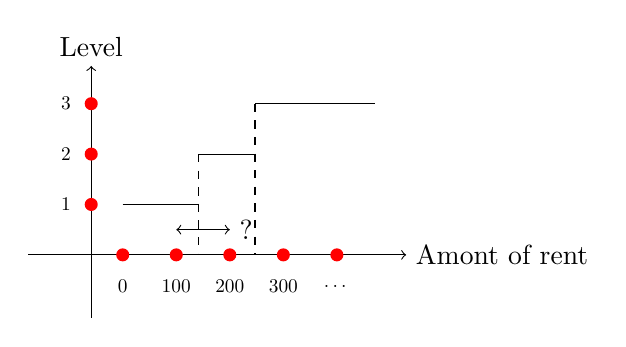
\begin{tikzpicture}[scale=0.8]
      \draw[->] (-1,0) -- (5,0) node[right] {Amont of rent};
      \draw[->] (0,-1) -- (0,3) node[above] {Level};

		\node[scale=0.5,red,circle, fill] (x1) at  (0.5,0) {};
		\node[scale=0.5,red,circle, fill] (x2) at  (1.35,0) {};
		\node[scale=0.5,red,circle, fill] (x3) at  (2.2,0) {};
		\node[scale=0.5,red,circle, fill] (x4) at  (3.05,0) {};
		\node[scale=0.5,red,circle, fill] (x5) at  (3.9,0) {};

		\node[scale=0.7] (x1) at  (0.5,-0.5) {$0$};
		\node[scale=0.7] (x2) at  (1.35,-0.5) {$100$};
		\node[scale=0.7] (x3) at  (2.2,-0.5) {$200$};
		\node[scale=0.7] (x4) at  (3.05,-0.5) {$300$};
		\node[scale=0.7] (x5) at  (3.9,-0.5) {\ldots};


		\node[scale=0.5,red,circle, fill] (x1) at  (0,0.8) {};
		\node[scale=0.5,red,circle, fill] (x2) at  (0,1.6) {};
		\node[scale=0.5,red,circle, fill] (x3) at  (0,2.4) {};

		\node[scale=0.7] (x1) at  (-0.4,0.8) {$1$};
		\node[scale=0.7] (x2) at  (-0.4,1.6) {$2$};
		\node[scale=0.7] (x3) at  (-0.4,2.4) {$3$};

      \draw[-] (0.5,0.8) -- (1.7,0.8);
      \draw[-] (1.7,1.6) -- (2.6,1.6);
      \draw[-] (2.6,2.4) -- (4.5,2.4);

      \draw[dashed] (1.7,1.6) -- (1.7,0);
      \draw[dashed] (2.6,2.4) -- (2.6,0);

      \draw[<-] (1.35,0.4) -- (1.7,0.4);
      \draw[->] (1.7,0.4) -- (2.2,0.4) node[right] {?};

\end{tikzpicture}
\caption{If the admissible quantizations are those displayed in red, and the estimated cutpoints are the dashed lines, which ``rounding'' shall be chosen?}
\label{fig:constraint1}
\end{subfigure}
\begin{subfigure}[t]{0.5\textwidth}
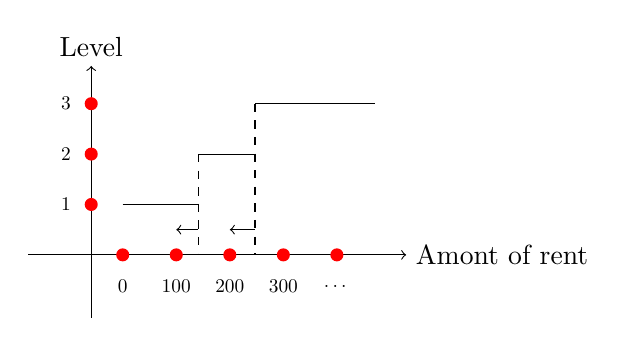
\begin{tikzpicture}[scale=0.8]
      \draw[->] (-1,0) -- (5,0) node[right] {Amont of rent};
      \draw[->] (0,-1) -- (0,3) node[above] {Level};

		\node[scale=0.5,red,circle, fill] (x1) at  (0.5,0) {};
		\node[scale=0.5,red,circle, fill] (x2) at  (1.35,0) {};
		\node[scale=0.5,red,circle, fill] (x3) at  (2.2,0) {};
		\node[scale=0.5,red,circle, fill] (x4) at  (3.05,0) {};
		\node[scale=0.5,red,circle, fill] (x5) at  (3.9,0) {};

		\node[scale=0.7] (x1) at  (0.5,-0.5) {$0$};
		\node[scale=0.7] (x2) at  (1.35,-0.5) {$100$};
		\node[scale=0.7] (x3) at  (2.2,-0.5) {$200$};
		\node[scale=0.7] (x4) at  (3.05,-0.5) {$300$};
		\node[scale=0.7] (x5) at  (3.9,-0.5) {\ldots};


		\node[scale=0.5,red,circle, fill] (x1) at  (0,0.8) {};
		\node[scale=0.5,red,circle, fill] (x2) at  (0,1.6) {};
		\node[scale=0.5,red,circle, fill] (x3) at  (0,2.4) {};

		\node[scale=0.7] (x1) at  (-0.4,0.8) {$1$};
		\node[scale=0.7] (x2) at  (-0.4,1.6) {$2$};
		\node[scale=0.7] (x3) at  (-0.4,2.4) {$3$};

      \draw[-] (0.5,0.8) -- (1.7,0.8);
      \draw[-] (1.7,1.6) -- (2.6,1.6);
      \draw[-] (2.6,2.4) -- (4.5,2.4);

      \draw[dashed] (1.7,1.6) -- (1.7,0);
      \draw[dashed] (2.6,2.4) -- (2.6,0);

      \draw[<-] (1.35,0.4) -- (1.7,0.4);
      \draw[<-] (2.2,0.4) -- (2.6,0.4);

\end{tikzpicture}
\caption{In this setting, rounding has no side effect.}
\label{fig:constraint2}
\end{subfigure}
\begin{subfigure}[t]{0.5\textwidth}
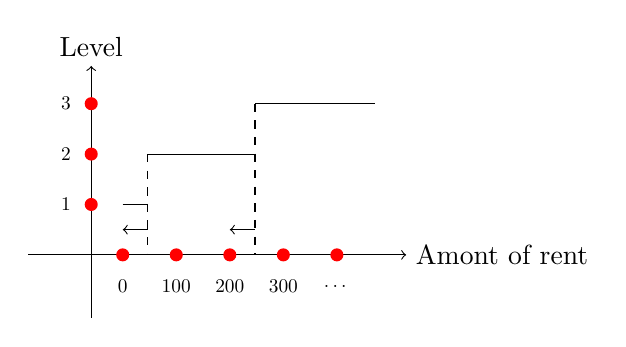
\begin{tikzpicture}[scale=0.8]
      \draw[->] (-1,0) -- (5,0) node[right] {Amont of rent};
      \draw[->] (0,-1) -- (0,3) node[above] {Level};

		\node[scale=0.5,red,circle, fill] (x1) at  (0.5,0) {};
		\node[scale=0.5,red,circle, fill] (x2) at  (1.35,0) {};
		\node[scale=0.5,red,circle, fill] (x3) at  (2.2,0) {};
		\node[scale=0.5,red,circle, fill] (x4) at  (3.05,0) {};
		\node[scale=0.5,red,circle, fill] (x5) at  (3.9,0) {};

		\node[scale=0.7] (x1) at  (0.5,-0.5) {$0$};
		\node[scale=0.7] (x2) at  (1.35,-0.5) {$100$};
		\node[scale=0.7] (x3) at  (2.2,-0.5) {$200$};
		\node[scale=0.7] (x4) at  (3.05,-0.5) {$300$};
		\node[scale=0.7] (x5) at  (3.9,-0.5) {\ldots};


		\node[scale=0.5,red,circle, fill] (x1) at  (0,0.8) {};
		\node[scale=0.5,red,circle, fill] (x2) at  (0,1.6) {};
		\node[scale=0.5,red,circle, fill] (x3) at  (0,2.4) {};

		\node[scale=0.7] (x1) at  (-0.4,0.8) {$1$};
		\node[scale=0.7] (x2) at  (-0.4,1.6) {$2$};
		\node[scale=0.7] (x3) at  (-0.4,2.4) {$3$};

      \draw[-] (0.5,0.8) -- (0.9,0.8);
      \draw[-] (0.9,1.6) -- (2.6,1.6);
      \draw[-] (2.6,2.4) -- (4.5,2.4);

      \draw[dashed] (0.9,1.6) -- (0.9,0);
      \draw[dashed] (2.6,2.4) -- (2.6,0);

      \draw[<-] (0.5,0.4) -- (0.9,0.4);
      \draw[<-] (2.2,0.4) -- (2.6,0.4);

\end{tikzpicture}
\caption{The first level is ``collapsed'' and disappears, with possible consequences to the predictive task.}
\label{fig:constraint3}
\end{subfigure}
\begin{subfigure}[t]{0.5\textwidth}
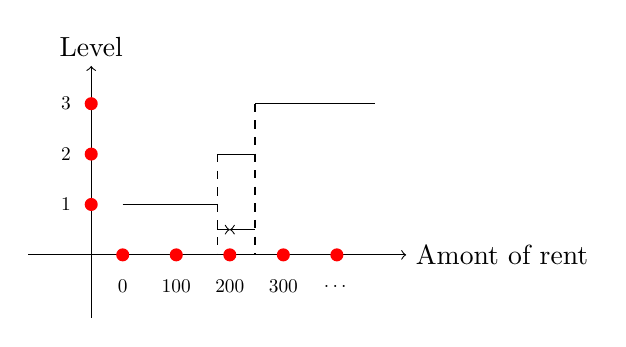
\begin{tikzpicture}[scale=0.8]
      \draw[->] (-1,0) -- (5,0) node[right] {Amont of rent};
      \draw[->] (0,-1) -- (0,3) node[above] {Level};

		\node[scale=0.5,red,circle, fill] (x1) at  (0.5,0) {};
		\node[scale=0.5,red,circle, fill] (x2) at  (1.35,0) {};
		\node[scale=0.5,red,circle, fill] (x3) at  (2.2,0) {};
		\node[scale=0.5,red,circle, fill] (x4) at  (3.05,0) {};
		\node[scale=0.5,red,circle, fill] (x5) at  (3.9,0) {};

		\node[scale=0.7] (x1) at  (0.5,-0.5) {$0$};
		\node[scale=0.7] (x2) at  (1.35,-0.5) {$100$};
		\node[scale=0.7] (x3) at  (2.2,-0.5) {$200$};
		\node[scale=0.7] (x4) at  (3.05,-0.5) {$300$};
		\node[scale=0.7] (x5) at  (3.9,-0.5) {\ldots};


		\node[scale=0.5,red,circle, fill] (x1) at  (0,0.8) {};
		\node[scale=0.5,red,circle, fill] (x2) at  (0,1.6) {};
		\node[scale=0.5,red,circle, fill] (x3) at  (0,2.4) {};

		\node[scale=0.7] (x1) at  (-0.4,0.8) {$1$};
		\node[scale=0.7] (x2) at  (-0.4,1.6) {$2$};
		\node[scale=0.7] (x3) at  (-0.4,2.4) {$3$};

      \draw[-] (0.5,0.8) -- (2,0.8);
      \draw[-] (2,1.6) -- (2.6,1.6);
      \draw[-] (2.6,2.4) -- (4.5,2.4);

      \draw[dashed] (2,1.6) -- (2,0);
      \draw[dashed] (2.6,2.4) -- (2.6,0);

      \draw[<-] (2.2,0.4) -- (2,0.4);
      \draw[<-] (2.2,0.4) -- (2.6,0.4);

\end{tikzpicture}
\caption{The narrow middle level is collapsed, also with possible predictive consequences, since \textit{e.g.}\ rent amounts are often very concentrated around their mean.}
\label{fig:constraint4}
\end{subfigure}
\caption{Different settings of estimated quantizations and the consequences of constraints on the set of admissible cutpoints.}
\label{fig:constraint}
\end{figure}

\subsection{Wrapping up}

Feature quantization (discretization for continuous features, grouping of factor levels for categorical ones) in a supervised multivariate classification is a recurring problem in many industrial contexts. This setting was formalized as a highly combinatorial representation learning problem and a new algorithmic approach, named \textit{glmdisc}, has been proposed as a sensible approximation of a classical statistical information criterion.

The first proposed implementation relies on the use of a neural network of particular architecture and specifically a softmax approximation of each discretized or grouped feature. The second proposed implementation relies on an SEM algorithm and a polytomic multiclass \gls{lr} approximation in the same flavor as the softmax. These proposals can alternatively be replaced by any other univariate multiclass predictive model, which make them flexible and adaptable to other problems. Prediction of the target feature, given quantized features, was exemplified with \gls{lr}, although here as well, it can be swapped with any other supervised classification model.

The experiments showed that, as was sensed empirically by statisticians in the field of \textit{Credit Scoring}, discretization and grouping can indeed provide better models than standard \gls{lr}. This novel approach allows practitioners to have a fully automated and statistically well-grounded tool that achieves better performance than \textit{ad hoc} industrial practices at the price of decent computing time but much less of the practitioner's valuable time.

As described in the introduction, \gls{lr} is additive in its inputs which does not allow to take into account conditional dependency, as stated by~\cite{berry2010testing}. This problem is often dealt with by sparsely introducing ``interactions'', \textit{i.e.}\ products of two features. This leads again to a model selection challenge on a highly combinatorial discrete space that could be solved with a similar approach. In a broader context with no restriction on the predictive model, \cite{tsang2018detecting} already made use of neural networks to estimate the presence or absence of statistical interactions. I take another approach in the subsequent chapter where I tackle the parsimonious addition of pairwise interactions among quantized features, that might influence the quantization process introduced in this work, is a future area of research.




\printbibliography[heading=subbibliography, title=References of Chapter 3]

